%********************************************%
%*       Generated from PreTeXt source      *%
%*       on 2025-09-15T17:18:55-04:00       *%
%*   A recent stable commit (2022-07-01):   *%
%* 6c761d3dba23af92cba35001c852aac04ae99a5f *%
%*                                          *%
%*         https://pretextbook.org          *%
%*                                          *%
%********************************************%
\documentclass[oneside,10pt,]{tufte-book}
%% Custom Preamble Entries, early (use latex.preamble.early)
%% Default LaTeX packages
%%   1.  always employed (or nearly so) for some purpose, or
%%   2.  a stylewriter may assume their presence
%\usepackage{geometry}
%% Some aspects of the preamble are conditional,
%% the LaTeX engine is one such determinant
\usepackage{ifthen}
%% etoolbox has a variety of modern conveniences
\usepackage{etoolbox}
\usepackage{ifxetex,ifluatex}
%% Raster graphics inclusion
\usepackage{graphicx}
%% Color support, xcolor package
%% Always loaded, for: add/delete text, author tools
%% Here, since tcolorbox loads tikz, and tikz loads xcolor
\PassOptionsToPackage{usenames,dvipsnames,svgnames,table}{xcolor}
%\usepackage{xcolor}
%% begin: defined colors, via xcolor package, for styling
%% end: defined colors, via xcolor package, for styling
%% Colored boxes, and much more, though mostly styling
%% skins library provides "enhanced" skin, employing tikzpicture
%% boxes may be configured as "breakable" or "unbreakable"
%% "raster" controls grids of boxes, aka side-by-side
\usepackage{tcolorbox}
\tcbuselibrary{skins}
\tcbuselibrary{breakable}
\tcbuselibrary{raster}
%% We load some "stock" tcolorbox styles that we use a lot
%% Placement here is provisional, there will be some color work also
%% First, black on white, no border, transparent, but no assumption about titles
\tcbset{ bwminimalstyle/.style={size=minimal, boxrule=-0.3pt, frame empty,
colback=white, colbacktitle=white, coltitle=black, opacityfill=0.0} }
%% Second, bold title, run-in to text/paragraph/heading
%% Space afterwards will be controlled by environment,
%% independent of constructions of the tcb title
%% Places \blocktitlefont onto many block titles
\tcbset{ runintitlestyle/.style={fonttitle=\blocktitlefont\upshape\bfseries, attach title to upper} }
%% Spacing prior to each exercise, anywhere
\tcbset{ exercisespacingstyle/.style={before skip={1.5ex plus 0.5ex}} }
%% Spacing prior to each block
\tcbset{ blockspacingstyle/.style={before skip={2.0ex plus 0.5ex}} }
%% xparse allows the construction of more robust commands,
%% this is a necessity for isolating styling and behavior
%% The tcolorbox library of the same name loads the base library
\tcbuselibrary{xparse}
%% The tcolorbox library loads TikZ, its calc package is generally useful,
%% and is necessary for some smaller documents that use partial tcolor boxes
%% See:  https://github.com/PreTeXtBook/pretext/issues/1624
\usetikzlibrary{calc}
%% We use some more exotic tcolorbox keys to restore indentation to parboxes
\tcbuselibrary{hooks}
%% Save default paragraph indentation and parskip for use later, when adjusting parboxes
\newlength{\normalparindent}
\newlength{\normalparskip}
\AtBeginDocument{\setlength{\normalparindent}{\parindent}}
\AtBeginDocument{\setlength{\normalparskip}{\parskip}}
\newcommand{\setparstyle}{\setlength{\parindent}{\normalparindent}\setlength{\parskip}{\normalparskip}}%% Hyperref should be here, but likes to be loaded late
%%
%% Inline math delimiters, \(, \), need to be robust
%% 2016-01-31:  latexrelease.sty  supersedes  fixltx2e.sty
%% If  latexrelease.sty  exists, bugfix is in kernel
%% If not, bugfix is in  fixltx2e.sty
%% See:  https://tug.org/TUGboat/tb36-3/tb114ltnews22.pdf
%% and read "Fewer fragile commands" in distribution's  latexchanges.pdf
\IfFileExists{latexrelease.sty}{}{\usepackage{fixltx2e}}
%% shorter subnumbers in some side-by-side require manipulations
\usepackage{xstring}
%% Footnote counters and part/chapter counters are manipulated
%% April 2018:  chngcntr  commands now integrated into the kernel,
%% but circa 2018/2019 the package would still try to redefine them,
%% so we need to do the work of loading conditionally for old kernels.
%% From version 1.1a,  chngcntr  should detect defintions made by LaTeX kernel.
\ifdefined\counterwithin
\else
    \usepackage{chngcntr}
\fi
%% Text height identically 9 inches, text width varies on point size
%% See Bringhurst 2.1.1 on measure for recommendations
%% 75 characters per line (count spaces, punctuation) is target
%% which is the upper limit of Bringhurst's recommendations
%\geometry{letterpaper,total={340pt,9.0in}}
%% Custom Page Layout Adjustments (use publisher page-geometry entry)
%% This LaTeX file may be compiled with pdflatex, xelatex, or lualatex executables
%% LuaTeX is not explicitly supported, but we do accept additions from knowledgeable users
%% The conditional below provides  pdflatex  specific configuration last
%% begin: engine-specific capabilities
\ifthenelse{\boolean{xetex} \or \boolean{luatex}}{%
%% begin: xelatex and lualatex-specific default configuration
\ifxetex\usepackage{xltxtra}\fi
%% realscripts is the only part of xltxtra relevant to lualatex 
\ifluatex\usepackage{realscripts}\fi
%% end:   xelatex and lualatex-specific default configuration
}{
%% begin: pdflatex-specific default configuration
%% We assume a PreTeXt XML source file may have Unicode characters
%% and so we ask LaTeX to parse a UTF-8 encoded file
%% This may work well for accented characters in Western language,
%% but not with Greek, Asian languages, etc.
%% When this is not good enough, switch to the  xelatex  engine
%% where Unicode is better supported (encouraged, even)
\usepackage[utf8]{inputenc}
%% end: pdflatex-specific default configuration
}
%% end:   engine-specific capabilities
%%
%% Fonts.  Conditional on LaTex engine employed.
%% Default Text Font: The Latin Modern fonts are
%% "enhanced versions of the [original TeX] Computer Modern fonts."
%% We use them as the default text font for PreTeXt output.
%% Default Monospace font: Inconsolata (aka zi4)
%% Sponsored by TUG: http://levien.com/type/myfonts/inconsolata.html
%% Loaded for documents with intentional objects requiring monospace
%% See package documentation for excellent instructions
%% fontspec will work universally if we use filename to locate OTF files
%% Loads the "upquote" package as needed, so we don't have to
%% Upright quotes might come from the  textcomp  package, which we also use
%% We employ the shapely \ell to match Google Font version
%% pdflatex: "varl" package option produces shapely \ell
%% pdflatex: "var0" package option produces plain zero (not used)
%% pdflatex: "varqu" package option produces best upright quotes
%% xelatex,lualatex: add OTF StylisticSet 1 for shapely \ell
%% xelatex,lualatex: add OTF StylisticSet 2 for plain zero (not used)
%% xelatex,lualatex: add OTF StylisticSet 3 for upright quotes
%%
%% Automatic Font Control
%% Portions of a document, are, or may, be affected by defined commands
%% These are perhaps more flexible when using  xelatex  rather than  pdflatex
%% The following definitions are meant to be re-defined in a style, using \renewcommand
%% They are scoped when employed (in a TeX group), and so should not be defined with an argument
\newcommand{\divisionfont}{\relax}
\newcommand{\blocktitlefont}{\relax}
\newcommand{\contentsfont}{\relax}
\newcommand{\pagefont}{\relax}
\newcommand{\tabularfont}{\relax}
\newcommand{\xreffont}{\relax}
\newcommand{\titlepagefont}{\relax}
%%
\ifthenelse{\boolean{xetex} \or \boolean{luatex}}{%
%% begin: font setup and configuration for use with xelatex
%% Generally, xelatex is necessary for non-Western fonts
%% fontspec package provides extensive control of system fonts,
%% meaning *.otf (OpenType), and apparently *.ttf (TrueType)
%% that live *outside* your TeX/MF tree, and are controlled by your *system*
%% (it is possible that a TeX distribution will place fonts in a system location)
%%
%% The fontspec package is the best vehicle for using different fonts in  xelatex
%% So we load it always, no matter what a publisher or style might want
%%
\usepackage{fontspec}
%%
%% begin: xelatex main font ("font-xelatex-main" template)
%% Latin Modern Roman is the default font for xelatex and so is loaded with a TU encoding
%% *in the format* so we can't touch it, only perhaps adjust it later
%% in one of two ways (then known by NFSS names such as "lmr")
%% (1) via NFSS with font family names such as "lmr" and "lmss"
%% (2) via fontspec with commands like \setmainfont{Latin Modern Roman}
%% The latter requires the font to be known at the system-level by its font name,
%% but will give access to OTF font features through optional arguments
%% https://tex.stackexchange.com/questions/470008/
%% where-and-how-does-fontspec-sty-specify-the-default-font-latin-modern-roman
%% http://tex.stackexchange.com/questions/115321
%% /how-to-optimize-latin-modern-font-with-xelatex
%%
%% end:   xelatex main font ("font-xelatex-main" template)
%% begin: xelatex mono font ("font-xelatex-mono" template)
%% (conditional on non-trivial uses being present in source)
\IfFontExistsTF{Inconsolatazi4-Regular.otf}{}{\GenericError{}{The font "Inconsolatazi4-Regular.otf" requested by PreTeXt output is not available.  Either a file cannot be located in default locations via a filename, or a font is not known by its name as part of your system.}{Consult the PreTeXt Guide for help with LaTeX fonts.}{}}
\IfFontExistsTF{Inconsolatazi4-Bold.otf}{}{\GenericError{}{The font "Inconsolatazi4-Bold.otf" requested by PreTeXt output is not available.  Either a file cannot be located in default locations via a filename, or a font is not known by its name as part of your system.}{Consult the PreTeXt Guide for help with LaTeX fonts.}{}}
\usepackage{zi4}
\setmonofont[BoldFont=Inconsolatazi4-Bold.otf,StylisticSet={1,3}]{Inconsolatazi4-Regular.otf}
%% end:   xelatex mono font ("font-xelatex-mono" template)
%% begin: xelatex font adjustments ("font-xelatex-style" template)
%% end:   xelatex font adjustments ("font-xelatex-style" template)
%%
%% Extensive support for other languages
\usepackage{polyglossia}
%% Set main/default language based on pretext/@xml:lang value
%% document language code is "en-US", US English
%% usmax variant has extra hypenation
\setmainlanguage[variant=usmax]{english}
%% Enable secondary languages based on discovery of @xml:lang values
%% Enable fonts/scripts based on discovery of @xml:lang values
%% Western languages should be ably covered by Latin Modern Roman
%% end:   font setup and configuration for use with xelatex
}{%
%% begin: font setup and configuration for use with pdflatex
%% begin: pdflatex main font ("font-pdflatex-main" template)
\usepackage{lmodern}
\usepackage[T1]{fontenc}
%% end:   pdflatex main font ("font-pdflatex-main" template)
%% begin: pdflatex mono font ("font-pdflatex-mono" template)
%% (conditional on non-trivial uses being present in source)
\usepackage[varqu,varl]{inconsolata}
%% end:   pdflatex mono font ("font-pdflatex-mono" template)
%% begin: pdflatex font adjustments ("font-pdflatex-style" template)
%% end:   pdflatex font adjustments ("font-pdflatex-style" template)
%% end:   font setup and configuration for use with pdflatex
}
%% Micromanage spacing, etc.  The named "microtype-options"
%% template may be employed to fine-tune package behavior
\usepackage{microtype}
%% Symbols, align environment, commutative diagrams, bracket-matrix
\usepackage{amsmath}
\usepackage{amscd}
\usepackage{amssymb}
%% allow page breaks within display mathematics anywhere
%% level 4 is maximally permissive
%% this is exactly the opposite of AMSmath package philosophy
%% there are per-display, and per-equation options to control this
%% split, aligned, gathered, and alignedat are not affected
\allowdisplaybreaks[4]
%% allow more columns to a matrix
%% can make this even bigger by overriding with  latex.preamble.late  processing option
\setcounter{MaxMatrixCols}{30}
%%
%%
%% Division Titles, and Page Headers/Footers
%% titlesec package, loading "titleps" package cooperatively
%% See code comments about the necessity and purpose of "explicit" option.
%% The "newparttoc" option causes a consistent entry for parts in the ToC 
%% file, but it is only effective if there is a \titleformat for \part.
%% "pagestyles" loads the  titleps  package cooperatively.
%\usepackage[explicit, newparttoc, pagestyles]{titlesec}
%% The companion titletoc package for the ToC.
\usepackage{titletoc}
%% Fixes a bug with transition from chapters to appendices in a "book"
%% See generating XSL code for more details about necessity
%\newtitlemark{\chaptertitlename}
%% begin: customizations of page styles via the modal "titleps-style" template
%% Designed to use commands from the LaTeX "titleps" package
%% Plain pages should have the same font for page numbers
%\renewpagestyle{plain}{%
%\setfoot{}{\pagefont\thepage}{}%
%}%
%% Single pages as in default LaTeX
%\renewpagestyle{headings}{%
%\sethead{\pagefont\slshape\MakeUppercase{\ifthechapter{\chaptertitlename\space\thechapter.\space}{}\chaptertitle}}{}{\pagefont\thepage}%
%}%
%\pagestyle{headings}
%% end: customizations of page styles via the modal "titleps-style" template
%%
%% Create globally-available macros to be provided for style writers
%% These are redefined for each occurence of each division
\newcommand{\divisionnameptx}{\relax}%
\newcommand{\titleptx}{\relax}%
\newcommand{\subtitleptx}{\relax}%
\newcommand{\shortitleptx}{\relax}%
\newcommand{\authorsptx}{\relax}%
\newcommand{\epigraphptx}{\relax}%
%% Create environments for possible occurences of each division
%% Environment for a PTX "preface" at the level of a LaTeX "chapter"
\NewDocumentEnvironment{preface}{mmmmmmm}
{%
\renewcommand{\divisionnameptx}{#1}%
\renewcommand{\titleptx}{#2}%
\renewcommand{\subtitleptx}{#3}%
\renewcommand{\shortitleptx}{#4}%
\renewcommand{\authorsptx}{#5}%
\renewcommand{\epigraphptx}{#6}%
\chapter*{#2}%
\addcontentsline{toc}{chapter}{#4}
\label{#7}%
}{}%
%% Environment for a PTX "acknowledgement" at the level of a LaTeX "chapter"
\NewDocumentEnvironment{acknowledgement}{mmmmmmm}
{%
\renewcommand{\divisionnameptx}{#1}%
\renewcommand{\titleptx}{#2}%
\renewcommand{\subtitleptx}{#3}%
\renewcommand{\shortitleptx}{#4}%
\renewcommand{\authorsptx}{#5}%
\renewcommand{\epigraphptx}{#6}%
\chapter*{#2}%
\addcontentsline{toc}{chapter}{#4}
\label{#7}%
}{}%
%% Environment for a PTX "part" at the level of a LaTeX "part"
\NewDocumentEnvironment{partptx}{mmmmmmm}
{%
\renewcommand{\divisionnameptx}{#1}%
\renewcommand{\titleptx}{#2}%
\renewcommand{\subtitleptx}{#3}%
\renewcommand{\shortitleptx}{#4}%
\renewcommand{\authorsptx}{#5}%
\renewcommand{\epigraphptx}{#6}%
\part[{#4}]{#2}%
\label{#7}%
}{}%
%% Environment for a PTX "chapter" at the level of a LaTeX "chapter"
\NewDocumentEnvironment{chapterptx}{mmmmmmm}
{%
\renewcommand{\divisionnameptx}{#1}%
\renewcommand{\titleptx}{#2}%
\renewcommand{\subtitleptx}{#3}%
\renewcommand{\shortitleptx}{#4}%
\renewcommand{\authorsptx}{#5}%
\renewcommand{\epigraphptx}{#6}%
\chapter[{#4}]{#2}%
\label{#7}%
}{}%
%% Environment for a PTX "section" at the level of a LaTeX "section"
\NewDocumentEnvironment{sectionptx}{mmmmmmm}
{%
\renewcommand{\divisionnameptx}{#1}%
\renewcommand{\titleptx}{#2}%
\renewcommand{\subtitleptx}{#3}%
\renewcommand{\shortitleptx}{#4}%
\renewcommand{\authorsptx}{#5}%
\renewcommand{\epigraphptx}{#6}%
\section[{#4}]{#2}%
\label{#7}%
}{}%
%% Environment for a PTX "subsection" at the level of a LaTeX "subsection"
\NewDocumentEnvironment{subsectionptx}{mmmmmmm}
{%
\renewcommand{\divisionnameptx}{#1}%
\renewcommand{\titleptx}{#2}%
\renewcommand{\subtitleptx}{#3}%
\renewcommand{\shortitleptx}{#4}%
\renewcommand{\authorsptx}{#5}%
\renewcommand{\epigraphptx}{#6}%
\subsection[{#4}]{#2}%
\label{#7}%
}{}%
%% Environment for a PTX "appendix" at the level of a LaTeX "chapter"
\NewDocumentEnvironment{appendixptx}{mmmmmmm}
{%
\renewcommand{\divisionnameptx}{#1}%
\renewcommand{\titleptx}{#2}%
\renewcommand{\subtitleptx}{#3}%
\renewcommand{\shortitleptx}{#4}%
\renewcommand{\authorsptx}{#5}%
\renewcommand{\epigraphptx}{#6}%
\chapter[{#4}]{#2}%
\label{#7}%
}{}%
%%
%% Styles for six traditional LaTeX divisions
%\titleformat{\part}[display]
%{\divisionfont\Huge\bfseries\centering}{\divisionnameptx\space\thepart}{30pt}{\Huge#1}
%[{\Large\centering\authorsptx}]
%\titleformat{\chapter}[display]
%{\divisionfont\huge\bfseries}{\divisionnameptx\space\thechapter}{20pt}{\Huge#1}
%[{\Large\authorsptx}]
%\titleformat{name=\chapter,numberless}[display]
%{\divisionfont\huge\bfseries}{}{0pt}{#1}
%[{\Large\authorsptx}]
%\titlespacing*{\chapter}{0pt}{50pt}{40pt}
%\titleformat{\section}[hang]
%{\divisionfont\Large\bfseries}{\thesection}{1ex}{#1}
%[{\large\authorsptx}]
%\titleformat{name=\section,numberless}[block]
%{\divisionfont\Large\bfseries}{}{0pt}{#1}
%[{\large\authorsptx}]
%\titlespacing*{\section}{0pt}{3.5ex plus 1ex minus .2ex}{2.3ex plus .2ex}
%\titleformat{\subsection}[hang]
%{\divisionfont\large\bfseries}{\thesubsection}{1ex}{#1}
%[{\normalsize\authorsptx}]
%\titleformat{name=\subsection,numberless}[block]
%{\divisionfont\large\bfseries}{}{0pt}{#1}
%[{\normalsize\authorsptx}]
%\titlespacing*{\subsection}{0pt}{3.25ex plus 1ex minus .2ex}{1.5ex plus .2ex}
%\titleformat{\subsubsection}[hang]
%{\divisionfont\normalsize\bfseries}{\thesubsubsection}{1em}{#1}
%[{\small\authorsptx}]
%\titleformat{name=\subsubsection,numberless}[block]
%{\divisionfont\normalsize\bfseries}{}{0pt}{#1}
%[{\normalsize\authorsptx}]
%\titlespacing*{\subsubsection}{0pt}{3.25ex plus 1ex minus .2ex}{1.5ex plus .2ex}
%\titleformat{\paragraph}[hang]
%{\divisionfont\normalsize\bfseries}{\theparagraph}{1em}{#1}
%[{\small\authorsptx}]
%\titleformat{name=\paragraph,numberless}[block]
%{\divisionfont\normalsize\bfseries}{}{0pt}{#1}
%[{\normalsize\authorsptx}]
%\titlespacing*{\paragraph}{0pt}{3.25ex plus 1ex minus .2ex}{1.5em}
%%
%% Styles for five traditional LaTeX divisions
\titlecontents{part}%
[0pt]{\contentsmargin{0em}\addvspace{1pc}\contentsfont\bfseries}%
{\Large\thecontentslabel\enspace}{\Large}%
{}%
[\addvspace{.5pc}]%
\titlecontents{chapter}%
[0pt]{\contentsmargin{0em}\addvspace{1pc}\contentsfont\bfseries}%
{\large\thecontentslabel\enspace}{\large}%
{\hfill\bfseries\thecontentspage}%
[\addvspace{.5pc}]%
\dottedcontents{section}[3.8em]{\contentsfont}{2.3em}{1pc}%
\dottedcontents{subsection}[6.1em]{\contentsfont}{3.2em}{1pc}%
\dottedcontents{subsubsection}[9.3em]{\contentsfont}{4.3em}{1pc}%
%%
%% Begin: Semantic Macros
%% To preserve meaning in a LaTeX file
%%
%% \mono macro for content of "c", "cd", "tag", etc elements
%% Also used automatically in other constructions
%% Simply an alias for \texttt
%% Always defined, even if there is no need, or if a specific tt font is not loaded
\newcommand{\mono}[1]{\texttt{#1}}
%%
%% Following semantic macros are only defined here if their
%% use is required only in this specific document
%%
%% Used for warnings, typically bold and italic
\newcommand{\alert}[1]{\textbf{\textit{#1}}}
%% Used for inline definitions of terms
\newcommand{\terminology}[1]{\textbf{#1}}
%% End: Semantic Macros
%% Equation Numbering
%% Controlled by  numbering.equations.level  processing parameter
%% No adjustment here implies document-wide numbering
\numberwithin{equation}{chapter}
%% "tcolorbox" environment for a single image, occupying entire \linewidth
%% arguments are left-margin, width, right-margin, as multiples of
%% \linewidth, and are guaranteed to be positive and sum to 1.0
\tcbset{ imagestyle/.style={bwminimalstyle} }
\NewTColorBox{tcbimage}{mmm}{imagestyle,left skip=#1\linewidth,width=#2\linewidth}
%% Wrapper environment for tcbimage environment with a fourth argument
%% Fourth argument, if nonempty, is a vertical space adjustment
%% and implies image will be preceded by \leavevmode\nopagebreak
%% Intended use is for alignment with a list marker
\NewDocumentEnvironment{image}{mmmm}{\notblank{#4}{\leavevmode\nopagebreak\vspace{#4}}{}\begin{tcbimage}{#1}{#2}{#3}}{\end{tcbimage}%
}%% For improved tables
\usepackage{array}
%% Some extra height on each row is desirable, especially with horizontal rules
%% Increment determined experimentally
\setlength{\extrarowheight}{0.2ex}
%% Define variable thickness horizontal rules, full and partial
%% Thicknesses are 0.03, 0.05, 0.08 in the  booktabs  package
\newcommand{\hrulethin}  {\noalign{\hrule height 0.04em}}
\newcommand{\hrulemedium}{\noalign{\hrule height 0.07em}}
\newcommand{\hrulethick} {\noalign{\hrule height 0.11em}}
%% We preserve a copy of the \setlength package before other
%% packages (extpfeil) get a chance to load packages that redefine it
\let\oldsetlength\setlength
\newlength{\Oldarrayrulewidth}
\newcommand{\crulethin}[1]%
{\noalign{\global\oldsetlength{\Oldarrayrulewidth}{\arrayrulewidth}}%
\noalign{\global\oldsetlength{\arrayrulewidth}{0.04em}}\cline{#1}%
\noalign{\global\oldsetlength{\arrayrulewidth}{\Oldarrayrulewidth}}}%
\newcommand{\crulemedium}[1]%
{\noalign{\global\oldsetlength{\Oldarrayrulewidth}{\arrayrulewidth}}%
\noalign{\global\oldsetlength{\arrayrulewidth}{0.07em}}\cline{#1}%
\noalign{\global\oldsetlength{\arrayrulewidth}{\Oldarrayrulewidth}}}
\newcommand{\crulethick}[1]%
{\noalign{\global\oldsetlength{\Oldarrayrulewidth}{\arrayrulewidth}}%
\noalign{\global\oldsetlength{\arrayrulewidth}{0.11em}}\cline{#1}%
\noalign{\global\oldsetlength{\arrayrulewidth}{\Oldarrayrulewidth}}}
%% Single letter column specifiers defined via array package
\newcolumntype{A}{!{\vrule width 0.04em}}
\newcolumntype{B}{!{\vrule width 0.07em}}
\newcolumntype{C}{!{\vrule width 0.11em}}
%% tcolorbox to place tabular outside of a sidebyside
\tcbset{ tabularboxstyle/.style={bwminimalstyle,} }
\newtcolorbox{tabularbox}[3]{tabularboxstyle, left skip=#1\linewidth, width=#2\linewidth,}
%% Footnote Numbering
%% Specified by numbering.footnotes.level
%% Undo counter reset by chapter for a book
\counterwithout{footnote}{chapter}
\counterwithin*{footnote}{chapter}
%% More flexible list management, esp. for references
%% But also for specifying labels (i.e. custom order) on nested lists
\usepackage{enumitem}
%% Description lists as tcolorbox sidebyside
%% "dli" short for "description list item"
\newlength{\dlititlewidth}
\newlength{\dlimaxnarrowtitle}\setlength{\dlimaxnarrowtitle}{11ex}
\newlength{\dlimaxmediumtitle}\setlength{\dlimaxmediumtitle}{18ex}
\tcbset{ dlistyle/.style={sidebyside, sidebyside align=top seam, lower separated=false, bwminimalstyle, bottomtitle=0.75ex, after skip=1.5ex, boxsep=0pt, left=0pt, right=0pt, top=0pt, bottom=0pt} }
\tcbset{ dlinarrowstyle/.style={dlistyle, lefthand width=\dlimaxnarrowtitle, sidebyside gap=1ex, halign=flush left, righttitle=10ex} }
\tcbset{ dlimediumstyle/.style={dlistyle, lefthand width=\dlimaxmediumtitle, sidebyside gap=4ex, halign=flush right} }
\NewDocumentEnvironment{descriptionlist}{}{\par\vspace*{1.5ex}}{\par\vspace*{1.5ex}}%
%% begin enviroment has an if/then to open the tcolorbox
\NewDocumentEnvironment{dlinarrow}{mm}{%
\settowidth{\dlititlewidth}{{\textbf{#1}}}%
\ifthenelse{\dlititlewidth > \dlimaxnarrowtitle}%
{\begin{tcolorbox}[title={\textbf{#1}}, phantom={\hypertarget{#2}{}}, dlinarrowstyle]\tcblower}%
{\begin{tcolorbox}[dlinarrowstyle, phantom={\hypertarget{#2}{}}]\textbf{#1}\tcblower}%
}%
{\end{tcolorbox}}%
%% medium option is simpler
\NewDocumentEnvironment{dlimedium}{mm}%
{\begin{tcolorbox}[dlimediumstyle, phantom={\hypertarget{#2}{}}]\textbf{#1}\tcblower}%
{\end{tcolorbox}}%
%% hyperref driver does not need to be specified, it will be detected
%% Footnote marks in tcolorbox have broken linking under
%% hyperref, so it is necessary to turn off all linking
%% It *must* be given as a package option, not with \hypersetup
\usepackage[hyperfootnotes=false]{hyperref}
%% configure hyperref's  \href{}{}  and  \nolinkurl  to match listings' inline verbatim
\renewcommand\UrlFont{\small\ttfamily}
%% Hyperlinking active in electronic PDFs, all links without surrounding boxes and blue
\hypersetup{colorlinks=true,linkcolor=blue,citecolor=blue,filecolor=blue,urlcolor=blue}
%% Less-clever names for hyperlinks are more reliable, *especially* for structural parts
%% See comments in the code to learn more about the importance of this setting
\hypersetup{hypertexnames=false}
%%The  hypertexnames  setting then confuses the hyperlinking from the index
%%This patch resolves the incorrect links, see code for StackExchange post.
\makeatletter
\patchcmd\Hy@EveryPageBoxHook{\Hy@EveryPageAnchor}{\Hy@hypertexnamestrue\Hy@EveryPageAnchor}{}{\fail}
\makeatother
\hypersetup{pdftitle={Functions at Work}}
%% If you manually remove hyperref, leave in this next command
%% This will allow LaTeX compilation, employing this no-op command
\providecommand\phantomsection{}
%% Division Numbering: Chapters, Sections, Subsections, etc
%% Division numbers may be turned off at some level ("depth")
%% A section *always* has depth 1, contrary to us counting from the document root
%% The latex default is 3.  If a larger number is present here, then
%% removing this command may make some cross-references ambiguous
%% The precursor variable $numbering-maxlevel is checked for consistency in the common XSL file
\setcounter{secnumdepth}{3}
%%
%% AMS "proof" environment is no longer used, but we leave previously
%% implemented \qedhere in place, should the LaTeX be recycled
\newcommand{\qedhere}{\relax}
%%
%% A faux tcolorbox whose only purpose is to provide common numbering
%% facilities for most blocks (possibly not projects, 2D displays)
%% Controlled by  numbering.theorems.level  processing parameter
\newtcolorbox[auto counter, number within=chapter]{block}{}
%%
%% This document is set to number PROJECT-LIKE on a separate numbering scheme
%% So, a faux tcolorbox whose only purpose is to provide this numbering
%% Controlled by  numbering.projects.level  processing parameter
\newtcolorbox[auto counter, number within=chapter]{project-distinct}{}
%% A faux tcolorbox whose only purpose is to provide common numbering
%% facilities for 2D displays which are subnumbered as part of a "sidebyside"
\makeatletter
\newtcolorbox[auto counter, number within=tcb@cnt@block, number freestyle={\noexpand\thetcb@cnt@block(\noexpand\alph{\tcbcounter})}]{subdisplay}{}
\makeatother
%%
%% tcolorbox, with styles, for THEOREM-LIKE
%%
%% proposition: fairly simple numbered block/structure
\tcbset{ propositionstyle/.style={bwminimalstyle, runintitlestyle, blockspacingstyle, after title={\space}, before upper app={\setparstyle}, } }
\newtcolorbox[use counter from=block]{proposition}[4]{title={{#1~\thetcbcounter\notblank{#2#3}{\space}{}\notblank{#2}{\space#2}{}\notblank{#3}{\space(#3)}{}}}, phantomlabel={#4}, breakable, after={\par}, fontupper=\itshape, propositionstyle, }
%% corollary: fairly simple numbered block/structure
\tcbset{ corollarystyle/.style={bwminimalstyle, runintitlestyle, blockspacingstyle, after title={\space}, before upper app={\setparstyle}, } }
\newtcolorbox[use counter from=block]{corollary}[4]{title={{#1~\thetcbcounter\notblank{#2#3}{\space}{}\notblank{#2}{\space#2}{}\notblank{#3}{\space(#3)}{}}}, phantomlabel={#4}, breakable, after={\par}, fontupper=\itshape, corollarystyle, }
%% theorem: fairly simple numbered block/structure
\tcbset{ theoremstyle/.style={bwminimalstyle, runintitlestyle, blockspacingstyle, after title={\space}, before upper app={\setparstyle}, } }
\newtcolorbox[use counter from=block]{theorem}[4]{title={{#1~\thetcbcounter\notblank{#2#3}{\space}{}\notblank{#2}{\space#2}{}\notblank{#3}{\space(#3)}{}}}, phantomlabel={#4}, breakable, after={\par}, fontupper=\itshape, theoremstyle, }
%%
%% tcolorbox, with styles, for PROOF-LIKE
%%
%% proof: title is a replacement
\tcbset{ proofstyle/.style={bwminimalstyle, fonttitle=\blocktitlefont\itshape, attach title to upper, after title={\space}, after upper={\space\space\hspace*{\stretch{1}}\(\blacksquare\)},
} }
\newtcolorbox{proof}[3]{title={\notblank{#2}{#2}{#1.}}, phantom={\hypertarget{#3}{}}, breakable, before upper app={\setparstyle}, after={\par}, proofstyle }
%%
%% tcolorbox, with styles, for AXIOM-LIKE
%%
%% axiom: fairly simple numbered block/structure
\tcbset{ axiomstyle/.style={bwminimalstyle, runintitlestyle, blockspacingstyle, after title={\space}, before upper app={\setparstyle}, } }
\newtcolorbox[use counter from=block]{axiom}[4]{title={{#1~\thetcbcounter\notblank{#2#3}{\space}{}\notblank{#2}{\space#2}{}\notblank{#3}{\space(#3)}{}}}, phantomlabel={#4}, breakable, after={\par}, fontupper=\itshape, axiomstyle, }
%%
%% tcolorbox, with styles, for DEFINITION-LIKE
%%
%% definition: fairly simple numbered block/structure
\tcbset{ definitionstyle/.style={bwminimalstyle, runintitlestyle, blockspacingstyle, after title={\space}, before upper app={\setparstyle}, after upper={\space\space\hspace*{\stretch{1}}\(\lozenge\)}, } }
\newtcolorbox[use counter from=block]{definition}[3]{title={{#1~\thetcbcounter\notblank{#2}{\space\space#2}{}}}, phantomlabel={#3}, breakable, after={\par}, definitionstyle, }
%%
%% tcolorbox, with styles, for REMARK-LIKE
%%
%% insight: fairly simple numbered block/structure
\tcbset{ insightstyle/.style={bwminimalstyle, runintitlestyle, blockspacingstyle, after title={\space}, before upper app={\setparstyle}, } }
\newtcolorbox[use counter from=block]{insight}[3]{title={{#1~\thetcbcounter\notblank{#2}{\space\space#2}{}}}, phantomlabel={#3}, breakable, after={\par}, insightstyle, }
%% note: fairly simple numbered block/structure
\tcbset{ notestyle/.style={bwminimalstyle, runintitlestyle, blockspacingstyle, after title={\space}, before upper app={\setparstyle}, } }
\newtcolorbox[use counter from=block]{note}[3]{title={{#1~\thetcbcounter\notblank{#2}{\space\space#2}{}}}, phantomlabel={#3}, breakable, after={\par}, notestyle, }
%%
%% tcolorbox, with styles, for EXAMPLE-LIKE
%%
%% example: fairly simple numbered block/structure
\tcbset{ examplestyle/.style={bwminimalstyle, runintitlestyle, blockspacingstyle, after title={\space}, before upper app={\setparstyle}, after upper={\space\space\hspace*{\stretch{1}}\(\square\)}, } }
\newtcolorbox[use counter from=block]{example}[3]{title={{#1~\thetcbcounter\notblank{#2}{\space\space#2}{}}}, phantomlabel={#3}, breakable, after={\par}, examplestyle, }
%%
%% tcolorbox, with styles, for inline exercises
%%
%% inlineexercise: fairly simple numbered block/structure
\tcbset{ inlineexercisestyle/.style={bwminimalstyle, runintitlestyle, blockspacingstyle, after title={\space}, before upper app={\setparstyle}, } }
\newtcolorbox[use counter from=block]{inlineexercise}[3]{title={{#1~\thetcbcounter\notblank{#2}{\space\space#2}{}}}, phantomlabel={#3}, breakable, after={\par}, inlineexercisestyle, }
%%
%% tcolorbox, with styles, for PROJECT-LIKE
%%
%% exploration: fairly simple numbered block/structure
\tcbset{ explorationstyle/.style={bwminimalstyle, runintitlestyle, blockspacingstyle, after title={\space}, before upper app={\setparstyle}, } }
\newtcolorbox[use counter from=project-distinct]{exploration}[3]{title={{#1~\thetcbcounter\notblank{#2}{\space\space#2}{}}}, phantomlabel={#3}, breakable, after={\par}, explorationstyle, }
%%
%% tcolorbox, with styles, for GOAL-LIKE
%%
%% objectives: early in a subdivision, introduction/list/conclusion
\tcbset{ objectivesstyle/.style={bwminimalstyle, blockspacingstyle, fonttitle=\blocktitlefont\large\bfseries, toprule=0.1ex, toptitle=0.5ex, top=2ex, bottom=0.5ex, bottomrule=0.1ex} }
\newtcolorbox{objectives}[2]{title={#1}, phantomlabel={#2}, breakable, before upper app={\setparstyle}, objectivesstyle}
%%
%% tcolorbox, with styles, for ASIDE-LIKE
%%
%% aside: fairly simple un-numbered block/structure
\tcbset{ asidestyle/.style={bwminimalstyle, runintitlestyle, blockspacingstyle, after title={\space}, before upper app={\setparstyle}, } }
\newtcolorbox{aside}[3]{title={\notblank{#2}{#2}{}}, phantomlabel={#3}, breakable, before upper app={\setparstyle}, asidestyle}
%%
%% tcolorbox, with styles, for FIGURE-LIKE
%%
%% figureptx: 2-D display structure
\tcbset{ figureptxstyle/.style={bwminimalstyle, middle=1ex, blockspacingstyle, fontlower=\blocktitlefont} }
\newtcolorbox[use counter from=block]{figureptx}[4]{lower separated=false, before lower={{\textbf{#1~\thetcbcounter}\space#2}}, phantomlabel={#3}, unbreakable, figureptxstyle, }
%% tableptx: 2-D display structure
\tcbset{ tableptxstyle/.style={bwminimalstyle, middle=1ex, blockspacingstyle, coltitle=black, bottomtitle=2ex, titlerule=-0.3pt, fonttitle=\blocktitlefont, breakable} }
\newtcolorbox[use counter from=block]{tableptx}[4]{title={{\textbf{#1~\thetcbcounter}\space#2}}, phantomlabel={#3}, unbreakable, tableptxstyle, }
%%
%% xparse environments for introductions and conclusions of divisions
%%
%% introduction: in a structured division
\NewDocumentEnvironment{introduction}{m}
{\notblank{#1}{\noindent\textbf{#1}\space}{}}{\par\medskip}
%%
%% tcolorbox, with styles, for miscellaneous environments
%%
%% paragraphs: the terminal, pseudo-division
%% We use the lowest LaTeX traditional division
%\titleformat{\subparagraph}[runin]{\normalfont\normalsize\bfseries}{\thesubparagraph}{1em}{#1}
\titlespacing*{\subparagraph}{0pt}{3.25ex plus 1ex minus .2ex}{1em}
\NewDocumentEnvironment{paragraphs}{mm}
{\paragraph*{#1}\hypertarget{#2}{}}{}
%% assemblage: fairly simple un-numbered block/structure
\tcbset{ assemblagestyle/.style={size=normal, colback=white, colbacktitle=white, coltitle=black, colframe=black, rounded corners, titlerule=0.0pt, center title, fonttitle=\blocktitlefont\bfseries, blockspacingstyle, } }
\newtcolorbox{assemblage}[3]{title={\notblank{#2}{#2}{}}, phantomlabel={#3}, breakable, before upper app={\setparstyle}, assemblagestyle}
%% back colophon, at the very end, typically on its own page
\tcbset{ backcolophonstyle/.style={bwminimalstyle, blockspacingstyle, before skip=5ex, left skip=0.15\textwidth, right skip=0.15\textwidth, fonttitle=\blocktitlefont\large\bfseries, center title, halign=center, bottomtitle=2ex} }
\newtcolorbox{backcolophon}[2]{title={#1}, phantom={\hypertarget{#2}{}}, breakable, before upper app={\setparstyle}, backcolophonstyle}
%% Graphics Preamble Entries
\usepackage{tikz, pgfplots}
\usetikzlibrary{positioning,matrix,arrows}
\usetikzlibrary{shapes,decorations,shadows,fadings,patterns}
\usetikzlibrary{decorations.markings} 

\usetikzlibrary{arrows,calc,decorations.markings}

\pgfarrowsdeclarecombine*{|<}{>|}{latex}{latex}{|}{|}
\tikzset{dimen/.style={|<->|,>=latex,thin,every rectangle node/.style={fill=white,midway,font=\sffamily}},}

%%%% Begin: Set up TikZ Package and Styles %%%%
\tikzset{grid/.style={dotted}}
\tikzset{major gridlines/.style={thin}}
\tikzset{minor gridlines/.style={dotted, thick}}
\tikzset{vertical gridlines/.style={ultra thin}}
\tikzset{axes/.style={latex-latex}}
\tikzset{curve/.style={thick}}
\tikzset{open circle/.style={color=black, very thick, fill=white}}
\tikzset{closed circle/.style={color=black, very thick, fill=black}}
%%%% End: Set up TikZ Package and Styles %%%%

\def\drawtikzspline(#1,#2,#3,#4,#5,#6){ \draw[curve,domain=(#1):(#4)] plot (\x , { ( (((#3) + (#6))*(#1) - ((#3) + (#6))*(#4) - 2*(#2) + 2*(#5))/((#1)^3 - 3*((#1)^2)*(#4) + 3*(#1)*((#4)^2) - (#4)^3) )*((\x)^3) + ( -(((#3) + 2*(#6))*((#1)^2) + ((#3) - (#6))*(#1)*(#4) - (2*(#3) + (#6))*((#4)^2) - 3*((#1) + (#4))*(#2) + 3*((#1) + (#4))*(#5))/((#1)^3 - 3*((#1)^2)*(#4) + 3*(#1)*((#4)^2) - (#4)^3) ) *((\x)^2) + ( ((#6)*((#1)^3) + (2*(#3) + (#6))*((#1)^2)*(#4) - ((#3) + 2*(#6))*(#1)*((#4)^2) - (#3)*((#4)^3) - 6*(#1)*(#4)*(#2) + 6*(#1)*(#4)*(#5))/((#1)^3 - 3*((#1)^2)*(#4) + 3*(#1)*((#4)^2) - (#4)^3) ) * (\x) + ( -((#6)*((#1)^3)*(#4) + ((#3) - (#6))*((#1)^2)*(#4)^2 - (#3)*(#1)*((#4)^3) - (3*(#1)*((#4)^2) - (#4)^3)*(#2) - ((#1)^3 - 3*((#1)^2)*(#4))*(#5))/((#1)^3 - 3*((#1)^2)*(#4) + 3*(#1)*((#4)^2) - (#4)^3))}) }
%% If tikz has been loaded, replace ampersand with \amp macro
\ifdefined\tikzset
    \tikzset{ampersand replacement = \amp}
\fi
%% tcolorbox styles for sidebyside layout
\tcbset{ sbsstyle/.style={raster before skip=2.0ex, raster equal height=rows, raster force size=false, raster after skip=0.7\baselineskip} }
\tcbset{ sbspanelstyle/.style={bwminimalstyle, fonttitle=\blocktitlefont, before upper app={\setparstyle}} }
%% Enviroments for side-by-side and components
%% Necessary to use \NewTColorBox for boxes of the panels
%% "newfloat" environment to squash page-breaks within a single sidebyside
%% "xparse" environment for entire sidebyside
\NewDocumentEnvironment{sidebyside}{mmmm}
  {\begin{tcbraster}
    [sbsstyle,raster columns=#1,
    raster left skip=#2\linewidth,raster right skip=#3\linewidth,raster column skip=#4\linewidth]}
  {\end{tcbraster}}
%% "tcolorbox" environment for a panel of sidebyside
\NewTColorBox{sbspanel}{mO{top}}{sbspanelstyle,width=#1\linewidth,valign=#2}
%% Custom Preamble Entries, late (use latex.preamble.late)
%% extpfeil package for certain extensible arrows,
%% as also provided by MathJax extension of the same name
%% NB: this package loads mtools, which loads calc, which redefines
%%     \setlength, so it can be removed if it seems to be in the 
%%     way and your math does not use:
%%     
%%     \xtwoheadrightarrow, \xtwoheadleftarrow, \xmapsto, \xlongequal, \xtofrom
%%     
%%     we have had to be extra careful with variable thickness
%%     lines in tables, and so also load this package late
\usepackage{extpfeil}
%% Begin: Author-provided macros
%% (From  docinfo/macros  element)
%% Plus three from PTX for XML characters
\newcommand{\N}{\mathbb N}
\newcommand{\Z}{\mathbb Z}
\newcommand{\Q}{\mathbb Q}
\newcommand{\R}{\mathbb R}

\newcommand{\red}[1]{   {\color{red}   #1}   }
\newcommand{\blue}[1]{  {\color{blue}  #1}  }
\newcommand{\green}[1]{ {\color{green} #1} }

\newcommand{\ddx}[1]{ \dfrac{d}{dx} \Big[ #1 \Big]  } 
\newcommand{\ddt}[1]{ \dfrac{d}{dt} \Big[ #1 \Big]  } 
\newcommand{\ddu}[1]{ \dfrac{d}{du} \Big[ #1 \Big]  } 
\newcommand{\ddxfrac}[1]{ \dfrac{d}{dx} \left[ #1 \right]  } 
\newcommand{\D}[1]{ \Big[ #1 \Big]'  } 

\newcommand{\intdx}[1]{{\,\int#1\,\,dx}}
\newcommand{\dint}[1]{\displaystyle\intdx{#1}}

\def \tikzhistogram (#1,#2){\draw[fill=blue,opacity=0.3] ({#1+((\xtwo-\xmin)/5)},#2) rectangle ({#1-((\xtwo-\xmin)/5)},0); \draw[draw,thick] ({#1+((\xtwo-\xmin)/5)},#2) rectangle ({#1-((\xtwo-\xmin)/5)},0); \node[draw,fill=blue, circle,inner sep=2.5pt] at (#1,#2) {};}
\newcommand{\lt}{<}
\newcommand{\gt}{>}
\newcommand{\amp}{&}
%% End: Author-provided macros
\begin{document}
%% bottom alignment is explicit, since it normally depends on oneside, twoside
\raggedbottom
\frontmatter
%% begin: half-title
\thispagestyle{empty}
{\titlepagefont\centering
\vspace*{0.28\textheight}
{\Huge Functions at Work}\\[2\baselineskip]
{\LARGE Business Calculus}\\
}
\clearpage
%% end:   half-title
%% begin: title page
%% Inspired by Peter Wilson's "titleDB" in "titlepages" CTAN package
\thispagestyle{empty}
{\titlepagefont\centering
\vspace*{0.14\textheight}
%% Target for xref to top-level element is ToC
\addtocontents{toc}{\protect\hypertarget{home}{}}
{\Huge Functions at Work}\\[\baselineskip]
{\LARGE Business Calculus}\\[3\baselineskip]
{\Large Stephen Flood}\\[0.5\baselineskip]
{\Large Bridgewater State University}\\[3\baselineskip]
{\Large September 15, 2025}\\}
\clearpage
%% end:   title page
%% begin: copyright-page
\thispagestyle{empty}
\hypertarget{frontmatter-2}{}\vspace*{\stretch{2}}
\noindent\textcopyright{}2025\quad{}Stephen Flood\\[0.5\baselineskip]
\begin{image}{0.425}{0.15}{0.425}{}%

\includegraphics[width=\linewidth]{external/by-nc-sa.png}
\end{image}%
 This work is licensed under the Creative Commons Attribution-NonCommercial-ShareAlike 4.0 International. To view a copy of this license, visit \href{https://creativecommons.org/licenses/by-nc-sa/4.0/}{CreativeCommons.org}\footnote{\nolinkurl{creativecommons.org/licenses/by-nc-sa/4.0}\label{frontmatter-2-2-4-3}}\par\medskip
\vspace*{\stretch{1}}
\null\clearpage
%% end:   copyright-page
%% begin: dedication-page
\cleardoublepage
\thispagestyle{empty}
\vspace*{\stretch{1}}
\begin{center}\Large%
Dedicated to the champions of Open Educational Resources at Bridgewater State University and beyond, and to the developers of PreTeXt who developed and maintain the software that made this book possible.%
\end{center}
\vspace*{\stretch{2}}
\clearpage
%% end:   dedication-page
%
%
\typeout{************************************************}
\typeout{Preface  How to use this book}
\typeout{************************************************}
%
\begin{preface}{Preface}{How to use this book}{}{How to use this book}{}{}{to_the_student}
Welcome to Business Calculus. You are beginning an exciting adventure into a new kind of mathematics, one with more applications than you have seen in your previous courses, and one which will require new kinds of practice and problem solving.%
\par
This book is the result of many years of teaching and refining this course, with a particular focus on highlighting a variety of ways that this course can be of service to you in your future studies.%
\par
The large number of examples with full solutions are intended to aid you in your study of the topic.%
\begin{paragraphs}{The Promise of Active Reading.}{to_the_student-5}%
In the online version of this book, the statement of a problem is shown, but the solution starts out hidden. When you see a question like this,%
\begin{enumerate}
\item{}Think about the meaning of the question.  \emph{What} do the terms used mean?  \emph{Why} is this question being asked.  Go back to the previous definitions and explanations to refresh yourself.%
\item{}Try to answer the question yourself by hand, on a piece of paper.  Do you know \emph{How} to start?  Do you get stuck at some point?%
\item{}Once you've been trying for a little bit, then look at the \emph{Solution}.  Did you get the same answer?  What steps does the solution use?  Why does it use those steps?%
\end{enumerate}
%
\par
This might seem like a lot of extra work, since the solutions are already right there in the text, and you already have many other problems and assignments to get to.%
\begin{aside}{Aside}{}{to_the_student-5-4}%
One practical resource is \href{https://www.amazon.com/Make-Stick-Science-Successful-Learning/dp/0674729013}{Make It Stick: The Science of Successful Learning}\footnotemark{} by Brown et.al.%
\end{aside}
\footnotetext[2]{\nolinkurl{www.amazon.com/Make-Stick-Science-Successful-Learning/dp/0674729013}\label{to_the_student-5-4-1-2}}%
In fact, spending time thinking and struggling is an important part of how humans learn.  This has been studied extensively in the theory of learning. The importance of thinking for yourself has also been recognized by great thinkers over thousands of years.%
\end{paragraphs}%
\begin{paragraphs}{The Danger of Passive Reading.}{to_the_student-6}%
As Arthur Melzer writes in \emph{Philosophy Betwen the Lines},%
\begin{quote}%
``A book is a strange and unseemly thing.  It delivers into one person's hands the distilled essence of another's thinking.''%
\par
``The first danger of reading books is that it allows you to skip too many stages, shortcutting the proper intellectual development.... Before you have had a chance to face the questions and live with them a while, you have seen the answers. Books give a false sense of knowledge ... on the belief that you know what you have only read.''%
\par
\emph{Philosophy Between the Lines}, page 211.%
\end{quote}
Melzer also quotes another author (Schopenhauer) who observes that%
\begin{quote}%
``When we read, another person thinks for us: we merely repeat his mental process.... So it comes that if anyone spends almost the whole day reading ... he gradually loses the capacity for thinking; just as the man who always rides, at last forgets how to walk.''%
\end{quote}
So reading is pointless?%
\par
No: we learn quickly with listening and immitation. But we gain the best, most durable learning (like the knowledge you will need during a test) by wrestling with questions and concepts ourselves.%
\end{paragraphs}%
\begin{paragraphs}{Course Overview.}{to_the_student-7}%
Mathematical knowledge has been described as \emph{synthetic}. This is both because we learn mathematics by doing, and because we must incorproate each new concept into a broader system of knowledge. \footnote{Much more can be said about this, which gets into the broader foundations of mathematics.  You can read a little bit about this \href{https://en.wikipedia.org/wiki/Analytic\%E2\%80\%93synthetic_distinction}{online}.\label{to_the_student-7-2-2}}%
\par
Mastery of \emph{College Algebra}, or an equivalent class, is absolutely essential for success in this course, and \emph{will be assumed throughout}. If you would like a brief summary of selected formluas and ideas from algebra, see \hyperref[algebrareview]{Appendix~{\xreffont\ref{algebrareview}}}. If your algebraic skills are weaker, talk to your instructor to obtain resources for additional practice.%
\par
The goal of this course is to provide a first introduction to two related topics%
\begin{enumerate}
\item{}In \hyperref[part-algebra]{Part~{\xreffont\ref{part-algebra}}} , we will discuss a range of applications of mathematics, including algebra, to economics and business contexts.%
\par
Most of the mathematical techniques in this section should be familiar, although the applications will not. The main exception to this will be \hyperref[ch_exponentials]{Chapter~{\xreffont\ref{ch_exponentials}}\textendash{}{\xreffont\ref{ch_logarithms}}}, where we will introduce the mathematics of exponential and logarithmic functions in some detail.%
\item{}In \hyperref[part-rates]{Part~{\xreffont\ref{part-rates}}\textendash{}{\xreffont\ref{part-integrals}}}, we will introduce and apply mathemtical techniques for studing change, rates, and area. These tools will teach us a \emph{method for calculation} of rates and areas, and are therefore often given the name \alert{calculus}.%
\end{enumerate}
%
\end{paragraphs}%
\end{preface}
%
%
\typeout{************************************************}
\typeout{Acknowledgements  Acknowledgements}
\typeout{************************************************}
%
\begin{acknowledgement}{Acknowledgements}{Acknowledgements}{}{Acknowledgements}{}{}{frontmatter-5}
This book was written during a one semester sabbatical at Bridgewater State University during the Fall of 2022, and expanded during the following few semesters. There may be a range of typographical errors, formatting issues, and so on. If you believe that you have found a mistake, or if you have just found a place where the explanations can be improved or expanded, please contact the author at \href{mailto:sflood@bridgew.edu}{\nolinkurl{sflood@bridgew.edu}}.%
\par
The material on graphs of totals and changes is based on previous work in collaboration with my colleague Karen Duseau, also of Bridgewater State University, and funded by a QuAC \emph{Course Development Summer Grant}. I also learned the terminology of AROC and IROC tables from Karen Duseau.%
\par
To the best of my knowledge, the other examples and exposition in this book are newly written, and are based on ideas in common use. However, it is always possible that something from a textbook or other resource I have used in the past has been unintentionally incorporated in some form or another. If you believe this may have happened, please contact the author at \href{mailto:sflood@bridgew.edu}{\nolinkurl{sflood@bridgew.edu}}, and I will happily correct the oversight.%
\end{acknowledgement}
%% begin: table of contents
%% Adjust Table of Contents
\setcounter{tocdepth}{1}
\renewcommand*\contentsname{Contents}
\tableofcontents
%% end:   table of contents
\mainmatter
%
%
\typeout{************************************************}
\typeout{Part I Algebra For Business}
\typeout{************************************************}
%
\begin{partptx}{Part}{Algebra For Business}{}{Algebra For Business}{}{}{part-algebra}
\renewcommand*{\partname}{Part}
 %
%
\typeout{************************************************}
\typeout{Chapter 1 Functions of Economics}
\typeout{************************************************}
%
\begin{chapterptx}{Chapter}{Functions of Economics}{}{Functions of Economics}{}{}{ch-functions}
\renewcommand*{\chaptername}{Chapter}
%
%
\typeout{************************************************}
\typeout{Section 1.1 Function Concepts}
\typeout{************************************************}
%
\begin{sectionptx}{Section}{Function Concepts}{}{Function Concepts}{}{}{sec-function-concepts}
In this section, we will briefly review some key function concepts.  However, our main focus will be on beginning to connect these mathematical ideas to the central economic and business concepts, applications, and examples that we will study over the course of this semester.%
\begin{exploration}{Exploration}{}{ex-totalcost1}%
If you are manufacturing t-shirts, then the \emph{total cost} will be a function  of the number of items you make. This is because there will be a rule which, given  of the number of items to be made (the input) tells you a unique total cost in \textdollar{} (the output).%
\par
If \(x\) represents the number of items, we often write \(C(x)\) to denote the total cost of these \(x\) items.%
\begin{enumerate}[font=\bfseries,label=(\alph*),ref=\alph*]%
\item{}Write the mathematical expression that says "the cumulative cost of making 97 items costs \textdollar{}350.42"%
\par\smallskip%
\noindent\textbf{\blocktitlefont Answer}.\hypertarget{ex-totalcost1-2-2}{}\quad{}\(C(97) = 350.42\)%
\item{}Translate the statment \(C(52) = 253.19\) into natural language.%
\par\smallskip%
\noindent\textbf{\blocktitlefont Solution}.\hypertarget{ex-totalcost1-3-2}{}\quad{}This statement says that the cumulative cost of making 52 items is \textdollar{}253.19.%
\item{}Write a mathematical expression that describes the cost of items 53-97 \emph{only}.  Use the information from the previous parts to find the cost of these items.%
\par\smallskip%
\noindent\textbf{\blocktitlefont Solution}.\hypertarget{ex-totalcost1-4-2}{}\quad{}We have seen already that \(C(97)\) tells us the cost of items 0-97, and that \(C(52)\) tells us the cost of items 0-52.%
\par
To find the cost of \emph{only} items 53-97, we must subtract the cost of items 0-52 from the cost of items 0-97. Mathematically, this is written%
\begin{align*}
\text{Cost of items 53-97} \amp = C(97) - C(52) \\
\amp = 350.42 - 253.19\\
\amp = 97.23
\end{align*}
The total cost of items 53-97 is \textdollar{}97.23.%
\end{enumerate}%
\end{exploration}%
Functions are important because they give us a single language that can describe an enormous number of different situations.%
\par
The next example uses the same language of functions to describe the very different situation of a very simple investment.%
\begin{example}{Example}{Function notation and a simple investment..}{example_function_notation_and_investment}%
You begin with \textdollar{}1000 in a safe, and add \textdollar{}365 each year, spread out evenly over the year. Furthermore, you commit to keeping this up for ten years. You want to study the value in the safe as a function of time.%
\par
To allow the amount of time to vary, we introduce an independent variable. Often, we use \(x\) for the independent variable, which in this case is time. We also often use \(y\) for the dependent variable, which in this case is the amount saved. Although \(x,y\) are common variables, we could also have chosen other letters, such as \(v\) for value and \(t\) for time.%
\par
Putting this together, we get%
\begin{equation*}
y = f(x) = 1000 + 365 x \text{ for }x\text{ in } [0,10]
\end{equation*}
Reading from left to right, this says that the output balance \(y\) in \textdollar{} is equal to a function of the input time \(x\), and that we will use the letter \(f\) to refer this function.%
\par
It also says that this function is defined by a \emph{rule}, which says to take the number of years \(x\), to multiply that by 365, and then to add \textdollar{}1000.%
\par
Finally, that sentence says that this rule applies only when the input \(x\) is in the closed interval \([0,10]\), which means that \(x\) can be any number in the interval \(0\leq x\leq 10\). In other words, this rule specifies its \alert{domain}.%
\par
Because our savings are spread out \emph{evenly over the year}, we can find the value of our savings after ``four and a half years'', as well as finding the value after three years exactly. In other words, the domain of our savings function contains decimals like \(4.5\) years, as well as whole numbers like \(3\) years. This even will us to find the amount in the safe after \(40\) \alert{days}.  Assuming that there are 365 days in a year, day \(40\) happens at \alert{year} \(x=\frac{40}{365}=0.1096\).%
\end{example}
\begin{exploration}{Exploration}{}{ex-savedaily}%
Suppose that you  begin with \textdollar{}1000 in a safe, and add \textdollar{}365 each year for ten years, spread out evenly over the year.%
\begin{enumerate}[font=\bfseries,label=(\alph*),ref=\alph*]%
\item{}Write the equation for the value in the safe as a function of time.%
\par\smallskip%
\noindent\textbf{\blocktitlefont Solution}.\hypertarget{ex-savedaily-2-2}{}\quad{}This problem does not specify the variables that we should use for our function.  If \(y\) represents value and \(x\) represents time in years, then we have the same equation tjat that we found in \hyperref[example_function_notation_and_investment]{Example~{\xreffont\ref{example_function_notation_and_investment}}}.%
\begin{equation*}
y = f(x) = 1000 + 365 x \text{ for }x\text{ in } [0,10]
\end{equation*}
If we instead used \(v\) for value and \(t\) for time, the equation would become%
\begin{equation*}
v = f(t) = 1000 + 365 t \text{ for }t\text{ in } [0,10]
\end{equation*}
We could also use any other variables we decided were most appropriate.%
\item{}Graph the value of your savings as a function of time.%
\par\smallskip%
\noindent\textbf{\blocktitlefont Solution}.\hypertarget{ex-savedaily-3-2}{}\quad{}We are told that this rule only applies between year \(x=0\) and year \(x=10\). That means that we should start our graph at \((0,f(0))\), and end it at \((10,f(10))\). In this case, the value is a linear function, so we can complete the graph by connecting these points.%
\begin{figureptx}{Figure}{}{fig_algebra_domainrange}{}%
\begin{image}{0}{1}{0}{}%
\resizebox{\linewidth}{!}{%
\begin{tikzpicture}
            [scale=1,
            declare function = {
              f(\x) =  1 + 0.365*\x ;
              xmin=0;
              xmax=10;
              ymin=0;
              ymax=5;
              pad=0.1;
              domainstart=0;
              domainstop=10;
            }]
  \draw[axes] (0,ymin-pad)--(0,ymax+pad);
  \draw[axes] (xmin-pad,0)--(xmax+pad,0);
  \draw[grid] (xmin-pad,ymin-pad) grid (xmax+pad,ymax+pad);
  % Label x-axis
  \foreach \i in {1,...,10}
    \node[below] at (\i,0) {$\i$};
  % Label y-axis
  \foreach \i in {1,...,5}
    \node[left] at (0,\i) {$\i000$};


  \draw[color=red] (0,4.650)--(10.5,4.650) node[right] {$y= 4,650$};
  \draw[color=red] (0,1)--(10.5,1) node[right] {$y=1,000$};

  % Graph the function defined in the TikZ environment
  \draw [curve,domain=domainstart:domainstop,smooth] plot ({\x},{f(\x)});

  %For functions with defined entpoints
  \draw[fill=black] ({xmin},{f(xmin)}) circle (2pt);
  \draw[fill=black] ({xmax},{f(xmax)}) circle (2pt);

\end{tikzpicture}
}%
\end{image}%
\tcblower
\end{figureptx}%
\item{}Find the value of savings after four and a half years.%
\par\smallskip%
\noindent\textbf{\blocktitlefont Solution}.\hypertarget{ex-savedaily-4-2}{}\quad{}We know the value after \(x\) years is equal to \(f(x) = 1000 + 365 x \). To find the value after \(x=4.5\) years, we simply compute%
\begin{equation*}
f(4.5) = 1000 + 365\cdot 4.5 = 2642.5\text{.}
\end{equation*}
%
\item{}Find the value of savings after 40 \alert{days}.%
\par\smallskip%
\noindent\textbf{\blocktitlefont Solution}.\hypertarget{ex-savedaily-5-2}{}\quad{}We know the value after \(x\) years is equal to \(f(x) = 1000 + 365 x \).%
\par
To apply this rule, we must first convert 40 \alert{days} to \emph{years}.  In a standard calendar year, there are 365 days, so 1 day = 1\slash{}365 year.  So day 40 is just a little bit over 10\% of a year.  More precisely, we can do a unit conversion as follows%
\begin{align*}
40\text{ days } \amp = 40 \text{ days }\cdot \frac{1 \text{ year}}{365\text{ days}} \\
\amp = \frac{40}{365} \frac{days\cdot year}{days}\\
\amp = \frac{40}{365} year\\
\amp = 0.10958\dots year
\end{align*}
We can now plug this year into our value function%
\begin{align*}
\text{value on day 40} \amp = \text{value in year }0.10958 \\
\amp = f(0.10958) \\
\amp = 1000 + 365\cdot 0.10958\\
\amp = 1039.9967 
\end{align*}
After 40 days, the value will be approximately \textdollar{}1040.%
\end{enumerate}%
\end{exploration}%
\begin{definition}{Definition}{}{def-domainrange}%
The \terminology{domain} of a function is the set of inputs where the rule is defined.%
\par
The \terminology{range} of a function is the set of all outputs that occur.%
\end{definition}
In many applications, a rule only ``makes sense'' for specific inputs. In this case, we talk about the \terminology{applied domain} of the function. For example, you cannot buy a negative number of items, and the price of an item cannot be negative.\footnote{You can pay people to take an item, but in this case it is not correct to call that payment a ``price''.\label{sec-function-concepts-9-3}}%
\begin{exploration}{Exploration}{}{ex-savedaily2}%
This example continues \hyperref[ex-savedaily]{Exploration~{\xreffont\ref{ex-savedaily}}}. In that example, we started with \textdollar{}1000 in savings and added \textdollar{}365 per year for 10 years, spread evenly across the whole year.%
\begin{enumerate}[font=\bfseries,label=(\alph*),ref=\alph*]%
\item{}Find the domain of the savings function.%
\par\smallskip%
\noindent\textbf{\blocktitlefont Solution}.\hypertarget{ex-savedaily2-2-2}{}\quad{}In \hyperref[ex-savedaily]{Exploration~{\xreffont\ref{ex-savedaily}}}, we are explicitly told that our savings function is not defined before year 0, and not defined after year 10. In other words, we are explicitly told that the domain of that function is the interval \([0,10]\), or equivalently, the set \(0\leq x \leq 10\)%
\item{}Find the range of the savings function.%
\par\smallskip%
\noindent\textbf{\blocktitlefont Answer}.\hypertarget{ex-savedaily2-3-2}{}\quad{}The range of the savings function is the set of all values that will occur in the account. The smallest value that will occur is \textdollar{}1000, and the largest value that will occur is \textdollar{}4,650.  That means that the \emph{range} is the set of all numbers between those values.  In interval notation, this is \([1000,4650]\).%
\par\smallskip%
\noindent\textbf{\blocktitlefont Solution}.\hypertarget{ex-savedaily2-3-3}{}\quad{}The question of the range in that example is more complex. In words, a number will be in the range of our savings function if there is that amount in the safe at some year \(x\) between 0 and 10.%
\par
If you think about it, you'll never have a value of \textdollar{}900 in your account since it starts at \textdollar{}1000 and increases. You'll also never have  \textdollar{}1,000,000 in your account, since you are only adding about a dollar a day for 10 years. In other words, the numbers 900 and \textdollar{}1,000,000 are not in the range of our savings function.%
\par
On the other hand, the value \textdollar{}1000 will definitely be in the range because you start on the first day of the first year with \(1000=f(0)\) dollars in your account. And  \textdollar{}4,650 will be in the range because you end the 10th year with \(4650=f(10)=1000+365\cdot 10\) in your account. Finally, every value between 1000 and 4650 will also be in the range, because you are continuously adding money to the account. But does that mean only the values for whole number years?  What about fractional years?   To answer that question, it helps to look at the graph of the savings function.%
\begin{image}{0}{1}{0}{}%
\resizebox{\linewidth}{!}{%
\begin{tikzpicture}
            [scale=1,
            declare function = {
              f(\x) =  1 + 0.365*\x ;
              xmin=0;
              xmax=10;
              ymin=0;
              ymax=5;
              pad=0.1;
              domainstart=0;
              domainstop=10;
            }]
  \draw[axes] (0,ymin-pad)--(0,ymax+pad);
  \draw[axes] (xmin-pad,0)--(xmax+pad,0);
  \draw[grid] (xmin-pad,ymin-pad) grid (xmax+pad,ymax+pad);
  % Label x-axis
  \foreach \i in {1,...,10}
    \node[below] at (\i,0) {$\i$};
  % Label y-axis
  \foreach \i in {1,...,5}
    \node[left] at (0,\i) {$\i000$};


  \draw[color=red] (0,4.650)--(10.5,4.650) node[right] {$y= 4,650$};
  \draw[color=red] (0,1)--(10.5,1) node[right] {$y=1,000$};

  % Graph the function defined in the TikZ environment
  \draw [curve,domain=domainstart:domainstop,smooth] plot ({\x},{f(\x)});

  %For functions with defined entpoints
  \draw[fill=black] ({xmin},{f(xmin)}) circle (2pt);
  \draw[fill=black] ({xmax},{f(xmax)}) circle (2pt);

\end{tikzpicture}
}%
\end{image}%
In the graph of our function, we see that the value is added continuously (uniformly), so all \(y\) values between 1000 and 4650 can be achieved. Thus, the domain is%
\begin{equation*}
1000 \leq y \leq 4650
\end{equation*}
In interval notation, this is%
\begin{equation*}
[1000,4650]
\end{equation*}
%
\end{enumerate}%
\end{exploration}%
The concept of domain is very important in mathematics.  For example, there is an important difference between a function defined using a table, and a function defined using a formula. When you have a function defined using a table, the domain is restricted to the inputs given for all practical purposes. But when you have a function defined using a formula, the domain includes every input where the function is defined.%
\begin{exploration}{Exploration}{Functions defined by tables and formulas.}{ex_domaintablevsfmla}%
In this example, we will look at the difference in working with the ``same'' function \(y = -2x + 13\) numerically (when it is given by a few values in a table) and algebraically (using a formula).%
\begin{enumerate}[font=\bfseries,label=(\alph*),ref=\alph*]%
\item{}Let \(f(x)\) be defined by the following table  \begin{center}%
{\tabularfont%
\begin{tabular}{lllllllllll}
\(x\)&1&2&3&4&5&6&7&8&9&10\tabularnewline[0pt]
\(f(x)\)&11&9&7&5&3&1&-1&-3&-5&-7
\end{tabular}
}%
\end{center}%
%
\begin{enumerate}[font=\bfseries,label=(\roman*),ref=\theenumi.\roman*]%
\item{}Graph this function, and give its domain.%
\par\smallskip%
\noindent\textbf{\blocktitlefont Solution}.\hypertarget{ex_domaintablevsfmla-3-2-2}{}\quad{}The only thing the problem gives us is 10 different points on the curve, one for each pair of input \(x\) and output \(y\).  The best we can do with this information is to plot these points separately.%
\begin{image}{0.25}{0.5}{0.25}{}%
\resizebox{\linewidth}{!}{%
\begin{tikzpicture}[scale=0.5]
  \draw[grid,step=1] (-.6,-8) grid (10.4,11.4);
  \draw[axes] (-1,0) -- (11,0);
  \draw[axes] (0,-8) -- (0,12) ;
        \foreach \x in {1,...,10}
          \draw (\x,.2) -- (\x,-.2)
        node[below, font=\small] {\x};
        \foreach \y in {-8,...,10}
          \draw (.2,\y) -- (-.2,\y)
        node[left, font=\small] {\y};	
  \draw [very thick, fill=black] (1 ,11) circle (2pt);
  \draw [very thick, fill=black] (2 ,9) circle (2pt);
  \draw [very thick, fill=black] (3 ,7) circle (2pt);
  \draw [very thick, fill=black] (4 ,5) circle (2pt);
  \draw [very thick, fill=black] (5 ,3) circle (2pt);
  \draw [very thick, fill=black] (6 ,1) circle (2pt);
  \draw [very thick, fill=black] (7 ,-1) circle (2pt);
  \draw [very thick, fill=black] (8 ,-3) circle (2pt);
  \draw [very thick, fill=black] (9 ,-5) circle (2pt);
  \draw [very thick, fill=black] (10,-7) circle (2pt);
\end{tikzpicture}
}%
\end{image}%
The function is only defined for \(x=1,2,3,4,5,6,7,8,9,10\), so that is the domain of the function.%
\item{}Solve the equation \(f(x)>0\).%
\par\smallskip%
\noindent\textbf{\blocktitlefont Solution}.\hypertarget{ex_domaintablevsfmla-3-3-2}{}\quad{}Look at the table for all \(x\) values where the corresponding output \(y=f(x)\) is greater than \(y=0\).  This is true for \(x=1,2,3,4,5,6\)%
\par
Alternatively, draw the line \(y=0\) and pick the \(x\) values where the dot is above the line.%
\begin{image}{0.25}{0.5}{0.25}{}%
\resizebox{\linewidth}{!}{%
\begin{tikzpicture}[scale=0.5]
  \draw[grid,step=1] (-.6,-8) grid (10.4,11.4);
  \draw[axes] (-1,0) -- (11,0);
  \draw[axes] (0,-8) -- (0,12) ;
      \foreach \x in {1,...,10}
        \draw (\x,.2) -- (\x,-.2)
      node[below, font=\small] {\x};
      \foreach \y in {-8,...,10}
        \draw (.2,\y) -- (-.2,\y)
      node[left, font=\small] {\y};	
  \draw [very thick, fill=black] (1,11) circle (2pt);
  \draw [very thick, fill=black] (2,9) circle (2pt);
  \draw [very thick, fill=black] (3,7) circle (2pt);
  \draw [very thick, fill=black] (4,5) circle (2pt);
  \draw [very thick, fill=black] (5,3) circle (2pt);
  \draw [very thick, fill=black] (6,1) circle (2pt);
  \draw [very thick, fill=black] (7,-1) circle (2pt);
  \draw [very thick, fill=black] (8,-3) circle (2pt);
  \draw [very thick, fill=black] (9,-5) circle (2pt);
  \draw [very thick, fill=black] (10,-7) circle (2pt);
  \draw [latex-latex,ultra thick, red] (-1,0) -- (11,0);
\end{tikzpicture}
}%
\end{image}%
\item{}Evaluate \(f(z)\) where \(z=3\)%
\par\smallskip%
\noindent\textbf{\blocktitlefont Solution}.\hypertarget{ex_domaintablevsfmla-3-4-2}{}\quad{}\(f(3)=7\)%
\item{}Solve \(f(z)=3\)%
\par\smallskip%
\noindent\textbf{\blocktitlefont Solution}.\hypertarget{ex_domaintablevsfmla-3-5-2}{}\quad{}\(f(5) = 3\), so the solution is \(z=5\)%
\end{enumerate}%
\item{}Let \(f(x) = -2x +13\)%
\begin{enumerate}[font=\bfseries,label=(\roman*),ref=\theenumi.\roman*]%
\item{}Graph this function, and give its domain.%
\par\smallskip%
\noindent\textbf{\blocktitlefont Solution}.\hypertarget{ex_domaintablevsfmla-4-2-2}{}\quad{}%
\begin{image}{0.25}{0.5}{0.25}{}%
\resizebox{\linewidth}{!}{%
\begin{tikzpicture}[scale=0.5]
  \draw[grid,step=1] (-.6,-8) grid (10.4,11.4);
  \draw[axes] (-1,0) -- (11,0);
  \draw[axes] (0,-8) -- (0,12) ;
        \foreach \x in {1,...,10}
          \draw (\x,.2) -- (\x,-.2)
        node[below, font=\small] {\x};
        \foreach \y in {-8,...,10}
          \draw (.2,\y) -- (-.2,\y)
        node[left, font=\small] {\y};	
  \draw [curve,smooth,samples=100,domain=0:11] plot (\x,-2*\x+13);
\end{tikzpicture}
}%
\end{image}%
The function is defined \emph{at every point} below the curve.  That means that the function is \emph{also} defined at \(x=1.2\), and at \(x=-5\), and so on. To express this, we can say in words \emph{the domain is the set of all real numbers between \(-\infty\) and \(\infty\)}, \alert{including all decimal numbers in between}. We can also write this in interval notation by writing that the domain is%
\begin{equation*}
\Big(-\infty, \infty\Big)
\end{equation*}
%
\item{}Solve the equation \(f(x)>0\).%
\par\smallskip%
\noindent\textbf{\blocktitlefont Solution}.\hypertarget{ex_domaintablevsfmla-4-3-2}{}\quad{}We can solve the inequality as follows%
\begin{align*}
f(x) \amp > 0 \\
-2x + 13 \amp > 0\\
13 \amp > 2x \amp \text{add } 2x\text{ to both sides} \\
6.5 \amp > x \amp \text{divide by positive 2}
\end{align*}
We can also look at the graph of our function, draw the line \(y=0\), and take all \(x\) values where the function is above the line. From the graph below, this is the set of \(x\) to the left of 6.5.  In interval notation, this is%
\begin{equation*}
\Big(-\infty, 6.5\Big)
\end{equation*}
%
\begin{image}{0.25}{0.5}{0.25}{}%
\resizebox{\linewidth}{!}{%
\begin{tikzpicture}[scale=0.5]
  \draw[grid,step=1] (-.6,-8) grid (10.4,11.4);
  \draw[axes] (-1,0) -- (11,0);
  \draw[axes] (0,-8) -- (0,12) ;
        \foreach \x in {1,...,10}
          \draw (\x,.2) -- (\x,-.2)
        node[below, font=\small] {\x};
        \foreach \y in {-8,...,10}
          \draw (.2,\y) -- (-.2,\y)
        node[left, font=\small] {\y};	
  \draw [curve,smooth,samples=100,domain=0:11] plot (\x,-2*\x+13);
  \draw [latex-latex,ultra thick, red] (-1,0) -- (11,0);
\end{tikzpicture}
}%
\end{image}%
\item{}Evaluate \(f(z)\) where \(z=3\)%
\par\smallskip%
\noindent\textbf{\blocktitlefont Solution}.\hypertarget{ex_domaintablevsfmla-4-4-2}{}\quad{}\(f(3) = -2(3) + 13 = -6 + 13 = 7\)%
\item{}Solve \(f(z)=3\)%
\par\smallskip%
\noindent\textbf{\blocktitlefont Solution}.\hypertarget{ex_domaintablevsfmla-4-5-2}{}\quad{}Solving the equation we get%
\begin{align*}
f(x) \amp = 3\\
-2x+13\amp = 3\\
-2x    \amp = -10\\
x \amp = 5
\end{align*}
We can double check this by plugging our answer back into our function and check that the output is indeed \(3\).%
\end{enumerate}%
\end{enumerate}%
\end{exploration}%
There are also certain \emph{forbidden computations}.%
\begin{enumerate}
\item{}\alert{Dividing by Zero:} For any numerator \(a\), the fraction \(\dfrac{a}{0}\) is \alert{undefined}.  We often express this by writing \(\ \dfrac{\#}{0} \quad DNE\)%
\item{}\alert{Square Roots of Negative Numbers:} The square root of any negative number is undefined. For example, \(\ \sqrt{-1}\quad DNE\).%
\end{enumerate}
For the purposes of this course, a function is defined on an input as long as neither of the above computations occur.%
\begin{exploration}{Exploration}{}{ex-finddomainfromrule}%
\begin{enumerate}[font=\bfseries,label=(\alph*),ref=\alph*]%
\item{}Write the domain of \(f(x) = \dfrac{2}{3-x}\) in interval notation.%
\par\smallskip%
\noindent\textbf{\blocktitlefont Solution}.\hypertarget{ex-finddomainfromrule-1-2}{}\quad{}A fraction \(\dfrac{A}{B}\) is defined as long as the denominator \(B\neq 0\).%
\par
That means that the fraction \(\dfrac{2}{3-x}\) is defined if and only if the denominator \(3-x \neq 0\).%
\par
Rewriting this, we see that the the fraction is defined if and only if \(3 \neq x\).%
\par
To write this in interval notation, draw the points where the function \emph{is} defined on a number line. Use an open circle at \(x=3\) to \emph{exclude} that value, and draw a thick line to include all other numbers%
\begin{image}{0.25}{0.5}{0.25}{}%
\resizebox{\linewidth}{!}{%
\begin{tikzpicture}
  \draw[line width=3pt,latex-latex] (1,0) -- (5,0);
  \node[left] at (1,0) {$-\infty$};
  \node[right] at (5,0) {$\infty$};
  \draw[fill=white] (3,0) circle (2pt) node [below] {3};
\end{tikzpicture}
}%
\end{image}%
We can now read the domain off of our number line. The function is defined on the interval \((-\infty,3)\cup(3,\infty)\)%
\item{}Write the domain of \(g(x) = \sqrt{x}\ \) in interval notation.%
\par\smallskip%
\noindent\textbf{\blocktitlefont Solution}.\hypertarget{ex-finddomainfromrule-2-2}{}\quad{}A fraction \(\sqrt{\ A\ }\) is defined as long as the denominator \(A\geq 0\).%
\par
That means that the fraction \(\sqrt{x}\) is defined if and only if the inside \(x \geq 0\).%
\par
To write this in interval notation, draw the points where the function \emph{is} defined on a number line. Use a closed circle at \(x=0\) to \emph{include} that value, and draw a thick line to the right to include all positive numbers.%
\begin{image}{0.25}{0.5}{0.25}{}%
\resizebox{\linewidth}{!}{%
\begin{tikzpicture}
  \node[left] at (-2,0) {$-\infty$};
  \node[right] at (2,0) {$\infty$};
  \draw[latex-] (-2,0) -- (0,0);
  \draw[line width=2pt,-latex] (0,0) -- (2,0);
  \draw[fill=black] (0,0) circle (2pt) node [below] {0};
\end{tikzpicture}
}%
\end{image}%
We can now read the domain off of our number line. The function is defined on the interval \([0,\infty)\)%
\item{}Write the domain of \(h(x) = 3x^2 - 2x + 5\ \) in interval notation.%
\par\smallskip%
\noindent\textbf{\blocktitlefont Solution}.\hypertarget{ex-finddomainfromrule-3-2}{}\quad{}At first, this problem can be confusing, because it doesn't have any fractions or roots. But actually, that makes this example very easy.%
\par
We are able to multiply, add, and subtract any real number. In other words, the function is defined for \emph{all} inputs. To write this in interval notation, fill in the \emph{entire} real line.%
\begin{image}{0.25}{0.5}{0.25}{}%
\resizebox{\linewidth}{!}{%
\begin{tikzpicture}
  \draw[line width=3pt,latex-latex] (1,0) -- (5,0);
  \node[left] at (1,0) {$-\infty$};
  \node[right] at (5,0) {$\infty$};
\end{tikzpicture}
}%
\end{image}%
We can now read the domain off of our number line. The function is defined on the interval \((-\infty,\infty)\)%
\end{enumerate}%
\end{exploration}%
\end{sectionptx}
%
%
\typeout{************************************************}
\typeout{Section 1.2 Graphs of Functions}
\typeout{************************************************}
%
\begin{sectionptx}{Section}{Graphs of Functions}{}{Graphs of Functions}{}{}{sec-functions-readinggraphs}
Nothing is truly constant in economics, business, and life. Time and quantities change, and things like cost, revenue and profit change along with them.%
\par
In terms of functions, we can say that changing the \emph{input}  changes the \emph{output}. On a graph, that means that moving the input \(x\) left and right causes the output \(y\) to go up and down.%
\begin{sidebyside}{2}{0.075}{0.075}{0.17}%
\begin{sbspanel}{0.47}%
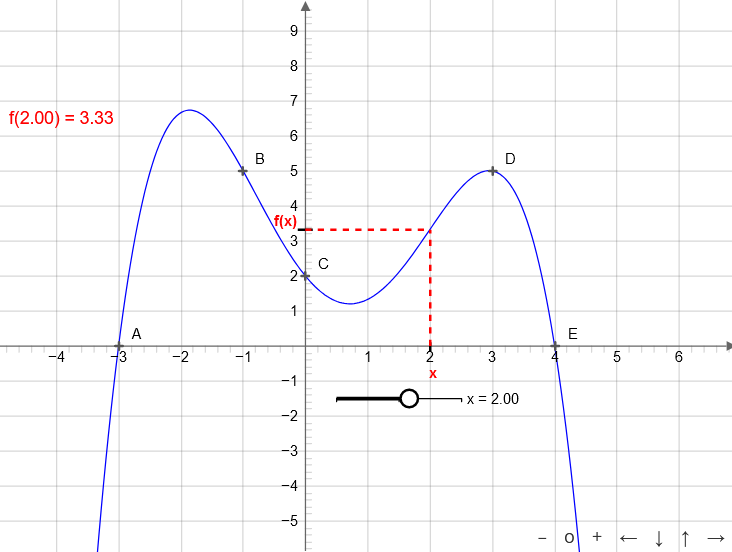
\includegraphics[width=\linewidth]{external/jsxgraph-algebra-function-notation.png}
\end{sbspanel}%
\begin{sbspanel}{0.21}%

\includegraphics[width=\linewidth]{generated/qrcode/sec-functions-readinggraphs-4.png}
\href{http://webwork.bridgew.edu/oer/functions_at_work/sec-functions-readinggraphs-4.html}{Standalone}%
\par
\href{http://webwork.bridgew.edu/oer/functions_at_work/sec-functions-readinggraphs-4-if.html}{Embed}%
\end{sbspanel}%
\end{sidebyside}%
\begin{example}{Example}{}{sec-functions-readinggraphs-5}%
Here is a static version of the interactive graphic above.%
\begin{image}{0}{1}{0}{}%
\resizebox{\linewidth}{!}{%
\begin{tikzpicture}
            [scale=0.5,
            declare function = {
              f(\x) =  0.0001*(\x-1)*(\x-4)*(\x-10)*(\x-20)*(\x-21)+3 ;
              xmin=0;
              xmax=22;
              ymin=0;
              ymax=10;
              pad=0.1;
              domainstart=-0.1;
              domainstop=22.1;
            }]
  \draw[axes] (0,ymin-pad)--(0,ymax+pad);
  \draw[axes] (xmin-pad,0)--(xmax+pad,0);
  \draw[grid] (xmin-pad,ymin-pad) grid (xmax+pad,ymax+pad);
  % Label x-axis
  %\foreach \i in {1,...,22}
  %  \node[below] at (\i,0) {$\i$};
  % Label y-axis
  %\foreach \i in {1,...,10}
  %  \node[left] at (0,\i) {$\i000$};

  % Graph the function defined in the TikZ environment
  \draw [curve,domain=domainstart:domainstop,smooth] plot ({\x},{f(\x)});

  \draw[color=red,dashed] (12.5,0) -- (12.5,{f(12.5)}) -- (0,{f(12.5)});
  \node[below,color=red] at (12.5,0) {$x$};
  \node[color=red] at (12.5-1,-0.5) {$\leftarrow$};
  \node[color=red] at (12.5+1,-0.5) {$\rightarrow$};
  \node[left,color=red] at (0,{f(12.5)}) {$f(x)$};
  \node[color=red] at (-1,{f(12.5)+1}) {$\Uparrow$};
  \node[color=red] at (-1,{f(12.5)-1}) {$\Downarrow$};
  \draw[fill=red,color=red] ({12.5},{f(12.5)}) circle (3pt);
  

\end{tikzpicture}
}%
\end{image}%
\end{example}
Reading graphs dynamically will play an essential role in the course, beginning in \hyperref[ch_limits]{Chapter~{\xreffont\ref{ch_limits}}}. But this skill also plays an important role in answering much more basic questions about graphs.%
\begin{exploration}{Exploration}{}{ex-reading_graphs}%
The graph of a function \(f\) is given below.%
\begin{image}{0.25}{0.5}{0.25}{}%
\resizebox{\linewidth}{!}{%
\begin{tikzpicture}
  \draw[grid,step=1] (-.6,-.4) grid (5.4,5.4);
  \draw[axes] (-1,0) -- (6,0);
  \draw[axes] (0,-1) -- (0,6) ;
        \foreach \x in {1,...,5}
          \draw (\x,.2) -- (\x,-.2)
        node[below right, font=\small] {\x};
        \foreach \y in {1,...,5}
          \draw (.2,\y) -- (-.2,\y)
        node[above left, font=\small] {\y};	
  \draw [curve,smooth,samples=100,domain=0:1] plot (\x,\x^2+1);
  \draw [curve,smooth,samples=100,domain=1:2] plot (\x,{2*(\x-1)+2});
  \draw [curve,smooth,samples=100,domain=2:4] plot (\x,{-2*(\x-2)+4});
  \draw [curve,smooth,samples=100,domain=4:5] plot (\x,{-2*(\x-5)^2+2});
  \draw [very thick, fill=black] (0,1) circle (2pt);
  \draw [very thick, fill=black] (5,2) circle (2pt);
  \node at (5.5,5.5) {$f(x)$};
\end{tikzpicture}
}%
\end{image}%
\begin{enumerate}[font=\bfseries,label=(\alph*),ref=\alph*]%
\item{}Compute \(f(0)\), \(f(2)\), \(f(4)\), and \(f(5)\).%
\par\smallskip%
\noindent\textbf{\blocktitlefont Answer}.\hypertarget{ex-reading_graphs-2-2}{}\quad{}\(f(0)=1\), \(f(2)=4\), \(f(4)=0\), and \(f(5)=2\)%
\item{}For what \(x\) is \(f(x)=2\)?  For what  \(x\) is \(f(x)=3\)? For what  \(x\) is \(f(x)=0\)?%
\par\smallskip%
\noindent\textbf{\blocktitlefont Answer}.\hypertarget{ex-reading_graphs-3-2}{}\quad{}\(f(x)=2\) when \(x=1\) or when \(x=3\) or when \(x=5\).%
\par
\(f(x)=3\) when \(x=1.5\) or when \(x=2.5\).%
\par
\(f(x)=0\) when \(x=4\).%
\par\smallskip%
\noindent\textbf{\blocktitlefont Solution}.\hypertarget{ex-reading_graphs-3-3}{}\quad{}\begin{image}{0.25}{0.5}{0.25}{}%
\resizebox{\linewidth}{!}{%
\begin{tikzpicture}
  \draw[grid] (-.6,-.4) grid (5.4,5.4);
  \draw[axes] (-1,0) -- (6,0);
  \draw[axes] (0,-1) -- (0,6) ;
        \foreach \x in {1,...,5}
          \draw (\x,.2) -- (\x,-.2)
        node[below right, font=\small] {\x};
        \foreach \y in {1,...,5}
          \draw (.2,\y) -- (-.2,\y)
        node[above left, font=\small] {\y};	
  \draw [curve,smooth,samples=100,domain=0:1] plot (\x,\x^2+1);
  \draw [curve,smooth,samples=100,domain=1:2] plot (\x,{2*(\x-1)+2});
  \draw [curve,smooth,samples=100,domain=2:4] plot (\x,{-2*(\x-2)+4});
  \draw [curve,smooth,samples=100,domain=4:5] plot (\x,{-2*(\x-5)^2+2});
  \draw [very thick, fill=black] (0,1) circle (2pt);
  \draw [very thick, fill=black] (5,2) circle (2pt);
    \draw [color=red, very thick] (5.4,3) -- (-0.6,3) node [left] {$f(x)=3$};
      \draw[color=red,fill] (1.5,3) circle (2pt);
      \draw[color=red,dashed,very thick] (1.5,3) -- (1.5,0);
      \draw[color=red,fill] (2.5,3) circle (2pt);
      \draw[color=red,dashed,very thick] (2.5,3) -- (2.5,0);
    \draw [color=blue, very thick] (5.4,2) -- (-0.6,2) node [left] {$f(x)=2$};
      \draw[color=blue,fill] (1,2) circle (2pt);
      \draw[color=blue,dashed,very thick] (1,2) -- (1,0);
      \draw[color=blue,fill] (3,2) circle (2pt);
      \draw[color=blue,dashed,very thick] (3,2) -- (3,0);
      \draw[color=blue,fill] (5,2) circle (2pt);
      \draw[color=blue,dashed,very thick] (5,2) -- (5,0);
      \draw[color=green,fill] (4,0) circle (2pt);
  \node at (5.5,5.5) {$f(x)$};
\end{tikzpicture}
}%
\end{image}%
Remember that the equation \(f(x)=2\) means that you are looking for the \emph{inputs} \(x\) which correspond to an \emph{output} of \(2\). Looking at the graph, we see that \(f(1)=2\) and that \(f(3)=2\) and that \(f(5)=2\).  That means that the solution set is \(x=1\ or\ x=3\ or\ x=5\).%
\begin{aside}{Aside}{}{ex-reading_graphs-3-3-3}%
\alert{Note:} Endpoints require special care. In this case, there was a \emph{filled in dot} at the point \((5,2)\), which means that \(f(5)\) is defined and equal to 2. If there was an \emph{open circle} at the point, then the function would be defined \emph{near} \(x=5\), but not \emph{at} \(x=5\).%
\end{aside}
Similarly, solving the equation \(f(x) = 3\) means finding the inputs \(x\) that correspond to an output (height) \(y\) of 3. Looking at the graph, we see that \(f(1.5)=3\) and \(f(2.5)=3\).  That means that the solutions set is \(x=1.5\ or\ x=2.5\)%
\par
Finally, solving \(f(x) = 0\) means finding the inputs \(x\) that have a height \(y\) of zero.  Looking at the graph, this happens only for \(x=4\).%
\item{}For what  \(x\) is \(f(x)\lt 2\)?%
\par\smallskip%
\noindent\textbf{\blocktitlefont Answer}.\hypertarget{ex-reading_graphs-4-2}{}\quad{}The output of the function is \emph{strictly less than} 2 on the set \([0,1)\bigcup(3,5)\), or equivalently when \(0\leq x\leq 1\ or\ 3\leq x\leq 5\).%
\par\smallskip%
\noindent\textbf{\blocktitlefont Solution}.\hypertarget{ex-reading_graphs-4-3}{}\quad{}\begin{image}{0.25}{0.5}{0.25}{}%
\resizebox{\linewidth}{!}{%
\begin{tikzpicture}
  \draw[grid] (-.6,-.4) grid (5.4,5.4);
  \draw[axes] (-1,0) -- (6,0);
  \draw[axes] (0,-1) -- (0,6) ;
        \foreach \x in {1,...,5}
          \draw (\x,.2) -- (\x,-.2)
        node[below right, font=\small] {\x};
        \foreach \y in {1,...,5}
          \draw (.2,\y) -- (-.2,\y)
        node[above left, font=\small] {\y};	
    
  \draw [color=blue, very thick] (3,2) -- (5,2);
  \draw [color=blue, very thick, dotted] (3,2)--(1,2);
  \draw [color=blue, very thick] (1,2) -- (0,2);
  %                    \draw[color=blue,dashed,very thick] (5,2) -- (5,0);
  %                    \draw[color=blue,dashed,very thick] (3,2) -- (3,0);
  %                    \draw[color=blue,dashed,very thick] (1,2) -- (1,0);
  \draw[color=blue,very thick,fill] (0,2) circle (3pt);
  \draw[color=blue,very thick,fill=white] (1,2) circle (3pt);
  \draw[color=blue,very thick,fill=white] (3,2) circle (3pt);
  \draw[color=blue,very thick,fill=white] (5,2) circle (3pt);

  \draw [curve,smooth,samples=100,domain=0:1] plot (\x,\x^2+1);
  \draw [curve,smooth,samples=100,domain=1:2] plot (\x,{2*(\x-1)+2});
  \draw [curve,smooth,samples=100,domain=2:4] plot (\x,{-2*(\x-2)+4});
  \draw [curve,smooth,samples=100,domain=4:5] plot (\x,{-2*(\x-5)^2+2});
  \draw [curve, fill=black] (0,1) circle (2pt);
  %                    \draw [color=black, very thick, fill=black] (5,2) circle (2pt);
  \node at (5.5,5.5) {$f(x)$};
\end{tikzpicture}
}%
\end{image}%
Remember that the equation \(f(x)\lt 2\) means that you are looking for the \emph{inputs} \(x\) which correspond to an output of \emph{strictly less than} \(2\). To understand this inequality, follow the graph of the function, moving through  \(x\)-values from left to right.%
\par
Above \(x=0\), the height is \(1\) which is less than \(2\). Moving right, the height of the function increases, but stays below \(2\) until we reach \(x=1\). That means that the function is \emph{less than} or \emph{equal to} 2 on the interval \([0,1]\). But because we want the height to be \emph{strictly less than} 2, we must exclude 1, giving us the interval \([0,1)\).%
\par
Similarly, the height is also less than 2 between \(x=3\) and \(x=5\), and equal to 2 at those endpoints, so the function is \emph{strictly less than} 2 on the interval \((3,5)\)%
\par
Putting it all together, we have that \(f(x)\lt 2\) on the set \([0,1)\bigcup (3,5)\), or equivalently when \(0\leq x\lt 1\ or\ 3\lt x\lt 5\).%
\item{}For what  \(x\) is \(f(x)\leq 3\)?%
\par\smallskip%
\noindent\textbf{\blocktitlefont Answer}.\hypertarget{ex-reading_graphs-5-2}{}\quad{}Remember that the equation \(f(x)\leq 2\) means that you are looking for the \emph{inputs} \(x\) which correspond to an output of \emph{less than} or \emph{equal to} \(3\). This happens for values of \(x\) satisfying \(0\leq x\leq 1.5\ or\ 2.5 \leq x\). In interval notation, this corresponds to the set \([0,1.5]\bigcup [2.5,5]\).%
\par\smallskip%
\noindent\textbf{\blocktitlefont Solution}.\hypertarget{ex-reading_graphs-5-3}{}\quad{}\begin{image}{0.25}{0.5}{0.25}{}%
\resizebox{\linewidth}{!}{%
\begin{tikzpicture}
  \draw[grid] (-.6,-.4) grid (5.4,5.4);
  \draw[axes] (-1,0) -- (6,0);
  \draw[axes] (0,-1) -- (0,6) ;
        \foreach \x in {1,...,5}
          \draw (\x,.2) -- (\x,-.2)
        node[below right, font=\small] {\x};
        \foreach \y in {1,...,5}
          \draw (.2,\y) -- (-.2,\y)
        node[above left, font=\small] {\y};	
    
  \draw [color=red, very thick] (2.5,3) -- (5,3);
  \draw [color=red, very thick, dotted] (1.5,3)-- (2.5,3);
  \draw [color=red, very thick] (1.5,3) -- (0,3);
  %                    \draw[color=red,dashed,very thick] (5,2) -- (5,0);
  %                    \draw[color=red,dashed,very thick] (3,2) -- (3,0);
  %                    \draw[color=red,dashed,very thick] (1,2) -- (1,0);
  \draw[color=red,very thick,fill] (0,3) circle (3pt);
  \draw[color=red,very thick,fill] (1.5,3) circle (3pt);
  \draw[color=red,very thick,fill] (2.5,3) circle (3pt);

  \draw [curve,smooth,samples=100,domain=0:1] plot (\x,\x^2+1);
  \draw [curve,smooth,samples=100,domain=1:2] plot (\x,{2*(\x-1)+2});
  \draw [curve,smooth,samples=100,domain=2:4] plot (\x,{-2*(\x-2)+4});
  \draw [curve,smooth,samples=100,domain=4:5] plot (\x,{-2*(\x-5)^2+2});
  \draw [color=black, very thick, fill=black] (0,1) circle (2pt);
  \draw [color=black, very thick, fill=black] (5,2) circle (2pt);
  \node at (5.5,5.5) {$f(x)$};
\end{tikzpicture}
}%
\end{image}%
\item{}For what  \(x\) is \(f(x)>0\)?%
\par\smallskip%
\noindent\textbf{\blocktitlefont Answer}.\hypertarget{ex-reading_graphs-6-2}{}\quad{}The inequality \(f(x)\gt 0\) is true for all inputs that correspond to an output that is strictly greater than 0. This is true for all values of \(x\) \emph{except} \(x=4\). So this is true for values of \(x\) in the interval \([0,4)\bigcup(4,5]\).%
\item{}What is the domain and range of \(f\)?%
\par\smallskip%
\noindent\textbf{\blocktitlefont Answer}.\hypertarget{ex-reading_graphs-7-2}{}\quad{}The domain of \(f(x)\) is the set of \(x\)-values where the function is defined.  In this example, the function is defined starting at \(x=0\) and stopping at \(x=5\). Therefore the domain is \([0,5]\).%
\par
The range of \(f(x)\) is the set of \(y\)-values that are output by the function.  Looking at the function, note that you can achieve outputs as small as \(f(x)=0\) (at \(x=4\)) and as large as \(f(x)=4\) (at \(x=2\)), as well as every output between those \(y\)-values. Furthermore, no larger or smaller \(y\) can be achieved.  As a result, the range of the function is the interval \([0,4]\).%
\end{enumerate}%
\end{exploration}%
\end{sectionptx}
\end{chapterptx}
 %
%
\typeout{************************************************}
\typeout{Chapter 2 Working with Functions}
\typeout{************************************************}
%
\begin{chapterptx}{Chapter}{Working with Functions}{}{Working with Functions}{}{}{ch-combiningfns}
\renewcommand*{\chaptername}{Chapter}
%
%
\typeout{************************************************}
\typeout{Section 2.1 Combining Functions}
\typeout{************************************************}
%
\begin{sectionptx}{Section}{Combining Functions}{}{Combining Functions}{}{}{sec-combining_functions}
The ``big idea'' behind all of algebra is the use of a symbols to represent a different object. The simplest thing you can do in algebra is to replace the symbol with the value it represents, often called ``plugging in''  the value.%
\begin{exploration}{Exploration}{}{ex-combiningfunctions1}%
Let \(f(x) = x^2 - 3x\).%
\begin{enumerate}[font=\bfseries,label=(\alph*),ref=\alph*]%
\item{}Evaluate \(f(5)\), and simplify completely.%
\par\smallskip%
\noindent\textbf{\blocktitlefont Solution}.\hypertarget{ex-combiningfunctions1-2-2}{}\quad{}The expression \(f(5)\) is really an instruction to take the definition of \(f(x) = x^2 - 3x\), and to replace every occurance of \(x\) with the value \(5\).  Performing this subsitution, and the simplifying, gives%
\begin{align*}
f(5) \amp= 5^2 - 3\cdot 5\\
\amp= 25 - 15\\
\amp= 10
\end{align*}
%
\item{}Evaluate \(f(5+h)\), and simplify completely.%
\par\smallskip%
\noindent\textbf{\blocktitlefont Solution}.\hypertarget{ex-combiningfunctions1-3-2}{}\quad{}Again, the expression \(f(5+h)\) is really an instruction to take the definition of \(f(x) = x^2 - 3x\), and to replace every occurance of \(x\) with the value \((5+h)\).  Performing this subsitution, gives the expression%
\begin{equation*}
f(5+h) = (5+h)^2 - 3\cdot (5+h)
\end{equation*}
It is \alert{very important} to include parentheses when you are subtituting \(x\) with the term \((5+h)\).%
\par
To simplify this expression, you should separately simplify the first term and the second term.  Expanding out (FOIL-ing) the first term gives%
\begin{equation*}
(5+h)^2 = (5+h)\cdot(5+h) = 5\cdot 5 + 5\cdot h + h\cdot 5 + h\cdot h = 25 + 10h +h^2\text{.}
\end{equation*}
Distributing out the second term gives%
\begin{equation*}
3\cdot (5+h) = 3\cdot 5 + 3\cdot h = 15 + 3h
\end{equation*}
Putting it all together we get%
\begin{align*}
f(5+h)   \amp=  (5+h)^2 - 3\cdot (5+h) \\
\amp= (25+10h+h^2) - (15+3h) \\
\amp= 25 + 10h + h^2 - 15 - 3h \\
\amp= 10 + 7h + h^2 
\end{align*}
\alert{Note:} Whenever substituing an expression into another expression, such as when we substitued the simplifications for \((5+h)^2\) and \(3\cdot (5+h)\) above, you must always include parentheses around each term.  Above, that helped us remember that we needed to distribute the subtraction to \emph{both} terms of \(15+3h\).%
\item{}Evaluate \(f(x^5)\), and simplify completely.%
\par\smallskip%
\noindent\textbf{\blocktitlefont Solution}.\hypertarget{ex-combiningfunctions1-4-2}{}\quad{}Again, the expression \(f(x^5)\) is really an instruction to take the definition of \(f(x) = x^2 - 3x\), and to replace every occurance of \(x\) with the value \(x^5\).  Performing this subsitution, gives the expression%
\begin{equation*}
f(x^5) = (x^5)^2 - 3\cdot (x^5)
\end{equation*}
We could separately simplify the first and second term as before, or we can do it all together in a single sequence of steps.  You can take whichever approach you are most comfortable with.%
\begin{align*}
f(x^5) \amp= (x^5)^2 - 3\cdot (x^5) \\
\amp= x^5 \cdot x^5 - 3 x^5 \\
\amp= x^{5+5} - 3x^5 \\
\amp= x^{10} - 3x^5 
\end{align*}
%
\end{enumerate}%
\end{exploration}%
Note that in our last example, we plugged a expression for x into another expression for x. In the language of \hyperref[ch-functions]{Chapter~{\xreffont\ref{ch-functions}}}, that means we plugged one function into another.  In mathematics, we call this process of plugging one function into another "composing" the functions.%
\begin{exploration}{Exploration}{}{ex-combiningfunctions2}%
Let \(f(x) = \dfrac{1}{x}\) and \(g(x) = x+5\).  Compute \(f\Big(g(x)\Big)\).%
\par\smallskip%
\noindent\textbf{\blocktitlefont Solution}.\hypertarget{ex-combiningfunctions2-2}{}\quad{}The problem asks us to evaluate the result of plugging the  function \(g(x)=x+5\) into the every occurance of \(x\) in the equation \(f(x) = \dfrac{1}{x}\)%
\par
First, we can look at \(f\Big(g(x)\Big)\), and notice that we have already been told  that the expression \(g(x)\) refers to \((x+5)\).  As a result, we can replace the argument to \(f\) as follows%
\begin{equation*}
f\Big(g(x)\Big)  = f\Big( x+5 \Big) 
\end{equation*}
%
\par
Next, we just replace every ocurance of \(x\) in the definition \(f(x) = \dfrac{1}{x}\) with the expression \((x+5)\).  This gives%
\begin{equation*}
f\Big(x+5\Big)  = \dfrac{1}{( x+5)} 
\end{equation*}
%
\par
Putting it all together, we get%
\begin{align*}
f\Big(g(x)\Big)  \amp= f\Big( x+5 \Big)  \\
\amp= \dfrac{1}{( x+5)}  
\end{align*}
%
\end{exploration}%
We'll need to do a lot of composition later in the semester. For now, we will use these concepts to practice our algebra skills.%
\begin{exploration}{Exploration}{}{ex-simplifyingfunctions1}%
Let \(f(x) = 3x^2 - x + 1\). Simplify the following expressions completely%
\begin{enumerate}[font=\bfseries,label=(\alph*),ref=\alph*]%
\item{}\(f(2)\)%
\par\smallskip%
\noindent\textbf{\blocktitlefont Solution}.\hypertarget{ex-simplifyingfunctions1-2-2}{}\quad{}\(f(2) = 3\cdot (2)^2 - (2) + 1 = 12 - 2 + 1 = 11\)%
\item{}\(f(2+h)\)%
\par\smallskip%
\noindent\textbf{\blocktitlefont Solution}.\hypertarget{ex-simplifyingfunctions1-3-2}{}\quad{}%
\begin{align*}
f(2+h) \amp = 3\cdot (2+h)^2 - (2+h) + 1\\
\amp = 3\cdot (2+h)\cdot (2 + h) - 2 - h + 1\\
\amp = 3\cdot (4 + 4h + h^2) - 2 - h + 1\\
\amp = 12 + 12h + 3h^2 - 2 - h + 1\\
\amp = 3h^2 + 11h + 11
\end{align*}
%
\item{}\(\dfrac{f(2+h)-f(2)}{h}\)%
\par\smallskip%
\noindent\textbf{\blocktitlefont Solution}.\hypertarget{ex-simplifyingfunctions1-4-2}{}\quad{}This expression is slightly more complex.  The key idea is to realize that the numerator contains two \emph{separate} expressions \(f(2+h)\) and \(f(2)\), and that we have already found that they equal \((3h^2+11h+11)\) and \((11)\) respectively.  Making the appropriate replacements gives%
\begin{equation*}
\dfrac{f(2+h)-f(2)}{h} = \dfrac{(3h^2+11h+11)-(11)}{h}
\end{equation*}
Now we can use basic algebra to simplify the expression as before.%
\begin{align*}
\amp = \dfrac{3h^2+11h}{h}\\
\amp = \dfrac{h(3h+11)}{h}\\
\amp = \dfrac{h}{h}\cdot \dfrac{3h+11}{1}\\
\amp = 3h+11
\end{align*}
%
\end{enumerate}%
\end{exploration}%
The previous example is complicated because it combines a number of different kinds of steps. To see what's going on, it can help to think of these different steps separately.%
\begin{exploration}{Exploration}{}{ex-combiningfunctions3}%
Let \(f(x) = 2x^2-4x\) and \(g(x)=2x-4\).  Simplify the following expressions completely.%
\begin{enumerate}[font=\bfseries,label=(\alph*),ref=\alph*]%
\item{}\(f(x)+g(x)\)%
\par\smallskip%
\noindent\textbf{\blocktitlefont Solution}.\hypertarget{ex-combiningfunctions3-2-2}{}\quad{}To evaluate the expression \(f(x)+g(x)\), first replace \(f(x)\) with the expression \((2x^2-4x)\), and replace \(g(x)\) with the expression \((2x-4)\).  Then, simplify the remaining expression completely using algebra.%
\begin{align*}
f(x)+g(x)\amp =(2x^2-4x) + (2x-4)\\
\amp = 2x^2-4x + 2x - 4\\
\amp = 2x^2 -2x -4 
\end{align*}
%
\item{}\(f(x)-g(x)\)%
\par\smallskip%
\noindent\textbf{\blocktitlefont Solution}.\hypertarget{ex-combiningfunctions3-3-2}{}\quad{}To evaluate the expression \(f(x)-g(x)\), first replace \(f(x)\) with the expression \((2x^2-4x)\), and replace \(g(x)\) with the expression \((2x-4)\).  Then, simplify the remaining expression completely using algebra.%
\begin{align*}
f(x)+g(x)\amp =(2x^2-4x) - (2x-4)\\
\amp = 2x^2-4x - 2x + 4\\
\amp = 2x^2 -6x + 4
\end{align*}
Note that subtracting both terms of \(2x-4\) was the same thing as adding \(-2x\) and adding a positive \(4x\)%
\item{}\(f(x)\cdot g(x)\)%
\par\smallskip%
\noindent\textbf{\blocktitlefont Solution}.\hypertarget{ex-combiningfunctions3-4-2}{}\quad{}To evaluate the expression \(f(x)\cdot g(x)\), first replace \(f(x)\) with the expression \((2x^2-4x)\), and replace \(g(x)\) with the expression \((2x-4)\).  Then, simplify the remaining expression completely using algebra.%
\begin{align*}
f(x)\cdot g(x)\amp =(2x^2-4x) \cdot (2x-4)\\
\amp = 2x^2\cdot 2x + 2x^2 \cdot (-4) + (-4x)\cdot 2x + (-4x)\cdot (-4) \\
\amp = 4x^3 - 8x^2 - 8x^2 + 16x\\
\amp = 4x^3 - 16x^2 + 16x
\end{align*}
%
\item{}\(\dfrac{f(x)}{g(x)}\)%
\par\smallskip%
\noindent\textbf{\blocktitlefont Solution}.\hypertarget{ex-combiningfunctions3-5-2}{}\quad{}To evaluate the expression \(\dfrac{f(x)}{g(x)}\), first replace \(f(x)\) with the expression \((2x^2-4x)\), and replace \(g(x)\) with the expression \((2x-4)\).  Then, simplify the remaining expression completely using algebra.%
\par
%
\begin{align*}
\dfrac{f(x)}{g(x)} \amp = \dfrac{(2x^2-4x)}{(2x-4)} 
\end{align*}
The only way to simplify a fraction is to factor the top and bottom separately, and see if any of the terms cancel.  The top factors as \(2x^2-4x = 2\cdot(x^2-2x) = 2\cdot x\cdot (x-2)\).  The bottom factors as \(2x-4= 2 \cdot (x-2)\).  Using this, we get%
\begin{align*}
\dfrac{f(x)}{g(x)} \amp = \dfrac{(2x^2-4x)}{(2x-4)} \\
\amp = \dfrac{2\cdot x\cdot (x-2)}{2\cdot (x-2)}\\
\amp = \dfrac{x}{1}\\
\amp = x
\end{align*}
Surprisingly, the expression \(\dfrac{f(x)}{g(x)}\) simplifies down to the identifty function \(\dfrac{f(x)}{g(x)} = x\)%
\item{}\(f\Big(g(x)\Big)\)%
\par\smallskip%
\noindent\textbf{\blocktitlefont Solution}.\hypertarget{ex-combiningfunctions3-6-2}{}\quad{}To evaluate the expression \(f\Big(g(x)\Big)\), first replace \(g(x)\) with teh expression \((2x-4)\).  This gives%
\begin{equation*}
f\Big(g(x)\Big) = f\Big(2x-4\Big)
\end{equation*}
But the expression \(f(2x-4)\) is just the instruction to take the equation \(f(x) = 2x^2-4x\), and to replace each copy of \(x\) with the expression \((2x-4)\). This gives%
\begin{equation*}
f(2x-4) = 2(2x-4)^2 - 4(2x-4)\text{.}
\end{equation*}
Simplifying this gives%
\begin{align*}
f\Big(g(x)\Big) \amp = f\Big(2x-4\Big) \\
\amp = 2(2x-4)^2 - 4(2x-4)\\
\amp = 2(2x-4)(2x-4) - 4(2x-4)\\
\amp = 2(4x^2-16x+16) - 8x + 16\\
\amp = 8x^2 -32x + 32 - 8x + 16\\
\amp = 8x^2 - 40x + 48 
\end{align*}
%
\end{enumerate}%
\end{exploration}%
In the examples above, we have seen how to simplify various combinations of functions algebraically.%
\par
For a few ways of combining of functions, it is also possible to explain very precisely how the combination changes the graph of the function. Let \(y = f(x)\) be the graph of some function, and let \(a,b,c,d\) be constant numbers.%
\begin{itemize}[label=\textbullet]
\item{}The graph of \(y = a\cdot f(x)\) is obtained by scaling the graph of \(y=f(x)\) by \(a\).%
\item{}The graph of \(y = f(x + b)\) is obtained by scaling the graph of \(y=f(x)\) left \(b\) units when \(b\) is positive (and right when \(b\) is negative).%
\item{}The graph of \(y = f(x) + c\) is obtained by shifting the graph of \(y=f(x)\) up by \(c\) units when \(c\) is positive (and down when \(c\) is negative).%
\end{itemize}
%
\end{sectionptx}
%
%
\typeout{************************************************}
\typeout{Section 2.2 \textasteriskcentered{}Graphs of Totals and Changes}
\typeout{************************************************}
%
\begin{sectionptx}{Section}{\textasteriskcentered{}Graphs of Totals and Changes}{}{\textasteriskcentered{}Graphs of Totals and Changes}{}{}{sec_graphsoftotalsandchanges}
Many things change over time, such as the cost of gasoline. There are different ways of thinking about describing this change. For example, suppose the price of gas over the course of a single week is given by the following table:%
\begin{equation*}
\begin{array}{c|c|c|c|c|c|c|c}
\text{day }(x)         
&  1 
&  2   
&  3  
&  4  
&  5 
&  6 
&  7  
\\ \hline
\text{cost of gas }(y) 
& 4  
& 3.75
& 3.25
& 3.75
& 2  
& 2.5
& 3
\end{array}
\end{equation*}
%
\par
This gives us the \terminology{total} cost of gas per day. There are also another way to think about this: how much does the price change each day? Over the course of the week the price decreases 25 cents, then decreases another 50 cents, then increases 50 cents, then increases \(\$1.25\), then decreases \(\$2.50\), and finally increases another 50 cents.%
\par
We will write \(\Delta y\) to emphasize that this is the \terminology{change} in price each day in a table.%
\begin{equation*}
\begin{array}{c|c|c|c|c|c|c|c}
\text{day }(x)
&  1 
&  2   
&  3  
&  4  
&  5 
&  6 
&  7  
\\ \hline
\text{change in gas }(\Delta y) 
& N/A  
& -0.25 
& -0.50 
&  0.50 
& -1.75 
&  0.50 
&  0.50
\end{array}
\end{equation*}
%
\begin{example}{Example}{A Strategy for Computing \(\Delta y\).}{sec_graphsoftotalsandchanges-5}%
In the example above, we described the change in words, and summarized this in a table. But we can also find the change \(\Delta y\) using mathematical language.%
\par
Day 1 is a special case. Because it is our first data point, there's nothing to compare it to.%
\par
On day 2 our cost \(y\) was 3.75, and on day 1 our cost \(y\) was 4. Then the \terminology{change in y on day 2} is \(\Delta y = (3.75) - (4) = -0.25\). We can also translate this into function language.%
\begin{itemize}[label=\textbullet]
\item{}The cost on day 1 is \textdollar{}4, so we write \(f(1) = 4\)%
\item{}The cost on day 2 is \textdollar{}3.75, so we write \(f(2) = 3.75\)%
\item{}To compute \(\Delta y\) on day 2, we compute \(\Delta y = f(2)-f(1) = 3.75-4.00=-0.25\)%
\end{itemize}
Repeating this process, we can find \(\Delta y\) for days 3, 4, 5, 6, and 7.%
\par
We can also summarize this technique using even more general mathemaitcal language by defining the \alert{change in \(y\)} due to \alert{changing from \(x_1\) to \(x_2\)} to be the expression%
\begin{equation*}
\Delta y = f(x_2) - f(x_1)
\end{equation*}
%
\end{example}
Now we have two tables, which \emph{both give functions} that describe a different perspective on how the cost of gas changes over time: the total value (\(y\)) of gas graphed with respect to time, and the change in value (\(\Delta y\)) graphed with respect to time.%
\par
To see how they're related, we can graph both functions side by side:%
\begin{image}{0}{1}{0}{}%
\resizebox{\linewidth}{!}{%
                    %%%% EXAMPLE 1 %%%%
                    %\def \tikzhistogram (#1,#2){	\draw[draw=black,thick,fill=blue,opacity=0.65] (#1,#2) rectangle ({#1-1},0) ;}
                    \def \tikzhistogram (#1,#2){\draw[fill=blue,opacity=0.3] ({#1+0.45},#2) rectangle ({#1-0.45},0); \draw[draw,thick] ({#1+0.45},#2) rectangle ({#1-0.45},0); \node[draw,fill=blue, circle,inner sep=2pt] at (#1,#2) {};}
                    \def \xmin {0}
                    \def \xmax {7}
                    \def \xunits {day}
                    \def \yunits {cost}
                    \def \dyunits{change in cost}
                    %% Information about the total (y) graph
                    \def \ymin {0}								%% First height to be be drawn with dashed lines
                    \def \ysecondmajoraxis {1}		%% Second height to be be drawn with dashed lines
                    \def \yfirstminoraxis  {0.5}	%% First line to be drawn with dotted lines
                    \def \ysecondminoraxis {1.5}	%% Second lin eto be drawn with dotted lines
                    \def \ymax {6}
                    %% Information about the change (\Delta y) graph
                    \def \dymin {-3}
                    \def \dysecondmajoraxis {-2}
                    \def \dyfirstminoraxis  {-2.5}
                    \def \dysecondminoraxis {-1.5}
                    \def \dymax {3}
                    \def \xscale {0.8*0.8}
                    \def \dyscale {0.6}
                    \begin{tikzpicture}[xscale=\xscale,yscale=\dyscale]
                        %% Graph of Total %%
                        %\draw ({\xmin-1},{\ymin-1}) rectangle ({\xmax+1.5},{\ymax+1.25});
                        \node at ({(\xmin+\xmax)/2},{\ymin-1.75}) {Graph of Total \ $y$};
                        %
                        %% Draw horizontal lines at major and minor y-values
                        \foreach \i in {\ymin,\ysecondmajoraxis,...,\ymax}
                            \draw[major gridlines] (\xmin,\i)--({\xmax+1},\i);
                        \foreach \i in {\yfirstminoraxis,\ysecondminoraxis,...,\ymax}
                            \draw[minor gridlines] (\xmin,\i)--({\xmax+1},\i);
                        %
                        %% Draw and label x and y axes
                        \draw[axes,-latex] ({\xmin},0) -- ({\xmax+1},0) node [below] {\xunits};
                        \draw[axes,-latex] (0,{\ymin}) -- (0,{\ymax+0.5}) node [above right] {\yunits};
                        \foreach \i in {1,...,\xmax}
                            \node[below,fill=white,yshift=-2pt] at (\i, 0) {\small $\i$};
                        \foreach \i in {\ymin,...,\ymax}
                            \node[left,fill=white,xshift=-2pt] at (0,\i) {\small $\i$};
                        
                        \foreach \i in {1,...,\xmax}
                            \draw[vertical gridlines] (\i, {\ymin}) -- (\i, {\ymax+0.25});
                        
                        %\draw[draw=black,thick,fill=blue,opacity=0.75] (1,4) rectangle ({1-1},0);
                            
                        \tikzhistogram(1,4);
                        \tikzhistogram(2,3.75);
                        \tikzhistogram(3,3.25);
                        \tikzhistogram(4,3.75);
                        \tikzhistogram(5,2);
                        \tikzhistogram(6,2.5);
                        \tikzhistogram(7,3);
                        
                    \end{tikzpicture}

                    %%%% END EXAMPLE 1 %%%% 
                    %\def \tikzhistogram (#1,#2){	\draw[draw=black,thick,fill=blue,opacity=0.65] (#1,#2) rectangle ({#1-1},0) ;}
                    \def \tikzhistogram (#1,#2){\draw[fill=blue,opacity=0.3] ({#1+0.45},#2) rectangle ({#1-0.45},0); \draw[draw,thick] ({#1+0.45},#2) rectangle ({#1-0.45},0); \node[draw,fill=blue, circle,inner sep=2pt] at (#1,#2) {};}
                    \def \xmin {0}
                    \def \xmax {7}
                    \def \xunits {day}
                    \def \yunits {cost}
                    \def \dyunits{change in cost}
                    %% Information about the total (y) graph
                    \def \ymin {0}								%% First height to be be drawn with dashed lines
                    \def \ysecondmajoraxis {1}		%% Second height to be be drawn with dashed lines
                    \def \yfirstminoraxis  {0.5}	%% First line to be drawn with dotted lines
                    \def \ysecondminoraxis {1.5}	%% Second lin eto be drawn with dotted lines
                    \def \ymax {6}
                    %% Information about the change (\Delta y) graph
                    \def \dymin {-3}
                    \def \dysecondmajoraxis {-2}
                    \def \dyfirstminoraxis  {-2.5}
                    \def \dysecondminoraxis {-1.5}
                    \def \dymax {3}
                    \def \xscale {0.8*0.8}
                    \def \dyscale {0.6}
                    \begin{tikzpicture}[xscale=\xscale,yscale=\dyscale]
                        %% Graph of Change %%
                        %\draw ({\xmin-1.5},{\dymin-1}) rectangle ({\xmax+1.5},{\dymax+1.25});
                        \node at ({(\xmin+\xmax)/2},{\dymin-1.75}) {Graph of Change \ $\Delta y$};
                        %
                        %% Draw horizontal lines at major and minor y-values
                        \foreach \i in {\dymin,\dysecondmajoraxis,...,\dymax}
                            \draw[major gridlines] (\xmin,\i)--({\xmax+1},\i);
                        \foreach \i in {\dyfirstminoraxis,\dysecondminoraxis,...,\dymax}
                            \draw[minor gridlines] (\xmin,\i)--({\xmax+1},\i);
                        %
                        %% Draw and label x and y axes
                        \draw[axes,-latex] ({\xmin},0) -- ({\xmax+1},0) node [below] {\xunits};
                        \draw[axes,latex-latex] (0,{\dymin-0.5}) -- (0,{\dymax+0.5})  node[above right]{\dyunits};
                        \foreach \i in {1,...,\xmax}
                            \node[below,fill=white,yshift=-6pt] at (\i, \dymin) {\small $\i$};
                        \foreach \i in {\dymin,...,\dymax}
                            \node[left,fill=white,xshift=-2pt] at (0,\i) {\small $\i$};
                        
                        \foreach \i in {1,...,\xmax}
                            \draw[vertical gridlines] (\i, {\dymin-0.25}) -- (\i, {\dymax+0.25});
                        
                        
                        %\tikzhistogram(1,0);
                        \tikzhistogram(2,-.25);
                        \tikzhistogram(3,-.5);
                        \tikzhistogram(4,.5);
                        \tikzhistogram(5,-1.75);
                        \tikzhistogram(6,.5);
                        \tikzhistogram(7,.5);
                        
                    \end{tikzpicture}
                    %%%% END EXAMPLE 1 %%%%
}%
\end{image}%
In the example above, the biggest drop in the total \(y\) (left) occurs on day 5.  This matches the graph on the right, where day 5 has the largest negative movement (change) \(\Delta y\). On the other hand, there is almost no change on day 2 in the total graph on the left (only a small drop in \(y\)), which matches the small value of \(\Delta y\) in the change graph on the right.%
\par
Graphs of totals and changes occur in a wide variety of economic, business, and other contexts. But one of the most common and important applications is in the important distinction between \emph{debts} and \emph{deficits}.%
\begin{paragraphs}{Debts and Deficits.}{economics-debts-and-deficits}%
The \terminology{US national debt} in a given year is the total amount of money that the government owed in that year. The \terminology{net revenue} from a given year is the difference between money taken in (through taxes) and money spent by the government. The government is running an \terminology{annual deficit} if it spends more than it takes in. In other words, having negative net revenue in a given year is the same thing as a positive deficit in that year.%
\par
The page \href{https://datalab.usaspending.gov/americas-finance-guide/deficit/trends/}{https:\slash{}\slash{}datalab.usaspending.gov\slash{}americas-finance-guide\slash{}deficit\slash{}trends\slash{}}\footnote{\nolinkurl{datalab.usaspending.gov/americas-finance-guide/deficit/trends/}\label{economics-debts-and-deficits-3-2}} lists US budget deficits in \emph{trillions of dollars} since the year 2000, rounded to two decimal places. The same page indicates that the US debt in 2000 was 5.65 trillions.%
\par
As before, we can compute the debt \(y\) for each year since 2000 by starting with 5.65 and repeatedly adding the \(\Delta y\) for each year. \footnote{\terminology{Note:} Actually, the debt is always more than the sum of the deficits, since the government must also pay \terminology{interest} on the money it borrows to cover a deficit. The true debt for each year is shown using a red dot. The actual value of the debt (not adjusted for inflation) can be found at \href{https://fiscaldata.treasury.gov/datasets/debt-to-the-penny/debt-to-the-penny}{\nolinkurl{https://fiscaldata.treasury.gov/datasets/debt-to-the-penny/debt-to-the-penny}}.\label{economics-debts-and-deficits-4-3}} This gives us our familiar graphs of the total \(y\) and change \(\Delta y\).%
\begin{image}{0}{1}{0}{}%
\resizebox{\linewidth}{!}{%
                    %%%% EXAMPLE DEBT/DEFICIT %%%%
                    %\def \tikzhistogram (#1,#2){	\draw[draw=black,thick,fill=blue,opacity=0.65] (#1,#2) rectangle ({#1-1},0) ;}
                    \def \tikzhistogram (#1,#2){	\draw[fill=blue,opacity=0.6] ({#1+0.4},#2) rectangle ({#1-0.4},0) ; \draw[draw=black] ({#1+0.4},#2) rectangle ({#1-0.4},0) ; \node[draw,fill=blue, circle,inner sep=1	pt] at (#1,#2) {}; }
                    \def \reddot (#1,#2){ \node [draw,circle,fill=red,inner sep=2pt] at (#1,#2) {}; }
                    \def \debtyscale {0.45} % Full page graph with yscale of 0.7 
                    \def \xmin {0}
                    \def \xmax {23}
                    \def \xunits {year}
                    \def \yunits {debt}
                    \def \dyunits{deficit}
                    %% Information about the total (y) graph
                    \def \ymin {0}								%% First height to be be drawn with dashed lines
                    \def \ysecondmajoraxis {5}		%% Second height to be be drawn with dashed lines
                    \def \yfirstminoraxis  {1}	%% First line to be drawn with dotted lines
                    \def \ysecondminoraxis {2}	%% Second lin eto be drawn with dotted lines
                    \def \ymax {32}
                    %% Information about the change (\Delta y) graph
                    \def \dymin {-1}
                    \def \dysecondmajoraxis {-0}
                    \def \dyfirstminoraxis  {-0.5}
                    \def \dysecondminoraxis {0.5}
                    \def \dymax {3.5}

                    \def \xscale{0.35*0.8}

                    \hspace{-1.25cm}
                    \begin{tikzpicture}[xscale=\xscale,yscale=\debtyscale]
                        %% Graph of Total %%
                        %\draw ({\xmin-1},{\ymin-1}) rectangle ({\xmax+1.5},{\ymax+1.25});
                        \node at ({(\xmin+\xmax)/2},{\ymin-1.25}) {Graph of total \ $y$ (debt)};
                        %
                        %% Draw horizontal lines at major and minor y-values
                        \foreach \i in {\ymin,\ysecondmajoraxis,...,\ymax}
                            \draw[major gridlines] (\xmin,\i)--({\xmax+1},\i);
                        %\foreach \i in {\yfirstminoraxis,\ysecondminoraxis,...,\ymax}
                            %\draw[minor gridlines] (\xmin,\i)--({\xmax+1},\i);
                        %
                        %% Draw and label x and y axes
                        \draw[axes,-latex] ({\xmin},0) -- ({\xmax+1},0) node [right] {\xunits};
                        \draw[axes,-latex] (0,{\ymin}) -- (0,{\ymax+0.5}) node [above,fill=white] {\yunits};
                        %\foreach \i in {1,...,\xmax}
                            %\node[below,yshift=-2pt] at (\i, 0) {\small $\i$};
                        \node[below,yshift=-2pt] at (1, 0) {\tiny $2000$};
                        \node[below,yshift=-2pt] at (21, 0) {\tiny $2020$};
                        \foreach \i in {\ymin,\yfirstminoraxis,...,\ymax}
                            \node[left,xshift=-2pt] at (0,\i) {\small $\i$};
                        
                        \foreach \i in {1,...,\xmax}
                            \draw[vertical gridlines] (\i, {\ymin}) -- (\i, {\ymax+0.25});
                        
                        %\draw[draw=black,thick,fill=blue,opacity=0.75] (1,4) rectangle ({1-1},0);
                            
                        \tikzhistogram(1+0,5.66);
                        \tikzhistogram(1+1,5.53);
                        \tikzhistogram(1+2,5.69);
                        \tikzhistogram(1+3,6.06);
                        \tikzhistogram(1+4,6.47);
                        \tikzhistogram(1+5,6.79);
                        \tikzhistogram(1+6,7.04);
                        \tikzhistogram(1+7,7.20);
                        \tikzhistogram(1+8,7.65);
                        \tikzhistogram(1+9,9.07);
                        \tikzhistogram(1+10,10.36);
                        \tikzhistogram(1+11,11.66);
                        \tikzhistogram(1+12,12.75);
                        \tikzhistogram(1+13,13.43);
                        \tikzhistogram(1+14,13.91);
                        \tikzhistogram(1+15,14.35);
                        \tikzhistogram(1+16,14.94);
                        \tikzhistogram(1+17,15.61);
                        \tikzhistogram(1+18,16.39);
                        \tikzhistogram(1+19,17.37);
                        \tikzhistogram(1+20,20.50);
                        \tikzhistogram(1+21,23.27);
            \tikzhistogram(1+22,24.65);
                        
                        \reddot(1+0,5.66);
                        \reddot(1+1,5.81);
                        \reddot(1+2,6.23);
                        \reddot(1+3,6.78);
                        \reddot(1+4,7.38);
                        \reddot(1+5,7.93);
                        \reddot(1+6,8.51);
                        \reddot(1+7,9.01);
                        \reddot(1+8,10.02);
                        \reddot(1+9,11.91);
                        \reddot(1+10,13.56);
                        \reddot(1+11,14.79);
                        \reddot(1+12,16.07);
                        \reddot(1+13,16.74);
                        \reddot(1+14,17.82);
                        \reddot(1+15,18.15);
                        \reddot(1+16,19.57);
                        \reddot(1+17,20.24);
                        \reddot(1+18,21.52);
                        \reddot(1+19,22.72);
                        \reddot(1+20,26.95);
                        \reddot(1+21,28.91);
                        \reddot(1+22,31.33);

                    \end{tikzpicture}
                    %
                    \quad
                    %
                    \begin{tikzpicture}[baseline=-5cm,xscale=\xscale,yscale=\debtyscale]
                        %\node (O) at (0,0) {};
                        %% Graph of Change %%
                        %\draw ({\xmin-1.5},{\dymin-1}) rectangle ({\xmax+1.5},{\dymax+1.25});
                        \node at ({(\xmin+\xmax)/2},{\dymin-1.25}) {Graph of change \ $\Delta y$ (deficit)};
                        %
                        %% Draw horizontal lines at major and minor y-values
                        \foreach \i in {\dymin,\dysecondmajoraxis,...,\dymax}
                            \draw[major gridlines] (\xmin,\i)--({\xmax+1},\i);
                        \foreach \i in {\dyfirstminoraxis,\dysecondminoraxis,...,\dymax}
                            \draw[minor gridlines] (\xmin,\i)--({\xmax+1},\i);
                        %
                        %% Draw and label x and y axes
                        \draw[axes,-latex] ({\xmin},0) -- ({\xmax+1},0) node [right] {\xunits};
                        \draw[axes,latex-latex] (0,{\dymin-0.5}) -- (0,{\dymax+0.5})  node[above]{\dyunits};
                        %\foreach \i in {1,...,\xmax}
                            %\node[below,fill=white,yshift=-6pt] at (\i, \dymin) {\small $\i$};
                        \node[below,yshift=-2pt] at (1, \dymin) {\tiny $2000$};
                        \node[below,yshift=-2pt] at (21, \dymin) {\tiny $2020$};
                        \foreach \i in {\dymin,...,\dymax}
                            \node[left,xshift=-2pt] at (0,\i) {\small $\i$};
                        
                        \foreach \i in {1,...,\xmax}
                            \draw[vertical gridlines] (\i, {\dymin-0.25}) -- (\i, {\dymax+0.25});
                        
                        \tikzhistogram(1+0,-0.24);
                        \tikzhistogram(1+1,-0.13);
                        \tikzhistogram(1+2,0.16);
                        \tikzhistogram(1+3,0.37);
                        \tikzhistogram(1+4,0.41);
                        \tikzhistogram(1+5,0.32);
                        \tikzhistogram(1+6,0.25);
                        \tikzhistogram(1+7,0.16);
                        \tikzhistogram(1+8,0.45);
                        \tikzhistogram(1+9,1.42);
                        \tikzhistogram(1+10,1.29);
                        \tikzhistogram(1+11,1.3);
                        \tikzhistogram(1+12,1.09);
                        \tikzhistogram(1+13,0.68);
                        \tikzhistogram(1+14,0.48);
                        \tikzhistogram(1+15,0.44);
                        \tikzhistogram(1+16,0.59);
                        \tikzhistogram(1+17,0.67);
                        \tikzhistogram(1+18,0.78);
                        \tikzhistogram(1+19,0.98);
                        \tikzhistogram(1+20,3.13);
                        \tikzhistogram(1+21,2.77);
                        \tikzhistogram(1+22,1.38);
                    \end{tikzpicture}
                    %%%% END EXAMPLE DEBT/DEFICIT %%%%
}%
\end{image}%
\end{paragraphs}%
\par\medskip
In most examples, we will only be given one of these types of graphs, and we will need to create the other type of graph. In the next example you are only given the graph of the total value (\(y\)), and asked to find the graph of the change (\(\Delta y\)).%
\begin{exploration}{Exploration}{Using Total Value to Compute Change.}{ex-using-total-value-to-compute-change}%
The graph of gas price as a function of the day \(x\) is given below on the left.%
\begin{image}{0}{1}{0}{}%
\resizebox{\linewidth}{!}{%
            %%%% EXAMPLE 2 %%%%
            %\def \tikzhistogram (#1,#2){	\draw[draw=black,thick,fill=blue,opacity=0.65] (#1,#2) rectangle ({#1-1},0) ;}
            \def \tikzhistogram (#1,#2){\draw[fill=blue,opacity=0.3] ({#1+0.45},#2) rectangle ({#1-0.45},0); \draw[draw,thick] ({#1+0.45},#2) rectangle ({#1-0.45},0); \node[draw,fill=blue, circle,inner sep=2pt] at (#1,#2) {};}
            \def \xmin {0}
            \def \xmax {7}
            \def \xunits {day}
            \def \yunits {cost}
            \def \dyunits{change in cost}
            %% Information about the total (y) graph
            \def \ymin {0}								%% First height to be be drawn with dashed lines
            \def \ysecondmajoraxis {1}		%% Second height to be be drawn with dashed lines
            \def \yfirstminoraxis  {0.5}	%% First line to be drawn with dotted lines
            \def \ysecondminoraxis {1.5}	%% Second lin eto be drawn with dotted lines
            \def \ymax {6}
            %% Information about the change (\Delta y) graph
            \def \dymin {-3}
            \def \dysecondmajoraxis {-2}
            \def \dyfirstminoraxis  {-2.5}
            \def \dysecondminoraxis {-1.5}
            \def \dymax {3}
            \def \xscale{0.8*0.8}
            \def \yscale{0.8}

            \begin{tikzpicture}[xscale=\xscale,yscale=\yscale]
              %% Graph of Total %%
              \draw ({\xmin-1},{\ymin-1}) rectangle ({\xmax+1.5},{\ymax+1.25});
              \node at ({(\xmin+\xmax)/2},{\ymin-1.75}) {Graph of Total \ $y$};
              %
              %% Draw horizontal lines at major and minor y-values
              \foreach \i in {\ymin,\ysecondmajoraxis,...,\ymax}
                \draw[major gridlines] (\xmin,\i)--({\xmax+1},\i);
              \foreach \i in {\yfirstminoraxis,\ysecondminoraxis,...,\ymax}
                \draw[minor gridlines] (\xmin,\i)--({\xmax+1},\i);
              %
              %% Draw and label x and y axes
              \draw[axes,-latex] ({\xmin},0) -- ({\xmax+1},0) node [below] {\xunits};
              \draw[axes,-latex] (0,{\ymin}) -- (0,{\ymax+0.5}) node [above right] {\yunits};
              \foreach \i in {1,...,\xmax}
                \node[below,fill=white,yshift=-2pt] at (\i, 0) {\small $\i$};
              \foreach \i in {\ymin,...,\ymax}
                \node[left,fill=white,xshift=-2pt] at (0,\i) {\small $\i$};
              
              \foreach \i in {1,...,\xmax}
                \draw[vertical gridlines] (\i, {\ymin}) -- (\i, {\ymax+0.25});
              
              %\draw[draw=black,thick,fill=blue,opacity=0.75] (1,4) rectangle ({1-1},0);
                
              \tikzhistogram(1,2);
              \tikzhistogram(2,3.5);
              \tikzhistogram(3,4);
              \tikzhistogram(4,3);
              \tikzhistogram(5,4.5);
              \tikzhistogram(6,2);
              \tikzhistogram(7,3.5);
              
            \end{tikzpicture}
            %
            \quad
            %
            \begin{tikzpicture}[xscale=\xscale,yscale=\yscale]
              %% Graph of Change %%
              \draw ({\xmin-1.5},{\dymin-1}) rectangle ({\xmax+1.5},{\dymax+1.25});
              \node at ({(\xmin+\xmax)/2},{\dymin-1.75}) {Graph of Change \ $\Delta y$};
              %
              %% Draw horizontal lines at major and minor y-values
              \foreach \i in {\dymin,\dysecondmajoraxis,...,\dymax}
                \draw[major gridlines] (\xmin,\i)--({\xmax+1},\i);
              \foreach \i in {\dyfirstminoraxis,\dysecondminoraxis,...,\dymax}
                \draw[minor gridlines] (\xmin,\i)--({\xmax+1},\i);
              %
              %% Draw and label x and y axes
              \draw[axes,-latex] ({\xmin},0) -- ({\xmax+1},0) node [below] {\xunits};
              \draw[axes,latex-latex] (0,{\dymin-0.5}) -- (0,{\dymax+0.5})  node[above right]{\dyunits};
              \foreach \i in {1,...,\xmax}
                \node[below,fill=white,yshift=-6pt] at (\i, \dymin) {\small $\i$};
              \foreach \i in {\dymin,...,\dymax}
                \node[left,fill=white,xshift=-2pt] at (0,\i) {\small $\i$};
              
              \foreach \i in {1,...,\xmax}
                \draw[vertical gridlines] (\i, {\dymin-0.25}) -- (\i, {\dymax+0.25});
              
              
              %\tikzhistogram(1,0);
              %\tikzhistogram(2,-.25);
              %\tikzhistogram(3,-.5);
              %\tikzhistogram(4,.5);
              %\tikzhistogram(5,2);
              %\tikzhistogram(6,.5);
              %\tikzhistogram(7,.5);
              
            \end{tikzpicture}
            %%%% END EXAMPLE 2 %%%%
}%
\end{image}%
\begin{enumerate}[font=\bfseries,label=(\alph*),ref=\alph*]%
\item{}What is the cost of gas (y) on days 5 and 6? What is the change of cost (\(\Delta y\)) between days 5 and 6?%
\par\smallskip%
\noindent\textbf{\blocktitlefont Solution}.\hypertarget{ex-using-total-value-to-compute-change-3-2}{}\quad{}From our graph, we see that \(f(5) = 4.5\) and that \(f(6) = 2\).  That means that the change is%
\begin{equation*}
\Delta y = f(6) - f(5) = 2 - 4.5 = -2.5
\end{equation*}
%
\item{}Write down a table giving the actual price \(y\) and change in price \(\Delta y\) on all seven days.%
\par\smallskip%
\noindent\textbf{\blocktitlefont Solution}.\hypertarget{ex-using-total-value-to-compute-change-4-2}{}\quad{}%
\begin{equation*}
\begin{array}{c|c|c|c|c|c|c|c}
\text{day }(x)
&  1 
&  2   
&  3  
&  4  
&  5 
&  6 
&  7  
\\ \hline
\text{price }(y) 
&  2
&  3.5
&  4
&  3
&  4.5
&  2
&  3.5
\\ \hline
\text{change in gas }(\Delta y) 
& N/A  
&  1.50 
&  0.50 
& -1.00 
&  1.50 
& -2.50 
&  1.50
\end{array}
\end{equation*}
%
\item{}Graph the ``Change in Cost'' function.  (Use the graph provided on the right).%
\par\smallskip%
\noindent\textbf{\blocktitlefont Solution}.\hypertarget{ex-using-total-value-to-compute-change-5-2}{}\quad{}\begin{image}{0}{1}{0}{}%
\resizebox{\linewidth}{!}{%
              %%%% EXAMPLE 2 %%%%
              %\def \tikzhistogram (#1,#2){	\draw[draw=black,thick,fill=blue,opacity=0.65] (#1,#2) rectangle ({#1-1},0) ;}
              \def \tikzhistogram (#1,#2){\draw[fill=blue,opacity=0.3] ({#1+0.45},#2) rectangle ({#1-0.45},0); \draw[draw,thick] ({#1+0.45},#2) rectangle ({#1-0.45},0); \node[draw,fill=blue, circle,inner sep=2pt] at (#1,#2) {};}
              \def \xmin {0}
              \def \xmax {7}
              \def \xunits {day}
              \def \yunits {cost}
              \def \dyunits{change in cost}
              %% Information about the total (y) graph
              \def \ymin {0}								%% First height to be be drawn with dashed lines
              \def \ysecondmajoraxis {1}		%% Second height to be be drawn with dashed lines
              \def \yfirstminoraxis  {0.5}	%% First line to be drawn with dotted lines
              \def \ysecondminoraxis {1.5}	%% Second lin eto be drawn with dotted lines
              \def \ymax {6}
              %% Information about the change (\Delta y) graph
              \def \dymin {-3}
              \def \dysecondmajoraxis {-2}
              \def \dyfirstminoraxis  {-2.5}
              \def \dysecondminoraxis {-1.5}
              \def \dymax {3}
              \def \xscale{0.8*0.8}
              \def \yscale{0.8}

              \begin{tikzpicture}[xscale=\xscale,yscale=\yscale]
                %% Graph of Total %%
                \draw ({\xmin-1},{\ymin-1}) rectangle ({\xmax+1.5},{\ymax+1.25});
                \node at ({(\xmin+\xmax)/2},{\ymin-1.75}) {Graph of Total \ $y$};
                %
                %% Draw horizontal lines at major and minor y-values
                \foreach \i in {\ymin,\ysecondmajoraxis,...,\ymax}
                  \draw[major gridlines] (\xmin,\i)--({\xmax+1},\i);
                \foreach \i in {\yfirstminoraxis,\ysecondminoraxis,...,\ymax}
                  \draw[minor gridlines] (\xmin,\i)--({\xmax+1},\i);
                %
                %% Draw and label x and y axes
                \draw[axes,-latex] ({\xmin},0) -- ({\xmax+1},0) node [below] {\xunits};
                \draw[axes,-latex] (0,{\ymin}) -- (0,{\ymax+0.5}) node [above right] {\yunits};
                \foreach \i in {1,...,\xmax}
                  \node[below,fill=white,yshift=-2pt] at (\i, 0) {\small $\i$};
                \foreach \i in {\ymin,...,\ymax}
                  \node[left,fill=white,xshift=-2pt] at (0,\i) {\small $\i$};
                
                \foreach \i in {1,...,\xmax}
                  \draw[vertical gridlines] (\i, {\ymin}) -- (\i, {\ymax+0.25});
                
                %\draw[draw=black,thick,fill=blue,opacity=0.75] (1,4) rectangle ({1-1},0);
                  
                \tikzhistogram(1,2);
                \tikzhistogram(2,3.5);
                \tikzhistogram(3,4);
                \tikzhistogram(4,3);
                \tikzhistogram(5,4.5);
                \tikzhistogram(6,2);
                \tikzhistogram(7,3.5);
                
              \end{tikzpicture}
              %
              \quad
              %
              \begin{tikzpicture}[xscale=\xscale,yscale=\yscale]
                %% Graph of Change %%
                \draw ({\xmin-1.5},{\dymin-1}) rectangle ({\xmax+1.5},{\dymax+1.25});
                \node at ({(\xmin+\xmax)/2},{\dymin-1.75}) {Graph of Change \ $\Delta y$};
                %
                %% Draw horizontal lines at major and minor y-values
                \foreach \i in {\dymin,\dysecondmajoraxis,...,\dymax}
                  \draw[major gridlines] (\xmin,\i)--({\xmax+1},\i);
                \foreach \i in {\dyfirstminoraxis,\dysecondminoraxis,...,\dymax}
                  \draw[minor gridlines] (\xmin,\i)--({\xmax+1},\i);
                %
                %% Draw and label x and y axes
                \draw[axes,-latex] ({\xmin},0) -- ({\xmax+1},0) node [below] {\xunits};
                \draw[axes,latex-latex] (0,{\dymin-0.5}) -- (0,{\dymax+0.5})  node[above right]{\dyunits};
                \foreach \i in {1,...,\xmax}
                  \node[below,fill=white,yshift=-6pt] at (\i, \dymin) {\small $\i$};
                \foreach \i in {\dymin,...,\dymax}
                  \node[left,fill=white,xshift=-2pt] at (0,\i) {\small $\i$};
                
                \foreach \i in {1,...,\xmax}
                  \draw[vertical gridlines] (\i, {\dymin-0.25}) -- (\i, {\dymax+0.25});
                
                \tikzhistogram(2,1.5);
                \tikzhistogram(3,0.5);
                \tikzhistogram(4,-1);
                \tikzhistogram(5,1.5);
                \tikzhistogram(6,-2.5);
                \tikzhistogram(7,1.5);
                
              \end{tikzpicture}
              %%%% END EXAMPLE 2 %%%%
}%
\end{image}%
\end{enumerate}%
\end{exploration}%
Often, we are working with \emph{formulas} that define (or model) the quantity of interest.%
\begin{exploration}{Exploration}{Changes and Formulas.}{ex-changes-and-formulas}%
Suppose that on day \(x\), the value of a certain stock is given by \(f(x) = x-0.1x^{2}\).%
\begin{enumerate}[font=\bfseries,label=(\alph*),ref=\alph*]%
\item{}Use the formula you are given to fill in the following table. Note that the difference between consecutive days \(x\) is given by \(\Delta x = 1\).%
\begin{equation*}
\begin{array}{c|c|c|c|c|c|c|c}
\text{day } (x)
&  1 
&  2   
&  3  
&  4  
&  5 
&  6 
&  7  
\\ \hline
price \ (y)
&  \quad
&  \quad
&  \quad
&  \quad
&  \quad
&  \quad 
&  \quad  
\\ \hline
\text{change in price } (\Delta y) 
&   
&  
&  
&  
&  
&  
& 
\end{array}
\end{equation*}
%
\par
\emph{Hint:} You can use the ``Table'' mode of a graphing calculator to speed this up significantly.%
\par\smallskip%
\noindent\textbf{\blocktitlefont Solution}.\hypertarget{ex-changes-and-formulas-3-2}{}\quad{}%
\begin{equation*}
\begin{array}{c|c|c|c|c|c|c|c}
\text{day }(x)
&  1 
&  2   
&  3  
&  4  
&  5 
&  6 
&  7  
\\ \hline
\text{price }(y) 
&  f(1) = 0.9
&  f(2) = 1.6
&  f(3) = 2.1
&  f(4) = 2.4
&  f(5) = 2.5
&  f(6) = 2.4
&  f(7) = 2.1
\\ \hline
\text{change in price }(\Delta y) 
& N/A  
& f(2) - f(1) = 0.7
& f(3) - f(2) = 0.5
& f(4) - f(3) = 0.3
& f(5) - f(4) = 0.1
& f(6) - f(5) = -0.1
& f(7) - f(6) = -0.3
\end{array}
\end{equation*}
%
\item{}Note that the change \(\Delta y = y_2 - y_1 = f(x_2) - f(x_1)\) implicitly depends on the distance \(\Delta x=x_2-x_1\). Here, all our x values are consecutive, but you could imagine computing \(\Delta y\) (the change in \(y\)) in different increments, such as for \(x=1,3,5,7\).%
\par
Using the same function \(f(x) = x-0.1x^{2}\) as above, complete the following table. Note that the difference between consecutive days \(x\) is now given by \(\Delta x = 2\).%
\begin{equation*}
\begin{array}{c|c|c|c|c}
\text{day }(x)
&  1 
&  3  
&  5 
&  7  
\\ \hline
price\ (y)
&  \quad
&  \quad
&  \quad
&  \quad
\\ \hline
\text{change in price }(\Delta y) 
&  
&  
&  
& 
\end{array}
\end{equation*}
%
\par\smallskip%
\noindent\textbf{\blocktitlefont Solution}.\hypertarget{ex-changes-and-formulas-4-2}{}\quad{}%
\begin{equation*}
\begin{array}{c|c|c|c|c|c|c|c}
\text{day }(x)
&  1 
&  3  
&  5 
&  7  
\\ \hline
\text{price }(y) 
&  f(1) = 0.9
&  f(3) = 2.1
&  f(5) = 2.5
&  f(7) = 2.1
\\ \hline
\text{change in price }(\Delta y) 
& N/A  
& f(3) - f(1) = 1.2
& f(5) - f(3) = 0.4
& f(7) - f(5) = -0.4
\end{array}
\end{equation*}
%
\end{enumerate}%
\end{exploration}%
\end{sectionptx}
%
%
\typeout{************************************************}
\typeout{Section 2.3 \textasteriskcentered{}Connecting \(\Delta y\) and \(\Delta x\)}
\typeout{************************************************}
%
\begin{sectionptx}{Section}{\textasteriskcentered{}Connecting \(\Delta y\) and \(\Delta x\)}{}{\textasteriskcentered{}Connecting \(\Delta y\) and \(\Delta x\)}{}{}{sec-changeinxy}
\begin{aside}{Aside}{}{sec-changeinxy-2}%
This section is inspired by Thompson's \emph{Calculus Made Easy}%
\end{aside}
We can now introduce one of the central ideas in calculus, which we will come back in more detail in Part III of the class. For now, our main goal is to better see the connection between change graphs (which have clear economic and business applications) and functions and their combinations (which does not).%
\par
There are three key ideas.%
\begin{enumerate}
\item{}The independent variable \(x\) and dependent variable \(y\) both change and grow.%
\item{}The change in input \(x\) is written (denoted) \(\Delta x\), and the change in output \(y\) is written \(\Delta y\)%
\item{}Because \(x\) and \(y\) are related by some function \(y=f(x)\), then \(\Delta y\) and \(\Delta x\) are aso related.%
\end{enumerate}
Our goal is to understand how to find \(\Delta y\) from \(x\) and \(\Delta x\) and, eventually, to understand the relationship between \(\Delta y\) and \(\Delta x\).%
\par
We can make these ideas precise in a definition%
\begin{definition}{Definition}{}{def-Deltayfromx1x2}%
Given a function \(y=f(x)\) and two inputs \(x_1,x_2\), and corresponding outputs \(y_1 = f(x_1)\) and \(y_2=f(x_2)\), we say that the \emph{change in \(y\) between \(x_1\) and \(x_2\)} is written \(\Delta y\). There are three different, but equivalent, ways that we will think about \(\Delta y\)%
\begin{align}
\Delta y \amp = y_2 - y_1 \label{def-Deltayfromx1x2-1-1-8-1}\\
\Delta y \amp = f(x_2) - f(x_1)\label{def-Deltayfromx1x2-1-1-8-2}\\
\Delta y \amp = f(x_1 + \Delta x) - f(x_1)\label{def-Deltayfromx1x2-1-1-8-3}
\end{align}
These first two are saying the same thing because we always write \(y_1 = f(x_1)\) and \(y_2=f(x_2)\). We need the third equation when we only know only \(x_1\) and \(\Delta x = x_2-x_1\), but not \(x_2\).  In that case, we solve for \(x_2 = x_1 + \Delta x\), and compute \(y_2 = f(x_2) = f(x_1+\Delta x)\).%
\end{definition}
\begin{exploration}{Exploration}{}{ex_deltay_variable}%
Suppose that \(y = f(x) = x^2\), that \(x_1\) and \(x_2\) are two unknown inputs, and that \(\Delta x = x_2-x_1\) is the change in input.%
\begin{enumerate}[font=\bfseries,label=(\alph*),ref=\alph*]%
\item{}Find the value \(y_1\) of the function at input \(x_1\)%
\par\smallskip%
\noindent\textbf{\blocktitlefont Solution}.\hypertarget{ex_deltay_variable-2-2}{}\quad{}To find the value of \(y=f(x)\) at \(x=x_1\), just plug this value into our function \(f(x)=x^2\)%
\begin{equation*}
y_1 = f(x_1) = \Big(x_1\Big)^2
\end{equation*}
%
\item{}Find the value \(y_2\) of the function at input \(x_2\).%
\par\smallskip%
\noindent\textbf{\blocktitlefont Solution}.\hypertarget{ex_deltay_variable-3-2}{}\quad{}As before, we could just plug \(x=x_2\) into our function \(f(x) = x^2\) to get%
\begin{equation*}
y_2 = f(x_2) = \Big(x_2\Big)^2
\end{equation*}
But we can get a more informative answer by using the fact that because \(\Delta x = x_2 - x_1\), then \(x_2 = x_1 + \Delta x\).  Plugging this into our equation gives%
\begin{align*}
y_2 \amp = f(x_1 + \Delta x)\\
\amp = \Big(x_1 + \Delta x\Big)^2 \\
\amp = \Big(x_1 + \Delta x\Big)\cdot \Big(x_1 + \Delta x\Big)\\
y_2 \amp = (x_1)^2 + 2(x_1)(\Delta x) + (\Delta x)^2
\end{align*}
%
\item{}Find \(\Delta y\) in terms of \(\Delta x\) and \(x_1\)%
\par\smallskip%
\noindent\textbf{\blocktitlefont Solution}.\hypertarget{ex_deltay_variable-4-2}{}\quad{}Recall that \(\Delta y\) is just the change in \(y\) that occurs as a result of changing the input from \(x_1\) to \(x_2\).  Mathematically, this gives us%
\begin{align*}
\Delta y \amp = \Big(y_2\Big) - \Big(y_1\Big)
\end{align*}
Using our work above, we know \(y_1 = (x_1)^2\) and that \(y_2 = (x_1)^2 + 2(x_1)(\Delta x) + (\Delta x)^2\).  This gives us%
\begin{align*}
\Delta y \amp = \Big(y_2\Big) - \Big(y_1\Big)\\
\amp = \Big((x_1)^2 + 2(x_1)(\Delta x) + (\Delta x)^2\Big) - (x_1)^2\\
\Delta y \amp = 2(x_1)(\Delta x)+(\Delta x)^2
\end{align*}
We now have a formula for how the change in output \(\Delta y\) depends on the change in input \(\Delta x\)%
\item{}Find an equation for \(\dfrac{\Delta y}{\Delta x}\).%
\par\smallskip%
\noindent\textbf{\blocktitlefont Solution}.\hypertarget{ex_deltay_variable-5-2}{}\quad{}We have already see that%
\begin{align*}
\Delta y \amp = 2(x_1)(\Delta x)+(\Delta x)^2
\end{align*}
We can factor a term of \(\Delta x\) out of the right hand side.%
\begin{align*}
\Delta y \amp = (\Delta x)\cdot \Big(2(x_1)+(\Delta x)\Big)
\end{align*}
Now, we can divide both sides by \(\Delta x\) to get a \(\frac{\Delta y}{\Delta x}\) on the left hand side.%
\begin{align*}
\dfrac{\Delta y}{\Delta x} \amp =  2(x_1)+(\Delta x)
\end{align*}
We will see what this term really means later in the course, when we discuss rates of change and slopes.%
\end{enumerate}%
\end{exploration}%
In the next chapter, we will see a special case of \(\frac{\Delta y}{\Delta x}\) when we review linear functions.  We will also introduce a number of functions that play an important role in economics and business. We close with a quick example using the total cost function \(C(x)\)%
\begin{exploration}{Exploration}{}{ex_deltay_numerical}%
Suppose that \(C(x)= 0.01 x^2 - x+ 50\) gives the total cost of purchasing \(x\) barrels of oil.%
\par
In the past, you have purchased \(x=300\) barrels of oil each month. But now you are thinking of buying a bit more oil.  You want to know how much your costs will change as a result of this increase in purchase volume.%
\begin{enumerate}[font=\bfseries,label=(\alph*),ref=\alph*]%
\item{}Find the cost of \(300\) barrels of oil.%
\par\smallskip%
\noindent\textbf{\blocktitlefont Solution}.\hypertarget{ex_deltay_numerical-2-2}{}\quad{}\(C(300) = 0.01(300)^2 - 300 + 50 = 650\)%
\item{}Find the change in cost \(\Delta C\) between \(x_1=300\) barrels and \(x_2=400\) barrels.%
\par\smallskip%
\noindent\textbf{\blocktitlefont Solution}.\hypertarget{ex_deltay_numerical-3-2}{}\quad{}The formula for change in cost is%
\begin{equation*}
\Delta C = C_2 - C_1
\end{equation*}
Here, the first cost is the cost of 300 barrels%
\begin{equation*}
C_1 = C(300) = 0.01(300)^2 - 300 + 50 = 650
\end{equation*}
The second cost is the cost of 600 barrels%
\begin{equation*}
C_2 = C(400) = 0.01(400)^2 - 400 + 50 = 1250  
\end{equation*}
The change in the cost is therefore%
\begin{equation*}
\Delta C = C(400) - C(300) = 1250 - 650 = 600
\end{equation*}
The \(\Delta x=100\) additional barrels will increase the total cost by \textdollar{}600 (an average of \textdollar{}6 per barrel).%
\item{}Suppose you want to increase your purchase volume from \(x_1=300\) by \(\Delta x = 10\) barrels. What is the change in cost going to be?%
\par\smallskip%
\noindent\textbf{\blocktitlefont Solution}.\hypertarget{ex_deltay_numerical-4-2}{}\quad{}We want to compare the cost of%
\begin{equation*}
x_1=300
\end{equation*}
and%
\begin{equation*}
x_2 = 300+\Delta x = 300+10=310
\end{equation*}
barrels of oil.  We can compute the costs separately, and then subtract them.%
\begin{align*}
C_1 \amp= C(300) = 650 \\
C_2 \amp= C(300+10) = C(310) = 0.01(310)^2 - 310 + 50 = 701 
\end{align*}
Subtracting these total costs gives us the change in cost%
\begin{equation*}
\Delta C = C_2 - C_1 = C(310)- C(300) =51
\end{equation*}
The cost will increase \(\Delta C = 51\) dollars%
\item{}You are not sure how much you want to increase the purchase by.  In other words, \(x_1=300\), but \(\Delta x\) is unknown. Find an equation for the change in cost \(\Delta C\).%
\par\smallskip%
\noindent\textbf{\blocktitlefont Solution}.\hypertarget{ex_deltay_numerical-5-2}{}\quad{}We want to find%
\begin{equation*}
\Delta C = C_2 - C_1 = C(x_2) - C(x_1)\text{.}
\end{equation*}
We know that \(x_1 = 300\), but we do not know \(x_2\).  Therefore, we must write%
\begin{equation*}
x_2 = x_1 + \Delta x= 300 + \Delta x
\end{equation*}
%
\par
We can now compute \(C_1\) and \(C_2\)%
\begin{equation*}
C_1 = C(300) = 0.01(300)^2 - 300 + 50 = 650
\end{equation*}
and%
\begin{align*}
C_2 \amp = C\Big(300 + \Delta x\Big)\\
\amp = 0.01\Big(300 + \Delta x\Big)^2 - \Big(300 + \Delta x\Big) + 50 \\
\amp = 0.01\Big(300\cdot 300 + 2\cdot 300\cdot \Delta x + (\Delta x)^2\Big) - \Big(300 + \Delta x\Big) + 50 \\
\amp = 900 + 6\cdot \Delta x + 0.01(\Delta x)^2 - 300 - \Delta x + 50 \\
\amp = 650 + 5\cdot \Delta x + 0.01(\Delta x)^2  
\end{align*}
We have found that%
\begin{align*}
C_1 \amp = 650 \\
C_2 \amp = 650 + 5\cdot \Delta x + 0.01(\Delta x)^2  
\end{align*}
We can now compute%
\begin{align*}
\Delta C \amp = C_2 - C_1 \\
\amp = \Big(650+5\Delta x + 0.01(\Delta x)^2\Big) - \Big(650\Big)\\
\Delta C \amp = 5\Delta x + 0.01(\Delta x)^2 
\end{align*}
%
\item{}You are not sure how much you want to increase the purchase by.  In other words, \(x_1=300\), but \(\Delta x\) is unknown. Find an equation for \(\dfrac{\Delta C}{\Delta x}\).%
\par\smallskip%
\noindent\textbf{\blocktitlefont Solution}.\hypertarget{ex_deltay_numerical-6-2}{}\quad{}We found above that for \(C(x) =  0.01 x^2 - x+ 50\),  \(x_1=300\), and unknown (arbitarary) \(\Delta x\) that%
\begin{equation*}
\Delta C = 5\Delta x + 0.01(\Delta x)^2 
\end{equation*}
To find \(\frac{\Delta C}{\Delta x}\), we first need to factor \(\Delta x\) out of every term on the right side.%
\begin{equation*}
\Delta C = \Delta x(5 + 0.01 \Delta x) 
\end{equation*}
Now we can divide both sides by \(\Delta x\)%
\begin{equation*}
\dfrac{\Delta C}{\Delta x} = 5 + 0.01 \Delta x 
\end{equation*}
%
\item{}You want to look at how changing quantity impacts the change in cost in general.  In other words, find a formula for \(\Delta C\) and \(\frac{\Delta C}{\Delta x}\) terms of an \emph{unknown} starting quantity \(x_1\) and \emph{unknown} change \(\Delta x\).%
\par\smallskip%
\noindent\textbf{\blocktitlefont Solution}.\hypertarget{ex_deltay_numerical-7-2}{}\quad{}We want to find%
\begin{equation*}
\Delta C = C_2 - C_1 = C(x_2) - C(x_1)\text{.}
\end{equation*}
We do not know \(x_1,x_2\), so we must write%
\begin{equation*}
x_2 = x_1 + \Delta x
\end{equation*}
%
\par
We can now compute \(C_1\) and \(C_2\)%
\begin{equation*}
C_1 = C(x_1) = 0.01(x_1)^2 - x_1 + 50 
\end{equation*}
and%
\begin{align*}
C_2 \amp = C\Big(x_1 + \Delta x\Big)\\
\amp = 0.01\Big(x_1 + \Delta x\Big)^2 - \Big(x_1 + \Delta x\Big) + 50 \\
\amp = 0.01\Big(x_1\cdot x_1 + 2\cdot x_1\cdot \Delta x + (\Delta x)^2\Big) - \Big(x_1 + \Delta x\Big) + 50 \\
\amp = 0.01{x_1}^2 + 0.02x_1\cdot \Delta x + 0.01(\Delta x)^2 - x_1 - \Delta x + 50 
\end{align*}
We have found that%
\begin{align*}
C_1 \amp = 0.01(x_1)^2 - x_1 + 50\\
C_2 \amp = 0.01{x_1}^2 + 0.02x_1\cdot \Delta x + 0.01(\Delta x)^2 - x_1 - \Delta x + 50
\end{align*}
We can now compute%
\begin{align*}
\Delta C \amp = C_2 - C_1 \\
\amp = \Big(0.01{x_1}^2 + 0.02x_1\cdot \Delta x + 0.01(\Delta x)^2 - x_1 - \Delta x + 50   \Big) - \Big(0.01(x_1)^2 - x_1 + 50\Big)\\
\Delta C \amp = 0.02x_1\cdot \Delta x + 0.01(\Delta x)^2 - \Delta x   
\end{align*}
To find \(\frac{\Delta C}{\Delta x}\), we need to factor a \(\Delta x\) out of every term on the right, and then divide by it.%
\begin{equation*}
\Delta C  = (\Delta x) \Big( 0.02x_1 + 0.01 \Delta x - 1\Big)  
\end{equation*}
%
\begin{equation*}
\dfrac{\Delta C}{\Delta x}  =  0.02x_1 + 0.01 \Delta x - 1 
\end{equation*}
%
\end{enumerate}%
\end{exploration}%
\end{sectionptx}
\end{chapterptx}
 %
%
\typeout{************************************************}
\typeout{Chapter 3 Lines and Linear Functions}
\typeout{************************************************}
%
\begin{chapterptx}{Chapter}{Lines and Linear Functions}{}{Lines and Linear Functions}{}{}{ch-algebra_linearfunctions}
\renewcommand*{\chaptername}{Chapter}
\begin{introduction}{}%
Linear functions show up everywhere, and have very nice mathematical properties.  In this section we will begin by briefly reviewing the basic properties of lines. But our main focus will be on introducing and understanding a number of important applications of linear functions to topics in economic and business contexts.%
\begin{image}{0}{1}{0}{}%
\resizebox{\linewidth}{!}{%
\begin{tikzpicture}
	\newcommand{\quickpage}[1]{\begin{minipage}{1.25in}\centering #1\end{minipage}};
	\node[inner sep=0pt] (O) at (-2,3) {};
	\node (s) at (1,5) {slope $\frac{\Delta y}{\Delta x}$}; 
	\node (ps) at (5,5) {\quickpage{point slope \\ $y = m (x-x_1) + y_1$}};
	\node (px) at (9,4) {\quickpage{demand price \\ $p = m(x-x_1)+y_1 $ \\ $p = mx+b$ }};
	\node (sc) at (2,3)  {price varies by scenario $x$};
	\node (Cn) at (1,1) {\quickpage{Fixed cost $b$ and \\ variable cost $m$}};
	\node (Cx) at (5,1) {\quickpage{Cost function \\ $C(x) = mx+b$}};
	\draw[-latex] (O) -- (s) ;
	\draw[-latex] (s) -- (ps) ;
	\draw[-latex] (ps) -- (px);
	\draw[-latex] (O) -- (sc) ;
	\draw[-latex] (sc) -- (px);
	\draw[-latex] (O) -- (Cn); 
	\draw[-latex] (Cn) -- (Cx) ;
\end{tikzpicture}
}%
\end{image}%
\end{introduction}%
%
%
\typeout{************************************************}
\typeout{Section 3.1 Finding the Equation of a Line}
\typeout{************************************************}
%
\begin{sectionptx}{Section}{Finding the Equation of a Line}{}{Finding the Equation of a Line}{}{}{sec-algebra-linear-equations}
\begin{objectives}{Objectives}{sec-algebra-linear-equations-2}
%
\begin{itemize}[label=\textbullet]
\item{}Review the equation for the point-slope form of a line%
\item{}Find the equation of a line under a variety of circumstances.%
\end{itemize}
\end{objectives}
\begin{definition}{Definition}{}{def-point_slope}%
Any two points \((x_1,y_1)\) and \((x_2,y_2)\) define a line with slope%
\begin{equation*}
m = \dfrac{\Delta y}{\Delta x} = \dfrac{y_2-y_1}{x_2-x_1}\text{.}
\end{equation*}
%
\par
Graphically, we get the following picture.%
\begin{image}{0.3}{0.4}{0.3}{}%
\resizebox{\linewidth}{!}{%
\begin{tikzpicture}
\node[above left] at (0,0) {$(x_1,y_1)$}; 
\node[above left] at (2,1) {$(x_2,y_2)$};
\draw[fill] (0,0) circle (2pt);
\draw[fill] (2,1) circle (2pt);
\draw (-1,-0.5) -- (3,1.5);
\draw[dashed] (0,0) -- (2,0) node[midway,below] {$\Delta x$};
\draw[dashed] (2,0) -- (2,1) node[midway,right] {$\Delta y$};
\end{tikzpicture}
}%
\end{image}%
The \terminology{point slope form} of a line through the point \((x_1,y_1)\) with slope \(m\) is the equation%
\begin{equation*}
y = m (x - x_1) + y_1
\end{equation*}
%
\par
The \terminology{slope intercept form} of a line has the form \(y = m x + b\), and is what you get if you use algebra to simplify the point slope form of the line.%
\end{definition}
\begin{exploration}{Exploration}{}{sec-algebra-linear-equations-4}%
Suppose \(y = f(x)\) is a line with slope \(m=4\) through the point \((1,2)\).  Find the equation of this line, and draw the graph of the function.%
\par\smallskip%
\noindent\textbf{\blocktitlefont Solution}.\hypertarget{sec-algebra-linear-equations-4-2}{}\quad{}The point slope form for the line is \(y = {\color{green} m} (x - { \color{green} x_1}) + {\color{green} y_1}\).%
\par
We are also given values for the three constants \(\color{green} m\), \(\color{green} x_1\), and \(\color{green} y_1\). Putting this together, we get%
\begin{equation*}
y = {\color{green} 4 } (x - {\color{green} 1} ) + {\color{green} 2}\text{.}
\end{equation*}
%
\begin{image}{0.25}{0.5}{0.25}{}%
\resizebox{\linewidth}{!}{%
\def \xmin {0}
\def \xmax {5}
\def \ymin {0}
\def \ymax {6}
\def \pad {0.1}
\def \domainstart {0-\pad}
\def \domainstop {2 + \pad}
\begin{tikzpicture}            
				[scale=1,
				declare function = {
				f(\x) = 4*(\x-1)+2 ;
				}]
	\draw[axes] (0,\ymin-\pad)--(0,\ymax+\pad);
	\draw[axes] (\xmin-\pad,0)--(\xmax+\pad,0);
	\draw[grid] (\xmin-\pad,\ymin-\pad) grid (\xmax+\pad,\ymax+\pad);
	% Label x-axis
	\foreach \i in {\xmin,...,\xmax}
		\node[below] at (\i,0) {$\i$};
	% Label y-axis
	\foreach \i in {\ymin,...,\ymax}
		\node[left] at (0,\i) {$\i$};

	% Graph the function defined in the TikZ environment
	\draw [curve,domain=\domainstart:\domainstop,smooth] plot ({\x},{f(\x)});
	\draw[fill] (1,2) circle (2pt); 
\end{tikzpicture}
}%
\end{image}%
\end{exploration}%
\alert{Important:} there are is only \emph{one} independent variable, \(x\) in the right hand side of the point slope form. The letters \(\color{green} m\), \(\color{green} x_1\), and \(\color{green} y_1\) all refer to \emph{specific numbers}.%
\begin{equation*}
y = {\color{green} m} (x - { \color{green} x_1}) + {\color{green} y_1}
\end{equation*}
%
\par
Whenever you are asked for the \emph{equation for a line}, you just need to find \emph{numerical values} for the slope \(m\) and a single point on the line \((x_1,y_1)\).%
\begin{exploration}{Exploration}{}{sec-algebra-linear-equations-7}%
Find the equation for a line through the points \((1,3)\) and \((3,2)\), and draw a graph of this line.%
\par\smallskip%
\noindent\textbf{\blocktitlefont Solution}.\hypertarget{sec-algebra-linear-equations-7-2}{}\quad{}You are asked to find the \emph{equation} of the line described. That means to find a rule defining the function as \(y = f(x)\)%
\par
First, write down the point-slope definition of the line.%
\begin{equation*}
y = {\color{green} m} (x - { \color{green} x_1}) + {\color{green} y_1}
\end{equation*}
You must find numbers for \(m\), for \(x_1\), and for \(y_1\). In the problem, the first point \((1,3)\) corresponds to \(x_1=1\) and \(y_1=3\).  You could also use the second point \((3,2)\), which would correspond to the point \(x_2=3\) and \(y_2 = 2\).%
\par
To find the slope, use the formula%
\begin{align*}
m = \dfrac{\Delta y}{\Delta x} = \amp \dfrac{y_2-y_1}{x_2-x_1}\\
= \amp \dfrac{2-3}{3-1}\\
= \amp \dfrac {-1}{2} = - \dfrac{1}{2} = -0.5 
\end{align*}
%
\par
Plugging this into the point slope form, \(y = {\color{green} m} (x - { \color{green} x_1}) + {\color{green} y_1}\), you get the \emph{point slope form}%
\begin{equation*}
y = {\color{green} -0.5} (x - { \color{green} 1}) + {\color{green} 3}
\end{equation*}
%
\par
If you are instead asked for the \emph{slope-intercept form} \(y=mx+b\), you just need to simplify the equation you found above%
\begin{align*}
y = \amp {-0.5} (x - {1}) + {3} \\
= \amp -0.5 x + 0.5 + 3 \\
= \amp -0.5 x + 3.5 
\end{align*}
%
\begin{image}{0.25}{0.5}{0.25}{}%
\resizebox{\linewidth}{!}{%
\def \xmin {0}
\def \xmax {5}
\def \ymin {0}
\def \ymax {5}
\def \pad {0.1}
\def \domainstart {\xmin-\pad}
\def \domainstop {\xmax + \pad}
\begin{tikzpicture}            
				[scale=1,
				declare function = {
				f(\x) = -1/2*(\x-1)+3 ;
				}]
	\draw[axes] (0,\ymin-\pad)--(0,\ymax+\pad);
	\draw[axes] (\xmin-\pad,0)--(\xmax+\pad,0);
	\draw[grid] (\xmin-\pad,\ymin-\pad) grid (\xmax+\pad,\ymax+\pad);
	% Label x-axis
	\foreach \i in {\xmin,...,\xmax}
		\node[below] at (\i,0) {$\i$};
	% Label y-axis
	\foreach \i in {\ymin,...,\ymax}
		\node[left] at (0,\i) {$\i$};

	% Graph the function defined in the TikZ environment
	\draw [curve,domain=\domainstart:\domainstop,smooth] plot ({\x},{f(\x)});
	\draw[fill] (1,3) circle (2pt); 
	\draw[fill] (3,2) circle (2pt); 
\end{tikzpicture}
}%
\end{image}%
\end{exploration}%
Linear functions arise whenever you have a \emph{constant rate of change}. We will examine rates in detail beginning in \hyperref[ch_totalschanges]{Chapter~{\xreffont\ref{ch_totalschanges}}}. For now, a few examples will suffice.%
\begin{enumerate}
\item{}Velocity is a rate measured in \emph{miles \alert{per hour}}.%
\item{}Item Price is a rate measured in \emph{dollars \alert{per item}}.%
\end{enumerate}
%
\begin{exploration}{Exploration}{}{sec-algebra-linear-equations-9}%
Suppose that you are driving down a state highway at a constant speed with a broken spedometer. At 3:00am, you drive by mile marker 5. Later, at 5:30 am, you drive by mile marker 152.5.%
\par
Find an equation for your position (mile marker) as a function of the number of \emph{hours} since midnight.%
\par\smallskip%
\noindent\textbf{\blocktitlefont Solution}.\hypertarget{sec-algebra-linear-equations-9-2}{}\quad{}Because we are asked to find the \emph{equation} for a line, we first write down the point-slope form%
\begin{equation*}
y = {\color{green} m} (x - { \color{green} x_1}) + {\color{green} y_1} \text{.}
\end{equation*}
To fill in the missing information (the red variables), we must find the slope \(m\), and a point \(x_1\) and \(y_1\).%
\par
First, we must convert the information we are given into two points \((x,y)\) where \(x\) is a number of hours since midnight, and \(y\) is a mile marker.%
\par
Because 3:00 am is three hours after midnight, the first piece of information corresponds to the point \(x_1 = 3\) hours and \(y_1=5\) miles.%
\par
The second point is more tricky.  5:30 am is five \emph{and a half} hours after midnight, so this corresponds to the point \(x_2=5.5\) and \(y_2 = 152.5\)%
\par
To find the slope of the line, we can now use the formula%
\begin{align*}
m = \dfrac{\Delta y}{\Delta x} = \amp \dfrac{y_2-y_1}{x_2-x_1}\\
= \amp \dfrac{152.5-5}{5.5-3}\\
=  \amp \dfrac {147.5}{2.5} = 59 
\end{align*}
In other words, our average velocity is 59 miles per hour.%
\par
To find the \emph{linear equation} for our location, we now plug \(m=59\), \(x_1 = 3\), and \(y_1 = 5\) into our equation for point-slope form to get%
\begin{equation*}
y = {\color{green} 59} (x - { \color{green} 3}) + {\color{green} 5}
\end{equation*}
%
\end{exploration}%
\begin{assemblage}{Summary}{.}{assemblage-linearfunctions}%
%
\begin{itemize}[label=\textbullet]
\item{}Use whenever there is a constant rate of change.%
\item{}Slope = \(\dfrac{\text{rise}}{\text{run}} = \dfrac{\text{change in y}}{\text{change in x}} = \dfrac{y_2-y_1}{x_2-x_1}\)%
\item{}Slope Intercept Form: \(f(x) = mx + b\) \(\phantom{.}\) where \(m\) is the slope and \(b\) is the \(y\)-intercept.%
\item{}Point Slope form: \(f(x) = m(x-x_1) + y_1\) \(\phantom{.}\) where \(m\) is the slope and \((x_1,y_1)\) is any point on the line.%
\end{itemize}
%
\end{assemblage}
\end{sectionptx}
%
%
\typeout{************************************************}
\typeout{Section 3.2 Demand Price and Linear Functions}
\typeout{************************************************}
%
\begin{sectionptx}{Section}{Demand Price and Linear Functions}{}{Demand Price and Linear Functions}{}{}{sec-algebra-linear-demandprice}
\begin{objectives}{Objectives}{sec-algebra-linear-demandprice-2}
%
\begin{enumerate}
\item{}Introduce the concept of \alert{demand price} and \alert{supply price}.%
\item{}Be able to \alert{find an equation for} the function describing the demand price and supply price based on a verbal description of the marketplace.%
\item{}Find the \alert{point of equilibrium} between a supply and demand function.%
\end{enumerate}
\end{objectives}
We want to use mathematics to study questions in economics and business. To do this, we first need to introduce the key ideas between each of these economics concepts, and then apply mathematical tools to study them.%
\par
In the sections that follow, each \mono{Application} will introduce the concept from a more intuitive and economic perspective, and will connect these applications to the mathematical tools we have in this course. We will then \emph{summarize} this connection, often with a mathematical \mono{Definition}.%
\par
In the ebook, this gives you two different ways to study this material%
\begin{enumerate}
\item{}Expand and read the \mono{Application} before moving on to the mathematical \mono{Definition} and \mono{Explorations}.%
\item{}Jump to the mathematical \mono{Definition} and \mono{Explorations} first to get a preview of the mathematics first. You'll notice that it hard to understand the question or follow many steps without an understanding of the economic background. Make sure to \emph{go back} and study the \mono{Application} to master the context of the question.%
\end{enumerate}
%
\begin{insight}{Application}{Item Price, Scenarios, and Possible Universes.}{sec-algebra-linear-demandprice-6}%
In life, and particularly in business, you need to make specific, concrete decisions. You either hire a new employee or you don't. You take out a loan of one amount, rather than another.%
\par
Sometimes, you ask yourself \emph{what would happen if I make this decision?} Or, once it's too late, you might ask yourself \emph{what would have happened if I made that decision?}%
\par
When comparing mutually exclusive choices, people often use words like \terminology{scenario} or \terminology{possible universe} to identify the different possible options.%
\par
There are many ways of trying to decide the price at which you will sell an item. In an auction, buyers each decide the maximum price at which they will buy the item, and the individual who has largest maximum price wins the auction. In a going-out-of-business sale, the company starts with high prices, and progressively lowers the price until everything in the store is sold. Each individual has a different maximum price at which they will purchase the item.  The lower the price goes, the more items are sold.%
\par
\alert{In this class} we always assume a company picks a \emph{single item price}, and everyone pays that single price.%
\par
We also assume that you can change the price from day to day, holding all other things equal.  That means that fewer items will be sold on a day when the price is high, and more items will be sold on a day when the price is low.%
\end{insight}
We will  focus on how changing the the number of items to be sold impacts the revenue, cost, and profitibility of a business. Because of that, we will generally think of the \emph{item price \(p\)}  as a function of the \emph{number of items \(x\)}.%
\begin{definition}{Definition}{}{def-demand}%
The \terminology{demand price} function is an equation \(p = f(x)\). Given a number of items \(x\) that you wish to sell, this function tells you the price \(p\) that will result in exactly \(x\) items being sold.%
\end{definition}
If demand price is linear, we can use the techniques of \hyperref[sec-algebra-linear-equations]{Section~{\xreffont\ref{sec-algebra-linear-equations}}} find an \emph{equation} for the demand price function.%
\begin{exploration}{Exploration}{A Demand Price Function.}{eg_demandprice_1}%
Suppose that 5 units are sold when the price is 10\textdollar{}\slash{}item, and 15 units are sold when the price is 5 \textdollar{}\slash{}item.%
\begin{image}{0}{1}{0}{}%
\resizebox{\linewidth}{!}{%
\begin{tikzpicture}[scale=0.2]
\draw[axes] (-1,0) -- (20,0) node[right] {\begin{minipage}{1.5in}\flushleft scenario where $x$ items sold \end{minipage}};
\draw[axes] (0,-1) -- (0,12) node[below left,xshift=-15] {\begin{minipage}{1in}  \begin{center}$p =$ item price in scenario where $x$ items  sold\end{center}\end{minipage}}; 
\draw[grid,step=5] (0,0) grid (17,12);
\draw[fill] (5,10) circle (10pt);
\draw[fill] (15,5) circle (10pt);
\foreach \y in {5,10}
	\node[left] at (0,\y) {\y};
\foreach \x in {5,10,15}
	\node[below] at (\x,0) {\x};

\draw (0,12.5) -- (20,2.5) node[midway, above right] {$y = p(x) =$ price to sell $x$ units} ;

%%\draw[axes] (8,0) -- (10,0) node[right] {\begin{minipage}{1.5in}\flushleft possible universe where $x$ units sold \end{minipage}};
%%\draw[axes] (9,-1) -- (9,1) node[above] {\begin{minipage}{3in}\begin{center}$\Delta R$ = change in revenue that would have occurred if you had chosen a different possible universe (if you had had decided to sell an additional unit by lowering the unit costs for everyone)\end{center}\end{minipage}}; 
\node at (52,5) {\begin{minipage}{2in}\begin{center}$\Delta p$ is the change in item price required to increase the number of items sold \end{center}\end{minipage}};
\end{tikzpicture}
}%
\end{image}%
Suppose that demand is linear. Find the equation of the line \(y = p(x)\)  through these points.%
\par\smallskip%
\noindent\textbf{\blocktitlefont Solution}.\hypertarget{eg_demandprice_1-3}{}\quad{}From this problem, we are told that at the first quantity \(x_1=5\), the item price is \(p_1 = 10\).  Furthermore, at the second quantity \(x_2=15\), the item price is \(p_2=5\).  We need to find the equation of the line between these points.%
\par
The point slope form of a line is given by the equation \(y = m (x-x_1) + y_1\). Because the dependent variable here is named \(p\) instead of \(y\), we can write this as%
\begin{equation*}
p = m (x- x_1) + p_1\text{.}
\end{equation*}
%
\par
For the slope of the line, we use%
\begin{align*}
m \amp = \dfrac{\Delta p}{\Delta x} = \dfrac{p_2-p_1}{x_2-x_1}\\
\amp = \dfrac{5-10}{15-5}\\
\amp = \dfrac{-5}{10}=-0.5
\end{align*}
%
\par
Putting it all together, we get%
\begin{align*}
p = \amp -0.5 (x-5) + 10\\
= \amp -0.5x + 2.5 + 10\\
= \amp -0.5x + 12.5
\end{align*}
%
\end{exploration}%
\par
That function lets us know the price-per-item \(p(x)\) sold in \emph{every} possible universe \(x\). In other words, the slope of \(p(x)\) lets us know how much we need to lower the price to move to a possible universe where we sell one additional unit.%
\begin{exploration}{Exploration}{}{explore_pricefn1}%
Suppose you sell 15 items at 4 \textdollar{} per item, and 20 items at 2 \textdollar{} per item. Suppose also that demand price is linear.%
\begin{enumerate}[font=\bfseries,label=(\alph*),ref=\alph*]%
\item{}Find an equation for price function \(p=f(x)\), and simplify completely.  Assume that the price function is linear.%
\par\smallskip%
\noindent\textbf{\blocktitlefont Hint}.\hypertarget{explore_pricefn1-2-2}{}\quad{}You will need to use point-slope form to find the equation of the function.%
\par\smallskip%
\noindent\textbf{\blocktitlefont Solution}.\hypertarget{explore_pricefn1-2-3}{}\quad{}We are given two points on the line.  When the quantity is \(x_1=15\), the price is \(p_1=4\).  When the quantity is \(x_2=20\), the price is \(p_2=2\).%
\par
To find the \emph{equation for the line}, use the point-slope form%
\begin{equation*}
y = {\color{green} m} (x - { \color{green} x_1}) + {\color{green} y_1} \text{.}
\end{equation*}
%
\par
For the slope of the line, we use%
\begin{align*}
m \amp = \dfrac{\Delta p}{\Delta x} = \dfrac{p_2-p_1}{x_2-x_1}\\
\amp = \dfrac{2-4}{20-15}\\
\amp = \dfrac{-2}{5}=-0.4
\end{align*}
%
\par
Putting it all together, we get%
\begin{equation*}
p(x) = -0.4 (x - 15) + 4
\end{equation*}
Simplifying this, we get%
\begin{equation*}
p(x) = -0.4x + 10
\end{equation*}
%
\item{}What item price is required to sell 18 items?%
\par\smallskip%
\noindent\textbf{\blocktitlefont Solution}.\hypertarget{explore_pricefn1-3-2}{}\quad{}We want to find the price \(p(x)=-0.4x+10\) when \(x=18\).  In other words, substitute \(18\) for every occurance of \(x\).%
\begin{equation*}
p(18) = -0.4\cdot 18 + 10 = -7.2 + 10 = 2.8
\end{equation*}
A price of \(p=2.8\) \textdollar{}\slash{}item will result in 18 items being sold.%
\item{}How many items will be sold when the price is 8.4 \textdollar{}\slash{}item?  What will the revenue be at this price?%
\par\smallskip%
\noindent\textbf{\blocktitlefont Solution}.\hypertarget{explore_pricefn1-4-2}{}\quad{}We want to find the quantity \(x\) for which the price \(p(x)=-0.4x+10\) is equal to \(8.4\).%
\par
In other words, set the price function equal to \(8.4\).%
\begin{equation*}
8.4 = p(x) = -0.4x + 10
\end{equation*}
Solve for \(x\).%
\begin{align*}
8.4 	\amp = \amp-0.4x \amp + 10\\
- 10 	\amp = \amp 	 \amp  -10\\
\amp \amp \amp \\
-1.6    \amp = \amp -0.4x \amp \\
\div -0.4 \amp \amp \div -0.4\\
\amp \amp \amp \\
4 \amp= \amp x \amp 
\end{align*}
%
\par
Four items will be sold when each item costs \(8.4\) dollars.%
\par
Because Revenue equals price times quantity (\(R(x) = x \cdot p(x)\)),%
\begin{equation*}
R(x) = 4 \cdot 8.4 = 33.6
\end{equation*}
The total revenue will be \textdollar{}33.60.%
\end{enumerate}%
\end{exploration}%
\begin{insight}{Application}{Supply Price.}{sec-algebra-linear-demandprice-12}%
In any economic transaction, the person selling a product and the person  buying a product have very different perspectives.%
\par
We already talked about the \emph{buyer's} perspective when we talked about the \emph{demand} price.  We now want to think about the \emph{seller's} perspective by studying the \emph{supply} price.%
\par
Any seller has a huge number of options available to them.   On any given day, and in any given market, they might decide to create a new product, to cancel an existing product, to go out of business completely, etc.%
\par
Furthermore, making one product takes up time and energy that could otherwise be used to create another product.  In other words, there are many tradeoffs.%
\par
The \terminology{supply price} of a particular number of items refers to the item price that the seller must be able to earn in order to make it worth their time to create that number of items.%
\par
For example, you might only be willing to increase production to \(x=100\) items if you are sure that you would be able to sell each item for \(p=15\)\textdollar{} each.  In this case, the supply price for 100 items is 15\textdollar{}.%
\par
Note that a higher item price will encourage sellers to produce more.  That means that supply functions are always increasing.%
\end{insight}
\begin{definition}{Definition}{}{def-supply}%
The \terminology{supply price} function is an equation \(p = g(x)\). Given a number of items \(x\), this function tells you the minimum item price \(p\) that will result in a manufacturer being willing to produce \(x\) items.%
\end{definition}
\begin{exploration}{Exploration}{Finding a supply price function.}{exploration_supplyprice_1}%
Suppose that a manufacturer is willing to supply 2 items when the item price is 5 \textdollar{} per item, and that they are willing to supply 10 items when the item price is 7 \textdollar{} per item.  Suppose also that supply price is linear. Find an equation for the supply function.%
\par\smallskip%
\noindent\textbf{\blocktitlefont Solution}.\hypertarget{exploration_supplyprice_1-3}{}\quad{}Even though the application is new, the mathematics is identical to the demand price example.%
\par
From this problem, we are told the seller will supply the quantity \(x_1=2\) at an item price of \(p_1 = 5\).  Furthermore, the seller will supply the quantity \(x_2=10\) at an item price of \(p_2=7\).  We need to find the equation of the line between these points.%
\par
The point slope form of a line is given by the equation%
\begin{equation*}
p = m (x- x_1) + p_1\text{.}
\end{equation*}
%
\par
For the slope of the line, we use%
\begin{align*}
m \amp = \dfrac{\Delta p}{\Delta x} = \dfrac{p_2-p_1}{x_2-x_1}\\
\amp = \dfrac{6-5}{10-2}\\
\amp = \dfrac{2}{8}= 0.25
\end{align*}
%
\par
Putting it all together, we get%
\begin{align*}
p = \amp 0.25 (x-2) + 5\\
= \amp 0.25x - 0.5 + 5\\
= \amp 0.25x + 4.5
\end{align*}
%
\end{exploration}%
\begin{insight}{Application}{Equilibrium quantity and price.}{sec-algebra-linear-demandprice-15}%
Supply price and demand price capture the two sides of the market, the seller (supply) side and the buyer (demand) side.%
\par
Because supply price is an increasing function, and demand price is a decreasing function, there will often be a single point where the two curves intersect.%
\par
If the curves do not intersect, then the demand price is always lower than the supply price. In other words, there is no quanitity at which the market  willing to pay the item price required by  the seller.  In other words, no items are sold in this case.%
\par
The price where this happens is called the \terminology{equilibrium point}, because at this quaintity, the supply price and demand price are equal (in equilibrium).%
\end{insight}
\begin{definition}{Definition}{}{def-equlibrium}%
Suppose you are given a demand price function \(p = f(x)\) and a supply price function \(p=g(x)\) The \terminology{equilibrium  point} is the point \((x,p)\) where the two curves intersect.%
\par
The value of \(x\) is called the equilibrium quantity, and is the quantity of items sold when supply and demand prices are equal. The value of \(p\) is the price that results in this equilibrium between supply and demand.%
\end{definition}
\begin{exploration}{Exploration}{Equilibrium Price and Quantity.}{ex_supply-demand-equilibrium}%
In a certain market, 5 units will be sold when the price is 10 \textdollar{} per item, and 15 units will be sold when the price is 5 \textdollar{} per item.%
\par
Furthermore, the manufacturer is willing to supply 2 items when the item price is 5 \textdollar{} per item, and that they are willing to supply 10 items when the item price is 7 \textdollar{} per item.%
\par
Find the equilibrium quanitity and price.%
\par\smallskip%
\noindent\textbf{\blocktitlefont Answer}.\hypertarget{ex_supply-demand-equilibrium-3}{}\quad{}The equilibrium price is \(p=7.166\dots\) \textdollar{} per item , and the equilibrium quantity is \(x=10.666\dots\) items.  That means that the equilibrium \emph{point} is approximately \((10.666,7.166)\).%
\par\smallskip%
\noindent\textbf{\blocktitlefont Solution}.\hypertarget{ex_supply-demand-equilibrium-4}{}\quad{}We have already found in \hyperref[eg_demandprice_1]{Exploration~{\xreffont\ref{eg_demandprice_1}}} above that the demand price function correspoinding to \((5,10)\) and \((15,5)\) is given by the equation%
\begin{equation*}
p=-0.5x + 12.5
\end{equation*}
and found in \hyperref[exploration_supplyprice_1]{Exploration~{\xreffont\ref{exploration_supplyprice_1}}} that supply price function corresponding to \((2,5)\) and \((10,7)\) is given by%
\begin{equation*}
p =  0.25x + 4.5\text{.}
\end{equation*}
%
\par
Furthermore, we know that the equilibrium occurs at the intersection of these lines, which is the point at which the price from both of these equations is equal.%
\par
But if the price \(p\) in both equations is equal, that means that we can set the right hand sides to be equal, giving%
\begin{equation*}
0.25x + 4.5 = -0.5x + 12.5
\end{equation*}
Now we just need to solve this equation for \(x\)%
\begin{align*}
0.25x \amp+ 4.5\amp = \amp-0.5x \amp+ 12.5 \\
+0.5x \amp     \amp   \amp+0.5x \amp       \\
\amp \amp \amp \amp\\
0.75x \amp+ 4.5\amp = \amp      \amp+ 12.5 \\
\amp- 4.5\amp   \amp      \amp- 4.5  \\
\amp \amp \amp \amp\\
0.75x \amp     \amp = \amp      \amp 8   \\
\div0.75\amp    \amp   \amp      \amp \div 0.75   \\
\amp \amp \amp \amp\\
x \amp         \amp = \amp     \amp 10.666\dots  
\end{align*}
%
\par
In other words, the equilibrium quantity is \(x=10.666\dots\). To find the equilibrium price, plug this quanitity into either the supply or demand price functions.%
\par
Using the supply price function, this gives%
\begin{equation*}
p = 0.25\cdot 10.666 + 4.5 = 7.166
\end{equation*}
or equivalently using the demand price function gives%
\begin{equation*}
p =  -0.5\cdot 11.333 + 12.5 = 7.166
\end{equation*}
In either case, we get that the equilibrium price of \(p=7.166\dots\) \textdollar{} per item corresponds to an equilibrium quantity of about \(x=10.666\dots\) items.  Putting it all together, we get that the equilibrium \emph{point} is approximately \((10.666,7.166)\)%
\end{exploration}%
\begin{assemblage}{Summary}{Demand Price.}{principle-demand-price}%
%
\begin{itemize}[label=\textbullet]
\item{}Economics studies different, incompatable \terminology{scenarios} or \terminology{possible universes}.%
\par
In this course, we often compare universes where different numbers of items \(x\) are sold.%
\item{}A price function \(p = f(x)\) is a rule which when given a number \(x\), tells you the \emph{item price} in the universe where exactly \(x\) items are sold.%
\item{}In most of this course, we will take the perspective of a manufacturing company, and the price function represents their market research.%
\par
In a few problems, we will study the market from the outside.  In these probelms, we will have different price functions for supply and demand.%
\end{itemize}
%
\end{assemblage}
Each of the concepts we look at in this class will build on the previous ones.  That means it is very important to understand \emph{both} the mathematics \emph{and} the economic meaning of each concept we study.%
\par
In this case, one of the best ways to remember what item price means is to think about it in connection to revenue. The \terminology{revenue} of a scenario is the total amount of money that you take in.%
\par
When the item price is fixed, there is a simple equation for this:%
\begin{equation*}
\text{Revenue} = (\text{Item Price})\cdot(\text{Number of Items})
\end{equation*}
%
\par
When the item price function is linear, the Revenue function is quadratic. In other words, to understand even basic questions about profitability, we will need more powerful mathematical tools. Because of this, we will discuss revenue in more detail in \hyperref[sec_revenue]{Section~{\xreffont\ref{sec_revenue}}}.%
\end{sectionptx}
%
%
\typeout{************************************************}
\typeout{Section 3.3 Item Cost, Total Cost, and Linear Functions}
\typeout{************************************************}
%
\begin{sectionptx}{Section}{Item Cost, Total Cost, and Linear Functions}{}{Item Cost, Total Cost, and Linear Functions}{}{}{sec-algeba-linear-cost}
\begin{objectives}{Objectives}{sec-algeba-linear-cost-2}
%
\begin{itemize}[label=\textbullet]
\item{}Introduce the concepts of \terminology{item cost}, \terminology{fixed cost}, \terminology{variable cost}, and \terminology{total cost}%
\item{}Use the fixed cost and item cost to find a formula for the total cost.%
\item{}Use the total cost function to find the item cost and fixed cost.%
\end{itemize}
\end{objectives}
For the purposes of this course, we will generally focus on the perspective of a business that is selling a single product in a specific market. As discussed above, this business will need to understand the demand price function for their market. Multiplying the price times quantity will give the total income, or revenue, of any given scenario.%
\par
But in order to create an item for sale to others, the business will also have to purchase materials and labor of its own.  We will describe the expense side of the business using the \terminology{total cost function}, usually abbreviated the \terminology{cost function}.%
\begin{definition}{Definition}{}{def-totalcost}%
%
\begin{itemize}[label=\textbullet]
\item{}The \terminology{fixed cost} is the amount of money that must be spent \emph{before} any items can be produced.  In other words, the fixed cost is the total cost of 0 items.%
\item{}The \terminology{variable cost} of an item is the cost of that item alone.%
\item{}The \terminology{total cost} of \(x\) items, written \(C(x)\), is the \emph{cumulative cost} of making items numbered \(0\) through \(x\)%
\end{itemize}
%
\end{definition}
\begin{exploration}{Exploration}{Finding the total cost function.}{explore_totalcost1}%
You are planning to manufacture a new plastic toy. It costs \textdollar{}100 to create a mold, and \textdollar{}5 in plastic, labor, and electricity per unit created.%
\par
Find the \emph{total cost function}.%
\par\smallskip%
\noindent\textbf{\blocktitlefont Solution}.\hypertarget{explore_totalcost1-3}{}\quad{}Once you have purchased the mold, but before you have created the first toy, you have manufactured \(x=0\) items, but you have already spent \(C(0)=100\) dollars.  In other words, the cumulative cost of 0 items is 100\textdollar{}%
\par
After you have manufactured \(x=1\) item, you have spent \(C(1) = 100 + 5 = 101 \) \textdollar{}.%
\par
After you have manufactured \(x=2\) items, you have spent \(C(2) = 100 + 5 + 5 =  100 + 5\cdot 2 =  110 \) \textdollar{}.%
\par
After you have manufactured \(x=30\) items, you have spent \(C(30) = 100 + 5\cdot 30 = 250 \) \textdollar{}.%
\par
Looking at the pattern in these equations, you can "see" the equation for the total cost  function.  For any number of items \(x\), the total cost will be%
\begin{equation*}
C(x) = 100 + 5\cdot x\text{.}
\end{equation*}
%
\par
\alert{Note:} There are several different ways to find a cost function. In this example, we followed an intuitive approach. In \hyperref[ex-totalcost2]{Exploration~{\xreffont\ref{ex-totalcost2}}} and \hyperref[ex-totalcost3]{Exploration~{\xreffont\ref{ex-totalcost3}}} (\hyperref[ex-totalcost2]{Exploration~{\xreffont\ref{ex-totalcost2}}\textendash{}{\xreffont\ref{ex-totalcost3}}}), we will use the point slope form of the line.%
\end{exploration}%
\begin{exploration}{Exploration}{Using the total cost function.}{sec-algeba-linear-cost-7}%
Above, we found that if it costs \textdollar{}100 to create a mold, and \textdollar{}5 in plastic\slash{}labor\slash{}electricity per unit created, then the total cost to \(x\) items is  \(C(x) = 100 + 5\cdot x\)%
\par
If you (the toy making business) have \textdollar{}300, how many toys can you make?%
\par\smallskip%
\noindent\textbf{\blocktitlefont Solution}.\hypertarget{sec-algeba-linear-cost-7-3}{}\quad{}We want to find the number of items \(x\) such that the total cost \(C(x)\) is equal to 300.  In other words, we want to solve for \(x\) such that%
\begin{equation*}
300 = C(x)\text{.}
\end{equation*}
But we also know that \(C(x)=100+5x\), so we can subsitute that equation for \(C(x)\).%
\begin{equation*}
300 = 100 + 5x
\end{equation*}
We can now solve this as normal%
\begin{align*}
300 \amp =\amp 100 \amp + \amp 5x\\
-100\amp  \amp -100 \amp   \amp \\
\amp \\
200 \amp =\amp \amp   \amp 5x\\
\div 5 \amp\amp \amp \amp \div 5 \\
\amp \\
40 \amp =\amp \amp \amp x
\end{align*}
You are able to manufacture \(x=40\) items.%
\end{exploration}%
It is important to see and remember the difference between the concepts of \emph{total cost}, \emph{item cost}, and \emph{fixed cost}.  In the next section, we will use graphs of totals and changes to help make these distinctions more vivid.%
\par
To get a broader and more intuitive picture of the relationship between \terminology{item cost} and \terminology{total cost}, it is helpful to think about total and change graphs, as in \hyperref[sec_graphsoftotalsandchanges]{Section~{\xreffont\ref{sec_graphsoftotalsandchanges}}}. For example, suppose that \(C(x)\) is a total cost function, and that its total and change graphs are given below.%
\begin{image}{0.125}{0.75}{0.125}{}%
\resizebox{\linewidth}{!}{%
%%%% EXAMPLE 1 %%%%
%\def \tikzhistogram (#1,#2){	\draw[draw=black,thick,fill=blue,opacity=0.65] (#1,#2) rectangle ({#1-1},0) ;}
\def \tikzhistogram (#1,#2){\draw[fill=blue,opacity=0.3] ({#1+0.25},#2) rectangle ({#1-0.25},0); \draw[draw,thick] ({#1+0.25},#2) rectangle ({#1-0.25},0); \node[draw,fill=blue, circle,inner sep=2.5pt] at (#1,#2) {};}
\def \xmin {0}
\def \xmax {5}
\def \xunits { }
\def \yunits {Total Cost $C$}
\def \dyunits{Item Cost $\Delta C$}
\def \xscale {1*0.8}
\def \yscale {0.5}
%% Information about the total (y) graph
\def \ymin {0}								%% First height to be be drawn with dashed lines
\def \ysecondmajoraxis {1}		%% Second height to be be drawn with dashed lines
\def \yfirstminoraxis  {0.5}	%% First line to be drawn with dotted lines
\def \ysecondminoraxis {1.5}	%% Second lin eto be drawn with dotted lines
\def \ymax {12}
%% Information about the change (\Delta y) graph
\def \dymin {-4}
\def \dysecondmajoraxis {-3}
\def \dyfirstminoraxis  {-3.5}
\def \dysecondminoraxis {-2.5}
\def \dymax {4}
%%
\begin{tikzpicture}[xscale=\xscale,yscale=\yscale]
	%% Graph of Total %%
	%\node at ({(\xmin+\xmax)/2},{\ymin-2}) {Graph of Total Cost \ $C$};
	%% Draw horizontal lines at major and minor y-values
	\foreach \i in {\ymin,\ysecondmajoraxis,...,\ymax}
		\draw[major gridlines] (\xmin,\i)--({\xmax+1},\i);
	\foreach \i in {\yfirstminoraxis,\ysecondminoraxis,...,\ymax}
		\draw[minor gridlines] (\xmin,\i)--({\xmax+1},\i);
	%% Draw and label x and y axes
	\draw[axes,-latex] ({\xmin},0) -- ({\xmax+1},0) node [below] {\xunits};
	\draw[axes,-latex] (0,{\ymin}) -- (0,{\ymax+0.5}) node [above right] {\yunits};
	\foreach \i in {\xmin,...,\xmax}
		\node[below,yshift=-2pt] at (\i, 0) {\small $\i$};
	\foreach \i in {\ymin,...,\ymax}
		\node[left,xshift=-2pt] at (0,\i) {\small $\i$};
	\foreach \i in {1,...,\xmax}
		\draw[vertical gridlines] (\i, {\ymin}) -- (\i, {\ymax+0.25});
	%%
	\tikzhistogram(0,1);  % Delta 0
	\tikzhistogram(1,3);	% Delta 4
	\tikzhistogram(2,5);	% Delta 3
	\tikzhistogram(3,7);	% Delta 2
	\tikzhistogram(4,9);	% Delta 1
	\tikzhistogram(5,11);	% Delta 1 

	% \draw[dimen,red] (-1.5,2) -- (-1.5,4) node [left=1mm,midway] {$\Delta y$} ;
	% \draw[dimen,red] (0,-1.5) -- (1,-1.5) node [below=1mm,midway] {$\Delta x$} ;
	%\node at (-0.5,2) [left,red] {$y_1=$};	
	%\node at (-0.5,4) [left,red] {$y_2=$};	
	%\node at (0,-0.75) [below,red] {$x_1$};	
	%\node at (1,-0.75) [below,red] {$x_2$};	


	%\tikzhistogram(6,17);	% Delta 1
	%\tikzhistogram(7,19);	% Delta 1
	%\tikzhistogram(8,21);	% Delta 2
	%\tikzhistogram(9,23);	% Delta 2
	%\tikzhistogram(10,25);	% Delta 4
	%%
\end{tikzpicture}
\quad
\begin{tikzpicture}[xscale=\xscale,yscale=\yscale]
	%% Graph of Change %%
	%\node at ({(\xmin+\xmax)/2},{\dymin-3}) {Graph of Change \ $\Delta C$};
	%% Draw horizontal lines at major and minor y-values
	\foreach \i in {\dymin,\dysecondmajoraxis,...,\dymax}
		\draw[major gridlines] (\xmin,\i)--({\xmax+1},\i);
	\foreach \i in {\dyfirstminoraxis,\dysecondminoraxis,...,\dymax}
		\draw[minor gridlines] (\xmin,\i)--({\xmax+1},\i);
	%% Draw and label x and y axes
	\draw[axes,-latex] ({\xmin},0) -- ({\xmax+1},0) node [below] {\xunits};
	\draw[axes,latex-latex] (0,{\dymin-0.5}) -- (0,{\dymax+0.5})  node[above right]{\dyunits};
	\foreach \i in {1,...,\xmax}
		\node[below,yshift=-6pt] at (\i, \dymin) {\small $\i$};
	\foreach \i in {\dymin,...,\dymax}
		\node[left,xshift=-2pt] at (0,\i) {\small $\i$};
	\foreach \i in {1,...,\xmax}
		\draw[vertical gridlines] (\i, {\dymin-0.25}) -- (\i, {\dymax+0.25});
	%%
	%\tikzhistogram(0,0);  % Delta 0
	\tikzhistogram(1,2);	% Delta 4
	\tikzhistogram(2,2);	% Delta 3
	\tikzhistogram(3,2);	% Delta 2 
	\tikzhistogram(4,2);	% Delta 1
	\tikzhistogram(5,2);	% Delta 1
	%\tikzhistogram(6,2);	% Delta 1
	%\tikzhistogram(7,2);	% Delta 1
	%\tikzhistogram(8,2);	% Delta 2
	%\tikzhistogram(9,2);	% Delta 2
	%\tikzhistogram(10,2);	% Delta 4
	%%
\end{tikzpicture}
%%%% END EXAMPLE 1 %%%%
}%
\end{image}%
In the total graph on the left, we are told the \terminology{total cost} of purchasing a given number of items. For example, purchasing 0 items cost \textdollar{}1. This means that there is a \terminology{fixed cost} of \textdollar{}1 (to set up the assembly line) that must be paid in addition to the cost for actually producing an item.%
\par
In the change graph on the right, we are told the \terminology{change} in cost due to each individual item. For simplicity, this is often called the \terminology{variable cost}. For example, items 1 through 5 each have a variable cost of \textdollar{}2.%
\begin{exploration}{Exploration}{}{sec-algeba-linear-cost-13}%
Suppose that the total cost function is as described using the total and change graph below.%
\begin{image}{0.25}{0.5}{0.25}{}%
\resizebox{\linewidth}{!}{%
%%%% EXAMPLE 1 %%%%
%\def \tikzhistogram (#1,#2){	\draw[draw=black,thick,fill=blue,opacity=0.65] (#1,#2) rectangle ({#1-1},0) ;}
\def \tikzhistogram (#1,#2){\draw[fill=blue,opacity=0.3] ({#1+0.25},#2) rectangle ({#1-0.25},0); \draw[draw,thick] ({#1+0.25},#2) rectangle ({#1-0.25},0); \node[draw,fill=blue, circle,inner sep=2.5pt] at (#1,#2) {};}
\def \xmin {0}
\def \xmax {5}
\def \xunits { }
\def \yunits {Total Cost $C$}
\def \dyunits{Item Cost $\Delta C$}
\def \xscale {1*0.8}
\def \yscale {0.5}
%% Information about the total (y) graph
\def \ymin {0}								%% First height to be be drawn with dashed lines
\def \ysecondmajoraxis {1}		%% Second height to be be drawn with dashed lines
\def \yfirstminoraxis  {0.5}	%% First line to be drawn with dotted lines
\def \ysecondminoraxis {1.5}	%% Second lin eto be drawn with dotted lines
\def \ymax {12}
%% Information about the change (\Delta y) graph
\def \dymin {-4}
\def \dysecondmajoraxis {-3}
\def \dyfirstminoraxis  {-3.5}
\def \dysecondminoraxis {-2.5}
\def \dymax {4}
%%
\begin{tikzpicture}[xscale=\xscale,yscale=\yscale]
	%% Graph of Total %%
	%\node at ({(\xmin+\xmax)/2},{\ymin-2}) {Graph of Total Cost \ $C$};
	%% Draw horizontal lines at major and minor y-values
	\foreach \i in {\ymin,\ysecondmajoraxis,...,\ymax}
		\draw[major gridlines] (\xmin,\i)--({\xmax+1},\i);
	\foreach \i in {\yfirstminoraxis,\ysecondminoraxis,...,\ymax}
		\draw[minor gridlines] (\xmin,\i)--({\xmax+1},\i);
	%% Draw and label x and y axes
	\draw[axes,-latex] ({\xmin},0) -- ({\xmax+1},0) node [below] {\xunits};
	\draw[axes,-latex] (0,{\ymin}) -- (0,{\ymax+0.5}) node [above right] {\yunits};
	\foreach \i in {\xmin,...,\xmax}
		\node[below,yshift=-2pt] at (\i, 0) {\small $\i$};
	\foreach \i in {\ymin,...,\ymax}
		\node[left,xshift=-2pt] at (0,\i) {\small $\i$};
	\foreach \i in {1,...,\xmax}
		\draw[vertical gridlines] (\i, {\ymin}) -- (\i, {\ymax+0.25});
	%%
	\tikzhistogram(0,1);  % Delta 0
	\tikzhistogram(1,3);	% Delta 4
	\tikzhistogram(2,5);	% Delta 3
	\tikzhistogram(3,7);	% Delta 2
	\tikzhistogram(4,9);	% Delta 1
	\tikzhistogram(5,11);	% Delta 1 

	% \draw[dimen,red] (-1.5,2) -- (-1.5,4) node [left=1mm,midway] {$\Delta y$} ;
	% \draw[dimen,red] (0,-1.5) -- (1,-1.5) node [below=1mm,midway] {$\Delta x$} ;
	%\node at (-0.5,2) [left,red] {$y_1=$};	
	%\node at (-0.5,4) [left,red] {$y_2=$};	
	%\node at (0,-0.75) [below,red] {$x_1$};	
	%\node at (1,-0.75) [below,red] {$x_2$};	


	%\tikzhistogram(6,17);	% Delta 1
	%\tikzhistogram(7,19);	% Delta 1
	%\tikzhistogram(8,21);	% Delta 2
	%\tikzhistogram(9,23);	% Delta 2
	%\tikzhistogram(10,25);	% Delta 4
	%%
\end{tikzpicture}
\quad
\begin{tikzpicture}[xscale=\xscale,yscale=\yscale]
	%% Graph of Change %%
	%\node at ({(\xmin+\xmax)/2},{\dymin-3}) {Graph of Change \ $\Delta C$};
	%% Draw horizontal lines at major and minor y-values
	\foreach \i in {\dymin,\dysecondmajoraxis,...,\dymax}
		\draw[major gridlines] (\xmin,\i)--({\xmax+1},\i);
	\foreach \i in {\dyfirstminoraxis,\dysecondminoraxis,...,\dymax}
		\draw[minor gridlines] (\xmin,\i)--({\xmax+1},\i);
	%% Draw and label x and y axes
	\draw[axes,-latex] ({\xmin},0) -- ({\xmax+1},0) node [below] {\xunits};
	\draw[axes,latex-latex] (0,{\dymin-0.5}) -- (0,{\dymax+0.5})  node[above right]{\dyunits};
	\foreach \i in {1,...,\xmax}
		\node[below,yshift=-6pt] at (\i, \dymin) {\small $\i$};
	\foreach \i in {\dymin,...,\dymax}
		\node[left,xshift=-2pt] at (0,\i) {\small $\i$};
	\foreach \i in {1,...,\xmax}
		\draw[vertical gridlines] (\i, {\dymin-0.25}) -- (\i, {\dymax+0.25});
	%%
	%\tikzhistogram(0,0);  % Delta 0
	\tikzhistogram(1,2);	% Delta 4
	\tikzhistogram(2,2);	% Delta 3
	\tikzhistogram(3,2);	% Delta 2 
	\tikzhistogram(4,2);	% Delta 1
	\tikzhistogram(5,2);	% Delta 1
	%\tikzhistogram(6,2);	% Delta 1
	%\tikzhistogram(7,2);	% Delta 1
	%\tikzhistogram(8,2);	% Delta 2
	%\tikzhistogram(9,2);	% Delta 2
	%\tikzhistogram(10,2);	% Delta 4
	%%
\end{tikzpicture}
%%%% END EXAMPLE 1 %%%%
}%
\end{image}%
\begin{enumerate}[font=\bfseries,label=(\alph*),ref=\alph*]%
\item{}What is the fixed cost? What is the variable cost?%
\par\smallskip%
\noindent\textbf{\blocktitlefont Solution}.\hypertarget{sec-algeba-linear-cost-13-2-2}{}\quad{}Remember that in the graph above, we are given the \emph{cumulative} (or total) cost \(C\) on the left, and the \emph{item} cost \(\Delta C\) on the right.%
\par
Using the graph of \(C(x)\) on the left, we can see that the cumulative (total) cost of 0 items is \textdollar{}1, the total cost of 1 item is \textdollar{}3, the total cost of 2 items is 5, and so on.%
\par
First, this means that we have a \emph{fixed cost} of \textdollar{}1.  Second, this suggests that each additional item increases the cost by \textdollar{}2.%
\par
The graph on the right tells us the variable cost for each item.  As expected, the cost increases by 2\textdollar{} for each item, so the \emph{variable cost} is equal to 2.%
\item{}Write down a formula for total cost \(C\) as a function of \(x\).%
\par\smallskip%
\noindent\textbf{\blocktitlefont Solution}.\hypertarget{sec-algeba-linear-cost-13-3-2}{}\quad{}Our strategy is to think through the meaning of the total cost as in \hyperref[explore_totalcost1]{Exploration~{\xreffont\ref{explore_totalcost1}}}.%
\par
We have already found above that the fixed cost is \(1\), and the variable cost is \(2\).  Therefore, the total cost is equal to%
\begin{equation*}
C(x) = 1 + 2x
\end{equation*}
And indeed this matches exactly the line you would get by connecting every dot in the graph on the left.%
\item{}Write down a formula for change in cost \(\Delta C\) as a function of \(x\).%
\par\smallskip%
\noindent\textbf{\blocktitlefont Solution}.\hypertarget{sec-algeba-linear-cost-13-4-2}{}\quad{}Recall that \(\Delta C\) is the graph on the right, which tells us the item cost.%
\par
Looking at the graph, we see that each item contributes the same amount to the total cost.  In other words, no matter which item \(x\) you are asking about, the \(\Delta C\) that item contributes will always be \(2\). In other words, \(\Delta C\) is the constant function%
\begin{equation*}
\Delta C(x) = 2
\end{equation*}
And indeed connecting the dots in the graph on the right would indeed result in the line \(y=2\).%
\item{}Explain how \(\Delta C\) relates to the formula for \(C(x)\).%
\par\smallskip%
\noindent\textbf{\blocktitlefont Solution}.\hypertarget{sec-algeba-linear-cost-13-5-2}{}\quad{}In this example, \(\Delta C\) is the \emph{slope} of the line \(y=C(x)\).%
\par
This will always be the case when the total cost function is \emph{linear}, and the increment \(\Delta x\) is equal to 1.%
\par
The goal of calculus is to give a more complete connection between graphs of totals and changes for non-linear functions, and for situations where you are looking at changes with a different value of \(\Delta x\).%
\end{enumerate}%
\end{exploration}%
Most total cost functions in this class will be given as word problems.  But remembering the meaning of total and change graphs will often make it easier to interpret the different parts of the question correctly.%
\begin{exploration}{Exploration}{}{ex-totalcost2}%
A certain assembly line costs \textdollar{}5 to set up, and that it costs a total of \textdollar{}9 to make 4 items. Suppose that the cost to produce each item is the same.%
\begin{enumerate}[font=\bfseries,label=(\alph*),ref=\alph*]%
\item{}Write down a formula for total cost \(C(x)\) as a function of the number of items \(x\).%
\par\smallskip%
\noindent\textbf{\blocktitlefont Solution}.\hypertarget{ex-totalcost2-2-2}{}\quad{}Because the \emph{cost per item} is constant, the \emph{total cost} function is linear.%
\par
We must therefore use the point slope form of the line%
\begin{equation*}
C(x) = m (x-x_1) + y_1	
\end{equation*}
The knowledge that no (\(0\)) items corresponds to a cost of \(5\) dollars tells us that the point \(x_1=0\) and \(y_1=5\) is on our line.%
\par
We are also told that \(x_2=4\) items corresponds to a price of \(y_2=9\) dollars, giving us the second point on our line.%
\par
To find \(m\), use the slope formula \(m = \dfrac{\Delta y}{\Delta x} = \dfrac{y_2-y_1}{x_2-x_1} = \dfrac{9-5}{4-0}=\dfrac{4}{4}=1\)%
\par
In other words, the slope is \(m=\dfrac{1 \text{ \$}}{1\text{ item}}\), or 1 \textdollar{} per item.%
\par
Putting it all together, we get the equation%
\begin{equation*}
C(x) = 1 (x - 0) + 5
\end{equation*}
or equivalently \(C(x) = 1 (x - 4) + 9\).%
\item{}Graph the total cost \(C\) and the change in cost \(\Delta C\)%
\par\smallskip%
\noindent\textbf{\blocktitlefont Solution}.\hypertarget{ex-totalcost2-3-2}{}\quad{}\begin{image}{0}{1}{0}{}%
\resizebox{\linewidth}{!}{%
%%%% EXAMPLE 2 %%%%
\def \tikzhistogram (#1,#2){\draw[fill=blue,opacity=0.3] ({#1+0.25},#2) rectangle ({#1-0.25},0); \draw[draw,thick] ({#1+0.25},#2) rectangle ({#1-0.25},0); \node[draw,fill=blue, circle,inner sep=2.5pt] at (#1,#2) {};}
\def \xmin {0}
\def \xmax {5}
\def \xunits {\begin{minipage}{1.75cm}total \# of items $x$\end{minipage}}
\def \yunits {Total Cost $C$}
\def \dyunits{Change in Cost $\Delta C$}
\def \xscale {1*0.8}
\def \yscale {0.4}
%% Information about the total (y) graph
\def \ymin {0}								%% First height to be be drawn with dashed lines
\def \ysecondmajoraxis {1}		%% Second height to be be drawn with dashed lines
\def \yfirstminoraxis  {0.5}	%% First line to be drawn with dotted lines
\def \ysecondminoraxis {1.5}	%% Second lin eto be drawn with dotted lines
\def \ymax {11}
%% Information about the change (\Delta y) graph
\def \dymin {-4}
\def \dysecondmajoraxis {-3}
\def \dyfirstminoraxis  {-3.5}
\def \dysecondminoraxis {-2.5}
\def \dymax {4}
%%
\begin{tikzpicture}[xscale=\xscale,yscale=\yscale]
%% Graph of Total %%
%\node at ({(\xmin+\xmax)/2},{\ymin-2}) {Graph of Total Cost \ $C$};
%% Draw horizontal lines at major and minor y-values
\foreach \i in {\ymin,\ysecondmajoraxis,...,\ymax}
	\draw[major gridlines] (\xmin,\i)--({\xmax+1},\i);
\foreach \i in {\yfirstminoraxis,\ysecondminoraxis,...,\ymax}
	\draw[minor gridlines] (\xmin,\i)--({\xmax+1},\i);
%% Draw and label x and y axes
\draw[axes,-latex] ({\xmin},0) -- ({\xmax+1},0) node [right] {\xunits};
\draw[axes,-latex] (0,{\ymin}) -- (0,{\ymax+0.5}) node [above right] {\yunits};
\foreach \i in {\xmin,...,\xmax}
	\node[below,yshift=-2pt] at (\i, 0) {\small $\i$};
\foreach \i in {\ymin,...,\ymax}
	\node[left,xshift=-2pt] at (0,\i) {\small $\i$};
\foreach \i in {1,...,\xmax}
	\draw[vertical gridlines] (\i, {\ymin}) -- (\i, {\ymax+0.25});
%%
\tikzhistogram(0,5);  
\tikzhistogram(1,6);	
\tikzhistogram(2,7);	
\tikzhistogram(3,8);	
\tikzhistogram(4,9);	
\tikzhistogram(5,10);	
%%
\end{tikzpicture}
\quad
\begin{tikzpicture}[xscale=\xscale,yscale=\yscale]
%% Graph of Change %%
%\node at ({(\xmin+\xmax)/2},{\dymin-3}) {Graph of Change \ $\Delta C$};
%% Draw horizontal lines at major and minor y-values
\foreach \i in {\dymin,\dysecondmajoraxis,...,\dymax}
	\draw[major gridlines] (\xmin,\i)--({\xmax+1},\i);
\foreach \i in {\dyfirstminoraxis,\dysecondminoraxis,...,\dymax}
	\draw[minor gridlines] (\xmin,\i)--({\xmax+1},\i);
%% Draw and label x and y axes
\draw[axes,-latex] ({\xmin},0) -- ({\xmax+1},0) node [right] {$x$};
\draw[axes,latex-latex] (0,{\dymin-0.5}) -- (0,{\dymax+0.5})  node[above right]{\dyunits};
\foreach \i in {1,...,\xmax}
	\node[below,yshift=-6pt] at (\i, \dymin) {\small $\i$};
\foreach \i in {\dymin,...,\dymax}
	\node[left,xshift=-2pt] at (0,\i) {\small $\i$};
\foreach \i in {1,...,\xmax}
	\draw[vertical gridlines] (\i, {\dymin-0.25}) -- (\i, {\dymax+0.25});
%%
%%\tikzhistogram(0,0);  
\tikzhistogram(1,1);	
\tikzhistogram(2,1);	
\tikzhistogram(3,1);	
\tikzhistogram(4,1);	
\tikzhistogram(5,1);	
%%
\end{tikzpicture}
%%%% END EXAMPLE 2 %%%%
}%
\end{image}%
\end{enumerate}%
\end{exploration}%
\begin{exploration}{Exploration}{}{ex-totalcost3}%
You are manufacturing custom dinner plates. The total cost of manufacturing two items is \textdollar{}6, and the total cost of manufacturing four items is \textdollar{}11. The cost per item is constant.%
\begin{enumerate}[font=\bfseries,label=(\alph*),ref=\alph*]%
\item{}Write down a formula for the total cost \(C(x)\) as a function of the number of items \(x\)%
\par\smallskip%
\noindent\textbf{\blocktitlefont Solution}.\hypertarget{ex-totalcost3-2-2}{}\quad{}Because the \emph{cost per item} is constant, the \emph{total cost} function is linear.%
\par
We must therefore use the point slope form of the line%
\begin{equation*}
C(x) = m (x-x_1) + y_1	
\end{equation*}
The knowledge that \(2\) items corresponds to a cost of \(6\) dollars tells us that the point \(x_1=2\) and \(y_1=6\) is on our line.%
\par
We are also told that \(x_2=4\) items corresponds to a price of \(y_2=11\) dollars, giving us the second point on our line.%
\par
To find \(m\), use the slope formula \(m = \dfrac{\Delta y}{\Delta x} = \dfrac{y_2-y_1}{x_2-x_1} = \dfrac{11-6}{4-2}=\dfrac{5}{2}=2.5\)%
\par
In other words, the slope is \(m=\dfrac{2.5 \text{ \$}}{1\text{ item}}\), or 2.5 \textdollar{} per item.%
\par
Putting it all together, we get the equation%
\begin{equation*}
C(x) = 2.5 (x - 2) + 6
\end{equation*}
or equivalently \(C(x) = 2.5 (x - 4) + 11\).%
\item{}Graph the total cost \(C\) and the change in cost \(\Delta C\).%
\par\smallskip%
\noindent\textbf{\blocktitlefont Solution}.\hypertarget{ex-totalcost3-3-2}{}\quad{}\begin{image}{0}{1}{0}{}%
\resizebox{\linewidth}{!}{%
%%%% EXAMPLE 3 %%%%
%\def \tikzhistogram (#1,#2){	\draw[draw=black,thick,fill=blue,opacity=0.65] (#1,#2) rectangle ({#1-1},0) ;}
\def \tikzhistogram (#1,#2){\draw[fill=blue,opacity=0.3] ({#1+0.25},#2) rectangle ({#1-0.25},0); \draw[draw,thick] ({#1+0.25},#2) rectangle ({#1-0.25},0); \node[draw,fill=blue, circle,inner sep=2.5pt] at (#1,#2) {};}
\def \xmin {0}
\def \xmax {4}
\def \xunits {\begin{minipage}{1.75cm}total \# of items $x$\end{minipage}}
\def \yunits {Total Cost $C$}
\def \dyunits{Change in Cost $\Delta C$}
\def \xscale {1*0.8}
\def \yscale {0.4}
%% Information about the total (y) graph
\def \ymin {0}								%% First height to be be drawn with dashed lines
\def \ysecondmajoraxis {1}		%% Second height to be be drawn with dashed lines
\def \yfirstminoraxis  {0.5}	%% First line to be drawn with dotted lines
\def \ysecondminoraxis {1.5}	%% Second lin eto be drawn with dotted lines
\def \ymax {11}
%% Information about the change (\Delta y) graph
\def \dymin {-4}
\def \dysecondmajoraxis {-3}
\def \dyfirstminoraxis  {-3.5}
\def \dysecondminoraxis {-2.5}
\def \dymax {4}
%%
\begin{tikzpicture}[xscale=\xscale,yscale=\yscale]
	%% Graph of Total %%
	%\node at ({(\xmin+\xmax)/2},{\ymin-2}) {Graph of Total Cost \ $C$};
	%% Draw horizontal lines at major and minor y-values
	\foreach \i in {\ymin,\ysecondmajoraxis,...,\ymax}
		\draw[major gridlines] (\xmin,\i)--({\xmax+1},\i);
	\foreach \i in {\yfirstminoraxis,\ysecondminoraxis,...,\ymax}
		\draw[minor gridlines] (\xmin,\i)--({\xmax+1},\i);
	%% Draw and label x and y axes
	\draw[axes,-latex] ({\xmin},0) -- ({\xmax+1},0) node [right] {\xunits};
	\draw[axes,-latex] (0,{\ymin}) -- (0,{\ymax+0.5}) node [above right] {\yunits};
	\foreach \i in {\xmin,...,\xmax}
		\node[below,yshift=-2pt] at (\i, 0) {\small $\i$};
	\foreach \i in {\ymin,...,\ymax}
		\node[left,xshift=-2pt] at (0,\i) {\small $\i$};
	\foreach \i in {1,...,\xmax}
		\draw[vertical gridlines] (\i, {\ymin}) -- (\i, {\ymax+0.25});
	%%
	\tikzhistogram(0,1);    % Delta 0
	\tikzhistogram(1,3.5);	% Delta 4
	\tikzhistogram(2,6);	% Delta 3
	\tikzhistogram(3,8.5);	% Delta 2
	\tikzhistogram(4,11);	% Delta 1
	%%
\end{tikzpicture}
\quad
\begin{tikzpicture}[xscale=\xscale,yscale=\yscale]
	%% Graph of Change %%
	%\node at ({(\xmin+\xmax)/2},{\dymin-3}) {Graph of Change \ $\Delta C$};
	%% Draw horizontal lines at major and minor y-values
	\foreach \i in {\dymin,\dysecondmajoraxis,...,\dymax}
		\draw[major gridlines] (\xmin,\i)--({\xmax+1},\i);
	\foreach \i in {\dyfirstminoraxis,\dysecondminoraxis,...,\dymax}
		\draw[minor gridlines] (\xmin,\i)--({\xmax+1},\i);
	%% Draw and label x and y axes
	\draw[axes,-latex] ({\xmin},0) -- ({\xmax+1},0) node [right] {$x$};
	\draw[axes,latex-latex] (0,{\dymin-0.5}) -- (0,{\dymax+0.5})  node[above right]{\dyunits};
	\foreach \i in {1,...,\xmax}
		\node[below,yshift=-6pt] at (\i, \dymin) {\small $\i$};
	\foreach \i in {\dymin,...,\dymax}
		\node[left,xshift=-2pt] at (0,\i) {\small $\i$};
	\foreach \i in {1,...,\xmax}
		\draw[vertical gridlines] (\i, {\dymin-0.25}) -- (\i, {\dymax+0.25});
	%%
	%%\tikzhistogram(0,0);  % Delta 0
	\tikzhistogram(1,2.5);	% Delta 4
	\tikzhistogram(2,2.5);	% Delta 3
	\tikzhistogram(3,2.5);	% Delta 2 
	\tikzhistogram(4,2.5);	% Delta 1
	%%
\end{tikzpicture}
%%%% END EXAMPLE 3 %%%%
}%
\end{image}%
\end{enumerate}%
\end{exploration}%
\begin{aside}{Aside}{For Reflection.}{sec-algeba-linear-cost-17}%
Suppose that you are looking at a function of linear cost.  Can you come up with a formula if you are given only a \(C(x)\) graph? Why or why not? What if you are given only a \(\Delta C\) graph? Why or why not?%
\end{aside}
\begin{paragraphs}{More Realistic Cost Functions are Not Linear.}{more-realistic-cost-functions}%
In the examples above, the change in cost, \(\Delta C\), of producing each additional item has been constant. In other words, in the examples above, creating an additional unit always costs the same amount. When this is the case, the total cost function \(C(x)\) will be a linear function.%
\par
But life is often more complicated. Sometimes, you can get a bulk discount - if you manufacture enough items, the cost per item can come down. Other times, when there is only a limited amount of your raw materials, the item cost can increase as you produce more and more items. Often, you'll run into a more complex combination of these features.%
\par
In the remainder of the course, we will use the study of rates of change for nonlinear functions that capture these kinds of economic dynamics. But to give a more complete picture, we will close this section with two examples of non-linear cost functions.%
\begin{example}{Example}{A Non-Linear Cost Function.}{more-realistic-cost-functions-5}%
A non-linear total cost function is given below.%
\begin{image}{0.125}{0.75}{0.125}{}%
\resizebox{\linewidth}{!}{%
%%%% EXAMPLE 5 %%%%
%\def \tikzhistogram (#1,#2){	\draw[draw=black,thick,fill=blue,opacity=0.65] (#1,#2) rectangle ({#1-1},0) ;}
\def \tikzhistogram (#1,#2){\draw[fill=blue,opacity=0.3] ({#1+0.25},#2) rectangle ({#1-0.25},0); \draw[draw,thick] ({#1+0.25},#2) rectangle ({#1-0.25},0); \node[draw,fill=blue, circle,inner sep=2pt] at (#1,#2) {};}
\def \xmin {0}
\def \xmax {10}
\def \xunits {item}
\def \yunits {Total Cost $C$}
\def \dyunits{Change in Cost $\Delta C$}
\def \xscale {0.62*0.8}
\def \yscale {0.15}
%% Information about the total (y) graph
\def \ymin {0}								%% First height to be be drawn with dashed lines
\def \ysecondmajoraxis {5}		%% Second height to be be drawn with dashed lines
\def \yfirstminoraxis  {1}	%% First line to be drawn with dotted lines
\def \ysecondminoraxis {2}	%% Second lin eto be drawn with dotted lines
\def \ymax {30}
%% Information about the change (\Delta y) graph
\def \dymin {-5}
\def \dysecondmajoraxis {0}
\def \dyfirstminoraxis  {-4}
\def \dysecondminoraxis {-3}
\def \dymax {5}

\begin{tikzpicture}[xscale=\xscale,yscale=\yscale]
	%% Graph of Total %%
	%\draw ({\xmin-1},{\ymin-1}) rectangle ({\xmax+1.5},{\ymax+1.25});
	%\node at ({(\xmin+\xmax)/2},{\ymin-4}) {Graph of Total Cost \ $C$};
	%
	%% Draw horizontal lines at major and minor y-values
	\foreach \i in {\ymin,\ysecondmajoraxis,...,\ymax}
		\draw[major gridlines] (\xmin,\i)--({\xmax+1},\i);
	\foreach \i in {\yfirstminoraxis,\ysecondminoraxis,...,\ymax}
		\draw[minor gridlines] (\xmin,\i)--({\xmax+1},\i);
	%
	%% Draw and label x and y axes
	\draw[axes,-latex] ({\xmin},0) -- ({\xmax+1},0) node [below] {\xunits};
	\draw[axes,-latex] (0,{\ymin}) -- (0,{\ymax+0.5}) node [above right] {\yunits};
	\foreach \i in {1,...,\xmax}
		\node[below,yshift=-2pt] at (\i, 0) {\small $\i$};
	\foreach \i in {\ymin,\ysecondmajoraxis,...,\ymax}
		\node[left,xshift=-2pt] at (0,\i) {\small $\i$};
	
	\foreach \i in {1,...,\xmax}
		\draw[vertical gridlines] (\i, {\ymin}) -- (\i, {\ymax+0.25});
	
	%\draw[draw=black,thick,fill=blue,opacity=0.75] (1,4) rectangle ({1-1},0);
		
	\tikzhistogram(0,5);  % Delta 0
	\tikzhistogram(1,9);	% Delta 4
	\tikzhistogram(2,12);	% Delta 3
	\tikzhistogram(3,14);	% Delta 2
	\tikzhistogram(4,15);	% Delta 1
	\tikzhistogram(5,16);	% Delta 1 
	\tikzhistogram(6,17);	% Delta 1
	\tikzhistogram(7,18);	% Delta 1
	\tikzhistogram(8,20);	% Delta 2
	\tikzhistogram(9,22);	% Delta 2
	\tikzhistogram(10,26);	% Delta 4
	
	
\end{tikzpicture}
%
\quad
%
\begin{tikzpicture}[xscale=\xscale,yscale=\yscale]
	%% Graph of Change %%
	%\draw ({\xmin-1.5},{\dymin-1}) rectangle ({\xmax+1.5},{\dymax+1.25});
	%\node at ({(\xmin+\xmax)/2},{\dymin-5}) {Graph of Change \ $\Delta C$};
	%
	%% Draw horizontal lines at major and minor y-values
	\foreach \i in {\dymin,\dysecondmajoraxis,...,\dymax}
		\draw[major gridlines] (\xmin,\i)--({\xmax+1},\i);
	\foreach \i in {\dyfirstminoraxis,\dysecondminoraxis,...,\dymax}
		\draw[minor gridlines] (\xmin,\i)--({\xmax+1},\i);
	%
	%% Draw and label x and y axes
	\draw[axes,-latex] ({\xmin},0) -- ({\xmax+1},0) ;
	\draw[axes,latex-latex] (0,{\dymin-0.5}) -- (0,{\dymax+0.5})  node[above right]{\dyunits};
	\foreach \i in {1,...,\xmax}
		\node[below,yshift=-6pt] at (\i, \dymin) {\small $\i$};
	\foreach \i in {\dymin,\dysecondmajoraxis,...,\dymax}
		\node[left,xshift=-2pt] at (0,\i) {\small $\i$};
	
	\foreach \i in {1,...,\xmax}
		\draw[vertical gridlines] (\i, {\dymin-0.25}) -- (\i, {\dymax+0.25});
	
	
	%\tikzhistogram(0,0);  % Delta 0
	\tikzhistogram(1,4);	% Delta 4
	\tikzhistogram(2,3);	% Delta 3
	\tikzhistogram(3,2);	% Delta 2 
	\tikzhistogram(4,1);	% Delta 1
	\tikzhistogram(5,1);	% Delta 1
	\tikzhistogram(6,1);	% Delta 1
	\tikzhistogram(7,1);	% Delta 1
	\tikzhistogram(8,2);	% Delta 2
	\tikzhistogram(9,2);	% Delta 2
	\tikzhistogram(10,4);	% Delta 4
	
\end{tikzpicture}
%%%% END EXAMPLE 5 %%%%
}%
\end{image}%
Note that because the total graph \(C\) on the left is not a line, the change graph \(\Delta C\) on the right is not constant. In fact, the 1st and 10th items cost the \terminology{most} to manufacture, and the 4th-7th items cost the \terminology{least} to manufacture.%
\end{example}
\begin{example}{Example}{Another Non-Linear Cost Function.}{more-realistic-cost-functions-6}%
A second non-linear cost function is given below.%
\begin{image}{0.125}{0.75}{0.125}{}%
\resizebox{\linewidth}{!}{%
%%%% EXAMPLE 6 %%%%
%\def \tikzhistogram (#1,#2){	\draw[draw=black,thick,fill=blue,opacity=0.65] (#1,#2) rectangle ({#1-1},0) ;}
\def \tikzhistogram (#1,#2){\draw[fill=blue,opacity=0.3] ({#1+0.25},#2) rectangle ({#1-0.25},0); \draw[draw,thick] ({#1+0.25},#2) rectangle ({#1-0.25},0); \node[draw,fill=blue, circle,inner sep=2pt] at (#1,#2) {};}
\def \xmin {0}
\def \xmax {10}
\def \xunits {item}
\def \yunits {Total Cost $C$}
\def \dyunits{Change in Cost $\Delta C$}
\def \xscale {0.62*0.8}
\def \yscale {0.15}
%% Information about the total (y) graph
\def \ymin {0}								%% First height to be be drawn with dashed lines
\def \ysecondmajoraxis {5}		%% Second height to be be drawn with dashed lines
\def \yfirstminoraxis  {1}	%% First line to be drawn with dotted lines
\def \ysecondminoraxis {2}	%% Second lin eto be drawn with dotted lines
\def \ymax {30}
%% Information about the change (\Delta y) graph
\def \dymin {-5}
\def \dysecondmajoraxis {0}
\def \dyfirstminoraxis  {-4}
\def \dysecondminoraxis {-3}
\def \dymax {5}

\begin{tikzpicture}[xscale=\xscale,yscale=\yscale]
	%% Graph of Total %%
	%\draw ({\xmin-1},{\ymin-1}) rectangle ({\xmax+1.5},{\ymax+1.25});
	%\node at ({(\xmin+\xmax)/2},{\ymin-3}) {Graph of Total Cost \ $C$};
	%
	%% Draw horizontal lines at major and minor y-values
	\foreach \i in {\ymin,\ysecondmajoraxis,...,\ymax}
		\draw[major gridlines] (\xmin,\i)--({\xmax+1},\i);
	\foreach \i in {\yfirstminoraxis,\ysecondminoraxis,...,\ymax}
		\draw[minor gridlines] (\xmin,\i)--({\xmax+1},\i);
	%
	%% Draw and label x and y axes
	\draw[axes,-latex] ({\xmin},0) -- ({\xmax+1},0) node [below] {\xunits};
	\draw[axes,-latex] (0,{\ymin}) -- (0,{\ymax+0.5}) node [above right] {\yunits};
	\foreach \i in {1,...,\xmax}
		\node[below,yshift=-2pt] at (\i, 0) {\small $\i$};
	\foreach \i in {\ymin,\ysecondmajoraxis,...,\ymax}
		\node[left,xshift=-2pt] at (0,\i) {\small $\i$};
	
	\foreach \i in {1,...,\xmax}
		\draw[vertical gridlines] (\i, {\ymin}) -- (\i, {\ymax+0.25});
	
	%\draw[draw=black,thick,fill=blue,opacity=0.75] (1,4) rectangle ({1-1},0);
		
	\tikzhistogram(0,4);  	% Delta 
	\tikzhistogram(1,5);		% Delta 
	\tikzhistogram(2,6);		% Delta 
	\tikzhistogram(3,8);		% Delta 
	\tikzhistogram(4,11);	% Delta 
	\tikzhistogram(5,16);		% Delta  
	\tikzhistogram(6,24);	% Delta 
	\tikzhistogram(7,26);	% Delta 
	\tikzhistogram(8,28);		% Delta 
	\tikzhistogram(9,29);		% Delta 
	\tikzhistogram(10,30);	% Delta 
	%
\end{tikzpicture}
%
\quad
%
\begin{tikzpicture}[xscale=\xscale,yscale=\yscale]
	%% Graph of Change %%
	%\draw ({\xmin-1.5},{\dymin-1}) rectangle ({\xmax+1.5},{\dymax+1.25});
	%\node at ({(\xmin+\xmax)/2},{\dymin-5}) {Graph of Change \ $\Delta C$};
	%
	%% Draw horizontal lines at major and minor y-values
	\foreach \i in {\dymin,\dysecondmajoraxis,...,\dymax}
		\draw[major gridlines] (\xmin,\i)--({\xmax+1},\i);
	\foreach \i in {\dyfirstminoraxis,\dysecondminoraxis,...,\dymax}
		\draw[minor gridlines] (\xmin,\i)--({\xmax+1},\i);
	%
	%% Draw and label x and y axes
	\draw[axes,-latex] ({\xmin},0) -- ({\xmax+1},0) ;
	\draw[axes,latex-latex] (0,{\dymin-0.5}) -- (0,{\dymax+0.5})  node[above right]{\dyunits};
	\foreach \i in {1,...,\xmax}
		\node[below,yshift=-6pt] at (\i, \dymin) {\small $\i$};
	\foreach \i in {\dymin,\dysecondmajoraxis,...,\dymax}
		\node[left,xshift=-2pt] at (0,\i) {\small $\i$};
	
	\foreach \i in {1,...,\xmax}
		\draw[vertical gridlines] (\i, {\dymin-0.25}) -- (\i, {\dymax+0.25});
	
	
	%\tikzhistogram(0,0);  
	\tikzhistogram(1,1);	
	\tikzhistogram(2,1);	
	\tikzhistogram(3,2);	
	\tikzhistogram(4,3);	
	\tikzhistogram(5,5);	
	\tikzhistogram(6,5);	
	\tikzhistogram(7,3);	
	\tikzhistogram(8,2);	
	\tikzhistogram(9,2);	
	\tikzhistogram(10,1);	
	
	
\end{tikzpicture}
%%%% END EXAMPLE 6 %%%%
}%
\end{image}%
Note again that because the change \(\Delta C\) is not constant, the total graph \(C\) is not linear. In this example, the 1st and 10th items cost the \terminology{least} to manufacture, and the 5th-6th items cost the \terminology{most} to manufacture.%
\end{example}
\end{paragraphs}%
\begin{insight}{Application}{Think Economically with Units.}{think-economically-with-units}%
Suppose that you are planning to publish a new book, and you know from experience that it will cost \textdollar{}20,000 to edit and market the book, and \textdollar{}5 to print each individual copy of the book.%
\par
These two costs are very different. The \textdollar{}20,000 is a single cost that applies regardless of the number of books. To highlight this, we call this the \terminology{fixed cost}, and measure this in \terminology{dollars} (\textdollar{}). On the other hand, the \textdollar{}5 cost applies to each item, so we call this the \terminology{variable cost}, and measure this in \terminology{dollars per item} or \(\frac{\$}{\text{item}}\).%
\par
Suppose that we wish to purchase 1,000 books. Then the total cost is \(20,000 + 5\cdot 1,000 = 25,000\). But there is actually something quite important going on here behind the scene. Here, each book is a separate item, so the units of the 1000 is going to be in \terminology{items}.%
\par
By using the letter \(x\) for the number of items, we get an equation that helps us think about the \terminology{total cost} of creating any number of books.%
\par
Units of measure gives an easy trick for identifying the parts of the total cost function:%
\par
%
\begin{enumerate}
\item{}The fixed cost will be in \textdollar{}.%
\item{}The variable cost will be in \(\dfrac{\$}{\text{item}}\).%
\item{}Use the variable \(x\) for the number of items.%
\end{enumerate}
%
\par
Units also help us make sense of equations once we've set them up. You can generally think of ``units of measure'' like variables, which means you can use algebra to interpret any equation.%
\begin{equation*}
\begin{aligned}
\text{Total Cost} \quad = \quad \$ 
&\quad =\quad 
\big(\$\big)\quad +\quad \left( \text{item}\cdot\dfrac{\$}{\text{item}}\right)
\\
&\quad =\quad 
\big(\$\big)\quad +\quad \left(  {\color{red}\text{item}}\cdot\dfrac{\$}{{\color{red}\text{item}}}\right) 
\\
&\quad =\quad 
\$\quad + \quad \$
\\ 
&\quad =\quad
\$\end{aligned}
\end{equation*}
%
\par
Notice that you can \emph{only} \terminology{combine like terms}. If you ever find yourself trying to add \terminology{number items} to \terminology{dollars}, then you know that there is a problem!%
\par
We can also use this idea to come up with a \terminology{function} for the cost of different numbers of books%
\begin{tableptx}{Table}{\textbf{}}{think-economically-with-units-11}{}%
\centering%
{\tabularfont%
\begin{tabular}{ll}
\multicolumn{1}{c}{items}&\multicolumn{1}{c}{total cost \(C\)}\tabularnewline[0pt]
\multicolumn{1}{c}{5}&\multicolumn{1}{c}{\(20000 + 1000\cdot 5\)}\tabularnewline[0pt]
\multicolumn{1}{c}{10}&\multicolumn{1}{c}{\(20000 + 1000\cdot 10\)}\tabularnewline[0pt]
\multicolumn{1}{c}{}&\multicolumn{1}{c}{}\tabularnewline[0pt]
\multicolumn{1}{c}{\(x\)}&\multicolumn{1}{c}{\(20000 + 1000\cdot x\)}
\end{tabular}
}%
\end{tableptx}%
For this reason, we often write the total cost function%
\begin{equation*}
C(x) = 20000 + 1000\cdot x
\end{equation*}
%
\end{insight}
\end{sectionptx}
%
%
\typeout{************************************************}
\typeout{Section 3.4 Models and Applied Domains}
\typeout{************************************************}
%
\begin{sectionptx}{Section}{Models and Applied Domains}{}{Models and Applied Domains}{}{}{sec-applied_domain}
In mathematics, functions are often defined by rules, and the  \emph{domain} of a function is usually set of all the inputs where the rule can be applied.  For example, if \(f(x) = \frac{1}{x}\), then I can apply the rule to any number \emph{except} zero, because \(\frac{1}{0}\) is \emph{undefined} (or \(DNE\)). This was discussed in greater detail in \hyperref[sec-function-concepts]{Section~{\xreffont\ref{sec-function-concepts}}} in general, and \hyperref[ex-finddomainfromrule]{Exploration~{\xreffont\ref{ex-finddomainfromrule}}} in particular.%
\par
But some functions are intended to \(model\) realistic phenomena, such as price, quanitity, and so on.  These realistic models impose additional constraints on when a model should be defined.%
\begin{definition}{Definition}{}{def-applied_domain}%
Suppose that \(f(x)\) is some function intended to \emph{model} some application, phenomena, etc.%
\par
The \terminology{applied domain} of the function is the set of inputs where the function is both defined \emph{and} where all of the quanitites involved make real, practical sense.%
\end{definition}
In this class, we will focus on price functions, and on two specific restrictions.%
\begin{itemize}[label=\textbullet]
\item{}The quantity cannot be negative.  That is, in the implied domain of a price function, we must have \(x\geq 0\)%
\item{}The price cannot be negative.  That is, for \(x\) to be in the implied domain of a price function, we must have \(p(x) \geq 0\)%
\end{itemize}
%
\begin{inlineexercise}{Checkpoint}{}{sec-applied_domain-6}%
Suppose that \(p(x) = -0.1x + 21\) defines an item price function. Find the applied (or implied) domain of \(p(x)\).%
\par\smallskip%
\noindent\textbf{\blocktitlefont Solution}.\hypertarget{sec-applied_domain-6-2}{}\quad{}The \emph{implied domain} of a function is the set of imputs where its \emph{applied meaning} makes sense.%
\par
In the case of item price, it doesn't make sense to look at the price of a negative number of items, and it doesn't make sense to talk about items with a negative prices.  That means that the implied domain of price is the set of \(x\) where \(x\geq 0\) and \(p\geq 0\)%
\par
But we can rewrite the equation \(p\geq 0\) as follows:%
\begin{gather*}
p(x) \geq 0 \\
-0.1x + 21 \geq 0\\
21 \geq 0.1x\\
210 \geq x
\end{gather*}
So the item price function makes sense when \(0\leq x\) and \(x\leq 210\).  In other words, the applied domain is the interval \([0,210]\)%
\end{inlineexercise}%
\end{sectionptx}
\end{chapterptx}
 %
%
\typeout{************************************************}
\typeout{Chapter 4 Polynomial and Rational Functions}
\typeout{************************************************}
%
\begin{chapterptx}{Chapter}{Polynomial and Rational Functions}{}{Polynomial and Rational Functions}{}{}{ch_polynomials_and_rationals}
\renewcommand*{\chaptername}{Chapter}
\begin{introduction}{}%
In the previous sections, we have discussed the mathematics of lines, and applications to item price and total cost functions. But linear functions are not powerful enough to model other important concepts, such as \emph{revenue} and \emph{profit}. Before we introduce these concepts, we first breifly review quadratic and polynoimal functions.%
\par
The concepts in this and the previous chapter are inter-related in complex ways.  The following diagram summarizes the relationships between the main concepts in this section and the preceeding section.  Refer back to this diagram from time to time to help organize your thoughts.%
\begin{image}{0}{1}{0}{}%
\resizebox{\linewidth}{!}{%
\begin{tikzpicture}
	\newcommand{\quickpage}[1]{\begin{minipage}{1.25in}\centering #1\end{minipage}};
	\node[inner sep=0pt] (O) at (-2,0) {};
	\node (s) at (1,5) {slope $\frac{\Delta y}{\Delta x}$}; 
	\node (ps) at (5,5) {\quickpage{point slope \\ $y = m (x-x_1) + y_1$}};
	\node (px) at (9,4) {\quickpage{demand price \\ $p = m(x-x_1)+y_1 $ \\ $p = mx+b$ }};
	\node (R) at (13,2) {\quickpage{Revenue \\ $R(x) = mx^2 + bx$}};
	\node (sc) at (2,3)  {price varies by scenario $x$};
	\node (Rx) at (8,1) {Revenue = (item price)$\cdot$(\# items)};
	\node (Cn) at (1,-1) {\quickpage{Fixed cost $b$ and \\ variable cost $m$}};
	\node (Cx) at (5,-1) {\quickpage{Cost function \\ $C(x) = mx+b$}};
	\node (P) at (14,0) {\quickpage{Profit = $R(x) - C(x)$}};
	\node (q) at (1,-3) {\quickpage{quadratic concepts}};
	\node (aP) at (15,-2) {\quickpage{analyize profit}};
	
	\draw[-latex] (O) -- (s) ;
	\draw[-latex] (s) -- (ps) ;
	\draw[-latex] (ps) -- (px);
	\draw[-latex] (px) -- (R);
	\draw[-latex] (R) -- (P);
	\draw[-latex] (sc) -- (Rx);
	\draw[-latex] (Rx) -- (R);
	%\draw[-latex] 
	\draw[-latex] (O) -- (sc) ;
	\draw[-latex] (sc) -- (px);
	\draw[-latex] (O) -- (Cn) -- (Cx) -- (P) -- (aP); 
	\draw[-latex] (Cn) -- (Cx) ;
	\draw[-latex] (Cx) -- (P) ;
	\draw[-latex] (P) -- (aP);
	\draw[-latex] (O) -- (q);
	\draw[-latex] (q)-- (aP);
\end{tikzpicture}
}%
\end{image}%
\end{introduction}%
%
%
\typeout{************************************************}
\typeout{Section 4.1 Quadratic and Polynomial Functions}
\typeout{************************************************}
%
\begin{sectionptx}{Section}{Quadratic and Polynomial Functions}{}{Quadratic and Polynomial Functions}{}{}{sec_quadratic_functions}
\begin{definition}{Definition}{}{def-monomial}%
%
\begin{itemize}[label=\textbullet]
\item{}A \terminology{monomial} with variable \(x\) is some number times a power of \(x\).%
\item{}A \terminology{polynomial} is a sum of monomials with positive integer powers.  The \terminology{degree} of a polynomial is the largest power that occurs.%
\item{}A \terminology{quadratic} function is a polynomial with maximum degree 2.%
\end{itemize}
%
\end{definition}
\begin{example}{Example}{Basic polynomial terms.}{sec_quadratic_functions-3}%
%
\begin{enumerate}
\item{}\(3x^2\) is a monomial of degree 2.%
\item{}\(0.1 x^4\) is a monomial of degree 4.%
\item{}\(3x^7 - 2.5 x^1 + 3\) is a polynomial of degree 7.%
\item{}\(-0.4x^2 + 10.2 x + 15\) is a quadratic function.%
\end{enumerate}
%
\end{example}
\begin{definition}{Definition}{}{def-roots}%
Let \(f(x)\) be any function. The \terminology{roots} of \(f(x)\) are those inputs \(x\) such \(f(x) = 0\).  Graphically, the roots of a function are the \(x\)-values where the function intersects the \(x\)-axis, and are also called the function's \terminology{\(x\)-intercepts}.%
\end{definition}
\begin{proposition}{Proposition}{The Quadratic Formula.}{}{prop-quadraticroot}%
If \(a,b,c\) are real numbers, then%
\begin{equation*}
a x^2 + b x + c = 0 \text{ if and only if } x = \dfrac{-b\pm \sqrt{b^2-4ac}}{2a} 
\end{equation*}
%
\par
In particular, if  \(f(x) = a x^2 + b x + c\) is any quadratic function, the roots of \(f\) can be found using the quadratic formula.%
\end{proposition}
The shape of the quadratic is determined by the leading coefficient \(a\). The curve opens up if \(a\gt 0\), and the curve opens down if \(a\lt 0\).%
\begin{example}{Example}{Quadratics can open up or down.}{eg_polynomialoptions}%
\begin{image}{0.125}{0.75}{0.125}{}%
\resizebox{\linewidth}{!}{%
\begin{tikzpicture}
	\draw [curve,domain=-1:1] plot ({\x},{ (\x)^2});
	\node at (0,-0.5) {$ax^2 + bx + c$ with $a\gt 0$};
\end{tikzpicture}
\qquad
\begin{tikzpicture}
	\draw [curve,domain=-1:1] plot ({\x},{ -(\x)^2 + 1});
	\node at (0,-0.5) {$ax^2 + bx + c$ with $a\lt 0$};
\end{tikzpicture}
}%
\end{image}%
\end{example}
\begin{definition}{Definition}{}{def-vertex}%
The \terminology{vertex} of a quadratic is the point in the middle of the curve about which the curve is symmetric. If \(a\gt 0\), it is the point on the curve with the \emph{smallest} \(y\)-value If \(a\lt 0\), it is the point on the curve with the \emph{largest} \(y\)-value.%
\end{definition}
If the quadratic function has vertex \((h,k)\), the biggest or smallest \emph{output} will be \(y=k\).  This extreme output will occur when the \emph{input} is \(x=h\).%
\begin{figureptx}{Figure}{Features of a Quadratic Function}{fig_quadraticfeatures}{}%
\begin{image}{0.3}{0.4}{0.3}{}%
\resizebox{\linewidth}{!}{%
\begin{tikzpicture}
	\draw[latex-latex] (-1.5,0) -- (2.2,0);
	\draw[latex-latex] (0,-2) -- (0,2);		
	%%
	\draw [curve,smooth,samples=100,domain=-1.15:1.9] plot (\x, { -1*(\x -.5)^2 + 1.5} );
	\draw[dashed]  (.5, -.5) -- (.5, 1.9) ; 
	\node  at (.5,1.5) {};
	\filldraw ( 0.5 , 1.5 )  circle (2pt);
	\node[above right] at (.5,1.5) {$(h,k)$};
	\node (int1) at ( {sqrt(1.5)+.5} ,0 )  {};
	\node (int2) at ( {-sqrt(1.5)+.5} ,0 ) {};
	\filldraw ( {sqrt(1.5)+.5} ,0 )  circle (2pt);
	\filldraw ( {-sqrt(1.5)+.5} ,0 )  circle (2pt);
	
	\node[below right] at (.5,0) {$h$} ;
	\node (intlabel) at (1.1,-1.5) {$x$-intercepts}; 
	\draw[-latex] (intlabel) -- (int1)  ;
	\draw[-latex] (intlabel) -- (int2)  ;

\end{tikzpicture}
}%
\end{image}%
\tcblower
\end{figureptx}%
\begin{example}{Example}{Vertices can be maxima or minima.}{sec_quadratic_functions-11}%
\begin{image}{0.125}{0.75}{0.125}{}%
\resizebox{\linewidth}{!}{%
\begin{tikzpicture}
	\draw [curve, domain=-1:1] plot ({\x},{(\x)^2});
	\draw [fill] (0,0) circle (2pt);
	\node [below] at (0,0) {\scriptsize vertex is a minima};
\end{tikzpicture} 
\qquad
\begin{tikzpicture}
	\draw [curve, domain=-1:1] plot ({\x},{-(\x)^2+1});
	\draw [fill] (0,1) circle (2pt);
	\node [above] at (0,1) {\scriptsize vertex is a maxima};
\end{tikzpicture}
}%
\end{image}%
\end{example}
Most quadratics that we see in this course will pass through the \(x-axis\).  In this case, there are two ways to find the vertex of a quadratic.  One is easier to remember, and one is easier to use.%
\par
Notice that \emph{quadratic} functions have a perfect reflection symmetry through the vertex \((h,k)\). That means that the vertex is \emph{half way between} the two roots, or equivalently the vertice's \(x\)-value \(h\) is the \emph{average of the roots} of the function (if they exist).%
\par
That means you can find the \(x\)-value of a vertex, denoted \(h\), by first finding the roots (using the quadratic equation), and then by averaging them. To find the \(y\)-value of the vertex, plug \(h\) into the equation for the quadratic.  In other words, \(k=f(h)\).%
\par
There is also a shortcut for finding the \(x\)-value of a vertex.%
\begin{proposition}{Proposition}{}{}{prop-quadraticvertex}%
Suppose that \(f(x)=ax^2+ bx + c\) is a quadratic function.  Then the vertex is located at the point \((h,k)\) with \(x\)-value \(h=\dfrac{-b}{2a}\) is the average of the \(x\)-intercepts, and \(y\)-value \(k = f(h)\), which is equal to \(k=c-\dfrac{b^2}{4a}\).%
\end{proposition}
\begin{proof}{Proof}{}{prop-quadraticvertex-2}
We have already noticed that \(h\) is the average of the roots by the symmetry of the quadratic function.%
\par
Recall also that the \emph{roots} of the function \(f(x)=ax^2+ bx + c\) are%
\begin{equation*}
x_1 = \dfrac{-b + \sqrt{b^2 - 4ac}}{2a}= \dfrac{-b}{2a} + \dfrac{\sqrt{b^2 - 4ac}}{2a} 
\end{equation*}
and%
\begin{equation*}
x_2 = \dfrac{-b - \sqrt{b^2 - 4ac}}{2a}= \dfrac{-b}{2a} - \dfrac{\sqrt{b^2 - 4ac}}{2a} \text{.}
\end{equation*}
%
\par
To find the average of those roots, simply compute%
\begin{align*}
h  \amp =  \frac{1}{2} (x_1 + x_2) \\
\amp = \frac{1}{2} \left( \dfrac{-b}{2a} + \dfrac{\sqrt{b^2 - 4ac}}{2a} + \dfrac{-b}{2a} - \dfrac{\sqrt{b^2 - 4ac}}{2a} \right)  \\
\amp = \frac{1}{2} \left( \dfrac{-b}{2a}  + \dfrac{-b}{2a} + \dfrac{\sqrt{b^2 - 4ac}}{2a} - \dfrac{\sqrt{b^2 - 4ac}}{2a} \right)  \\
\amp = \frac{1}{2} \left( \dfrac{-b}{2a}  + \dfrac{-b}{2a} + 0 \right)\\
\amp = \frac{1}{2} \left( \dfrac{-2b}{2a}\right)\\
h \amp = \frac{-b}{2a}
\end{align*}
%
\par
To find the \(y\)-value of the vertex, simply plug \(h=\frac{-b}{2a}\) into the original function \(f(x)=ax^2 + bx + c\).  That gives%
\begin{align*}
k \amp = f(h) = f\left(\dfrac{-b}{2a}\right)\\
\amp = a \left(\dfrac{-b}{2a}\right)^2 + b\left(\dfrac{-b}{2a}\right) + c \\
\amp =  a \left(\dfrac{b^2}{4a^2}\right) + b\left(\dfrac{-b}{2a}\right) + c\\
\amp = \dfrac{a b^2}{4a^2}  + \dfrac{-b^2}{2a} + c\\
\amp = \dfrac{b^2}{4a}  + \dfrac{-b^2}{2a} + c\\
\amp = \dfrac{b^2}{4a}  + \dfrac{-2b^2}{4a} + c\\
k \amp = \dfrac{-b^2}{4a} + c = c - \dfrac{-b^2}{4a}\qedhere
\end{align*}
%
\end{proof}
\begin{assemblage}{Summary}{Quadratic Functions.}{assemblage-quadratics}%
%
\begin{itemize}[label=\textbullet]
\item{}Have the form \(f(x) = ax^2 + bx + c\)%
\item{}The curve opens up if \(a>0\), and the curve opens down if \(a<0\).%
\item{}You can find the \(x\)-intercepts using the quadratic formula:%
\begin{equation*}
f(x) = 0\text{ if and only if }x = \dfrac{-b\pm \sqrt{b^2-4ac}}{2a}
\end{equation*}
%
\item{}The vertex is located at \((h,k)\)\(\phantom{.}\) where \(h=\frac{-b}{2a}\) is the average of the \(x\)-intercepts, and \(k = f(h)\).%
\item{}The max\slash{}min \emph{output} is \(k\), and occurs when the \emph{input} is \(h\).%
\item{}You can visualize \emph{any} quadratic as a cup that opens up (if \(a \gt 0\)) or opens down (if \(a \lt 0\)).%
\item{}You can find the \(y\)-intercept by evaluating \(f\) at \(0\).  In other words, the \(y\)-intercept is \(y=f(0)\)%
\end{itemize}
%
\end{assemblage}
To solve polynomial inequalities, start with a sketch of the function. The key idea is that \emph{any} quadratic looks like one of the two examples from \hyperref[eg_polynomialoptions]{Example~{\xreffont\ref{eg_polynomialoptions}}}.  Then, use the formulas above to fill in \(x\)-intercepts and the coordinate of the vertex.  Finally, use your sketch to answer the question.%
\begin{exploration}{Exploration}{}{ex_analyze_polynomial}%
Let \(f(x)=-x^2 + 3x -2 \).%
\begin{enumerate}[font=\bfseries,label=(\alph*),ref=\alph*]%
\item{}Solve \(f(x) =0\)%
\par\smallskip%
\noindent\textbf{\blocktitlefont Solution}.\hypertarget{ex_analyze_polynomial-2-2}{}\quad{}We must solve the equation \(-x^2 + 3x -2 = 0\). We can do this by factoring, or by using the quadratic equation.%
\par
Using the quadratic equation \(x = \dfrac{-3 \pm \sqrt{3^2 - 4\cdot (-1) \cdot (-2)}}{2\cdot(-1)}\), we get that \(x=1\) or \(x=2\).%
\par
We will evenutally need to solve equations by factoring, so this is a good time to start practicing.  We will rewrite the equation%
\begin{equation*}
-x^2 + 3x -2 = 0 \text{.}
\end{equation*}
It is easiest to factor when the leading term is just  \(x^2\).  Here, the leading coefficient is \(-1\), so we should divide each term on the left by \(-1\).%
\begin{equation*}
(-1)\cdot \Big(\frac{-1}{-1}x^2 + \frac{3}{-1}x -\frac{2}{-1}\Big) = 0 
\end{equation*}
Essentially, we are "un-distributing" the leading term of \(-1\).  Simplifying the equation down, we now get%
\begin{equation*}
(-1)\cdot \Big(x^2 -3 x +2 \Big) = 0 
\end{equation*}
Now we can factor the quadratic inside.  We want to find some numbers \(d_1,d_2\) such that%
\begin{equation*}
x^2 - 3x + 2 = (x+d_1)(x+d_2) = x^2 + (d_1+d_2)x + d_1\cdot d_2\text{.}
\end{equation*}
In other words, we want numbers that add to \(-3\) and multiply to positive \(2\).  Trying \(d_1=-1\) and \(d_2=-2\), we get \(-1+-2=-3\) and \((-1)(-2)=2\) as desired.  That means we can rewrite our original equation as%
\begin{equation*}
(-1)\cdot \Big(x-1\Big)\Big(x-2\Big) = 0 
\end{equation*}
But the product of two numbers can only equal zero if the individual numbers are zero.  That means that the equation is equivalent to \emph{either} having \(x-1=0\) \emph{or} having \(x-2=0\).%
\par
In other words, this is equivalent to having \(x=1\) or \(x=2\), which are the two \(x\)-intercepts of our quadratic.%
\item{}Find the vertex of \(f(x)\).%
\par\smallskip%
\noindent\textbf{\blocktitlefont Solution}.\hypertarget{ex_analyze_polynomial-3-2}{}\quad{}Remember that there  are two ways to find the \(x\)-value of the vertex.%
\par
Because the vertex is the average of the roots, and because we have already found that the roots are \(x=1\) and \(x=2\), the vertex has \(x\)-value%
\begin{equation*}
h=\dfrac{1+2}{2} = 1.5\text{.}
\end{equation*}
%
\par
On the other hand, for \emph{quadratics only}, we have a nice formula, that \(h=\dfrac{-b}{2a} = \dfrac{-3}{2\cdot (-1)}= 1.5\)%
\par
To find the \(y\)-value of the vertex \(k\), just compute \(k = f(h) \)%
\begin{equation*}
k = -(1.5)^2 + 3(1.5) - 2 = 0.25
\end{equation*}
%
\item{}Sketch a graph of \(f(x)\).%
\par\smallskip%
\noindent\textbf{\blocktitlefont Solution}.\hypertarget{ex_analyze_polynomial-4-2}{}\quad{}Recall that the shape of a quadratic depends only on the coefficient \(a\)	of \(x^2\).  Because \(a=-1\lt 0\), the graph of the function is a parabola that opens down.%
\par
We have also already found the \(x\)-intercepts \(x=1\) and \(x=2\) and the vertex \((1.5,0.25)\).  Putting this all together we get the following picture:%
\begin{image}{0.125}{0.75}{0.125}{}%
\resizebox{\linewidth}{!}{%
\begin{tikzpicture}

	%% Graph axes
	\draw[axes] (-1.5,0) -- (3.5,0);
	\draw[axes] (0,-1.5) -- (0,1.5);		
	\draw[grid] (-1.5,-1.5) grid (2.5,1.5);
	%%

	\draw [curve,smooth,samples=100,domain=0.5:2.5] plot (\x, { -1*(\x)^2 + 3*(\x) -2 } );
	%\draw[dashed]  (1.5, -1) -- (1.5, 0.5) ; 
	\node (vertex) at (1.5,0.25) {};
	\node[above] at (vertex) {\scriptsize $(1.5,0.25)$};
	\filldraw (vertex)  circle (2pt);
	\node[below]  at ( {1} ,0 )  {\footnotesize $1$};
	\node[below]  at ( {2} ,0 )  {\footnotesize $2$};

\end{tikzpicture}
}%
\end{image}%
\item{}Solve the inequality \(f(x)>0\).%
\par\smallskip%
\noindent\textbf{\blocktitlefont Solution}.\hypertarget{ex_analyze_polynomial-5-2}{}\quad{}To solve this inequality, we first need the graph from the previous step.  Notice that solving the equation \(f(x)\gt 0\) is the same thing as looking for the \emph{values of \(x\) which result in a height of greater than \(0\)}. Let's look at what this means on the picture:%
\begin{image}{0.125}{0.75}{0.125}{}%
\resizebox{\linewidth}{!}{%
\begin{tikzpicture}

	%% Graph inequalities BEFORE graphing the function
	\draw [color=red, ultra thick] (1,0)--(2,0);
	\draw [color=red, ultra thick, dotted] (-1.5,0)--(1,0);
	\draw [color=red, ultra thick, dotted] (2,0)--(3.5,0);
	\draw[color=red,very thick,fill=white] (1,0) circle (3pt);
	\draw[color=red,very thick,fill=white] (2,0) circle (3pt);

	%% Graph axes
	\draw[axes] (-1.5,0) -- (3.5,0);
	\draw[axes] (0,-1.5) -- (0,1.5);		
	\draw[grid] (-1.5,-1.5) grid (2.5,1.5);
	%%

	\draw [curve,smooth,samples=100,domain=0.5:2.5] plot (\x, { -1*(\x)^2 + 3*(\x) -2 } );
	%\draw[dashed]  (1.5, -1) -- (1.5, 0.5) ; 
	\node (vertex) at (1.5,0.25) {};
	\node[above] at (vertex) {\scriptsize $(1.5,0.25)$};
	\filldraw (vertex)  circle (2pt);
	\node[below]  at ( {1} ,0 )  {\footnotesize $1$};
	\node[below]  at ( {2} ,0 )  {\footnotesize $2$};

\end{tikzpicture}
}%
\end{image}%
We can see that the function outputs values \emph{strictly} greater than \(0\) if and only if \(1\lt x\lt 2\), which corresponds to the interval \((1,2)\)%
\item{}Find the maximum \(y\)-value that the function achieves.  At what \(x-\)value does the function achieve this output?%
\par\smallskip%
\noindent\textbf{\blocktitlefont Solution}.\hypertarget{ex_analyze_polynomial-6-2}{}\quad{}Again, the key is to look at the sketch of the function.  Because the coefficient \(a\) of \(x^2\) is negative, the curve opens down, and the largest \(y\) output occurs at the vertex.  We have already shown that the vertex is \((1.5,0.25)\).%
\par
That means a maximum output of \(y=0.25\) occurs at the \(x\)-value \(x=1.5\).%
\end{enumerate}%
\end{exploration}%
In the previous example, we have seen a technique that we will use in a variety of contexts during this course.%
\begin{assemblage}{Summary}{Solving Inequalities of Continuous Functions.}{assemblage-continuous-inequalities}%
Suppose that \(f(x)\) is \emph{any} function.%
\par
To solve an inequality such as  \(f(x) \gt 0\), or \(f(x) \lt 0\), follow the following steps:%
\par
%
\begin{enumerate}
\item{}Solve the inequality \(f(x) = 0\).%
\item{}Draw a number line, and label the \(x\)-values where the solutions occur.%
\item{}Notice that you have divided the \(x\)-axis into several different intervals. Now, look at \emph{each interval} separately.%
\par
For each interval, use a graph, a calculator, or some other technique to decide whether the inequality is true or false on that interval.%
\item{}Write your final answer down in interval notation, \emph{excluding} the endpoints (using parentheses).%
\end{enumerate}
%
\par
To solve an inequality like \(f(x)\geq 0\) or \(f(x)\leq 0\), repeat the same steps but \emph{include} the endpoints (using square brackets).%
\end{assemblage}
\end{sectionptx}
%
%
\typeout{************************************************}
\typeout{Section 4.2 Revenue with Fair Pricing}
\typeout{************************************************}
%
\begin{sectionptx}{Section}{Revenue with Fair Pricing}{}{Revenue with Fair Pricing}{}{}{sec_revenue}
\begin{definition}{Definition}{}{def-revenue}%
\terminology{Revenue} is the total amount of money you take in from selling a number of items. In this class, we'll focus on fair pricing - where \emph{everything} is sold at the same unit price. In this case, we have a simple equation:%
\begin{equation*}
\text{Revenue} = \Big(\text{Item Price}\Big) \cdot \Big(\text{\# Items}\Big)
\end{equation*}
%
\end{definition}
\begin{exploration}{Exploration}{}{explore_revenuefromprofit}%
In a certain market, you will sell 15 items when the item price is 4 \textdollar{}\slash{}item, and you will sell 20 items when the item price is 2 \textdollar{}\slash{}item.%
\begin{enumerate}[font=\bfseries,label=(\alph*),ref=\alph*]%
\item{}Find the Revenue in the scenerio (possible universe) where you sell 15 items.%
\par\smallskip%
\noindent\textbf{\blocktitlefont Solution}.\hypertarget{explore_revenuefromprofit-2-2}{}\quad{}To find revenue, we need to apply \hyperref[def-revenue]{Definition~{\xreffont\ref{def-revenue}}}.  That means we need to multiply quantity and price.%
\par
In the scenario (possible universe) where we sell 15 items at 4\textdollar{}\slash{}item, our total revenue will be \(R(15) = 15\cdot 4 = 60\$\).%
\item{}Find the Revenue in the scenerio (possible universe) where you sell 20 items.%
\par\smallskip%
\noindent\textbf{\blocktitlefont Solution}.\hypertarget{explore_revenuefromprofit-3-2}{}\quad{}Again, we must use \hyperref[def-revenue]{Definition~{\xreffont\ref{def-revenue}}}.%
\par
In the scenario where we sell 20 items at 2\textdollar{}\slash{}item, our total revenue will be \(R(20) = 20\cdot 2 = 40\$\).%
\item{}But there are infinitely many possible universes \(x\) that we need to compare! When the universe depends on the number of items \(x\) sold, we often call \(x\) the \emph{quantity}.%
\par
Find a formula that you the revenue \(R(x)\) as a function of the number of items \(x\) to be sold.%
\par\smallskip%
\noindent\textbf{\blocktitlefont Solution}.\hypertarget{explore_revenuefromprofit-4-2}{}\quad{}To find revenue, we need to apply \hyperref[def-revenue]{Definition~{\xreffont\ref{def-revenue}}}.  That means we need to multiply quantity and price.%
\begin{equation*}
\text{Revenue} = \Big(\text{Item Price}\Big) \cdot \Big(\text{\# Items}\Big)
\end{equation*}
%
\par
In this question, we are told to use \(x\) to represent the \emph{quantity}, or number of items.%
\par
We must also find the \emph{price} as a function of \(x\). In fact, we have already done that for \alert{exactly these numbers} in the solution to \hyperref[explore_pricefn1]{Exploration~{\xreffont\ref{explore_pricefn1}}}.%
\par
In that example, we used the point-slope form of the line to show that the \emph{item price} function is  \(p = -0.4 x + 10\).%
\par
But we need to find the \emph{Revenue}, plugging in the above values into the equation%
\begin{equation*}
\text{Revenue} = \Big(\text{Item Price}\Big) \cdot \Big(\text{\# Items}\Big)\text{.}
\end{equation*}
%
\par
That means that in any universe \(x\), the total revenue will be given by%
\begin{equation*}
\begin{aligned}
R(x)  &=  \Big(\text{price}\Big) \cdot \Big(\text{quantity}\Big) \\
&=  \Big(p(x) \Big) \cdot \Big(x\Big) \\
&=  \Big(-0.4 x + 10\Big)\cdot \Big(x\Big) \\ 
&=  -0.4x^2 + 10x\end{aligned}
\end{equation*}
%
\end{enumerate}%
\end{exploration}%
Once you have found a revenue function, you can answer a range of questions by translating the question into a more familiar algebraic question.%
\begin{exploration}{Exploration}{}{explore_analyzerevenue1}%
Suppose that the revenue of in the scenario where \(x\) items are sold is given by the function \(R(x) = -0.4x^2 + 10x\)%
\begin{enumerate}[font=\bfseries,label=(\alph*),ref=\alph*]%
\item{}Find the scenarios (quantities \(x\)) where you make no revenue.%
\par\smallskip%
\noindent\textbf{\blocktitlefont Solution}.\hypertarget{explore_analyzerevenue1-2-2}{}\quad{}Solve%
\begin{equation*}
0 = R(x) = -0.4x^2 +10x 
\end{equation*}
%
\par
There are several ways to solve this equation.%
\begin{descriptionlist}
\begin{dlimedium}{Quadratic Equation}{explore_analyzerevenue1-2-2-2-1-1}%
Use the quadratic equation%
\begin{equation*}
x = \dfrac{-b \pm \sqrt{b^2 - 4 a c}}{2a}
\end{equation*}
with \(a=-0.4\), \(b=10\), and \(c=0\)%
\end{dlimedium}%
\begin{dlimedium}{Solving by Factoring}{explore_analyzerevenue1-2-2-2-1-2}%
We know that a product \(a\cdot b= 0\) if and only if \(a=0\) or \(b=0\). So to solve the equation%
\begin{equation*}
-0.4x^2 + 10x = 0
\end{equation*}
since we have 0 on the right, we should try factoring the left side. Because both terms have an \(x\), we can factor \(x\) out of both terms.%
\begin{equation*}
x\cdot (-0.4x + 10 ) = 0
\end{equation*}
%
\par
This product can equal zero if and only if \emph{either}%
\begin{equation*}
x=0
\end{equation*}
\emph{or}%
\begin{equation*}
-0.4x + 10 = 0\text{.}
\end{equation*}
%
\par
There are two quantities where revenue equals zero.  The first point is \(x=0\)%
\par
To find the second point, solve the second equation for \(x\)%
\begin{align*}
-0.4x \amp + 10 \amp = \amp 0  \\
\amp - 10 \amp \amp - 10 \\
\amp \\
-0.4x \amp \amp  = \amp -10  \\
\div -0.4 \amp \amp \div -0.4 \\
\amp \\
x \amp \amp = \amp 25
\end{align*}
%
\par
The revenue equals zero when \(x=0\) or \(x=25\).%
\end{dlimedium}%
\end{descriptionlist}
%
\item{}For what scenarios (values of \(x\)) is your revenue positive? Give your answer in interval notation.%
\par\smallskip%
\noindent\textbf{\blocktitlefont Solution}.\hypertarget{explore_analyzerevenue1-3-2}{}\quad{}The revenue function is a quadratic with negative leading coefficient, so it is a parabola that opens down, which goes through the \(x\)-axis at the break-even points.  This allows us to create a quick sketch of the function.%
\par
Using this sketch, we can solve the inequality \(R(x)\gt 0\), and see that it is true for \(0\lt x \lt 25\).  In interval notation, this is written \((0,25)\).%
\begin{image}{0.25}{0.5}{0.25}{}%
\resizebox{\linewidth}{!}{%
\begin{tikzpicture}
		[scale=0.1,
		declare function = {
		f(\x) = -0.4*(\x)^2 + 10*(\x) ;
		xmin=-5;
		xmax=30;
		ymin=-5;
		ymax=65;
		pad=0.1;
		domainstart=-1;
		domainstop=26;
		}]
	\draw[ultra thin,gray] (xmin-pad-0.5,ymin-pad-0.5) grid (xmax+pad+0.5,ymax+pad+0.5);
	\draw[axes] (0,ymin-pad)--(0,ymax+pad);
	\draw[axes] (xmin-pad,0)--(xmax+pad,0);

	%% Show work for solving inequality
	\draw[red, very thick, dashed] (-5,0) -- (0,0);
	\draw[red, very thick] (0,0)--(25,0);
	\draw[red, very thick, dashed] (25,0) --(30,0) ;
	\draw[color=red, very thick, fill=white] (0,0) circle (30pt);
	\draw[color=red, very thick, fill=white] (25,0) circle (30pt);

	% Graph the function defined in the TikZ environment
	\draw [curve,domain=domainstart:domainstop,smooth] plot ({\x},{f(\x)});
\end{tikzpicture}
}%
\end{image}%
\item{}For what scenario (value of \(x\)) is your revenue maximized?%
\par\smallskip%
\noindent\textbf{\blocktitlefont Solution}.\hypertarget{explore_analyzerevenue1-4-2}{}\quad{}Because revenue is a quadratic polynomial with negative leading coefficient, the maximum revenue occurs at the vertex \((h,k)\).%
\par
Recall also that the x-value of the vertex is located at the average of the two x-interceps.  In other words, revenue is maximized at \(x=\dfrac{0+25}{2} = 12.5\) items.%
\end{enumerate}%
\end{exploration}%
We can now put together everything we have done so far in this class into a single example (exploration). Make sure that you are able to do problems like this on your own, since they are common quiz and exam questions.%
\begin{exploration}{Exploration}{}{explore_revenuefrompricedata}%
Suppose you sell 100 items at 12 \textdollar{}\slash{}item and 500 items at 4 \textdollar{}\slash{}item.  Suppose also that price is linear.%
\begin{enumerate}[font=\bfseries,label=(\alph*),ref=\alph*]%
\item{}Find an equation \(p(x)\) for price as a function of \(x\). Give the units of each number in your equation for your price function \(p\).%
\par\smallskip%
\noindent\textbf{\blocktitlefont Solution}.\hypertarget{explore_revenuefrompricedata-2-2}{}\quad{}To find the equation of a linear price function, use the point-slope form of the line%
\begin{equation*}
p(x) = m (x-x_1) + p_1
\end{equation*}
Note that we are told that \(x_1=100\) items are sold when the item price is \(p_1=12\), and that \(x_2=500\) items are sold when the price is \(p_2=4\).%
\par
That gives us a slope%
\begin{equation*}
m = \dfrac{\Delta p}{\Delta x} = \dfrac{p_2-p_1}{x_2-x_1} = \dfrac{4-12}{500-100} = \dfrac{-8}{400} = -0.02
\end{equation*}
Putting it all together we get%
\begin{equation*}
p(x) = -0.02 (x-100) + 12 = \dots = -0.02x + 14
\end{equation*}
%
\item{}Find an equation \(R(x)\) for total revenue as a function of \(x\). What are the units of your total revenue function \(R\)?%
\par\smallskip%
\noindent\textbf{\blocktitlefont Solution}.\hypertarget{explore_revenuefrompricedata-3-2}{}\quad{}To find revenue, we need to apply \hyperref[def-revenue]{Definition~{\xreffont\ref{def-revenue}}}.  That means we need to multiply quantity and price.%
\begin{equation*}
\text{Revenue} = \Big(\text{Item Price}\Big) \cdot \Big(\text{\# Items}\Big)
\end{equation*}
%
\par
In this question, we are told to use \(x\) to represent the \emph{quantity}, or number of items.%
\par
In the first part of this question, we have already found that the price that will result in \(x\) items being sold is \(p(x) = -0.02x + 14\)%
\par
To find the \emph{total Revenue} of scenario \(x\), plug the above values into the equation%
\begin{equation*}
\text{Revenue} = \Big(\text{Item Price}\Big) \cdot \Big(\text{\# Items}\Big)\text{.}
\end{equation*}
%
\par
In any universe \(x\), the total revenue will be given by%
\begin{equation*}
\begin{aligned}
R(x)  &=  \Big(\text{price}\Big) \cdot \Big(\text{quantity}\Big) \\
&=  \Big(p(x) \Big) \cdot \Big(x\Big) \\
&=  \Big( -0.02x + 14\Big)\cdot \Big(x\Big) \\ 
&=   -0.02x^2 + 14x\end{aligned}
\end{equation*}
%
\item{}Evaluate \(p(600)\) and \(R(600)\). What are the units of each of these quantities? What do they mean?%
\par\smallskip%
\noindent\textbf{\blocktitlefont Solution}.\hypertarget{explore_revenuefrompricedata-4-2}{}\quad{}Recall that \(p(600)\) is the item price at which \(x=600\) items will be sold, and \(R(600)\) will be the \emph{total} revenue from that scenario.%
\par
In the scenario where \(x=600\) items are sold, \(p(600) = -0.02x + 14 = 2\).  In other words, each item will be sold for \textdollar{}\(2\)%
\par
In this scenario, the total revenue will be \(600\) items times \(2\) dollars, which equals \textdollar{}\(1200\) of total revenue.%
\par
Equivalently, \(R(600) = -0.02\cdot (600)^2 + 14 \cdot (600) = \dots = 1200\) dollars.%
\item{}Compare the total revenue you can earn from the scenario (possible universe) where you sell 100 units, with the scenario where you sell 500 units, and with the scenario where you sell 600 units. Which of these three scenarios yields the highest total revenue?%
\par\smallskip%
\noindent\textbf{\blocktitlefont Solution}.\hypertarget{explore_revenuefrompricedata-5-2}{}\quad{}We have already seen that \(R(600) = 1200\).%
\begin{equation*}
R(100) = -0.02\cdot (100)^2 + 14 \cdot (100) = 1200
\end{equation*}
and%
\begin{equation*}
R(500) = -0.02\cdot (500)^2 + 14 \cdot (500) = 2000
\end{equation*}
%
\par
Note that you will earn the same amount of revenue from selling \(x=100\) items as you will from selling \(x=600\) items.  However, you will earn even more revenue from selling \(x=500\) items.%
\item{}Find the number (quantity) of items \(x\) that yields highest total revenue. What item price \(p\) will result in the highest total revenue? s%
\par\smallskip%
\noindent\textbf{\blocktitlefont Solution}.\hypertarget{explore_revenuefrompricedata-6-2}{}\quad{}Note that the total revenue function is a quadratic function with negative leading coefficient.  That means that the largest revenue will occur at the vertex.  To find the vertex, either find and average the roots, or use the formula \(h = \dfrac{-b}{2a}\).  In this case,%
\begin{equation*}
h = \dfrac{-14}{2\cdot(-.02)} = 350
\end{equation*}
The maximum revenue will occur when 350 items are sold.%
\par
To find the price at which 350 items are sold, use the item price function.%
\begin{equation*}
p(350) = -0.02\cdot (350) + 14 = 7 
\end{equation*}
The maximum revenue will occur when the item price is 7 \textdollar{}\slash{}item.%
\begin{equation*}
R(350) = \dots = 350 \cdot 7 = 2450
\end{equation*}
The maximum revenue achieved will be 2,450 dollars.%
\end{enumerate}%
\end{exploration}%
\begin{insight}{Application}{What does the Revenue Function Teach Us?}{sect_whatdoesrevenueteach}%
As soon as you decide on how much you want to sell each item for, and print the price tag, you are locked into that price until you decide to print a new price tag. Because the quantity you sell will change depending on the price you choose, it is important to think through the implications of your choice \terminology{before} you make that decision. In practice, this usually means a multi-step process:%
\par
%
\begin{enumerate}
\item{}Do market research to decide how many units you are likely to sell at different item prices.%
\item{}Use this information to get a function for price as a function of the scenario \(x\). This gives a model of how the price changes depending on which possible scenario you are in.%
\item{}The revenue for each scenario \(x\) is the product of that \(x\) by the scenario's item price.%
\end{enumerate}
%
\par
You then compare the different values of Revenue \(R\), and select the scenario (possible universe) that works best for you. In this case, the meaning of the change in revenue \(\Delta R\) between different values of \(x\) is a bit complex. Here, \(\Delta R\) represents how much revenue would have changed if you had chosen a different possible universe \(x\), by deciding to sell additional units by lowering the fixed unit cost that everyone pays.%
\par
In other words, the maximum revenue occurs when increasing the quantity \(x\) stops increasing the total revenue and starts decreasing the total revenue, because \(\Delta R\) stops being positive and starts being negative. This is an important feature, and we'll come back to this later in the semester.%
\begin{image}{0}{1}{0}{}%
\resizebox{\linewidth}{!}{%
%%%% EXAMPLE R %%%%
\def \tikzhistogram (#1,#2){\draw[fill=blue,opacity=0.3] ({#1+0.25},#2) rectangle ({#1-0.25},0); \draw[draw,thick] ({#1+0.25},#2) rectangle ({#1-0.25},0); \node[draw,fill=blue, circle,inner sep=2.5pt] at (#1,#2) {};}
\def \xmin {0}
\def \xmax {10}
\def \xunits {day}
\def \yunits {Total Revenue $R$}
\def \dyunits{Change in Revenue $\Delta R$}
\def \xscale {0.62*0.8}
\def \yscale {0.2}
%% Information about the total (y) graph
\def \ymin {-10}								%% First height to be be drawn with dashed lines
\def \ysecondmajoraxis {-5}		%% Second height to be be drawn with dashed lines
\def \yfirstminoraxis  {-9}	%% First line to be drawn with dotted lines
\def \ysecondminoraxis {-8}	%% Second lin eto be drawn with dotted lines
\def \ymax {10}
%% Information about the change (\Delta y) graph
\def \dymin {-5}
\def \dysecondmajoraxis {-4}
\def \dyfirstminoraxis  {-3.5}
\def \dysecondminoraxis {-2.5}
\def \dymax {5}

\begin{tikzpicture}[xscale=\xscale,yscale=\yscale]
	%% Graph of Total %%
	%\draw ({\xmin-1},{\ymin-1}) rectangle ({\xmax+1.5},{\ymax+1.25});
	\node at ({(\xmin+\xmax)/2},{\ymin-5}) {Graph of Total Revenue \ $R$};
	%
	%% Draw horizontal lines at major and minor y-values
	\foreach \i in {\ymin,\ysecondmajoraxis,...,\ymax}
		\draw[major gridlines] (\xmin,\i)--({\xmax+1},\i);
	\foreach \i in {\yfirstminoraxis,\ysecondminoraxis,...,\ymax}
		\draw[minor gridlines] (\xmin,\i)--({\xmax+1},\i);
	%
	%% Draw and label x and y axes
	\draw[axes,-latex] ({\xmin},0) -- ({\xmax+1},0) node [below] {\xunits};
	\draw[axes,-latex] (0,{\ymin}) -- (0,{\ymax+0.5}) node [fill=white,above] {\yunits};
	\foreach \i in {1,...,\xmax}
		\node[below,yshift=-2pt] at (\i, \ymin) {\small $\i$};
	\foreach \i in {\ymin,\ysecondmajoraxis,...,\ymax}
		\node[left,xshift=-2pt] at (0,\i) {\small $\i$};
	
	\foreach \i in {1,...,\xmax}
		\draw[vertical gridlines] (\i, {\ymin}) -- (\i, {\ymax+0.25});
	
	%\draw[draw=black,thick,fill=blue,opacity=0.75] (1,4) rectangle ({1-1},0);
		
	\tikzhistogram(0,-6);  % Delta 0
	\tikzhistogram(1,-1);	% Delta 5
	\tikzhistogram(2, 3);	% Delta 4
	\tikzhistogram(3, 6);	% Delta 3
	\tikzhistogram(4, 8);	% Delta 2
	\tikzhistogram(5, 9);	% Delta 1 
	\tikzhistogram(6, 8);	% Delta -1
	\tikzhistogram(7, 6);	% Delta -2
	\tikzhistogram(8, 3);	% Delta -3
	\tikzhistogram(9, -1);	% Delta -4
	\tikzhistogram(10,-6);	% Delta -5
	
	
\end{tikzpicture}
%
\quad
%
\begin{tikzpicture}[xscale=\xscale,yscale=\yscale]
	%% Graph of Change %%
	%\draw ({\xmin-1.5},{\dymin-1}) rectangle ({\xmax+1.5},{\dymax+1.25});
	\node at ({(\xmin+\xmax)/2},{\dymin-5}) {Graph of Change \ $\Delta R$};
	%
	%% Draw horizontal lines at major and minor y-values
	\foreach \i in {\dymin,\dysecondmajoraxis,...,\dymax}
		\draw[major gridlines] (\xmin,\i)--({\xmax+1},\i);
	%\foreach \i in {\dyfirstminoraxis,\dysecondminoraxis,...,\dymax}
		%\draw[minor gridlines] (\xmin,\i)--({\xmax+1},\i);
	%
	%% Draw and label x and y axes
	\draw[axes,-latex] ({\xmin},0) -- ({\xmax+1},0) node [below] {\xunits};
	\draw[axes] (0,{\dymin-0.5}) -- (0,{\dymax+0.5})  node[above right]{\dyunits};
	\foreach \i in {1,...,\xmax}
		\node[below,yshift=-6pt] at (\i, \dymin) {\small $\i$};
	\foreach \i in {\dymin,...,\dymax}
		\node[left,xshift=-2pt] at (0,\i) {\small $\i$};
	
	\foreach \i in {1,...,\xmax}
		\draw[vertical gridlines] (\i, {\dymin-0.25}) -- (\i, {\dymax+0.25});
	
	
	%\tikzhistogram(0,0);  % Delta 0
	\tikzhistogram(1,5);	% Delta 4
	\tikzhistogram(2,4);	% Delta 3
	\tikzhistogram(3,3);	% Delta 2 
	\tikzhistogram(4,2);	% Delta 1
	\tikzhistogram(5,1);	% Delta 1
	\tikzhistogram(6,-1);	% Delta 1
	\tikzhistogram(7,-2);	% Delta 1
	\tikzhistogram(8,-3);	% Delta 2
	\tikzhistogram(9,-4);	% Delta 2
	\tikzhistogram(10,-5);	% Delta 4
\end{tikzpicture}
%\end{figure}
%%%% END EXAMPLE R %%%%
}%
\end{image}%
\end{insight}
\begin{insight}{Application}{Graphs of Changes in Time vs Items.}{graphsintimevsitems}%
You may have noticed a little bit of a change in how we are thinking about price and revenue versus how we thought about gas prices earlier in the semester. The gas prices \(G\) is a function of time, so the change in gas price \(\Delta G\) simply measures how much the price has changed between two days. But for price and revenue, the different values of \(x\) correspond to different and \emph{incompatible} scenarios where you imagine selling a different number of units.%
\par
To see how these fit together, imagine you are running a sequence of experiments where on day 1, you set the price so you sell 1 unit. Then, on day 2, you set the price so you sell 2 units, and so on. In this experiment \(\Delta R\) measures the change in revenue as you move between different days, which each correspond to a different scenario (possible universe).%
\par
Just remember - with revenue your goal isn't the experiment itself. You want to \emph{use} this thought experiment to find the single scenerio \(x\) where you have the best revenue.%
\end{insight}
\end{sectionptx}
%
%
\typeout{************************************************}
\typeout{Section 4.3 Understanding Profit}
\typeout{************************************************}
%
\begin{sectionptx}{Section}{Understanding Profit}{}{Understanding Profit}{}{}{sec-understandingprofit}
The most important concept for the applications we will is the idea of different \emph{possible universes}, which we often call \emph{scenarios}.%
\par
The goal of planning is to figure out what the \emph{best} possible world would look like, and how to achieve that possible world.%
\par
In a market economy, businesses must make a \terminology{profit}, by ensuring that all of the money they take (their total revenue) in is greater than all of the money they spend (their total cost).  In this case, finding the best possible world means finding the scenario where the profit is the greatest.%
\begin{definition}{Definition}{}{def-profit}%
The \terminology{profit} of a particiular possible world is the total revenue of that scenerio minus the total cost of that scenerio.  In other words,%
\begin{equation*}
\text{Profit} = \text{Revenue} - \text{Cost}
\end{equation*}
%
\par
Recall that we write \(R(x)\) to denote the total revenue in the scenerio where \(x\) items are sold, and \(C(x)\) to denote the total cost of the scenerio where \(x\) items are sold.  Following that notation, we write \(P(x)\) for the total profit of this scenerio, and have the equation%
\begin{equation*}
P(x) = R(x) - C(x)
\end{equation*}
%
\par
You \terminology{break even} when your Revenue equals your Cost.  In other words, you break even at those quanitites \(x\) which make the profit \(P(x)=0\).%
\end{definition}
\begin{insight}{Application}{Approaching Word Problems.}{sec-understandingprofit-6}%
When you read an economics problem, always try to translate it into mathematical language.  For example, suppose that you have been asked to \emph{find all quantities where you make a profit}. You might think through the question as follows:%
\begin{itemize}[label=\textbullet]
\item{}Remember that we use the variable \(x\) to represent the \emph{quanitity} of items sold in any scenerio.%
\item{}Remember that we write \(P(x)\) for the total \emph{profit} of the scenario.%
\item{}\emph{Think carefully} and realize that you make a profit if and only if \emph{the total profit is greater than 0}.%
\item{}That means the question is asking you to find an equation for the profit function \(P(x)\), and to solve the equation \(P(x)\gt 0\), using the techinques from \hyperref[assemblage-continuous-inequalities]{Solving Inequalities of Continuous Functions}.%
\end{itemize}
%
\end{insight}
\begin{exploration}{Exploration}{}{ex_profit_fromRC}%
You are developing a new product line. You have already found equations for the total revenue and total cost in a variety of scenarios, based on the total number of items to be sold.  Suppose that%
\begin{equation*}
R(x) = -x^2 + 5x
\end{equation*}
and%
\begin{equation*}
C(x) = x+2
\end{equation*}
%
\begin{enumerate}[font=\bfseries,label=(\alph*),ref=\alph*]%
\item{}Find an equation for the profit function.%
\par\smallskip%
\noindent\textbf{\blocktitlefont Solution}.\hypertarget{ex_profit_fromRC-2-2}{}\quad{}Recall \hyperref[def-profit]{Definition~{\xreffont\ref{def-profit}}}.  Write down the definition of profit%
\begin{equation*}
P(x) = R(x) - C(x)
\end{equation*}
%
\par
Next, replace \(R(x)\) with \((-x^2 + 5x)\) and \(C(x)\) with \((x+2)\).%
\begin{equation*}
P(x) = (-x^2 + 5x) - (x+2)
\end{equation*}
Note that the parentheses are very important -{}-{} you must subtract both the \(x\) and the fixed cost \(2\).%
\par
Finally, simplify the expression%
\begin{align*}
P(x) \amp =  (-x^2 + 5x) - (x+2)\\
\amp = -x^2 + 5x -x -2\\
\amp = -x^2 + 4x -2
\end{align*}
%
\item{}Find the break even points.%
\par\smallskip%
\noindent\textbf{\blocktitlefont Solution}.\hypertarget{ex_profit_fromRC-3-2}{}\quad{}Recall that breaking even is the same thing as having \(P(x) = 0\).  Using the equation above, we want to solve%
\begin{equation*}
-x^2 + 4x -2 = 0
\end{equation*}
%
\par
Recall that we can often solve quadratic equations by factoring or using the quadratic equation.  But this case, the function does not factor nicely, so we must use the quadratic equation.%
\par
You break even when the quantities are%
\begin{equation*}
x = \dfrac{-4 \pm \sqrt{4^2 - 4\cdot (-1)\cdot (-2)} }{2(-1)}
\end{equation*}
Using a calculator, we see that you break even when \(x=0.5857\dots\) or \(x=3.4142\dots\)%
\item{}Sketch a graph of the profit function%
\par\smallskip%
\noindent\textbf{\blocktitlefont Solution}.\hypertarget{ex_profit_fromRC-4-2}{}\quad{}You can graph the function using a graphing calculator, or you can use your knowledge of quadratic functions and the \(x\)-intercepts you have found above.%
\par
Because the profit function is a quadratic with negative  leading coefficient \(a=-1\), it is a parabola that opens down. Furthermore, the parabola goes through the \(x\)-axis at \(x=0.5857\dots\) and \(x=3.4142\dots\), and the parabola is symmetric around the vertex which is half way between those points. Taken together, we get the following image.%
\begin{image}{0.25}{0.5}{0.25}{}%
\resizebox{\linewidth}{!}{%
\begin{tikzpicture}
		[scale=0.5,
		declare function = {
		f(\x) = -1*(\x)^2 + 4*(\x) -2 ;
		xmin=-1;
		xmax=5;
		ymin=-1;
		ymax=4;
		pad=0.1;
		domainstart=0;
		domainstop=4;
		}]
	\draw[grid] (xmin-pad,ymin-pad) grid (xmax+pad,ymax+pad);
	\draw[axes] (0,ymin-pad)--(0,ymax+pad);
	\draw[axes] (xmin-pad,0)--(xmax+pad,0);

	% Graph the function defined in the TikZ environment
	\draw [curve,domain=domainstart:domainstop,smooth] plot ({\x},{f(\x)});
\end{tikzpicture}
}%
\end{image}%
\item{}Find all quantities where you make a profit.  Write your answer in interval notation.%
\par\smallskip%
\noindent\textbf{\blocktitlefont Solution}.\hypertarget{ex_profit_fromRC-5-2}{}\quad{}Solve the inequality \(P(x)\gt 0\) by looking at the break even points, and the graph of the profit function.%
\par
From this graph, we see that the profit is positive when \(x\) is between \(x=0.5857\dots\) and \(x=3.4142\dots\), which is equivalent to having \(x\) in the interval \((0.5857\dots,3.4142\dots)\)%
\begin{image}{0.25}{0.5}{0.25}{}%
\resizebox{\linewidth}{!}{%
\begin{tikzpicture}
		[scale=0.5,
		declare function = {
		f(\x) = -1*(\x)^2 + 4*(\x) -2 ;
		xmin=-1;
		xmax=5;
		ymin=-1;
		ymax=4;
		pad=0.1;
		domainstart=0;
		domainstop=4;
		}]
	\draw[grid] (xmin-pad,ymin-pad) grid (xmax+pad,ymax+pad);
	\draw[axes] (0,ymin-pad)--(0,ymax+pad);
	\draw[axes] (xmin-pad,0)--(xmax+pad,0);

	%% Show work for solving inequality
	\draw[red, very thick, dashed] (-1,0) -- (0.5857,0);
	\draw[red, very thick] (0.5857,0)--(3.4142,0);
	\draw[red, very thick, dashed] (0.5857,0) --(5,0) ;
	\draw[color=red, very thick, fill=white] (0.5857,0) circle (3pt);
	\draw[color=red, very thick, fill=white] (3.4142,0) circle (3pt);

	% Graph the function defined in the TikZ environment
	\draw [curve,domain=domainstart:domainstop,smooth] plot ({\x},{f(\x)});
\end{tikzpicture}
}%
\end{image}%
\end{enumerate}%
\end{exploration}%
\begin{insight}{Application}{To Round or Not to Round?}{insight_rounding}%
In the previous example, we found that the break even quantities were  \(x=0.5857\dots\) or \(x=3.4142\dots\).  But you cannot sell \(0.587\) units, so what does this answer mean practically?%
\par
Unfortunately, this depends a lot on the specific context of your specific application.%
\par
In the simple case of \textdollar{} profit as a result of \(x\) items given above, you will only be able to make a profit by selling \(x=1\) items, \(x=2\) items, or \(x=3\) items, since any integer larger or smaller than these will result in a negative profit.%
\par
But the power of mathematics is that the same tools can be used to answer questions in very different contexts.  For example, suppose instead that \(x\) was the number of \emph{thousands} of items sold.  In other words, suppose that \(P(5)\) is the profit from selling \emph{five thousand} items.  In that case, you will break even when you sell \(x=0.5857\dots\) \emph{thousand} items or \(x=3.4142\dots\) \emph{thousand} items.  In that case, you would need to sell between \(586\) items and \(340\) items to make a proift.%
\par
Other applications require even greater precision.  For example, currency exchange rates are often given to at least four decimal places.  But what if you are investing millions of dollars in a foreign currency?  Then the fifth, sixth, etc decimal places will suddenly be more important.%
\par
In a \emph{mathematics} class, we will generally try to keep as much precision as possible.  In any specific \emph{application}, you should think carefully and consult generally accepted practices related to rounding.%
\end{insight}
\begin{exploration}{Exploration}{}{ex_profit_from_pricecost}%
You are planning to open a business selling ornamental pins. After a few weeks of experimenting with the price, you decide that during the average week, you can sell 100 pins at \textdollar{}11 per pin, and 200 pins at \textdollar{}1 per pin. Suppose also that uppose that it costs \textdollar{}500 to rent the production line, and \textdollar{}3 to make each pin.%
\par
Finally, after looking at a graph of some additional data, you decide that demand price is a linear function.%
\begin{enumerate}[font=\bfseries,label=(\alph*),ref=\alph*]%
\item{}Find the item price \(p(x)\) as a function of the quantity \(x\) to be sold.%
\par\smallskip%
\noindent\textbf{\blocktitlefont Solution}.\hypertarget{ex_profit_from_pricecost-2-2}{}\quad{}To find the equation of a linear function, use the point-slope form of the line%
\begin{equation*}
p(x) = m (x-x_1) + p_1
\end{equation*}
Note that we are told that \(x_1=100\) items are sold when the item price is \(p_1=11\), and that \(x_2=200\) items are sold when the price is \(p_2=1\).%
\par
That gives us a slope%
\begin{equation*}
m = \dfrac{\Delta p}{\Delta x} = \dfrac{p_2-p_1}{x_2-x_1} = \dfrac{1-11}{200-100} = \dfrac{-10}{100} = -0.1
\end{equation*}
Putting it all together we get%
\begin{equation*}
p(x) = -0.1 (x-100) + 11 = \dots = -0.1x + 21
\end{equation*}
%
\item{}Find the total profit function \(P(x)\) as a function of the total number of items to be sold.%
\par\smallskip%
\noindent\textbf{\blocktitlefont Solution}.\hypertarget{ex_profit_from_pricecost-3-2}{}\quad{}Recall from \hyperref[def-profit]{Definition~{\xreffont\ref{def-profit}}} that%
\begin{equation*}
\text{Profit} = \text{Revenue} - \text{Cost}
\end{equation*}
That means to find \(P(x)\), we must first find equations for \(R(x)\) and \(C(x)\).%
\par
To find the equation for Revenue, recall from \hyperref[def-revenue]{Definition~{\xreffont\ref{def-revenue}}} that%
\begin{equation*}
\text{Revenue} = \Big(\text{\# Items}\Big) \cdot \Big(\text{Item Cost}\Big)
\end{equation*}
We write \(x\) for the number of items, and we have already found that the item price is \(p(x) = -0.1x + 21 \) in the scenerio where \(x\) items are sold.  That means we just multiply \(x\) by \(p(x)\) to get revenue.%
\begin{equation*}
R(x) = \Big(x\Big) \cdot \Big(-0.1x + 21\Big) = -0.1x^2 + 21x
\end{equation*}
%
\par
To find the total cost, recall our approach from \hyperref[explore_totalcost1]{Exploration~{\xreffont\ref{explore_totalcost1}}}.  If you are going to sell \(x\) items, you must pay a fixed cost of \(500\) dollars, as well as \(3\)\textdollar{} for each item \(x\).  That gives us a total cost function%
\begin{equation*}
C(x) = 500 + 3x
\end{equation*}
%
\par
We can now combine the total revenue and total cost functions to get the profit function.%
\begin{align*}
\text{Profit} \amp = \text{Revenue} - \text{Cost} \\
P(x) \amp = R(x) - C(x) \\
\amp = ( -0.1x^2 + 21x) - (500 + 3x)  \\
\amp = -0.1x^2 + 21x - 500 - 3x\\
P(x) \amp = -0.1x^2 + 18x - 500
\end{align*}
%
\item{}What is the total profit if you sell 100 units?  What if you sell no units?%
\par\smallskip%
\noindent\textbf{\blocktitlefont Solution}.\hypertarget{ex_profit_from_pricecost-4-2}{}\quad{}In the scenario (possible universe) where \(x=100\) items are sold, the \emph{total profit} (which includes all revenue minus all cost) will be%
\begin{equation*}
P(100) =  -0.1 (100)^2 + 18 (100) - 500 = 300
\end{equation*}
%
\par
In the scenario (possible universe) where \(x=0\) items are sold, the \emph{total profit} (which includes all revenue minus all cost) will be%
\begin{equation*}
P(0) =  -0.1 (0)^2 + 18 (0) - 500 = -500
\end{equation*}
%
\item{}Find the number of units \(x\) where you will break even.%
\par\smallskip%
\noindent\textbf{\blocktitlefont Solution}.\hypertarget{ex_profit_from_pricecost-5-2}{}\quad{}To break even is to have exactly zero profit \(P(x)=0\).  That means solving the equation%
\begin{equation*}
-0.1x^2 + 18x - 500 = 0
\end{equation*}
You can solve this equation using the quadratic equation or by factoring.  This function does not have a nice factorization, so we use the quadratic equation%
\begin{equation*}
x = \dfrac{ -18 \pm \sqrt{18^2 - 4\cdot (-0.1)\cdot (-500)} }{2\cdot (-1)}
\end{equation*}
This gives us \(x=34.32\dots\) or \(x=145.68\)%
\item{}What is the number of units \(x\) needed to maximize profit?  What is the maximum profit?%
\par\smallskip%
\noindent\textbf{\blocktitlefont Solution}.\hypertarget{ex_profit_from_pricecost-6-2}{}\quad{}Because profit is a quadratic that opens down, the maximum profit occurs at the vertex \((h,k)\), which is located half way between the two roots.%
\par
That means we can find \(h\) by averaging  \(x=34.32\dots\) and \(x=145.68\)%
\begin{equation*}
h = \dfrac{34.32 + 145.68}{2} = \dfrac{180}{2} = 90
\end{equation*}
The maximum profit occurs when \(h=90\) items are sold.%
\par
To find the maximum profit, plug this into the function \(P(x)\)%
\begin{equation*}
P(90) = -0.1 \cdot  (90)^2 + 18\cdot (90) - 500 = 310
\end{equation*}
The maximum profit you can achieve in any possible world (number of quanitites sold) is \textdollar{}\(310\).  That total profit is achieved in the scenario where you set the price so that \(x=90\) items are sold.%
\item{}What is the number of units \(x\) needed to maximize profit?  What is the maximum profit?%
\end{enumerate}%
\end{exploration}%
\end{sectionptx}
%
%
\typeout{************************************************}
\typeout{Section 4.4 Rational Functions}
\typeout{************************************************}
%
\begin{sectionptx}{Section}{Rational Functions}{}{Rational Functions}{}{}{sec_rationalfns}
\begin{definition}{Definition}{}{def-rationalfunction}%
A function \(f(x)\) is a \terminology{rational function} if \(f(x)\) can be written as a fraction of polynomials. In other words, a rational function \(f(x)\) can be written as a fraction%
\begin{equation*}
f(x) = \dfrac{p(x)}{q(x)}
\end{equation*}
where the numerator and denominator \(p(x)\) and  \(q(x)\) are both polynomials.%
\par
Because \emph{division by 0} is undefined, there are often values of \(x\) which make a function \terminology{undefined}.  For such an input \(x\), we say that \(f(x)\ DNE\).%
\end{definition}
Every polynomial is a rational function (with denominator \(q(x)=1\)), but not every rational function is a polynomial.%
\begin{assemblage}{Summary}{Solving Inequalities of Rational Functions.}{assemblage-rational-inequalities}%
Suppose that \(f(x)\) is a rational function.  In other words, suppose that \(f(x) = \dfrac{p(x)}{q(x)}\) where the numerator and denominator \(p(x)\) and  \(q(x)\) are both polynomials.%
\par
To solve an inequality such as  \(f(x) \gt 0\), \(f(x) \lt 0\), \(f(x)\geq 0\), or \(f(x)\leq 0\) follow the following steps:%
\par
%
\begin{enumerate}
\item{}Solve the inequality \(f(x) = 0\), by finding all inputs that make the \emph{numerator} \(p(x)\) equal to \(0\).%
\par
Draw a number line, and label the \(x\)-values where the solutions occur. Use an open circle if the inequality is \(\gt\) or \(\lt\), or a closed circle if the inequality is \(\geq\) or \(\leq\).%
\item{}Find any inputs \(x\) where the function is undefined (such that \(f(x)\ DNE\)). In other words, find all values of \(x\) which make the \emph{denominator} \(q(x)\) equal \(0\).%
\par
Label the \(x\)-values where the function \(DNE\) on your number line using open circles.%
\item{}For each interval, use a graph, a calculator, or some other technique to decide whether the inequality is true or false on that interval.%
\item{}Write your final answer down in interval notation.  \emph{include} all endpoints with closed circles (use square brackets), and \emph{exclude} all endpoints with open circles (use parentheses).%
\end{enumerate}
%
\end{assemblage}
\end{sectionptx}
\end{chapterptx}
 %
%
\typeout{************************************************}
\typeout{Chapter 5 Compound Interest and Depreciation}
\typeout{************************************************}
%
\begin{chapterptx}{Chapter}{Compound Interest and Depreciation}{}{Compound Interest and Depreciation}{}{}{ch_exponentials}
\renewcommand*{\chaptername}{Chapter}
\begin{introduction}{}%
In the last chapter, we have looked at polynomials, where the terms are monomials like \(5\cdot x^2\). In a monomial, the base is a variable \(x\), and the coefficient and power are both  constant numbers.%
\par
In this chapter, we will look at \terminology{exponential} functions like \(5\cdot 2^x\). In this example, the \emph{exponent} is a variable \(x\), ad the coefficient and base are both constant numbers.%
\end{introduction}%
%
%
\typeout{************************************************}
\typeout{Section 5.1 Exponential Functions}
\typeout{************************************************}
%
\begin{sectionptx}{Section}{Exponential Functions}{}{Exponential Functions}{}{}{sec_introducing_exponentials}
To see what this looks like, it is helpful to try out a few examples.%
\begin{exploration}{Exploration}{}{ex_computing_exponentials}%
\begin{enumerate}[font=\bfseries,label=(\alph*),ref=\alph*]%
\item{}Let \(f(x) = 5\cdot 2^x\). Compute  \(f(-1)\), \(f(0)\), \(f(1)\), and \(f(2)\). Then, sketch the graph of \(y=5\cdot 2^x\).%
\par\smallskip%
\noindent\textbf{\blocktitlefont Solution}.\hypertarget{ex_computing_exponentials-1-2}{}\quad{}Be very careful to follow the order of operations PEMDAS.%
\par
%
\begin{equation*}
f(-1) = 5\cdot 2^{-1} = 5 \cdot 0.5 = 2.5
\end{equation*}
%
\begin{equation*}
f(0) = 5\cdot 2^{0} = 5 \cdot 1 = 5
\end{equation*}
%
\begin{equation*}
f(1) = 5\cdot 2^{1} = 5 \cdot 2 = 10
\end{equation*}
%
\begin{equation*}
f(2) = 5\cdot 2^{2} = 5 \cdot 4 = 20
\end{equation*}
%
\par
Graphing these points and connecting them gives the following picture%
\begin{image}{0.25}{0.5}{0.25}{}%
\resizebox{\linewidth}{!}{%
\begin{tikzpicture}
    [scale=0.5,
    declare function = {
    f(\x) = 5*(2)^(\x);
    xmin=-2.5;
    xmax=2.5;
    ymin=-0.5;
    ymax=20.5;
    pad=1;
    domainstart=-3;
    domainstop=2.1;
    }]
  \draw[axes] (0,ymin-pad)--(0,ymax+pad);
  \draw[axes] (xmin-pad,0)--(xmax+pad,0);

  % Graph the function defined in the TikZ environment
  \draw [color=blue,curve,domain=domainstart:domainstop,smooth] plot ({\x},{f(\x)});
  
  \draw[color=red,fill] (-1,{f(-1)}) circle (3pt);
  \draw[color=red,fill] (0,{f(0)}) circle (3pt);
  \draw[color=red,fill] (1,{f(1)}) circle (3pt);
  \draw[color=red,fill] (2,{f(2)}) circle (3pt);

\end{tikzpicture}
}%
\end{image}%
\item{}Let \(f(x) = 5\cdot 1.1^x\). Compute  \(f(-1)\), \(f(0)\), \(f(1)\), and \(f(2)\). Then, sketch the graph of \(y=5\cdot 1.1^x\)%
\par\smallskip%
\noindent\textbf{\blocktitlefont Solution}.\hypertarget{ex_computing_exponentials-2-2}{}\quad{}Be very careful to follow the order of operations PEMDAS.%
\par
%
\begin{equation*}
f(-1) = 5\cdot 1.1^{-1} = 5 \cdot 0.9090\dots = 4.5454\dots
\end{equation*}
%
\begin{equation*}
f(0) = 5\cdot 1.1^{0} = 5 \cdot 1 = 5
\end{equation*}
%
\begin{equation*}
f(1) = 5\cdot 1.1^{1} = 5 \cdot 1.1 = 5.5
\end{equation*}
%
\begin{equation*}
f(2) = 5\cdot 1.1^{2} = 5 \cdot 1.21 = 6.05
\end{equation*}
%
\par
Graphing these points and connecting them gives the following picture%
\begin{image}{0.25}{0.5}{0.25}{}%
\resizebox{\linewidth}{!}{%
 \begin{tikzpicture}
     [scale=0.5,
     declare function = {
     f(\x) = 5*(1.1)^(\x);
     xmin=-2.5;
     xmax=3.5;
     ymin=-0.5;
     ymax=7.5;
     pad=1;
     domainstart=-3;
     domainstop=4.5;
     }]
   \draw[axes] (0,ymin-pad)--(0,ymax+pad);
   \draw[axes](xmin-pad,0)--(xmax+pad,0);

   % Graph the function defined in the TikZ environment
   \draw [color=blue,curve,domain=domainstart:domainstop,smooth] plot ({\x},{f(\x)});
   
   \draw[color=red,fill] (-1,{f(-1)}) circle (3pt);
   \draw[color=red,fill] (0,{f(0)}) circle (3pt);
   \draw[color=red,fill] (1,{f(1)}) circle (3pt);
   \draw[color=red,fill] (2,{f(2)}) circle (3pt);
\end{tikzpicture}
}%
\end{image}%
\item{}Let \(f(x) = 5\cdot (0.75)^x\). Compute  \(f(-1)\), \(f(0)\), \(f(1)\), and \(f(2)\). Then, sketch the graph of \(y=5\cdot (0.75)^x\)%
\par\smallskip%
\noindent\textbf{\blocktitlefont Solution}.\hypertarget{ex_computing_exponentials-3-2}{}\quad{}Be very careful to follow the order of operations PEMDAS.%
\par
%
\begin{equation*}
f(-1) = 5\cdot 0.75^{-1} = 5 \cdot 1.333\dots  = 6.666\dots
\end{equation*}
%
\begin{equation*}
f(0) = 5\cdot 0.75^{0} = 5 \cdot 1 = 5
\end{equation*}
%
\begin{equation*}
f(1) = 5\cdot 0.75^{1} = 5 \cdot 0.75 = 3.75
\end{equation*}
%
\begin{equation*}
f(2) = 5\cdot 0.75^{2} = 5 \cdot 0.5625 = 2.8125
\end{equation*}
%
\par
Graphing these points and connecting them gives the following picture%
\begin{image}{0.25}{0.5}{0.25}{}%
\resizebox{\linewidth}{!}{%
\begin{tikzpicture}
    [scale=0.5,
    declare function = {
    f(\x) = 5*(0.75)^(\x);
    xmin=-1.5;
    xmax=2.5;
    ymin=-0.5;
    ymax=6.5;
    pad=1;
    domainstart=-1.25;
    domainstop=3;
    }]
  \draw[axes] (0,ymin-pad)--(0,ymax+pad);
  \draw[axes] (xmin-pad,0)--(xmax+pad,0);

  % Graph the function defined in the TikZ environment
  \draw [color=blue,curve,domain=domainstart:domainstop,smooth] plot ({\x},{f(\x)});
  
  \draw[color=red,fill] (-1,{f(-1)}) circle (3pt);
  \draw[color=red,fill] (0,{f(0)}) circle (3pt);
  \draw[color=red,fill] (1,{f(1)}) circle (3pt);
  \draw[color=red,fill] (2,{f(2)}) circle (3pt);

\end{tikzpicture}
}%
\end{image}%
\end{enumerate}%
\end{exploration}%
\emph{A picture is worth a thousand words}. When you chose a different number for the coefficient \(a\) or base \(b\), you get a different function.  In the graphic below, use the sliders to change these two numbers, and get a sense of how fast the different functions grow or decay.%
\begin{figureptx}{Figure}{}{interactive_exponentials}{}%
\begin{sidebyside}{2}{0.075}{0.075}{0.17}%
\begin{sbspanel}{0.47}%
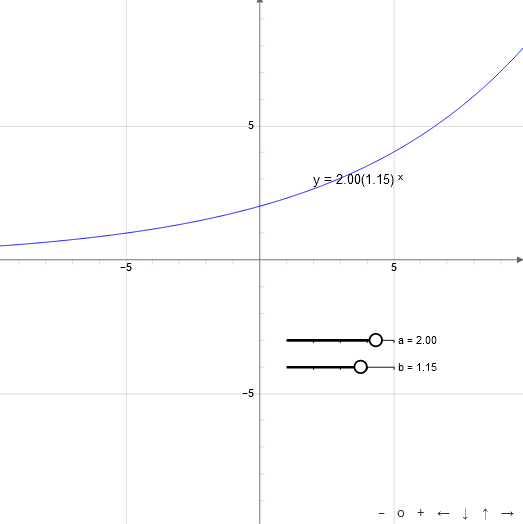
\includegraphics[width=\linewidth]{external/jsxgraph-algebra-general-exponential.png}
\end{sbspanel}%
\begin{sbspanel}{0.21}%

\includegraphics[width=\linewidth]{generated/qrcode/interactive_exponentials-1.png}
\href{http://webwork.bridgew.edu/oer/functions_at_work/interactive_exponentials-1.html}{Standalone}%
\par
\href{http://webwork.bridgew.edu/oer/functions_at_work/interactive_exponentials-1-if.html}{Embed}%
\end{sbspanel}%
\end{sidebyside}%
\tcblower
\end{figureptx}%
In this chapter, we will make extensive use of the \hyperref[exponential-arithmetic]{Properties of Exponential Functions}. If you get stuck duing a computation, it is a good idea to see if there is a property that you may find useful.%
\begin{exploration}{Exploration}{}{ex_exponential-sandard-form}%
Use the laws of exponents to rewrite the following functions in the form \(f(x) = a \cdot b^x\) where \(a,b\) are numbers.%
\begin{enumerate}[font=\bfseries,label=(\alph*),ref=\alph*]%
\item{}Rewrite \(f(x) = 2^{-2x}\) as an exponential function in standard form.%
\par\smallskip%
\noindent\textbf{\blocktitlefont Solution}.\hypertarget{ex_exponential-sandard-form-2-2}{}\quad{}%
\begin{align*}
f(x) \amp = 2^{-2x} \amp \qquad\amp \\
\amp = \dfrac{1}{2^{2x}} \amp \qquad\amp \text{Using } a^{-r} = \frac{1}{a^r} \\
\amp = \dfrac{1}{ (2^2)^{x}} \amp \qquad\amp \text{Using } a^{r\cdot s} = (a^r)^s \\
\amp = \dfrac{1}{ (4)^{x}} \amp \qquad\amp   \\
\amp = \left(\dfrac{1}{ 4}\right)^{x} \amp \qquad\amp \text{Using } \frac{1}{a^{s}} =  \left(\frac{1}{a}\right)^s\\
\amp = {\color{red} 1\cdot} \left(0.25\right)^{x} \amp \qquad\amp 
\end{align*}
Note that in the second to last step, we only had a base and a power.  In the last step, we introduce a coefficient of \(1\), which does not change the value of the expression.%
\par
We have shown that \(f(x)\) is equal to \(a\cdot b^x\) with \(a=1\) and \(b=0.25\).%
\item{}Rewrite \(f(x) = \left(\dfrac{1}{2}\right)^{2x+1}\) as an exponential function in standard form.%
\par\smallskip%
\noindent\textbf{\blocktitlefont Solution}.\hypertarget{ex_exponential-sandard-form-3-2}{}\quad{}%
\begin{align*}
f(x) \amp = \left(\dfrac{1}{2}\right)^{2x+1} \amp \qquad\amp \\
\amp = \left(\dfrac{1}{2}\right)^{2x} \cdot \left(\dfrac{1}{2}\right)^{1} \amp \qquad\amp \text{Using } a^{r+s} =  a^r\cdot a^s\\
\amp = \left(\dfrac{1}{2}\right)^{2x} \cdot \dfrac{1}{2}  \amp \qquad\amp \\
\amp = \left(\left(\dfrac{1}{2}\right)^{2}\right)^x \cdot \dfrac{1}{2} \amp \qquad\amp \text{Using } {\left(a^{r}\right)}^s=  a^{r\cdot s}  \\
\amp = \left(\dfrac{1}{4}\right)^x \cdot \dfrac{1}{2} \amp \qquad\amp \text{Using } \frac{1}{a^{s}} =  \left(\frac{1}{a}\right)^s\\
\amp =  \dfrac{1}{2} \cdot \left(\dfrac{1}{4}\right)^x \cdot \amp 
\end{align*}
We have shown that \(f(x)\) is equal to \(a\cdot b^x\) with \(a=\frac{1}{2}\) and \(b=\frac{1}{4}\).%
\item{}Rewrite \(f(t) = 100 \cdot \left(1 + \dfrac{0.2}{4}\right)^{4t}\) as an exponential function in standard form.%
\par\smallskip%
\noindent\textbf{\blocktitlefont Solution}.\hypertarget{ex_exponential-sandard-form-4-2}{}\quad{}%
\begin{align*}
f(x) \amp =  100 \cdot \left(1 + 0.05\right)^{4t} \qquad\amp \\
f(x) \amp =  100 \cdot \left(1.05\right)^{4t} \qquad\amp \\
f(x) \amp =  100 \cdot \Big(\left(1.05\right)^{4}\Big)^t \qquad\amp \text{Using }{\left(a^{r}\right)}^s=  a^{r\cdot s}\\
f(x) \amp =  100 \cdot \Big(1.2155\Big)^t \qquad\amp 
\end{align*}
We have shown that \(f(t)\) is equal to \(a\cdot b^t\) with \(a=100\) and \(b=1.2155\).%
\end{enumerate}%
\end{exploration}%
\end{sectionptx}
%
%
\typeout{************************************************}
\typeout{Section 5.2 Percents and Percent Change}
\typeout{************************************************}
%
\begin{sectionptx}{Section}{Percents and Percent Change}{}{Percents and Percent Change}{}{}{sec_percent_change}
You should already be familiar with the concept of percents. But because percents play an essential role in many  topics in economics and business, we briefly review the definitions before moving on to our main applications.%
\par
The english word \emph{cent} derives from the Latin word \emph{centum} which means ``hundred''. In other words, \emph{20 percent} literally means \emph{20 per hundred} or \(\dfrac{20}{100} = 0.2\)%
\begin{definition}{Definition}{}{def-percent}%
Given any number \(A\), the expression \emph{\(A\) percent} (also written \(A\)\%) refers to the \emph{decimal rate}%
\begin{equation*}
r = \dfrac{A}{100}
\end{equation*}
%
\par
Given any numbers \(A,P\), you can find \emph{\(A\)\% of \(P\)} by multiplying \(P\) by the decimal rate \(r = \frac{A}{100}\)%
\end{definition}
\begin{example}{Example}{Basic Percentages.}{ex_basic-percentages}%
%
\begin{itemize}[label=\textbullet]
\item{}\(15\)\% is equal to the decimal \(r = \frac{15}{100} = 0.15\)%
\item{}\(2\)\% is equal to the decimal \(r = \frac{2}{100} = 0.02\)%
\item{}\(0.12\)\% is equal to the decimal \(r = \frac{0.12}{100} = 0.0012\)%
\item{}\(15\)\% of \textdollar{}\(40\) is equal to \(40 ( 0.15 )= 6\)%
\item{}\(2\)\% of \textdollar{}\(500\) is equal to \(500 (0.02) = 10\)%
\item{}\(0.12\)\% of \textdollar{}\(30\) is equal to \(30 (0.0012) = 0.036\)%
\end{itemize}
%
\end{example}
\begin{insight}{Application}{Understanding percent change.}{sec_percent_change-6}%
It is common to talk about an economic quanity by changing by a  given percentage.%
\par
The term \terminology{percent} is an abbreviation of the expression \emph{per cent}, which means \emph{per one hundred}. In other words, \(25\)\% is the same thing as \(25\) hundreds, or a decimal rate of \(\dfrac{25}{100}=0.25\).%
\par
For example, \(25\)\% of \(1000\), is equal to \(1000\cdot 0.25 = 250\).%
\par
Now, suppose that you say that \(1000\) \emph{increases} by \(25\) percent.  How much do you have after this increase?%
\par
If you are \emph{increasing} the value by 25\%, you \emph{keep} the original \(1000\), and \emph{add} the new \(250\).  In other words, you have%
\begin{equation*}
1000 + 1000\cdot 0.25 = 1250\text{.}
\end{equation*}
%
\par
Suppose that you increase \(700\) by 25\%.  You take the original \(700\), and add the \(700\cdot 0.25=175\) to get the final value%
\begin{equation*}
700 + 700\cdot 0.25 = 875
\end{equation*}
%
\par
There is a pattern here.  If you take a principal value of \(P\), and increase it by a decimal rate of \(r\), the final value will be%
\begin{equation*}
P + P \cdot r 
\end{equation*}
We can factor a \(P\) out of each term, to get that the result of increasing \(P\) by a decimal rate of \(r\) results in a final value of%
\begin{equation*}
P\cdot (1+r)
\end{equation*}
%
\par
To \emph{decrease} \(1000\) by \(25\)\%, subtract \(0.25 \cdot 1000 = 250\) from \(1000\), resulting in%
\begin{equation*}
1000 - 1000\cdot 0.25 = 1000 - 250 = 750
\end{equation*}
%
\par
To decrease a principal value of \(P\) by a decimal rate of \(r\), compute%
\begin{equation*}
P - P\cdot r = P(1-r)
\end{equation*}
%
\end{insight}
\begin{definition}{Definition}{Percent Change.}{def-percentchange}%
Suppose that \(r\) is a decimal rate, and that \(P\) is any value. \(F\) is the result of \terminology{\emph{increasing} \(P\) by the rate \(r\)} if \(F = P+rP\), also written%
\begin{equation*}
F = P\cdot (1+r)\text{.}
\end{equation*}
%
\par
If \(F\) is the result of \terminology{\emph{decreasing} \(P\) by the rate of \(r\)}, we subtract \(rP\) instead, resulting in the formula%
\begin{equation*}
F = P\cdot (1-r) 
\end{equation*}
%
\end{definition}
\begin{exploration}{Exploration}{}{ex_percentchange1}%
Suppose you begin with \textdollar{}1000.  How much do you have if the value is increased by 25\%, and then decreased by 30\%?%
\par\smallskip%
\noindent\textbf{\blocktitlefont Solution}.\hypertarget{ex_percentchange1-2}{}\quad{}25\% corresponds to a decimal rate of \(r=\frac{25}{100} = 0.25\). To increase \textdollar{}1000 by 25\%, add \textdollar{}1000 to \(1000(0.25)\)%
\begin{equation*}
1000 + 1000(0.25) = 1000 + 250 = 1250
\end{equation*}
We could also just have multiplied \(1000\) by \(1+0.25 = 1.25\)%
\par
30\% corresponds to a decimal rate of \(r = 0.3\).  To decrease \textdollar{}1250 by 30\%, take \textdollar{}1250 and subtract \(1250(0.3)\)%
\begin{equation*}
1250 - 1250(0.3)=875
\end{equation*}
We could also just have multiplied \(1000\) by \(1  + (-0.3) = 0.7\)%
\end{exploration}%
To \emph{find} the percent change between \(F\) and \(P\), set up the equation%
\begin{equation*}
F = P(1+r)
\end{equation*}
and solve for \(r\)%
\begin{exploration}{Exploration}{}{ex_percentchange2}%
\begin{enumerate}[font=\bfseries,label=(\alph*),ref=\alph*]%
\item{}If the balance of your investment goes from \textdollar{}\(300\) to \textdollar{}\(412\), by what percent has it changed?%
\par\smallskip%
\noindent\textbf{\blocktitlefont Solution}.\hypertarget{ex_percentchange2-1-2}{}\quad{}We want to find the percent \(r\) so that%
\begin{equation*}
412 = 300\cdot (1 + r) 
\end{equation*}
Solving for \(r\) gives%
\begin{equation*}
1 + r = \frac{412}{300}  = 1.373333333333333 
\end{equation*}
%
\begin{equation*}
1 + r = 1.373333333333333 
\end{equation*}
%
\begin{equation*}
r = 0.373333333333333
\end{equation*}
The value has increased by 37.33\%%
\item{}If the balance of your investment goes from \textdollar{}\(300\) to \textdollar{}\(234\), by what percent has it changed?%
\par\smallskip%
\noindent\textbf{\blocktitlefont Solution}.\hypertarget{ex_percentchange2-2-2}{}\quad{}We want to find the percent \(r\) so that%
\begin{equation*}
234 = 300\cdot (1 + r) 
\end{equation*}
Solving for \(r\) gives%
\begin{equation*}
1 + r = \frac{234}{300}  = 0.78 
\end{equation*}
%
\begin{equation*}
1 + r = 0.78 
\end{equation*}
%
\begin{equation*}
r = -0.22
\end{equation*}
The value has decreased by 22\%%
\end{enumerate}%
\end{exploration}%
\begin{exploration}{Exploration}{}{ex_percentchange3}%
Let \(P\) be any principal value. For each of the following final values, find out whether the principal has been increased or decreased, and the find the corresponding decimal rate and percent of this change.%
\begin{enumerate}[font=\bfseries,label=(\alph*),ref=\alph*]%
\item{}By what percent has \(P\) been changed, if you end up with a final value of \(1.1 P\)?%
\par\smallskip%
\noindent\textbf{\blocktitlefont Solution}.\hypertarget{ex_percentchange3-2-2}{}\quad{}We want to rewrite \(1.1 P\) in the form \(P(1+r)\) for some number \(r\). Here we have%
\begin{equation*}
1.1P = P(1.1) = P(1 + 0.1)
\end{equation*}
In other words, the principal \(P\) has been increased by a decimal rate of \(0.1\), which corresponds to an increase of \(10 \)\%.%
\item{}By what percent has \(P\) been changed, if you end up with a final value of \(0.85 P\)?%
\par\smallskip%
\noindent\textbf{\blocktitlefont Solution}.\hypertarget{ex_percentchange3-3-2}{}\quad{}We want to rewrite \(0.85 P\) in the form \(P(1+r)\) for some number \(r\). Here we have%
\begin{equation*}
0.85P = P(0.85) = P(1 - 0.15)
\end{equation*}
In other words, the principal \(P\) has been decreased by a decimal rate of \(0.15\), which corresponds to an decrease of \(15 \)\%.%
\item{}By what percent has \(P\) been changed, if you end up with a final value of \(3 P\)?%
\par\smallskip%
\noindent\textbf{\blocktitlefont Solution}.\hypertarget{ex_percentchange3-4-2}{}\quad{}We want to rewrite \(3 P\) in the form \(P(1+r)\) for some number \(r\). Here we have%
\begin{equation*}
3P = P(3) = P(1 +2)
\end{equation*}
In other words, the principal \(P\) has been increased by a decimal rate of \(2\), which corresponds to an increased of \(200 \)\%.%
\end{enumerate}%
\end{exploration}%
We have focused above on understanding and applying the definition of percent change \(F = P(1+r)\), since this will be important to understand compound interest below. However, there are also a variety of other equivalent formulas that can be used to find percent change.%
\begin{corollary}{Corollary}{}{}{cor-percentchange}%
The percent change from \(P\) to \(F\) is given by \(r = \dfrac{F}{P}-1\), or equivalently by \(r = \dfrac{F-P}{P}\)%
\end{corollary}
\begin{proof}{Proof}{}{cor-percentchange-2}
To get both equations, solve \(F = P(1+r)\) for \(r\). For the first,%
\begin{align*}
F \amp = P(1+r) \\
\dfrac{F}{P} \amp = 1 + r\\
\dfrac{F}{P} - 1 \amp = r
\end{align*}
For the second,%
\begin{align*}
F \amp = P(1+r) \\
F \amp = P+ Pr \\
F - P \amp = Pr \\
\dfrac{F - P}{P} \amp = r \qedhere
\end{align*}
%
\end{proof}
\end{sectionptx}
%
%
\typeout{************************************************}
\typeout{Section 5.3 Compound Interest and Depreciation}
\typeout{************************************************}
%
\begin{sectionptx}{Section}{Compound Interest and Depreciation}{}{Compound Interest and Depreciation}{}{}{sec_compound_interest}
The power mathematics comes from the fact that the same basic tools apply in a surprisingly wide variety of contexts. For example, percent changes occur in many contexts including%
\begin{itemize}[label=\textbullet]
\item{}loan payments,%
\item{}inflation, and%
\item{}the change in value of physical objects.%
\end{itemize}
In finance, your hope is that the value of your investments will increase over time. In other contexts (manufacturing, purchasing a car, etc.), you understand that the value of your investment will \emph{decrease} over time. The process of an object losing value over time is called \terminology{depreciation}.%
\par
To describe the results of inflation at a fixed percent (say, 4\%) over several years, or to describe an object that repeatedly decreases in value by a fixed percent over several years, we will need a formula for repeated percent changes.%
\begin{insight}{Application}{Repeated percent changes.}{sec_compound_interest-4}%
Inflation refers to the process of prices increasing over time. Often, we talk about prices increasing at the same rate per year, over a period of several years.%
\par
For example, suppose that prices are increasing at \(5\)\% per year, which corresponds to a decimal rate \(r = \frac{5}{100}=0.05\). Suppose also that a certain product costs \(100\)\textdollar{} in the first year.%
\par
One year later, the cost is the original amount \(P=100\) plus a change of \(rP = 0.05\cdot 100 = 5\) dollars.  In other words, the value one year later is%
\begin{equation*}
V(1) = 100 + 0.05\cdot 100 = 105.
\end{equation*}
In our notation for percent change, we can also write this as%
\begin{equation*}
V(1) = 100 \cdot (1+0.05) = 105.
\end{equation*}
%
\par
How much will the value be after two years? In the second year, the value of \(105\) increases a second time, also by 5\%, or a rate of \(r=0.05\).  That means%
\begin{equation*}
V(2) = 105 + 105\cdot 0.05 = 110.25
\end{equation*}
In our notation for percent change, we can write this as%
\begin{equation*}
V(2) = 105\cdot (1+0.05) = 105\cdot (1.05)
\end{equation*}
But the leading coefficent of \(105\) can also be rewritten, since \(105 = 100\cdot (1.05)\).  In other words,%
\begin{equation*}
V(2) = 100 \cdot (1.05) \cdot (1.05) = 100\cdot (1.05)^2
\end{equation*}
%
\par
We can find the value after three years in the same way. We will take the value from the second year, and increase it by a rate of \(r=0.05\). Furthermore, that increase is equivalent to multiplying the value from the second year by another coefficient of \(1+0.05=1.05\).%
\begin{equation*}
V(3) = 100 \cdot (1.05)\cdot (1.05)\cdot (1.05) = 100\cdot (1.05)^3
\end{equation*}
%
\par
This line of reasoning works for any positive period of time \(t\), giving us a formula for the value of an object with original value \(100\), where the price has been increased 5\% for \(t\) years.%
\begin{equation*}
V(t) = 100 \cdot (1.05)^t = 100\cdot (1 + 0.05)^t
\end{equation*}
%
\end{insight}
\begin{proposition}{Proposition}{}{}{prop-compounding}%
Suppose that an original principal value of \(P\) is repeatedly changed by a fixed decimal rate of \(r\) \alert{one time per year}.  The value after \(t\) years will be given by%
\begin{equation*}
V(t) = P \cdot \Big( 1 + r \Big)^t\text{.}
\end{equation*}
%
\par
If the value is being increased, use a posive value for the rate \(r\).  If the value is being decreased, use a negative value for the rate \(r\).%
\end{proposition}
Accountants often keep track of the present value of a larged investment or fixed asset. The term \terminology{depreciation} refers to a decrease in the value of the asset. You can find a more complete introduction to the concept on Investopedia at \href{https://www.investopedia.com/terms/d/depreciation.asp}{\nolinkurl{https://www.investopedia.com/terms/d/depreciation.asp}}.%
\begin{insight}{Application}{Accounting and depreciation.}{insight-depreciation}%
Value can be measured in many ways. For example, suppose that you purchase a car and that you somehow know that it will last 200,000 miles, and that you will drive 20,000 miles each year. By how much has the value value of the car decreased after 3 years?%
\par
The "correct" answer to this question depends on a surprising number of factors.%
\begin{itemize}[label=\textbullet]
\item{}If you are measuring value as "percent of lifetime miles remaining", there would be \(160,000\) of the total \(200,000\) miles remaining, so the value of the car would be \(\frac{160,000}{200,000} = 0.8\), or 80\%, of its original value.%
\par
After four years, the value of the car would be  \(\frac{140,000}{200,000} = 0.7\), or 70\%, of its original value. And after five years, the value of the car would be  \(\frac{120,000}{200,000} = 0.6\), or 60\%, of its original value.%
\par
In this case, the value is decreasing at a constant amount per year.  This is often called \terminology{straight line depreciation}, since connecting the dots yields a linear equation%
\begin{equation*}
\text{(value at year t)} = \text{(starting value)} - \text{(amount of value used per year)} t
\end{equation*}
%
\item{}On the other hand, cars are known to break more and more frequently as they get older.  If you knew which repairs would be required each year, you could make a table of values telling you the value of the vechicle at each point in time (or at each number of miles).  For each year, you would take its value from the previous year, decrease the value based on the reduced mileage of the car, and subtract the expected maintenence from that point of time.%
\par
This way of tracking the decrease, or depreciation, is in some ways more accurate than straightline depreciation but is much more complicated to compute.%
\item{}From a different perspective, it is clear that new cars have many features that older cars do not.  To oversimplify things, suppose  that a new car always has 10\% more features than an older car.  If you are going to buy a car that is one year older, you will want the price to decrease enough to make up for that loss in additional features.%
\par
Said another way, many investments will lose a fixed percent of their value every year.  This is called \terminology{declining balance} depreciation.%
\par
Suppose that the value of a different car decreases by 25\% each year.  After one year, 75\% of the value is retained.  After 2 years, 75\% of the original 75\% is retained, resulting in \(0.75\cdot 0.75= 0.5625\), or 56.25\% of the value remains.  After 3 years, the value that remains is  \(0.75\cdot 0.75\cdot 0.75= 0.421875\), or 42.19\% of the original value.%
\par
More generally, the value after \(t\) years is defined by the exponential equation%
\begin{equation*}
\text{(value in year t)} = \text{(starting value)}\cdot \text{(percent of value retained after a year)}^t
\end{equation*}
%
\end{itemize}
%
\par
Deciding when to use each depreciation scheme is an important question in Accounting, and is well beyond the scope of this course. As a result, in this course, we will restrict our attention to declining balance depreciation, and we will usually state explicitly that a fixed percentage of value is lost each year.%
\end{insight}
\begin{exploration}{Exploration}{}{ex_depreciation1}%
Your company has recently invested in a \textdollar{}500,000 CNC machine for a high throughput production line. After some research, you have decided that each year, the machine will lose 20\% of its remaining value.%
\begin{enumerate}[font=\bfseries,label=(\alph*),ref=\alph*]%
\item{}What is the net value of the asset after one year?  After two years?%
\par\smallskip%
\noindent\textbf{\blocktitlefont Solution}.\hypertarget{ex_depreciation1-2-2}{}\quad{}After one year, the value is%
\begin{align*}
V(1) \amp = 500,000 - 0.2\cdot 500,000\\
\amp = 500,000 - 100,000\\
\amp = 400,000 
\end{align*}
After two years, the value is%
\begin{align*}
V(2) \amp = 400,000 - 0.2\cdot 400,000\\
\amp = 400,000 - 80,000\\
\amp = 320,000 
\end{align*}
%
\item{}Find a formula for the future value of the asset as a function of the number of years \(t\) in the future. Sketch a graph of this function.%
\par\smallskip%
\noindent\textbf{\blocktitlefont Solution}.\hypertarget{ex_depreciation1-3-2}{}\quad{}We are repeatedly reducing the principal (original value) \(P=500,000\) by 20\%, or a decimal rate of \(r= -0.2\). Using \hyperref[prop-compounding]{Proposition~{\xreffont\ref{prop-compounding}}}, we see that the value of the investment at time \(t\) is given by%
\begin{align*}
V(t) = \amp  P\cdot (1 + r)^t \\
= \amp 500,000\cdot (1 + (-0.2))^t \\
= \amp 500,000\cdot (0.8)^t 
\end{align*}
%
\par
In other words, 80\% of the value is retained each year.  We can now use this formula to answer the first part of the question:%
\begin{equation*}
V(1) = 500,000 \cdot ( 1 - 0.2 )^1 = 500,000 \cdot 0.8 = 400,000
\end{equation*}
%
\begin{equation*}
V(2) = 500,000 \cdot ( 1 - 0.2 )^2 = 500,000 \cdot (0.8)^2 = 320,000
\end{equation*}
%
\begin{image}{0.25}{0.5}{0.25}{}%
\resizebox{\linewidth}{!}{%
\begin{tikzpicture}
    [scale=0.5,
    declare function = {
    f(\x) = 5*(0.8)^(\x);
    xmin=-2.5;
    xmax=5.5;
    ymin=-0.5;
    ymax=7.5;
    pad=1;
    domainstart=-1;
    domainstop=4.5;
    }]
  \draw[axes] (0,ymin-pad)--(0,ymax+pad);
  \draw[axes] (xmin-pad,0)--(xmax+pad,0);

  % Graph the function defined in the TikZ environment
  \draw [color=blue,curve,domain=domainstart:domainstop,smooth] plot ({\x},{f(\x)});
  
  \draw[color=red,fill] (0,{f(0)}) circle (3pt);
  \draw[color=red,fill] (1,{f(1)}) circle (3pt);
  \draw[color=red,fill] (2,{f(2)}) circle (3pt);
  \draw[color=red,fill] (3,{f(3)}) circle (3pt);
  \draw[color=red,fill] (4,{f(4)}) circle (3pt);

\end{tikzpicture}
}%
\end{image}%
\end{enumerate}%
\end{exploration}%
\begin{insight}{Application}{Compound interest.}{sec_compound_interest-9}%
The process of repeatedly increasing a value by a fixed percent is called \terminology{compounding}. If you increase the value every year, you are said to be compounding yearly. If you increase the value 12 times per year, you are said to be compounding monthly.%
\par
The term \terminology{interest} refers to a very specfic kind of compounding.  As Investopedia puts it, ``Interest is the monetary charge for borrowing money—generally expressed as a percentage, such as an annual percentage rate (APR).'' (\href{https://www.investopedia.com/terms/i/interest.asp}{\nolinkurl{https://www.investopedia.com/terms/i/interest.asp}})%
\par
In \terminology{compound interest}, you pay interest on both the principal and on the interest accrued so far.%
\par
The term \terminology{compounding} refers to the action of computing the new interest, and adding it back into the principal.%
\par
The simplest example (which we have already mentioned above) happens when the For example, suppose that you borrow \textdollar{}100, at an interest rate of 3\%, and that the interest is compounded (or added to the principal value) \(one time\) each year.%
\begin{tableptx}{Table}{\textbf{Interest Compounded Yearly}}{sec_compound_interest-9-7}{}%
\centering%
{\tabularfont%
\begin{tabular}{lAlAlAl}
Years Elapsed&Previous Debt&New interest&New Debt\tabularnewline\hrulethin
\(1\)&\(100\)&\(100\cdot 0.03=3\)&\(100+3=103\)\tabularnewline\hrulethin
\(2\)&\(100\)&\(100\cdot 0.03=3.09\)&\(103+3.09=106.09\)
\end{tabular}
}%
\end{tableptx}%
Often, interest will be compounded multiple times each year.  Suppose, for example, that you borrow money at 3\% interest, compounded \emph{twice} each year.%
\par
Does this mean that you need to pay 3\% interest after 6 months, and a \emph{second} 3\% interest after the next 6 months? Absolutely not - that would be like paying 6\% interest over the year!%
\par
Instead, the convention is to divide the state \terminology{annual percentage rate} evenly among the number of compoundings per year.  For example, if you borrow at 3\% compounded twice per year, then the \emph{interest per compounding} is \(\frac{3 \%}{2\text{ compoundings}} = 1.5\) \% per compounding, or a decimal rate of 0.015 per compounding.%
\begin{tableptx}{Table}{\textbf{Interest Compounded Biannualy}}{sec_compound_interest-9-11}{}%
\centering%
{\tabularfont%
\begin{tabular}{lAlAlAl}
Years Elapsed&Previous Debt&New interest&New Debt\tabularnewline\hrulethin
\(0.5\)&\(100\)&\(100\cdot 0.015=1.5\)&\(100+1.5 = 101.5\)\tabularnewline\hrulethin
\(1.0\)&\(101.5\)&\(101.5\cdot 0.015=1.5225\)&\(101.5+1.5225=103.0225\)\tabularnewline\hrulethin
\(1.5\)&\(103.0225\)&\(103.0225\cdot 0.015=1.5453375 \)&\(103.0225+1.5453375=104.5678375\)\tabularnewline\hrulethin
\(2.0\)&\(104.5678375\)&\(104.5678375\cdot 0.015=1.5685175625\)&\(104.5678375+1.5685175625= 106.136355062 \)
\end{tabular}
}%
\end{tableptx}%
Most banking instruments are compounded monthly, or more frequently. That means that you would compound \(m=12\) times each year, with an interest per compounding of \(\dfrac{3\%}{12\text{ compoundings}}=0.25\) \% per compounding, or a decimal rate of \(r = 0.0025\).%
\par
We could compute this using a table, but you can see that this rapidly becomes unworkable.  Instead, we can modfiy the for repeatedly changing the principal by a fixed value.%
\end{insight}
\begin{definition}{Definition}{}{def-compoundinterest}%
Suppose that a principal \(P\) is invested at an annual decimal rate \(r\), and compounded \(m\) times each year.  The value of the investment after \(t\) years is equal to%
\begin{equation*}
F(t) = P \cdot \left(1 + \frac{r}{m}\right)^{m\cdot t}
\end{equation*}
%
\par
The rate \(r\) is called the \terminology{annual percentage rate}, and the value at year \(t\) is called the \terminology{future value} of the investment at time \(t\).%
\par
The \emph{interest earned} is the difference between the principle and the future value.%
\end{definition}
To remember the formula, remember that you are increasing the principal by the decimal rate \(\frac{r}{m}\) each compounding.  Because you are computing \(m\) times per year, after \(t\) years, you will have repeated this process \(m\cdot t\) times.%
\begin{exploration}{Exploration}{}{ex_compoundinterest1}%
Suppose that you have invested \textdollar{}1000 at an APR of 3\%, compounded monthly.%
\begin{enumerate}[font=\bfseries,label=(\alph*),ref=\alph*]%
\item{}Find the future value of this instrument as a function of the number years \(t\).%
\par\smallskip%
\noindent\textbf{\blocktitlefont Solution}.\hypertarget{ex_compoundinterest1-2-2}{}\quad{}Use the compound interest formula with \(P=1000\), \(r=0.03\), \(m=12\), and time represented by the variable \(t\).%
\begin{equation*}
F(t) = 1000\cdot \left( 1 + \frac{0.03}{12}\right)^{12 t}
\end{equation*}
%
\item{}Find the future value after 10 years and six months.%
\par\smallskip%
\noindent\textbf{\blocktitlefont Solution}.\hypertarget{ex_compoundinterest1-3-2}{}\quad{}10 years and 6 months corresponds to 10.5 years.  Using the compound interest formula,%
\begin{equation*}
F(10.5) = 1000\cdot \left( 1 + \frac{0.03}{12}\right)^{12 (10.5)} = 136.972077476
\end{equation*}
The future value after 10.5 years is approximately \textdollar{}\(1369.72\)%
\item{}Rewrite the future value function in the form \(a\cdot b^t\) where \(a,b\) are numbers.%
\par\smallskip%
\noindent\textbf{\blocktitlefont Solution}.\hypertarget{ex_compoundinterest1-4-2}{}\quad{}In the expression%
\begin{equation*}
F(t) = 1000\cdot \left( 1 + \frac{0.03}{12}\right)^{12 t}
\end{equation*}
the base \(1 + \frac{0.03}{12} = 1.0025 \) is a single number.  That lets us rewrite the expression as%
\begin{equation*}
F(t) = 1000\cdot \left( 1.0025 \right)^{12 t}
\end{equation*}
Next, we can use the property of exponents \(a^{r\cdot s} = {\left(a^{r}\right)}^s\) to rewrite the expression as%
\begin{equation*}
F(t) = 1000\cdot \left( 1.0025^{12} \right)^{t}
\end{equation*}
Now we can again simplify the base \(1.0025^{12} = 1.03041595691\), which gives the expression%
\begin{equation*}
F(t) = 1000\cdot \left( 1.03041595691 \right)^{t}
\end{equation*}
We have now written \(F(t) = a \cdot b^t\) with \(a=1000\) and \(b = 1.03041595691\).%
\item{}What is the \terminology{effective} annual interest rate?  In other words, what is the  \emph{actual} percentage by which the balance increases every year?%
\par\smallskip%
\noindent\textbf{\blocktitlefont Solution}.\hypertarget{ex_compoundinterest1-5-2}{}\quad{}Recall that \(P\cdot (1+ r)^t\) gives the result of increasing the value \(P\) by a rate of\(r\), repeated \(t\) times.%
\par
We have shown above that the future value is given by%
\begin{equation*}
F(t) = 1000\cdot \left( 1.03041595691 \right)^{t}
\end{equation*}
Rewriting this we get%
\begin{equation*}
F(t) = 1000\cdot \left( 1 + 0.03041595691 \right)^{t}
\end{equation*}
In other words, this is equivalent to increasing the value by an \emph{actual}, or \emph{effective}, rate of \(3.041\dots\) percent each year.%
\end{enumerate}%
\end{exploration}%
\begin{definition}{Definition}{}{def-effectiveapr}%
The \terminology{effective APR} of an investment is the rate \(r_{eff}\) such that%
\begin{equation*}
P \cdot \Big(1 + \frac{r}{m}\Big)^{m\cdot t} = P \cdot \Big(1 + r_{eff}\Big)^{t}
\end{equation*}
%
\end{definition}
\begin{insight}{Application}{Another way to find Effective APR.}{sec_compound_interest-14}%
Given the definition of effective APR, it is generally easist to find the effective APR by using the laws of exponents to simplify the compound interest formula with your given values.%
\par
This approach may, however, make it a bit more difficult to see the actual meaning of \(r_{eff}\). To make this meaning more clear, we will introduce another more numerical way to compute \(r_{eff}\).%
\par
Recall that the \emph{effective APR} of an investment tells you the \emph{actual} percent by which the value grows each year. That means that you can also find the effective APR by \emph{computing and comparing the value of the investment at any conscutive two years}.%
\par
For example, in the the exercise above, we found that the future value was given by%
\begin{equation*}
F(t) = 1000\cdot \left( 1 + \frac{0.03}{12}\right)^{12 t}\text{.}
\end{equation*}
That means that the value in year \(0\) is%
\begin{equation*}
F(0) = 1000\cdot \left( 1 + \frac{0.03}{12}\right)^{12 (0) = 1000}
\end{equation*}
and that the value in year \(1\) is%
\begin{equation*}
F(1) = 1000\cdot \left( 1 + \frac{0.03}{12}\right)^{12 (1)} = 1030.41595691\text{.}
\end{equation*}
To find the percent change from years 0 to 1, we can compute the ratio%
\begin{equation*}
\dfrac{F(1)}{F(0)} = \dfrac{1030.41595691}{1000} = 1.03041595691
\end{equation*}
Between years 0 and 1, the principal has been increased by a multiple of%
\begin{equation*}
1.03041595691 = 1 + 0.03041595691
\end{equation*}
which corresponds to a decimal rate of  \(r_{eff}=  0.03041595691\), or a percent rate of 3.041595691\%%
\end{insight}
\begin{exploration}{Exploration}{}{ex_compoundinterest2}%
You invest in a company at 20\%, compounded quarterly.%
\begin{enumerate}[font=\bfseries,label=(\alph*),ref=\alph*]%
\item{}If you start with \textdollar{}100, find the balance as a function of time \(t\) in years.  What is the balance after 1 year?%
\par\smallskip%
\noindent\textbf{\blocktitlefont Solution}.\hypertarget{ex_compoundinterest2-2-2}{}\quad{}Start by writing down the formula for  \hyperref[def-compoundinterest]{Definition~{\xreffont\ref{def-compoundinterest}}}.%
\begin{equation*}
F(t) = P \cdot \left(1 + \frac{r}{m}\right)^{m\cdot t}
\end{equation*}
Using the principal \(P=100\), decimal rate \(r=0.2\), and frequency of compounding \(m=4\), since there are four quarters in each year.%
\par
That gives the equation%
\begin{equation*}
F(t) = 100 \cdot \left(1 + \frac{0.2}{4}\right)^{4\cdot t}
\end{equation*}
We could stop there, but it is often nice to clean this up by  simplifying the base of the exponent to get a formula for the value after \(t\) years%
\begin{equation*}
F(t) = 100 \cdot \left(1.05 \right)^{4\cdot t}
\end{equation*}
%
\par
To find the value after one year, plug in \(t=1\) and simplify,%
\begin{equation*}
F(1) = 100 \cdot \left(1.05 \right)^{4\cdot 1} = \dots = 100\cdot 1.2155 = 121.55
\end{equation*}
%
\item{}How much should you start with to get \textdollar{}1000 after 5 years?%
\par\smallskip%
\noindent\textbf{\blocktitlefont Solution}.\hypertarget{ex_compoundinterest2-3-2}{}\quad{}Again, start by writing down the formula for  \hyperref[def-compoundinterest]{Definition~{\xreffont\ref{def-compoundinterest}}}%
\begin{equation*}
F(t) = P \cdot \left(1 + \frac{r}{m}\right)^{m\cdot t}\text{.}
\end{equation*}
Next, fill in the values given.  In this problem, we want the \emph{future value} \(F=1000\) at the \emph{future time} \(t=5\). We are also given \(r=0.2\) and \(m=4\).%
\begin{equation*}
1000 = P \cdot \left(1 + \frac{0.2}{4}\right)^{4\cdot 5}\text{.}
\end{equation*}
Note that now the unknown variable is the starting (or present) value \(P\).%
\par
Simplifying the base and exponents gives%
\begin{equation*}
1000 = P \cdot \left(1.05\right)^{20}
\end{equation*}
Using a calculator, we obtain%
\begin{equation*}
1000 = P \cdot 2.6532
\end{equation*}
Solve for \(P\) by dividing both sides by \(2.6532\)%
\begin{equation*}
P = \dfrac{1000}{2.632} = 376.89
\end{equation*}
You must start with a present value \(P=376.89\) to achieve the desired future value in 5 years.%
\item{}Rewrite \(F(t)\) in the form \(a\cdot b^t\).  What is the effective APR?%
\par\smallskip%
\noindent\textbf{\blocktitlefont Solution}.\hypertarget{ex_compoundinterest2-4-2}{}\quad{}Again, start by writing down the formula for  \hyperref[def-compoundinterest]{Definition~{\xreffont\ref{def-compoundinterest}}}%
\begin{equation*}
F(t) = P \cdot \left(1 + \frac{r}{m}\right)^{m\cdot t}\text{.}
\end{equation*}
Next, fill in the values given.%
\begin{equation*}
F(t) = P \cdot \left(1 + \frac{0.2}{4}\right)^{4\cdot t}\text{.}
\end{equation*}
No other values are given in this part, so we now simplify.%
\begin{equation*}
F(t) = P \cdot \left(1.05\right)^{4\cdot t}
\end{equation*}
Using the law of algebra \(a^{rs} = (a^r)^s\), we get%
\begin{align*}
F(t) = \amp P \cdot \left(1.05^4\right)^{t}\\
= \amp P \cdot \left(1.2155\dots \right)^{t} \\
= \amp P \cdot \left(1 + 0.2155\dots \right)^{t} 
\end{align*}
Recall \hyperref[prop-compounding]{Proposition~{\xreffont\ref{prop-compounding}}}.  This reminds us that the expression above coressponds to the process of repeatedly increasing the principal \(P\) by \(21.55\dots\)\% each year.%
\par
In other words, the effective APR is \(21.55\dots\)\%.%
\end{enumerate}%
\end{exploration}%
\begin{inlineexercise}{Checkpoint}{}{ex_compoundinterest3}%
How much must you invest at 3\% interest, compounded monthly, to have 10,000 after 5 years?%
\par\smallskip%
\noindent\textbf{\blocktitlefont Solution}.\hypertarget{ex_compoundinterest3-2}{}\quad{}Again, start by writing down the formula for  \hyperref[def-compoundinterest]{Definition~{\xreffont\ref{def-compoundinterest}}}%
\begin{equation*}
F(t) = P \cdot \left(1 + \frac{r}{m}\right)^{m\cdot t}\text{.}
\end{equation*}
Next, fill in the values given.%
\begin{equation*}
10000 = P \cdot \left(1 + \frac{0.03}{12}\right)^{12\cdot 5}\text{.}
\end{equation*}
We want to solve for the unknown variable \(P\).  We could simplify the expression using a calculator, or we could just use the fact that \(\left(1 + \frac{0.03}{12}\right)^{12\cdot 5}\) is a constant number and divide both sides by it to get.%
\begin{equation*}
P = \dfrac{10,000}{\left(1 + \frac{0.03}{12}\right)^{12\cdot 5}} = 8,609\text{.}
\end{equation*}
%
\par
%
\end{inlineexercise}%
\emph{A picture is worth a thousand words}. The present value will grow more fast or slow based on the value of the principal \(P\), APR \(r\), and frequency of compounding \(m\).  In the graphic below, use the sliders to change these two numbers, and get a sense of how fast each of these parameters impact the growth of a balance compounded continuously.%
\begin{figureptx}{Figure}{Compound interest as a function of time}{sec_compound_interest-18}{}%
\begin{sidebyside}{2}{0.075}{0.075}{0.17}%
\begin{sbspanel}{0.47}%
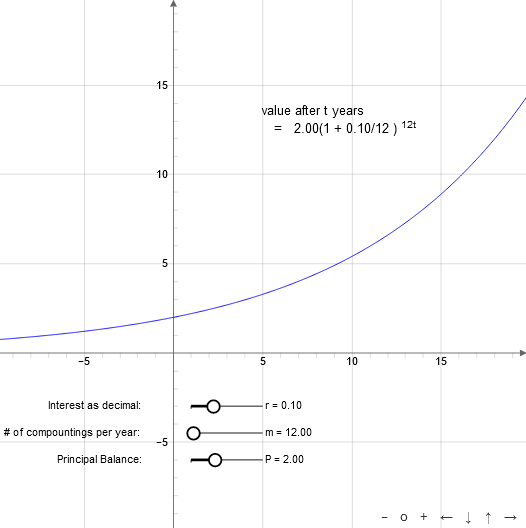
\includegraphics[width=\linewidth]{external/jsxgraph-algebra-compound-interest.png}
\end{sbspanel}%
\begin{sbspanel}{0.21}%

\includegraphics[width=\linewidth]{generated/qrcode/sec_compound_interest-18-2.png}
\href{http://webwork.bridgew.edu/oer/functions_at_work/sec_compound_interest-18-2.html}{Standalone}%
\par
\href{http://webwork.bridgew.edu/oer/functions_at_work/sec_compound_interest-18-2-if.html}{Embed}%
\end{sbspanel}%
\end{sidebyside}%
\tcblower
\end{figureptx}%
\begin{paragraphs}{The Natural Exponential for Calculus.}{subsec-naturalexp}%
\begin{insight}{Application}{Compounding Faster and Faster.}{subsec-naturalexp-2}%
In the interactive graphic above, note that once you increase the frequency \(m\) above about 20, the graph of compound interest appears to stop changing.%
\par
Actually, if you compute things out with a calculator, you will see that there \emph{are} differences when you change \(m\), but those changes get smaller and smaller as you increase \(m\).%
\par
Fix an APR of \(r=1\) (a rate  of 100\%).%
\begin{center}%
{\tabularfont%
\begin{tabular}{lBlBl}
Frequency of compounding \(m\)&Future Value function \(F(t)\)&Effective APR \(r_{eff}\)\tabularnewline\hrulemedium
1&\(F = P\cdot(1+\frac{1}{1})^{1t} = P\cdot (2)^t\)&\(r_{eff} = 2- 1 = 1\)\tabularnewline\hrulemedium
10&\(F = P\cdot(1+\frac{1}{10})^{10t} = P\cdot (2.59\dots)^t\)&\(r_{eff} \approx 2.59-1 = 1.59\)\tabularnewline\hrulemedium
20&\(F = P\cdot(1+\frac{1}{20})^{20t} = P\cdot (2.59\dots)^t\)&\(r_{eff}\approx 2.65-1 = 1.65\)\tabularnewline\hrulemedium
100&\(F = P\cdot(1+\frac{1}{100})^{100t} = P\cdot (2.70\dots)^t\)&\(r_{eff}\approx 2.70-1 = 1.70\)\tabularnewline\hrulemedium
1000&\(F = P\cdot(1+\frac{1}{1000})^{1000t} = P\cdot (2.71\dots)^t\)&\(r_{eff}\approx 2.71-1=1.71\dots\)\tabularnewline\hrulemedium
\end{tabular}
}%
\end{center}%
In other words, as you compound more and more frequently at an APR of 100\%, the \emph{effective} APR settles down to a specific number (171\%).%
\par
Said another way, as you compound more and more frequently at 100\%, the base settles down on a specific number \(2.71\dots\). Mathematicians use the letter \(e\) to denote this number.%
\end{insight}
Surprisingly, there is a very simple equation for what happens when you compound continuously.%
\begin{theorem}{Theorem}{}{}{thm-continuouscompounding}%
If you compound \terminology{continuously} at a rate \(r\), the value after \(t\) years is given by the function%
\begin{equation*}
F(t) = P\cdot \Big(e^r\Big)^t
\end{equation*}
where \(e\) is a number that is approximately \(2.71\dots\).%
\end{theorem}
Surprisingly, exponential functions with base \(e\) play a very important role in calculus.  Because of this, we call it the \emph{natural} base to use for the exponential function.  More precisely, we make the following definition.%
\begin{definition}{Definition}{}{def-naturalexp}%
The function \(y = e^{x}\) is called the \terminology{natural exponential function}.  Sometimes, we denote this function by writing%
\begin{equation*}
exp(x) = e^x
\end{equation*}
%
\end{definition}
\end{paragraphs}%
\end{sectionptx}
\end{chapterptx}
 %
%
\typeout{************************************************}
\typeout{Chapter 6 Logarithms and Solving for Time}
\typeout{************************************************}
%
\begin{chapterptx}{Chapter}{Logarithms and Solving for Time}{}{Logarithms and Solving for Time}{}{}{ch_logarithms}
\renewcommand*{\chaptername}{Chapter}
\begin{introduction}{}%
In the previous section, we used exponential functions to compute the value of compound interest as a function of time.  For example, Investing \textdollar{}100 and 25\% interest compounded yearly follows the function%
\begin{equation*}
F = 100\cdot (1.25)^t
\end{equation*}
%
\par
Often, you will be given the principal, rate, and frequency of compounding, and you will need to \emph{find the amount of time} you will have to wait to achieve a certain future balance.  If, in the example above, you want to find the time needed to achieve a balance of \textdollar{}4000, you will need to solve the equation%
\begin{equation*}
4000 = 100\cdot (1.25)^t\text{.}
\end{equation*}
This is equivalent to%
\begin{equation*}
40 = \cdot (1.25)^t\text{,}
\end{equation*}
but now we are stuck, since the \(t\) is trapped inside the exponent.%
\par
To get further, we will need to "undo" our compound interest calculation. Mathematically, this means that we will need an \emph{inverse} function.%
\end{introduction}%
%
%
\typeout{************************************************}
\typeout{Section 6.1 Inverse Functions}
\typeout{************************************************}
%
\begin{sectionptx}{Section}{Inverse Functions}{}{Inverse Functions}{}{}{sec-inverses}
Recall that a \terminology{one-to-one} function sends each input to a \emph{different} output.%
\begin{example}{Example}{Exploring the definition of one-to-one.}{eg_onetoone}%
This definition is easiest to apply when you are thinking about functions defined using arrow diagrams.%
\begin{image}{0}{1}{0}{}%
\resizebox{\linewidth}{!}{%
\begin{tikzpicture}
    \draw (0,0) ellipse [x radius=1cm,y radius=2cm];
    \draw (3,0) ellipse [x radius=1cm,y radius=2cm];
    \node(1) at (0,1) {$1$};
    \node(2) at (0,0) {$2$};
    \node(3) at (0,-1) {$3$};
    \node(a) at (3,1) {$a$};
    \node(b) at (3,0) {$b$};
    \node(c) at (3,-1) {$c$};
    \draw[-latex,very thick,red] (1)--(a) node [midway,above] {$f$};
    \draw[-latex,very thick,blue] (2)--(c);
    \draw[-latex,very thick,green] (3)--(b);
    \node at (1,-3) {The function $f$ \emph{is} 1-1};
\end{tikzpicture}
\qquad
\begin{tikzpicture}
    \draw (0,0) ellipse [x radius=1cm,y radius=2cm];
    \draw (3,0) ellipse [x radius=1cm,y radius=2cm];
    \node(1) at (0,1) {$1$};
    \node(2) at (0,0) {$2$};
    \node(3) at (0,-1) {$3$};
    \node(a) at (3,1) {$a$};
    \node(b) at (3,0) {$b$};
    \node(c) at (3,-1) {$c$};
    \draw[-latex,very thick,red] (1)--(a) node [midway,above] {$g$};
    \draw[-latex,very thick,blue] (2)--(b);
    \draw[-latex,very thick,green] (3)--(b);
    \node at (1,-3) {The function $g$ is \emph{not} 1-1};
\end{tikzpicture}
}%
\end{image}%
\end{example}
If your function is one-to-one, then flipping the arrows gives you a \emph{new} function that \emph{undoes} your original function. That new function is called the \terminology{inverse} of the original function.%
\begin{definition}{Definition}{}{def-inverse}%
Let \(f\) be a one-to-one function. Its \terminology{inverse} is the function, written \(f^{-1}\), which satisfies%
\begin{gather*}
f(x)   =    y \\
\iff      \\
x     =    f^{-1}(y) 
\end{gather*}
%
\end{definition}
In \hyperref[eg_onetoone]{Example~{\xreffont\ref{eg_onetoone}}}, the function \(f\) has an inverse function \(f^{-1}\), defined by flipping each of the arrows. For example, because \(f(2) = c\), we have \(f^{-1}(c) = 2\).%
\par
\alert{Danger Zone:} In general, the inverse \(f^{-1}\) is \alert{not} the same thing as the reciprocal.  In other words, \(f^{-1}(x)\) is \alert{not} \(\dfrac{1}{f(x)}\) in general.%
\begin{assemblage}{Summary}{Key Idea.}{assemblage-inverses}%
Inverse functions swich the roles of \(x\) and \(y\) (of input and ouput).%
\end{assemblage}
\begin{example}{Example}{Understanding Inverses Graphically.}{sec-inverses-9}%
Graphically, reversing the roles of input and ouput is the same thing as reflecting the graph of the function across the diagonal line \(y=x\).%
\begin{image}{0}{1}{0}{}%
\resizebox{\linewidth}{!}{%
        \begin{tikzpicture}
          \draw[axes] (0,2) -- (0,-2);
          \draw[axes] (2,0) -- (-2,0);
          \draw [domain=-1.259:1.259,curve] plot ({\x}, {(\x)^3}) node[above] {$y = f(x)$};
          \draw [dashed] (-1.75,-1.75) -- (1.75,1.75) node [right] {$y=x$};

%          \begin{scope}[shift={(5,0)}]
%            \draw (0,2) -- (0,-2);
%            \draw (2,0) -- (-2,0);	
%            \draw [domain=0:2,curve] plot ({\x}, {(\x)^(0.333)}) node [below right] {$y = f^{-1}(x)$};
%            \draw [domain=0:2,curve] plot ({-\x}, {-(\x)^(0.333)});
%            \draw [dashed] (-1.75,-1.75) -- (1.75,1.75) node [right] {$y=x$};
%          \end{scope}
          
          \begin{scope}[shift={(5,0)}]
            \draw[axes] (0,2) -- (0,-2);
            \draw[axes] (2,0) -- (-2,0);	
            \draw [domain=-1.259:1.259,curve] plot ({(\x)^3},{\x}) node [below right] {$y = f^{-1}(x)$};
            \draw [dashed] (-1.75,-1.75) -- (1.75,1.75) node [right] {$y=x$};
          \end{scope}
        \end{tikzpicture}
}%
\end{image}%
\end{example}
Recall that the function \(f^{-1}\) \emph{undoes} \(f(x)\). Mathematically, this means%
\begin{equation*}
f\Big( f^{-1}(x) \Big) = x
\end{equation*}
and%
\begin{equation*}
f^{-1}\Big( f(x) \Big) = x
\end{equation*}
%
\par
Finding inverses and solving equations are two sides of the same coin.%
\begin{exploration}{Exploration}{}{sec-inverses-12}%
Let \(f(x) = 2x+1\)%
\begin{enumerate}[font=\bfseries,label=(\alph*),ref=\alph*]%
\item{}Find an equation for \(f^{-1}(x)\)%
\par\smallskip%
\noindent\textbf{\blocktitlefont Solution}.\hypertarget{sec-inverses-12-2-2}{}\quad{}First, write down the equation \(y=f(x)\).  In this case,%
\begin{equation*}
y = 2x + 1
\end{equation*}
Next, solve this equation for \(x\).%
\begin{align*}
\amp y \amp \amp= \amp 2x \amp + 1 \\
\amp   \amp -1 \amp \amp \amp -1 \\
\amp y \amp -1 \amp= \amp 2x \amp  \\
\amp  \amp  \amp  \amp  \amp \\
\amp (y \amp -1)\amp= \amp (2x) \amp  \\
\times\frac{1}{2} \amp   \amp \amp \amp \amp \times\frac{1}{2} \\
\frac{1}{2}\amp (y \amp -1)\amp= \amp x \amp  
\end{align*}
Finally, reverse the roles of \(x\) and \(y\).  This gives the equation%
\begin{equation*}
y = \frac{1}{2} ( x - 1) = 0.5 x -0.5
\end{equation*}
The equation for our inverse is%
\begin{equation*}
f^{-1}(x) = 0.5 x -0.5
\end{equation*}
%
\item{}Use your equation for \(f^{-1}\) to evaluate \(f\Big(f^{-1}(x)\Big)\).%
\par\smallskip%
\noindent\textbf{\blocktitlefont Solution}.\hypertarget{sec-inverses-12-3-2}{}\quad{}We are given that \(\color{blue} f({\color{red} x}) = 2{\color{red} x} + 1\).  We have also found that \(f^{-1}(x) = 0.5x - 0.5\).%
\par
To compute \({ \color{blue} f\Big({\color{red} f^{-1}(x)}\Big) }\), replace every \(\color{red} x\) in the equation for \(\color{blue} f({\color{red} x}) \) with the equation \(\color{red} f^{-1}(x) = 0.5x - 0.5\).%
\begin{align*}
{ \color{blue} f\Big({\color{red} f^{-1}(x)}\Big) }= \amp {\color{blue} f\Big( { \color{red} 0.5x - 0.5}\Big)}\\
= \amp {\color{blue}  2\cdot \Big({ \color{red} 0.5x - 0.5}\Big) + 1}\\
= \amp 2\cdot 0.5x - 2\cdot 0.5 + 1\\
= \amp 2\cdot 0.5x - 2\cdot 0.5 + 1\\
= \amp x - 1 + 1\\
= \amp x
\end{align*}
We have shown in this case that \(f\Big(f^{-1}(x)\Big)=x\). In other words, we have shown that the function and inverse undo eachother.%
\end{enumerate}%
\end{exploration}%
\end{sectionptx}
%
%
\typeout{************************************************}
\typeout{Section 6.2 Logarithms Undo Exponentials}
\typeout{************************************************}
%
\begin{sectionptx}{Section}{Logarithms Undo Exponentials}{}{Logarithms Undo Exponentials}{}{}{sec_logartims}
Our main goal is to use logarithms to solve for time in a compound interest equation. Those equations involve many parts, so we will start with a few slightly simpler questions, in the form of a riddle.%
\begin{exploration}{Exploration}{}{ex_motivatinglogs}%
\begin{enumerate}[font=\bfseries,label=(\alph*),ref=\alph*]%
\item{}How many times do you need to double the number \(10\) to achieve an eight-fold increase?%
\par\smallskip%
\noindent\textbf{\blocktitlefont Solution}.\hypertarget{ex_motivatinglogs-1-2}{}\quad{}Just start doubling 10, and see what works!%
\begin{gather*}
10 \cdot 2 = 20 \\
10 \cdot 2 \cdot 2 = 40 \\
10 \cdot 2 \cdot 2 \cdot 2 = 80 
\end{gather*}
You need to double 10 \emph{three times} to get from 10 to 80 (an eight-fold increase). In other words,%
\begin{equation*}
80 = 10 \cdot 2^3
\end{equation*}
%
\item{}How many times do you need to double any number \(P\) to achieve an eight fold increase of \(P\)?%
\par\smallskip%
\noindent\textbf{\blocktitlefont Solution}.\hypertarget{ex_motivatinglogs-2-2}{}\quad{}Our strategy for the first example works the same here:%
\begin{gather*}
P \cdot 2 = 2 P \\
P \cdot 2 \cdot 2 = 4 P \\
P \cdot 2 \cdot 2 \cdot 2 = 8 P  
\end{gather*}
You need to double any number \emph{three times} to get an eight-fold increase. This is the same as saying that ,%
\begin{equation*}
8 =  2^3
\end{equation*}
%
\item{}How many times do you need to triple \(P\) to get an 81-fold increase?%
\par\smallskip%
\noindent\textbf{\blocktitlefont Solution}.\hypertarget{ex_motivatinglogs-3-2}{}\quad{}Our strategy for the first example works the same here:%
\begin{gather*}
P \cdot 3 = 3 P \\
P \cdot 3 \cdot 3 = 9 P \\
P \cdot 3\cdot 3 \cdot 3 = 21 P\\
P \cdot 3\cdot 3 \cdot 3 \cdot 3 = 81 P
\end{gather*}
You need to triple any number \emph{four times} to get an eighty one-fold increase. This is the same as saying that ,%
\begin{equation*}
81 =  3^4
\end{equation*}
%
\end{enumerate}%
\end{exploration}%
\terminology{Logarithms} are functions that answer the riddle "how many times do I need to multiply by a number \(b\)" to increase by a given factor. More precisely, we make the following definition.%
\begin{definition}{Definition}{}{def-logs}%
Given any numbers \(b,x>0\),%
\begin{equation*}
\log_{\color{blue}b}(x) = {\color{red} r}
\end{equation*}
is equal to the exponent \(r\) such that%
\begin{equation*}
{\color{blue}b}^{\color{red} r} = x
\end{equation*}
%
\end{definition}
We can now rephrase \hyperref[ex_motivatinglogs]{Exploration~{\xreffont\ref{ex_motivatinglogs}}} in logarithmic language. Because \(8 = {\color{blue}2}^{\color{red}3}\), we say that \(\log_{\color{blue} 2}(8) = {\color{red}3}\). Similarly, because \(81 = {\color{blue}3}^{\color{red}4}\), we say that \(\log_{\color{blue} 3} (81) = {\color{red}4}\). More precisely, we can now answer the following question.%
\begin{exploration}{Exploration}{}{ex_computinglogs}%
\begin{enumerate}[font=\bfseries,label=(\alph*),ref=\alph*]%
\item{}Compute \(\log_2(8)\)%
\par\smallskip%
\noindent\textbf{\blocktitlefont Solution}.\hypertarget{ex_computinglogs-1-2}{}\quad{}Written in exponential form, finding \(\log_2(8) = r\) is the same as finding the exponent \(r\) such that%
\begin{equation*}
2^r = 8
\end{equation*}
Here, because \(8 = {\color{blue}2}^{\color{red}3}\), we say that \(\log_{\color{blue} 2}(8) = {\color{red}3}\)%
\item{}Compute \(\log_3(81)\)%
\par\smallskip%
\noindent\textbf{\blocktitlefont Solution}.\hypertarget{ex_computinglogs-2-2}{}\quad{}Written in exponential form, finding \(\log_3(31) = r\) is the same as finding the exponent \(r\) such that%
\begin{equation*}
3^r = 81
\end{equation*}
Here, because \(81 = {\color{blue}3}^{\color{red}4}\), we say that \(\log_{\color{blue} 3} (81) = {\color{red}4}\).%
\item{}Compute \(\log_{10}(1,000,000,000)\)%
\par\smallskip%
\noindent\textbf{\blocktitlefont Solution}.\hypertarget{ex_computinglogs-3-2}{}\quad{}Written in exponential form, finding \(\log_10(1,000,000,000) = r\) is the same as finding the exponent \(r\) such that%
\begin{equation*}
10^r = 1,000,000,000
\end{equation*}
To get the right hand side, we must multiply 10 nine times.  That means \(1,000,000,000 = {\color{blue}10}^{\color{red}9}\).  Therefore, we have that \(\log_{\color{blue} 10} (1,000,000,000) = {\color{red}9}\).%
\end{enumerate}%
\end{exploration}%
\begin{proposition}{Proposition}{}{}{prop-logsareinverses}%
Fix any base \(b>1\). The function \(y = \log_b(x)\) is the inverse of the the base \(b\) exponential function \(exp_b(x) = b^x\).%
\end{proposition}
\begin{sidebyside}{2}{0.075}{0.075}{0.17}%
\begin{sbspanel}{0.47}%
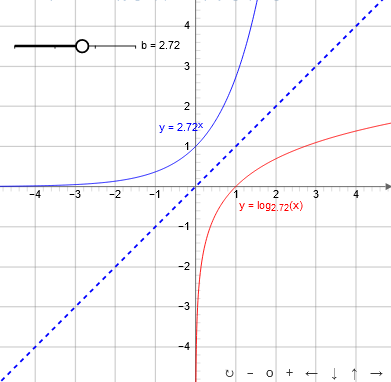
\includegraphics[width=\linewidth]{external/jsxgraph-algebra-loggraph.png}
\end{sbspanel}%
\begin{sbspanel}{0.21}%

\includegraphics[width=\linewidth]{generated/qrcode/sec_logartims-9.png}
\href{http://webwork.bridgew.edu/oer/functions_at_work/sec_logartims-9.html}{Standalone}%
\par
\href{http://webwork.bridgew.edu/oer/functions_at_work/sec_logartims-9-if.html}{Embed}%
\end{sbspanel}%
\end{sidebyside}%
\begin{paragraphs}{The Natural Logarithm for Calculus.}{subsec-naturallogs}%
Recall that the function \(y = e^x\) is called the \emph{natural exponential function}.  We call it's inverse the \terminology{natural logarithm}.%
\begin{definition}{Definition}{}{def-naturallog}%
We write \(\ln(x) = \log_e(x)\) where \(e\approx 2.718\dots\)%
\par
In other words, the \terminology{natural logarithm} \(y = \ln(x)\) is the inverse of the natural exponential function \(exp(x) = e^x\).%
\end{definition}
\begin{exploration}{Exploration}{}{ex_computingln}%
\begin{enumerate}[font=\bfseries,label=(\alph*),ref=\alph*]%
\item{}Compute \(\ln(\sqrt{e})\)%
\par\smallskip%
\noindent\textbf{\blocktitlefont Solution}.\hypertarget{ex_computingln-1-2}{}\quad{}There are two ways to answer this question.  Algebraically, we know that \(\ln\) undoes base \(e\) exponentiation.  So simply rewrite the argument of the function as a power of \(e\)%
\begin{equation*}
\ln(\sqrt{e}) = \ln(e^{1/2}) = \frac{1}{2}
\end{equation*}
%
\par
Alternatively, you can answer the question by playing the riddle game: what does the exponent \(r\) of \(e\) need to be for \(e^{r}\) to equal \(\sqrt{e}\)?%
\par
We know that \(\sqrt{e} = e^{1/2}\).  In other words, we need the exponent of \(e\) to be \(\frac{1}{2}\).  That tells us that \(\ln(\sqrt{e}) = \frac{1}{2}\)%
\item{}Compute \(\ln\left(\dfrac{1}{e}\right)\)%
\par\smallskip%
\noindent\textbf{\blocktitlefont Solution}.\hypertarget{ex_computingln-2-2}{}\quad{}Again, there are two ways to answer this question.  Algebraically, we know that \(\ln\) undoes base \(e\) exponentiation.  So simply rewrite the argument of the function as a power of \(e\)%
\begin{equation*}
\ln\left(\dfrac{1}{e}\right) = \ln(e^{-1}) = -1
\end{equation*}
%
\par
Alternatively, you can answer the question by playing the riddle game: what does the exponent \(r\) of \(e\) need to be for \(e^{r}\) to equal \(\frac{1}{e}\)?%
\par
We know that \(\frac{1}{e} = e^{-1}\).  In other words, we need the exponent of \(e\) to be \(-1\).  That tells us that \(\ln\left(\dfrac{1}{e}\right) = -1\)%
\item{}Let \(f(x) = \ln(x)\) and \(g(x) = e^x\). Simplify \(f(g(3))\), \(f(g(-2))\), \(f(g(45))\), and \(f(g(x))\)%
\par\smallskip%
\noindent\textbf{\blocktitlefont Solution}.\hypertarget{ex_computingln-3-2}{}\quad{}This is just a more complex way of asking us to simplify the natural log of e to various numbers. Reasoning as above gives%
\begin{equation*}
f(g(3)) = \ln(e^3) = 3
\end{equation*}
%
\begin{equation*}
f(g(-2)) = \ln(e^{-2}) = -2
\end{equation*}
%
\begin{equation*}
f(g(45)) = \ln(e^{45}) = 45
\end{equation*}
%
\begin{equation*}
f(g(x)) = \ln(e^{x}) = x
\end{equation*}
%
\end{enumerate}%
\end{exploration}%
\begin{assemblage}{Summary}{Key Facts.}{assemblage-naturalexplog}%
The functions \(f(x) = \ln(x)\) and \(g(x) = exp(x) = e^x\) \emph{undo} eachother.%
\begin{gather*}
\ln\left(e^x\right) = x \\
e^{\ln(x)} = x 
\end{gather*}
%
\end{assemblage}
\end{paragraphs}%
\begin{inlineexercise}{Checkpoint}{}{sec_logartims-11}%
Simplify \(e^{2\cdot \ln(5)}\).%
\par\smallskip%
\noindent\textbf{\blocktitlefont Solution}.\hypertarget{sec_logartims-11-2}{}\quad{}%
\begin{align*}
e^{2\cdot \ln(5)} = \amp e^{\ln(5)\cdot 2}      
\amp \text{ Because } a^{rs} = a^{sr}    \\
= \amp \Big(e^{\ln(5)}\Big)^2
\amp \text{ Because } a^{rs} = (a^r)^{s} \\
= \amp \Big(5\Big)^2         
\amp  \text{ Because } e^{\ln(5)} = 5     \\
= \amp 25                     
\amp 
\end{align*}
%
\end{inlineexercise}%
\end{sectionptx}
%
%
\typeout{************************************************}
\typeout{Section 6.3 Laws of Logarithms}
\typeout{************************************************}
%
\begin{sectionptx}{Section}{Laws of Logarithms}{}{Laws of Logarithms}{}{}{sec-lawsoflogs}
Logarithms have three important properties, which will play a central role in our computations.%
\begin{assemblage}{Summary}{Laws of Logarithms.}{assemblage-lawsoflogs}%
%
\begin{equation*}
\ln\Big( x^r \Big)= r\cdot \ln(x)
\end{equation*}
%
\par
%
\begin{equation*}
\ln\Big( x\cdot y \Big)= \ln(x) + \ln(y)
\end{equation*}
%
\par
%
\begin{equation*}
\ln\left( \dfrac{x}{y} \right)= \ln(x) - \ln(y)
\end{equation*}
%
\end{assemblage}
\begin{exploration}{Exploration}{}{ex_usingloglaws}%
Expand the following completely using the laws of logarithms.%
\begin{enumerate}[font=\bfseries,label=(\alph*),ref=\alph*]%
\item{}\(\ln(5^3)\)%
\par\smallskip%
\noindent\textbf{\blocktitlefont Solution}.\hypertarget{ex_usingloglaws-2-2}{}\quad{}When you look at this expression, you \emph{see} a power, so \emph{write} down the first law of logarithms \(\ln\Big( x^r \Big)= r\cdot \ln(x)\).  Using the numbers we're given, we obtain%
\begin{equation*}
\ln(5^3) = 3\cdot \ln(5)\text{.}
\end{equation*}
%
\item{}\(\ln(10\cdot 5^3) \)%
\par\smallskip%
\noindent\textbf{\blocktitlefont Solution}.\hypertarget{ex_usingloglaws-3-2}{}\quad{}When you look at this expression, you \emph{see} that the input is the product \(10\) and \(5^3\), so \emph{write} down the second law of logarithms \(\ln\Big( x\cdot y \Big)= \ln(x) + \ln(y)\).   Applying that in our example, we get%
\begin{equation*}
\ln(10\cdot 5^3) = \ln(10) + \ln( 5^3 )\text{.}
\end{equation*}
%
\par
Recopy the first logarithm \(\ln(10)\). For the second logarithm, \emph{see} that the input is a power, so \emph{write} down the first law of logarithms \(\ln\Big( x^r \Big)= r\cdot \ln(x)\).  That gives%
\begin{equation*}
\ln(10\cdot 5^3) = \ln(10) + 3\cdot \ln( 5 )\text{.}
\end{equation*}
%
\end{enumerate}%
\end{exploration}%
\alert{Warning:} Note that our three laws of logarithms only apply when the exponential, product, or fraction is \emph{inside} the logarithm.%
\par
If you try to divide logarithms, such as in \(\dfrac{\ln(5)}{\ln(2)}\), you will get something very different than our log laws. This is because of the surprising fact that%
\begin{equation*}
\log_b(x) = \dfrac{\ln(x)}{\ln(b)}
\end{equation*}
For example, if you divide   \(\dfrac{\ln(5)}{\ln(2)}\), you actually get \(\dfrac{\ln(5)}{\ln(2)} = \log_2(5) = 0.9162\dots\), which is \alert{not} the same thing as \(\ln\left(\frac{2}{5}
\right)=0.4306\dots\).%
\par
Again, for the remainder of the course, we will almost always restrict our attention to natural logarithms. But this last property is useful in many applications, and may help you remember when you can (and when you can't) perform a simplification using the laws of logarithms.%
\end{sectionptx}
%
%
\typeout{************************************************}
\typeout{Section 6.4 Solving Compound Interest for Time}
\typeout{************************************************}
%
\begin{sectionptx}{Section}{Solving Compound Interest for Time}{}{Solving Compound Interest for Time}{}{}{sec_solvingfortime}
We can now use the laws of logarithms to help us solve equations where the variable is in the exponent.%
\par
As with everything else in algebra, if we have the equation \(A = B\), we can replace it with the equation \(\ln(A) = \ln(B)\).%
\begin{exploration}{Exploration}{}{ex_solving_exponentials}%
\begin{enumerate}[font=\bfseries,label=(\alph*),ref=\alph*]%
\item{}Solve for \(x\) satisfying \(2^{3x} = 5\)%
\par\smallskip%
\noindent\textbf{\blocktitlefont Solution}.\hypertarget{ex_solving_exponentials-1-2}{}\quad{}The key idea of algebra is that if you have the equation \(A = B\), you can do the same thing to both sides and have another true equation. Here, we are given that%
\begin{equation*}
2^{3x} = 5
\end{equation*}
That means that we also know that the equation \(\ln(A) = \ln(B)\) is true, replacing \(A=2^{3x}\) and \(B=5\).  This gives%
\begin{equation*}
\ln\Big(2^{3x}\Big) = \ln\Big( 5 \Big)
\end{equation*}
We have the property of logarithms that \(\ln(x^r) = r\cdot\ln(x)\) on the left, to get the equation%
\begin{equation*}
3x \cdot \ln\Big(2\Big) = \ln\Big( 5 \Big)
\end{equation*}
Now, this looks complicated, but we can use a calculator to simplify \(\ln(2) = 0.693\dots\) and \(\ln(5) = 1.609\dots\).  This gives us the equation%
\begin{equation*}
3x \cdot 0.693{\dots} = 1.609\dots
\end{equation*}
Rearranging the left side, we have%
\begin{equation*}
3\cdot 0.693{\dots}\cdot x = 1.609\dots
\end{equation*}
Using a calculator, we see that \(3\cdot 0.693\dots = 2.079\dots\), which gives%
\begin{equation*}
2.079\dots x = 1.609\dots 
\end{equation*}
Dividing both sides by \(2.079\dots\), we get%
\begin{equation*}
x = \dfrac{1.609\dots}{2.079\dots} = 0.773\dots
\end{equation*}
You could also have done this with the original \(3x \cdot \ln\Big(2\Big) = \ln\Big( 5 \Big)\) by dividing both sides by \(3\cdot\ln(2)\) to get%
\begin{equation*}
x = \dfrac{\ln(5)}{3\cdot \ln(2)}
\end{equation*}
%
\item{}Solve for \(x\) satisfying \(4\cdot(1.95)^{2x} = 16\)%
\par\smallskip%
\noindent\textbf{\blocktitlefont Solution}.\hypertarget{ex_solving_exponentials-2-2}{}\quad{}There are two different approaches for solving an equation like this, planning ahead or using brute force.%
\begin{descriptionlist}
\begin{dlimedium}{Planning Ahead}{ex_solving_exponentials-2-2-1-1-1}%
We wish to solve the equation%
\begin{equation*}
4\cdot(1.95)^{2x} = 16
\end{equation*}
We want to eventually introduce logarithms to allow us to apply Log Law 3, to pull the \(2x\) out of the exponent. However, that law will not apply to \(4\cdot (1.95)^{2x}\) because of the coefficient of \(4\).%
\par
But we can divide both sides of the equation by 4.  This gives us%
\begin{align*}
\amp 4\cdot (1.95)^{2x} \amp = \amp 16 \amp \\
\times\frac{1}{4} \amp \amp\amp \amp \times\frac{1}{4} \\
\amp (1.95)^{2x} \amp = \amp 4 \amp 
\end{align*}
Now, we can take the logarithm of both sides%
\begin{equation*}
\ln\Big( {\color{red}(1.95)}^{\color{blue}2x} \Big) = \ln\Big( 4 \Big)
\end{equation*}
Now we can apply the law of logs \(\ln({\color{red}x}^{\color{blue}r})= {\color{blue}r}\ln({\color{red}x})\) on the left with \(\color{red} x = 1.95\) and \(\color{blue} r = 2x\)%
\begin{equation*}
{\color{blue} 2x} \cdot \ln\Big({\color{red} 1.95}\Big) = \ln\Big(4\Big)
\end{equation*}
We can now divide both sides by \(2\cdot \ln(1.95)\) to get%
\begin{equation*}
x = \dfrac{\ln\Big(4\Big)}{2\ln\Big(1.95\Big)}
\end{equation*}
This example is exact, but it can be a bit overwhelming.  You can also use your calculator to simplify%
\begin{align*}
2x \cdot \ln\Big(1.95\Big) \amp = \ln\Big(4\Big) \\
\\
2x \cdot 0.667\dots \amp = 1.386\dots \\
\\
x\cdot 1.335\dots  \amp = 1.386\dots\\
\\
x \amp = \dfrac{1.386\dots}{1.335\dots} = 1.038\dots
\end{align*}
If you do use your calculator, try to use as many decimal places as possible.  Rounding errors can grow if you do a lot of calculations.  It is possible to understand how these errors grow, but that question is beyond the scope of this course.%
\end{dlimedium}%
\begin{dlimedium}{Brute Force}{ex_solving_exponentials-2-2-1-1-2}%
We have seen how to solve this equation with a bit of planning ahead.  But what happens if you \emph{start} by taking the natural log of both sides of the quation%
\begin{equation*}
4\cdot(1.95)^{2x} = 16
\end{equation*}
You get%
\begin{equation*}
\ln\Big( {\color{red} 4}\cdot{\color{blue} (1.95)^{2x}} \Big) = \ln\Big(16\Big)
\end{equation*}
On the left side, we have \(\ln\Big( {\color{red} 4}\cdot{\color{blue} (1.95)^{2x}} \Big)\).  We \emph{cannot} use Log Law 1, since this is a product.  Instead, we need to use Log Law 2 \(\ln({\color{red} a}\cdot {\color{blue} b}) = \ln({\color{red} a}) + \ln({\color{blue} b})\) with \(\color{red} a=4\) and \(\color{blue} b=(1.95)^{2x}\).  This gives%
\begin{equation*}
\ln\Big( {\color{red} 4}\Big) + \ln\Big({\color{blue} (1.95)^{2x}} \Big) = \ln\Big(16\Big)
\end{equation*}
Now we can use Law Log 1 \(\ln(a^r) = r\cdot \ln(a)\) with \(a=1.95\) and \(r=2x\) to get%
\begin{equation*}
\ln\Big( { 4}\Big) + 2x\cdot \ln\Big({ (1.95)} \Big) = \ln\Big(16\Big)
\end{equation*}
You can simplify this using a calculator to get%
\begin{equation*}
{1.386\dots} + 2\cdot x\cdot 0.667\dots = 2.772\dots
\end{equation*}
You can solve this as usual to get%
\begin{equation*}
x = \dfrac{{2.772\dots} - 1.386\dots}{2\cdot 0.667\dots} = 1.038\dots
\end{equation*}
Alternatively, you can solve the exact equation to get%
\begin{equation*}
x = \dfrac{\ln(16) - \ln(4)}{2\cdot \ln(1.95)}
\end{equation*}
%
\end{dlimedium}%
\end{descriptionlist}
%
\item{}The balance of a certain investment is given by \(F(t) = 10\cdot 2^t\) as a function of the number of years \(t\). How long must you wait until the balance reaches 80?%
\par\smallskip%
\noindent\textbf{\blocktitlefont Solution}.\hypertarget{ex_solving_exponentials-3-2}{}\quad{}Note that \emph{this specific function} is very simple, so it is possible to answer this numerically.  After one year, the balance will be \(F(1) = 20\), after two years the balance will be \(F(2)=40\), and after three years the balance will be \(F(3)=80\).   It will take 3 years for the balance to reach \(80\).%
\par
For more complex equations, we will need to set up and solve an exponential equation.  In this case, we want to find a \(t\) such that \(F(t) = 10 \cdot 2^t\) equals 80. This gives us the equation%
\begin{align*}
80 \amp=\amp 10 \cdot 2^t \amp \\
8 \amp=\amp 2^t \amp \qquad\text{ Multiply both sides by }\dfrac{1}{10}\\
\ln\Big(8\Big) \amp=\amp \ln\Big(2^t\Big) \amp  \qquad\text{ Take }\ln\text{ of both sides}\\
\ln\Big(8\Big) \amp=\amp t\cdot \ln\Big(2\Big) \amp \qquad\text{ Log Law 1 } \ln(a^r)=r\ln(a)\\
\dfrac{\ln\Big(8\Big)}{\ln\Big(2\Big)} \amp=\amp t  \amp \qquad\text{ Divide both sides by } \ln\Big(2\Big)
\end{align*}
Alternatively, we could have simplified the natural log terms and solved as follows%
\begin{gather*}
\ln\Big(8\Big) = t\cdot \ln\Big(2\Big) \\
2.079{\dots}= t\cdot {0.693\dots} \\
t =  \dfrac{2.079{\dots}}{0.693\dots} = 3
\end{gather*}
%
\end{enumerate}%
\end{exploration}%
We can now apply these techinques to solve the equations that arise in questions of compound interest.%
\begin{exploration}{Exploration}{}{ex_compoundinterestfortime}%
You invest \textdollar{}1000 at 15\% interest compounded monthly.%
\begin{enumerate}[font=\bfseries,label=(\alph*),ref=\alph*]%
\item{}How many years are required until you double your money?%
\par\smallskip%
\noindent\textbf{\blocktitlefont Solution}.\hypertarget{ex_compoundinterestfortime-2-2}{}\quad{}First, write down the compound interest formula from  \hyperref[def-compoundinterest]{Definition~{\xreffont\ref{def-compoundinterest}}}.%
\begin{equation*}
F = P\cdot \left(1 + \frac{r}{m}\right)^{mt}
\end{equation*}
with \(P=1000\), \(r=0.15\), and \(m=12\). Furthermore, we want the \emph{future value}to be twice 1000.  In other words, we want \(F=2000\) This gives%
\begin{equation*}
2000 = 1000 \cdot \left(1 + \dfrac{0.15}{12}\right)^{12t}
\end{equation*}
Dividing both sides by 1000 gives%
\begin{equation*}
2 = \left(1 + \dfrac{0.15}{12}\right)^{12t}
\end{equation*}
%
\par
Next, we can simplify this equation using a calculator and the \hyperref[exponential-arithmetic]{properties of exponents~{\xreffont\ref{exponential-arithmetic}}}%
\par
%
\begin{align*}
2 = \amp \left(1 + \dfrac{0.15}{12}\right)^{12t} \amp \\
2 = \amp \left(\ 1.0125\ \right)^{12t} \amp \\
2 = \amp \left(\ 1.0125^{12}\ \right)^{t} \amp \qquad\text{Because } a^{rs}=(a^r)^s\\
2 = \amp \left(\ 1.16075\dots\ \right)^{t} \amp 
\end{align*}
%
\par
Finally, finish solving the exponential equation as above using the  \hyperref[assemblage-lawsoflogs]{Laws of Logs}.%
\begin{align*}
\ln\Big(2\Big) = \amp \ln\Big( \left(\ 1.16075\dots\ \right)^{t} \Big) \amp \\
\ln\Big(2\Big) = \amp t\cdot \ln\Big(  1.16075\dots \Big) \amp \qquad\text{Using }\ln(a^r) = r\ln(a)\\
t = \amp \dfrac{ \ln\Big(2\Big)}{\ln\Big(  1.16075\dots \Big) }\amp \qquad\text{Dividing both sides by }\ln\Big(  1.16075\dots \Big)\\
t = \amp 4.64\dots
\end{align*}
With 15\% interest, it will take about 4.64 years for the balance to double.%
\item{}How long will it be until the balance reaches \textdollar{}10,000?%
\par\smallskip%
\noindent\textbf{\blocktitlefont Solution}.\hypertarget{ex_compoundinterestfortime-3-2}{}\quad{}First, write down the compound interest formula%
\begin{equation*}
F = P\cdot \left(1 + \frac{r}{m}\right)^{mt}
\end{equation*}
and plug in the values we are given.  Note that we want the time when the future value \(F=10,000\).  That gives%
\begin{equation*}
10,000 = 1,000 \cdot (1 + \frac{0.15}{12})^{12t}
\end{equation*}
Simplifying this with a calculator and the laws of exponents gives%
\begin{align*}
10 \amp = (1 + \frac{0.15}{12})^{12t}\\
10 \amp = (1.0125 )^{12t}\\
10 \amp = (1.16075\dots )^{t}
\end{align*}
Taking \(\ln\) of both sides and applying the laws of logarithms, we get%
\begin{align*}
\ln\Big(10\Big) \amp = \ln\Big( (1.16075\dots )^{t} \Big)\\
\ln\Big(10\Big) \amp = t\cdot \ln\Big( 1.16075\dots  \Big)\\
\dfrac{\ln\Big(10\Big)}{\ln\Big( 1.16075\dots  \Big)} \amp = t  \\
t \amp = 14.868\dots \amp 
\end{align*}
The balance will increase to \textdollar{}10,000 in about 15 years.%
\end{enumerate}%
\end{exploration}%
As an exercise, find how long it takes for a balance of \textdollar{}1000 to double at 2\% interest, at 5\% interest, and at 30\% interest.%
\par
For our last application, we will return to the concept of \terminology{depreciation}, discussed in more depth in \hyperref[insight-depreciation]{Application~{\xreffont\ref{insight-depreciation}}} and \hyperref[ex_depreciation1]{Exploration~{\xreffont\ref{ex_depreciation1}}}%
\begin{exploration}{Exploration}{}{ex_depreciation2}%
Suppose that a certain asset loses 30\% of its value each year. In other words, suppose that the value of the asset after \(t\) years is given by%
\begin{equation*}
V(t) = P\cdot (1-0.3)^t
\end{equation*}
%
\begin{enumerate}[font=\bfseries,label=(\alph*),ref=\alph*]%
\item{}Suppose that  the asset starts with value \(P=1000\). Find the value after 12 years.%
\par\smallskip%
\noindent\textbf{\blocktitlefont Solution}.\hypertarget{ex_depreciation2-2-2}{}\quad{}The future value function is%
\begin{equation*}
V(t) = 1000 \cdot (1-0.3)^t = 1000\cdot 0.7^t
\end{equation*}
After \(12\) years,%
\begin{equation*}
V(12) = 1000 \cdot (1-0.3)^{12} = 13.841
\end{equation*}
After \(12\) years, the value of the asset will be approximately \textdollar{}13.84%
\item{}Suppose that the value after 12 years is \textdollar{}50.  Find the starting value \(P\).%
\par\smallskip%
\noindent\textbf{\blocktitlefont Solution}.\hypertarget{ex_depreciation2-3-2}{}\quad{}The future value function is%
\begin{equation*}
V = P \cdot (1-0.3)^t 
\end{equation*}
We know that when \(t=12\), that \(V=50\).  Plugging this in gives%
\begin{align*}
50 \amp = P \cdot (1-0.3)^{12}\\
50 \amp = P \cdot 0.0138\dots\\
\frac{50}{0.138} \amp = P\\
P \amp = 3612.380\dots
\end{align*}
The starting value must have been about \textdollar{}3,612.38%
\item{}Suppose that the asset starts with a value \(P=1000\). Find the number of years \(t\) for the value to decrease to \(100\).%
\par\smallskip%
\noindent\textbf{\blocktitlefont Solution}.\hypertarget{ex_depreciation2-4-2}{}\quad{}The future value function is%
\begin{equation*}
V = P \cdot (1-0.3)^t 
\end{equation*}
We want the time \(t\) when the value reaches \(V=100\) when from a starting value of \(P=1,000\).  Plugging this in gives%
\begin{align*}
100 \amp = 1000 \cdot (0.7)^t\\
0.1 \amp =  (0.7)^t\\
\ln\Big(0.1\Big) \amp =  \ln\Big((0.7)^t\Big)\\
\ln\Big(0.1\Big) \amp =  t\cdot \ln\Big(0.7\Big)\\
t \amp = \dfrac{ \ln\Big(0.1\Big)}{\ln\Big(0.7\Big)} = 6.45\dots
\end{align*}
It will take about 6.45 years for the balance to decline from 1000 to 100.%
\end{enumerate}%
\end{exploration}%
\begin{insight}{Application}{Depreciating Assets and Scrap Value.}{sec_solvingfortime-10}%
In this class, our focus is on the mathematical tools that underly economics, business, and accounting.%
\par
In accounting, you will learn about how to decide which mathematical too to use (straight line versus declining balance depreciation), and to find a numerical value for the rate of depreciation.%
\par
Rates of depreciation can be found in many ways. For example, you can use the actual sales price for cars based on their mileage to emperically determine how much the value drops per mile.%
\par
But there are also other ways of calculating the rate of depreciation. For example, some assets have a known or conventional "scrap value" and "expected lifespan."%
\par
Once you know the starting value, the scrap value, and the expected lifespan, you can actually compute the yearly depreciation you should use. Mathematically, that means solving%
\begin{equation*}
F = P ( 1- r)^t
\end{equation*}
for the rate \(r\) to get%
\begin{equation*}
r = 1- \sqrt[t]{\frac{F}{P}}
\end{equation*}
%
\end{insight}
\begin{sidebyside}{2}{0.075}{0.075}{0.17}%
\begin{sbspanel}{0.47}%
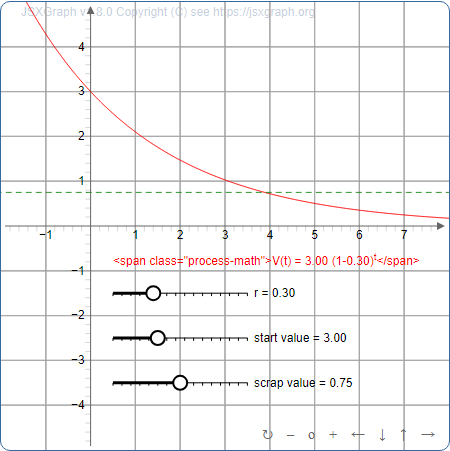
\includegraphics[width=\linewidth]{generated/preview/interactive_depreciation-preview.png}
\end{sbspanel}%
\begin{sbspanel}{0.21}%

\includegraphics[width=\linewidth]{generated/qrcode/interactive_depreciation.png}
\href{http://webwork.bridgew.edu/oer/functions_at_work/interactive_depreciation.html}{Standalone}%
\par
\href{http://webwork.bridgew.edu/oer/functions_at_work/interactive_depreciation-if.html}{Embed}%
\end{sbspanel}%
\end{sidebyside}%
\end{sectionptx}
%
%
\typeout{************************************************}
\typeout{Section 6.5 Applications of Logarithms}
\typeout{************************************************}
%
\begin{sectionptx}{Section}{Applications of Logarithms}{}{Applications of Logarithms}{}{}{sec-logapplications}
Although logarithms are less familiar than lines, polynomials, and rational functions, they do play an important role in the physical and economic sciences.  In this section we will introduce two examples of logarithms. These examples are somewhat simplified for mathematical clarity, but the interested reader is encouraged to continue their study to understand the relevant nuances.%
\par
Logarithmic models often arise when discussing quantities that are more meaningful when compared to a baseline than when viewed as isolated numbers.%
\par
For example, it is hard to say how happy it would make someone to win a \textdollar{}1000 prize. Presumably this win would make someone with \textdollar{}5,000 in their bank account would be much happier than a similar win would make someone with \textdollar{}5,000,000 in wealth.%
\par
Similarly, a cell phone ringer might seem very loud in a quiet library, but the same ringer would sound very quiet at a packed concert.%
\begin{exploration}{Exploration}{Sound Perception and Logarithms.}{sec-logapplications-6}%
Let \(x\) denote the magnitude of a sound, measured by the amplitude of the sound wave itself. The \emph{percieved sound level} is given by%
\begin{equation*}
dB(x) = 10\cdot \log_{10}(x)
\end{equation*}
%
\begin{aside}{Aside}{}{sec-logapplications-6-2-2}%
This formula is a slight oversimplificaiton.  See, for example, \href{https://en.wikipedia.org/wiki/Decibel\#Perception}{Wikipedia}\footnotemark{} for more details.%
\end{aside}
\begin{enumerate}[font=\bfseries,label=(\alph*),ref=\alph*]%
\item{}The sound waves of rustling leaves have power \(x=100\). Find \(dB(100)\).%
\par\smallskip%
\noindent\textbf{\blocktitlefont Solution}.\hypertarget{sec-logapplications-6-3-2}{}\quad{}\(dB(100)=10\cdot\log_{10}(100) = 10\cdot\log_{10}(10^2)  = 20\) decibels%
\item{}The sound waves in a quiet library have power \(10,000\). Find \(dB(10,000)\). How much louder does this sound compared to rustling leaves?%
\par\smallskip%
\noindent\textbf{\blocktitlefont Solution}.\hypertarget{sec-logapplications-6-4-2}{}\quad{}\(dB(10,000)=10\cdot\log_{10}(10,000) = 10\cdot\log_{10}(10^4) = 40\) decibels.%
\par
The decibel rating of a quiet library (40 dB) is twice the decibel rating of leaves (20 dB), so the library sounds twice as loud.%
\par
But surprisingly, this apparent doubling is actually the result of a \(\frac{10,000}{100}=100\)-fold increase in the power of the waves.%
\item{}The sound waves from an alarm clock have power \(100,000,000\). Find \(dB(100,000,000)\). How much louder does this sound compared to a quiet library?%
\par\smallskip%
\noindent\textbf{\blocktitlefont Solution}.\hypertarget{sec-logapplications-6-5-2}{}\quad{}\(dB(100,000,000)=10\cdot\log_{10}(100,000,000) = 10\cdot\log_{10}(10^8) = 80\) decibels.%
\par
The decibel rating of an alarm clock (80 dB) is twice the decibel rating of a quiet library (40 dB), so the library sounds twice as loud.%
\par
But surprisingly, this apparent doubling is actually the result of a \(\frac{100,000,000}{10,000}=10,000\)-fold increase in the power of the waves.%
\item{}How much does doubling the power of the sound waves increase the decibel rating of a given frequency \(x\)?%
\par\smallskip%
\noindent\textbf{\blocktitlefont Solution}.\hypertarget{sec-logapplications-6-6-2}{}\quad{}We want to understand the decibel rating of \(2x\). Using the definition of \(dB\) gives%
\begin{align*}
dB(2x) \amp = 10 \log_{10}(2x) \amp \\
\amp = 10\Big(\log_{10}(2) + \log_{10}(x)\Big) \amp \ln(ab)=\ln(a)+\ln(b)\\
\amp = 10\Big(0.301029 + \log_{10}(x)\Big) \amp \text{calculator}\\
\amp = 3.01029 + 10\log_{10}(x)  \amp \\
\amp = 3.01029 + dB(x)  \amp 
\end{align*}
Doubling the power of the sound waves only increases the decibel rating by about \(3dB\)%
\item{}How much does increasing the power of the sound waves by a factor of 100 change the decibel rating of a given frequency \(x\)?%
\par\smallskip%
\noindent\textbf{\blocktitlefont Solution}.\hypertarget{sec-logapplications-6-7-2}{}\quad{}We want to understand the decibel rating of \(100x\). Using the definition of \(dB\) gives%
\begin{align*}
dB(10x) \amp = 100 \log_{10}(10x) \amp \\
\amp = 10\Big(\log_{100}(10) + \log_{10}(x)\Big) \amp \ln(ab)=\ln(a)+\ln(b)\\
\amp = 10\Big(2 + \log_{10}(x)\Big) \amp \text{calculator}\\
\amp = 20 + 10\log_{10}(x)  \amp \\
\amp = 20 + dB(x)  \amp 
\end{align*}
\emph{Multiplying the power of sound waves by a factor of \(100\)} only increases the decibel rating by the \emph{addition of \(20dB\)}.%
\end{enumerate}%
\end{exploration}%
\footnotetext[1]{\nolinkurl{en.wikipedia.org/wiki/Decibel\#Perception}\label{sec-logapplications-6-2-2-1-2}}%
\begin{exploration}{Exploration}{Utility and Logarithms.}{sec-logapplications-7}%
Some economists argue that the \emph{percieved value of money} (often called the \emph{utility} of money) is logarithmic. Of course, different people will have different utility functions. To see why, we will explore a specific utility function.%
\begin{aside}{Aside}{}{sec-logapplications-7-2-2}%
You can find more on this in Chapter 25 of \emph{Thinking Fast and Slow}. %
\end{aside}
Given \emph{life savings} of money \(x\) in dollars, let the utility of \textdollar{}\(x\) of these savings be given by%
\begin{equation*}
U(x) = 21.7\ln(x) + 150
\end{equation*}
%
\begin{enumerate}[font=\bfseries,label=(\alph*),ref=\alph*]%
\item{}Find the utility of \textdollar{}0, \textdollar{}10, \textdollar{}100, \textdollar{}1000, \textdollar{}10,000, \textdollar{}100,000, and \textdollar{}1,000,000.%
\par
Explain the meaning of these numbers.  Why are some negative? Why are some positive?  How do they change as your life savings increases?%
\par\smallskip%
\noindent\textbf{\blocktitlefont Solution}.\hypertarget{sec-logapplications-7-3-2}{}\quad{}%
\begin{equation*}
\begin{array}{c|c|c|c|c|c|c|c}
\text{dollars }x         
&  0 
&  10   
&  100  
&  1,000  
&  10,000 
&  100,000
&  1,000,000
\\ \hline
\text{utility }U(x)
& DNE
& -100.0	
& -50.06
& -0.10
& 49.86
& 99.83
& 149.79
\end{array}
\end{equation*}
The first thing to note is that \(U(0)\) is undefined.  Mathematically, this is because \(\ln(0)\) is undefined.  Practically, this is because you would be \emph{very} unhappy if you did not have any money to use to pay rent, buy food, etc.%
\par
Next, note that this person has negative utility until approximately \(x=1,000\).  Perhaps this would mean that the individual needs at least \textdollar{}1000 for basic necessities.  Then a balance of less than \textdollar{}1000 implies unmet necesseties, which would make the individual unhappy indeed.%
\par
Finally, consider the values above \textdollar{}1000.  Note that increasing the balance by a factor of 10 \emph{approximately} increases their happiness by 50 utility points. Often, this is because the individual will start with a list of very clear and very productive uses of the money.  As those clear producive uses are taken care of, the individual needs to look for less clear or less productive uses for their money.  Thus, each dollar does not have the same value to the individual!%
\par
Of course, this is an overly simplified example.  In fact, utility functions are much more complex.  But even these more complex functions will share many of the above properties with our logarithmic utility.%
\item{}How does doubling a wealth of \textdollar{}\(x\) impact utility?%
\par\smallskip%
\noindent\textbf{\blocktitlefont Solution}.\hypertarget{sec-logapplications-7-4-2}{}\quad{}We are asked to understand the utility of \textdollar{}\(2x\) dollars.  Using the utility function given, we have%
\begin{align*}
U(2x) \amp = 21.7\ln(2x) + 150 \amp \\
\amp = 21.7\Big(\ln(2) + \ln(x) \Big) + 150 \amp \ln(ab)=\ln(a)+\ln(b) \\
\amp = 21.7\ln(2) + 21.7\ln(2x) + 150 \amp \\
\amp = 15.04 + 21.7\ln(2x) + 150 \amp \\
\amp = 15.04 + U(x) \amp 
\end{align*}
\emph{Doubling} the amount of money available \emph{adds} 15.04 utility (or "happiness") points.%
\item{}How does multiplying a wealth of \textdollar{}\(x\) by a factor of 10 impact utility?%
\par\smallskip%
\noindent\textbf{\blocktitlefont Solution}.\hypertarget{sec-logapplications-7-5-2}{}\quad{}We are asked to understand the utility of \textdollar{}\(10x\) dollars.  Using the utility function given, we have%
\begin{align*}
U(10x) \amp = 21.7\ln(10x) + 150 \amp \\
\amp = 21.7\Big(\ln(10) + \ln(x) \Big) + 150 \amp \ln(ab)=\ln(a)+\ln(b) \\
\amp = 21.7\ln(10) + 21.7\ln(x) + 150 \amp \\
\amp = 49.97 + 21.7\ln(x) + 150 \amp \\
\amp = 49.97 + U(x) \amp 
\end{align*}
\emph{Multipling by 10} the amount of money available \emph{adds} 49.97 utility (or "happiness") points.%
\end{enumerate}%
\end{exploration}%
\end{sectionptx}
\end{chapterptx}
\end{partptx}
%
%
\typeout{************************************************}
\typeout{Part II Change and Rates}
\typeout{************************************************}
%
\begin{partptx}{Part}{Change and Rates}{}{Change and Rates}{}{}{part-rates}
\renewcommand*{\partname}{Part}
 %
%
\typeout{************************************************}
\typeout{Chapter 7 Limits}
\typeout{************************************************}
%
\begin{chapterptx}{Chapter}{Limits}{}{Limits}{}{}{ch_limits}
\renewcommand*{\chaptername}{Chapter}
\begin{introduction}{}%
%
\end{introduction}%
%
%
\typeout{************************************************}
\typeout{Section 7.1 Reading Graphs Dynamically}
\typeout{************************************************}
%
\begin{sectionptx}{Section}{Reading Graphs Dynamically}{}{Reading Graphs Dynamically}{}{}{sec_readingdynamically}
Reading graphs \emph{dynamically} will be an essential part of understanding the key concepts of calculus, and applying those concepts to your daily life.%
\par
To read any graph dynamically, start at a specific \(x\) value, and imagine "standing" on the function above that point on the x-axis. The \(y\) value corresponds with your height above the x-axis.%
\par
Next, imagine walking right (increasing \(x\)) and left (decreasing \(x\)) along the curve. As you walk, the curve \emph{forces} your height to move up or down.%
\begin{figureptx}{Figure}{}{figure_interactivelimit}{}%
\begin{sidebyside}{2}{0.075}{0.075}{0.17}%
\begin{sbspanel}{0.47}%
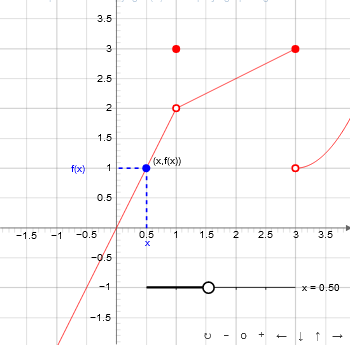
\includegraphics[width=\linewidth]{external/jsxgraph-limitpicewise.png}
\end{sbspanel}%
\begin{sbspanel}{0.21}%

\includegraphics[width=\linewidth]{generated/qrcode/figure_interactivelimit-2.png}
\href{http://webwork.bridgew.edu/oer/functions_at_work/figure_interactivelimit-2.html}{Standalone}%
\par
\href{http://webwork.bridgew.edu/oer/functions_at_work/figure_interactivelimit-2-if.html}{Embed}%
\end{sbspanel}%
\end{sidebyside}%
\tcblower
\end{figureptx}%
\begin{example}{Example}{Exploring Figure~{\xreffont\ref*{figure_interactivelimit}}.}{example_interactivelimit_intuitive}%
Let's explore what happens in  \hyperref[figure_interactivelimit]{Figure~{\xreffont\ref{figure_interactivelimit}}}.%
%
\begin{itemize}[label=\textbullet]
\item{}To see what happens as you \emph{approach \(x=1\) from the left},%
\begin{enumerate}
\item{}Move the \(x\) value to some number less than \(1\). For simplicity, start by moving to \(x=0\). At that point on the curve, your height will be \(y=0\).%
\item{}Drag the slider to increase \(x\) towards 1, making sure never to allow \(x\) to equal 1.%
\par
As you increased \(x\) (as you move it right), you will have seen the height increase as well.  Even more, you will have seen the height getting closer and closer to \(y=2\).%
\item{}Because of this, we say that your height \(y=f(x)\) gets closer and closer to \(y=2\) as \(x\) approaches 1 from the left.%
\end{enumerate}
%
\par
\alert{Important:} The fact that \(f(1)=3\) is unrelated to our question, because that tells us what happens \emph{at that point}, not what happens \emph{during the process of approaching that point}.%
\item{}To see what happens as you \emph{approach \(x=1\) from the right},%
\begin{enumerate}
\item{}Move the slider so that \(x\) is significantly bigger than \(2\). For simplicity, start by moving to \(x=2\). At that point on the curve, your height will be \(y=2.5\).%
\item{}Drag the slider to \emph{decrease} \(x\) toward 1, making sure never to allow \(x\) to equal 1. As you do this, the height decreases, getting closer and closer to \(2\).%
\item{}Because of this, we say that the height \(y=f(x)\) gets closer and closer to \(y=2\) as \(x\) approaches 1 from the right.%
\end{enumerate}
%
\item{}As you approach \(x=3\) from the left, your height increases to \(y=3\).%
\par
As you approach \(x=3\) from the right, your height decreases to \(y=1\).%
\end{itemize}
\end{example}
To answer these questions clearly and concisely, we need new mathematical language. To understand our notation, it will be helpful to remember the number line. If you (\(x\)) approach a number \(a\) \terminology{from the left}, you are approaching \(a\) from the side of the number line with all the negative numbers. Because of that, we write \(x\rightarrow a^-\) as a shorthand for \emph{approaches \(a\) from the left}. \begin{image}{0.335}{0.33}{0.335}{}%
\resizebox{\linewidth}{!}{%
\begin{tikzpicture}
  \draw[axes] (-0.5,0) -- (3.5,0); 
  \foreach \x in {0,0.5,...,3}
    \draw (\x,-0.05)--(\x,0.05);
  \node[below,circle] at (1.5,0) {$a$};
  \node[below,circle,draw] (x) at (0.5,0) {$x$};
  \draw[-latex] (x.east) to ++ (0.5,0);
  \node at (-1,0) {\color{blue}\Large $\mathbf{-}$};
  \node at (4,0) {$+$};
\end{tikzpicture}
}%
\end{image}%
 If you (\(x\)) approach a number \(a\) \terminology{from the right}, you are approaching \(a\) from the side of the number line with all the positive numbers. Because of that, we write \(x\rightarrow a^+\) as a shorthand for \emph{approaches \(a\) from the right}. \begin{image}{0.335}{0.33}{0.335}{}%
\resizebox{\linewidth}{!}{%
\begin{tikzpicture}
  \draw[axes] (-0.5,0) -- (3.5,0); 
  \foreach \x in {0,0.5,...,3}
    \draw (\x,-0.05)--(\x,0.05);
  \node[below,circle] at (1.5,0) {$a$};
  \node[below,circle,draw] (x) at (2.5,0) {$x$};
  \draw[-latex] (x.west) to ++ (-0.5,0);
  \node at (-1,0) {$-$};
  \node at (4,0) {\color{blue}\Large $\mathbf{+}$};
\end{tikzpicture}
}%
\end{image}%
%
\begin{definition}{Definition}{}{def-limit}%
Suppose that \(f(x)\) is some function, and that \(a\) and \(L\) are two numbers.%
%
\begin{descriptionlist}
\begin{dlimedium}{Left}{def-limit-1-2-1}%
Suppose that is \(x\) approaching \(a\) from the left (that \(x\rightarrow a^-\)). If the heights \(f(x)\) get closer and closer to a number \(L\), then we say that the the \terminology{left hand limit} exists, and write%
\begin{equation*}
\lim_{x\rightarrow a^-} f(x) = L
\end{equation*}
We can read this expression by saying "(1) the limit (2) as \(x\) approaches \(a\) from the left is (3) equal to "L".%
\end{dlimedium}%
\begin{dlimedium}{Right}{def-limit-1-2-2}%
Suppose that is \(x\) approaching \(a\) from the right (that \(x\rightarrow a^+\)). If the heights \(f(x)\) get closer and closer to a number \(L\), then we say that the the \terminology{right hand limit} exists, and write%
\begin{equation*}
\lim_{x\rightarrow a^+} f(x) = L
\end{equation*}
We can read this expression by saying "(1) the limit (2) as \(x\) approaches \(a\) from the right is (3) equal to "L".%
\end{dlimedium}%
\begin{dlimedium}{Undirected}{def-limit-1-2-3}%
Sometimes, we talk about limits without any direction.%
\par
We say that the (undirected) \terminology{limit} of \(f(x)\) as \(x\) approaches \(a\) is equal to \(L\), written%
\begin{equation*}
\lim_{x\rightarrow a} f(x) = L
\end{equation*}
if  as the \emph{input \(x\)} gets \emph{closer to \(a\)}, the \emph{output \(f(x)\)} gets \emph{closer to \(L\)}.%
\end{dlimedium}%
\end{descriptionlist}
\end{definition}
\begin{exploration}{Exploration}{}{sec_readingdynamically-9}%
Let \(f(x)\) be the function defined by the graph in \hyperref[figure_interactivelimit]{Figure~{\xreffont\ref{figure_interactivelimit}}}. Compute the following limits.%
\begin{enumerate}[font=\bfseries,label=(\alph*),ref=\alph*]%
\item{}\(\displaystyle \lim_{x\rightarrow 1^-} f(x)\)%
\par\smallskip%
\noindent\textbf{\blocktitlefont Answer}.\hypertarget{sec_readingdynamically-9-2-2}{}\quad{}Following the reasoning from \hyperref[example_interactivelimit_intuitive]{Example~{\xreffont\ref{example_interactivelimit_intuitive}}}, we see that \(\displaystyle \lim_{x\rightarrow 1^-} f(x)=2\)%
\item{}\(\displaystyle \lim_{x\rightarrow 1^+} f(x)\)%
\par\smallskip%
\noindent\textbf{\blocktitlefont Answer}.\hypertarget{sec_readingdynamically-9-3-2}{}\quad{}Following the reasoning from \hyperref[example_interactivelimit_intuitive]{Example~{\xreffont\ref{example_interactivelimit_intuitive}}}, we see that \(\lim_{x\rightarrow 1^+} f(x)=2\)%
\item{}\(\displaystyle \lim_{x\rightarrow 1} f(x)\)%
\par\smallskip%
\noindent\textbf{\blocktitlefont Answer}.\hypertarget{sec_readingdynamically-9-4-2}{}\quad{}We have seen that as \(x\) approaches 1, the height goes to 2 \emph{regardless} of the direction.  That tells us that the undirected limit exists and equals 2.  In other words, \(\lim_{x\rightarrow 1} f(x)=2\)%
\item{}\(\displaystyle \lim_{x\rightarrow 3^-} f(x)\)%
\par\smallskip%
\noindent\textbf{\blocktitlefont Answer}.\hypertarget{sec_readingdynamically-9-5-2}{}\quad{}Following the reasoning from \hyperref[example_interactivelimit_intuitive]{Example~{\xreffont\ref{example_interactivelimit_intuitive}}}, we see that \(\lim_{x\rightarrow 3^-} f(x)=3\)%
\item{}\(\displaystyle \lim_{x\rightarrow 3^+} f(x)\)%
\par\smallskip%
\noindent\textbf{\blocktitlefont Answer}.\hypertarget{sec_readingdynamically-9-6-2}{}\quad{}Following the reasoning from \hyperref[example_interactivelimit_intuitive]{Example~{\xreffont\ref{example_interactivelimit_intuitive}}}, we see that \(\lim_{x\rightarrow 3^+} f(x)=1\)%
\item{}\(\displaystyle \lim_{x\rightarrow 3} f(x)\)%
\par\smallskip%
\noindent\textbf{\blocktitlefont Answer}.\hypertarget{sec_readingdynamically-9-7-2}{}\quad{}We have seen that as \(x\) approaches 3, the height goes to \emph{different values} depending on your direction of approach.  That tells us that the undirected limit \emph{does not exist}.  In other words, \(\lim_{x\rightarrow 3} f(x)= DNE\)%
\end{enumerate}%
\end{exploration}%
In the graph above, we have already seen that as we move the input (slider) \(x\) closer to \(1\), that the height (output) gets closer to \(2\).  In our new lanugage, that says%
\begin{equation*}
\lim_{x\rightarrow 1} f(x) = 2
\end{equation*}
%
\begin{note}{Note}{A little extra precision.}{sec_readingdynamically-11}%
In this class, we only need an informal understanding of limits, and the definitions above should be more than enough.%
\par
But there is still a little bit of ambiguity in expressions like "getting closer and closer to."  It is natural to ask, how close is close enough? The answer to that question gives us the full, mathematical definition of a limit.%
\par
That definition says that \(\lim_{x\rightarrow a}f(x) = L\) if and only if for \emph{any} acceptable error \(\varepsilon>0\), there is an acceptable distance \(d>0\) such that the difference between the actual height \(f(x)\) and the limit height of \(L\) is less than \(\varepsilon\) whenever the input \(x\) is no more than distance \(d\) from the point \(a\) that you are approaching.%
\par
Again, unless you find it helpful we don't need that more formal definition for this class.  The main point is that it is possible to eliminate any ambiguity about what "close enough" really means.%
\end{note}
The function in Figure \hyperref[figure_interactivelimit]{Figure~{\xreffont\ref{figure_interactivelimit}}} is very unusual. Most mathematical functions can be drawn smoothly, with one or two strokes of a pen. But this function includes lots of jumping around, and we need to lift the pen every time there is a "jump". We can make this precise using the following definition.%
\begin{definition}{Definition}{}{def-continuous}%
We say that a function \(f(x)\) is \terminology{continuous} on its domain if you can draw the graph of the function without lifting your pen.%
\par
A function is \terminology{continuous at the number \(a\)} if%
\begin{equation*}
\lim_{x\rightarrow a} f(x) = f(a)\text{,}
\end{equation*}
which means that both the left and right limits exist, and equal the value that \(f\) achieves at \(a\).%
\end{definition}
The two definitions are really two ways of saying the same thing. If your function can be drawn without lifting your pen, then each point flows smoothly into the next point, and the limit \(\lim_{x\rightarrow a} f(x) \) exists and equals \(f(a)\)%
\par
On the other hand, if the function can't be drawn without lifting your pen, then there must be some point in drawing the curve where the function does \emph{not} smoothly flow into the next point.  In that case, the limit \(\lim_{x\rightarrow a}f(x)\) either does not exist, or it does not equal \(f(a)\).%
\begin{example}{Example}{Three reasons  a function might \emph{not} be continuous..}{sec_readingdynamically-16}%
%
\begin{descriptionlist}
\begin{dlimedium}{Removable Discontinuity}{sec_readingdynamically-16-2-1}%
\begin{image}{0.25}{0.5}{0.25}{}%
\resizebox{\linewidth}{!}{%
\begin{tikzpicture}
  \draw[axes] (-1,0) -- (3,0);
  \draw[axes] (0,-1) -- (0,3);
  \draw [curve,domain=0.5:2.5] plot ({\x},{\x });
  \draw[fill=white] (1.5,1.5) circle (3pt);
  \draw[fill] (1.5,0.5) circle (3pt);
\end{tikzpicture}
}%
\end{image}%
 Imagine running along this graph. The discontinuity is a hole in the ground, like an open manhole cover. If you were to walk over that hole, you would fall down the hole, and hit the ground at the bottom. But it seems like someone should be able to \terminology{remove} this discontinuity by covering up the manhole cover (by redefining the function at that specific point).%
\par
We say that \emph{any} function has a \terminology{removable discontinuity} if the left and right limits both exist, and both equal the same number, but if that number is not equal to \(f(a)\).%
\end{dlimedium}%
\begin{dlimedium}{Jump Discontinuity}{sec_readingdynamically-16-2-2}%
\begin{image}{0.25}{0.5}{0.25}{}%
\resizebox{\linewidth}{!}{%
\begin{tikzpicture}
  \draw[axes] (-1,0) -- (3,0);
  \draw[axes] (0,-1) -- (0,3);
  \draw[curve,domain=0.5:1.5] plot ({\x},{\x });
  \draw[curve,domain=1.5:2.5] plot ({\x},{\x + 1});
  \draw[fill=white] (1.5,1.5) circle (3pt);
  \draw[fill] (1.5,2.5) circle (3pt);
\end{tikzpicture}
\qquad
}%
\end{image}%
 In this graph, the limit does not exist.  If you imagine running along this curve, you would need to \terminology{jump} to get from one side of the discontinuity to the other.%
\par
We say that \emph{any} function has a \terminology{jump discontinuity} if the left and right limits equal two different finite numbers.%
\end{dlimedium}%
\begin{dlimedium}{Infinite Discontinuity}{sec_readingdynamically-16-2-3}%
\begin{image}{0.25}{0.5}{0.25}{}%
\resizebox{\linewidth}{!}{%
\begin{tikzpicture}
  \draw[axes] (-1,0) -- (3,0);
  \draw[axes] (0,-1) -- (0,3);
  \draw [curve,domain=-0.5:1.33] plot ({\x},{0.5/abs(\x - 1.5)});
  \draw [curve,domain=1.67:3] plot ({\x},{0.5/abs(\x - 1.5)});
  \draw[dashed] (1.5,-1)--(1.5,3.1);
\end{tikzpicture}
}%
\end{image}%
 In this graph, the left and right limits both go off to infinity, and the graph of the function has a vertical asymptote. If you imagine running along this curve, you would need to be able to go to infinity in the process of getting from one side to the other.%
\par
We say that \emph{any} function has an \terminology{infinite discontinuity} if either the left or right limit goes to infinity.%
\end{dlimedium}%
\end{descriptionlist}
\end{example}
\end{sectionptx}
%
%
\typeout{************************************************}
\typeout{Section 7.2 Macroeconomics and Mostly Continuous Functions}
\typeout{************************************************}
%
\begin{sectionptx}{Section}{Macroeconomics and Mostly Continuous Functions}{}{Macroeconomics and Mostly Continuous Functions}{}{}{sec-econlimits}
There is an important difference between histograms and scatter plots on the one hand, and continuous functions on the other. \begin{image}{0}{1}{0}{}%
\resizebox{\linewidth}{!}{%
\begin{tikzpicture}
  \draw[-latex] (0,0) -- (0,4);
  \draw[-latex] (0,0) -- (5,0);

  \filldraw (1,3) circle (3pt);
  \filldraw (2,2) circle (3pt);
  \filldraw (3,1) circle (3pt);
  \filldraw (4,2) circle (3pt);

  \node at (2.5,-1) {A few discrete points};
\end{tikzpicture}
\qquad
\begin{tikzpicture}
  \draw[-latex] (0,0) -- (0,4);
  \draw[-latex] (0,0) -- (5,0);

  \filldraw (1,3) circle (1pt);
  \filldraw (1.25,2.75) circle (1pt);
  \filldraw (1.5,2.5) circle (1pt);
  \filldraw (1.75,2.25) circle (1pt);
  \filldraw (2,2) circle (1pt);
  \filldraw (2.25,1.7) circle (1pt);
  \filldraw (2.5,1.4) circle (1pt);
  \filldraw (2.75,1.125) circle (1pt);
  \filldraw (3,1) circle (1pt);
  \filldraw (3.25,1.125) circle (1pt);
  \filldraw (3.5,1.4) circle (1pt);
  \filldraw (3.75,1.675) circle (1pt);
  \filldraw (4,2) circle (1pt);								


  \node at (2.5,-1) {Many discrete points};
\end{tikzpicture}
\qquad

\begin{tikzpicture}
  \draw[-latex] (0,0) -- (0,4);
  \draw[-latex] (0,0) -- (5,0);

  \draw [curve, smooth] plot coordinates
        {
            (1,3)
            (2,2)
            (3,1)
            (4,2)
        };
  \node at (2.5,-1) {A continuous curve};
\end{tikzpicture}
}%
\end{image}%
 In a discrete graph, you would need to "jump" to move between the discrete points. But as you add more and more points, the distance you would need to "jump" gets smaller and smaller. If you add enough discrete points, the graph becomes indistinguishable from a \emph{continuous} curve, where you can walk smoothly along the curve.%
\par
In the words of \href{https://www.investopedia.com/terms/m/macroeconomics.asp}{Investopedia}\footnote{\nolinkurl{www.investopedia.com/terms/m/macroeconomics.asp}\label{sec-econlimits-3-2}}, ``Macroeconomics is the branch of economics that deals with the structure, performance, behavior, and decision-making of the whole, or aggregate, economy''.%
\par
There are a \emph{lot} of data points in the overall economy, so many macroeconomic functions are essentially continuous. However, certain unique events can introduce jumps.%
\par
As a very simplified example, any given oil rig will be able to produce different amounts of oil, based on how many people are working on it, how much electricity is used for the pump, and other factors. These factors can generally be scaled smoothly, so the cost of producing oil should be roughly continuous as a function of the number of barrels to be produced.%
\par
But there are also limits to the amount of oil that a certain rig will be able to extract.  To produce more than that amount of oil, an entirely new oil rig will need to be set up, causing a massive jump in the cost. Furthermore, additional refinement will probably be needed after the new rig is produced, possibly resulting in another jump in cost.%
\begin{exploration}{Exploration}{}{explore_oillimit_graphical}%
Suppose that the following graph shows the cost \(C\) in millions of dollars of producing \(x\) million barells of oil at a specific oil field. Use this graph to answer the following questions.%
\begin{sidebyside}{2}{0.075}{0.075}{0.17}%
\begin{sbspanel}{0.47}%
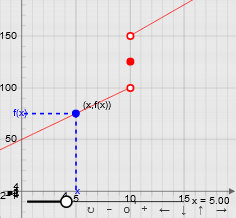
\includegraphics[width=\linewidth]{external/jsxgraph-figure_oillimit.png}
\end{sbspanel}%
\begin{sbspanel}{0.21}%

\includegraphics[width=\linewidth]{generated/qrcode/explore_oillimit_graphical-1-2.png}
\href{http://webwork.bridgew.edu/oer/functions_at_work/explore_oillimit_graphical-1-2.html}{Standalone}%
\par
\href{http://webwork.bridgew.edu/oer/functions_at_work/explore_oillimit_graphical-1-2-if.html}{Embed}%
\end{sbspanel}%
\end{sidebyside}%
\begin{enumerate}[font=\bfseries,label=(\alph*),ref=\alph*]%
\item{}Compute \(\lim_{x\rightarrow 10^-}C(x).\) What does this tell us about oil production?%
\par\smallskip%
\noindent\textbf{\blocktitlefont Solution}.\hypertarget{explore_oillimit_graphical-2-2}{}\quad{}As the number of (millions of) gallons of oil increases to 10 from the \emph{left}, the cost increases to \textdollar{}100 (million) dollars. Therefore,   \(\lim_{x\rightarrow 10^-}C(x)= 100.\)%
\item{}Compute \(\lim_{x\rightarrow 10^+}C(x).\) What does this tell us about oil production?%
\par\smallskip%
\noindent\textbf{\blocktitlefont Solution}.\hypertarget{explore_oillimit_graphical-3-2}{}\quad{}As the number of (millions of) gallons of oil decreases to 10 from the \emph{right}, the cost decreases to \textdollar{}150 (million) dollars. Therefore,   \(\lim_{x\rightarrow 10^+}C(x)= 150.\)%
\item{}Compute \(C(10).\) What does this tell us about oil production?%
\par\smallskip%
\noindent\textbf{\blocktitlefont Solution}.\hypertarget{explore_oillimit_graphical-4-2}{}\quad{}To produce exactly 10 (millon) barrels, the cost will be exactly \textdollar{}125 (million) dollars. Therefore,   \(C(10)= 125.\)%
\end{enumerate}%
\end{exploration}%
To define functions with jumps, we often use \emph{piecewise functions}. The graph in \hyperref[explore_oillimit_graphical]{Exploration~{\xreffont\ref{explore_oillimit_graphical}}} is made up of the following three functions:%
\begin{itemize}[label=\textbullet]
\item{}When \(x\lt 10\), graph the line \(50 + 5x\)%
\item{}When \(x = 10\), graph the point \(50 + 5x\)%
\item{}When \(x\gt 10\), graph the line \(90 + 6x\)%
\end{itemize}
Mathematically, this is often abbreviated as%
\begin{equation*}
\begin{cases}
50 + 5x & \text{ if } x\lt 10 \\ 
125     & \text{ if } x = 10 \\ 
90 + 6x & \text{ if } x\gt 10 \\ 
\end{cases}
\end{equation*}
%
\end{sectionptx}
%
%
\typeout{************************************************}
\typeout{Section 7.3 Computing Limits Numerically}
\typeout{************************************************}
%
\begin{sectionptx}{Section}{Computing Limits Numerically}{}{Computing Limits Numerically}{}{}{sec-ComputingLimitsNumerically}
You can also compute limits numerically. The process is straighforward, once you understand what the question is asking. For example, suppose that%
\begin{equation*}
f(x) = 
\begin{cases}
1 + x   & \text{ if } x \lt 2 \\   
1       & \text{ if } x = 2 \\   
-1+0.5x & \text{ if } x \gt 2 \\   
\end{cases}
\end{equation*}
%
\begin{itemize}[label=\textbullet]
\item{}You are asked to compute \(\displaystyle \lim_{x\rightarrow 2^+} f(x)\)%
\item{}Remember this means you want to see \emph{what happens to your height} when your \(x\) value approaches \(a=2\) from the right.%
\item{}Think about some \(x\) values you would pass through when approaching \(2\) from the right.  For example, you would pass through \(x=3,\ x=2.5,\ x=2.1,\ x=2.01\) and so on.%
\item{}Compute the height at each of the \(x\) values we listed above. \begin{center}%
{\tabularfont%
\begin{tabular}{lBl}
\(x\)&\(f(x)\)\tabularnewline\hrulemedium
\(3\)&\(f(3) = -1 + 0.5(3) = 0.5 \)\tabularnewline\hrulemedium
\(2.5\)&\(f(2.5) = -1 + 0.5(2.5) = 0.25 \)\tabularnewline\hrulemedium
\(2.1\)&\(f(2.1) = -1 + 0.5(2.1) = 0.05 \)\tabularnewline\hrulemedium
\(2.01\)&\(f(2.01) = -1 + 0.5(2.01) = 0.005 \)
\end{tabular}
}%
\end{center}%
%
\item{}Think about what is happening to your height as your \(x\) value is approaching 2 from the right.%
\par
Notice that the \(y\)-value is getting \alert{closer and closer to 0}.  In other words,%
\begin{equation*}
\lim_{x\rightarrow 2^+} f(x) = 0
\end{equation*}
%
\end{itemize}
%
\par
To get more comfortable with what this means, the graph of the piecewise function \(f(x) = 
\begin{cases}
1 + x   & \text{ if } x \lt 2 \\   
1       & \text{ if } x = 2 \\   
-1+0.5x & \text{ if } x \gt 2 \\   
\end{cases}\) is given below. As you change the value of \(x\), the left side of the screen displays%
\begin{enumerate}
\item{}The current value of \(x\).%
\item{}Whether \(x\) is greater, equal, or less than \(2\). This is used to decide which of the three equations to use when computing \(f(x)\).%
\item{}The result of plugging the current value of \(x\) into the equation for \(f(x)\), which gives the current \(y\) value.%
\end{enumerate}
%
\begin{sidebyside}{2}{0.075}{0.075}{0.17}%
\begin{sbspanel}{0.47}%
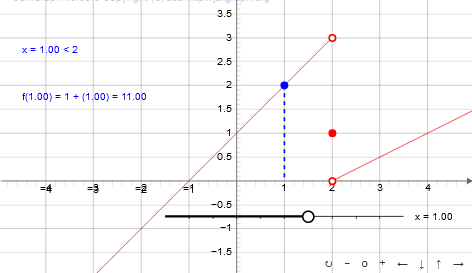
\includegraphics[width=\linewidth]{external/jsxgraph-limitnumerically.png}
\end{sbspanel}%
\begin{sbspanel}{0.21}%

\includegraphics[width=\linewidth]{generated/qrcode/sec-ComputingLimitsNumerically-4.png}
\href{http://webwork.bridgew.edu/oer/functions_at_work/sec-ComputingLimitsNumerically-4.html}{Standalone}%
\par
\href{http://webwork.bridgew.edu/oer/functions_at_work/sec-ComputingLimitsNumerically-4-if.html}{Embed}%
\end{sbspanel}%
\end{sidebyside}%
\par
We can use the equation%
\begin{exploration}{Exploration}{}{sec-ComputingLimitsNumerically-6}%
Suppose that the cost of producing \(x\) barrels of oil is given by%
\begin{equation*}
C(x) = 
\begin{cases}
50 + 5x & \text{ if } x\lt 10 \\ 
125     & \text{ if } x = 10 \\ 
90 + 6x & \text{ if } x\gt 10 \\ 
\end{cases}
\end{equation*}
%
\begin{enumerate}[font=\bfseries,label=(\alph*),ref=\alph*]%
\item{}Compute \(\displaystyle \lim_{x\rightarrow 10^+} C(x)\)%
\par\smallskip%
\noindent\textbf{\blocktitlefont Solution}.\hypertarget{sec-ComputingLimitsNumerically-6-2-2}{}\quad{}Think about some \(x\) values you would pass through when approaching \(10\) from the right. For example, you would pass through \(x=11,\ x=10.5,\ x=10.1,\ x=10.01\) and so on. Compute the height at each of the \(x\) values we listed above. \begin{center}%
{\tabularfont%
\begin{tabular}{lBl}
\(x\)&\(C(x)\)\tabularnewline\hrulemedium
\(11\)&\(C(11) =  90 + 6(11) = 156  \)\tabularnewline\hrulemedium
\(10.5\)&\(C(10.5) = 90 + 6(10.5) = 153  \)\tabularnewline\hrulemedium
\(10.1\)&\(C(10.1) =  90 + 6(10.1) =150.6  \)\tabularnewline\hrulemedium
\(10.01\)&\(C(10.01) = 90 + 6(10.01) =150.06   \)
\end{tabular}
}%
\end{center}%
 As you move from the top row of the table to the bottom row of the table, the \(x\) values get closer and closer to \(a=10\), always from the right.%
\par
And as these \(x\) values approach 10, we see that the heights \(C(x)\) get closer and closer to 150.  That means%
\begin{equation*}
\lim_{x\rightarrow 10^+} C(x) = 150
\end{equation*}
%
\item{}Compute \(\displaystyle \lim_{x\rightarrow 10^-} C(x)\)%
\par\smallskip%
\noindent\textbf{\blocktitlefont Solution}.\hypertarget{sec-ComputingLimitsNumerically-6-3-2}{}\quad{}Think about some \(x\) values you would pass through when approaching \(10\) from the left. For example, you would pass through \(x=9,\ x=9.5,\ x=9.9,\ x=9.99\) and so on. Compute the height at each of the \(x\) values we listed above. \begin{center}%
{\tabularfont%
\begin{tabular}{lBl}
\(x\)&\(C(x)\)\tabularnewline\hrulemedium
\(9\)&\(C(9) =  90 + 6(11) = 95  \)\tabularnewline\hrulemedium
\(9.5\)&\(C(9.5) = 90 + 6(10.5) = 97.5  \)\tabularnewline\hrulemedium
\(9.9\)&\(C(9.9) =  90 + 6(10.1) =99.5  \)\tabularnewline\hrulemedium
\(9.99\)&\(C(9.99) = 90 + 6(10.01) = 99.95\)
\end{tabular}
}%
\end{center}%
 As you move from the top row of the table to the bottom row of the table, the \(x\) values get closer and closer to \(a=10\), always from the left.%
\par
And as these \(x\) values approach 10, we see that the heights \(C(x)\) get closer and closer to 100.  That means%
\begin{equation*}
\lim_{x\rightarrow 10^-} C(x) = 100
\end{equation*}
%
\item{}Is \(C(x)\) continuous at \(x=10\)?  If not, classify the type of discontinuity.%
\par\smallskip%
\noindent\textbf{\blocktitlefont Solution}.\hypertarget{sec-ComputingLimitsNumerically-6-4-2}{}\quad{}We have seen above that the left and right hand limits exist, but do not equal eachother.  In other words, we have seen that%
\begin{equation*}
\lim_{x\rightarrow 10} C(x) DNE\text{.}
\end{equation*}
It follows that the function is not continuous at \(a=10\).%
\par
Because the directed limits exist and equal finite numbers, this is a \emph{jump discontinuity}.%
\end{enumerate}%
\end{exploration}%
\begin{inlineexercise}{Checkpoint}{}{sec-ComputingLimitsNumerically-7}%
Let \(A(x) = \dfrac{10+4x}{x}\). Find \(\displaystyle\lim_{x\rightarrow 0^+} A(x)\).%
\par\smallskip%
\noindent\textbf{\blocktitlefont Solution}.\hypertarget{sec-ComputingLimitsNumerically-7-2}{}\quad{}Think about some \(x\) values you would pass through when approaching \(0\) from the right. For example, you would pass through \(x=1,\ x=0.5,\ x=0.1,\ x=0.01\) and so on. Compute the height at each of the \(x\) values we listed above. \begin{center}%
{\tabularfont%
\begin{tabular}{lBl}
\(x\)&\(f(x)\)\tabularnewline\hrulemedium
\(1\)&\(f(1) = \dfrac{10+4(1)}{1} = 14  \)\tabularnewline\hrulemedium
\(0.5\)&\(f(0.5) = \dfrac{10+4(0.5)}{0.5} = 24  \)\tabularnewline\hrulemedium
\(0.1\)&\(f(0.1) = \dfrac{10+4(0.1)}{0.1} = 104 \)\tabularnewline\hrulemedium
\(0.01\)&\(f(0.01) = \dfrac{10+4(0.01)}{0.01} = 1,004  \)\tabularnewline[0pt]
\(0.001\)&\(f(0.001) = \dfrac{10+4(0.001)}{0.001} = 10,004  \)
\end{tabular}
}%
\end{center}%
 As you move from the top row of the table to the bottom row of the table, the \(x\) values get closer and closer to \(a=0\), always from the right.%
\par
And as these \(x\) values approach 0, we see that the heights \(f(x)\) are getting bigger and bigger, without bound.  That means%
\begin{equation*}
\lim_{x\rightarrow 10^+} f(x) = \infty
\end{equation*}
%
\begin{sidebyside}{2}{0.075}{0.075}{0.17}%
\begin{sbspanel}{0.47}%
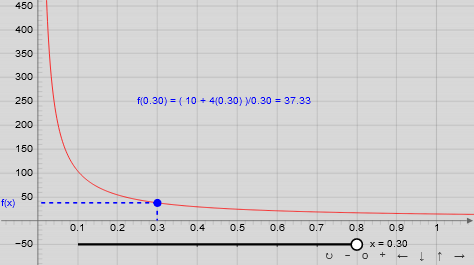
\includegraphics[width=\linewidth]{external/jsxgraph-inflimit.png}
\end{sbspanel}%
\begin{sbspanel}{0.21}%

\includegraphics[width=\linewidth]{generated/qrcode/sec-ComputingLimitsNumerically-7-2-3.png}
\href{http://webwork.bridgew.edu/oer/functions_at_work/sec-ComputingLimitsNumerically-7-2-3.html}{Standalone}%
\par
\href{http://webwork.bridgew.edu/oer/functions_at_work/sec-ComputingLimitsNumerically-7-2-3-if.html}{Embed}%
\end{sbspanel}%
\end{sidebyside}%
\end{inlineexercise}%
\end{sectionptx}
\end{chapterptx}
 %
%
\typeout{************************************************}
\typeout{Chapter 8 Average Rates of Change}
\typeout{************************************************}
%
\begin{chapterptx}{Chapter}{Average Rates of Change}{}{Average Rates of Change}{}{}{ch_totalschanges}
\renewcommand*{\chaptername}{Chapter}
\begin{introduction}{}%
The concepts contained in \hyperref[ch_limits]{Chapter~{\xreffont\ref{ch_limits}}\textendash{}{\xreffont\ref{ch_tangentsecant}}} are all connected in important, but sometimes tricky to follow ways.  As you go through this section, you may find it helpful to refer to the diagram below to see how the concepts we have seen so far are related.%
\begin{image}{0}{1}{0}{}%
\resizebox{\linewidth}{!}{%
     \begin{tikzpicture}
\node[inner sep=0pt] (O) at (0,0) {};
\node (limg) at (3,1.5) {graphical limits};
\node (limn) at (7,1.5) {numerical limits};
\node (change) at (3,0) {change $\Delta C$};
\node (aroc) at (7,0) {average change $\frac{\Delta C}{\Delta x}$} ;
%\node (slopeg) at (3,-1.5) {slopes from tangents};
%\node (slopesec) at (8,-1.5) {approx (secant) slope $\frac{\Delta C}{\Delta x}$};
\node (velocity) at (12,0) {\begin{minipage}{1.25in}\centering velocity and IROC \\ $\lim_{\Delta x\rightarrow 0}\frac{\Delta y}{\Delta x}$\end{minipage}} ;
%\node (slopen) at (14,-1.5) {\begin{minipage}{1.25in}\centering  slope numerically \\ $\lim_{h\rightarrow 0}\frac{f(a+h) - f(a)}{h}$\end{minipage}};

\draw[fill] (O) circle (2pt);
\draw[-latex] (O) -- (limg);
\draw[-latex] (limg) -- (limn);
\draw[-latex] (limn) -- (velocity);
\draw (O) -- (change) ;
\draw[-latex] (change) -- (aroc) ;
\draw[-latex] (aroc) -- (velocity) ; 
     \end{tikzpicture}
}%
\end{image}%
\end{introduction}%
%
%
\typeout{************************************************}
\typeout{Section 8.1 Average Rates of Change}
\typeout{************************************************}
%
\begin{sectionptx}{Section}{Average Rates of Change}{}{Average Rates of Change}{}{}{sec-AROC}
Let \(y\) be any function of \(x\). That means that any change of input \(\Delta x\) produces a change in the output \(\Delta y\). If we \emph{average} the change in outputs \(\Delta y\) over the inputs \(\Delta x\), we get the \terminology{average change} \(\dfrac{\Delta y}{\Delta x}\).%
\par
For reasons we will see in a future section, we will use the terms \terminology{average change} and \terminology{average rate of change} interchangeably.%
\begin{definition}{Definition}{}{def-averagerate}%
Given a curve \(y=f(x)\) and two input values \(x_1\) and \(x_2\)%
\begin{itemize}[label=\textbullet]
\item{}The \terminology{change in input} that results from moving from \(x_1\) to \(x_2\) is \(\Delta x = x_2-x_1\)%
\item{}The resulting \terminology{change in output} that results from moving from \(x_1\) to \(x_2\) is%
\begin{equation*}
\Delta y = y_2-y_1 = f(x_2) - f(x_1)
\end{equation*}
where \(y_1 = f(x_1)\) and \(y_2=f(x_2)\).%
\item{}The \terminology{average rate of change of \(y\)} as a result of changing the inputs from \(x_1\) to \(x_2\) is%
\begin{equation*}
\dfrac{\Delta y}{\Delta x} = \dfrac{y_2-y_1}{x_2-x_1} = \dfrac{f(x_2) - f(x_1)}{x_2-x_1}
\end{equation*}
%
\end{itemize}
%
\end{definition}
\begin{inlineexercise}{Checkpoint}{}{sec-AROC-5}%
Recall that the total cost function \(C(x)\) is a function of the total number of items \(x\) to be produced. Suppose that increasing your production by 100 items will increase the total cost by \textdollar{}2000. Find the \emph{average} (aka \emph{average rate of}) change in the cost.%
\par\smallskip%
\noindent\textbf{\blocktitlefont Solution}.\hypertarget{sec-AROC-5-2}{}\quad{}We are told that a change of input \(\Delta x = 100\) will result in an increase in total cost of \(\Delta C = 2000\). To find the \emph{average} change, divide that \textdollar{}2000 evenly across the 100 additional items%
\begin{equation*}
\dfrac{\Delta C}{\Delta x} = \dfrac{2000}{100} = 20
\end{equation*}
On average, each of the 100 additional items will increase the total cost by \textdollar{}20.%
\end{inlineexercise}%
Average rates are common throughout economics and daily life. When the number of items is large (in the context of macroeconomics), limits show up and calculus begins. But before we get there, we will first explore a number of examples that emphasize the connection between \emph{totals}, \emph{changes} and \emph{averages\slash{}rates}.%
\begin{exploration}{Exploration}{}{sec-AROC-7}%
A total (cumulative) cost function is defined by \(C(x) = 0.1 x^2 + 50 x + 1000 \) in dollars as a function of the total number of items \(x\) to be produced.%
\begin{enumerate}[font=\bfseries,label=(\alph*),ref=\alph*]%
\item{}Last year, you made 100 items. This year, you are considering increasing your production to 150 items. Find the \emph{change} in cost and the \emph{average rate of change} in the cost that would result from this change.%
\par\smallskip%
\noindent\textbf{\blocktitlefont Solution}.\hypertarget{sec-AROC-7-2-2}{}\quad{}From the information given in the problem, we can compute the total cost of producing 100 items is%
\begin{equation*}
C_1 = C(100) = \$ 7, 000
\end{equation*}
and that the total cost of producing 150 items would be%
\begin{equation*}
C_2 = C(150) = \$ 10, 750
\end{equation*}
The change in cost between these quantities is%
\begin{equation*}
\Delta C = C(150) - C(100) = 10,750 - 7,000 = \$ 3,750
\end{equation*}
This change is a result of changing the quantity by%
\begin{equation*}
\Delta x = 150 - 100 = 50 \text{ items}
\end{equation*}
. Dividing the total cost \(\Delta C\) evenly among the \(\Delta x\) items results in an \emph{average} cost per item of%
\begin{equation*}
\dfrac{\Delta C}{\Delta x} = \dfrac{3,750}{50} = 75 \frac{\$}{\text{item}}
\end{equation*}
%
\par
There were a lot of parts of this calculation.  You can either use a the definition \(\dfrac{\Delta C}{\Delta x} = \dfrac{C(x_2) - C(x_1)}{x_2 - x_1} \) which is a single formula that combines all of these steps, or you can organize the different parts separately using the table below. This is called an Average Rate of Change table, often abbreviated AROC. \begin{center}%
{\tabularfont%
\begin{tabular}{lBlBlBlBlBlBl}
\(x_1\)&\(x_2\)&\(\Delta x\)&\(y_1\)&\(y_2\)&\(\Delta y\)&\(\Delta y/\Delta x\)\tabularnewline\hrulemedium
\(100\)&\(150\)&\(50\)&\(7000\)&\(10750\)&\(3750\)&\(75\)
\end{tabular}
}%
\end{center}%
%
\item\label{task_costfunctionwithdecreasingquantity}Use the cost function above to find the average change in cost between 100 and 125 items, between 100 and 110 items, and between 100 and 101 items.%
\par\smallskip%
\noindent\textbf{\blocktitlefont Solution}.\hypertarget{task_costfunctionwithdecreasingquantity-2}{}\quad{}\begin{center}%
{\tabularfont%
\begin{tabular}{lBlBlBlBlBlBl}
\(x_1\)&\(x_2\)&\(\Delta x\)&\(y_1\)&\(y_2\)&\(\Delta y\)&\(\Delta y/\Delta x\)\tabularnewline\hrulemedium
\(100\)&\(125\)&\(\color{red} 	125 - 100 = 25\)&\(\color{blue} C(100) = 7000\)&\(\color{blue} C(125) = 8812.5\)&\(\color{blue} C(125) - C(100) \color{green} = 8812.5 - 7000 = 1812.5 \)&\(\dfrac{\color{green} 1812.5}{\color{red} 25} = 72.50  \)\tabularnewline\hrulemedium
\(100\)&\(110\)&\(\color{red} 	110 - 100 = 10\)&\(\color{blue} C(100) = 7000\)&\(\color{blue} C(110) = 7710 \)&\(\color{blue} C(110) - C(100) \color{green} = 7710 - 7000 = 710 \)&\(\dfrac{\color{green} 710}{\color{red} 10} = 71.00  \)\tabularnewline\hrulemedium
\(100\)&\(101\)&\(\color{red} 	101 - 100 = 1\)&\(\color{blue} C(100) = 7000\)&\(\color{blue} C(101) = 7070.1\)&\(\color{blue} C(101) - C(100) \color{green} =  7070.1 - 7000 = 70.1\)&\(\dfrac{\color{green} 70.1}{\color{red} 1} =  70.10 \)
\end{tabular}
}%
\end{center}%
%
\item{}Suppose that last year you produced 100 items, and that you are planning to increasing production by 5 items this year. Find the average rate of change in cost that results from this change.%
\par\smallskip%
\noindent\textbf{\blocktitlefont Solution}.\hypertarget{sec-AROC-7-4-2}{}\quad{}We are given the starting quantity \(x_1 = 5\) and the change in quantity \(\Delta x = 5\).  Using this, we can reason backward to get the ending quantity \(x_2 = 105\). We can use the AROC equation%
\begin{equation*}
\dfrac{\Delta C}{\Delta x} = \dfrac{C(105) - C(100)}{105-100} = \dfrac{7352.5 - 7000}{5} = 70.5
\end{equation*}
or create an AROC table \begin{center}%
{\tabularfont%
\begin{tabular}{lBlBlBlBlBlBl}
\(x_1\)&\(x_2\)&\(\Delta x\)&\(y_1\)&\(y_2\)&\(\Delta y\)&\(\Delta y/\Delta x\)\tabularnewline\hrulemedium
\(100\)&\(105\)&\(\color{red} 	105 - 100 = 5\)&\(\color{blue} C(100) = 7000\)&\(\color{blue} C(105) = 7352.5\)&\(\color{blue} C(105) - C(100) \color{green} =  7352.5 - 7000 = 352.5\)&\(\dfrac{\color{green} 362.5}{\color{red} 5} =  70.50 \)
\end{tabular}
}%
\end{center}%
 The 5 additional items will increase the \emph{total cost} by an average of 70.50 \emph{dollars per item}.%
\end{enumerate}%
\end{exploration}%
\end{sectionptx}
%
%
\typeout{************************************************}
\typeout{Section 8.2 Graphs of Rates, Changes, and Totals}
\typeout{************************************************}
%
\begin{sectionptx}{Section}{Graphs of Rates, Changes, and Totals}{}{Graphs of Rates, Changes, and Totals}{}{}{sec_graphsofrateschangesandtotals}
\begin{insight}{Application}{Understanding and Applying "Average Rates of Change".}{insight-applyingAROC}%
We've spent a lot of time thinking about ``total'' and ``change'' graphs. In each of those examples, we knew the value of the total for each natural number \(1,2,3,\dots\)%
\par
But what happens if we only have information about \emph{a few} values of \(x\). For example, in the graph on the right, we only know the total value on day 0, 5, 10, etc.%
\par
What should we do if we want to know the change between day 0 and 1? We can't know that number for certain, but we \emph{can} try to compute the \emph{average} change.%
\par
Since the value went up 2 units over 5 days, if we divide that change evenly over the 5 days we get the \terminology{Average Rate Of Change}%
\begin{equation*}
\text{(AROC)} = \dfrac{\Delta y}{\Delta x} = \dfrac{y_2 - y_1}{x_2 - x_1} = \dfrac{4-2}{5-0} = \dfrac{2}{5} = 0.4
\end{equation*}
%
\begin{image}{0.3}{0.4}{0.3}{}%
\resizebox{\linewidth}{!}{%
\def \tikzhistogram (#1,#2){\draw[fill=blue,opacity=0.3] ({#1+((\xtwo-\xmin)/5)},#2) rectangle ({#1-((\xtwo-\xmin)/5)},0); \draw[draw,thick] ({#1+((\xtwo-\xmin)/5)},#2) rectangle ({#1-((\xtwo-\xmin)/5)},0); \node[draw,fill=blue, circle,inner sep=2.5pt] at (#1,#2) {};}
\def \xmin {0}
\def \xmax {30}
\def \xtwo {5}
\def \xunits { } 
\def \yunits { }
\def \dyunits { }
\def \yscale {1}
\def \xscale {0.1}
%% Information about the total (y) graph
\def \ymin {0}								%% First height to be be drawn with dashed lines
\def \ysecondmajoraxis {1}		%% Second height to be be drawn with dashed lines
\def \yfirstminoraxis  {0.5}	%% First line to be drawn with dotted lines
\def \ysecondminoraxis {1.5}	%% Second lin eto be drawn with dotted lines
\def \ymax {5}
%% Information about the change (\Delta y) graph
\def \dymin {-2}
\def \dysecondmajoraxis {-1}
\def \dyfirstminoraxis  {-1.5}
\def \dysecondminoraxis {-0.5}
\def \dymax {2.5}

\begin{tikzpicture}[xscale=\xscale,yscale=\yscale]
\def \yscale {1}
	%% Graph of Total %%
	%\draw ({\xmin-1},{\ymin-1}) rectangle ({\xmax+1.5},{\ymax+1.25});
	%\node at ({(\xmin+\xmax)/2},{\ymin-1.75}) {Graph of Total \ $y$};
	%\node at ({(\xmin+\xmax)/2},{\ymin-1.75}) {$\phantom{\dfrac{\Delta y}{\Delta x}}$};
	%
	%% Draw horizontal lines at major and minor y-values
	\foreach \i in {\ymin,\ysecondmajoraxis,...,\ymax}
		\draw[major gridlines] (\xmin,\i)--({\xmax+1},\i);
	\foreach \i in {\yfirstminoraxis,\ysecondminoraxis,...,\ymax}
		\draw[minor gridlines] (\xmin,\i)--({\xmax+1},\i);
	%
	%% Draw and label x and y axes
	\draw[axes,-latex] ({\xmin},0) -- ({\xmax+1},0) node [below] {\xunits};
	\draw[axes,-latex] (0,{\ymin}) -- (0,{\ymax+0.5}) node [above right] {\yunits};
	\foreach \i in {\xmin,\xtwo,...,\xmax}
		\node[below,fill=white,yshift=-2pt] at (\i, 0) {\small $\i$};
	\foreach \i in {\ymin,...,\ymax}
		\node[left,fill=white,xshift=-2pt] at (0,\i) {\small $\i$};
	
	\foreach \i in {\xmin,\xtwo,...,\xmax}
		\draw[vertical gridlines] (\i, {\ymin}) -- (\i, {\ymax+0.25});
	
	%\draw[draw=black,thick,fill=blue,opacity=0.75] (1,4) rectangle ({1-1},0);
		

	\tikzhistogram(0,2);
	\tikzhistogram(5,4);
	\tikzhistogram(10,3);
	\tikzhistogram(15,2.5);
	\tikzhistogram(20,3.5);
	\tikzhistogram(25,3);
	\tikzhistogram(30,2);
	
	% standard dimension:
	%		\draw [dimen] (1,0) -- (1,1.75) node {$f(x)$};
	% short dimension:
	%   \draw [dimen] (0,-.5) -- (0.4,-.5) node[below=1mm,midway] {$\Delta x$};
	\draw[dimen,red] (-15,2) -- (-15,4) node [left=1mm,midway] {$\Delta y$} ;
	\draw[dimen,red] (0,-1.25) -- (5,-1.25) node [below=1mm,midway] {$\phantom{\scriptstyle[0,5]}\Delta x\ _{[0,5]}$} ;
	\node at (-2,2) [left,red] {$y_1=$};	
	\node at (-2,4) [left,red] {$y_2=$};	
	\node at (0,-0.5) [below,red] {$x_1$};	
	\node at (5,-0.5) [below,red] {$x_2$};	


\end{tikzpicture}
}%
\end{image}%
Summarizing this in a table, we get the row in an Average Rate Of Change (AROC) table:%
\begin{center}%
{\tabularfont%
\begin{tabular}{lBlBlBlBlBlBl}
\(x_1\)&\(x_2\)&\(\Delta x\)&\(y_1\)&\(y_2\)&\(\Delta y\)&\(\Delta y/\Delta x\)\tabularnewline\hrulemedium
\(0\)&\(5\)&\(\color{red} 	5 - 0 = 5\)&\(\color{blue} C(0) = 2\)&\(\color{blue} C(5) = 4\)&\(\color{blue} C(0) - C(5) \color{green} = 2\)&\(\dfrac{\color{green} 2}{\color{red} 5} = 0.4\)
\end{tabular}
}%
\end{center}%
\end{insight}
\begin{exploration}{Exploration}{}{sec_graphsofrateschangesandtotals-3}%
Suppose, as in \hyperref[insight-applyingAROC]{Application~{\xreffont\ref{insight-applyingAROC}}}, that a total cost function is given by the histogram below%
\begin{image}{0.3}{0.4}{0.3}{}%
\resizebox{\linewidth}{!}{%
\def \tikzhistogram (#1,#2){\draw[fill=blue,opacity=0.3] ({#1+((\xtwo-\xmin)/5)},#2) rectangle ({#1-((\xtwo-\xmin)/5)},0); \draw[draw,thick] ({#1+((\xtwo-\xmin)/5)},#2) rectangle ({#1-((\xtwo-\xmin)/5)},0); \node[draw,fill=blue, circle,inner sep=2.5pt] at (#1,#2) {};}
\def \xmin {0}
\def \xmax {30}
\def \xtwo {5}
\def \xunits { } 
\def \yunits { }
\def \dyunits { }
\def \yscale {1}
\def \xscale {0.1}
%% Information about the total (y) graph
\def \ymin {0}								%% First height to be be drawn with dashed lines
\def \ysecondmajoraxis {1}		%% Second height to be be drawn with dashed lines
\def \yfirstminoraxis  {0.5}	%% First line to be drawn with dotted lines
\def \ysecondminoraxis {1.5}	%% Second lin eto be drawn with dotted lines
\def \ymax {5}
%% Information about the change (\Delta y) graph
\def \dymin {-2}
\def \dysecondmajoraxis {-1}
\def \dyfirstminoraxis  {-1.5}
\def \dysecondminoraxis {-0.5}
\def \dymax {2.5}

\begin{tikzpicture}[xscale=\xscale,yscale=\yscale]
\def \yscale {1}
	%% Graph of Total %%
	%\draw ({\xmin-1},{\ymin-1}) rectangle ({\xmax+1.5},{\ymax+1.25});
	%\node at ({(\xmin+\xmax)/2},{\ymin-1.75}) {Graph of Total \ $y$};
	%\node at ({(\xmin+\xmax)/2},{\ymin-1.75}) {$\phantom{\dfrac{\Delta y}{\Delta x}}$};
	%
	%% Draw horizontal lines at major and minor y-values
	\foreach \i in {\ymin,\ysecondmajoraxis,...,\ymax}
		\draw[major gridlines] (\xmin,\i)--({\xmax+1},\i);
	\foreach \i in {\yfirstminoraxis,\ysecondminoraxis,...,\ymax}
		\draw[minor gridlines] (\xmin,\i)--({\xmax+1},\i);
	%
	%% Draw and label x and y axes
	\draw[axes,-latex] ({\xmin},0) -- ({\xmax+1},0) node [below] {\xunits};
	\draw[axes,-latex] (0,{\ymin}) -- (0,{\ymax+0.5}) node [above right] {\yunits};
	\foreach \i in {\xmin,\xtwo,...,\xmax}
		\node[below,fill=white,yshift=-2pt] at (\i, 0) {\small $\i$};
	\foreach \i in {\ymin,...,\ymax}
		\node[left,fill=white,xshift=-2pt] at (0,\i) {\small $\i$};
	
	\foreach \i in {\xmin,\xtwo,...,\xmax}
		\draw[vertical gridlines] (\i, {\ymin}) -- (\i, {\ymax+0.25});
	
	%\draw[draw=black,thick,fill=blue,opacity=0.75] (1,4) rectangle ({1-1},0);
		

	\tikzhistogram(0,2);
	\tikzhistogram(5,4);
	\tikzhistogram(10,3);
	\tikzhistogram(15,2.5);
	\tikzhistogram(20,3.5);
	\tikzhistogram(25,3);
	\tikzhistogram(30,2);
	
	% standard dimension:
	%		\draw [dimen] (1,0) -- (1,1.75) node {$f(x)$};
	% short dimension:
	%   \draw [dimen] (0,-.5) -- (0.4,-.5) node[below=1mm,midway] {$\Delta x$};
\end{tikzpicture}
}%
\end{image}%
\begin{enumerate}[font=\bfseries,label=(\alph*),ref=\alph*]%
\item{}Fill in the following AROC table \begin{center}%
{\tabularfont%
\begin{tabular}{lBlBlBlBlBlBl}
\(x_1\)&\(x_2\)&\(\Delta x\)&\(y_1\)&\(y_2\)&\(\Delta y\)&\(\Delta y/\Delta x\)\tabularnewline\hrulemedium
\(0\)&\(5\)&\(\)&\(\)&\(\)&\(\)&\(\)\tabularnewline\hrulemedium
\(5\)&\(10\)&\(\)&\(\)&\(\)&\(\)&\(\)\tabularnewline\hrulemedium
\(10\)&\(15\)&\(\)&\(\)&\(\)&\(\)&\(\)\tabularnewline\hrulemedium
\(15\)&\(20\)&\(\)&\(\)&\(\)&\(\)&\(\)
\end{tabular}
}%
\end{center}%
%
\par\smallskip%
\noindent\textbf{\blocktitlefont Solution}.\hypertarget{sec_graphsofrateschangesandtotals-3-2-2}{}\quad{}\begin{center}%
{\tabularfont%
\begin{tabular}{lBlBlBlBlBlBl}
\(x_1\)&\(x_2\)&\(\Delta x\)&\(y_1\)&\(y_2\)&\(\Delta y\)&\(\Delta y/\Delta x\)\tabularnewline\hrulemedium
\(0\)&\(5\)&\(\color{red} 5-0 = 5\)&\(\color{blue} 2\)&\(\color{blue} 4\)&\(\color{blue} 4-2 \color{green} = 2\)&\(\dfrac{\color{green} 2}{\color{red} 5} = 0.4\)\tabularnewline\hrulemedium
\(5\)&\(10\)&\(\color{red} 10-5 = 5\)&\(\color{blue} 4\)&\(\color{blue} 3\)&\(\color{blue} 3-4 \color{green} = -1\)&\(\dfrac{\color{green} -1}{\color{red} 5}=-0.2\)\tabularnewline\hrulemedium
\(10\)&\(15\)&\(\color{red} 15-10=5\)&\(\color{blue} 3\)&\(\color{blue} 2.5\)&\(\color{blue} 2.5-3 \color{green} = -0.5\)&\(\dfrac{\color{green} -0.5}{\color{red} 5}=-0.1\)\tabularnewline\hrulemedium
\(15\)&\(20\)&\(\color{red} 20-15 = 5\)&\(\color{blue} 2.5\)&\(\color{blue} 3.5\)&\(\color{blue} 3.5-2.5 \color{green} = 1\)&\(\dfrac{\color{green} 1}{\color{red} 5}=0.2\)
\end{tabular}
}%
\end{center}%
%
\item{}Use your AROC table to fill in the graphs of the change \(\Delta y\) and of the rate \(\dfrac{\Delta y}{\Delta x}\) in the graph below.%
\begin{image}{0.275}{0.45}{0.275}{}%
\resizebox{\linewidth}{!}{%
%%%% EXAMPLE 1 %%%%
\def \tikzhistogram (#1,#2){\draw[fill=blue,opacity=0.3] ({#1+((\xtwo-\xmin)/5)},#2) rectangle ({#1-((\xtwo-\xmin)/5)},0); \draw[draw,thick] ({#1+((\xtwo-\xmin)/5)},#2) rectangle ({#1-((\xtwo-\xmin)/5)},0); \node[draw,fill=blue, circle,inner sep=2.5pt] at (#1,#2) {};}
%\def \tikzhistogram (#1,#2){\draw[fill=blue,opacity=0.3] ({#1+0.25},#2) rectangle ({#1-0.25},0); \draw[draw,thick] ({#1+0.25},#2) rectangle ({#1-0.25},0); \node[draw,fill=blue, circle,inner sep=2.5pt] at (#1,#2) {};}
\def \xmin {0}
\def \xmax {22}
\def \xtwo {5}
\def \xunits { } 
\def \yunits { }
\def \dyunits { }
\def \yscale {2}
\def \xscale {.2*0.75}
%% Information about the total (y) graph
\def \ymin {0}								%% First height to be be drawn with dashed lines
\def \ysecondmajoraxis {1}		%% Second height to be be drawn with dashed lines
\def \yfirstminoraxis  {0.5}	%% First line to be drawn with dotted lines
\def \ysecondminoraxis {1.5}	%% Second lin eto be drawn with dotted lines
\def \ymax {4}
%% Information about the change (\Delta y) graph
\def \dymin {-2}
\def \dysecondmajoraxis {-1}
\def \dyfirstminoraxis  {-1.5}
\def \dysecondminoraxis {-0.5}
\def \dymax {2}

\begin{tikzpicture}[xscale=\xscale,yscale=\yscale]
	%% Graph of Total %%
	%\draw ({\xmin-1},{\ymin-1}) rectangle ({\xmax+1.5},{\ymax+1.25});
	\node at ({(\xmin+\xmax)/2},{\ymin-0.75}) {Graph 1: of Total \ $y$};
	\node at ({(\xmin+\xmax)/2},{\ymin-0.75}) {$\phantom{\dfrac{\Delta y}{\Delta x}}$};
	%
	%% Draw horizontal lines at major and minor y-values
	\foreach \i in {\ymin,\ysecondmajoraxis,...,\ymax}
		\draw[major gridlines] (\xmin,\i)--({\xmax+1},\i);
	\foreach \i in {\yfirstminoraxis,\ysecondminoraxis,...,\ymax}
		\draw[minor gridlines] (\xmin,\i)--({\xmax+1},\i);
	%
	%% Draw and label x and y axes
	\draw[axes,-latex] ({\xmin},0) -- ({\xmax+1},0) node [below] {\xunits};
	\draw[axes,-latex] (0,{\ymin}) -- (0,{\ymax+0.5}) node [above right] {\yunits};
	\foreach \i in {\xmin,\xtwo,...,\xmax}
		\node[below,fill=white,yshift=-2pt] at (\i, 0) {\small $\i$};
	\foreach \i in {\ymin,...,\ymax}
		\node[left,fill=white,xshift=-2pt] at (0,\i) {\small $\i$};
	
	\foreach \i in {\xmin,\xtwo,...,\xmax}
		\draw[vertical gridlines] (\i, {\ymin}) -- (\i, {\ymax+0.25});
	
	%\draw[draw=black,thick,fill=blue,opacity=0.75] (1,4) rectangle ({1-1},0);
		
	\tikzhistogram(0,2);
	\tikzhistogram(5,4);
	\tikzhistogram(10,3);
	\tikzhistogram(15,2.5);
	\tikzhistogram(20,3.5);
	%\tikzhistogram(25,3);
	%\tikzhistogram(30,2);
	
\end{tikzpicture}
%
\ 
%
\begin{tikzpicture}[xscale=\xscale,yscale=\yscale]
	%% Graph of Change %%
	%\draw ({\xmin-1.5},{\dymin-1}) rectangle ({\xmax+1.5},{\dymax+1.25});
	\node at ({(\xmin+\xmax)/2},{\dymin-0.75}) {Graph 2: Change \ $\Delta y$};
	\node at ({(\xmin+\xmax)/2},{\dymin-0.75}) {$\phantom{\dfrac{\Delta y}{\Delta x}}$};
	%	%
	%% Draw horizontal lines at major and minor y-values
	\foreach \i in {\dymin,\dysecondmajoraxis,...,\dymax}
		\draw[major gridlines] (\xmin,\i)--({\xmax+1},\i);
	\foreach \i in {\dyfirstminoraxis,\dysecondminoraxis,...,\dymax}
		\draw[minor gridlines] (\xmin,\i)--({\xmax+1},\i);
	%
	%% Draw and label x and y axes
	\draw[axes,-latex] ({\xmin},0) -- ({\xmax+1},0) node [below] {\xunits};
	\draw[axes,latex-latex] (0,{\dymin}) -- (0,{\dymax})  node[above right]{\dyunits};
	\foreach \i in {\xmin,\xtwo,...,\xmax}
		\node[below,fill=white,yshift=-6pt] at (\i, \dymin) {\small $\i$};
	\foreach \i in {\dymin,...,\dymax}
		\node[left,fill=white,xshift=-2pt] at (0,\i) {\small $\i$};

	\node[left] at (0,0.5) {\scriptsize 0.5};
	\node[left] at (0,-0.5) {\scriptsize -0.5};
	
	\foreach \i in {\xmin,\xtwo,...,\xmax}
		\draw[vertical gridlines] (\i, {\dymin-0.25}) -- (\i, {\dymax+0.25});
	
	
	%\tikzhistogram(0,0);
	\tikzhistogram(5,2);
	%\tikzhistogram(10,-1);
	%\tikzhistogram(15,-.5);
	%\tikzhistogram(20,1);
	%\tikzhistogram(25,-.5);
	%\tikzhistogram(30,-1);
	
\end{tikzpicture}
%
\ 
%
\begin{tikzpicture}[xscale=\xscale,yscale=\yscale]
	%% Graph of Change %%
	%\draw ({\xmin-1.5},{\dymin-1}) rectangle ({\xmax+1.5},{\dymax+1.25});
	\node at ({(\xmin+\xmax)/2},{\dymin-0.75}) {Graph 3: Rate \ $\dfrac{\Delta y}{\Delta x}$};
	%
	%% Draw horizontal lines at major and minor y-values
	\foreach \i in {\dymin,\dysecondmajoraxis,...,\dymax}
		\draw[major gridlines,thick] (\xmin,\i)--({\xmax+1},\i);
	
	\foreach \i in {-1.8,-1.6,-1.4,-1.2,-0.8,-0.6,-0.4,-0.2,1.8,1.6,1.4,1.2,0.8,0.6,0.4,0.2}
		\draw[very thin] (\xmin,\i)--({\xmax+1},\i);
	%
	%% Draw and label x and y axes
	\draw[axes,-latex] ({\xmin},0) -- ({\xmax+1},0) node [below] {\xunits};
	\draw[axes,latex-latex] (0,{\dymin}) -- (0,{\dymax})  node[above right]{\dyunits};
	
	\foreach \i in {\xmin,\xtwo,...,\xmax}
		\node[below,fill=white,yshift=-6pt] at (\i, \dymin) {\small $\i$};
	
	\foreach \i in {\dymin,\dysecondmajoraxis,...,\dymax}
		\node[left,fill=white,xshift=-2pt] at (0,\i) {\small $\i$};

	\foreach \i in {0.2,0.4,0.6,0.8,-0.2,-0.4,-0.6,-0.8}
		\node[left] at (0,\i) {\scriptsize \i};
	
	\foreach \i in {\xmin,\xtwo,...,\xmax}
		\draw[vertical gridlines] (\i, {\dymin-0.25}) -- (\i, {\dymax+0.25});
	
	
	%\tikzhistogram(0,0/5);
	\tikzhistogram(5,2/5);
	%\tikzhistogram(10,-1/5);
	%\tikzhistogram(15,-.5/5);
	%\tikzhistogram(20,1/5);
	%\tikzhistogram(25,-.5/5);
	%\tikzhistogram(30,-1/5);
	
\end{tikzpicture}
%%%% END EXAMPLE 1 %%%%
}%
\end{image}%
\par\smallskip%
\noindent\textbf{\blocktitlefont Solution}.\hypertarget{sec_graphsofrateschangesandtotals-3-3-2}{}\quad{}\begin{image}{0.2}{0.6}{0.2}{}%
\resizebox{\linewidth}{!}{%
%%%% EXAMPLE 1 %%%%
\def \tikzhistogram (#1,#2){\draw[fill=blue,opacity=0.3] ({#1+((\xtwo-\xmin)/5)},#2) rectangle ({#1-((\xtwo-\xmin)/5)},0); \draw[draw,thick] ({#1+((\xtwo-\xmin)/5)},#2) rectangle ({#1-((\xtwo-\xmin)/5)},0); \node[draw,fill=blue, circle,inner sep=2.5pt] at (#1,#2) {};}
%\def \tikzhistogram (#1,#2){\draw[fill=blue,opacity=0.3] ({#1+0.25},#2) rectangle ({#1-0.25},0); \draw[draw,thick] ({#1+0.25},#2) rectangle ({#1-0.25},0); \node[draw,fill=blue, circle,inner sep=2.5pt] at (#1,#2) {};}
\def \xmin {0}
\def \xmax {22}
\def \xtwo {5}
\def \xunits { } 
\def \yunits { }
\def \dyunits { }
\def \yscale {2}
\def \xscale {.2*0.75}
%% Information about the total (y) graph
\def \ymin {0}								%% First height to be be drawn with dashed lines
\def \ysecondmajoraxis {1}		%% Second height to be be drawn with dashed lines
\def \yfirstminoraxis  {0.5}	%% First line to be drawn with dotted lines
\def \ysecondminoraxis {1.5}	%% Second lin eto be drawn with dotted lines
\def \ymax {4}
%% Information about the change (\Delta y) graph
\def \dymin {-2}
\def \dysecondmajoraxis {-1}
\def \dyfirstminoraxis  {-1.5}
\def \dysecondminoraxis {-0.5}
\def \dymax {2}

\begin{tikzpicture}[xscale=\xscale,yscale=\yscale]
	%% Graph of Total %%
	%\draw ({\xmin-1},{\ymin-1}) rectangle ({\xmax+1.5},{\ymax+1.25});
	\node at ({(\xmin+\xmax)/2},{\ymin-0.75}) {Graph 1: of Total \ $y$};
	\node at ({(\xmin+\xmax)/2},{\ymin-0.75}) {$\phantom{\dfrac{\Delta y}{\Delta x}}$};
	%
	%% Draw horizontal lines at major and minor y-values
	\foreach \i in {\ymin,\ysecondmajoraxis,...,\ymax}
		\draw[major gridlines] (\xmin,\i)--({\xmax+1},\i);
	\foreach \i in {\yfirstminoraxis,\ysecondminoraxis,...,\ymax}
		\draw[minor gridlines] (\xmin,\i)--({\xmax+1},\i);
	%
	%% Draw and label x and y axes
	\draw[axes,-latex] ({\xmin},0) -- ({\xmax+1},0) node [below] {\xunits};
	\draw[axes,-latex] (0,{\ymin}) -- (0,{\ymax+0.5}) node [above right] {\yunits};
	\foreach \i in {\xmin,\xtwo,...,\xmax}
		\node[below,fill=white,yshift=-2pt] at (\i, 0) {\small $\i$};
	\foreach \i in {\ymin,...,\ymax}
		\node[left,fill=white,xshift=-2pt] at (0,\i) {\small $\i$};
	
	\foreach \i in {\xmin,\xtwo,...,\xmax}
		\draw[vertical gridlines] (\i, {\ymin}) -- (\i, {\ymax+0.25});
	
	%\draw[draw=black,thick,fill=blue,opacity=0.75] (1,4) rectangle ({1-1},0);
		
	\tikzhistogram(0,2);
	\tikzhistogram(5,4);
	\tikzhistogram(10,3);
	\tikzhistogram(15,2.5);
	\tikzhistogram(20,3.5);
	%\tikzhistogram(25,3);
	%\tikzhistogram(30,2);
	
\end{tikzpicture}
%
\ 
%
\begin{tikzpicture}[xscale=\xscale,yscale=\yscale]
	%% Graph of Change %%
	%\draw ({\xmin-1.5},{\dymin-1}) rectangle ({\xmax+1.5},{\dymax+1.25});
	\node at ({(\xmin+\xmax)/2},{\dymin-0.75}) {Graph 2: Change \ $\Delta y$};
	\node at ({(\xmin+\xmax)/2},{\dymin-0.75}) {$\phantom{\dfrac{\Delta y}{\Delta x}}$};
	%	%
	%% Draw horizontal lines at major and minor y-values
	\foreach \i in {\dymin,\dysecondmajoraxis,...,\dymax}
		\draw[major gridlines] (\xmin,\i)--({\xmax+1},\i);
	\foreach \i in {\dyfirstminoraxis,\dysecondminoraxis,...,\dymax}
		\draw[minor gridlines] (\xmin,\i)--({\xmax+1},\i);
	%
	%% Draw and label x and y axes
	\draw[axes,-latex] ({\xmin},0) -- ({\xmax+1},0) node [below] {\xunits};
	\draw[axes,latex-latex] (0,{\dymin}) -- (0,{\dymax})  node[above right]{\dyunits};
	\foreach \i in {\xmin,\xtwo,...,\xmax}
		\node[below,fill=white,yshift=-6pt] at (\i, \dymin) {\small $\i$};
	\foreach \i in {\dymin,...,\dymax}
		\node[left,fill=white,xshift=-2pt] at (0,\i) {\small $\i$};

	\node[left] at (0,0.5) {\scriptsize 0.5};
	\node[left] at (0,-0.5) {\scriptsize -0.5};
	
	\foreach \i in {\xmin,\xtwo,...,\xmax}
		\draw[vertical gridlines] (\i, {\dymin-0.25}) -- (\i, {\dymax+0.25});
	
	
	%\tikzhistogram(0,0);
	\tikzhistogram(5,2);
	\tikzhistogram(10,-1);
	\tikzhistogram(15,-.5);
	\tikzhistogram(20,1);
	\tikzhistogram(25,-.5);
	\tikzhistogram(30,-1);
	
\end{tikzpicture}
%
\ 
%
\begin{tikzpicture}[xscale=\xscale,yscale=\yscale]
	%% Graph of Change %%
	%\draw ({\xmin-1.5},{\dymin-1}) rectangle ({\xmax+1.5},{\dymax+1.25});
	\node at ({(\xmin+\xmax)/2},{\dymin-0.75}) {Graph 3: Rate \ $\dfrac{\Delta y}{\Delta x}$};
	%
	%% Draw horizontal lines at major and minor y-values
	\foreach \i in {\dymin,\dysecondmajoraxis,...,\dymax}
		\draw[major gridlines,thick] (\xmin,\i)--({\xmax+1},\i);
	
	\foreach \i in {-1.8,-1.6,-1.4,-1.2,-0.8,-0.6,-0.4,-0.2,1.8,1.6,1.4,1.2,0.8,0.6,0.4,0.2}
		\draw[very thin] (\xmin,\i)--({\xmax+1},\i);
	%
	%% Draw and label x and y axes
	\draw[axes,-latex] ({\xmin},0) -- ({\xmax+1},0) node [below] {\xunits};
	\draw[axes,latex-latex] (0,{\dymin}) -- (0,{\dymax})  node[above right]{\dyunits};
	
	\foreach \i in {\xmin,\xtwo,...,\xmax}
		\node[below,fill=white,yshift=-6pt] at (\i, \dymin) {\small $\i$};
	
	\foreach \i in {\dymin,\dysecondmajoraxis,...,\dymax}
		\node[left,fill=white,xshift=-2pt] at (0,\i) {\small $\i$};

	\foreach \i in {0.2,0.4,0.6,0.8,-0.2,-0.4,-0.6,-0.8}
		\node[left] at (0,\i) {\scriptsize \i};
	
	\foreach \i in {\xmin,\xtwo,...,\xmax}
		\draw[vertical gridlines] (\i, {\dymin-0.25}) -- (\i, {\dymax+0.25});
	
	
	%\tikzhistogram(0,0/5);
	\tikzhistogram(5,2/5);
	\tikzhistogram(10,-1/5);
	\tikzhistogram(15,-.5/5);
	\tikzhistogram(20,1/5);
	\tikzhistogram(25,-.5/5);
	\tikzhistogram(30,-1/5);
	
\end{tikzpicture}
%%%% END EXAMPLE 1 %%%%
}%
\end{image}%
%
\end{enumerate}%
\end{exploration}%
\begin{exploration}{Exploration}{}{sec_graphsofrateschangesandtotals-4}%
Suppose that \(y = -0.05x^2 + 0.8x - 1\). Find the average rate of change between \(x=0\) and \(5\), between \(x=5\) and \(10\), and between \(x=10\) and 15.%
\begin{enumerate}[font=\bfseries,label=(\alph*),ref=\alph*]%
\item{}Use an AROC table to find the average rate of change between \(x=0\) and \(x=5\), between \(x=5\) and \(x=10\), and between \(x=10\) and \(x=10\) and \(x=15\)%
\item{}Graph histograms representing the total function \(y\), the change function \(\Delta y\), and of the rate of change function \(\dfrac{\Delta y}{\Delta x}\).%
\begin{image}{0.2}{0.6}{0.2}{}%
\resizebox{\linewidth}{!}{%
%%%% EXAMPLE 1 %%%%
\def \tikzhistogram (#1,#2){\draw[fill=blue,opacity=0.3] ({#1+((\xtwo-\xmin)/5)},#2) rectangle ({#1-((\xtwo-\xmin)/5)},0); \draw[draw,thick] ({#1+((\xtwo-\xmin)/5)},#2) rectangle ({#1-((\xtwo-\xmin)/5)},0); \node[draw,fill=blue, circle,inner sep=2.5pt] at (#1,#2) {};}
%\def \tikzhistogram (#1,#2){\draw[fill=blue,opacity=0.3] ({#1+0.25},#2) rectangle ({#1-0.25},0); \draw[draw,thick] ({#1+0.25},#2) rectangle ({#1-0.25},0); \node[draw,fill=blue, circle,inner sep=2.5pt] at (#1,#2) {};}
\def \xmin {0}
\def \xmax {15}
\def \xtwo {5}
\def \xunits { } 
\def \yunits { }
\def \dyunits { }
\def \yscale {2}
\def \xscale {.28*0.75}
%% Information about the total (y) graph
\def \ymin {-2}								%% First height to be be drawn with dashed lines
\def \ysecondmajoraxis {-1}		%% Second height to be be drawn with dashed lines
\def \yfirstminoraxis  {-1.5}	%% First line to be drawn with dotted lines
\def \ysecondminoraxis {-0.5}	%% Second lin eto be drawn with dotted lines
\def \ymax {4}
%% Information about the change (\Delta y) graph
\def \dymin {-3}
\def \dysecondmajoraxis {-2}
\def \dyfirstminoraxis  {-2.5}
\def \dysecondminoraxis {-1.5}
\def \dymax {3}
\def \dydxsecondminoraxis {-2.8}

\begin{tikzpicture}[xscale=\xscale,yscale=\yscale]
	%% Graph of Total %%
	%\draw ({\xmin-1},{\ymin-1}) rectangle ({\xmax+1.5},{\ymax+1.25});
	\node at ({(\xmin+\xmax)/2},{\ymin-0.75}) {Graph 1: of Total \ $y$};
	\node at ({(\xmin+\xmax)/2},{\ymin-0.75}) {$\phantom{\dfrac{\Delta y}{\Delta x}}$};
	%
	%% Draw horizontal lines at major and minor y-values
	\foreach \i in {\ymin,\ysecondmajoraxis,...,\ymax}
		\draw[major gridlines] (\xmin,\i)--({\xmax+1},\i);
	\foreach \i in {\yfirstminoraxis,\ysecondminoraxis,...,\ymax}
		\draw[minor gridlines] (\xmin,\i)--({\xmax+1},\i);
	%
	%% Draw and label x and y axes
	\draw[axes,-latex] ({\xmin},0) -- ({\xmax+1},0) node [below] {\xunits};
	\draw[axes,-latex] (0,{\ymin}) -- (0,{\ymax+0.5}) node [above right] {\yunits};
	\foreach \i in {\xmin,\xtwo,...,\xmax}
		\node[below,fill=white,yshift=-2pt] at (\i, 0) {\small $\i$};
	\foreach \i in {\ymin,...,\ymax}
		\node[left,fill=white,xshift=-2pt] at (0,\i) {\small $\i$};
	
	\foreach \i in {\xmin,\xtwo,...,\xmax}
		\draw[vertical gridlines] (\i, {\ymin}) -- (\i, {\ymax+0.25});
	
	%\draw[draw=black,thick,fill=blue,opacity=0.75] (1,4) rectangle ({1-1},0);
		
	%\tikzhistogram(0,2);
	%\tikzhistogram(5,4);
	%\tikzhistogram(10,3);
	%\tikzhistogram(15,2.5);
	%\tikzhistogram(20,3.5);
	%\tikzhistogram(25,3);
	%\tikzhistogram(30,2);
	
\end{tikzpicture}
%
\ 
%
\begin{tikzpicture}[xscale=\xscale,yscale=\yscale]
	%% Graph of Change %%
	%\draw ({\xmin-1.5},{\dymin-1}) rectangle ({\xmax+1.5},{\dymax+1.25});
	\node at ({(\xmin+\xmax)/2},{\dymin-0.75}) {Graph 2: Change \ $\Delta y$};
	\node at ({(\xmin+\xmax)/2},{\dymin-0.75}) {$\phantom{\dfrac{\Delta y}{\Delta x}}$};
	%	%
	%% Draw horizontal lines at major and minor y-values
	\foreach \i in {\dymin,\dysecondmajoraxis,...,\dymax}
		\draw[major gridlines] (\xmin,\i)--({\xmax+1},\i);
	\foreach \i in {\dyfirstminoraxis,\dysecondminoraxis,...,\dymax}
		\draw[minor gridlines] (\xmin,\i)--({\xmax+1},\i);
	%
	%% Draw and label x and y axes
	\draw[axes,-latex] ({\xmin},0) -- ({\xmax+1},0) node [below] {\xunits};
	\draw[axes,latex-latex] (0,{\dymin}) -- (0,{\dymax})  node[above right]{\dyunits};
	\foreach \i in {\xmin,\xtwo,...,\xmax}
		\node[below,fill=white,yshift=-6pt] at (\i, \dymin) {\small $\i$};
	\foreach \i in {\dymin,...,\dymax}
		\node[left,fill=white,xshift=-2pt] at (0,\i) {\small $\i$};

	\node[left] at (0,0.5) {\scriptsize 0.5};
	\node[left] at (0,-0.5) {\scriptsize -0.5};
	
	\foreach \i in {\xmin,\xtwo,...,\xmax}
		\draw[vertical gridlines] (\i, {\dymin-0.25}) -- (\i, {\dymax+0.25});
	
	
	%\tikzhistogram(0,0);
	%\tikzhistogram(5,2);
	%\tikzhistogram(10,-1);
	%\tikzhistogram(15,-.5);
	%\tikzhistogram(20,1);
	%\tikzhistogram(25,-.5);
	%\tikzhistogram(30,-1);
	
\end{tikzpicture}
%
\ 
%
\begin{tikzpicture}[xscale=\xscale,yscale=\yscale]
	%% Graph of Change %%
	%\draw ({\xmin-1.5},{\dymin-1}) rectangle ({\xmax+1.5},{\dymax+1.25});
	\node at ({(\xmin+\xmax)/2},{\dymin-0.75}) {Graph 3: Rate \ $\dfrac{\Delta y}{\Delta x}$};
	%
	%% Draw horizontal lines at major and minor y-values
	\foreach \i in {\dymin,\dysecondmajoraxis,...,\dymax}
		\draw[major gridlines,thick] (\xmin,\i)--({\xmax+1},\i);
	
	%\foreach \i in {-1.8,-1.6,-1.4,-1.2,-0.8,-0.6,-0.4,-0.2,1.8,1.6,1.4,1.2,0.8,0.6,0.4,0.2}
	\foreach \i in {\dymin,\dydxsecondminoraxis,...,\dymax}
		\draw[very thin] (\xmin,\i)--({\xmax+1},\i);
	%
	%% Draw and label x and y axes
	\draw[axes,-latex] ({\xmin},0) -- ({\xmax+1},0) node [below] {\xunits};
	\draw[axes,latex-latex] (0,{\dymin}) -- (0,{\dymax})  node[above right]{\dyunits};
	
	\foreach \i in {\xmin,\xtwo,...,\xmax}
		\node[below,fill=white,yshift=-6pt] at (\i, \dymin) {\small $\i$};
	
	\foreach \i in {\dymin,\dysecondmajoraxis,...,\dymax}
		\node[left,fill=white,xshift=-2pt] at (0,\i) {\small $\i$};

	\foreach \i in {0.2,0.4,0.6,0.8,-0.2,-0.4,-0.6,-0.8}
		\node[left] at (0,\i) {\scriptsize \i};
	
	\foreach \i in {\xmin,\xtwo,...,\xmax}
		\draw[vertical gridlines] (\i, {\dymin-0.25}) -- (\i, {\dymax+0.25});
	
	
	%\tikzhistogram(0,0/5);
	%\tikzhistogram(5,2/5);
	%\tikzhistogram(10,-1/5);
	%\tikzhistogram(15,-.5/5);
	%\tikzhistogram(20,1/5);
	%\tikzhistogram(25,-.5/5);
	%\tikzhistogram(30,-1/5);
	
\end{tikzpicture}
%%%% END EXAMPLE 1 %%%%
}%
\end{image}%
\par\smallskip%
\noindent\textbf{\blocktitlefont Solution}.\hypertarget{sec_graphsofrateschangesandtotals-4-3-2}{}\quad{}Here's a graph of the solution:%
\begin{image}{0.2}{0.6}{0.2}{}%
\resizebox{\linewidth}{!}{%
%%%% EXAMPLE 1 %%%%
\def \tikzhistogram (#1,#2){\draw[fill=blue,opacity=0.3] ({#1+((\xtwo-\xmin)/5)},#2) rectangle ({#1-((\xtwo-\xmin)/5)},0); \draw[draw,thick] ({#1+((\xtwo-\xmin)/5)},#2) rectangle ({#1-((\xtwo-\xmin)/5)},0); \node[draw,fill=blue, circle,inner sep=2.5pt] at (#1,#2) {};}
%\def \tikzhistogram (#1,#2){\draw[fill=blue,opacity=0.3] ({#1+0.25},#2) rectangle ({#1-0.25},0); \draw[draw,thick] ({#1+0.25},#2) rectangle ({#1-0.25},0); \node[draw,fill=blue, circle,inner sep=2.5pt] at (#1,#2) {};}
\def \xmin {0}
\def \xmax {15}
\def \xtwo {5}
\def \xunits { } 
\def \yunits { }
\def \dyunits { }
\def \yscale {2}
\def \xscale {.28*0.75}
%% Information about the total (y) graph
\def \ymin {-2}								%% First height to be be drawn with dashed lines
\def \ysecondmajoraxis {-1}		%% Second height to be be drawn with dashed lines
\def \yfirstminoraxis  {-1.5}	%% First line to be drawn with dotted lines
\def \ysecondminoraxis {-0.5}	%% Second lin eto be drawn with dotted lines
\def \ymax {4}
%% Information about the change (\Delta y) graph
\def \dymin {-3}
\def \dysecondmajoraxis {-2}
\def \dyfirstminoraxis  {-2.5}
\def \dysecondminoraxis {-1.5}
\def \dymax {3}
\def \dydxsecondminoraxis {-2.8}

\begin{tikzpicture}[xscale=\xscale,yscale=\yscale]
	%% Graph of Total %%
	%\draw ({\xmin-1},{\ymin-1}) rectangle ({\xmax+1.5},{\ymax+1.25});
	\node at ({(\xmin+\xmax)/2},{\ymin-0.75}) {Graph 1: of Total \ $y$};
	\node at ({(\xmin+\xmax)/2},{\ymin-0.75}) {$\phantom{\dfrac{\Delta y}{\Delta x}}$};
	%
	%% Draw horizontal lines at major and minor y-values
	\foreach \i in {\ymin,\ysecondmajoraxis,...,\ymax}
		\draw[major gridlines] (\xmin,\i)--({\xmax+1},\i);
	\foreach \i in {\yfirstminoraxis,\ysecondminoraxis,...,\ymax}
		\draw[minor gridlines] (\xmin,\i)--({\xmax+1},\i);
	%
	%% Draw and label x and y axes
	\draw[axes,-latex] ({\xmin},0) -- ({\xmax+1},0) node [below] {\xunits};
	\draw[axes,-latex] (0,{\ymin}) -- (0,{\ymax+0.5}) node [above right] {\yunits};
	\foreach \i in {\xmin,\xtwo,...,\xmax}
		\node[below,fill=white,yshift=-2pt] at (\i, 0) {\small $\i$};
	\foreach \i in {\ymin,...,\ymax}
		\node[left,fill=white,xshift=-2pt] at (0,\i) {\small $\i$};
	
	\foreach \i in {\xmin,\xtwo,...,\xmax}
		\draw[vertical gridlines] (\i, {\ymin}) -- (\i, {\ymax+0.25});
	
	%\draw[draw=black,thick,fill=blue,opacity=0.75] (1,4) rectangle ({1-1},0);
		
	\draw[curve,domain=0:15] plot ( \x , {-0.05*(\x)^2 + 0.8*(\x) - 1} );
	\tikzhistogram(0,-1);
	\tikzhistogram(5,1.75);
	\tikzhistogram(10,2);
	\tikzhistogram(15,0.25);
	
\end{tikzpicture}
%
\ 
%
\begin{tikzpicture}[xscale=\xscale,yscale=\yscale]
	%% Graph of Change %%
	%\draw ({\xmin-1.5},{\dymin-1}) rectangle ({\xmax+1.5},{\dymax+1.25});
	\node at ({(\xmin+\xmax)/2},{\dymin-0.75}) {Graph 2: Change \ $\Delta y$};
	\node at ({(\xmin+\xmax)/2},{\dymin-0.75}) {$\phantom{\dfrac{\Delta y}{\Delta x}}$};
	%	%
	%% Draw horizontal lines at major and minor y-values
	\foreach \i in {\dymin,\dysecondmajoraxis,...,\dymax}
		\draw[major gridlines] (\xmin,\i)--({\xmax+1},\i);
	\foreach \i in {\dyfirstminoraxis,\dysecondminoraxis,...,\dymax}
		\draw[minor gridlines] (\xmin,\i)--({\xmax+1},\i);
	%
	%% Draw and label x and y axes
	\draw[axes,-latex] ({\xmin},0) -- ({\xmax+1},0) node [below] {\xunits};
	\draw[axes,latex-latex] (0,{\dymin}) -- (0,{\dymax})  node[above right]{\dyunits};
	\foreach \i in {\xmin,\xtwo,...,\xmax}
		\node[below,fill=white,yshift=-6pt] at (\i, \dymin) {\small $\i$};
	\foreach \i in {\dymin,...,\dymax}
		\node[left,fill=white,xshift=-2pt] at (0,\i) {\small $\i$};

	\node[left] at (0,0.5) {\scriptsize 0.5};
	\node[left] at (0,-0.5) {\scriptsize -0.5};
	
	\foreach \i in {\xmin,\xtwo,...,\xmax}
		\draw[vertical gridlines] (\i, {\dymin-0.25}) -- (\i, {\dymax+0.25});
	
	
	\tikzhistogram(5,2.75);
	\tikzhistogram(10,0.25);
	\tikzhistogram(15,-2.25);
	
\end{tikzpicture}
%
\ 
%
\begin{tikzpicture}[xscale=\xscale,yscale=\yscale]
	%% Graph of Change %%
	%\draw ({\xmin-1.5},{\dymin-1}) rectangle ({\xmax+1.5},{\dymax+1.25});
	\node at ({(\xmin+\xmax)/2},{\dymin-0.75}) {Graph 3: Rate \ $\dfrac{\Delta y}{\Delta x}$};
	%
	%% Draw horizontal lines at major and minor y-values
	\foreach \i in {\dymin,\dysecondmajoraxis,...,\dymax}
		\draw[major gridlines,thick] (\xmin,\i)--({\xmax+1},\i);
	
	%\foreach \i in {-1.8,-1.6,-1.4,-1.2,-0.8,-0.6,-0.4,-0.2,1.8,1.6,1.4,1.2,0.8,0.6,0.4,0.2}
	\foreach \i in {\dymin,\dydxsecondminoraxis,...,\dymax}
		\draw[very thin] (\xmin,\i)--({\xmax+1},\i);
	%
	%% Draw and label x and y axes
	\draw[axes,-latex] ({\xmin},0) -- ({\xmax+1},0) node [below] {\xunits};
	\draw[axes,latex-latex] (0,{\dymin}) -- (0,{\dymax})  node[above right]{\dyunits};
	
	\foreach \i in {\xmin,\xtwo,...,\xmax}
		\node[below,fill=white,yshift=-6pt] at (\i, \dymin) {\small $\i$};
	
	\foreach \i in {\dymin,\dysecondmajoraxis,...,\dymax}
		\node[left,fill=white,xshift=-2pt] at (0,\i) {\small $\i$};

	\foreach \i in {0.2,0.4,0.6,0.8,-0.2,-0.4,-0.6,-0.8}
		\node[left] at (0,\i) {\scriptsize \i};
	
	\foreach \i in {\xmin,\xtwo,...,\xmax}
		\draw[vertical gridlines] (\i, {\dymin-0.25}) -- (\i, {\dymax+0.25});
	
	
	\tikzhistogram(5,0.55);
	\tikzhistogram(10,0.05);
	\tikzhistogram(15,-0.45);
	
\end{tikzpicture}
%%%% END EXAMPLE 1 %%%%
}%
\end{image}%
\end{enumerate}%
\end{exploration}%
\end{sectionptx}
%
%
\typeout{************************************************}
\typeout{Section 8.3 Velocity and Instantaneous Rates of Change}
\typeout{************************************************}
%
\begin{sectionptx}{Section}{Velocity and Instantaneous Rates of Change}{}{Velocity and Instantaneous Rates of Change}{}{}{sec_velocityAndIROC}
So far, we have seen many examples of finding and applying \emph{average change}. But we have not yet seen why we would call \(\frac{\Delta y}{\Delta x}\) the \emph{average \terminology{rate} of change}. To understand that side of the story, we need to make a small detour into the physical world.%
%
%
\typeout{************************************************}
\typeout{Subsection 8.3.1 Measuring Speed with Radar}
\typeout{************************************************}
%
\begin{subsectionptx}{Subsection}{Measuring Speed with Radar}{}{Measuring Speed with Radar}{}{}{subsec-speedradar}
Imagine driving down the highway, coming around a corner at 75 miles per hour. Suddenly, you see a speed trap ahead, measuring your speed with radar. How does this work? The detector actually measures your \emph{distance} at two points in time \(t_1\) and \(t_2\).%
\begin{image}{0}{1}{0}{}%
\resizebox{\linewidth}{!}{%
%% Input 1 is the \xshift, input 2 is the \yshift, input 3 is the \scaling
\def\stickfigure(#1,#2,#3){
	\draw[thick] ({#1-0.0625*#3}, {#2 }	) -- ({#1},{#2 + 0.125*#3}) -- ({#1+0.0625*#3},{#2});
	\draw[thick] ({#1},{#2 + 0.125*#3}) -- ({#1},{#2 + 0.38125*#3});
	\draw[thick] ({#1-0.0625*#3}, {#2 + 0.2125*#3}) -- ({#1+0.0625*#3}, {#2 + 0.2625*#3});
	\draw[fill=white,thick] ({#1},{#2 + 0.38125*#3}) circle (1.75*#3 pt);
}
\def\stickcar(#1,#2,#3){
	\begin{scope}[shift={(#1,#2)},scale=0.2*#3]
		\draw[thick,rounded corners=1] (0,0.5) -- (5,0.5) -- (5,1.5) -- (3.5,1.75) -- (3,2.5) -- (1.25,2.5)--(0.75,1.6) -- (0,1.5) -- cycle;
		\draw[thick,fill=white] (1,0.5) circle (0.5);
		\draw[thick,fill=white] (4,0.5) circle (0.5);
	\end{scope}
}
\begin{tikzpicture}
	\draw (0,0) -- (10,0);
	
	\stickcar(0,0,1.25);
	\stickcar(3,0,1.25);
	\stickfigure(9.5,0,1.5);
	\draw[dimen] (1.25,1.5)--(9.5,1.5) node[midway,above] {distance $s_1$ at time $t_1$};
	\draw[dimen] (4.25,1)--(9.5,1) node[midway,below] {distance $s_2$ at time $t_2$};
	\draw[dimen] (1.25,-0.25)--(4.25,-0.25) node [midway,below] {$\Delta s = s_2-s_1$};
\end{tikzpicture}
}%
\end{image}%
Subtracting the distances \(s_1,s_2\) gives your \emph{change in distance} \(\Delta s\) in miles, and subtracting the times \(t_1,t_@\) gives your \emph{change in time} \(\Delta t\) in hours (or minutes, or seconds).%
\par
Your \emph{estimated} velocity will be the \terminology{average rate of change} of your position%
\begin{equation*}
\text{average velocity } = \dfrac{\text{change in position}}{\text{change in time}} = \dfrac{s_2-s_1}{t_2-t_1} = \dfrac{\Delta s}{\Delta t}
\end{equation*}
%
\par
Better radar detectors use \emph{smaller \(\Delta t\)}.%
\begin{itemize}[label=\textbullet]
\item{}\(\Delta t = 1\) hour gives a bad approximation.%
\item{}\(\Delta t = 0.016\) hours (1 minute) gives a better approximation.%
\item{}\(\Delta t = 0.000000000001\) hours gives a \alert{very good} approximation.%
\item{}By making \(\Delta t\) smaller and smaller, we get closer and closer to your \terminology{true speed}.  Mathematically, that means%
\begin{equation*}
\text{true speed } = \lim_{\Delta t\rightarrow 0} \dfrac{\Delta s}{\Delta t} 
\end{equation*}
%
\end{itemize}
%
\par
To find velocity \emph{numerically}, compute the \emph{average rate} (AROC) over smaller and smaller intervals (\(\Delta t\rightarrow 0\)) to see where \(\frac{\Delta s}{\Delta t}\) ends up going.%
\begin{exploration}{Exploration}{}{subsec-speedradar-8}%
Suppose that a position function \(s(t)\) corresponds to the AROC table below \begin{center}%
{\tabularfont%
\begin{tabular}{lBlBlBlBlBlBl}
\(t_1\)&\(t_2\)&\(\Delta t\)&\(s_1\)&\(s_2\)&\(\Delta s\)&\(\Delta s/\Delta t\)\tabularnewline\hrulemedium
\(5\)&\(5.1\)&\(\)&\(10\)&\(16.98065\)&\(\)&\(\)\tabularnewline\hrulemedium
\(5\)&\(5.01\)&\(\)&\(10\)&\(10.74421\)&\(\)&\(\)\tabularnewline\hrulemedium
\(5\)&\(5.001\)&\(\)&\(10\)&\(10.07485\)&\(\)&\(\)\tabularnewline\hrulemedium
\(5\)&\(5.0001\)&\(\)&\(10\)&\(10.00749\)&\(\)&\(\)
\end{tabular}
}%
\end{center}%
%
\begin{enumerate}[font=\bfseries,label=(\alph*),ref=\alph*]%
\item{}Complete the AROC table.%
\par\smallskip%
\noindent\textbf{\blocktitlefont Solution}.\hypertarget{subsec-speedradar-8-2-2}{}\quad{}\begin{center}%
{\tabularfont%
\begin{tabular}{lBlBlBlBlBlBl}
\(t_1\)&\(t_2\)&\(\Delta t\)&\(s_1\)&\(s_2\)&\(\Delta s\)&\(\Delta s/\Delta t\)\tabularnewline\hrulemedium
\(5\)&\(5.1\)&\(\color{red} 0.1\)&\(10\)&\(16.98065\)&\(\color{red} 6.98065\)&\(\color{red} 69.8965\)\tabularnewline\hrulemedium
\(5\)&\(5.01\)&\(\color{red} 0.01\)&\(10\)&\(10.74421\)&\(\color{red} 0.74421\)&\(\color{red}  74.421\)\tabularnewline\hrulemedium
\(5\)&\(5.001\)&\(\color{red} 0.001\)&\(10\)&\(10.07485\)&\(\color{red} 0.007485\)&\(\color{red} 74.85\)\tabularnewline\hrulemedium
\(5\)&\(5.0001\)&\(\color{red} 0.0001\)&\(10\)&\(10.00749\)&\(\color{red} 0.00749\)&\(\color{red} 74.9\)
\end{tabular}
}%
\end{center}%
 \alert{Important:} Note that as \(\Delta t\) gets smaller, the decimal accuracy of your average gets \emph{smaller and smaller}.  To ensure that you had 4 decimal places of accuracy for \(\Delta t=0.0001\), you would need to start with \emph{eight} decimal places of accuracy.%
\par
On the homework, you will need to make sure you leave as many decimal places as possible.  Otherwise, your \(\Delta y\) and \(\Delta t\) may be marked correct, but your \(\frac{\Delta y}{\Delta t}\) may be marked incorrect.%
\item{}Use your table to find the exact (instantaneous) velocity at \(t=5\).%
\par\smallskip%
\noindent\textbf{\blocktitlefont Solution}.\hypertarget{subsec-speedradar-8-3-2}{}\quad{}To find the exact velocity (IROC) at \(t=5\), read the table from top to bottom, since the smaller values of \(\Delta t\) are further down in the table.%
\par
As you read the \(\frac{\Delta s}{\Delta t}\) column, note that it is getting closer and closer to \(75\).  In other words, at \(t=5\),%
\begin{equation*}
\dfrac{ds}{dt} = \lim_{\Delta t\rightarrow 0} \dfrac{\Delta s}{\Delta t} = 75 \frac{\text{miles}}{\text{hour}}
\end{equation*}
%
\end{enumerate}%
\end{exploration}%
\end{subsectionptx}
How do \emph{instantaneous} rates of change connect to econonmics? Take a look at \hyperref[task_costfunctionwithdecreasingquantity]{Exploration~{\xreffont\ref{sec-AROC-7}}.{\xreffont\ref{task_costfunctionwithdecreasingquantity}}}, and note that the AROC in the solution to that exercise is arranged in a very similar way to the table we used to compute the car's velocity at time \(t=5\) in the example above.%
\par
Using a similar argument, we can use the AROC table in \hyperref[task_costfunctionwithdecreasingquantity]{Exploration~{\xreffont\ref{sec-AROC-7}}.{\xreffont\ref{task_costfunctionwithdecreasingquantity}}} to see that the \emph{instantaneous rate of change} of the total cost function \(C(x)=0.1x^2+50x+1000\) at \(100\) items is equal to 70 dollars per item.%
\par
What does this mean?  We will return to this in much greater detail in section \hyperref[sec-marginalcost]{Section~{\xreffont\ref{sec-marginalcost}}}.%
\end{sectionptx}
\end{chapterptx}
 %
%
\typeout{************************************************}
\typeout{Chapter 9 Understanding Slope}
\typeout{************************************************}
%
\begin{chapterptx}{Chapter}{Understanding Slope}{}{Understanding Slope}{}{}{ch_tangentsecant}
\renewcommand*{\chaptername}{Chapter}
\begin{introduction}{}%
The concepts contained in \hyperref[ch_limits]{Chapter~{\xreffont\ref{ch_limits}}\textendash{}{\xreffont\ref{ch_tangentsecant}}} are all connected in important, but sometimes tricky to follow ways.  As you go through this section, you can refer to the diagram below to see how what we are covering here is related to, and also distinct from, what we have already covered.%
\begin{image}{0}{1}{0}{}%
\resizebox{\linewidth}{!}{%
\begin{tikzpicture}
  \node[inner sep=0pt] (O) at (0,0) {};
  \node (limg) at (3,1.5) {graphical limits};
  \node (limn) at (7,1.5) {numerical limits};
  \node (change) at (3,0) {change $\Delta C$};
  \node (aroc) at (7,0) {average change $\frac{\Delta C}{\Delta x}$} ;
  \node (slopeg) at (3,-1.5) {slopes from tangents};
  \node (slopesec) at (8,-1.5) {approx (secant) slope $\frac{\Delta C}{\Delta x}$};
  \node (velocity) at (12,0) {\begin{minipage}{1.25in}\centering velocity and IROC \\ $\lim_{\Delta x\rightarrow 0}\frac{\Delta y}{\Delta x}$\end{minipage}} ;
  \node (slopen) at (14,-1.5) {\begin{minipage}{1.25in}\centering  slope numerically \\ $\lim_{h\rightarrow 0}\frac{f(a+h) - f(a)}{h}$\end{minipage}};
  
  \draw[fill] (O) circle (2pt);
  \draw[-latex] (O) -- (limg);
  \draw[-latex] (limg) -- (limn);
  \draw[-latex] (limn) -- (velocity);
  \draw (O) -- (change) ;
  \draw[-latex] (change) -- (aroc) ;
  \draw[-latex] (aroc) -- (velocity) ; 
  \draw[-latex] (velocity) -- (slopen) ;
  \draw[-latex](O) -- (slopeg)  ; 
  \draw[-latex]	(slopeg) -- (slopesec) ; 
  \draw[-latex] (slopesec) -- (slopen) ;
\end{tikzpicture}
}%
\end{image}%
\end{introduction}%
%
%
\typeout{************************************************}
\typeout{Section 9.1 Slopes and Rates of Change}
\typeout{************************************************}
%
\begin{sectionptx}{Section}{Slopes and Rates of Change}{}{Slopes and Rates of Change}{}{}{sec_slope}
In general, the \terminology{average rate of change} (AROC) of any function \(f(x)\) over the interval \([a,b]\) is given by%
\begin{equation*}
\left(\dfrac{\text{change in output}}{\text{change in input}}\right) = \dfrac{\Delta y}{\Delta x} = \dfrac{f(b)-f(a)}{b-a}
\end{equation*}
%
\par
\alert{Note:} the AROC formula is the \emph{same formula} as the one for the slope of a line. In other words, the concepts of AROC and slope are closely related.%
\par
The concept of "slope" is easier to understand for some functions than for others.%
\begin{descriptionlist}
\begin{dlimedium}{Linear Functions}{sec_slope-4-1-1}%
If \(f(x)\) is a line, the following are always the same, regardless of the points \(a,b\) chosen%
\begin{enumerate}
\item{}the slope of \(f\)%
\item{}the average rate of change of \(f\) on \([a,b]\)%
\item{}the instantaneous rate of change of \(f\) at \(a\)%
\end{enumerate}
%
\begin{image}{0.125}{0.75}{0.125}{}%
\resizebox{\linewidth}{!}{%
\begin{tikzpicture}
  \draw[axes] (-1,0)--(3,0);
  \draw[axes] (0,-1)--(0,3);
  \node[below,color=red] at (1,0) {$a$};
  \node[below,color=red] at (2,0) {$b$};
  \node[left,color=red] at (0,1.5) {$f(a)$};
  \node[left,color=red] at (0,2) {$f(b)$};
  \draw[dashed,color=red] (1,0) -- (1,1.5) -- (0,1.5);
  \draw[dashed,color=red] (2,0) -- (2,2) -- (0,2);
  \draw[curve,color=blue,domain=-1:3] plot ({\x},{0.5*\x + 1});
\end{tikzpicture}
}%
\end{image}%
\end{dlimedium}%
\begin{dlimedium}{Quadratic Functions}{sec_slope-4-1-2}%
Quadratic functions do not have a \emph{constant slope}. In other words, if you imagine standing on the curve, the slope of the hill you are standing on will be steeper in some places, and flatter in other places.%
\begin{image}{0}{1}{0}{}%
\resizebox{\linewidth}{!}{%
          %% Input 1 is the \xshift, input 2 is the \yshift, input 3 is the \scaling
          \def\stickfigure(#1,#2,#3){
            \draw[thick] ({#1-0.0625*#3}, {#2 }	) -- ({#1},{#2 + 0.125*#3}) -- ({#1+0.0625*#3},{#2});
            \draw[thick] ({#1},{#2 + 0.125*#3}) -- ({#1},{#2 + 0.38125*#3});
            \draw[thick] ({#1-0.0625*#3}, {#2 + 0.2125*#3}) -- ({#1+0.0625*#3}, {#2 + 0.2625*#3});
            \draw[fill=white,thick] ({#1},{#2 + 0.38125*#3}) circle (1.75*#3 pt);
          }


          \begin{tikzpicture}
            \draw[axes] (-1,0)--(3,0);
            \draw[axes] (0,-1)--(0,3);
            \draw[curve,domain=0:3,color=blue] plot ({\x},{ -(\x -1.5 )^2 + 1.5 });
            
            \stickfigure(0.5,0.5,1);
            \node[above left] at (0.5,0.5) { positive slope};
            \stickfigure(2.5,0.5,1);
            \node[above right] at (2.5,0.5) { negative slope};
            \stickfigure(1.5,1.5,1);
            \node[above] at (1.5,2) { zero slope};


            \node at (1.5,-1) {Slope changes};
          \end{tikzpicture}
          \qquad 
          \begin{tikzpicture}
            \draw[axes] (-1,0)--(3,0);
            \draw[axes] (0,-1)--(0,3);
            \draw[curve,domain=0:3,color=blue] plot ({\x},{ -(\x -1.5 )^2 + 1.5 });
            
            \filldraw[color=red] (1,{ -(1 -1.5 )^2 + 1.5 }) circle (2pt);
            \filldraw[color=red] (2,{ -(2 -1.5 )^2 + 1.5 }) circle (2pt);
            \draw[curve,color=red,domain=-1:3] plot ({\x},{0*\x + 1.25}) node [right]{$\frac{\Delta y}{\Delta x} = 0$};

            \filldraw[color=purple] (0.5,{ -(0.5 -1.5 )^2 + 1.5 }) circle (2pt);
            \filldraw[color=purple] (1.5,{ -(1.5 -1.5 )^2 + 1.5 }) circle (2pt);
            \draw[curve,color=purple,domain=-1:3] plot ({\x},{1*(\x-0.5) + 0.5}) node [right]{$\frac{\Delta y}{\Delta x} = 1$};

            \node at (1.5,-1) {AROC changes};
          \end{tikzpicture}
}%
\end{image}%
As a consequence, quadratic functions do \emph{not} have a constant average rate of change \(=\dfrac{\Delta y}{\Delta x}\).%
\end{dlimedium}%
\end{descriptionlist}
%
\par
In fact, we have a more general result.  A function has a constant slope \emph{if and only if} the function is a line.%
%
%
\typeout{************************************************}
\typeout{Subsection 9.1.1 Understand Rates by Studying Slopes}
\typeout{************************************************}
%
\begin{subsectionptx}{Subsection}{Understand Rates by Studying Slopes}{}{Understand Rates by Studying Slopes}{}{}{sec_slope-6}
Our goal in this class is to develop tools that will help us understand the \emph{economic concept} of a "rate of change" by connecting it to the \emph{graphical concept} of a slope.%
\par
Because we only really understand slopes in the context of "lines," the first step is to define a \emph{line approximating} the function \(f(x)\). We will call this the \terminology{tangent line}.%
\begin{image}{0.125}{0.75}{0.125}{}%
\resizebox{\linewidth}{!}{%
   \def\drawtikzspline(#1,#2,#3,#4,#5,#6){ \draw[curve,domain=(#1):(#4)] plot (\x , { ( (((#3) + (#6))*(#1) - ((#3) + (#6))*(#4) - 2*(#2) + 2*(#5))/((#1)^3 - 3*((#1)^2)*(#4) + 3*(#1)*((#4)^2) - (#4)^3) )*((\x)^3) + ( -(((#3) + 2*(#6))*((#1)^2) + ((#3) - (#6))*(#1)*(#4) - (2*(#3) + (#6))*((#4)^2) - 3*((#1) + (#4))*(#2) + 3*((#1) + (#4))*(#5))/((#1)^3 - 3*((#1)^2)*(#4) + 3*(#1)*((#4)^2) - (#4)^3) ) *((\x)^2) + ( ((#6)*((#1)^3) + (2*(#3) + (#6))*((#1)^2)*(#4) - ((#3) + 2*(#6))*(#1)*((#4)^2) - (#3)*((#4)^3) - 6*(#1)*(#4)*(#2) + 6*(#1)*(#4)*(#5))/((#1)^3 - 3*((#1)^2)*(#4) + 3*(#1)*((#4)^2) - (#4)^3) ) * (\x) + ( -((#6)*((#1)^3)*(#4) + ((#3) - (#6))*((#1)^2)*(#4)^2 - (#3)*(#1)*((#4)^3) - (3*(#1)*((#4)^2) - (#4)^3)*(#2) - ((#1)^3 - 3*((#1)^2)*(#4))*(#5))/((#1)^3 - 3*((#1)^2)*(#4) + 3*(#1)*((#4)^2) - (#4)^3))}) }
   \begin{tikzpicture}
     \draw[axes] (-1,0)--(4,0);
     \draw[axes] (0,-1)--(0,4);
     
     \drawtikzspline(-1,1,-1,2,2,1);
\drawtikzspline(2,2,1,4,2.5,-1);

     \draw [curve,domain=0.25:4,color=blue] plot ({\x},{(\x-2)+2}) node[right] {line approximating $f$ at $a$}; 
     \filldraw [color=red] (2,2) circle (2pt);
     \node [below,color=red] at (2,0) {$a$};
     \node [left,color=red] at (0,2) {$f(a)$};
     \draw[dashed,color=red] (2,0) -- (2,2) -- (0,2);

   \end{tikzpicture}
}%
\end{image}%
In the image above, the blue line perfectly lines up with \(f(x)\) at the point \((a,f(a))\). We call the blue line the \emph{line tangent to \(f(x)\) at \(a\)}. If we can find the slope of the tangent line, then we will be able to find the slope of the function at \(a\), and visa versa.%
\begin{proposition}{Proposition}{}{}{prop-tangenteqn}%
Suppose that we know the slope \(m\) of the tangent line or, equivalently of \(f\), at the point \(a\). Then the \terminology{line tangent to \(f(x)\) at \(a\)} has the equation%
\begin{equation*}
y = {\color{blue} m}\cdot (x - {\color{red} a}) + {\color{red} f(a)}
\end{equation*}
where \({\color{blue} m}\), \({\color{red} a},\) and \({\color{red} f(a)}\) are \alert{constant numbers}.%
\end{proposition}
\begin{exploration}{Exploration}{}{ex_tangentlinefromgiveninfo}%
Suppose that you are told that at the point with \(a=5\), that \(f(5) = 17\), and that the line tangent to \(f\) at \(5\)  has slope \(-3\).  Find an equation for the tangent line to \(f\) at \(a=5\).%
\par\smallskip%
\noindent\textbf{\blocktitlefont Solution}.\hypertarget{ex_tangentlinefromgiveninfo-2}{}\quad{}We are asked for the equation of a line, so start by writing down \hyperref[def-point_slope]{General Point Slope Form}.%
\begin{equation*}
y = {\color{red} m} \cdot (x - {\color{red} x_1}) + {\color{red} y_1}
\end{equation*}
%
\par
First, \(x_1\) will always be the point that we are looking for the tangent to be "at".  In this example, we want the tangent at \(a=5\), so we have \(x_1=5\)%
\par
Second, \(x_2\) will always be the height of the tangent at \(x_1\).  In other words,%
\begin{equation*}
y_1 = f(x_1) = f(5) = 17
\end{equation*}
%
\par
Finally, the slope of the tangent is always equal to the slope of the function.  In this example, we are just told that both slopes are equal to%
\begin{equation*}
m = -3 
\end{equation*}
%
\par
Putting it all together, we get%
\begin{equation*}
y = {\color{red} -3} \cdot (x - {\color{red} 5}) + {\color{red} 17}
\end{equation*}
%
\end{exploration}%
Because most functions have curves in them, looking at different points \(a\) will give you tangent lines with very different slopes.%
\begin{sidebyside}{2}{0.075}{0.075}{0.17}%
\begin{sbspanel}{0.47}%
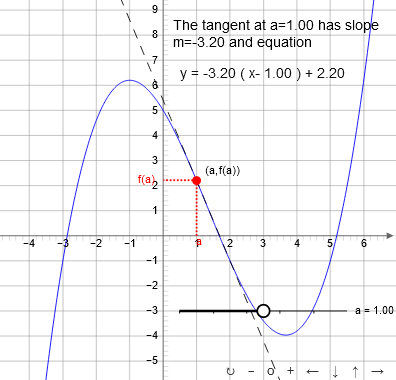
\includegraphics[width=\linewidth]{external/jsxgraph-slope-via-tangent.png}
\end{sbspanel}%
\begin{sbspanel}{0.21}%

\includegraphics[width=\linewidth]{generated/qrcode/sec_slope-6-9.png}
\href{http://webwork.bridgew.edu/oer/functions_at_work/sec_slope-6-9.html}{Standalone}%
\par
\href{http://webwork.bridgew.edu/oer/functions_at_work/sec_slope-6-9-if.html}{Embed}%
\end{sbspanel}%
\end{sidebyside}%
\par
Said another way, the \emph{slope of the tangent to \(f(x)\)} is a function of the point \(a\) where you are centering your approximation. For simplicity, we often denote this using the notation%
\begin{equation*}
f'(a) = \text{ the slope of the line tangent to the function }f(x)\text{ at }a
\end{equation*}
%
\begin{assemblage}{Summary}{Connecting Slope and Tangent Lines.}{assemblage-connectingslopeandtangent}%
%
\begin{enumerate}
\item{}Near a point \((a,f(a))\), the function \(f(x)\) is \alert{approximately equal to} the \emph{line tangent} to \(f\) at that point. Mathematically, this means%
\begin{equation*}
(\text{height on function }f) \approx (\text{height on tangent line centered at } a)
\end{equation*}
for all values of \(x\) near to \(a\)%
\item{}It follows that the \alert{slope} of the function \(f\) at \(a\) is approximately equal to the \alert{slope} of the tangent at the point.  In other words,%
\begin{equation*}
(\text{slope of }y=f(x) \text{ at }x=a) \approx (\text{slope of the *tangent* to } f \text{ at } a)
\end{equation*}
%
\end{enumerate}
%
\end{assemblage}
This observation is very powerful, and it works in two directions.  For now, we will see how to use tangent lines to help us to \emph{approximate} the slope of a curve \(y=f(x)\) at various values of \(a\).%
\par
Later, we will see how to compute the slope of \(f(x)\) \emph{precisely} at some point \(a\).  As a result, we will also have found the slope of the \emph{line tangent} to the function at that value of \(a\).%
\begin{exploration}{Exploration}{}{ex_slope_from_graph}%
A function \(y=f(x)\) is defined using the graph below.%
\begin{image}{0.2}{0.6}{0.2}{}%
\resizebox{\linewidth}{!}{%
\def\drawtikzspline(#1,#2,#3,#4,#5,#6){ \draw[curve,domain=(#1):(#4)] plot (\x , { ( (((#3) + (#6))*(#1) - ((#3) + (#6))*(#4) - 2*(#2) + 2*(#5))/((#1)^3 - 3*((#1)^2)*(#4) + 3*(#1)*((#4)^2) - (#4)^3) )*((\x)^3) + ( -(((#3) + 2*(#6))*((#1)^2) + ((#3) - (#6))*(#1)*(#4) - (2*(#3) + (#6))*((#4)^2) - 3*((#1) + (#4))*(#2) + 3*((#1) + (#4))*(#5))/((#1)^3 - 3*((#1)^2)*(#4) + 3*(#1)*((#4)^2) - (#4)^3) ) *((\x)^2) + ( ((#6)*((#1)^3) + (2*(#3) + (#6))*((#1)^2)*(#4) - ((#3) + 2*(#6))*(#1)*((#4)^2) - (#3)*((#4)^3) - 6*(#1)*(#4)*(#2) + 6*(#1)*(#4)*(#5))/((#1)^3 - 3*((#1)^2)*(#4) + 3*(#1)*((#4)^2) - (#4)^3) ) * (\x) + ( -((#6)*((#1)^3)*(#4) + ((#3) - (#6))*((#1)^2)*(#4)^2 - (#3)*(#1)*((#4)^3) - (3*(#1)*((#4)^2) - (#4)^3)*(#2) - ((#1)^3 - 3*((#1)^2)*(#4))*(#5))/((#1)^3 - 3*((#1)^2)*(#4) + 3*(#1)*((#4)^2) - (#4)^3))}) }

\begin{tikzpicture}
  \draw[axes] (-2,0)--(5,0);
  \draw[axes] (0,-2)--(0,5);
  \draw[grid] (-1.5,4.5) grid (4.5,-1.5);
  
  \drawtikzspline(0,1,0.5,1,3,1);
  \drawtikzspline(1,3,1,2,3.75,0);
  \drawtikzspline(2,3.75,0,3,0.5,-1);
  \drawtikzspline(3,0.5,-1,4,-0.5,0);
  \drawtikzspline(4,-0.5,0,5,-1,-1);

\end{tikzpicture}
}%
\end{image}%
\begin{enumerate}[font=\bfseries,label=(\alph*),ref=\alph*]%
\item{}Approximate the slope to the function \(y=f(x)\) at the point \(a=1\)%
\par\smallskip%
\noindent\textbf{\blocktitlefont Solution}.\hypertarget{ex_slope_from_graph-2-2}{}\quad{}We will approximate the slope at a value of \(a\) by first drawing the tangent to the curve at that point.%
\begin{sidebyside}{2}{0.075}{0.075}{0.17}%
\begin{sbspanel}{0.47}%
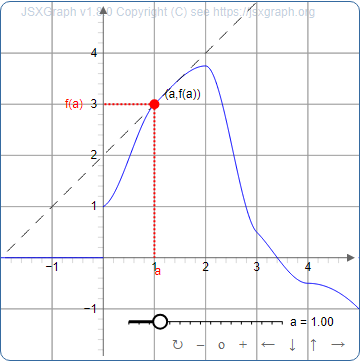
\includegraphics[width=\linewidth]{generated/preview/ex_slope_from_graph-2-2-2-preview.png}
\end{sbspanel}%
\begin{sbspanel}{0.21}%

\includegraphics[width=\linewidth]{generated/qrcode/ex_slope_from_graph-2-2-2.png}
\href{http://webwork.bridgew.edu/oer/functions_at_work/ex_slope_from_graph-2-2-2.html}{Standalone}%
\par
\href{http://webwork.bridgew.edu/oer/functions_at_work/ex_slope_from_graph-2-2-2-if.html}{Embed}%
\end{sbspanel}%
\end{sidebyside}%
\par
We can then find two points \alert{on the line} and use the slope formula%
\begin{equation*}
m = \dfrac{\Delta y}{\Delta x} = \dfrac{y_2-y_1}{x_2-x_1}
\end{equation*}
Note that these points will not be on the original curve, since we are technically finding the slope of the \emph{tangent line}, which we are only using to \alert{approximate} the real curve.%
\par
To find the tangent to a curve at a point, take a ruler and "line it up" with the curve at that point. The interactive graphic below shows the line you would get at each point.%
\par
To find the slope of \(f\) at \(a=1\), find the tangent to \(f\) at \(a=1\). Find two points on this tangent line.  One is \((1,3)\), and another is \((0,2)\). The slope of the line between these lines is%
\begin{equation*}
m = \dfrac{3-2}{1-0} = \dfrac{1}{1} = 1
\end{equation*}
Therefore, the slope of \(f(x)\) at \(a=1\) is equal to 1.%
\item{}Approximate the slope to the function \(y=f(x)\) at the point \(a=2\)%
\par\smallskip%
\noindent\textbf{\blocktitlefont Solution}.\hypertarget{ex_slope_from_graph-3-2}{}\quad{}We will approximate the slope at a value of \(a\) by first drawing the tangent to the curve at that point.%
\begin{sidebyside}{2}{0.075}{0.075}{0.17}%
\begin{sbspanel}{0.47}%
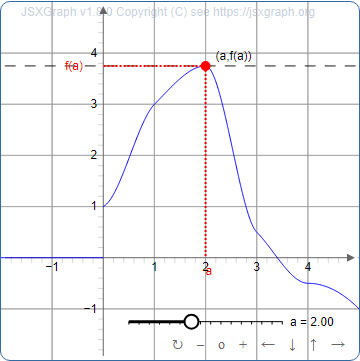
\includegraphics[width=\linewidth]{generated/preview/ex_slope_from_graph-3-2-2-preview.png}
\end{sbspanel}%
\begin{sbspanel}{0.21}%

\includegraphics[width=\linewidth]{generated/qrcode/ex_slope_from_graph-3-2-2.png}
\href{http://webwork.bridgew.edu/oer/functions_at_work/ex_slope_from_graph-3-2-2.html}{Standalone}%
\par
\href{http://webwork.bridgew.edu/oer/functions_at_work/ex_slope_from_graph-3-2-2-if.html}{Embed}%
\end{sbspanel}%
\end{sidebyside}%
\par
We can then find two points \alert{on the line} and use the slope formula%
\begin{equation*}
m = \dfrac{\Delta y}{\Delta x} = \dfrac{y_2-y_1}{x_2-x_1}
\end{equation*}
Note that these points will not be on the original curve, since we are technically finding the slope of the \emph{tangent line}, which we are only using to \alert{approximate} the real curve.%
\par
To find the tangent to a curve at a point, take a ruler and "line it up" with the curve at that point. The interactive graphic below shows the line you would get at each point.%
\par
To find the slope of \(f\) at \(a=2\), first, draw the line tangent to \(f(x)\) at \(a=2\), and find two points on that line. One point is \((2,3.75)\), and another is \((0,3.75)\) The slope of the line between these lines is%
\begin{equation*}
m = \dfrac{3.75-3.75}{2-0} = \dfrac{0}{2} = 0
\end{equation*}
Therefore, the slope of \(f(x)\) at \(a=2\) is equal to 0.%
\item{}Approximate the slope to the function \(y=f(x)\) at the point \(a=3\)%
\par\smallskip%
\noindent\textbf{\blocktitlefont Solution}.\hypertarget{ex_slope_from_graph-4-2}{}\quad{}We will approximate the slope at a value of \(a\) by first drawing the tangent to the curve at that point.%
\begin{sidebyside}{2}{0.075}{0.075}{0.17}%
\begin{sbspanel}{0.47}%
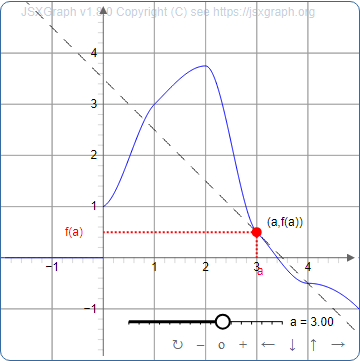
\includegraphics[width=\linewidth]{generated/preview/ex_slope_from_graph-4-2-2-preview.png}
\end{sbspanel}%
\begin{sbspanel}{0.21}%

\includegraphics[width=\linewidth]{generated/qrcode/ex_slope_from_graph-4-2-2.png}
\href{http://webwork.bridgew.edu/oer/functions_at_work/ex_slope_from_graph-4-2-2.html}{Standalone}%
\par
\href{http://webwork.bridgew.edu/oer/functions_at_work/ex_slope_from_graph-4-2-2-if.html}{Embed}%
\end{sbspanel}%
\end{sidebyside}%
\par
We can then find two points \alert{on the line} and use the slope formula%
\begin{equation*}
m = \dfrac{\Delta y}{\Delta x} = \dfrac{y_2-y_1}{x_2-x_1}
\end{equation*}
Note that these points will not be on the original curve, since we are technically finding the slope of the \emph{tangent line}, which we are only using to \alert{approximate} the real curve.%
\par
To find the tangent to a curve at a point, take a ruler and "line it up" with the curve at that point. The interactive graphic below shows the line you would get at each point.%
\par
To find the slope of \(f\) at \(a=3\), first, draw the line tangent to \(f(x)\) at \(a=3\), and find two points on that line. One point is \((3,0.5)\), and another is \((0,3.5)\) The slope of the line between these lines is%
\begin{equation*}
m = \dfrac{0.5-3.5}{3-0} = \dfrac{-3}{3} = -1
\end{equation*}
Therefore, the slope of \(f(x)\) at \(a=3\) is equal to -1.%
\item{}Approximate the slope to the function \(y=f(x)\) at the point \(a=4\)%
\par\smallskip%
\noindent\textbf{\blocktitlefont Solution}.\hypertarget{ex_slope_from_graph-5-2}{}\quad{}We will approximate the slope at a value of \(a\) by first drawing the tangent to the curve at that point.%
\begin{sidebyside}{2}{0.075}{0.075}{0.17}%
\begin{sbspanel}{0.47}%
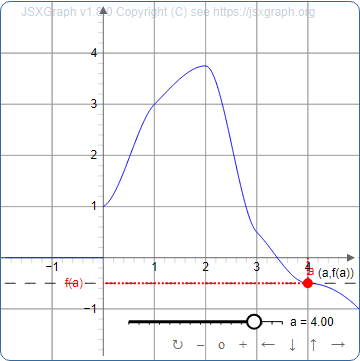
\includegraphics[width=\linewidth]{generated/preview/ex_slope_from_graph-5-2-2-preview.png}
\end{sbspanel}%
\begin{sbspanel}{0.21}%

\includegraphics[width=\linewidth]{generated/qrcode/ex_slope_from_graph-5-2-2.png}
\href{http://webwork.bridgew.edu/oer/functions_at_work/ex_slope_from_graph-5-2-2.html}{Standalone}%
\par
\href{http://webwork.bridgew.edu/oer/functions_at_work/ex_slope_from_graph-5-2-2-if.html}{Embed}%
\end{sbspanel}%
\end{sidebyside}%
\par
We can then find two points \alert{on the line} and use the slope formula%
\begin{equation*}
m = \dfrac{\Delta y}{\Delta x} = \dfrac{y_2-y_1}{x_2-x_1}
\end{equation*}
Note that these points will not be on the original curve, since we are technically finding the slope of the \emph{tangent line}, which we are only using to \alert{approximate} the real curve.%
\par
To find the tangent to a curve at a point, take a ruler and "line it up" with the curve at that point. The interactive graphic below shows the line you would get at each point.%
\par
To find the slope of \(f\) at \(a=4\), first, draw the line tangent to \(f(x)\) at \(a=4\), and find two points on that line. One point is \((4,-0.5)\), and another is \((0,-0.5)\) The slope of the line between these lines is%
\begin{equation*}
m = \dfrac{0.5-(-0.5)}{4-0} = \dfrac{0}{4} = 0
\end{equation*}
Therefore, the slope of \(f(x)\) at \(a=4\) is equal to 0.%
\end{enumerate}%
\end{exploration}%
\end{subsectionptx}
\end{sectionptx}
%
%
\typeout{************************************************}
\typeout{Section 9.2 Approximating Slope with Secant Lines}
\typeout{************************************************}
%
\begin{sectionptx}{Section}{Approximating Slope with Secant Lines}{}{Approximating Slope with Secant Lines}{}{}{sec_secantangent}
\begin{sidebyside}{2}{0}{0}{0}%
\begin{sbspanel}{0.5}%
Given a function \(f(x)\), and an \(x\) value \(a\), we want to find the slope of \(f\) at \(a\). Unfortunately, you need \emph{two points} to define a line, but a tangent line usualy only touches the curve at \emph{one point}. To help us define slope precisely, we will need a new concept.%
\end{sbspanel}%
\begin{sbspanel}{0.5}%
\resizebox{\linewidth}{!}{%
   \def\drawtikzspline(#1,#2,#3,#4,#5,#6){ \draw[curve,domain=(#1):(#4)] plot (\x , { ( (((#3) + (#6))*(#1) - ((#3) + (#6))*(#4) - 2*(#2) + 2*(#5))/((#1)^3 - 3*((#1)^2)*(#4) + 3*(#1)*((#4)^2) - (#4)^3) )*((\x)^3) + ( -(((#3) + 2*(#6))*((#1)^2) + ((#3) - (#6))*(#1)*(#4) - (2*(#3) + (#6))*((#4)^2) - 3*((#1) + (#4))*(#2) + 3*((#1) + (#4))*(#5))/((#1)^3 - 3*((#1)^2)*(#4) + 3*(#1)*((#4)^2) - (#4)^3) ) *((\x)^2) + ( ((#6)*((#1)^3) + (2*(#3) + (#6))*((#1)^2)*(#4) - ((#3) + 2*(#6))*(#1)*((#4)^2) - (#3)*((#4)^3) - 6*(#1)*(#4)*(#2) + 6*(#1)*(#4)*(#5))/((#1)^3 - 3*((#1)^2)*(#4) + 3*(#1)*((#4)^2) - (#4)^3) ) * (\x) + ( -((#6)*((#1)^3)*(#4) + ((#3) - (#6))*((#1)^2)*(#4)^2 - (#3)*(#1)*((#4)^3) - (3*(#1)*((#4)^2) - (#4)^3)*(#2) - ((#1)^3 - 3*((#1)^2)*(#4))*(#5))/((#1)^3 - 3*((#1)^2)*(#4) + 3*(#1)*((#4)^2) - (#4)^3))}) }
   \begin{tikzpicture}
     \draw[axes] (-1,0)--(4,0);
     \draw[axes] (0,-1)--(0,4);
     
     \drawtikzspline(-1,1,-1,2,2,1);
\drawtikzspline(2,2,1,4,2.5,-1);

     \draw [curve,domain=0.25:4,color=blue] plot ({\x},{(\x-2)+2}) node[right] {line approximating $f$ at $a$}; 
     \filldraw [color=red] (2,2) circle (2pt);
     \node [below,color=red] at (2,0) {$a$};
     \node [left,color=red] at (0,2) {$f(a)$};
     \draw[dashed,color=red] (2,0) -- (2,2) -- (0,2);

   \end{tikzpicture}
}%
\end{sbspanel}%
\end{sidebyside}%
\begin{definition}{Definition}{}{def-secant}%
\begin{sidebyside}{2}{0}{0}{0}%
\begin{sbspanel}{0.5}%
The \terminology{secant line} to \(f\) \terminology{at \(a,b\)} is the line that passes through the graph of \(y=f(x)\) at \(x=a\) and \(x=b\).%
\end{sbspanel}%
\begin{sbspanel}{0.5}%
\resizebox{\linewidth}{!}{%
\def\drawtikzspline(#1,#2,#3,#4,#5,#6){ \draw[curve,domain=(#1):(#4)] plot (\x , { ( (((#3) + (#6))*(#1) - ((#3) + (#6))*(#4) - 2*(#2) + 2*(#5))/((#1)^3 - 3*((#1)^2)*(#4) + 3*(#1)*((#4)^2) - (#4)^3) )*((\x)^3) + ( -(((#3) + 2*(#6))*((#1)^2) + ((#3) - (#6))*(#1)*(#4) - (2*(#3) + (#6))*((#4)^2) - 3*((#1) + (#4))*(#2) + 3*((#1) + (#4))*(#5))/((#1)^3 - 3*((#1)^2)*(#4) + 3*(#1)*((#4)^2) - (#4)^3) ) *((\x)^2) + ( ((#6)*((#1)^3) + (2*(#3) + (#6))*((#1)^2)*(#4) - ((#3) + 2*(#6))*(#1)*((#4)^2) - (#3)*((#4)^3) - 6*(#1)*(#4)*(#2) + 6*(#1)*(#4)*(#5))/((#1)^3 - 3*((#1)^2)*(#4) + 3*(#1)*((#4)^2) - (#4)^3) ) * (\x) + ( -((#6)*((#1)^3)*(#4) + ((#3) - (#6))*((#1)^2)*(#4)^2 - (#3)*(#1)*((#4)^3) - (3*(#1)*((#4)^2) - (#4)^3)*(#2) - ((#1)^3 - 3*((#1)^2)*(#4))*(#5))/((#1)^3 - 3*((#1)^2)*(#4) + 3*(#1)*((#4)^2) - (#4)^3))}) }
\begin{tikzpicture}
  \draw[axes] (-1,0)--(4,0);
  \draw[axes] (0,-1)--(0,4);
  
  \drawtikzspline(-1,1,-1,2,2,1);
  \drawtikzspline(2,2,1,4,2.5,-1);

  \draw [curve,domain=0.25:4,color=blue] plot ({\x},{0.25*(\x-2)+2}) node[right] {secant to $f$ at $a,b$}; 
  \filldraw [color=red] (2,2) circle (2pt);
  \node [below,color=red] at (2,0) {$a$};
  \node [left,color=red] at (0,2) {$f(a)$};
  \filldraw [color=red] (4,2.5) circle (2pt);
  \node [below,color=red] at (4,0) {$b$};
  \node [left,color=red] at (0,2.5) {$f(b)$};
  \draw[dashed,color=red] (2,0) -- (2,2) -- (0,2);
  \draw[dashed,color=red] (4,0) -- (4,2.5) -- (0,2.5);

\end{tikzpicture}
}%
\end{sbspanel}%
\end{sidebyside}%
\par
Furthermore, the \emph{slope} of the secant to \(f\) at \(a,b\) is equal to%
\begin{equation*}
\dfrac{f(b)-f(a)}{b-a} = \dfrac{\Delta y}{\Delta x}
\end{equation*}
%
\end{definition}
The key idea thing to notice is that when \(b\) is \emph{very close} to \(a\), then the secant line is \emph{very close} to the tangent line.%
\begin{sidebyside}{2}{0.075}{0.075}{0.17}%
\begin{sbspanel}{0.47}%
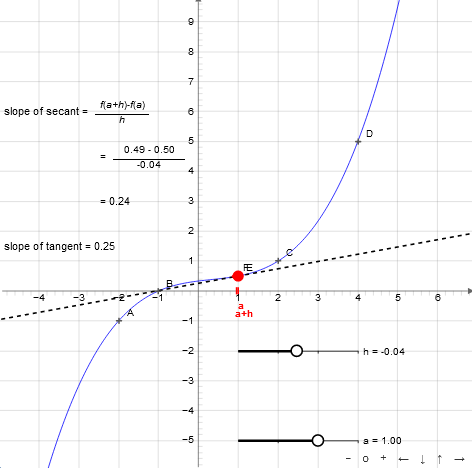
\includegraphics[width=\linewidth]{external/jsxgraph-derivative-limit-of-secant.png}
\end{sbspanel}%
\begin{sbspanel}{0.21}%

\includegraphics[width=\linewidth]{generated/qrcode/sec_secantangent-5.png}
\href{http://webwork.bridgew.edu/oer/functions_at_work/sec_secantangent-5.html}{Standalone}%
\par
\href{http://webwork.bridgew.edu/oer/functions_at_work/sec_secantangent-5-if.html}{Embed}%
\end{sbspanel}%
\end{sidebyside}%
\begin{exploration}{Exploration}{}{ex_approx_slope_from_secant}%
Let \(f(x) = x^2 + 2x\).  We want to study the function at \(a=3\).%
\begin{enumerate}[font=\bfseries,label=(\alph*),ref=\alph*]%
\item{}Estimage the slope of \(f\) at \(a=3\) by computing the slope of the secant between \(a=3\) and a value \(b\) that is 0.1 units away, 0.01 units away, and 0.001 units away.%
\par\smallskip%
\noindent\textbf{\blocktitlefont Solution}.\hypertarget{ex_approx_slope_from_secant-2-2}{}\quad{}Compute the average rate of change \(\dfrac{\Delta y}{\Delta x}\) over the intervals \([3,3.1]\), \([3,3.01]\), and \([3,3.001]\). In other words, we have the \(x\) values, so we need to find the \(y\) values, the changes \(\Delta x\) and \(\Delta y\), and then divide those changes to get the average change \(\frac{\Delta y}{\Delta x}\).%
\par
\begin{center}%
{\tabularfont%
\begin{tabular}{lBlBlBlBlBlBl}
\(x_1\)&\(x_2\)&\(\Delta x\)&\(y_1\)&\(y_2\)&\(\Delta y\)&\(\Delta y/\Delta x\)\tabularnewline\hrulemedium
\(3\)&\(\color{red} 3.1\)&\(0.1\)&\(\color{blue} f(3) = 3^2 + 2\cdot 3 = 15 \)&\(\color{blue} f(3.1) = 3.1^2 + 2\cdot 3.1 = 15.81\)&\(\color{green} y_2 - y_1 = 15.81-15 = 0.81\)&\(\Delta y/\Delta x = 0.81/0.1 = 8.1\)\tabularnewline\hrulemedium
\(3\)&\(\color{red} 3.01\)&\(0.01\)&\(\color{blue} f(3) = 3^2 + 2\cdot 3 = 15 \)&\(\color{blue} f(3.01) = 3.01^2 + 2\cdot 3.01 = 15.0801\)&\(\color{green} y_2 - y_1 = 15.81-15 = 0.0801\)&\(\Delta y/\Delta x = 0.0801/0.01 = 8.01\)\tabularnewline\hrulemedium
\(3\)&\(\color{red} 3.001\)&\(0.001\)&\(\color{blue} f(3) = 3^2 + 2\cdot 3 = 15 \)&\(\color{blue} f(3.001) = 3.001^2 + 2\cdot 3.001 = 15.008001\)&\(\color{green} y_2 - y_1 = 15.81-15 = 0.008001\)&\(\Delta y/\Delta x = 0.008001/0.001 = 8.001\)
\end{tabular}
}%
\end{center}%
%
\par
To interpret this table, note that the top row is an approximation of the slope where the points are reasonably far apart (\(\Delta x=0.1\)). In the middle row the points are closer together (\(\Delta x = 0.01\)), and in the bottom row the points are very close together (\(\Delta x = 0.001\)).%
\par
In other words, as you move from the top to bottom, the approximating line gets closer and closer to the function.%
\par
As the approximation improves, the "estimated slope" decreases from 8.1 to 8.01 to 8.001.  It looks like the slopes are getting \emph{closer and closer} to a slope of exactly \(m=8\) at \(a=3\).%
\item{}Use this slope to find an equation for the line tangent to \(f\) at \(a=3\).%
\par\smallskip%
\noindent\textbf{\blocktitlefont Solution}.\hypertarget{ex_approx_slope_from_secant-3-2}{}\quad{}To find the equation of a line, start by writing down the point-slope form%
\begin{equation*}
y = {\color{red} m } ( x - {\color{red} x_1} ) + {\color{red} y_1}
\end{equation*}
We are given that the x-value is  \(\color{red} x_1=3\). Plug this into the equation for the function \(f(x) = x^2 - 2x\) to get \(\color{red} y_1 = f(3) = 3^2 - 2\cdot 3 = 15\).%
\par
The only remaining number to find is the slope of the function \(\color{red} m\).  But we have already found above that the slope of the function at \(a=3\) is \(8\).  And the slope of the tangent equals the slope of the function, so we have that \(\color{red} m = 8\).%
\par
Putting this together, the slope of the line tangent to \(f\) at 3 is%
\begin{equation*}
y = {\color{red} 8 }( x - {\color{red} 3}) + {\color{red} 15}
\end{equation*}
This is the equation for the line that approximates \(f\) at the point \(a=3\).%
\end{enumerate}%
\end{exploration}%
\begin{assemblage}{Summary}{Secant Lines, AROC, and Slope.}{assemblage-secantlines}%
%
\begin{itemize}[label=\textbullet]
\item{}Just as we will use \emph{tangent lines} to approximate the original function, we will \emph{secant lines} to approximate tangent lines.%
\item{}The \emph{Average Rate of Change} (AROC) is defined to be \(\frac{\Delta y}{\Delta x}\). To compute the average rate of change just compute the height of your function at the given \(x\) values, and divide by the difference between those \(x\) values.%
\item{}We often use a table to help us compute the average rate of change, and call these AROC tables.  These are simply a way of organizing the different parts of computing   \(\frac{\Delta y}{\Delta x}\) for various values of \(x_1\) and \(x_2\).%
\begin{center}%
{\tabularfont%
\begin{tabular}{lBlBlBlBlBlBl}
\(x_1\)&\(x_2\)&\(\Delta x\)&\(y_1\)&\(y_2\)&\(\Delta y\)&\(\Delta y/\Delta x\)\tabularnewline\hrulemedium
\(a\)&\(b\)&\(\color{red} b-a\)&\(\color{blue} f(a) \)&\(\color{blue} f(b) \)&\(\color{green} f(b) - f(a) \)&\(\Big(f(b) - f(a)\Big)/\Big(b-a\Big) \)\tabularnewline\hrulemedium
\(c\)&\(d\)&\(\color{red} d-c\)&\(\color{blue} f(c) \)&\(\color{blue} f(d) \)&\(\color{green} f(d) - f(c) \)&\(\Big(f(d) - f(c)\Big)/\Big(d-c\Big) \)\tabularnewline\hrulemedium
\(\dots\)&\(\dots\)&\(\dots\)&\(\dots\)&\(\dots\)&\(\dots\)&\(\dots\)
\end{tabular}
}%
\end{center}%
\item{}Suppose you are \emph{given} a function \(f(x)\) and an \(x\)-value \(a\). To \emph{approximate the slope of \(f(x)\) at \(a\)}, create an AROC table as follows:%
\begin{enumerate}
\item{}Set \(x_1=a\) in each row. Pick several values for \(\Delta x\) that get smaller and smaller (think \(0.1\), \(0.01\), \(\dots\)). Put the largest \(\Delta x\) in the top row, and put smaller \(\Delta x \) in lower rows. For each row, set \(x_2 = x_1 + \Delta x\)%
\item{}Fill in the table, computing \(y_1,y_2,\Delta y,\) and \(\frac{\Delta y}{\Delta x}\).%
\item{}Read the right hand of the table from top to bottom.  Where is the average rate \(\frac{\Delta y}{\Delta x}\) going as \(\Delta x\rightarrow 0\)?%
\end{enumerate}
%
\end{itemize}
%
\end{assemblage}
The above process for approximating slope is the most accurate way of doing things, but it can be a bit involved. In specific circumstances, you can often \emph{approximate} the slope using a single computation.  Instead of repeatedly calculating \(\Delta y/\Delta x\) for smaller and smaller values of \(\Delta x\), you can sometimes pick a single very small value for \(\Delta x\). For example, picking \(\Delta x = 0.001\) gives us%
\begin{equation*}
\text{slope of f at }a \approx \dfrac{f(a+0.001) - f(a) }{0.001}
\end{equation*}
That value is only \emph{approximate}, so it might be too large and it might be too small. By using an AROC table, we get a better sense of whether the exact slope is smaller or larger.%
\end{sectionptx}
%
%
\typeout{************************************************}
\typeout{Section 9.3 Defining Slope Algebraically}
\typeout{************************************************}
%
\begin{sectionptx}{Section}{Defining Slope Algebraically}{}{Defining Slope Algebraically}{}{}{sec_slopealgebraically}
In the previous section, we developed a method that allows us to approximate slope by an iterative process of seeing where \emph{average slope is going} as the change in input \emph{\(\Delta x\) goes to zero}.%
\par
Using the language of \hyperref[ch_limits]{Chapter~{\xreffont\ref{ch_limits}}}, we can translate this into a limit definition of slope.%
\begin{definition}{Definition}{}{def-slopeAsLimit}%
Given a function \(f(x)\) and a number \(a\). The \terminology{slope of f at a}, abbreviated \(f'(a)\) is equal to%
\begin{equation*}
f'(a) = \lim_{\Delta x\rightarrow 0}\dfrac{\Delta y}{\Delta x} = \lim_{\Delta x\rightarrow 0} \dfrac{ f\Big(a+\Delta x\Big) - f\Big(a\Big) }{\Delta x} 
\end{equation*}
English keyboards do not have a button for \(\Delta x\), so we can use the letter \(h\) to abbreviate the change in the input.  This gives us an alternative form:%
\begin{equation*}
f'(a) = \displaystyle \lim_{h\rightarrow 0}\dfrac{f\Big(a+h\Big) - f\Big(a\Big) }{h} 
\end{equation*}
%
\end{definition}
To \emph{use} the limit definition,%
\begin{enumerate}
\item{}Completely simplify the fraction using the specific function \(f\) and number \(a\) that you are given.%
\item{}Compute the limit of the simplified function by letting \(h\) go to \(0\). For the purposes of this course, this means plugging in \(h=0\) as long as this does not result in division by \(0\).%
\end{enumerate}
%
\begin{exploration}{Exploration}{}{ex_slope_from_limit_defn}%
Let \(f(x) = x^2 + 2x\). Use the limit definition to find the slope of \(f\) at \(a=3\).%
\par\smallskip%
\noindent\textbf{\blocktitlefont Solution}.\hypertarget{ex_slope_from_limit_defn-2}{}\quad{}The limit definnition of slope at \(3\) gives us%
\begin{equation*}
\text{slope at 3 } = \lim_{\Delta x\rightarrow 0} \dfrac{\Delta y}{\Delta x} = \lim_{h\rightarrow 0} \dfrac{ {\color{blue}f\Big(3+h\Big)} - {\color{red} f\Big(3\Big)}}{h}
\end{equation*}
This function includes several components, that we first simplify on their own. The function is defined by the rule  \(f(x) = x^2 + 2x\).  That means that \(\color{red} f(3) = 3^2 + 2\cdot 3 = \dots = 15\). Similarly, we can simplify the expression as follows:%
\begin{align*}
\color{blue} f\Big(3+h\Big) \amp \color{blue} = \Big(3+h\Big)^2 + 2\cdot \Big(3+h\Big) \\
\amp \color{blue} = \Big(3+h\Big)\cdot\Big(3+h\Big)  + 2\cdot \Big(3+h\Big) \\
\amp \color{blue} = 9 + 3h + 3h + h^2 + 6 + 2h  \\
\color{blue} f\Big(3+h\Big) \amp = \color{blue} 15 + 8h + h^2   
\end{align*}
We can now plug these simplified expressions back into our limit definition%
\begin{align*}
\text{slope at 3 } \amp = \lim_{h\rightarrow 0} \dfrac{ {\color{blue}f\Big(3+h\Big)} - {\color{red} f\Big(3\Big)}}{h}\\
\amp = \lim_{h\rightarrow 0} \dfrac{ {\color{blue} (15 + 8h + h^2)}  - {\color{red} (15) } }{h}
\end{align*}
It is tempting to try to plug in \(h=0\), but if you do that on your calculator, you end up dividing by 0, which gives a value of \(UNDEFINED\) or \(DNE\). Because of this, we need to keep simplifying as in \hyperref[sec-combining_functions]{Section~{\xreffont\ref{sec-combining_functions}}}:%
\begin{align*}
\amp = \lim_{h\rightarrow 0} \dfrac{ 8h + h^2 }{h}\\
\amp = \lim_{h\rightarrow 0} \dfrac{ {\color{red} h}\cdot (8 + h)  }{{\color{red} h}}\\
\amp = \lim_{h\rightarrow 0} \dfrac{ (8 + h) }{1}\\
\amp = \lim_{h\rightarrow 0} (8 + h) 
\end{align*}
As \(h\rightarrow 0 \), the expression  \(8+h\) goes to \(8+0=8\).  In other words, the slope of \(f\) at \(a=3\) is exactly \(m=8\).%
\end{exploration}%
Our goal in this course is to use mathematics as a tool to deepen our understanding of economics and business concepts. One of the most important insights from the limit definition of slope is the following result.%
\begin{corollary}{Corollary}{}{}{cor-unitsofslope}%
Suppose that \(y=f(x)\) is a function, and that there are units for both the input \(x\) and output \(f\).  The following are \alert{always equal}%
\begin{itemize}[label=\textbullet]
\item{}The slope of \(f\) at \(a\)%
\item{}The instantaneous rate of change (IROC) of \(f\) at \(a\)%
\end{itemize}
%
\par
Furthermore, the units of slope and the units of IROC are always%
\begin{equation*}
\dfrac{\text{units of y}}{\text{units of x}}
\end{equation*}
%
\end{corollary}
\begin{insight}{Application}{Units and applied slope.}{sec_slopealgebraically-9}%
%
\begin{itemize}[label=\textbullet]
\item{}If \(y\) gives the value of a stock in dollars as a function of the number of days \(x\), then you can always find \emph{how fast the stock is changing} by looking at the \emph{slope of the value function}. Furthermore, that slope is measured in \emph{dollars per day}.%
\item{}If \(y\) gives your milemarker on a highway as a function of the time \(x\) in hours, then you can always find \emph{how fast your position is changing} by looking at the \emph{slope of the position function}. Furthermore, that slope is measured in miles per hour.%
\end{itemize}
%
\end{insight}
\begin{exploration}{Exploration}{}{ex_iroc_from_limit_defn}%
Suppose that the profit of a certain oil investment is given by \(P(x) = -x^2 + 4x - 1\) in millions of \textdollar{} as a function of the number of gallons of oil \(x\) produced over the lifetime of the investment.%
\par
How fast is the profit changing when \(x=1\) million units?%
\par\smallskip%
\noindent\textbf{\blocktitlefont Solution}.\hypertarget{ex_iroc_from_limit_defn-2}{}\quad{}We are asked for the instantaneous rate of change of profit at \(a=1\). Because IROC is the same thing as slope, we can use the limit definion of slope.  In other words, we must compute \(\lim_{\Delta x\rightarrow 0}\dfrac{\Delta y}{\Delta x}\) at \(a=1\) using the formula%
\begin{equation*}
\lim_{h\rightarrow 0} \dfrac{ {\color{blue} P\Big(1 + h\Big)}- {\color{red} P\Big(1\Big)} }{h}
\end{equation*}
As before, we will first simplify the components of this expression separately, and only put them back together later on.%
\begin{equation*}
\color{red} P\Big(1\Big) = -\,1^2 + 4\cdot 1 - 1 = -1 + 4 -1 = 2
\end{equation*}
%
\begin{align*}
\color{blue} P\Big(1 + h\Big) \amp\color{blue} = -\Big(1 + h\Big)^2 + 4\Big(1 + h\Big) - 1
\end{align*}
%
\begin{gather*}
\color{blue} = -\Big(1 + h\Big)\cdot \Big(1 + h\Big) + 4\Big(1 + h\Big) - 1
\end{gather*}
%
\begin{gather*}
\color{blue} = -\Big(1 + 2h + h^2\Big) + 4\Big(1 + h\Big) - 1\\
\color{blue} = -1 - 2h - h^2 + 4 + 4h - 1\\
\color{blue} = - h^2  + 2h +2 
\end{gather*}
%
\par
Putting this back into the limit definition gives%
\begin{align*}
\text{IROC at 1 } \amp = \lim_{h\rightarrow 0} \dfrac{  {\color{blue}P\Big(1+h\Big)} - {\color{red} P\Big(1\Big)}  }{h}\\
\amp = \lim_{h\rightarrow 0} \dfrac{ {\color{blue} ( - h^2  + 2h +2 )} - {\color{red} (2) }  }{h}\\
\amp = \lim_{h\rightarrow 0} \dfrac{ - h^2  + 2h }{h}\\
\amp = \lim_{h\rightarrow 0} \dfrac{ {\color{red} h}\cdot(-h  + 2) }{\color{red} h}\\
\amp = \lim_{h\rightarrow 0} \dfrac{ (-h  + 2) }{1}\\
\amp = \lim_{h\rightarrow 0} (-h  + 2) \\
\amp =  (-0  + 2) = 2 
\end{align*}
%
\par
The rate of change in profit is 2 (million \textdollar{}) per (million gallons).  Simplifying the units, this tells us that the profit is changing by 2 dollars per gallon when \(x=1\) million gallons.%
\end{exploration}%
\end{sectionptx}
%
%
\typeout{************************************************}
\typeout{Section 9.4 Defining a Slope Function}
\typeout{************************************************}
%
\begin{sectionptx}{Section}{Defining a Slope Function}{}{Defining a Slope Function}{}{}{sec-slopefunction}
So far, we have seen how to understand, approximate, and define the slope of a function at a point \(a\). If you want to look at the slope of the function at a different point, you can redo all of the computations, only with a different number.%
\par
As you recompute the slope at different values, you will notice that there is a lot of repeated effort that seems very similar.  We can avoid that repeated effort by instead studying \terminology{slope functions}.%
\begin{definition}{Definition}{}{def-derivativefunction}%
Let \(f(x)\) be any function. The \terminology{derivative} of \(f\), written \(f'(x)\), is the function which, when given any number \(a\), outputs the \emph{slope} of the original function at \(a\).%
\end{definition}
\begin{exploration}{Exploration}{}{explore_derivativeofx2}%
The function \(f(x) = x^2\) is graphed below. \begin{sidebyside}{2}{0.075}{0.075}{0.17}%
\begin{sbspanel}{0.47}%
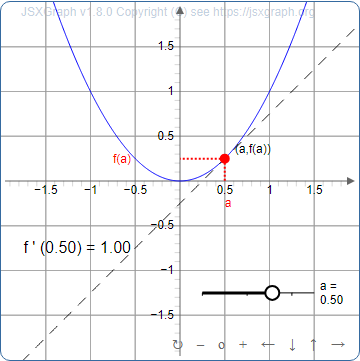
\includegraphics[width=\linewidth]{generated/preview/explore_derivativeofx2-1-1-2-preview.png}
\end{sbspanel}%
\begin{sbspanel}{0.21}%

\includegraphics[width=\linewidth]{generated/qrcode/explore_derivativeofx2-1-1-2.png}
\href{http://webwork.bridgew.edu/oer/functions_at_work/explore_derivativeofx2-1-1-2.html}{Standalone}%
\par
\href{http://webwork.bridgew.edu/oer/functions_at_work/explore_derivativeofx2-1-1-2-if.html}{Embed}%
\end{sbspanel}%
\end{sidebyside}%
%
\begin{enumerate}[font=\bfseries,label=(\alph*),ref=\alph*]%
\item{}Use the graph to approximate \(f'(-1)\), \(f'(0)\), \(f'(1)\).%
\par\smallskip%
\noindent\textbf{\blocktitlefont Solution}.\hypertarget{explore_derivativeofx2-2-2}{}\quad{}To find a slope from a graph, first draw the tangent line at that point. Then, find the slope of that tangent line.%
\par
In this interactive graphic, adjusting the slider draws the tangent line for you.%
\par
In either case, we see that%
\begin{equation*}
f'(-1) = -2\text{,}
\end{equation*}
%
\begin{equation*}
f'(0)=0\text{,}
\end{equation*}
%
\begin{equation*}
f'(1) = 2
\end{equation*}
%
\item{}Use the interactive graphic to come up with a \emph{conjecture} (educacted guess) for an equation for the \emph{slope function} \(f'(x)\).%
\par\smallskip%
\noindent\textbf{\blocktitlefont Solution}.\hypertarget{explore_derivativeofx2-3-2}{}\quad{}Try adjusting the value of \(x\), and look at what the slope ends up equaling.%
\par
No matter what value of \(x\) you end up selecting, it looks like the slope is exactly twice the \(x\) value. This leads to a conjecture that%
\begin{equation*}
f'(x) = 2x
\end{equation*}
%
\item{}Use the limit definition of the derivative to find an equation for \(f'(x)\)%
\par\smallskip%
\noindent\textbf{\blocktitlefont Solution}.\hypertarget{explore_derivativeofx2-4-2}{}\quad{}To apply the limit definition of slope to \emph{any} value of \(x\), we just need to write down the same formula, only using a variable \(x\) instead of a specific number \(a\).  In other words, we must compute%
\begin{equation*}
f'(x) =  \lim_{h\rightarrow 0} \dfrac{{\color{blue} f\Big(x+h\Big)} - {\color{red} f\Big(x\Big)} }{h}
\end{equation*}
As always, we simplify the corresponding expressions separately.  First, by definition \(\color{red} f(x) = x^2\).  This expression cannot be simplified further, so can now move onto the second expression%
\begin{align*}
\color{blue} f\Big(x+h\Big) \amp = \color{blue} (x+h)^2 \\
\amp = \color{blue} (x+h)\cdot (x+h) \\
\amp = \color{blue} x^2 + 2xh + h^2 
\end{align*}
This cannot be simplified further, so we can now plug our expressions back into the limit definition of slope%
\begin{align*}
f'(x) = \amp \lim_{h\rightarrow 0} \dfrac{{\color{blue} f\Big(x+h\Big)} - {\color{red} f\Big(x\Big)} }{h} \\
\amp =  \lim_{h\rightarrow 0}\dfrac{  {\color{blue} (x^2 + 2xh + h^2)} - {\color{red} (x^2)}  }{h}\\
\amp =  \lim_{h\rightarrow 0}\dfrac{  2xh + h^2  }{h} \\
\amp =  \lim_{h\rightarrow 0}\dfrac{  {\color{red} h}(2x + h)  }{\color{red} h} \\
\amp =  \lim_{h\rightarrow 0} (2x + h)  \\
f'(x) \amp =  2x  
\end{align*}
%
\item{}Find an equation for the line tangent to \(f(x) = x^2\) at \(10\).%
\par\smallskip%
\noindent\textbf{\blocktitlefont Solution}.\hypertarget{explore_derivativeofx2-5-2}{}\quad{}To find the equation for the tangent line, first write down point slope form of the line%
\begin{equation*}
y = {\color{red} m } (x - {\color{red} x_1}) + {\color{red} y_1}
\end{equation*}
We are given that \(x_1=10\). To find \(y_1\), find plug 10 into the equation for the \emph{original} function \(f(x)=x^2\)%
\begin{equation*}
y_1 = f(10) = 10^2 = 100
\end{equation*}
%
\par
We can't use the graph to find the slope of the functino at \(10\), so we either need to approximate the slope numerically, use the limit definition, \emph{or} use the equation for the slope function \(f'(x)\) that we have found above.%
\par
Since we know that the \emph{slope of \(f\) at \(x\)} is \(f'(x) = 2x\), we can find the slope at 10 by plugging 10 into the \emph{slope} or \emph{derivative} function \(f'(x)=2x\)%
\begin{equation*}
m = f'(10) = 2\cdot 10 = 20
\end{equation*}
Putting all of this into the point slope form, we get that the equation of the tangent line is%
\begin{equation*}
y = {\color{red} 20} (x - {\color{red} 10}) + {\color{red} 100} 
= 20x +80
\end{equation*}
%
\end{enumerate}%
\end{exploration}%
\begin{exploration}{Exploration}{}{ex_fprime_from_graph}%
A function \(y=f(x)\) is defined using the graph below.%
\begin{image}{0.125}{0.75}{0.125}{}%
\resizebox{\linewidth}{!}{%
\def\drawtikzspline(#1,#2,#3,#4,#5,#6){ \draw[curve,domain=(#1):(#4)] plot (\x , { ( (((#3) + (#6))*(#1) - ((#3) + (#6))*(#4) - 2*(#2) + 2*(#5))/((#1)^3 - 3*((#1)^2)*(#4) + 3*(#1)*((#4)^2) - (#4)^3) )*((\x)^3) + ( -(((#3) + 2*(#6))*((#1)^2) + ((#3) - (#6))*(#1)*(#4) - (2*(#3) + (#6))*((#4)^2) - 3*((#1) + (#4))*(#2) + 3*((#1) + (#4))*(#5))/((#1)^3 - 3*((#1)^2)*(#4) + 3*(#1)*((#4)^2) - (#4)^3) ) *((\x)^2) + ( ((#6)*((#1)^3) + (2*(#3) + (#6))*((#1)^2)*(#4) - ((#3) + 2*(#6))*(#1)*((#4)^2) - (#3)*((#4)^3) - 6*(#1)*(#4)*(#2) + 6*(#1)*(#4)*(#5))/((#1)^3 - 3*((#1)^2)*(#4) + 3*(#1)*((#4)^2) - (#4)^3) ) * (\x) + ( -((#6)*((#1)^3)*(#4) + ((#3) - (#6))*((#1)^2)*(#4)^2 - (#3)*(#1)*((#4)^3) - (3*(#1)*((#4)^2) - (#4)^3)*(#2) - ((#1)^3 - 3*((#1)^2)*(#4))*(#5))/((#1)^3 - 3*((#1)^2)*(#4) + 3*(#1)*((#4)^2) - (#4)^3))}) }

\begin{tikzpicture}
  \draw[axes] (-2,0)--(5,0);
  \draw[axes] (0,-2)--(0,5);
  \draw[grid] (-0.5,4.5) grid (7.5,-1.5);
  
  \drawtikzspline(0,2,-1,1,1,0);
  \drawtikzspline(1,1,0,2,2,1);
  \drawtikzspline(2,2,1,3,3,0);
  \drawtikzspline(3,3,0,4,1,-2);
  \drawtikzspline(4,1,-2,5,-1.25,0);
  \drawtikzspline(5,-1.25,0,6,-1,0.5);
  \drawtikzspline(6,-1,0.5,7,-0.5,0.5);

\end{tikzpicture}
}%
\end{image}%
\begin{enumerate}[font=\bfseries,label=(\alph*),ref=\alph*]%
\item{}Compute \(f'(0)\), \(f'(1)\), \(f'(2)\), \(f'(3)\), \(f'(4)\), \(f'(5)\), \(f'(6)\).%
\par\smallskip%
\noindent\textbf{\blocktitlefont Solution}.\hypertarget{ex_fprime_from_graph-2-2}{}\quad{}We will approximate the slope at a value of \(a\) by first drawing the tangent to the curve at that point, and using the fact that%
\begin{equation*}
\text{Slope of  } f \text{ at }a = \text{ Slope of line tangent to }f \text{ at }a
\end{equation*}
. To find the tangent to a curve at a point, take a ruler and "line it up" with the curve at that point. The interactive graphic below shows the line you would get at each point.%
\par
\begin{sidebyside}{2}{0.075}{0.075}{0.17}%
\begin{sbspanel}{0.47}%
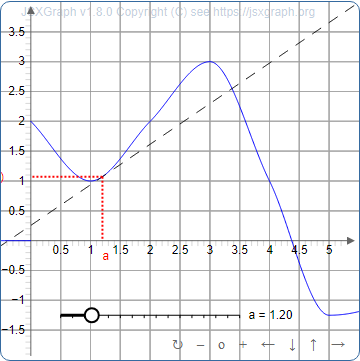
\includegraphics[width=\linewidth]{generated/preview/ex_fprime_from_graph-2-2-2-1-preview.png}
\end{sbspanel}%
\begin{sbspanel}{0.21}%

\includegraphics[width=\linewidth]{generated/qrcode/ex_fprime_from_graph-2-2-2-1.png}
\href{http://webwork.bridgew.edu/oer/functions_at_work/ex_fprime_from_graph-2-2-2-1.html}{Standalone}%
\par
\href{http://webwork.bridgew.edu/oer/functions_at_work/ex_fprime_from_graph-2-2-2-1-if.html}{Embed}%
\end{sbspanel}%
\end{sidebyside}%
%
\par
Using these tangent lines, you can determine that%
\begin{equation*}
f'(0) = -1
\end{equation*}
%
\begin{equation*}
f'(1) = 0
\end{equation*}
%
\begin{equation*}
f'(2) = 1
\end{equation*}
%
\begin{equation*}
f'(3) = 0
\end{equation*}
%
\begin{equation*}
f'(4) = -2
\end{equation*}
%
\begin{equation*}
f'(5) = 0
\end{equation*}
%
\begin{equation*}
f'(6) = 1/2
\end{equation*}
%
\item{}Find all points where the tangent is horizontal.%
\par\smallskip%
\noindent\textbf{\blocktitlefont Solution}.\hypertarget{ex_fprime_from_graph-3-2}{}\quad{}The tangent is horizontal at \(x\)\emph{if and only if} the slope of the function is equal to 0 at \(x\), \emph{if and only if} \(f'(x) = 0\).%
\par
This happens at the values \(x=1,3,5\), and at no other x-values.%
\item{}Find the intervals where \(f(x)\) is increasing.%
\par\smallskip%
\noindent\textbf{\blocktitlefont Solution}.\hypertarget{ex_fprime_from_graph-4-2}{}\quad{}The function is increasing \emph{if and only if} the slope of \(f\) at \(x\) is positive \emph{if and only if} \(f'(x)\gt 0\).%
\par
Looking at the graph, the slope is positive at to different parts of the graph:%
\begin{itemize}[label=\textbullet]
\item{}between \(x=1\) and \(x=3\)%
\item{}to the right of \(x=5\)%
\end{itemize}
In interval notation,  \(f\) is increasing on the interval \((1,3)\cup (5,\infty)\)%
\item{}Find the intervals where \(f(x)'\lt 0\).%
\par\smallskip%
\noindent\textbf{\blocktitlefont Solution}.\hypertarget{ex_fprime_from_graph-5-2}{}\quad{}The function is decreasing \emph{if and only if} the slope of \(f\) at \(x\) is negative \emph{if and only if} \(f'(x)\lt 0\).%
\par
Looking at the graph, the slope is negative at two different parts of the graph:%
\begin{itemize}[label=\textbullet]
\item{}to the left of \(x=1\)%
\item{}between \(x=3\) and \(x=5\)%
\end{itemize}
In interval notation,  \(f\) is decreasing on the interval \((-\infty,1)\cup (3,5)\)%
\item{}Draw a sketch of the slope function \(f'(x)\).%
\par\smallskip%
\noindent\textbf{\blocktitlefont Solution}.\hypertarget{ex_fprime_from_graph-6-2}{}\quad{}We have already computed the \emph{slope function} \(f'\) at x-values \(0,1,2,3,4,6\).  Summarizing that in a table, we have \begin{center}%
{\tabularfont%
\begin{tabular}{lBlBlBlBlBlBlBl}
\(x\)&\(0\)&\(1\)&\(2\)&\(3\)&\(4\)&\(5\)&\(6\)\tabularnewline\hrulemedium
\(f'(x)\)&\(-1\)&\(0\)&\(1\)&\(0\)&\(-2\)&\(-1.1\)&\(1/2\)
\end{tabular}
}%
\end{center}%
 To sketch the graph of the \emph{slope} as a function of \(x\), plot each of these \emph{slopes}, and then connect them with a reasonably smooth curve.%
\begin{image}{0.125}{0.75}{0.125}{}%
\resizebox{\linewidth}{!}{%
  \def\drawtikzspline(#1,#2,#3,#4,#5,#6){ \draw[curve,domain=(#1):(#4)] plot (\x , { ( (((#3) + (#6))*(#1) - ((#3) + (#6))*(#4) - 2*(#2) + 2*(#5))/((#1)^3 - 3*((#1)^2)*(#4) + 3*(#1)*((#4)^2) - (#4)^3) )*((\x)^3) + ( -(((#3) + 2*(#6))*((#1)^2) + ((#3) - (#6))*(#1)*(#4) - (2*(#3) + (#6))*((#4)^2) - 3*((#1) + (#4))*(#2) + 3*((#1) + (#4))*(#5))/((#1)^3 - 3*((#1)^2)*(#4) + 3*(#1)*((#4)^2) - (#4)^3) ) *((\x)^2) + ( ((#6)*((#1)^3) + (2*(#3) + (#6))*((#1)^2)*(#4) - ((#3) + 2*(#6))*(#1)*((#4)^2) - (#3)*((#4)^3) - 6*(#1)*(#4)*(#2) + 6*(#1)*(#4)*(#5))/((#1)^3 - 3*((#1)^2)*(#4) + 3*(#1)*((#4)^2) - (#4)^3) ) * (\x) + ( -((#6)*((#1)^3)*(#4) + ((#3) - (#6))*((#1)^2)*(#4)^2 - (#3)*(#1)*((#4)^3) - (3*(#1)*((#4)^2) - (#4)^3)*(#2) - ((#1)^3 - 3*((#1)^2)*(#4))*(#5))/((#1)^3 - 3*((#1)^2)*(#4) + 3*(#1)*((#4)^2) - (#4)^3))}) }              \begin{tikzpicture}
  \draw[axes] (-1,0) -- (7,0);
  \draw[axes] (0,-3) -- (0,3);
  \draw[grid] ( -0.5,3) grid (6.5,-3);

  \filldraw (0,-1) circle (3pt);
  \drawtikzspline(0,-1,0,1,0,1);
  \filldraw (1,0) circle (3pt);
  \drawtikzspline(1,0,1,2,1,0);
  \filldraw (2,1) circle (3pt);
  \drawtikzspline(2,1,0,3,0,-1.5);
  \filldraw (3,0) circle (3pt);
  \drawtikzspline(3,0,-1.5,4,-2,0);
  \filldraw (4,-2) circle (3pt);
  \drawtikzspline(4,-2,0,5,0,0.5);
  \filldraw (5,0) circle (3pt);
  \drawtikzspline(5,0,0.5,6,0.5,0);
  \filldraw (6,0.5) circle (3pt);

\end{tikzpicture}
}%
\end{image}%
\end{enumerate}%
\end{exploration}%
%
%
\typeout{************************************************}
\typeout{Subsection 9.4.1 Interpreting the Meaning of \(f'(x)\)}
\typeout{************************************************}
%
\begin{subsectionptx}{Subsection}{Interpreting the Meaning of \(f'(x)\)}{}{Interpreting the Meaning of \(f'(x)\)}{}{}{subsec-derivativenotation}
So far, we have focused on the graphical interpretation of the derivative function by emphasizing that for a graph \(y=f(x)\)%
\begin{equation*}
f'(a) = (\text{the slope of } f \text{ at }x_1=a)
\end{equation*}
But the true power of calculus comes from the \emph{many} applications of derivatives to \emph{other kinds of questions}. We have already seen this breifly in \hyperref[cor-unitsofslope]{Corollary~{\xreffont\ref{cor-unitsofslope}}}, but it will be helpful to expand on this in greater detail.%
\par
Perhaps the simplest way to understand the meaning of \(f'\) in different situations is to pay attention to the \emph{units of measurement} for \(f\) and \(f'\). For example, for a \emph{height function} \(y=f(x)\), the units of \(f\) might be meters or feet. On the other hand, for a \emph{profit function} \(P(x)\), the units of \(P\) might be dollars, or millions of dollars, or yuan.%
\par
The units of the input \(x\) also play an important part in the meaning of the function. There is a world of difference between moving 6 miles between \emph{hours} \(x_1=0\) and \(x_2=1\) (an average velocity of 6 miles per hour) and moving 6 miles between \emph{second} \(x_1=0\) and \(x_2=1\) (an average velocity of \emph{360} miles per hour).%
\par
To help us remember the units of derivatives, it is helpful to consider an alternate notation for the derivative function \(f'\). The key idea here is to realize that \(\Delta\) is the greek letter \(D\).  Since we use the blocky symbol \(\Delta\) to refer to approximate changes, we can instead use the smooth symbol \(d\) to refer to instantaneous changes.  This gives us the following notation.%
\begin{definition}{Definition}{}{def-dydx-notation}%
Let \(y=f(x)\) be any function.%
\par
Because \(f'(x) = \lim_{\Delta x\rightarrow 0} \dfrac{\Delta y}{\Delta x}\), we often write%
\begin{equation*}
f'(x) = \dfrac{df}{dx} = \dfrac{dy}{dx}
\end{equation*}
This notation helps us remember \hyperref[cor-unitsofslope]{Corollary~{\xreffont\ref{cor-unitsofslope}}}, which says%
\begin{equation*}
(\text{units of }f') = \dfrac{\text{units of f}}{\text{units of x}}
\end{equation*}
%
\end{definition}
For example, if \(C(x)\) is the \emph{total} (cumulative) cost in \textdollar{} of \(x\) items, then the \emph{rate of change} of cost (how fast the cost is changing)%
\begin{equation*}
C'(x) = \dfrac{dC}{dx} = \dfrac{\$}{\text{item}}
\end{equation*}
In other words, if you have a graph of total cost, the \emph{item cost} is equal to the \emph{slope of the graph}. We will return to this example in greater detail in \hyperref[sec-marginalcost]{Section~{\xreffont\ref{sec-marginalcost}}}%
\begin{assemblage}{Summary}{Interpreting Derivatives.}{assemblage_meaningofderivative}%
%
\begin{descriptionlist}
\begin{dlimedium}{Height Functions}{assemblage_meaningofderivative-2-1-1}%
Suppose that \(y=f(x)\) gives the \emph{height} of a hill in feet as a function of the horizontal position \(x\) in feet. Then \(f'(x)\) gives the \emph{slope} of the hill in \(\frac{meters}{meters}\) (meters-per-meter).%
\end{dlimedium}%
\begin{dlimedium}{Position Functions}{assemblage_meaningofderivative-2-1-2}%
Suppose that \(f(t)\) gives the \emph{position} of a vehicle in miles as a function of the current time \(t\) in hours. Then \(f'(t)\) gives the \emph{velocity} of the vehicle in \(\frac{miles}{hour}\) (miles per hour).%
\end{dlimedium}%
\begin{dlimedium}{Profit Functions}{assemblage_meaningofderivative-2-1-3}%
Suppose that \(P(x)\) gives the \emph{total profit} of a business in dollars as a function of the number of items \(x\) being sold. Then \(P'(x)\) tells you  \emph{how fast Profit changes} in \(\frac{dollars}{item}\) (dollars per item) when you increase the number of items being sold.%
\end{dlimedium}%
\end{descriptionlist}
%
\end{assemblage}
\begin{exploration}{Exploration}{}{ex_meaningofderivative_1}%
\begin{enumerate}[font=\bfseries,label=(\alph*),ref=\alph*]%
\item{}Suppose that \(y=f(x)\) gives the height of a hill in feet as a function of the horizontal position \(x\) in feet. Suppose also that \(f(100) = 300\), and that \(f'(100)=2\) Explain what this tells you about \(f\).%
\par\smallskip%
\noindent\textbf{\blocktitlefont Solution}.\hypertarget{ex_meaningofderivative_1-1-2}{}\quad{}Because \(f(100)=300\), the height of the hill is 300 feet at the location \(x=100\). Because \(f'(100)=2\), the slope of the hill will be \(2 \ \frac{feet}{feet}\) at this particular location. In other words, if you are standing above \(x=100\), moving one foot forward will increase your height by about 2 feet.%
\item{}Suppose that \(f(t)\) gives the position of a car on a highway in miles as a function of the time \(t\) in hours. Suppose also that \(f(0.5) = 37\), and that \(f'(0.5)=62\) Explain what this tells you about \(f\).%
\par\smallskip%
\noindent\textbf{\blocktitlefont Solution}.\hypertarget{ex_meaningofderivative_1-2-2}{}\quad{}Because \(f(0.5)=37\), the position of the car is mile marker 37 after \(x=0.5\) hours of travel. Because \(f'(0.5)=62\), the velocity of the car will be \(62 \ \frac{miles}{hour}\) at this particular point in time. In other words, assuming you don't change your speed, you would travel an additional 62 miles per additional hour of travel.%
\item{}Suppose that \(P(x)\) is a function that tells you the profit in dollars as a function of \(x\) in items. Suppose also  that \(P(100)=30,000\), and that \(P'(100)=2,000\). Explain what this tells you about \(P(x)\).%
\par\smallskip%
\noindent\textbf{\blocktitlefont Solution}.\hypertarget{ex_meaningofderivative_1-3-2}{}\quad{}Because \(P(100)=30,000\), we know that the total profit that results froms selling items 0-100 will be \textdollar{}30,000.%
\par
Because \(P'(100)=2,000\), we know that when you are selling 100 items, the profit is changing at \(2000\ \frac{dollars}{item}\). In other words, if you are selling 100 items, and then increase your sales \(x\), then the profit will go up by approximately \(2,000\) dollars-per-additional-item.%
\end{enumerate}%
\end{exploration}%
\end{subsectionptx}
The goal of this course is to understand the application of derivatives, particularly to questions of economics, accounting, and management.%
\par
We now have two functions to think about in every problem, the \emph{original} (height) function \(f(x)\) and the \emph{derivative} (slope) function \(f'(x)\). In the last example, we even found the graph of the derivative function.%
\par
The next example makes the relationship between these concepts very concrete, and shows its important connection to economic and business applications.%
\begin{insight}{Application}{Derivative Graphs Are (Related to) Change Graphs.}{insight_continuousderivativesanddiscretechanges}%
Previously, we have used histograms to understand the connection between graphs of total functions \(C\), change functions \(\Delta C\), and average rates of change \(\frac{\Delta C}{\Delta x}\)%
\begin{itemize}[label=\textbullet]
\item{}In \hyperref[sec-algeba-linear-cost]{Section~{\xreffont\ref{sec-algeba-linear-cost}}}, we carefully studied economic functions such as the total (cumulative) cost function  \(C(x)\).%
\item{}In \hyperref[sec_graphsoftotalsandchanges]{Section~{\xreffont\ref{sec_graphsoftotalsandchanges}}}, we studied the relationship between the graph of a total \(C\) and the change graph \(\Delta C\).%
\item{}And in \hyperref[sec_graphsofrateschangesandtotals]{Section~{\xreffont\ref{sec_graphsofrateschangesandtotals}}} we seen that the average change graph \(\dfrac{\Delta C}{\Delta x}\) is just  a scaled version of the graph of the change \(\Delta C\).%
\end{itemize}
%
\par
In this example, we will see that these  concrete applications are very closely related to the continuous total function \(f\) and  derivatives (slope) functions \(f'\) that we have studied in this section.%
\par
To make this concrete, we will look at a specific total (cumulative) cost function.  Let%
\begin{equation*}
C(x) = -0.05 x^2 + 0.8 x - 1\text{.}
\end{equation*}
As in previous sections, we can create the graphs of \(C\), \(\Delta C\), and \(\frac{\Delta C}{\Delta x}\).%
\begin{image}{0}{1}{0}{}%
\resizebox{\linewidth}{!}{%
%				\def \tikzhistogram (#1,#2){\draw[fill=blue,opacity=0.3] ({#1+((\xtwo-\xmin)/5)},#2) rectangle ({#1-((\xtwo-\xmin)/5)},0); \draw[draw,thick] ({#1+((\xtwo-\xmin)/5)},#2) rectangle ({#1-((\xtwo-\xmin)/5)},0); \node[draw,fill=blue, circle,inner sep=2.5pt] at (#1,#2) {};}
\def \xmin {0}
\def \xmax {15}
\def \xtwo {5}
\def \xunits { } 
\def \yunits { }
\def \dyunits { }
\def \yscale {2}
\def \xscale {.28*0.6}
%% Information about the total (y) graph
\def \ymin {-2}								%% First height to be be drawn with dashed lines
\def \ysecondmajoraxis {-1}		%% Second height to be be drawn with dashed lines
\def \yfirstminoraxis  {-1.5}	%% First line to be drawn with dotted lines
\def \ysecondminoraxis {-0.5}	%% Second lin eto be drawn with dotted lines
\def \ymax {4}
%% Information about the change (\Delta y) graph
\def \dymin {-3}
\def \dysecondmajoraxis {-2}
\def \dyfirstminoraxis  {-2.5}
\def \dysecondminoraxis {-1.5}
\def \dymax {3}
\def \dydxsecondminoraxis {-2.8}

\begin{tikzpicture}[xscale=\xscale]
  \draw[thick,-latex] (-1,0) -- (17,0); 
  \draw[thick,axes] (0,-2.5) -- (0,5) ;
  \foreach \i in {5,10,15} \draw (\i,0.1) -- (\i,-0.1) node [below] {\tiny\i};
  \node at (7.5,4) {Total $C$} ;
  \tikzhistogram(0,-1    );
  \tikzhistogram(5,  1.75);
  \tikzhistogram(10, 2   );
  \tikzhistogram(15,-0.25);
\end{tikzpicture}
\quad
\begin{tikzpicture}[xscale=\xscale]
  \draw[thick,-latex] (-1,0) -- (17,0); 
  \draw[thick,axes] (0,-2.5) -- (0,5) ;
  \foreach \i in {5,10,15} \draw (\i,0.1) -- (\i,-0.1) node [below] {\tiny\i};
  
  \node at (8.5,4) {Change $\Delta C$};

  \tikzhistogram(5,2.75);
  \tikzhistogram(10,0.25);
  \tikzhistogram(15,-2.25);

\end{tikzpicture}
\quad
\begin{tikzpicture}[xscale=\xscale]
  \draw[thick,-latex] (-1,0) -- (17,0); 
  \draw[thick,axes] (0,-2.5) -- (0,5) ;
  \foreach \i in {5,10,15} \draw (\i,0.1) -- (\i,-0.1) node [below] {\tiny\i};
  
  \node at (9,3) {AROC $\frac{\Delta C}{\Delta x}$};

  \tikzhistogram(5,2.75/5);
  \tikzhistogram(10,0.25/5);
  \tikzhistogram(15,-2.25/5);
\end{tikzpicture}
}%
\end{image}%
How do the functions \(C(x)\) and \(C'(x)\) fit into this picture? The graph of the total is a discrete version of \(C(x)\).%
\par
To find an equation for the derivaitve (slope) function, you can use the techniques from this section to find that%
\begin{equation*}
C'(x) = -0.1 x + 0.8
\end{equation*}
Now that we have formulas for \(y=C(x)\) and its derivative \(C'(x)\), let's see how the derivative relates to the graphs of \(\Delta y\) and \(\dfrac{\Delta y}{\Delta x}\). The total \(C = -0.05 x^2 + 0.8 x - 1\) is graphed on the left, and the derivative \(C' = -0.1 x + 0.8\) is graphed on the same axes as \(\Delta C\) in the middle, and as \(\frac{\Delta C}{\Delta x}\) on the right. What is the relationship between the derivative \(C'\), the change \(\Delta C\), and the AROC \(\frac{\Delta C}{\Delta x}\)?%
\begin{image}{0}{1}{0}{}%
\resizebox{\linewidth}{!}{%
%				\def \tikzhistogram (#1,#2){\draw[fill=blue,opacity=0.3] ({#1+((\xtwo-\xmin)/5)},#2) rectangle ({#1-((\xtwo-\xmin)/5)},0); \draw[draw,thick] ({#1+((\xtwo-\xmin)/5)},#2) rectangle ({#1-((\xtwo-\xmin)/5)},0); \node[draw,fill=blue, circle,inner sep=2.5pt] at (#1,#2) {};}
\def \xmin {0}
\def \xmax {15}
\def \xtwo {5}
\def \xunits { } 
\def \yunits { }
\def \dyunits { }
\def \yscale {2}
\def \xscale {.28*0.6}
%% Information about the total (y) graph
\def \ymin {-2}								%% First height to be be drawn with dashed lines
\def \ysecondmajoraxis {-1}		%% Second height to be be drawn with dashed lines
\def \yfirstminoraxis  {-1.5}	%% First line to be drawn with dotted lines
\def \ysecondminoraxis {-0.5}	%% Second lin eto be drawn with dotted lines
\def \ymax {4}
%% Information about the change (\Delta y) graph
\def \dymin {-3}
\def \dysecondmajoraxis {-2}
\def \dyfirstminoraxis  {-2.5}
\def \dysecondminoraxis {-1.5}
\def \dymax {3}
\def \dydxsecondminoraxis {-2.8}

\begin{tikzpicture}[xscale=\xscale]
	\draw[thick,-latex] (-1,0) -- (17,0); 
	\draw[thick,axes] (0,-2.5) -- (0,5) ;
	\foreach \i in {5,10,15} \draw (\i,0.1) -- (\i,-0.1) node [below] {\tiny\i};
	\node at (7.5,4) {$C$} ;
	\node [above] at (10,2.5) {$C = -0.05 x^2 + 0.8 x - 1$} ;

	\tikzhistogram(0,-1    );
	\tikzhistogram(5,  1.75);
	\tikzhistogram(10, 2   );
	\tikzhistogram(15,-0.25);

	\draw [curve, color=blue, domain=0:15] plot (\x, {-0.05*(\x)^2 + 0.8*(\x) - 1}) ;

\end{tikzpicture}
\quad
\begin{tikzpicture}[xscale=\xscale]
	\draw[thick,-latex] (-1,0) -- (17,0); 
	\draw[thick,axes] (0,-2.5) -- (0,5) ;
	\foreach \i in {5,10,15} \draw (\i,0.1) -- (\i,-0.1) node [below] {\tiny\i};
	
	\node at (8.5,4) {$C'$ and  $\Delta C$};

	\tikzhistogram(5,2.75);
	\tikzhistogram(10,0.25);
	\tikzhistogram(15,-2.25);

	\draw [curve, color=blue, domain=0:15] plot (\x, {-0.1*(\x) + 0.8}) node [below left, xshift=-1cm] {$C' =  -0.1 x + 0.8$};

\end{tikzpicture}
\quad
\begin{tikzpicture}[xscale=\xscale]
	\draw[thick,-latex] (-1,0) -- (17,0); 
	\draw[thick,axes] (0,-2.5) -- (0,5) ;
	\foreach \i in {5,10,15} \draw (\i,0.1) -- (\i,-0.1) node [below] {\tiny\i};
	
	\node at (9,3) {$C'$ and $\frac{\Delta C}{\Delta x}$};

	\tikzhistogram(5,2.75/5);
	\tikzhistogram(10,0.25/5);
	\tikzhistogram(15,-2.25/5);

	\draw [curve, color=blue, domain=0:15] plot (\x, {-0.1*(\x) + 0.8}) node [below left] {$C' =  -0.1 x + 0.8$};

\end{tikzpicture}
}%
\end{image}%
From the graphs above, it looks like the derivative \(C'\) is very close to the average rate of change \(\dfrac{\Delta C}{\Delta x}\), and is a scaled version of the graph of the change \(\Delta C\). For that reason, the derivative \(C'\) is often abbreviated \(C' = \dfrac{dC}{dx}\). To see why, note that \(\Delta\) is Greek for letter ``D,'' so the notation \(\frac{dC}{dx}\) is intended to help you remember that it's very closely related to \(\frac{\Delta C}{\Delta x}\).%
\end{insight}
\end{sectionptx}
\end{chapterptx}
 %
%
\typeout{************************************************}
\typeout{Chapter 10 Slope Shortcuts for Basic Functions}
\typeout{************************************************}
%
\begin{chapterptx}{Chapter}{Slope Shortcuts for Basic Functions}{}{Slope Shortcuts for Basic Functions}{}{}{ch_basicderivativerules}
\renewcommand*{\chaptername}{Chapter}
\begin{introduction}{}%
Before introducing the shortcut rules for finding slope functions, let's review where we have been so far. If \(C(x) = \) \alert{total} cost of \(x\) items, then \(C'\) is the derivative function.%
\par
More precisely, \(C(5)\) refers to the total cost of making items 1-5 in \emph{dollars}, and \(C'(5)\) refers to \emph{how fast} the total cost is changing when the number of items is 5 in \emph{dollars \alert{per item}}, which is equal to the \emph{slope} of the cost function at \(x=5\).%
\par
Graphically, \begin{image}{0}{1}{0}{}%
\resizebox{\linewidth}{!}{%
\def\drawtikzspline(#1,#2,#3,#4,#5,#6){ \draw[curve,domain=(#1):(#4)] plot (\x , { ( (((#3) + (#6))*(#1) - ((#3) + (#6))*(#4) - 2*(#2) + 2*(#5))/((#1)^3 - 3*((#1)^2)*(#4) + 3*(#1)*((#4)^2) - (#4)^3) )*((\x)^3) + ( -(((#3) + 2*(#6))*((#1)^2) + ((#3) - (#6))*(#1)*(#4) - (2*(#3) + (#6))*((#4)^2) - 3*((#1) + (#4))*(#2) + 3*((#1) + (#4))*(#5))/((#1)^3 - 3*((#1)^2)*(#4) + 3*(#1)*((#4)^2) - (#4)^3) ) *((\x)^2) + ( ((#6)*((#1)^3) + (2*(#3) + (#6))*((#1)^2)*(#4) - ((#3) + 2*(#6))*(#1)*((#4)^2) - (#3)*((#4)^3) - 6*(#1)*(#4)*(#2) + 6*(#1)*(#4)*(#5))/((#1)^3 - 3*((#1)^2)*(#4) + 3*(#1)*((#4)^2) - (#4)^3) ) * (\x) + ( -((#6)*((#1)^3)*(#4) + ((#3) - (#6))*((#1)^2)*(#4)^2 - (#3)*(#1)*((#4)^3) - (3*(#1)*((#4)^2) - (#4)^3)*(#2) - ((#1)^3 - 3*((#1)^2)*(#4))*(#5))/((#1)^3 - 3*((#1)^2)*(#4) + 3*(#1)*((#4)^2) - (#4)^3))}) }
\begin{tikzpicture}
  \draw[axes] (-1,0)--(4,0);
  \draw[axes] (0,-1)--(0,4);
  
  \drawtikzspline(-1,0,1,1,1,0);
  \drawtikzspline(1,1,0,2,1,1);
  %\drawtikzspline(2,1,1,3,2,2.1);
  \drawtikzspline(2,1,1,3,1.5,1.5);

  \draw [curve,domain=0.25:4,color=blue] plot ({\x},{(\x-2)+1}) node[right] {slope is $C'(5)$ in dollars/item}; 
  \filldraw [color=red] (2,1) circle (2pt);
  \node [below,color=red] at (2,0) {$5$};
  \node [left,color=red] at (0,1) {  };
  \draw[dashed,color=red] (2,0) -- (2,1) -- (0,1);

\end{tikzpicture}
}%
\end{image}%
 Algebraically, \(C'(x) = \displaystyle\lim_{\Delta x\rightarrow 0} \dfrac{\Delta y}{\Delta x} = \dfrac{dy}{dx}\)%
\par
Our goal in this section will be to \emph{find} or \emph{take} the derivative of a given function.  We will use the following notation%
\begin{equation*}
f'(x) = \dfrac{d}{dx}\Big[ \ f(x) \ \Big]
\end{equation*}
as a shorthand for the sentence "Find the derivative of \(f(x)\) with respect to \(x\)"%
\par
Some students find the \(\ddx{\cdots}\) notation difficult to read because of the large number of symbols involved. In that case, you can use an alternate notation:%
\begin{equation*}
f'(x) = \D{ f(x) } 
\end{equation*}
In this notation, we use square brackets with an apostraphe on the right to say "take the derivative of the function inside the brackets. "%
\end{introduction}%
%
%
\typeout{************************************************}
\typeout{Section 10.1 Basic Derivative Rules}
\typeout{************************************************}
%
\begin{sectionptx}{Section}{Basic Derivative Rules}{}{Basic Derivative Rules}{}{}{sec_basicrules1}
\begin{example}{Example}{Slope of a Constant Function.}{sec_basicrules1-2}%
Some functions always output the same number \(c\), regardless of the input \(x\).  These functions have the form \(f(x) = c\), and their graphs are horizontal lines. \begin{image}{0.25}{0.5}{0.25}{}%
\resizebox{\linewidth}{!}{%
\begin{tikzpicture}
  \draw[axes] (-1,0)--(4,0);
  \draw[axes] (0,-1)--(0,4);
  \draw[curve, dashed] (-1,3) -- (4,3) node [above right] {$f(x) = c$};
  \node[above left] at (0,3) {$c$};
\end{tikzpicture}
}%
\end{image}%
 This function is horizontal everywhere, so has a slope of \(0\) for all \(x\).  In other words, we have%
\begin{equation*}
f'(x) = \ddx{c} = 0 
\end{equation*}
which is the same as saying%
\begin{equation*}
\D{ c } = 0
\end{equation*}
%
\end{example}
\begin{exploration}{Exploration}{}{sec_basicrules1-3}%
Let \(f(x) = 3\).  Find \(f'(x)\).%
\par\smallskip%
\noindent\textbf{\blocktitlefont Solution}.\hypertarget{sec_basicrules1-3-2}{}\quad{}\(f'(x) = \ddx{3} = 0\)%
\par
Equivalently, we could use our bracket notation to write \(\D{ 3 } = 0\)%
\end{exploration}%
\begin{example}{Example}{Slope of a Linear Function.}{sec_basicrules1-4}%
Some functions are lines.  These functions have the form \(f(x) = m x + b\) for some number \(m,b\). \begin{image}{0.25}{0.5}{0.25}{}%
\resizebox{\linewidth}{!}{%
\begin{tikzpicture}
  \draw[axes] (-1,0)--(4,0);
  \draw[axes] (0,-1)--(0,4);
  \draw[grid] (-0.5,-0.5) grid (3.5,3.5);
  \draw[curve, dashed] (-1,1) -- (4,3.5) node [above right] {$f(x) = c$};
  \node[above left] at (0,3) {$c$};
\end{tikzpicture}
}%
\end{image}%
 This function has the same slope everywhere, which is equal to the slope \(m\) of the line.  In other words, we have%
\begin{equation*}
f'(x) = \ddx{ m x + b } = m  
\end{equation*}
which is the same as saying%
\begin{equation*}
\D{ m x + b} = m
\end{equation*}
%
\end{example}
\begin{exploration}{Exploration}{}{sec_basicrules1-5}%
Let \(f(x) = 3x + 2\).  Find \(f'(x) \).%
\par\smallskip%
\noindent\textbf{\blocktitlefont Solution}.\hypertarget{sec_basicrules1-5-2}{}\quad{}\(f'(x) = \ddx{3x + 2} = 3\)%
\par
Equivalently, we could use our bracket notation to write \(\D{ 3x + 2} = 3\)%
\end{exploration}%
\begin{paragraphs}{Slopes of Lines and Constant Functions.}{sec_basicrules1-6}%
Suppose that \(c,m,b\) are constant numbers.  We have the following derivative shortcuts%
%
\begin{itemize}[label=\textbullet]
\item{}\(\displaystyle \ddx{c} = 0\)%
\item{}\(\displaystyle \ddx{m\cdot x + b} = m\)%
\item{}\(\displaystyle \ddx{x} = 1\)%
\end{itemize}
 In bracket notation, this is %
\begin{itemize}[label=\textbullet]
\item{}\(\displaystyle \D{c} = 0\)%
\item{}\(\displaystyle \D{m\cdot x + b} = m\)%
\item{}\(\displaystyle \D{x} = 1\)%
\end{itemize}
\end{paragraphs}%
\par\medskip
More complex functions need derivative \emph{templates} or \emph{shortcut rules}. For example, the function \(f(x) = x^2\) has \emph{different slopes} at different values of \(x\). \begin{sidebyside}{2}{0.075}{0.075}{0.17}%
\begin{sbspanel}{0.47}%
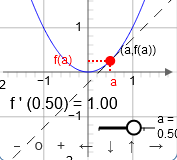
\includegraphics[width=\linewidth]{external/jsxgraph-findingslopefromtangent-exercise2b.png}
\end{sbspanel}%
\begin{sbspanel}{0.21}%

\includegraphics[width=\linewidth]{generated/qrcode/sec_basicrules1-7-6.png}
\href{http://webwork.bridgew.edu/oer/functions_at_work/sec_basicrules1-7-6.html}{Standalone}%
\par
\href{http://webwork.bridgew.edu/oer/functions_at_work/sec_basicrules1-7-6-if.html}{Embed}%
\end{sbspanel}%
\end{sidebyside}%
 The same thing is true for other power functions like \(x^3\), \(x^4\), \(x^{1/2}\), \(x^{-5}\), and so on.%
\par
In \hyperref[explore_derivativeofx2]{Exploration~{\xreffont\ref{explore_derivativeofx2}}}, we showed that when \(f(x) = x^2\), then \(f'(x) = 2x\) using the limit definition of the derivative.%
\par
In theory, you could use the limit definition of the derivative to find \(f'\) for \emph{every} power function \(f(x) = x^m\) for any constant power \(m\). Fortunately, there is a pattern in these derivatives which gives a much easier formula to remember.%
\begin{paragraphs}{The Power Rule.}{sec_basicrules1-10}%
If the exponent \(m\) is a constant number,%
\begin{equation*}
\dfrac{d}{dx}\Big[   {\color{blue} x}^{\color{red} m}= {\color{red} m} \cdot {\color{blue} x}^{{\color{red} m}-1} \Big] 
\end{equation*}
%
\par
In bracket notation, this is%
\begin{equation*}
\D{x^m} = m \cdot x^{m-1}
\end{equation*}
%
\end{paragraphs}%
\begin{exploration}{Exploration}{}{ex_usingslopefn}%
Find the slope of Let \(f(x) = x^4\).  Find the slope of \(f\) at \(x=10\), at \(x=-10\), and at \(x=0\)%
\par\smallskip%
\noindent\textbf{\blocktitlefont Solution}.\hypertarget{ex_usingslopefn-2}{}\quad{}First, we must find the slope function using the power rule%
\begin{equation*}
f'(x) = \ddx{x^4} = 4 \cdot x^{4-1} = 4 x^3
\end{equation*}
In bracket notation, this is%
\begin{equation*}
f'(x) = \D{x^4} = 4 x^{4-1} = 4x^3
\end{equation*}
%
\par
Next, we can use the  \emph{slope function} to find the slope at each given \(x\) value.%
\begin{descriptionlist}
\begin{dlimedium}{Slope at \(x=10\)}{ex_usingslopefn-2-2-3-1}%
\(\displaystyle f'(10) = 4 \cdot 10^3 = 4000 \)%
\end{dlimedium}%
\begin{dlimedium}{Slope at \(x=-10\)}{ex_usingslopefn-2-2-3-2}%
\(\displaystyle f'(-10) = 4 \cdot (-10)^3 = -4000 \)%
\end{dlimedium}%
\begin{dlimedium}{Slope at \(x=10\)}{ex_usingslopefn-2-2-3-3}%
\(\displaystyle f'(0) = 4 \cdot (0)^3 = 0 \)%
\end{dlimedium}%
\end{descriptionlist}
%
\end{exploration}%
\begin{exploration}{Exploration}{}{ex_powerruleroots}%
Let \(f(x) = \sqrt[4]{x^3} \). Find \(f'(x)\)%
\par\smallskip%
\noindent\textbf{\blocktitlefont Solution}.\hypertarget{ex_powerruleroots-2}{}\quad{}We always start by \emph{setting up the right notation}%
\begin{equation*}
f'(x) = \dfrac{d}{dx}\Big[  \sqrt[4]{x^3} \Big]
\end{equation*}
Now, we need to find a derivative rule to apply. So far, the rule we have are \(\ddx{c} = 0\), \(\ddx{mx+b} = m\), and \(\ddx{x^m} = m\cdot x^{m-1}\). None of those rules have a root in them.  Fortunately, we can use our knowledge of algebra to rewrite the \emph{original function} (without taking the derivative) to see that \(\sqrt[4]{x^3} = x^{3/4}\).  That means we can rewrite the derivative as follows%
\begin{align*}
f'(x) = \amp \dfrac{d}{dx}\Big[  \sqrt[4]{x^3} \Big] \\
=  \amp \dfrac{d}{dx}\Big[  {\color{blue} x}^{\color{red} 3/4}  \Big]
\end{align*}
Now we can use the power rule \(\dfrac{d}{dx}\Big[   {\color{blue} x}^{\color{red} m}= {\color{red} m}\cdot {\color{blue} x}^{{\color{red} m}-1} \Big] \)%
\begin{align*}
= \amp {\color{red} 3/4} \cdot {\color{blue} x}^{{\color{red} 3/4}-1} \\
= \amp \frac{3}{4} \cdot x^{-1/4} 
\end{align*}
This is an acceptable answer, but you can also rewrite if you like%
\begin{align*}
= \amp \frac{3}{4} \cdot \dfrac{1}{\sqrt[4]{x}} 
\end{align*}
%
\end{exploration}%
Square roots are particularly common, so it may be helpful to remember a specific derivative rule for square roots.%
\begin{corollary}{Corollary}{}{}{cor_powerruleroots}%
Let \(f(x) = \sqrt{x}\).  Then \(f'(x) = \frac{1}{2} x^{-1/2}\)%
\end{corollary}
\begin{proof}{Proof}{}{sec_basicrules1-15}
Recall from \emph{algebra} that roots correspond to fractional powers.  In particular\(\sqrt{x} = x^{1/2}\). Using this,%
\begin{align*}
f'(x) \amp = \ddx{x^{1/2}} \\
\amp = \frac{1}{2} x^{1/2 - 1}\\
\amp = \frac{1}{2} x^{-1/2}\qedhere
\end{align*}
%
\end{proof}
After enough practice, you should be able to use the derivative shortcut rules in this section off the top of your head.%
\par
But we will eventually learn much more complicated derivative rules, and need to apply them to more complicated functions.  To help build the skills you will need to do this, it is important to \emph{learn how to use the shortcuts using \(\dfrac{d}{dx}\Big[\dots\Big]\) or \([ \dots ]'\) notation}.%
\par
Recall from section \hyperref[sec-combining_functions]{Section~{\xreffont\ref{sec-combining_functions}}} that can break more compex functions into combinations of simpler funtions. Mathematically, we say that we build functions \emph{recursively} (layer by layer) from the inside out.%
\par
As a simple example, \(f(x) = 3x^2\) is build by taking \(x^2\), and then tripling it.  In other words, \(f(x) = triple(x^2) \).%
\par
Our derivative rules will allow us to compute derivatives from the outside in (removing one layer at a time).%
\begin{paragraphs}{Derivatives and Constant Coefficients.}{sec_basicrules1-21}%
If \(c\) is a constant number,m and \(f(x)\) is any differentiable function,%
\begin{equation*}
\dfrac{d}{dx}\Big[c\cdot f(x) \Big] = c\cdot \dfrac{d}{dx}\Big[f(x)\Big]
\end{equation*}
In bracket notation, this is%
\begin{equation*}
\D{c \cdot f(x)}  = c\cdot \D{f(x)}
\end{equation*}
%
\end{paragraphs}%
\begin{exploration}{Exploration}{}{ex_coefficientrule1}%
Let \(f(x) = 3x^2\).  Find \(\dfrac{df}{dx}\)%
\par\smallskip%
\noindent\textbf{\blocktitlefont Solution}.\hypertarget{ex_coefficientrule1-2}{}\quad{}Recall that \(\dfrac{df}{dx}\) is just another way of saying \(f'(x)\). So we can start by writing%
\begin{equation*}
f'(x) = \dfrac{d}{dx}\Big[ 3x^2 \Big]
\end{equation*}
Now, we must use one of the four rules we have so far: \(\ddx{c} = 0\), \(\ddx{mx+b} = m\), \(\ddx{x^m} = m\cdot x^{m-1}\), and \(\dfrac{d}{dx}\Big[c\cdot f(x)\Big] = c\cdot \dfrac{d}{dx}\Big[f(x)\Big]\).%
\par
The only rule that can handle the coefficient of \(3\) is the last one: \(\dfrac{d}{dx}\Big[ {\color{red}c}\cdot {\color{blue}f(x)}
\Big]
= 
{\color{red} c}\cdot \dfrac{d}{dx}\Big[\color{blue} f(x)\Big]\) That means we must interpret the problem as follows, first using the coefficient rule, and then using the power rule\textasciigrave{}%
\begin{align*}
f'(x) =  \amp \dfrac{d}{dx}\Big[{\color{red} 3}\cdot {\color{blue}x^2} \Big]\\
= \amp {\color{red} 3}  \cdot \ddx{{\color{blue}x^2} } \\
= \amp 3 \cdot 2\cdot x^{2-1}\\
= \amp 6\cdot x^{1}\\
= \amp 6\cdot x
\end{align*}
%
\par
In bracket notation, the computation is exactly the same%
\begin{equation*}
\D{3x^2} = 3\D{x^2} = 3\cdot 2 x^1 = 6x
\end{equation*}
%
\end{exploration}%
In words, the constant coefficient rule says that you can \emph{pull constant coefficients through the derivative.}%
\begin{exploration}{Exploration}{}{ex_coefficientrule2}%
Let \(f(x) = \dfrac{-2}{x}\). Find \(f'(x)\).%
\par\smallskip%
\noindent\textbf{\blocktitlefont Solution}.\hypertarget{ex_coefficientrule2-2}{}\quad{}The first step is \emph{always} to set up the problem in \(\ddx{\dots}\) or \([ \dots ]'\).%
\begin{equation*}
f'(x) = \ddxfrac{ \dfrac{-2}{x} }
\end{equation*}
Next, we look at our list of derivative rules \(\ddx{c}=0\), \(\ddx{mx+b}=m\), \(\ddx{x^m}=mx^{m-1}\), and \(\ddx{ cf(x)}=c\ddx{f(x)}\).%
\par
Unfortunately, none of these apply as written. That  means that you need to \alert{rewrite} the original function \emph{before} we can apply any rules. Here, we can use  the basic property of algebra that \(\frac{1}{x} = x^{-1}\)%
\begin{align*}
f'(x)  = \amp  \ddxfrac{ \dfrac{-2}{x} }\\
= \amp \ddx{ {\red -2} \cdot {\blue x^{-1} } }
\end{align*}
Now we can apply the derivative rule \(\ddx{ \red c} {\blue f(x) } = {\red c} \ddx{\blue f(x) }\)%
\begin{align*}
= \amp \ddx{ {\red -2} \cdot { \blue x^{-1} } }\\
= \amp {\red -2} \cdot \ddx{ {\blue x^{-1} } }
\end{align*}
Now we can use the power rule \(\ddx{ {\blue x}^{\green m} } = {\green m}\cdot {\blue x}^{{\green m}-1} \)%
\begin{align*}
= \amp { -2} \cdot \ddx{ {\blue x}^{\green -1}  }\\
= \amp { -2} \cdot {\green -1} { {\blue x}^{{\green -1} -1 }  }\\
= \amp { -2} \cdot { -1} { { x}^{-2 }  }\\
= \amp 2 { { x}^{-2 }  } = 2\dfrac{1}{x^2} = \dfrac{2}{x^2} 
\end{align*}
%
\end{exploration}%
The key idea of each of the computation above is that derivative rules attack functions from the outside in.%
\begin{paragraphs}{Derivatives of Sums and Differences.}{sec_basicrules1-26}%
Suppose that \(f(x)\) and \(g(x)\) are differentiable functions.  Then%
\begin{equation*}
\ddx{ f(x) + g(x) } = \ddx{f(x)} + \ddx{g(x)}
\end{equation*}
and%
\begin{equation*}
\ddx{f(x) - g(x) } = \ddx{f(x) } - \ddx{g(x)}
\end{equation*}
In bracket notation, this is written \(\D{f(x) + g(x)} = \D{f(x)} + \D{g(x)} \) and \(\D{f(x) - g(x)} = \D{f(x)} - \D{g(x)} \)%
\end{paragraphs}%
\begin{exploration}{Exploration}{}{ex_summdifferencerule}%
Let \(f(x) = 15x^4 + 2x^{-1} + 13\). Find \(f'(x)\), and find the slope of \(f\) at \(x=2\)%
\par\smallskip%
\noindent\textbf{\blocktitlefont Solution}.\hypertarget{ex_summdifferencerule-2}{}\quad{}As always, we need to set up%
\begin{equation*}
f'(x) = \ddx{ 15x^4 + 2x^{-1} + 13 }
\end{equation*}
and we look at our list of derivative rules \(\ddx{c}=0\), \(\ddx{mx+b}=m\), \(\ddx{x^m}=mx^{m-1}\),  \(\ddx{\frac cf(x)}=c\ddx{f(x)}\), and \(\ddx{f(x) \pm g(x)} = \ddx{f(x)} \pm \ddx{g(x)}\).%
\par
How do we decide which rule we can use? We use the order of operations to figure out the "outermost" or "weakest" operation. Following the acronym PEMDAS, subtraction and addition are the \emph{weakest} operations, so we can think of the expression as%
\begin{equation*}
f'(x) = \ddx{ \red{15x^4} + \red{2x^{-1}} + \red{13} }
\end{equation*}
Now we have the derivative of a sum, which is equal to the sum of the derivatives%
\begin{equation*}
f'(x) = \ddx{ \red{15x^4} } + \ddx{ \red{2x^{-1} } } + \ddx{\red{13}} 
\end{equation*}
Using the other, more familiar rules we can now compute%
\begin{align*}
= \amp 15\ddx{x^4} + 2\ddx{x^{-1}} + \ddx{13}\\
= \amp 15\cdot 4x^3 + 2\cdot -1 x^{-2} + 0\\
= \amp 60x^3 - 2 x^{-2} = 60 x^3 - \dfrac{2}{x^2}
\end{align*}
%
\par
To find the slope at \(x=2\), just plug 2 into the formula for \(f'(x)\).%
\begin{equation*}
f'(2) = 60 \cdot 2^3 - 2\cdot \frac{1}{2^2} = 480 - 0.5 = 479.5
\end{equation*}
%
\end{exploration}%
\begin{assemblage}{Summary}{Basic Derivative Rules.}{assemblage-basicderivatives}%
Suppose that \(f,g\) are differentiable functions of \(x\), that \(m,c\) are constant numbers.  Then%
\begin{itemize}[label=\textbullet]
\item{}\(\displaystyle \ddx{c}=0\)%
\item{}\(\ddx{m\cdot x+b}=m\) and \(\ddx{x} = 1\)%
\item{}\(\displaystyle \ddx{x^m}=m\cdot x^{m-1}\)%
\item{}\(\displaystyle \ddx{ \sqrt{x}}=\frac{1}{2}\cdot x^{-1/2}\)%
\item{}\(\displaystyle \ddx{ c\cdot f(x)}=c\cdot \ddx{f(x)}\)%
\item{}\(\displaystyle \ddx{f(x) \pm g(x)} = \ddx{f(x)} \pm \ddx{g(x)}\)%
\end{itemize}
%
\par
\alert{Danger!} The derivative rules for \(\times\) and \(\div\) are \emph{much} more complicated.  We will address those rules in a later section.%
\par
In bracket notation, these rules are written%
\begin{itemize}[label=\textbullet]
\item{}\(\displaystyle \D{c}=0\)%
\item{}\(\D{m\cdot x+b} =m\) and \([x]' = 1 \)%
\item{}\(\displaystyle \D{x^m} =m\cdot x^{m-1}\)%
\item{}\(\displaystyle \D{\sqrt{x}}=\frac{1}{2}\cdot x^{-1/2}\)%
\item{}\(\displaystyle \D{ c\cdot f(x)} =c\cdot \D{f(x)}\)%
\item{}\(\displaystyle \D{f(x) \pm g(x)}  = \D{f(x)} \pm \D{g(x)}\)%
\end{itemize}
%
\end{assemblage}
\begin{exploration}{Exploration}{}{ex_basicderivativesprofit}%
Suppose that the total profit in the scenario where you sell \(x\) items is equal to \(P(x) = -0.1x^2 + 30x - 10\). Find how fast the profit is changing when \(x=100\) items, and when \(x=200\) items.%
\par\smallskip%
\noindent\textbf{\blocktitlefont Solution}.\hypertarget{ex_basicderivativesprofit-2}{}\quad{}We will study many applications of derivatives, beginning in the next section.  For now, recall that if \(y=P(x)\) gives the \emph{total} profit in \textdollar{} in the scenario when you sell \(x\) items, then the \emph{slope of profit} \(P'(x)\) is in \textdollar{}\slash{}item, and tells you approximately how much a single additional item will change the total proift.%
\par
The first step is to find the slope function by writing%
\begin{align*}
P'(x) = \amp \ddx{ -0.1x^2 + 30x - 10 } \\
= \amp \ddx{ \red{-0.1x^2} + \red{30x} - \red{10} } \\
= \amp \ddx{\red{-0.1x^2}} + \ddx{\red{30x}} - \ddx{ \red{10} }  \\
= \amp \ddx{ \red{-0.1}\blue{x^2} } + \ddx{ \red{30} \blue{x} } - \ddx{ 10}  \\
= \amp \red{-0.1} \ddx{ \blue{x^2} } + \red{30}\ddx{ \blue{x} } - \ddx{ 10}  \\
= \amp { -0.1} \ddx{ \blue{x}^{\red{2}} } + {30}\ddx{ \blue{x} }  - \ddx{ 10}  \\
= \amp { -0.1} \cdot{ \red{2} \blue{x}^{\red{2}-1}} + {30} \cdot{ 1 } - \ddx{ 10}  \\
= \amp { -0.1} \cdot 2 \blue{x}^{1} + {30} \cdot{ 1 } - 0 \\
= \amp -0.2 x + 30  
\end{align*}
%
\par
In the scenario where you are selling \(x=100\) items, we have%
\begin{equation*}
P'(100) = -0.2(100) + 30 = 10
\end{equation*}
in \textdollar{}\slash{}item. In other words, selling an additional item (going from 100 to 101 items) will \emph{increase} total profit by approximately 10\textdollar{} for that single item.%
\par
In the scenario where you are selling \(x=100\) items, we have%
\begin{equation*}
P'(200) = -0.2(200) + 30 = -10
\end{equation*}
in \textdollar{}\slash{}item. In other words, selling an additional item (going from 200 to 201 items) will \emph{decrease} total profit by approximately 10\textdollar{} for that single item.%
\end{exploration}%
We will frequently have questions that combine \emph{several} of the strategies and concepts that we have learned in this course.  These are often called \emph{synthesis problems}.%
\par
Finding the equation for tangent lines is a classic kind of synthesis problem.%
\begin{exploration}{Exploration}{}{ex_basicderivativestangent}%
Let \(f(x) = 3x^2 - 2x + 4\). Find the equation for the line tangent to \(f(x)\) at \(x=1\).%
\par\smallskip%
\noindent\textbf{\blocktitlefont Solution}.\hypertarget{ex_basicderivativestangent-2}{}\quad{}We want to find the equation of a \emph{line}.  That means we will need to use point slope form%
\begin{equation*}
y = \red{m} (x- \red{x_1}) + \red{y_1}
\end{equation*}
Furthermore, we want the line to pass through our function at the point \(x=1\), \emph{and} we want the line to have the same slope as our function at this point.%
\par
To make sure the line passes through our curve, we set%
\begin{equation*}
x_1 = 1
\end{equation*}
and%
\begin{equation*}
y_1 = f(1) = 3\cdot 1^2 - 2\cdot 1 + 4 = 5
\end{equation*}
%
\par
To make sure the slope of this line matches the slope of the curve, we want to set%
\begin{equation*}
m = f'(1)
\end{equation*}
That means to find \(m\), we first need an equation for \(f'(x)\).%
\begin{align*}
f'(x) = \amp \ddx{ 3x^2 - 2x + 4} \\
= \amp \ddx{3x^2} - \ddx{2x} + \ddx{4} \\
= \amp 3\ddx{x^2} - 2\ddx{x} + \ddx{4} \\
= \amp 3\cdot 2x - 2\cdot 1 + 0 \\
= \amp 6x -2
\end{align*}
That means that%
\begin{equation*}
m=f'(1) = 6\cdot 1 -2 =4
\end{equation*}
Putting this all together, the equation for the line tangent to \(f\) at \(x=1 \) is%
\begin{equation*}
y = 4 (x-1) + 5
\end{equation*}
If you wanted, you could simplify this to get%
\begin{equation*}
y = 4x + 1
\end{equation*}
%
\end{exploration}%
\begin{exploration}{Exploration}{}{ex_basicderivatives_synthesis}%
Suppose that under current market conditions, your revenue is going up at 5\textdollar{}\slash{}unit and that your costs are going up at 12 \textdollar{}\slash{}unit.  How fast is your cost changing?%
\par\smallskip%
\noindent\textbf{\blocktitlefont Solution}.\hypertarget{ex_basicderivatives_synthesis-2}{}\quad{}The key concept here is to remember that%
\begin{equation*}
\text{Profit} = \text{Revenue} - \text{Cost}
\end{equation*}
Mathematically, this is%
\begin{equation*}
P(x) = R(x) - C(x)
\end{equation*}
To understand \emph{how fast profit is changing}, we must take the \emph{derivative} of profit%
\begin{equation*}
P'(x) = \ddx{ R(x) - C(x) }
\end{equation*}
Using our derivative rules,%
\begin{align*}
P'(x) = \amp \ddx{R(x) } - \ddx{C(x)} \\
= \amp R'(x) - C'(x)
\end{align*}
In the text of the problem, we are told the values of \(R'\) and \(C'\) that "under current market conditions".  In other words, we are told \(R'(x) = 5\) and \(C'(x)=12\) for whatever the "current" value of \(x\) is.  That means we can plug this information into our formula for \(P'\)%
\begin{equation*}
P'(x) = 5 - 12 = -7
\end{equation*}
Under current market conditions (for the current value of \(x\)), profit is decreasing by 7 \textdollar{}\slash{}item.%
\end{exploration}%
\begin{exploration}{Exploration}{}{ex_basicderivatives}%
\begin{enumerate}[font=\bfseries,label=(\alph*),ref=\alph*]%
\item{}Suppose that \(f(x) = 17x - 3\).  Find \(f'(x)\)%
\par\smallskip%
\noindent\textbf{\blocktitlefont Solution}.\hypertarget{ex_basicderivatives-1-2}{}\quad{}There are two ways to find this derivative.  First, note that \(f(x) = \red{ 17} x - {\blue 3} = {\red m} x + {\blue b} \) where \(m=17\) and \(b=-3\).  Using the shortcut \([mx + b]' = m\), we get%
\begin{equation*}
[mx + b]' = 17
\end{equation*}
%
\par
You can also find this derivative using the formula for derivatives of sums and differences, for constant coefficients \([m\cdot f(x)]' = m\cdot [f(x)]'\) and the formulas  \([x]' = 1\) and \([m]' = 0\) for any number \(m\).%
\begin{align*}
[ \red{ 17x}  - {\blue 3}] \amp = [17x]' - [3]' \amp \text{sum rule}\\
\amp = 17[x]' - [3]' \amp \text{coefficient rule}\\
\amp = 17\cdot 1 - 0\amp\text{basic rules}\\
\amp = 17
\end{align*}
%
\item{}Let \(f(x) = 6x^5\).  Find \(f'(x)\).%
\par\smallskip%
\noindent\textbf{\blocktitlefont Solution}.\hypertarget{ex_basicderivatives-2-2}{}\quad{}%
\begin{align*}
[6x^5]' \amp = 6\cdot [x^5]' \amp \text{coefficient rule}\\
\amp = 6\cdot 5x^4 \amp\text{power rule}\\
\amp = 30 x^4
\end{align*}
%
\item{}Let \(f(x) = 5 - 2 x^7 + 3x\).  Find \(f'(x)\)%
\par\smallskip%
\noindent\textbf{\blocktitlefont Solution}.\hypertarget{ex_basicderivatives-3-2}{}\quad{}%
\begin{align*}
[5 - 2x^5 + 3x]' \amp = [5]' - [2x^7]' + [3x]' \amp \text{sum rule}\\
\amp = [5]' - 2\cdot [x^7]' + 3\cdot[x]' \amp \text{coefficient rule}\\
\amp = [5]' - 2\cdot 7 x^6 + 3\cdot[x]' \amp\text{power rule}\\
\amp = 0 - 14 x^6 + 3\cdot 1 \amp\text{basic rules}\\
\amp = -14x^6 + 3
\end{align*}
%
\item{}Let \(f(x) = \dfrac{3}{x} + \dfrac{5}{x^2}\). Find \(f'(x)\)%
\par\smallskip%
\noindent\textbf{\blocktitlefont Solution}.\hypertarget{ex_basicderivatives-4-2}{}\quad{}Recall that \(\frac{3}{x} = 3\frac{1}{x} = 3\cdot x^{-1}\) and that \(\frac{5}{x^2} = 5\cdot\frac{1}{x^2} = 5\cdot x^{-2}\). That means we are being asked to find%
\begin{align*}
[3x^{-1} + 5x^{-2}]' \amp = [3x^{-1}]' + [5x^{-2}]' \\
\amp = 3[x^{-1}]' + 5[x^{-2}]' \\
\amp = 3(-1) x^{-1-1} + 5(-2)x^{-2-1}\\
\amp = -3 x^{-2} - 10 x^{-3}\\
\amp = \dfrac{-3}{x^2} - \dfrac{10}{x^3}
\end{align*}
%
\item{}Let \(f(x) = 3\sqrt{x} - 2 \sqrt[4]{x}\).  Find \(f'(x)\)%
\par\smallskip%
\noindent\textbf{\blocktitlefont Solution}.\hypertarget{ex_basicderivatives-5-2}{}\quad{}Recall that \(\sqrt{x} = x^{1/2}\) and that \(\sqrt[4]{x} = x^{1/4}\).  That means that we are asked to compute%
\begin{align*}
[3 x^{1/2} - 2 x^{1/4}]' \amp = [3x^{0.5} - 2x^{0.25}]'\\
\amp =  [3 x^{0.5}]' - [2 x^{0.25}]'\\
\amp = 3[x^{0.5}]' -2[x^{0.25}]' \\
\amp = 3\cdot 0.5x^{0.5-1} - 2\cdot 0.25x^{0.25-1}\\
\amp = \\
\amp = 1.5 x^{-1/2} - 0.5 x^{-3/4}\\
\amp = 1.5 \frac{1}{\sqrt{x}} - 0.5 \frac{1}{\sqrt[4]{x^3}}
\end{align*}
In most problems, you get to chose how to write your answer.  For example, you don't need to do all of the simplifications above. They are shown here to remind you of some algebra that you might need to do in other problems.%
\par
A perfectly acceptable answer to this question would be something like%
\begin{equation*}
f'(x) = 1.5 x^{-0.5} - 0.5 x^{-0.75}
\end{equation*}
%
\item{}Let \(f(x) = \dfrac{5}{\sqrt[3]{x}}\).  Find the equation for the line tangent to \(f(x)\) at \(x=1\).%
\par\smallskip%
\noindent\textbf{\blocktitlefont Solution}.\hypertarget{ex_basicderivatives-6-2}{}\quad{}Recall that the equation of the line tangent to \(f(x)\) at \(x=1\) will have the form%
\begin{equation*}
y = \red{ m} (x - \blue{ {x_1}}) + \green{{ y_1}}
\end{equation*}
where \(\blue{x_1} = \blue 1\), \(\green{y_1} = \green{ f(1)}\), and \(\red m = \red{ f'(1)}\).  We can immediately compute%
\begin{equation*}
\green{ y_1} = \green{f(1)} = \green{\dfrac{5}{\sqrt[3]{1}}} = \green{5}
\end{equation*}
To find \(\red m\), we first need an equation for \(f'(x)\).%
\begin{align*}
f'(x) \amp  = \left[ \dfrac{5}{\sqrt[3]{x}} \right]'\\
\amp = [ 5x^{-1/3}]'\\
\amp = [5 x^{-0.333\dots}]'\\
\amp = 5 [ x^{-0.333\dots}]'\\
\amp = 5 \cdot (-0.333) x^{-0.333-1}\\
\amp = 5 \cdot (-0.333) x^{-1.333}
\end{align*}
Using this, we can find that%
\begin{equation*}
\red m = f'(1) = 5\cdot (-0.333)\cdot 1^{-1.333} = -1.666\dots
\end{equation*}
Putting it all together, we get that the equation for the tangent line to \(y = f(x)\) at \(x=1\) is%
\begin{equation*}
y = \red{-1.666} (x-\blue{1}) + \green{5}
\end{equation*}
%
\end{enumerate}%
\end{exploration}%
\begin{assemblage}{Summary}{Tips for Taking Derivatives.}{sec_basicrules1-35}%
%
\begin{enumerate}
\item{}Always start by writing down%
\begin{equation*}
f'(x) = \ddx{\dots}\text{,}
\end{equation*}
filling in the original function you are given.%
\item{}Write down the derivative rules every time you use them.  To identify which rules you are \emph{allowed}, think about Order of Operations (PEMDAS).  You will be able to use the rule that goes along with the \emph{weakest} operation that you see in your expression.%
\item{}If you cannot use any derivative rule with the function as written, use algebra to rewrite the \emph{original} function.%
%
\begin{itemize}[label=\textbullet]
\item{}For example, rewriting \(\dfrac{5}{x^2} = 5\dfrac{1}{x^2} = 5x^{-2}\) can help you find the derivative of%
\begin{equation*}
\ddxfrac{\dfrac{5}{x^2}} = \ddx{5x^{-2}}
\end{equation*}
%
\item{}Rewriting \(4\cdot \sqrt[3]{x^2} = 4\cdot (x^{2/3}) \) can help you find the derivative of%
\begin{equation*}
\ddx{4\cdot \sqrt[3]{x^2}} = \ddx{4\cdot (x^{2/3})} 
\end{equation*}
%
\item{}Rewriting \(\dfrac{1}{\sqrt{x}} = \dfrac{1}{x^{1/2}}= x^{-1/2}\) can help you find the derivative of%
\begin{equation*}
\ddxfrac{\dfrac{1}{\sqrt{x}} } = \ddx{x^{-1/2} } 
\end{equation*}
%
\end{itemize}
\end{enumerate}
%
\end{assemblage}
\end{sectionptx}
%
%
\typeout{************************************************}
\typeout{Section 10.2 Derivatives of Exponentials and Logarithms}
\typeout{************************************************}
%
\begin{sectionptx}{Section}{Derivatives of Exponentials and Logarithms}{}{Derivatives of Exponentials and Logarithms}{}{}{sec-derivativesexplog}
In \hyperlink{subsec-naturalexp}{a previous section}, we have already noted that the number \emph{e\textbackslash{}approx 2.714\textbackslash{}dots} will play an important role in calculus.%
\par
More precisely, we said that \(f(x) = e^x = exp(x) = (2.714\dots)^x \) is the \emph{natural} exponential for \emph{calculus}, so we will call it the \terminology{natural exponential} function.%
\par
Just like polynomials, the \emph{slope} of the nautral exponenital function is different at different values of \(x\) \begin{sidebyside}{2}{0.075}{0.075}{0.17}%
\begin{sbspanel}{0.47}%
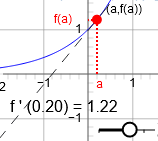
\includegraphics[width=\linewidth]{external/jsxgraph-findingslopefromtangent-exercise2c.png}
\end{sbspanel}%
\begin{sbspanel}{0.21}%

\includegraphics[width=\linewidth]{generated/qrcode/sec-derivativesexplog-4-3.png}
\href{http://webwork.bridgew.edu/oer/functions_at_work/sec-derivativesexplog-4-3.html}{Standalone}%
\par
\href{http://webwork.bridgew.edu/oer/functions_at_work/sec-derivativesexplog-4-3-if.html}{Embed}%
\end{sbspanel}%
\end{sidebyside}%
 Is there a nice \emph{formula} that gives us the slope as a function of \(x\)?  Surprisingly, the answer is yes.%
\begin{paragraphs}{The Derivative of \(e^x\).}{sec-derivativesexplog-5}%
%
\begin{equation*}
\ddx{e^x} = e^x
\end{equation*}
In bracket notation, this is%
\begin{equation*}
[e^x ]' = e^x
\end{equation*}
In other words, the \emph{slope} of any point on the curve is equal to the \emph{height} of that point on the curve.\end{paragraphs}%
\begin{exploration}{Exploration}{}{sec-derivativesexplog-6}%
Let \(f(x) = 6e^x - 2\). Find \(f'(x)\).%
\par\smallskip%
\noindent\textbf{\blocktitlefont Solution}.\hypertarget{sec-derivativesexplog-6-2}{}\quad{}%
\begin{align*}
f'(x) = \amp \ddx{ 6e^x - 2 }\\
= \amp \ddx{6e^x} - \ddx{2} \\
= \amp 6\ddx{e^x} - 0\\
= \amp 6 e^x 
\end{align*}
Note that the only new thing in this compoutation was the last step, where we used our new formula that we can replace \(\ddx{e^x}\) with \(e^x\)%
\end{exploration}%
Recall also that \(\ln(x)\), called the \terminology{natural logarithm} is the inverse of \(e^x\).  This function also has different slopes at different values of \(x\) \begin{sidebyside}{2}{0.075}{0.075}{0.17}%
\begin{sbspanel}{0.47}%
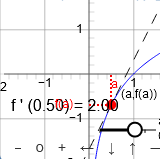
\includegraphics[width=\linewidth]{external/jsxgraph-findingslopefromtangent-exercise2d.png}
\end{sbspanel}%
\begin{sbspanel}{0.21}%

\includegraphics[width=\linewidth]{generated/qrcode/sec-derivativesexplog-7-5.png}
\href{http://webwork.bridgew.edu/oer/functions_at_work/sec-derivativesexplog-7-5.html}{Standalone}%
\par
\href{http://webwork.bridgew.edu/oer/functions_at_work/sec-derivativesexplog-7-5-if.html}{Embed}%
\end{sbspanel}%
\end{sidebyside}%
 Is there a nice \emph{formula} that gives us the slope as a function of \(x\)?  Surprisingly, the answer is \emph{also} yes.%
\begin{paragraphs}{The Derivative of \(\ln(x)\).}{sec-derivativesexplog-8}%
%
\begin{equation*}
\ddx{\ln(x) } = \dfrac{1}{x}
\end{equation*}
In bracket notation, this is%
\begin{equation*}
[ \ln(x) ]' = \dfrac{1}{x}
\end{equation*}
\end{paragraphs}%
\begin{exploration}{Exploration}{}{sec-derivativesexplog-9}%
Let \(f(x) = 3\ln(x) - x^{1/3}\). Find \(f'(x)\).%
\par\smallskip%
\noindent\textbf{\blocktitlefont Solution}.\hypertarget{sec-derivativesexplog-9-2}{}\quad{}%
\begin{align*}
f'(x) = \amp  \ddx{ 3\ln(x) - x^{1/3} } \\
= \amp \ddx{3\ln(x)} - \ddx{x^{1/3}}\\
= \amp 3\ddx{\ln(x)} - \frac{1}{3} \cdot x^{\frac{1}{3}-1} \\
= \amp 3\cdot \dfrac{1}{x} - \frac{1}{3} \cdot x^{-2/3} 
\end{align*}
%
\end{exploration}%
\begin{assemblage}{Summary}{Derivatives of Exponentials and Logarithms.}{assemblage-deriv-explog}%
%
\begin{itemize}[label=\textbullet]
\item{}\(\displaystyle \ddx{e^x} = e^x \)%
\item{}\(\displaystyle \ddx{\ln(x)} = \frac{1}{x}\)%
\end{itemize}
%
\end{assemblage}
\begin{exploration}{Exploration}{}{ex_derivatives_explog}%
\begin{enumerate}[font=\bfseries,label=(\alph*),ref=\alph*]%
\item{}Let \(f(x) = 12e^x - 2\).  Find \(f'(x)\).%
\par\smallskip%
\noindent\textbf{\blocktitlefont Solution}.\hypertarget{ex_derivatives_explog-1-2}{}\quad{}%
\begin{align*}
[12e^x - 2]'  \amp = [12e^x]' - [2]'\\
\amp = 12 [e^x]' - 0\\
\amp 12 e^x
\end{align*}
%
\item{}Let \(f(x) = 7\ln(x) + 5\).  Find \(f'(x)\)%
\par\smallskip%
\noindent\textbf{\blocktitlefont Solution}.\hypertarget{ex_derivatives_explog-2-2}{}\quad{}%
\begin{align*}
[7\ln(x) +5]'\amp = [7\ln(x)]' + [5]' \\
\amp =  7[\ln(x)]' + 0 \\
\amp = 7\cdot \frac{1}{x} \\
\amp = \frac{7}{x}
\end{align*}
%
\item{}Let \(f(x) = 3x^8 + 2e^x - 4\ln(x)\).  Find \(f'(x)\).%
\par\smallskip%
\noindent\textbf{\blocktitlefont Solution}.\hypertarget{ex_derivatives_explog-3-2}{}\quad{}%
\begin{align*}
[3x^8 + 2e^x - 4\ln(x)] \amp = [3x^8]' + [2e^x]' - [4\ln(x)]' \\
\amp  = 3[x^8]' + 2[e^x]' - 4[\ln(x)]'\\
\amp = 3\cdot 8x^7 + 2e^x - 4\cdot \frac{1}{x}\\
\amp = 24 x^7 + 2e^x - \frac{4}{x}
\end{align*}
%
\item{}Let \(f(x) = e^x + x^e \).  Find \(f'(x)\).%
\par\smallskip%
\noindent\textbf{\blocktitlefont Solution}.\hypertarget{ex_derivatives_explog-4-2}{}\quad{}This problem requires \emph{very careful reading}. The key is to remember that our \emph{only variable is \(\red x\)}.  The other characters \(e\) and \(2\) both refer to constant numbers. This is where \(\frac{d}{dx}\) notation shines, since it reminds us that the vairable is \(\red x\).%
\begin{align*}
f'(x) \amp = \ddx{ e^{\red x} + {\red x}^e} \\
\amp = \ddx{e^{\red x}} + \ddx{{\red x}^e}  
\end{align*}
Look very carefully about where the variable is in each term.  In the first term, \(x\) is in the exponent, so use the exponential rule%
\begin{equation*}
\ddx{e^{\red x}} = e^{\red x}
\end{equation*}
In the second term, \(x\) is in the base, so use the power rule with \(\blue m = \blue e = \blue 2.718\dots\)%
\begin{equation*}
\ddx{{\red x}^{\blue m} = \blue m {\red x}^{\blue m - 1}}
\end{equation*}
Putting this all together  gives the following%
\begin{align*}
f'(x) \amp = \ddx{ e^{\red x} + {\red x}^e} \\
\amp = \ddx{e^{\red x}} + \ddx{{\red x}^e}  \\
\amp = e^{\red x} + {\blue e}{\red x}^{\blue e-1}  
\end{align*}
%
\item{}Let \(f(x) = e^2 + 2^e\).  Find \(f'(x)\).%
\par\smallskip%
\noindent\textbf{\blocktitlefont Solution}.\hypertarget{ex_derivatives_explog-5-2}{}\quad{}This problem requires \emph{very careful reading}. The key is to remember that our \emph{only variable is \(\red x\)}.  The other characters \(e\) and \(2\) both refer to constant numbers. This is where \(\frac{d}{dx}\) notation shines, since it reminds us that the vairable is \(\red x\).%
\begin{align*}
f'(x) \amp = \ddx{  e^2 + 2^e} 
\end{align*}
Note that there are no \(\red x\)'s in either term.  That means we can type them into our calculator and replace them with numbers: \(e^2 = 7.389\dots\) and \(2^e = 6.580\dots\).  Putting this in and using our derivative rules gives the following%
\begin{align*}
f'(x) \amp = \ddx{  7.389 + 6.580} \\
\amp = \ddx{7.389} + \ddx{6.580} \\
\amp = 0 + 0 
\end{align*}
%
\end{enumerate}%
\end{exploration}%
\end{sectionptx}
\end{chapterptx}
 %
%
\typeout{************************************************}
\typeout{Chapter 11 Derivatives and Business}
\typeout{************************************************}
%
\begin{chapterptx}{Chapter}{Derivatives and Business}{}{Derivatives and Business}{}{}{ch_marginalcost}
\renewcommand*{\chaptername}{Chapter}
%
%
\typeout{************************************************}
\typeout{Section 11.1 Marginal Cost}
\typeout{************************************************}
%
\begin{sectionptx}{Section}{Marginal Cost}{}{Marginal Cost}{}{}{sec-marginalcost}
\begin{introduction}{}%
Derivatives provide a powerful tool for studying many concepts in economics and buisness.  In this section, we will introduce a central application in the context of cost, revenue, and profit functions. Recall that%
\begin{itemize}[label=\textbullet]
\item{}\(C(x) = \) \emph{total} cost in \textdollar{}.  For example, \(C(10)\) is the \emph{cumulative} cost of items 1-10.%
\item{}\(R(x) = \) \emph{total} revenue in \textdollar{}.  For example, \(R(10)\) is the \emph{total} revenue of items 1-10.%
\item{}\(P(x) = \) \emph{total} profit in \textdollar{}.  For example, \(P(10)\) is the \emph{total} revenue of items 1-10.%
\end{itemize}
%
\end{introduction}%
\begin{definition}{Definition}{}{defn_marginalcost}%
Let \(C(x)\) be a total cost function. The \terminology{marginal cost function} is the derivative of total cost. Furthermore,%
\begin{equation*}
C'(x) = \text{ the APPROXIMATE cost of the NEXT item in \$/item }
\end{equation*}
%
\end{definition}
\begin{exploration}{Exploration}{}{ex_marginalcost1}%
Suppose that \(C'(200) = 5\) \textdollar{}\slash{}item. Estimate the cost of the 201st item \emph{only}.%
\par\smallskip%
\noindent\textbf{\blocktitlefont Solution}.\hypertarget{ex_marginalcost1-2}{}\quad{}By \hyperref[defn_marginalcost]{Definition~{\xreffont\ref{defn_marginalcost}}}, \(C'(200) = \) the cost of the next item only.%
\par
The next item after 200 is the \emph{201st} item.  That means that The approximate cost of the 201st item is 5\textdollar{}.%
\end{exploration}%
\begin{exploration}{Exploration}{}{ex_marginalcost2}%
Suppose that \(C(x) = 120 + 5x - 0.1 x^2\)%
\begin{enumerate}[font=\bfseries,label=(\alph*),ref=\alph*]%
\item{}What is the \emph{approximate} cost of the 11th item only?%
\par\smallskip%
\noindent\textbf{\blocktitlefont Solution}.\hypertarget{ex_marginalcost2-2-2}{}\quad{}By \hyperref[defn_marginalcost]{Definition~{\xreffont\ref{defn_marginalcost}}}, when we are asked to \emph{approximate} the cost of the next item, we must find and use the marginal cost function.%
\par
To find the marginal cost function, use the derivative shortcuts%
\begin{align*}
C'(x) = \amp \ddx{ 120 + 5x - 0.1x^2 }\\
= \amp \ddx{120} + \ddx{5x} - \ddx{0.1x^2}\\
= \amp 0 + 5 - 0.1\cdot \ddx{x^2}\\
= \amp 5 - 0.1\cdot 2x\\
= \amp 5 - 0.2x
\end{align*}
%
\par
To use the marginal cost function, recall that%
\begin{equation*}
C'(x) = \text{ the APPROXIMATE cost of the NEXT item in \$/item }
\end{equation*}
We want to find the approximate cost of the 11th item. Item 11 is the item that is \emph{immediately after item 10}.%
\par
In other words, compute \(C'(10)\). That will tell us the approximate cost of the item \emph{after} 10, which is the 11th item.%
\begin{equation*}
C'(10) = 5 - 0.2\cdot 10 = 3
\end{equation*}
The 11th item will cost approximately 3\textdollar{}.%
\item{}What is the \emph{exact} cost of the 11th item only?%
\par\smallskip%
\noindent\textbf{\blocktitlefont Solution}.\hypertarget{ex_marginalcost2-3-2}{}\quad{}By definition, the total cost function \(C(x)\) gives the \emph{cumulative} cost of items \(1\) through \(x\).%
\par
In other words, \(C(11)\) tells you the \emph{cumulative} cost of items 1-11, and \(C(10)\) tells you the \emph{cumulative} cost of items 1-10.%
\par
%
\begin{align*}
\amp\amp C(11) = \amp \text{ total cost of items 1-11}  \amp \\
-\amp\Big(\amp C(10) = \amp \text{ total cost of items 1-10} \amp \Big) \\
\hline \\
\amp \amp \amp \text{cost of 11th item only} \amp 
\end{align*}
%
\par
In other words, the cost of the 11th item only is equal to%
\begin{align*}
= \amp C(11) - C(10)\\
= \amp \Big( 120 + 5\cdot 11 - 0.1(11)^2\Big) - \Big(120 + 5\cdot 10 - 0.1(10)^2\Big)   \\
= \amp 162.9 - 160\\
= \amp 2.9
\end{align*}
The exact cost of the 11th item only is \textdollar{}2.90%
\end{enumerate}%
\end{exploration}%
\begin{exploration}{Exploration}{}{ex_marginalcost3}%
You are making 100 trailers, and the total cost function is given by \(C(x) = 25,000 + 5x^3\)%
\begin{enumerate}[font=\bfseries,label=(\alph*),ref=\alph*]%
\item{}What is the \emph{exact} cost of the 100th trailer?%
\par\smallskip%
\noindent\textbf{\blocktitlefont Solution}.\hypertarget{ex_marginalcost3-2-2}{}\quad{}Recall that \(C(100) = \) total\slash{}cumulative cost of items 1 to 100.  Using the equation given,%
\begin{equation*}
C(100) = 25,000 + 5\cdot 100^3 = 5,025,000
\end{equation*}
We don't want to know the cost of \emph{all} of these items, just the last item.  To get rid of items 1-99, we compute their cost separately%
\begin{equation*}
C(99) = 25,000 + 5\cdot 99^3 = 4,876,495
\end{equation*}
Subtracting out the items we don't care about, we get%
\begin{align*}
\text{cost of 100th only} = \amp C(100) - C(99) \\
= \amp 5,025,000 - 4,876,495\\
= \amp 148,505
\end{align*}
The 100th trailer only costs exactly \textdollar{}148,505.%
\item{}What is the \emph{approximate} cost of the 100th trailer?%
\par\smallskip%
\noindent\textbf{\blocktitlefont Solution}.\hypertarget{ex_marginalcost3-3-2}{}\quad{}By \hyperref[defn_marginalcost]{Definition~{\xreffont\ref{defn_marginalcost}}}, when we are asked to \emph{approximate} the cost of the next item, we must find and use the marginal cost function.%
\par
To find the marginal cost function, use the derivative shortcuts%
\begin{align*}
C'(x) = \amp \ddx{ 25,000 + 5x^3 }\\
= \amp \ddx{25,000} + \ddx{5x^3}\\
= \amp 0 + 5\cdot \ddx{x^3}\\
= \amp 5 \cdot 3x^2\\
= \amp 15 x^2
\end{align*}
%
\par
To use the marginal cost function, recall that%
\begin{equation*}
C'(x) = \text{ the APPROXIMATE cost of the NEXT item in \$/item }
\end{equation*}
We want to find the approximate cost of the 100th item only. Item 100 is the item that is \emph{immediately after item 99}.%
\par
In other words, compute \(C'(99)\).%
\begin{equation*}
C'(99) = 15 \cdot 99^2 = 147,015
\end{equation*}
The 11th item will cost approximately \textdollar{}147,015.%
\end{enumerate}%
\end{exploration}%
The example above helps explain part of the value of using the marginal cost function, instead of always finding exact cost. Computing the exact meant talking about costs in the millions, even though the individual item's value was only in the hundreds of thousands. Even better, once we have computed the equation for marginal cost function we can quickly compare the item cost for a range of numbers of items.%
\begin{insight}{Application}{Why Derivatives Approximate the Cost of the Next Item.}{sec-marginalcost-8}%
What is the connection between derivatives and approximate item cost?%
\par
Looking at the units of measurement provides one way of understanding the connection.  If total cost \(C(x)\) is measured in dollars, and quantity \(x\) is measured in items, then%
\begin{equation*}
C'(x) = \lim_{\Delta x\rightarrow 0} = \dfrac{\Delta C}{\Delta x} \ \dfrac{\text{\$}}{\text{item}} 
\end{equation*}
In other words, because the derivative of cost has units \textdollar{}\slash{}item, it tells you approximately how many \textdollar{} an individual item will cost.%
\par
Why does the marginal cost tell us the cost of the \emph{next} item?%
\par
Remember that limits arise in business when quantities are large.  For example, suppose that \(x\) is 5000 items.%
\par
Expanding out the limit definition of slope\slash{}IROC, we get%
\begin{align*}
C'(5000) \amp = \lim_{\Delta x \rightarrow 0}\dfrac{\Delta C}{\Delta x} \\
= \amp \lim_{\Delta x \rightarrow 0} \dfrac{C_2 - C_1}{x_2 - x_1}\\
= \amp \lim_{\Delta x \rightarrow 0} \dfrac{C(5000 + \Delta x) - C(5000)}{\Delta x}
\end{align*}
Because \(x=5000\) is large, then a change of \(\Delta x=1\) more item is (relatively) small. This means that%
\begin{equation*}
C'(5000) \approx  \dfrac{C(5000 + 1) - C(5000)}{\Delta x}
\end{equation*}
simpilfying this gives%
\begin{equation*}
C'(5000) \approx  C(5001) - C(5000) 
\end{equation*}
which is equal to the 5001st item, which is the \emph{next} item after 5000.%
\end{insight}
\begin{paragraphs}{Understanding Change, AROC, and IROC.}{sec-marginalcost-9}%
We now have several tools for analyzing economic questions: \emph{change \(\Delta C\)}, average rate \(\frac{\Delta C}{\Delta x}\), and marginal cost \(C'(x) = \frac{dC}{dx}\). Always make sure you understand what the question is asking for, and know how to apply the correct tool for that question.%
%
\begin{descriptionlist}
\begin{dlimedium}{\emph{Average} and \emph{Change} look Backward}{sec-marginalcost-9-3-1}%
If you \emph{have moved} from \(x_1\) to \(x_2\) items, then you can compute the change%
\begin{equation*}
\Delta C = C_2 - C_1 
\end{equation*}
and the average rate (AROC)%
\begin{equation*}
\frac{\Delta C}{\Delta x} = \dfrac{C_2 - C_1}{x_2-x_1}
\end{equation*}
Finding the exact cost of a single item is a special case of finding the change in cost.%
\par
For example, to find the exact cost of item 105, compute \(C(105)-C(104)\).  This can be thought of as a change \(\Delta C\), or an average change \(\frac{\Delta C}{\Delta x}\) with \(\Delta x=1\)%
\par
Change and AROC are used for \emph{accounting} for changes in the \emph{past}.%
\end{dlimedium}%
\begin{dlimedium}{\emph{Marginal Cost} and \emph{Derivatives} look Foreward}{sec-marginalcost-9-3-2}%
%
\begin{align*}
C'(x) \approx \amp \text{ cost of the NEXT ITEM after} x  \\
\approx \amp \text{ cost of the } (x+1)^{st} \text{ item} 
\end{align*}
Marginal cost and derivatives are used to make \emph{decisions} about the \emph{future}%
\end{dlimedium}%
\end{descriptionlist}
\end{paragraphs}%
\par\medskip
The power of mathematics is that the same tools apply to a range of contexts.%
\begin{definition}{Definition}{}{def-marginalfunctions}%
Let \(F(x)\) be any \emph{total} or cumulatve function, such as cost, revenue, or profit. The \emph{marginal function} is%
\begin{equation*}
F'(x) = \text{ the APPROXIMATE value of the NEXT ITEM ONLY} 
\end{equation*}
%
\end{definition}
In other words, if \(R(x) = \) total revenue and \(P(x) = \) total profit, then \(R'(500) = \) approximate revenue of the next (501st) item and \(P'(500) = \) approximate revenue of the next (501st) item%
\begin{paragraphs}{Beautiful Consequence.}{sec-marginalcost-13}%
The \emph{slope of \alert{total} profit at \(x=a\) items} is approximately equal to the \emph{profit}%
\end{paragraphs}%
\end{sectionptx}
\end{chapterptx}
 %
%
\typeout{************************************************}
\typeout{Chapter 12 Product and Quotient Rule}
\typeout{************************************************}
%
\begin{chapterptx}{Chapter}{Product and Quotient Rule}{}{Product and Quotient Rule}{}{}{ch_productquotientrule}
\renewcommand*{\chaptername}{Chapter}
\begin{introduction}{}%
Previously, we have seen rules for taking derivatives of basic functions.%
\begin{assemblage}{Summary}{Basic Derivative Rules (So Far).}{assemblage-basicderivatives2}%
Suppose that \(f,g\) are differentiable functions of \(x\), that \(m,c\) are constant numbers.  Then%
\begin{itemize}[label=\textbullet]
\item{}\(\displaystyle \ddx{c}=0\)%
\item{}\(\ddx{m\cdot x+b}=m\) and \(\ddx{x} = 1\)%
\item{}\(\displaystyle \ddx{x^m}=m\cdot x^{m-1}\)%
\item{}\(\displaystyle \ddx{ c\cdot f(x)}=c\cdot \ddx{f(x)}\)%
\item{}\(\displaystyle \ddx{f(x) \pm g(x)} = \ddx{f(x)} \pm \ddx{g(x)}\)%
\item{}\(\displaystyle \ddx{ e^x } = e^x \)%
\item{}\(\displaystyle \ddx{ \ln(x) } = \frac{1}{x}\)%
\end{itemize}
%
\end{assemblage}
Previously, we noted that the derivative rules for \(\times\) and \(\div\) are \emph{much} more complicated.  We will address these rules in \hyperref[sec_productrule]{Section~{\xreffont\ref{sec_productrule}}} and \hyperref[sec_quotientrule]{Section~{\xreffont\ref{sec_quotientrule}}}.%
\end{introduction}%
%
%
\typeout{************************************************}
\typeout{Section 12.1 Derivatives of Products}
\typeout{************************************************}
%
\begin{sectionptx}{Section}{Derivatives of Products}{}{Derivatives of Products}{}{}{sec_productrule}
Remember from elementary school that the product \(h\cdot b\) is equal to the \emph{area} of the rectangle with base \(b\) and height \(h\).%
\par
Suppose now that we want the base or height to \emph{change} over time.  How does that change the area \(A = h\cdot b\) as a function of time? In other words, we want to know \(\dfrac{dA}{dt}\).%
\begin{image}{0.375}{0.25}{0.375}{}%
\resizebox{\linewidth}{!}{%
\begin{tikzpicture}
  \draw (3,0) rectangle (3.5,2);
  \draw[fill=blue,opacity=0.5] (3,0) rectangle (3.5,2);
  \draw (0,2) rectangle (3,2.5);
  \draw[fill=green,opacity=0.5] (0,2) rectangle (3,2.5);

  \draw (0,0) rectangle (3,2);
  \draw[dotted] (0,0) rectangle (3.5,2.5);

  \node[left] at (0,2.25) {$\Delta h$}; 
  \node[left] at (0,1) {$h$}; 
  \node[below] at (1.5,0) {$b$};
  \node[below] at (3.25,0) {$\Delta b$};

\end{tikzpicture}
}%
\end{image}%
Looking at the picture, there are two main parts of how the area is changing, as a result of the changing base (blue) and as a result of the changing height (green).  There is also a little area in the upper corner, but it seems negiligible compared to the other changes.%
\par
More precisely you can \emph{prove} that there are two parts to the rate of change in area%
\begin{itemize}[label=\textbullet]
\item{}\(\frac{dA}{dt}\) due to changing base is equal to \(h\cdot \frac{d}{dt}[b]\)%
\item{}\(\frac{dA}{dt}\) due to changing height is equal to \(b\cdot \frac{d}{dt}[h]\)%
\end{itemize}
Putting these together, we get the product rule:%
\begin{equation*}
\frac{d}{dt}\Big[h\cdot b\Big] = h\cdot \frac{d}{dt}\Big[b\Big] + b\cdot \frac{d}{dt}\Big[h\Big]
\end{equation*}
%
\begin{theorem}{Theorem}{The Product Rule.}{}{thm-productrule}%
Suppose that \(f(x)\) and \(g(x)\) are differentiable functions.  Then%
\begin{equation*}
\ddx{f(x)\cdot g(x)} = f\cdot \ddx{g(x)} + g(x) \cdot \ddx{f(x)}
\end{equation*}
This is eaiser to remember in bracket notation:%
\begin{equation*}
\Big[f\cdot g\Big]' = f\cdot \Big[g\Big]' + g\cdot \Big[f\Big]' 
= f\cdot g' + g\cdot f'
\end{equation*}
%
\end{theorem}
\begin{exploration}{Exploration}{}{ex_productrule1}%
Let \(f(x) = \sqrt{x} \cdot (9 + 7x) \). Find \(f'(x)\).%
\par\smallskip%
\noindent\textbf{\blocktitlefont Solution}.\hypertarget{ex_productrule1-2}{}\quad{}As always, start by setting up the derivative%
\begin{equation*}
f'(x) = \ddx{ \sqrt{x} \cdot (9 + 7x) } 
\end{equation*}
We don't have any derivative rule for square roots, but we can always rewrite \(\sqrt[m]{x^n} = x^{n/m}\).  In particular, using \(\sqrt{x} = x^{1/2}\) gives us%
\begin{equation*}
f'(x) = \ddx{ x^{1/2} \cdot (9 + 7x) } 
\end{equation*}
To apply our derivative rules, you need to use order of operations (PEMDAS) to identify the "outermost" operation. In this case, our function is the \alert{product} of \(x^{1/2}\) with \((9+7x)\).  That means we will use the \emph{product rule} \(\D{\red{f}\cdot \blue{g}} = \red{f}\cdot \D{\blue{g}} + \blue{g}\cdot \D{\red{f}}\)%
\begin{align*}
f'(x)  = \amp \ddx{ \red{x^{1/2}} \cdot \blue{(9 + 7x)} } \\
f'(x)  = \amp \red{x^{1/2}} \cdot \ddx{ \blue{(9 + 7x)} } + \blue{(9 + 7x)} \cdot \ddx{ \red{x^{1/2}} } \\
f'(x)  = \amp x^{1/2} \cdot \ddx{ (9 + 7x) } + (9 + 7x) \cdot \ddx{ x^{1/2} } \\
f'(x)  = \amp x^{1/2} \cdot \ddx{ (\red{9} + \blue{7x}) } + (9 + 7x) \cdot \ddx{ \blue{x}^{\red{1/2}} } \\
f'(x)  = \amp x^{1/2} \cdot (\ddx{\red{9}} + \ddx{\blue{7x}})  + (9 + 7x) \cdot \red{\frac{1}{2}}\cdot \blue{x}^{\red{1/2}-1}  \\
f'(x)  = \amp x^{1/2} \cdot (0 + 7)  + (9 + 7x) \cdot \frac{1}{2} \cdot x^{-1/2}  \\
f'(x)  = \amp 7\sqrt{x}  + (9 + 7x) \cdot \frac{1}{2} \cdot x^{-1/2}  \\
f'(x)  = \amp 7\sqrt{x}  + (9 + 7x) \cdot \frac{1}{2} \cdot \frac{1}{\sqrt{x}} 
\end{align*}
You could keep "simpifying" this derivative, but we might as well stop here.%
\end{exploration}%
\begin{exploration}{Exploration}{}{ex_productrule2}%
Let \(f(x) = 3x\ln(x) - 4x\). Find \(f'(x)\).%
\par\smallskip%
\noindent\textbf{\blocktitlefont Solution}.\hypertarget{ex_productrule2-2}{}\quad{}As always, start by setting up the derivative%
\begin{equation*}
f'(x) = \ddx{3x\ln(x) - 4x} 
\end{equation*}
To apply our derivative rules, you need to use order of operations (PEMDAS) to identify the "outermost" operation. In this case, our function is the \alert{sum} of \(3x\ln(x)\) and  \(-4x\).  That means we will use the \emph{sum rule} \(\D{\red{f} + \blue{g}} = \D{\red{f}} + \D{\blue{g}}\)%
\begin{align*}
f'(x) = \amp \ddx{ \red{3x\ln(x)} - \blue{4x}  } \\
= \amp \ddx{ \red{3x\ln(x)} } - \ddx{\blue{4x}  } \\
= \amp \ddx{ 3x\ln(x) } - \ddx{ 4x  } 
\end{align*}
Now we have \emph{two separate} derivatives to compute: \(\ddx{ 3x\ln(x) } \) and \(\ddx{4x}\). The second derivative is easy: \(\ddx{4x}=4\).%
\begin{align*}
f'(x) = \amp \ddx{ 3x\ln(x) } - 4 \\
= \amp \ddx{ \red{3x}\cdot \blue{\ln(x)} } - 4 
\end{align*}
For the remaining derivative, we need to use PEMDAS to identify the "outermost" operation, which is a product, so we will use the product rule \(\D{\red{f}\cdot \blue{g}} = \red{f}\cdot \D{\blue{g}} + \blue{g}\cdot \D{\red{f}}\)%
\begin{align*}
f'(x) = \amp \ddx{ \red{3x}\cdot \blue{\ln(x)} } - 4 \\
= \amp \red{3x}\cdot \ddx{\blue{\ln(x)} } + \blue{\ln(x)}\cdot \ddx{\red{3x}} - 4 \\
= \amp 3x\cdot \ddx{ \ln(x) } + \ln(x) \cdot \ddx{ 3x } - 4 
\end{align*}
The remaining derivatives are basic rules: \(\ddx{\ln(x)} = 1/x\) and \(\ddx{cx} = c\).%
\begin{align*}
f'(x) = \amp 3x\cdot \frac{1}{x} + \ln(x) \cdot 3 - 4 \\
= \amp \frac{3x}{x} + 3\ln(x) - 4 \\
= \amp 3 + 3\ln(x) - 4 \\
= \amp 3\ln(x) - 1 
\end{align*}
%
\end{exploration}%
\begin{exploration}{Exploration}{}{ex_productrule3}%
Let \(f(x) = 5x^3\, e^x\,\ln(x)\).  Find \(f'(x)\).%
\par\smallskip%
\noindent\textbf{\blocktitlefont Solution}.\hypertarget{ex_productrule3-2}{}\quad{}This problem requires several steps.  First, begin by setting up the question%
\begin{align*}
f'(x) = \amp \D{5x^3\cdot e^x\cdot\ln(x)}  
\end{align*}
We want to take the derivative of a product, so we must use the product rule \(\D{\red{f}\cdot\blue{g}} = \red{f}\cdot\D{\blue{g}} + \blue{g}\cdot\D{\red{f}}\).  The problem is that  here are only \emph{two} functions in our formula, but there are multiplied terms in our definition of \(f\).  Fortunately, because of the ``associativity'' of multiplication \(a\cdot b\cdot c = (a\cdot b)\cdot c = a\cdot (b\cdot c)\), so we can group the terms any way we like.%
\begin{align*}
f'(x) = \amp \D{\red{(5x^3\, e^x)}\cdot \blue{\ln(x)}}  \\
= \amp \red{(5x^3\, e^x)}\cdot \D{\blue{\ln(x)}}  +  \blue{\ln(x)}\D{\red{(5x^3\, e^x)} } 
\end{align*}
Now we have two derivatives remaining: a simple derivative \(\D{{\ln(x)}} = \frac{1}{x}\) and a product rule \(\D{{(5x^3\cdot e^x)} } = 5x^3 \cdot \D{e^x} + e^x\cdot \D{5x^3} = 5x^3 e^x + e^x\, 15x^2\).  Putting it all together we get%
\begin{align*}
\phantom{f'(x)} = \amp {(5x^3\, e^x)}\cdot \frac{1}{x}  +  {\ln(x)}\cdot \Big( 5x^3 e^x + e^x\, 15x^2 \Big) \\
\phantom{f'(x)} = \amp 5x^3\, e^x \,\frac{1}{x}  +   5x^3\, e^x\, \ln(x) + 15x^2\,e^x\,  \ln(x) 
\end{align*}
%
\end{exploration}%
Any time a product is changing, the product rule comes into play. In business, products play an important role in the study of revenue and profit, since%
\begin{equation*}
\text{Revenue } = \text{ price }\cdot \text{ quantity } = p\cdot q
\end{equation*}
Previously, we have only looked at the impact of changing quanitity. But in \emph{real economies}, things like marketing can increase the quanitity sold over time \emph{without} decreasing the price.%
\begin{exploration}{Exploration}{}{ex_productrule4}%
Thanks to a word of mouth marketing campaign, business is booming.  Suppose that%
\begin{align*}
\text{quantity on day }t =\amp q(t) = 0.4e^t \\
\text{price on day }t =\amp p(t) = t^2   
\end{align*}
How fast is Revenue changing on day 3?%
\par\smallskip%
\noindent\textbf{\blocktitlefont Solution}.\hypertarget{ex_productrule4-2}{}\quad{}Before we can find any rates of change with respect to time, we first need to know what the revenue function is as a function of \(t\).  Using the formula%
\begin{equation*}
\text{Revenue } = \text{ price }\cdot \text{ quantity }
\end{equation*}
we have%
\begin{equation*}
R(t) = p(t) \cdot q(t) = t^2\cdot 0.4e^t
\end{equation*}
Now, we can find the derivative with respect to t%
\begin{align*}
R'(t) = \amp \ddt{ t^2\cdot 0.4e^t } \\
= \amp \ddt{ \red{t^2}\cdot \blue{0.4e^t} } \\
= \amp \red{t^2}\cdot\ddt{  \blue{0.4e^t} } + \blue{0.4e^t}\cdot \ddt{ \red{t^2} }  \\
= \amp t^2\cdot\ddt{  \red{0.4}\blue{e^t} } + 0.4e^t \cdot \ddt{ \blue{t}^{\red{2}} }  
\end{align*}
For the first derivative, we have a constant coefficent times a function, so we can use the rule \(\ddx{\red{c}\blue{f(x)}} = \red{c} \ddx{\blue{f(x)} }\). For the second derivative, we can use the power rule \(\ddx{\blue{x}^{\red{m}}} = \red{m} \blue{x}^{\red{m}-1}\)%
\begin{align*}
R'(t) = \amp t^2\cdot \red{0.4}\ddt{ \blue{e^t} } + 0.4e^t \cdot \red{2} \blue{t}^{\red{2}-1}   \\
R'(t) = \amp t^2\cdot 0.4 \ddt{ e^t } + 0.4e^t \cdot 2 t^{1}   \\
R'(t) = \amp t^2\cdot 0.4 e^t  + 0.4e^t \cdot 2 t   \\
R'(t) = \amp 0.4 t^2 e^t  + 0.8 t e^t   
\end{align*}
On day \(3\), the rate of change of revenue is%
\begin{equation*}
R'(3) = 0.4 \cdot 3^2 e^3  + 0.8\cdot  3 \cdot e^3 = 192.82
\end{equation*}
On the third day, the price is going up approximately 192.82 \textdollar{}\slash{}day.%
\end{exploration}%
In general, if price \(p(t)\) and quanity \(q(t)\) are both functions of \(t\), then because the revenue function is%
\begin{equation*}
R = q\cdot p
\end{equation*}
then the rate of change of revenue is%
\begin{equation*}
\frac{dR}{dt} = q\cdot \frac{dp}{dt} + p \cdot \frac{dq}{dt}
\end{equation*}
In other words, the rate of revenue change has two parts: the change in \(R\) due to changing price (the first term), and the change in \(R\) due to changing quanity (the second term).%
\end{sectionptx}
%
%
\typeout{************************************************}
\typeout{Section 12.2 Derivatives of Fractions}
\typeout{************************************************}
%
\begin{sectionptx}{Section}{Derivatives of Fractions}{}{Derivatives of Fractions}{}{}{sec_quotientrule}
There is also a special rule for derivatives of fractions. Another name for a fraction is a \emph{quotient}, so this is often called the \terminology{quotient rule}.%
\begin{theorem}{Theorem}{}{}{thm-quotientrule}%
Suppose that \(f(x)\) and \(g(x)\) are differentiable functions.  Then%
\begin{equation*}
\ddxfrac{\dfrac{f(x)}{g(x)}} = \dfrac{g(x) \cdot \ddx{f(x)} - f(x) \cdot \ddx{g(x)} }{\Big(g(x)\Big)^2}
\end{equation*}
It is often easier to memorize this formula in an abbreviated form:%
\begin{itemize}[label=\textbullet]
\item{}\(\displaystyle \left[\dfrac{t}{b}\right]' = \dfrac{b\cdot t' - t\cdot b'}{(b)^2} \)%
\item{}\(\displaystyle \left[\dfrac{\text{hi}}{\text{lo}} \right] = \dfrac{\text{lo }D\text{ hi} - \text{hi }D\text{ lo} }{(\text{lo})^2}\)%
\end{itemize}
%
\end{theorem}
\begin{exploration}{Exploration}{}{ex_quotientrule1}%
Let \(f(x) = \dfrac{e^x}{x}\). Find \(f'(10)\).%
\par\smallskip%
\noindent\textbf{\blocktitlefont Solution}.\hypertarget{ex_quotientrule1-2}{}\quad{}%
\begin{equation*}
f'(x) = \ddxfrac{  \dfrac{e^x}{x}  }
\end{equation*}
To apply our derivative rules, you need to use order of operations (PEMDAS) to identify the "outermost" operation. In this case, our function is the \alert{fraction} of \(e^x\) and  \(xx\).  That means we will use the \emph{quotient rule} \(\left[\dfrac{\red{t}}{\blue{b}}\right]' = \dfrac{\blue{b}\cdot \red{t}' - \red{t}\cdot \blue{b}'}{(\blue{b})^2}\)%
\begin{align*}
f'(x) = \amp \ddxfrac{  \dfrac{\red{e^x}}{\blue{x}}  }\\
= \amp \dfrac{\blue{x}\cdot \ddx{\red{e^x}} - \red{e^x} \ddx{\blue{x}}}{(\blue{x})^2}\\
= \amp \dfrac{ x\cdot \ddx{ e^x } - e^x \ddx{ x }}{(x)^2}\\
= \amp \dfrac{ x\cdot e^x - e^x \cdot 1}{(x)^2}\\
= \amp \dfrac{ x\cdot e^x - e^x }{(x)^2}
\end{align*}
At \(x=10\),%
\begin{equation*}
f'(10) = \dfrac{ 10\cdot e^{10} - e^{10} }{(10)^2} = 1982.38
\end{equation*}
%
\end{exploration}%
You can "show your work" in several ways. We have already seen the \(\ddx{\dots}\) strategy. This strategy is good because it is very robust, and almost always works. Unfortunately, this strategy also uses a \emph{lot} of symbols.%
\par
An alternative technique makes a much greater use of scrap work.  We will illustrate this strategy using the following exercise.%
\begin{exploration}{Exploration}{}{ex_quotientrule2}%
Let \(f(x) = \dfrac{x^2 + x + 1}{x^2 -1 }\). Find \(\frac{df}{dx}\).%
\par\smallskip%
\noindent\textbf{\blocktitlefont Solution}.\hypertarget{ex_quotientrule2-2}{}\quad{}As always,  start by setting up the derivative.%
\begin{equation*}
f'(x) = \ddx{ \dfrac{ \red{x^2 + x + 1} }{ \blue{x^2 -1} } }
\end{equation*}
The outermost operation is a fraction, so we must use the quotient rule \(\left[\dfrac{\red{t}}{\blue{b}}\right]' = \dfrac{\blue{b}\cdot \red{t'} - \red{t}\cdot \blue{b'}}{(\blue{b})^2}\) with%
\begin{equation*}
t = x^2 + x + 1
\end{equation*}
and%
\begin{equation*}
b = x^2 - 1\text{.}
\end{equation*}
For the quotient rule, we need to subsitute expressions for \(t\), \(b\), \(t'\), and \(b'\). We already have expressions for \(t\) and \(b\).  We next do some "scrap work" to find \(t'\) and \(b'\)%
\begin{align*}
t' = \amp \ddx{x^2 + x + 1} \\
= \amp \ddx{x^2} + \ddx{x} + \ddx{1}\\
t'= \amp 2x+1+ 0\\
t'= \amp 2x+1
\end{align*}
Similarly, we can compute%
\begin{align*}
b' = \amp \ddx{x^2 - 1} \\
= \amp \ddx{x^2} - \ddx{1}\\
b'= \amp 2x - 0\\
b'= \amp 2x
\end{align*}
We now can go back to our original question, and apply the quotient rule%
\begin{align*}
f'(x) = \amp \ddx{ \dfrac{ \red{x^2 + x + 1} }{ \blue{x^2 -1} } }\\
=  \amp \dfrac{\blue{b}\cdot \red{t'} - \red{t}\cdot \blue{b'}}{(\blue{b})^2}\\
= \amp \dfrac{\blue{(x^2 - 1)}\cdot \red{(2x+1)} - \red{(x^2 + x + 1)}\cdot \blue{2x}}{(\blue{x^2 - 1})^2} 
\end{align*}
%
\end{exploration}%
\begin{exploration}{Exploration}{}{ex_quotientrule3}%
Let \(f(x) = \dfrac{x^2}{\ln(x)}\). Find \(f'(x)\).%
\par\smallskip%
\noindent\textbf{\blocktitlefont Solution}.\hypertarget{ex_quotientrule3-2}{}\quad{}%
\begin{equation*}
f'(x) = \ddx{ \dfrac{ \red{x^2} }{ \blue{\ln(x)}  } }
\end{equation*}
We must use the quotient rule \(\left[\dfrac{\red{t}}{\blue{b}}\right]' = \dfrac{\blue{b}\cdot \red{t'} - \red{t}\cdot \blue{b'}}{(\blue{b})^2}\)%
\begin{align*}
f'(x) =  \amp \ddx{ \dfrac{ \red{x^2} }{ \blue{\ln(x)}  } } \\
= \amp  \dfrac{ \blue{\ln(x)}\cdot \ddx{\red{x^2}} - \red{x^2}\cdot \ddx{\blue{\ln(x)}} }{ \blue{\Big(\ln(x)\Big)^2}  } \\
= \amp \dfrac{ \ln(x) \cdot 2x - x^2\cdot \frac{1}{x} }{ \Big(\ln(x)\Big)^2 }\\
= \amp \dfrac{ 2x\ln(x)- x }{ \Big(\ln(x)\Big)^2 }
\end{align*}
%
\end{exploration}%
\begin{exploration}{Exploration}{}{ex_quotientrule4}%
Let \(y= \dfrac{x\ln(x)}{e^x}\). Find \(\dfrac{dy}{dx}\)%
\par\smallskip%
\noindent\textbf{\blocktitlefont Solution}.\hypertarget{ex_quotientrule4-2}{}\quad{}%
\begin{equation*}
f'(x) = \ddxfrac{ \dfrac{ \red{ x\ln(x)} }{ \blue{e^x} } }
\end{equation*}
The most important part of any derivative is to find the "outermost" operation. Here, we have a \emph{fraction} where the numerator is \(x\ln(x)\) and the denominator is \(e^x\). We must use the quotient rule. \(\left[\dfrac{\red{t}}{\blue{b}}\right]' = \dfrac{\blue{b}\cdot \red{t'} - \red{t}\cdot \blue{b'}}{(\blue{b})^2}\)%
\begin{align*}
f'(x) = \amp \dfrac{\blue{e^x} \ddx{\red{x\ln(x)}} - \red{x\ln(x)}\ddx{\blue{e^x}}}{(\blue{e^x})^2}
\end{align*}
There are two derivatives in the expression above.  The second expression is straightforward: \(\ddx{e^x}=e^x\).  The first derivative is more complicated is a product, so will require the product rule \(\ddx{\red{x} \blue{\ln(x)}} = \red{x}\ddx{\blue{\ln(x)}} + \blue{\ln(x)}\ddx{\red{x}} = x\frac{1}{x} + \ln(x)\cdot 1 = \green{1 + \ln(x)}\)%
\begin{align*}
f'(x) = \amp \dfrac{ e^x  \ddx{ \red{x}\cdot \blue{\ln(x)} }  -  x\ln(x) e^x }{( e^x )^2}\\
= \amp \dfrac{ e^x  \green{\Big(1 + \ln(x)\Big)}  -  x\ln(x) e^x }{( e^x )^2}
\end{align*}
%
\end{exploration}%
\end{sectionptx}
\end{chapterptx}
 %
%
\typeout{************************************************}
\typeout{Chapter 13 The Chain Rule}
\typeout{************************************************}
%
\begin{chapterptx}{Chapter}{The Chain Rule}{}{The Chain Rule}{}{}{ch_chainrule}
\renewcommand*{\chaptername}{Chapter}
\begin{introduction}{}%
So far, we have seen rules for sums, products, and quotients \begin{assemblage}{Summary}{Basic Derivative Rules (So Far).}{assemblage-basicderivatives3}%
Suppose that \(f,g\) are differentiable functions of \(x\), that \(m,c\) are constant numbers.  Then%
\begin{itemize}[label=\textbullet]
\item{}\(\displaystyle \D{c}=0\)%
\item{}\(\D{m\cdot x+b}=m\) and \(\D{x} = 1\)%
\item{}\(\displaystyle \D{x^m}=m\cdot x^{m-1}\)%
\item{}\(\displaystyle \D{ c\cdot f(x)}=c\cdot \D{f(x)}\)%
\item{}\(\displaystyle \D{f(x) \pm g(x)} = \D{f(x)} \pm \D{g(x)}\)%
\item{}\(\displaystyle \D{ e^x } = e^x \)%
\item{}\(\displaystyle \D{ \ln(x) } = \frac{1}{x}\)%
\item{}\(\displaystyle \Big[f\cdot g\Big]' = f\cdot \Big[g\Big]' + g\cdot \Big[f\Big]' = f\cdot g' + g\cdot f' \)%
\item{}\(\displaystyle \left[\dfrac{t}{b}\right]' = \dfrac{b\cdot t' - t\cdot b'}{(b)^2} \)%
\end{itemize}
%
\end{assemblage}
%
\par
But what happens if you have a function \emph{inside} of another function?%
\par
For example, in Excel you will often see an expression like%
\begin{equation*}
\ln\Big( x^2 \Big)
\end{equation*}
Here, the function \(\red{x^2}\) is \emph{inside} the function \(\ln\Big(\red{u}\Big)\). In this case, we call%
\begin{itemize}[label=\textbullet]
\item{}the inside function \(\red{g(x)} = \red{x^2}\) the \terminology{argument} or \terminology{inner function}%
\item{}the outside function \(f(\red{u}) = \ln\Big(\red{u}\Big)\) is the \terminology{outer function}%
\item{}the original function \(f(\red{g(x)}) = \ln\Big( \red{x^2} \Big)\) is the \terminology{composition} of the outside function and the argument.%
\end{itemize}
%
\par
In this chapter, we will introduce one final rule (or set of rules) that will let us compute derivatives of compositions of functions.%
\end{introduction}%
%
%
\typeout{************************************************}
\typeout{Section 13.1 The Generalized Power Rule}
\typeout{************************************************}
%
\begin{sectionptx}{Section}{The Generalized Power Rule}{}{The Generalized Power Rule}{}{}{sec_generalizedpowerrule}
Compositions where the outside function is a power is the simplest case to work with.%
\begin{inlineexercise}{Checkpoint}{}{ex_generalizedpower_decomposing}%
Let \(h(x) = (3x+2)^2\). Write this function in the form \(f\Big(g(x)\Big)\)%
\par\smallskip%
\noindent\textbf{\blocktitlefont Solution}.\hypertarget{ex_generalizedpower_decomposing-2}{}\quad{}The easiest way to interpret compositions is to try to \emph{circle the inside function}.%
\begin{equation*}
h(x) = \Big( \red{\framebox{3x+2}} \Big)^2
\end{equation*}
%
\begin{itemize}[label=\textbullet]
\item{}The \terminology{argument} is the circled inside term \(\red{g(x)} = \color{red} \framebox{3x+2}\).%
\item{}To find the \terminology{outside function}, replace the circled box with the letter \(u\).%
\begin{align*}
h(u) = \amp \Big( \red{\framebox{3x+2}} \Big)^2  \\
= \amp \Big( \red{\framebox{u}} \Big)^2  \\
h(u) = \amp \red{u}^2
\end{align*}
%
\end{itemize}
If \(f(u) = u^2\) and \(g(x) = 3x+2\), then%
\begin{equation*}
f\Big(g(x)\Big) = f\Big(3x+2\Big) = (3x+2)^2
\end{equation*}
as desired.%
\end{inlineexercise}%
In very simple cases, we can compute the derivative of a composition with the rules we already have.%
\begin{inlineexercise}{Checkpoint}{}{ex_powerrule-nopower}%
Let \(f(x) = (3x+2)^2\).  Find \(f'(x)\) using only the rules from the previous sections.%
\par\smallskip%
\noindent\textbf{\blocktitlefont Solution}.\hypertarget{ex_powerrule-nopower-2}{}\quad{}%
\begin{equation*}
f'(x) = \ddx{ \Big(3x+2\Big)^2 } 
\end{equation*}
No rule applies, but we can rewrite the function using algebra first.%
\begin{align*}
f'(x) = \amp  \ddx{ \Big(3x+2\Big)^2 } \\
= \amp \ddx{  \Big(3x+2\Big)\cdot  \Big(3x+2\Big) }\\
= \amp \ddx{  9x^2 + 12x + 4 }\\
= \amp \ddx{9x^2} + \ddx{12x} + \ddx{4} \\
= \amp 9\ddx{x^2} + 12 + 0 \\
= \amp 9\cdot 2x + 12  \\
= \amp 18x + 12  
\end{align*}
On the face of it, there is no clear connection between the equations for \(f(x)\) and \(f'(x)\). We need a new shortcut.%
\end{inlineexercise}%
\begin{theorem}{Theorem}{The Generalized Power Rule.}{}{thm-generalizedpowerrule}%
Suppose that \(g(x)\) is a differentiable function, and that \(m\) is a constant number.%
\begin{equation*}
\ddx{ \Big( g(x) \Big)^m} = m\cdot \Big( g(x) \Big)^{m-1} \cdot \ddx{g(x)} 
\end{equation*}
In other words, if you have a composition \(h(x) = \Big(g(x)\Big)^m\), the derivative is the same thing as following the power rule and multiplying by the derivative of the argument.%
\par
In bracket notation, this rule is written%
\begin{equation*}
\D{ \Big(g(x)\Big)^m } = m\cdot \Big(g(x)\Big)^{m-1}\cdot g'(x)
\end{equation*}
%
\end{theorem}
\begin{inlineexercise}{Checkpoint}{}{ex_powerrule1}%
Let \(h(x) = (3x+2)^2\) as before.  Find \(h'(x)\) using the generalized power rule.%
\par\smallskip%
\noindent\textbf{\blocktitlefont Solution}.\hypertarget{ex_powerrule1-2}{}\quad{}As always, start by writing%
\begin{equation*}
h'(x) = \ddx{ \blue{(\red{3x+2})^2} } 
\end{equation*}
As in \hyperref[ex_generalizedpower_decomposing]{Checkpoint~{\xreffont\ref{ex_generalizedpower_decomposing}}}, this is a composition with argument \(g(x) = 3x+2\) and outside function \(f(u) = u^2\). We must use the generalized power rule \(\ddx{ \blue{ \Big( \red{g(x)} \Big)^m}} = \blue{ m\cdot \Big( \red{g(x)} \Big)^{m-1} } \cdot \ddx{\red{g(x)}} \)%
\begin{align*}
h'(x) = \amp \ddx{ \blue{ ( \red{3x+2} )^2 } }\\
= \amp \ddx{\blue{ ( \red{g(x)} )^2 } } \\
= \amp \blue{ 2\cdot ( \red{g(x)} )^1 }\cdot \ddx{ \red{g(x)} }\\
= \amp \blue{2\cdot ( \red{3x+2} ) }\cdot \ddx{ \red{3x+2} }\\
= \amp 2\cdot (3x+2) \cdot (3+0)\\
= \amp 18x+12
\end{align*}
%
\end{inlineexercise}%
\begin{inlineexercise}{Checkpoint}{}{ex_powerrule2}%
Let \(h = \Big(3-\ln(x)\Big)^{10}\). Find \(\frac{dh}{dx}\).%
\par\smallskip%
\noindent\textbf{\blocktitlefont Solution}.\hypertarget{ex_powerrule2-2}{}\quad{}%
\begin{equation*}
\frac{dh}{dx} = \ddx{ \blue{ \Big( \red{3-\ln(x)}\Big)^{10} } } 
\end{equation*}
This is a composition of two functions, with the inside function (argument) \(\red{g(x) = 3-\ln(x)} \) and outside function \(\blue{f(u)} = \blue {u^{10}}\)%
\begin{align*}
\frac{dh}{dx} =  \amp \ddx{ \blue{ \Big( \red{3-\ln(x)}\Big)^{10} } } \\
= \amp \ddx{\blue{ ( \red{g(x)} )^{10} } } \\
= \amp \blue{ 10\cdot ( \red{g(x)} )^9 }\cdot \ddx{ \red{g(x)} }\\
= \amp \blue{10\cdot ( \red{3-\ln(x)} )^9 }\cdot \ddx{ \red{3-\ln(x)} }\\
= \amp 10\cdot \Big(3-\ln(x)\Big)^9\cdot \Big( 0 - \frac{1}{x}\Big)\\
= \amp -10 \Big(3-\ln(x)\Big)^9\cdot \frac{1}{x}
\end{align*}
%
\end{inlineexercise}%
\begin{inlineexercise}{Checkpoint}{}{ex_powerrule3}%
Let \(y = \dfrac{1}{x^2-3x}\).  Find \(\frac{dy}{dx}\).%
\par\smallskip%
\noindent\textbf{\blocktitlefont Solution}.\hypertarget{ex_powerrule3-2}{}\quad{}%
\begin{equation*}
\ddxfrac{\frac{dy}{dx}} = \ddxfrac{  \dfrac{1}{x^2-3x} }
\end{equation*}
You can compute this derivative using the quotient rule, as in \hyperref[sec_quotientrule]{Section~{\xreffont\ref{sec_quotientrule}}}. You can also rewrite this as a power, and use the generalized power rule.%
\begin{equation*}
\ddxfrac{\frac{dy}{dx}} = \ddxfrac{  \Big(x^2-3x\Big)^{-1} }
\end{equation*}
You are now taking the derivative of a composition with argument \(\red{g(x)} = \red{x^2-3x}\) and outside function \(\blue{f(u)} = \blue{u^{-1}} \).%
\begin{align*}
\frac{dy}{dx} = \amp \ddxfrac{ \blue{ \Big(\red{x^2-3x}\Big)^{-1} } } \\
= \amp \ddx{\blue{ ( \red{g(x)} )^{-1} } } \\
= \amp \blue{ -1\cdot ( \red{g(x)} )^{-1-1} }\cdot \ddx{ \red{g(x)} }\\
= \amp \blue{ -1\cdot ( \red{x^2-3x} )^{-2} }\cdot \ddx{ \red{x^2-3x} }\\
= \amp  -1\cdot ( x^2-3x )^{-2} \cdot \Big(2x-3\Big) \\
= \amp  -1\cdot \dfrac{1}{( x^2-3x )^{2}} \cdot \Big(2x-3\Big) 
\end{align*}
%
\end{inlineexercise}%
\begin{inlineexercise}{Checkpoint}{}{ex_powerrule4}%
Use the product and chain rules to derive equation for the quotient rule.%
\par\smallskip%
\noindent\textbf{\blocktitlefont Solution}.\hypertarget{ex_powerrule4-2}{}\quad{}Suppose that  \(f(x)\) and \(g(x)\) are differentiable functions.  We wish to compute%
\begin{equation*}
\ddx{ \dfrac{f(x)}{g(x)} } 
\end{equation*}
To use the product and generalized power rule, we can get rid of the fraction by using an exponent of \(-1\).%
\begin{equation*}
\ddx{ \dfrac{f(x)}{g(x)} }  = \ddx{ \red{f(x)}\cdot \blue{ \Big(g(x)\Big)^{-1}} } 
\end{equation*}
Using the product rule, we get%
\begin{equation*}
\ddx{ \dfrac{f(x)}{g(x)} }  = \red{f(x)}\cdot \ddx{ \blue{ \Big(g(x)\Big)^{-1}} } +  \blue{ \Big(g(x)\Big)^{-1}}\cdot \ddx{ \red{f(x)}  } 
\end{equation*}
There are two \(\ddx{\dots}\) that remain.  The second one is simply notation: \(\ddx{f(x)} = f'(x)\). The first requires the chain rule%
\begin{align*}
\ddx{ \blue{ \Big( \red{g(x)} \Big)^{-1} }  } = \amp \blue{-1 \Big(\red{g(x)} \Big)^{-1-1}} \cdot \ddx{\red{g(x)}} \\
= \amp -1 \Big(g(x)\Big)^{-2}\cdot g'(x)
\end{align*}
Putting this back into the broader derivative%
\begin{align*}
\ddx{ \dfrac{f(x)}{g(x)} }  = \amp f(x) \cdot -1 \Big(g(x))^{-2}\cdot g'(x) +   \Big(g(x)\Big)^{-1}\cdot  f'(x)   \\
=  \amp \frac{-f(x)\cdot g'(x)}{\Big(g(x)\Big)^2} + \frac{f'(x)}{g(x)} 
\end{align*}
To combine these fractions, we need a common denominator%
\begin{align*}
=  \amp \frac{-f(x)\cdot g'(x)}{\Big(g(x)\Big)^2} + \frac{f'(x)\cdot g(x)}{\Big(g(x)\Big)^2} \\
=  \amp \frac{-f(x)\cdot g'(x) + f'(x)\cdot g(x)}{\Big(g(x)\Big)^2} 
\end{align*}
Rearranging the top gives%
\begin{align*}
=  \amp \frac{ g(x)\cdot f'(x) - f(x)\cdot g'(x) }{\Big(g(x)\Big)^2} 
\end{align*}
This is exactly the quotient rule from \hyperref[thm-quotientrule]{Theorem~{\xreffont\ref{thm-quotientrule}}}.%
\end{inlineexercise}%
\begin{inlineexercise}{Checkpoint}{}{ex_powerrule5}%
Let \(f(x) = \sqrt{5-3x+x^5} + 10 \).  Find \(f'(x)\)%
\par\smallskip%
\noindent\textbf{\blocktitlefont Solution}.\hypertarget{ex_powerrule5-2}{}\quad{}Recall that \(\sqrt{g(x)} = \Big(g(x)\Big)^{1/2} =\Big(g(x)\Big)^{0.5}  \).  That means we can rephrase the question given as follows.%
\begin{align*}
f'(x) \amp = \D{ (5-3x+x^5)^{0.5} + 10 } \\
\amp =  \D{ (5-3x+x^5)^{0.5} }  + \D{ 10 } \amp \text{sum rule}\\
\amp =  \D{ \blue{(\red{5-3x+x^5})^{0.5}} }  + 0 \amp \text{constant  rule} \\
\amp = \blue{0.5 \Big(\red{5-3x+x^5}\Big)^{0.5-1}}\cdot\D{\red{5-3x+x^5}} \amp \text{chain rule} \\
\amp = 0.5 \Big( 5-3x+x^5 \Big)^{-0.5}\cdot\Big( 0-3+5x^4\Big) 
\end{align*}
Note that both sets of parentheses in the last term are required for a correct answer.%
\end{inlineexercise}%
Recall that for root functions, we have an optional derivative shortcut \(\ddx{\sqrt{x}}=\frac{1}{2}x^{-1/2}\).  Combined with the generalized power rule, this gives an optional shortcut.%
\begin{corollary}{Corollary}{}{}{cor_generalizedroot}%
Let \(f(x) = \sqrt{g(x)}\). Then \(f'(x) = \frac{1}{2} \Big(g(x)\Big)^{-1/2}\cdot g'(x)\)%
\end{corollary}
\begin{proof}{Proof}{}{cor_generalizedroot-2}
Recall that roots correspond to fractional powers.  In particular, \(\sqrt{u} = u^{1/2}\).  This allows us to rewrite the function before taking the derivative.%
\begin{align*}
f'(x) \amp = \ddx{\sqrt{g(x)}}\\
\amp = \ddx{\Big(g(x)\Big)^{1/2}} \\
\amp = \frac{1}{2} \Big(g(x)\Big)^{-1/2}\cdot \ddx{g(x)}\\
\amp = \frac{1}{2} \Big(g(x)\Big)^{-1/2}\cdot g'(x)\qedhere
\end{align*}
%
\end{proof}
There is a consistent strategy when using the generalized power rule in all of the examples above.%
\begin{enumerate}
\item{}See a composition \(h(x) = \blue{ f\Big(\red{g(x)}\Big) } \).%
\item{}Identify the argument \(\red{g(x)}\) and the outside function \(\blue{f(u)} = \blue{u^m}\).%
\item{}Find the derivative of the outside%
\begin{equation*}
\blue{f'(u)} = \blue{m\cdot u^{m-1}}
\end{equation*}
%
\item{}Apply the rule%
\begin{equation*}
\ddx{\blue{ ( \red{g(x)} )^{m} } } 
= \blue{ m\cdot ( \red{g(x)} )^{m-1} }\cdot \ddx{ \red{g(x)} }
\end{equation*}
%
\end{enumerate}
An easy way to summarize this is to write%
\begin{equation*}
\ddx{ \blue{ f\Big(\red{g(x)}\Big) } } = \blue{f'\Big( \red{g(x)}\Big)}\cdot \red{g'(x)}
\end{equation*}
But is this more general formula true for \emph{any} outside function \(g(x)\)?%
\end{sectionptx}
%
%
\typeout{************************************************}
\typeout{Section 13.2 The Chain Rule}
\typeout{************************************************}
%
\begin{sectionptx}{Section}{The Chain Rule}{}{The Chain Rule}{}{}{sec-chainrule}
\begin{theorem}{Theorem}{}{}{thm-chainrule}%
Suppose that \(f(x)\) and \(g(x)\) are differentiable functions.%
\begin{equation*}
\ddx{ \blue{ f\Big(\red{g(x)}\Big) } } = \blue{f'\Big( \red{g(x)}\Big)}\cdot \red{g'(x)}
\end{equation*}
%
\par
To memorize this formula, use one of the abbreviations%
\begin{equation*}
\D{ \blue{f(\red{g})} } = \blue{f'(\red{g})} \cdot \red{g'}
\end{equation*}
%
\begin{equation*}
\dfrac{dy}{dx} = \dfrac{dy}{du}\cdot \dfrac{du}{dx}
\end{equation*}
%
\end{theorem}
Because there are so many moving pieces in the chain rule, we will generally compute \(\ddx{ \blue{ f\Big(\red{g(x)}\Big) } }\) using the following steps%
\begin{enumerate}
\item{}Identify the argument \(\red{g(x)}\) and the outer function \(\blue{f(u)}\)%
\item{}Using scrap work, separately compute \(\blue{f'(u)}\) and \(\red{g'(x)}\).%
\item{}Use your scrap work above to answer the original question using the Chain Rule formula%
\begin{equation*}
\ddx{ \blue{ f\Big(\red{g(x)}\Big) } } = \blue{f'\Big( \red{g(x)}\Big)}\cdot \red{g'(x)}
\end{equation*}
%
\end{enumerate}
%
\begin{inlineexercise}{Checkpoint}{}{ex_powerrule_exp1}%
Let \(y= e^{3x^2+x}\).  Find \(\frac{dy}{dx}\).%
\par\smallskip%
\noindent\textbf{\blocktitlefont Solution}.\hypertarget{ex_powerrule_exp1-2}{}\quad{}We wish to compute%
\begin{equation*}
\frac{dy}{dx} = \ddx{\blue{ e^{\big(\red{3x^2+x}\big)} } } 
\end{equation*}
This is a composition with argument \(\red{g(x)} = \red{3x^2+x}\) and outside function \(\blue{f(u)} = \blue{ e^u }\).%
\par
Using our regular derivative rules, we know that \(\red{g'(x)} = \red{ \ddx{3x^2 +x} } = \red{6x+1} \) and that \(\blue{f'(u)} = \blue{\ddu{ e^u }} = \blue{e^u} \)%
\par
Now that we have done our scrap work, we can return to our original question%
\begin{align*}
\frac{dy}{dx} = \amp \ddx{\blue{ e^{\big(\red{3x^2+x}\big)} } }  \\
= \amp \ddx{ \blue{f\Big( \red{g(x)} \Big) } }\\
= \amp \blue{f'\Big( \red{g(x)}\Big)}\cdot \red{g'(x)}
\end{align*}
Substituting the values first for \(\blue{f'}\), and then for  \(\red{g}\) and \(\red{g'}\), into the above equation gives%
\begin{align*}
\frac{dy}{dx} = \amp \blue{ e^{(\red{g(x)})} }\cdot \red{g'(x)}\\
= \amp \blue{ e^{(\red{3x^2+x})} }\cdot \Big(\red{6x+1}\Big)
\end{align*}
%
\end{inlineexercise}%
\begin{inlineexercise}{Checkpoint}{}{ex_powerrule_exp2}%
Let \(h(x) = e^{5-x^2}\).  Find \(h'(x)\).%
\par\smallskip%
\noindent\textbf{\blocktitlefont Solution}.\hypertarget{ex_powerrule_exp2-2}{}\quad{}%
\begin{equation*}
h'(x) = \ddx{ \blue{ e^{\big( \red{5-x^2} \big)} } }
\end{equation*}
This is a composition with argument \(\red{g(x)} = \red{5-x^2}\) and outside function \(\blue{f(u)} = \blue{ e^u }\).%
\par
Using our regular derivative rules, we know that \(\red{g'(x)} 
= \red{ \ddx{5-x^2} } = \red{-2x} \) and that \(\blue{f'(u)} 
= \blue{\ddu{ e^u }} = \blue{e^u} \)%
\par
Now that we have done our scrap work, we can return to our original question%
\begin{align*}
h'(x) = \amp 
\ddx{\blue{ e^{\big(\red{5-x^2}\big)} } }  \\
= \amp \ddx{ \blue{f\Big( \red{g(x)} \Big) } }\\
= \amp \blue{f'\Big( \red{g(x)}\Big)}\cdot \red{g'(x)}
\end{align*}
Substituting the values first for \(\blue{f'}\), and then for  \(\red{g}\) and \(\red{g'}\), into the above equation gives%
\begin{align*}
h'(x) = \amp 
\blue{ e^{(\red{g(x)})} }\cdot \red{g'(x)}\\
= \amp 
\blue{ e^{(\red{5-x^2})} }\cdot \Big(\red{-2x}\Big)
\end{align*}
%
\end{inlineexercise}%
In the previous two examples, there was a pattern that arose because outside function was \(\blue{f(u)} = \blue{e^{u}}\) in both cases.  This gives a new "optional shortcut" derivative rule.%
\begin{equation*}
\ddx{ e^{g(x)}} = e^{g(x)} \cdot g'(x) 
\end{equation*}
%
\par
The one last function we have studied in this course is the natural logarithm.%
\begin{inlineexercise}{Checkpoint}{}{ex_powerrule_log1}%
Let \(F(x) = \ln( 1- 2x^3)\).  Find \(F'(x)\).%
\par\smallskip%
\noindent\textbf{\blocktitlefont Solution}.\hypertarget{ex_powerrule_log1-2}{}\quad{}%
\begin{equation*}
F'(x) = \ddx{ \blue{ \ln\big( \red{1-2x^3} \big) } }
\end{equation*}
This is a composition with argument \(\red{g(x)} = \red{1-2x^3}\) and outside function \(\blue{f(u)} = \blue{ \ln(u) }\).%
\par
Using our regular derivative rules, we know that \(\red{g'(x)} 
= \red{ \ddx{1-2x^3} } = \red{-6x^2} \) and that \(\blue{f'(u)} 
= \blue{\ddu{ \ln(u) }} = \blue{\dfrac{1}{u}} \)%
\par
Now that we have done our scrap work, we can return to our original question%
\begin{align*}
F'(x) = \amp 
\ddx{\blue{ \ln\big(\red{1-2x^3}\big) } }  \\
= \amp \ddx{ \blue{f\Big( \red{g(x)} \Big) } }\\
= \amp \blue{f'\Big( \red{g(x)}\Big)}\cdot \red{g'(x)}
\end{align*}
Substituting the values first for \(\blue{f'}= \frac{1}{u}\), and then for  \(\red{g}\) and \(\red{g'}\), into the above equation gives%
\begin{align*}
F'(x) = \amp 
\blue{ \frac{1}{\ \red{g(x)}\ } }\cdot \red{g'(x)}\\
= \amp 
\blue{ \frac{1}{\ \red{1-2x^3}}\ }\cdot \Big(\red{-6x^2}\Big)
\end{align*}
%
\end{inlineexercise}%
\begin{inlineexercise}{Checkpoint}{}{ex_powerrule_log2}%
Let \(y = \ln( x^2- 2x)\).  Find \(y'\).%
\par\smallskip%
\noindent\textbf{\blocktitlefont Solution}.\hypertarget{ex_powerrule_log2-2}{}\quad{}%
\begin{equation*}
y'(x) = \ddx{ \blue{ \ln\big( \red{x^2- 2x} \big) } }
\end{equation*}
This is a composition with argument \(\red{g(x)} = \red{x^2- 2x}\) and outside function \(\blue{f(u)} = \blue{ \ln(u) }\).%
\par
Using our regular derivative rules, we know that \(\red{g'(x)} 
= \red{ \ddx{x^2- 2x} } = \red{2x-2} \) and that \(\blue{f'(u)} 
= \blue{\ddu{ \ln(u) }} = \blue{\dfrac{1}{u}} \)%
\par
Now that we have done our scrap work, we can return to our original question%
\begin{align*}
y'(x) = \amp 
\ddx{\blue{ \ln\big(\red{x^2- 2x}\big) } }  \\
= \amp \ddx{ \blue{f\Big( \red{g(x)} \Big) } }\\
= \amp \blue{f'\Big( \red{g(x)}\Big)}\cdot \red{g'(x)}
\end{align*}
Substituting the values first for \(\blue{f'}= \frac{1}{u}\), and then for  \(\red{g}\) and \(\red{g'}\), into the above equation gives%
\begin{align*}
y'(x) = \amp 
\blue{ \frac{1}{\ \red{g(x)}\ } }\cdot \red{g'(x)}\\
= \amp 
\blue{ \frac{1}{\ \red{x^2- 2x}}\ }\cdot \Big(\red{2x-2}\Big)
\end{align*}
%
\end{inlineexercise}%
There is a pattern in the previous two examples, which results from the fact that in both cases, the outside function is \(\blue{f(u)} = \blue{\ln(u)}\).  This gives another "optional shortcut" derivative rule%
\begin{equation*}
\ddx{\ln\Big( g(x) \Big)} = \dfrac{1}{\ g(x)\ }\cdot g'(x)
\end{equation*}
%
\begin{inlineexercise}{Checkpoint}{}{sec-chainrule-11}%
Suppose that \(b\) is a constant base (not necessarily \(e=2.714\dots\)). Find a formula for \(\displaystyle\ddx{ b^x } \)%
\par\smallskip%
\noindent\textbf{\blocktitlefont Solution}.\hypertarget{sec-chainrule-11-2}{}\quad{}In this derivative, the variable \(x\) is in the exponent. The only related rule we have is the formula \(\ddx{e^x}=e^x\), but this only applies when the base is \(e=2.714\dots\).%
\par
The trick is to use properties of exponentials and logarithms to rewrite the number \(b\) as \(e^{\ln(b)}\). With that, we can find the derivative as follows%
\par
%
\begin{align*}
\ddx{ b^{x} } = \amp \ddx{ \Big(e^{\ln(b)}\Big)^x } \\
= \amp \ddx{ \blue {e^{\big(\red{\ln(b)\cdot x}\big)} } } 
\end{align*}
This is a chain rule problem, with outside function \(\blue{f(u)}=\blue{e^u}\) and inside function \(\red{g(x)} = \red{\ln(b)\cdot x}\). Clearly, \(\blue{f'} = \blue{e^u}\). And because  \(b\) and \(\ln(b)\) are constants, \(\red{g'} = \red{\ddx{\ln(b)\cdot x}} = \red{\ln(b)}\)%
\par
Now that we have done our scrap work, we can return to our original question%
\begin{align*}
h'(x) = \amp 
\ddx{\blue{ e^{\big(\red{\ln(b)\cdot x}\big)} } }  \\
= \amp \ddx{ \blue{f\Big( \red{g(x)} \Big) } }\\
= \amp \blue{f'\Big( \red{g(x)}\Big)}\cdot \red{g'(x)}
\end{align*}
Substituting the values first for \(\blue{f'}\), and then for  \(\red{g}\) and \(\red{g'}\), into the above equation gives%
\begin{align*}
h'(x) = \amp 
\blue{ e^{(\red{g(x)})} }\cdot \red{g'(x)}\\
= \amp 
\blue{ e^{(\red{\ln(b)\cdot x})} }\cdot \Big(\red{\ln(b)}\Big)\\
= \amp b^x \cdot \ln(b)
\end{align*}
%
\end{inlineexercise}%
The previous exercise gives us one last derivative rule.  If \(b\) is any constant number,%
\begin{equation*}
\ddx{b^x} = b^x \cdot \ln(b)
\end{equation*}
For example,%
\begin{equation*}
\ddx{5^x} = 5^x \cdot \ln(5)
\end{equation*}
%
\par
In this chapter, we have learned many different derivative rules.  Make sure that you are%
\begin{enumerate}
\item{}comfortable using the rules correctly and efficiently, and%
\item{}able to accurately identify which rule to use in any given situation.%
\end{enumerate}
%
\begin{exploration}{Exploration}{Be Careful When Deciding Which Rule To Use.}{ex_complexchainrule}%
\begin{enumerate}[font=\bfseries,label=(\alph*),ref=\alph*]%
\item{}Let \(f(x) = 15 \Big( \ln(x)\Big)^2\)%
\par\smallskip%
\noindent\textbf{\blocktitlefont Solution}.\hypertarget{ex_complexchainrule-2-2}{}\quad{}Always start by setting up the derivative%
\begin{equation*}
f'(x) = \ddx{ 15 \Big( \ln(x)\Big)^2}
\end{equation*}
Use order of operations to identify the outermost operation. In case, after you pull the constant coefficient of 15 through the derivaitve, the outermost operation is the fact that \(\red{g(x) = \ln(x)}\) is inside the \emph{power of 2 function} \(\blue{f(u) = u^2}\)%
\begin{align*}
f'(x)  \amp =  \ddx{ 15 \Big( \ln(x)\Big)^2} \\
\amp = 15  \ddx{ \blue{\Big( \red{\ln(x)}\Big)^2}} \amp \text{constant coefficient}\\
\amp = 15\cdot  2\cdot \Big( \ln(x)\Big)^{2-1}\ddx{\ln(x)} \amp \text{chain rule}\\
\amp = 30\cdot \Big( \ln(x)\Big)\dfrac{1}{x} \\
\amp = \dfrac{30\ln(x)}{x}
\end{align*}
%
\item{}Let \(f(x) = \ln(x) 15x^2\). Find \(f'(x)\).%
\par\smallskip%
\noindent\textbf{\blocktitlefont Solution}.\hypertarget{ex_complexchainrule-3-2}{}\quad{}Always start by setting up the derivative%
\begin{equation*}
f'(x) = \ddx{\ln(x) 15x^2}
\end{equation*}
Use order of operations to identify the outermost operation.  In this case, the function is the \alert{prodcut} of \(\ln(x)\) and \(15x^2\), so we must use the product rule \(\D{f\cdot g} = f\cdot g' + g\cdot f' \).%
\begin{align*}
f'(x) = \amp \ddx{ \red{\ln(x)} \blue{15x^2} }\\
= \amp \red{\ln(x)}\ddx{ \blue{15x^2} } + \blue{15x^2} \ddx{ \red{\ln(x)} }\\
= \amp \ln(x)\cdot 15\cdot 2x + 15x^2\cdot \frac{1}{x}\\
= \amp 30 x \ln(x) + 15x
\end{align*}
%
\item{}Let \(f(x) = \ln\big(15x^2\big)\). Find \(f'(x)\).%
\par\smallskip%
\noindent\textbf{\blocktitlefont Solution}.\hypertarget{ex_complexchainrule-4-2}{}\quad{}Always start by setting up the derivative%
\begin{equation*}
f'(x) = \ddx{\ln\big(15x^2\big)}
\end{equation*}
Use order of operations to identify the outermost operation. In this case the outermost operation is the \alert{logarithmic function} \(\blue{f(u)} = \blue{\ln(u)}\), and the argument is \(\red{g(x)} = \red{15x^2}\).  That means we can either use the full chain rule \(\D{ f(g) } = f'(g)\cdot g'\), or we can use the shortcut \(\D{\ln\big(g(x)\big)} = \frac{1}{g(x)}\cdot g'(x)\).  In either case, we get%
\begin{align*}
f'(x) = \amp \ddx{ \blue{\ln\big(\red{15x^2}\big)} }  \\
= \amp \blue{f'(\red{g(x)})}\cdot \ddx{\red{g(x)}}\\
= \amp \blue{\dfrac{1}{\ \red{15x^2} \ }}\cdot (\red{30x})  \\
= \amp \dfrac{30x}{15x^2}\\
= \amp \dfrac{2}{x}
\end{align*}
%
\item{}Let \(f(x) = e^{(\ln(x))^2}\).  Find \(f'(x)\).%
\par\smallskip%
\noindent\textbf{\blocktitlefont Solution}.\hypertarget{ex_complexchainrule-5-2}{}\quad{}Always start by setting up the derivative%
\begin{equation*}
f'(x) = \ddx{e^{(\ln(x))^2}}
\end{equation*}
Use order of operations to identify the outermost operation. In this case the outermost operation is the \alert{exponential function} \(\blue{f(u)} = \blue{e^u}\), and the argument is \(\red{g(x)} = \red{(\ln(x))^2}\).  That means we can either use the full chain rule \(\D{ f(g) } = f'(g)\cdot g'\), or we can use the shortcut \(\D{e^{g(x)}} = e^{g(x)}\cdot g'(x)\).  In either case, we get%
\begin{align*}
f'(x) \amp = \ddx{ \blue{e^{\red{(\ln(x))^2}}} }\\
\amp =  \blue{e^{\red{(\ln(x))^2}}} \ddx{ \red{(\ln(x))^2} }
\end{align*}
Now we must take the derivative of the inside function \({(\ln(x))^2}\).  This is also a composition with outside function \(\blue{f(u)= u^2}\) and inside function \(\red{g(x) = \ln(x)}\).%
\begin{align*}
\phantom{f'(x) } \amp = {e^{{(\ln(x))^2}}} 2\cdot  {(\ln(x))^{2-1}}\cdot \ddx{\ln(x)}\\
\amp = {e^{{(\ln(x))^2}}} 2\cdot  {(\ln(x))}\cdot \frac{1}{x}
\end{align*}
%
\end{enumerate}%
\end{exploration}%
\end{sectionptx}
%
%
\typeout{************************************************}
\typeout{Section 13.3 List of All Derivative Rules}
\typeout{************************************************}
%
\begin{sectionptx}{Section}{List of All Derivative Rules}{}{List of All Derivative Rules}{}{}{sec-derivativesummary}
\begin{assemblage}{Summary}{Complete List of Derivative Rules.}{assemblage-derivativesummary}%
Suppose that \(f,g\) are differentiable functions of \(x\), that \(m,c\) are constant numbers.  Then%
\begin{itemize}[label=\textbullet]
\item{}\(\displaystyle \D{c}=0\)%
\item{}\(\D{m\cdot x+b}=m\) and \(\D{x} = 1\)%
\item{}\(\displaystyle \D{x^m}=m\cdot x^{m-1}\)%
\item{}\(\displaystyle \D{ c\cdot f(x)}=c\cdot \D{f(x)}\)%
\item{}\(\displaystyle \D{f(x) \pm g(x)} = \D{f(x)} \pm \D{g(x)}\)%
\item{}\(\displaystyle \D{ e^x } = e^x \)%
\item{}\(\displaystyle \D{ \ln(x) } = \frac{1}{x}\)%
\item{}\(\displaystyle \Big[f\cdot g\Big]' = f\cdot \Big[g\Big]' + g\cdot \Big[f\Big]' = f\cdot g' + g\cdot f' \)%
\item{}\(\displaystyle \left[\dfrac{t}{b}\right]' = \dfrac{b\cdot t' - t\cdot b'}{(b)^2} \)%
\item{}\(\D{ f(g) } = f'(g)\cdot g'\)%
\begin{itemize}[label=$\circ$]
\item{}\(\displaystyle \D{ \big(g(x)\big)^m } = m \big(g(x)\big)^{m-1}\cdot g'\)%
\item{}\(\displaystyle \left[ \sqrt{g(x)} \right]' = \frac{1}{2}\Big( g(x) \Big)^{-1/2}\cdot g' \)%
\item{}\(\displaystyle \D{ e^{g(x)} } = e^{g(x)}\cdot g'\)%
\item{}\(\displaystyle \D{ \ln\big(g(x)\big) } = \dfrac{1}{g(x)}\cdot g'\)%
\end{itemize}
%
\item{}If \(b\) is any constant number, \(\D{ b^x } = b^x\cdot \ln(b)\)%
\end{itemize}
%
\end{assemblage}
\end{sectionptx}
\end{chapterptx}
\end{partptx}
%
%
\typeout{************************************************}
\typeout{Part III Applying Marginals and Slopes}
\typeout{************************************************}
%
\begin{partptx}{Part}{Applying Marginals and Slopes}{}{Applying Marginals and Slopes}{}{}{part-applyingslopes}
\renewcommand*{\partname}{Part}
 %
%
\typeout{************************************************}
\typeout{Chapter 14 Finding Maxima and Minima}
\typeout{************************************************}
%
\begin{chapterptx}{Chapter}{Finding Maxima and Minima}{}{Finding Maxima and Minima}{}{}{ch-maxmin}
\renewcommand*{\chaptername}{Chapter}
%
%
\typeout{************************************************}
\typeout{Section 14.1 Finding Local Extrema}
\typeout{************************************************}
%
\begin{sectionptx}{Section}{Finding Local Extrema}{}{Finding Local Extrema}{}{}{sec_understandingextrema}
In any economic system, and in any business, there are \emph{many} different choices you can make. Of these choices, some are better than others.%
\par
Ideally, you will want to make the \emph{best} choice. In practice, limits on resources and time often limit the amount of change that is feasible. In these cases, you want to make the \emph{locally optimal} choice -{}-{} the choice that is better than all the alternatives that are "nearby" to your current location.%
\par
Part of the complexity of economic systems are the  large number of variables and different ways of comparing which options are "better." In this course, we will focus on functions of a single variable, and we will always compare the magnitude of the outputs.%
\par
To help define our terms precisely, we will start with a more concrete, physical example.%
\begin{exploration}{Exploration}{}{explore_introducemaxmin}%
The example below shows a cross section of a path through a set of hills in the forest. In other words, the \emph{height} of the trail at mile marker \(x\) is give by \(y=f(x)\).%
\begin{figureptx}{Figure}{}{fig_maxminintroimage}{}%
\begin{image}{0.125}{0.75}{0.125}{}%
\resizebox{\linewidth}{!}{%
\def\drawtikzspline(#1,#2,#3,#4,#5,#6){ \draw[thick,domain=(#1):(#4)] plot (\x , { ( (((#3) + (#6))*(#1) - ((#3) + (#6))*(#4) - 2*(#2) + 2*(#5))/((#1)^3 - 3*((#1)^2)*(#4) + 3*(#1)*((#4)^2) - (#4)^3) )*((\x)^3) + ( -(((#3) + 2*(#6))*((#1)^2) + ((#3) - (#6))*(#1)*(#4) - (2*(#3) + (#6))*((#4)^2) - 3*((#1) + (#4))*(#2) + 3*((#1) + (#4))*(#5))/((#1)^3 - 3*((#1)^2)*(#4) + 3*(#1)*((#4)^2) - (#4)^3) ) *((\x)^2) + ( ((#6)*((#1)^3) + (2*(#3) + (#6))*((#1)^2)*(#4) - ((#3) + 2*(#6))*(#1)*((#4)^2) - (#3)*((#4)^3) - 6*(#1)*(#4)*(#2) + 6*(#1)*(#4)*(#5))/((#1)^3 - 3*((#1)^2)*(#4) + 3*(#1)*((#4)^2) - (#4)^3) ) * (\x) + ( -((#6)*((#1)^3)*(#4) + ((#3) - (#6))*((#1)^2)*(#4)^2 - (#3)*(#1)*((#4)^3) - (3*(#1)*((#4)^2) - (#4)^3)*(#2) - ((#1)^3 - 3*((#1)^2)*(#4))*(#5))/((#1)^3 - 3*((#1)^2)*(#4) + 3*(#1)*((#4)^2) - (#4)^3))}) }

\begin{tikzpicture}
	\draw[grid] (-2.5,4.5) grid (4.5,-1.5);
	\draw[axes] (-2.5,0)--(4.5,0);
	\draw[axes] (0,-1.5)--(0,4.5);
	
	\drawtikzspline(-2,-1,2,-1,2.5,0);
	\drawtikzspline(-1,2.5,0,1,1,0);
	\drawtikzspline(1,1,0,2,2,0);
	\drawtikzspline(2,2,0,3,4,5);
	\drawtikzspline(3,4,-5,4,1,-1);

\end{tikzpicture}
}%
\end{image}%
\tcblower
\end{figureptx}%
\begin{enumerate}[font=\bfseries,label=(\alph*),ref=\alph*]%
\item{}At which values does \(f\) have a \emph{local\slash{}relative maximum}?%
\par\smallskip%
\noindent\textbf{\blocktitlefont Solution}.\hypertarget{explore_introducemaxmin-2-2}{}\quad{}The graph has local maxima at \(x=-1\) and \(x=3\), because \(f\) has \emph{}%
\par
These are local maxima because if you imagine standing on the graph at those points, moving left or right will \emph{decrease} your height.%
\par
Said another way, there is a local maxima because when you read the graph from left to right, these are the \(x\)-values where the graph looks like \(\nearrow\, \searrow\).%
\item{}At which values does \(f\) have a \emph{local\slash{}relative minimum}?%
\par\smallskip%
\noindent\textbf{\blocktitlefont Solution}.\hypertarget{explore_introducemaxmin-3-2}{}\quad{}The graph has a local minimum at \(x=-2\), \(x=1\), or \(x=4\)%
\par
These are local minima because if you imagine standing on the graph at those points, moving left or right will \emph{increase} your height.%
\par
Said another way, there is a local minima because when you read the graph from left to right, these are the \(x\)-values where the graph looks like \(\searrow\, \nearrow\).%
\item{}At which values does \(f\) have a \emph{absolute\slash{}global maximum}?%
\par\smallskip%
\noindent\textbf{\blocktitlefont Solution}.\hypertarget{explore_introducemaxmin-4-2}{}\quad{}The graph has a global maximum of \(y=4\) at \(x=3\)%
\par
These is a global maximum because if you imagine standing on the graph at those points, there is \emph{no way place you could to move to to increase your height}.%
\item{}At which values does \(f\) have a \emph{absolute\slash{}global minimum}?%
\par\smallskip%
\noindent\textbf{\blocktitlefont Solution}.\hypertarget{explore_introducemaxmin-5-2}{}\quad{}The graph has a global minimum of \(y=-1\) at \(x=-2\)%
\par
These is a global maximum because if you imagine standing on the graph at those points, there is \emph{no way place you could to move to to decrease your height}.%
\end{enumerate}%
\end{exploration}%
In the exercise above, there are three special kinds of points that mostly (but do not exactly) correspond to locations of maxima and minima:%
\begin{enumerate}
\item{}The curve \(y=f\) is \emph{horizontal} at \(x=-1,1,2\).%
\par
This is because \(f'(x)=0\) at these points.%
\item{}The curve \(y=f\) is has a \emph{singularity} at \(x=3\).%
\par
This is because \(f'(x)=DNE\) at this points.%
\item{}The curve \(y=f\) is has an \emph{endpoint} at \(x=-2\) and \(x=4\).%
\end{enumerate}
%
\begin{theorem}{Theorem}{}{}{thm-maxminonlyat}%
A function \(f\) can \emph{only} have a maxima or minima at \(x=a\) if one of the following are true%
\begin{enumerate}
\item{}\(f\) is horizontal at \(a\).  This happens when \(f'=0\).%
\item{}\(f\) has a singularity at \(a\).  This happens when \(f'\ DNE\).%
\item{}\(a\) is an endpoint of the height function \(f\).%
\end{enumerate}
%
\end{theorem}
The values of \(x\) where \(f'(x)=0\) or \(f'(x)\ DNE\) are called the \terminology{critical points} of \(f\). This is because finding these points is one of the most important steps when you are looking for the maxima and minima of the function \(f\).%
\par
\alert{Warning:} Not every critical point is a maxima or minima. In \hyperref[fig_maxminintroimage]{Figure~{\xreffont\ref{fig_maxminintroimage}}}, \(2\) is a critical point of \(f\) because \(f'(2)=0\), and so the function is horizontal at \(x=2\).  However, \(x=2\) is \emph{not} a local maxima or minima, since you can increase your height by moving right and decrease it by moving left.%
\par
To be able to check if a point is indeed a maxima or minima, we need a more precise definition.%
\begin{definition}{Definition}{}{def-localmaximin}%
Let \(f\) be a function which is continuous at \(x=a\).%
%
\begin{enumerate}
\item{}\(f\) has a \terminology{local maxima} at \(x=a\) if the graph goes from increasing to decreasing at \(a\) (the function looks like \(\nearrow\,\searrow\) at \(a\)).%
\item{}\(f\) has a \terminology{local minima} at \(x=a\) if the graph goes from decreasing to increasing at \(a\) (the function looks like \(\searrow\,\nearrow\) at \(a\)).%
\item{}\(f\) has an \terminology{extrema} at \(x=a\) if there is either a maxima or minima at \(x=a\).%
\end{enumerate}
\end{definition}
\begin{theorem}{Theorem}{}{}{thm-increasingfunction}%
Suppose that \(f\) is a differentiable function at \(x\)%
%
\begin{enumerate}
\item{}height \(f\) is increasing (\(\,\nearrow\,\)) at \(x\) \emph{if and only if} the slope \(f'(x)\) is positive \((+)\)%
\item{}height \(f\) is decreasing (\(\,\searrow\,\)) at \(x\) \emph{if and only if} the slope \(f'(x)\) is positive \((-)\)%
\end{enumerate}
\end{theorem}
In \hyperref[explore_introducemaxmin]{Exploration~{\xreffont\ref{explore_introducemaxmin}}}, the function \(f\) is increasing  on the interval \((-2,-1) \cup (1,2)\cup (2,3)\) \emph{because} \(f'\) is positive on that interval.%
\begin{exploration}{Exploration}{}{ex_maxminexample1}%
Let \(f(x) = \dfrac{-x^3}{3} + x + 1\)%
\begin{enumerate}[font=\bfseries,label=(\alph*),ref=\alph*]%
\item{}Find the critical points of \(f\).%
\par\smallskip%
\noindent\textbf{\blocktitlefont Solution}.\hypertarget{ex_maxminexample1-2-2}{}\quad{}Recall that the \emph{critical points} of \(f\) are the \(x\) values where  \(f'(x) =0\) or \(f'(x) \ DNE\).%
\par
To find when \(f'=0\) or \(f'\ DNE\), we must first find an equation for the derivative \(f'\).%
\begin{align*}
f'(x) = \amp \ddx{ \frac{-1}{3} x^3 + x + 1  } \\
= \amp \ddx{ \frac{-1}{3} x^3 } + \ddx{x} + \ddx{1} \\
= \amp \frac{-1}{3} \ddx{x^3} + 1 + 0\\
= \amp \frac{-1}{3}\cdot 3x^2 + + 1\\
= \amp -x^2 + 1
\end{align*}
%
\par
To find when \(f'=0\), simply solve the equation%
\begin{equation*}
-x^2 + 1 = 0
\end{equation*}
Solve the equation by factoring. It is easier to factor equations when the highest power term has a factor of 1.  To do this, multiply both sides of the equation by -1, simplifying, and factoring%
\begin{align*}
(-1) \cdot (-x^2 + 1) \amp =(-1) \cdot = 0 \\
x^2 - 1 \amp = 0 \\
(x+1) (x-1) \amp  = 0
\end{align*}
The only way this can happen is if either the first or second terms equal 0.  In other words, solve%
\begin{align*}
x+1 = 0 \amp \text{ or } \amp x-1=0 \\
x = -1 \amp \text{ or } \amp x=1
\end{align*}
%
\par
We have a singularity when \(f'\ DNE\). Looking at the graph of \(f\), it does not look like there are any singularities.%
\par
Looking at the function, the derivative \(f'(x) = -x^2+1\) is always defined. This confirms that this function \(f\) does not have any singularities.%
\item{}Use a calculator to find the local extrema for \(f\)%
\par\smallskip%
\noindent\textbf{\blocktitlefont Solution}.\hypertarget{ex_maxminexample1-3-2}{}\quad{}Graphing the function we see \begin{image}{0.25}{0.5}{0.25}{}%
\resizebox{\linewidth}{!}{%
\begin{tikzpicture}
	\draw[axes] (-2,0)--(2,0) ; 
	\draw[axes] (0,-2)--(0,2);
	\draw [domain=-1.5:1.5] plot ({\x},{ (-1/3)*(\x)^3 + \x + 1 });
	\draw[red,dashed] (0.8,5/3)--(1.2,5/3);
	\draw[red,dashed] (-0.8,1/3)--(-1.2,1/3);
	\draw[blue,dotted](1,5/3)--(1,0) node[below] {$x=1$};
	\draw[blue,dotted](-1,1/3)--(-1,0) node[below] {$x=-1$};
	\draw[blue] (1,{5/3}) circle (2pt);
	\draw[blue] (-1,{1/3}) circle (2pt);
\end{tikzpicture}
}%
\end{image}%
%
\par
Looking at the graph, we can see that there is a local maxima at \(x=1\) and a local minima at \(x=-1\). We also know that there are no other locations where there \emph{might} be a maxima or minima, even off the screen of the calculator.%
\par
In particular, this tells us that there are \emph{no} absolute maxima or minima.%
\item{}Use the first derivative to find the local extrema for \(f\). Find the intervals where \(f\) is increasing and when it is decreasing.%
\par\smallskip%
\noindent\textbf{\blocktitlefont Solution}.\hypertarget{ex_maxminexample1-4-2}{}\quad{}We are asked to locate the maxima and minima without looking at the graph of the function.%
\par
The \emph{key idea} is that we can use  the derivative function \(f'\) to make a very rough sketch of the function by using \hyperref[thm-increasingfunction]{Theorem~{\xreffont\ref{thm-increasingfunction}}}.%
\par
We have already used \(f'\) to find all values of \(x\) where \(f'=0\) or \(f'\ DNE\). To make our sketch \alert{plot these points on a number line}.%
\par
\begin{image}{0.25}{0.5}{0.25}{}%
\resizebox{\linewidth}{!}{%
\begin{tikzpicture}
	\draw[latex-latex, very thick] (-3,0) -- (3,0);
	\def\xval{-1} \draw[fill] (\xval,0) circle (2pt) node [below] {$\xval$};
	\def\xval{ 1} \draw[fill] (\xval,0) circle (2pt) node [below] {$\xval$};
\end{tikzpicture}
}%
\end{image}%
%
\par
Next, we must compute the derivative \(f'\) to the left and right of each of the points above. There are three intervals: to the left of -1, between -1 and 1, and to the right of 1.  You can chose any number in those intervals.%
\begin{descriptionlist}
\begin{dlimedium}{left of -1}{ex_maxminexample1-4-2-5-2-1}%
 \(f'(-2) = -(-2)^2 + 1 = -3 = (-)\)\end{dlimedium}%
\begin{dlimedium}{between -1 and 1}{ex_maxminexample1-4-2-5-2-2}%
 \(f'(0) = -(0)^2 + 1 = 1 = (+)\)\end{dlimedium}%
\begin{dlimedium}{right of -1}{ex_maxminexample1-4-2-5-2-3}%
 \(f'(2) = -(2)^2 + 1 = -3 = (-)\)\end{dlimedium}%
\end{descriptionlist}
Mark the magnitude of the derivative below the interval, and draw an \(\nearrow\) or \(\searrow\) above the line to indicate the behavior of the function.%
\par
\begin{image}{0.25}{0.5}{0.25}{}%
\resizebox{\linewidth}{!}{%
\begin{tikzpicture}
	\draw[latex-latex, very thick] (-3,0) -- (3,0);
	\def\xval{-1} \draw[fill] (\xval,0) circle (2pt) node [below] {$\xval$};
	\def\xval{ 1} \draw[fill] (\xval,0) circle (2pt) node [below] {$\xval$};
	\def\xval{-2} \draw[stealth-,double,red] (\xval,-0.25) -- (\xval,-0.75) node[below] {\scriptsize $f'(\xval)=(-)$};
							\node[red] at (\xval,0.4) {\large $\searrow$};
	\def\xval{0} \draw[stealth-,double,red] (\xval,-0.25) -- (\xval,-0.75) node[below] {\scriptsize $f'(\xval)=(+)$};
							\node[red] at (\xval,0.4) {\large $\nearrow$};
	\def\xval{2} \draw[stealth-,double,red] (\xval,-0.25) -- (\xval,-0.75) node[below] {\scriptsize $f'(\xval)=(-)$};
							\node[red] at (\xval,0.4) {\large $\searrow$};
		
\end{tikzpicture}
}%
\end{image}%
%
\par
This sign chart is a very rough sketch of the function, but it is complete enough to show that there is a local minima at \(x=-1\) (due to the \(\searrow\,\nearrow\)) and that there is a local maxima at \(x=1\) (due to the \(\nearrow\,\searrow\)).%
\par
It is also clear from the sign chart that the function is increasing on the interval between -1 and 1.  In interval notation, it is increasing on the interval \((-1,1)\)%
\par
The function is decreasing on two intervals: to the left of -1 and to the right of 1.  In interval notation, \(f\) is decreasing on the interval \((-\infty, -1)\cup (1,\infty)\).%
\end{enumerate}%
\end{exploration}%
\begin{assemblage}{Summary}{A Strategy for Finding Extrema.}{assemblage-maxminmethod}%
Let \(f\) be any function which is continuous on an open interval. To find the local extrema,%
\begin{enumerate}
\item{}Use the derivative function \(f'\) to find where \(f'=0\) and when \(f'\ DNE\).%
\begin{itemize}[label=\textbullet]
\item{}\emph{Polynomials:} factor to find the 0's.%
\item{}\emph{Fractions:} \(\dfrac{A}{B}\) is equal to zero if when \(A=0\) and \(B\neq 0\). \(\dfrac{A}{B}\) is undefined when \(B=0\).%
\end{itemize}
%
\item{}Plot these points on a number line. This cuts the real numbers into several intervals.%
\par
Use a closed dot for \(f'=0\) and an open circle for \(f'\ DNE\).%
\item{}Compute \(f'\) on each of the intervals you have found above. Mark whether \(f'\) is \((+)\) or \((-)\) below the interval, and draw \(\nearrow\) or \(\searrow\) above the interval.%
\item{}Read off the answer to the question, using your sign chart as a very rough sketch of the function.%
\end{enumerate}
%
\end{assemblage}
\begin{exploration}{Exploration}{}{ex_maxminexample2}%
Let \(f(x) = \dfrac{-x^4}{4} + \frac{8}{3}x^3 + 4\)%
\begin{enumerate}[font=\bfseries,label=(\alph*),ref=\alph*]%
\item{}Find the intervals where \(f\) is increasing and decreasing..%
\par\smallskip%
\noindent\textbf{\blocktitlefont Solution}.\hypertarget{ex_maxminexample2-2-2}{}\quad{}First, we must find the critical points. In other words, find the \(x\) such that \(f'(x) =0\) or \(f'(x) \ DNE\).%
\par
First, find an equation for the derivative \(f'\), and factor it.%
\begin{align*}
f'(x) = \amp \ddx{ \frac{-1}{4} x^4 + \frac{8}{3} x^3 + 4   } \\
= \amp \frac{-1}{4}\cdot 4x^3 + \frac{8}{3} \cdot 3x^2 + 0 \\
= \amp -x^3 + 8x^2
\end{align*}
%
\par
To find when \(f'=0\), simply solve the equation%
\begin{equation*}
-x^3 + 8x^2     = 0
\end{equation*}
Solve the equation by factoring. It is easier to factor equations when the highest power term has a factor of 1. To do this, factor out a \(-x^2\) from both terms%
\begin{align*}
(-x^2) \cdot (x - 8) \amp =  0 
\end{align*}
The only way this can happen is if either the first or second terms equal 0.  In other words, solve%
\begin{align*}
x = 0 \amp \text{ or } \amp x-8=0 \\
x = 0 \amp \text{ or } \amp x=8   
\end{align*}
%
\par
We have a singularity when \(f'\ DNE\). Looking at the graph of \(f\), it does not look like there are any singularities.%
\par
Looking at the function, the derivative \(f'(x) = -x^2(x-8)\) is always defined. This confirms that this function \(f\) does not have any singularities.%
\par
To find when the function is increasing and decreasing without looking at the graph of the function, we must use  the derivative function \(f'\) to make a very rough sketch of the function by using \hyperref[thm-increasingfunction]{Theorem~{\xreffont\ref{thm-increasingfunction}}}. We will do this by making the sign chart of \(f'\).%
\par
\begin{image}{0.3}{0.4}{0.3}{}%
\resizebox{\linewidth}{!}{%
\begin{tikzpicture}
	\draw[latex-latex, very thick] (-2,0) -- (12,0);
	\def\xval{0} \draw[fill] (\xval,0) circle (2pt) node [below] {$\xval$};
	\def\xval{8} \draw[fill] (\xval,0) circle (2pt) node [below] {$\xval$};
\end{tikzpicture}
}%
\end{image}%
%
\par
Next, we must compute the derivative \(f'\) to the left and right of each of the points above. There are three intervals: to the left of 0, between 0 and 8, and to the right of 8. You can chose any number in those intervals.%
\begin{descriptionlist}
\begin{dlimedium}{left of 0}{ex_maxminexample2-2-2-8-2-1}%
 \(f'(-5) = (-5)^3 - 8(-5)^2 = \dots = (-)\)\end{dlimedium}%
\begin{dlimedium}{between 0 and 8}{ex_maxminexample2-2-2-8-2-2}%
 \(f'(1) = (1)^3 - 8(-1)^2 = \dots = (-)\)\end{dlimedium}%
\begin{dlimedium}{right of 8}{ex_maxminexample2-2-2-8-2-3}%
 \(f'(10) = (10)^3 - 8(10)^2 = \dots = (+)\)\end{dlimedium}%
\end{descriptionlist}
Mark the magnitude of the derivative below the interval, and draw an \(\nearrow\) or \(\searrow\) above the line to indicate the behavior of the function.%
\par
\begin{image}{0.25}{0.5}{0.25}{}%
\resizebox{\linewidth}{!}{%
\begin{tikzpicture}
	\draw[latex-latex, very thick] (-2,0) -- (12,0);
	\def\xval{0 } \draw[fill] (\xval,0) circle (2pt) node [below] {$\xval$};
	\def\xval{8 } \draw[fill] (\xval,0) circle (2pt) node [below] {$\xval$};


	\def\xval{-1} \draw[stealth-,double,red] (\xval,-0.25) -- (\xval,-0.75) node[below] {\scriptsize $f'(\xval)=(-)$};
							\node[red] at (\xval,0.4) {\large $\searrow$};
	\def\xval{1} \draw[stealth-,double,red] (\xval,-0.25) -- (\xval,-0.75) node[below] {\scriptsize $f'(\xval)=(-)$};
							\node[red] at (\xval,0.4) {\large $\searrow$};
	\def\xval{10} \draw[stealth-,double,red] (\xval,-0.25) -- (\xval,-0.75) node[below] {\scriptsize $f'(\xval)=(+)$};
							\node[red] at (\xval,0.4) {\large $\nearrow$};
\end{tikzpicture}
}%
\end{image}%
%
\par
Using the sign chart, we an read off the behavior of the function. \(f\) is \emph{increasing} on the interval \((8,\infty)\), and \(f\) is \emph{decreasing} on the interval \((-\infty,0)\cup(0,8)\)%
\par
We can also see that \(f\) has a local maxima at \(x=8\), but \(f\) has \emph{no} local minima (the local minima \(DNE\)).%
\item{}Use your answers above to sketch the graph of \(f\).%
\par\smallskip%
\noindent\textbf{\blocktitlefont Solution}.\hypertarget{ex_maxminexample2-3-2}{}\quad{}\begin{image}{0.25}{0.5}{0.25}{}%
\resizebox{\linewidth}{!}{%
\def\drawtikzspline(#1,#2,#3,#4,#5,#6){ \draw[curve,domain=(#1):(#4)] plot (\x , { ( (((#3) + (#6))*(#1) - ((#3) + (#6))*(#4) - 2*(#2) + 2*(#5))/((#1)^3 - 3*((#1)^2)*(#4) + 3*(#1)*((#4)^2) - (#4)^3) )*((\x)^3) + ( -(((#3) + 2*(#6))*((#1)^2) + ((#3) - (#6))*(#1)*(#4) - (2*(#3) + (#6))*((#4)^2) - 3*((#1) + (#4))*(#2) + 3*((#1) + (#4))*(#5))/((#1)^3 - 3*((#1)^2)*(#4) + 3*(#1)*((#4)^2) - (#4)^3) ) *((\x)^2) + ( ((#6)*((#1)^3) + (2*(#3) + (#6))*((#1)^2)*(#4) - ((#3) + 2*(#6))*(#1)*((#4)^2) - (#3)*((#4)^3) - 6*(#1)*(#4)*(#2) + 6*(#1)*(#4)*(#5))/((#1)^3 - 3*((#1)^2)*(#4) + 3*(#1)*((#4)^2) - (#4)^3) ) * (\x) + ( -((#6)*((#1)^3)*(#4) + ((#3) - (#6))*((#1)^2)*(#4)^2 - (#3)*(#1)*((#4)^3) - (3*(#1)*((#4)^2) - (#4)^3)*(#2) - ((#1)^3 - 3*((#1)^2)*(#4))*(#5))/((#1)^3 - 3*((#1)^2)*(#4) + 3*(#1)*((#4)^2) - (#4)^3))}) }

\begin{tikzpicture}
	\draw[axes] (-2,0) -- (12,0);
	\def\xval{0 } \draw[fill] (\xval,0) circle (2pt) node [below] {$\xval$};
	\def\xval{8 } \draw[fill] (\xval,0) circle (2pt) node [below] {$\xval$};

	\drawtikzspline(-2,2,-1,0,1,0);
	\drawtikzspline(0,1,0,8,-2,0);
	\drawtikzspline(8,-2,0,12,1,1);

	\def\xval{-1} \draw[stealth-,double,red] (\xval,-0.25) -- (\xval,-0.75) node[below] {\scriptsize $f'(\xval)=(-)$};
							\node[red] at (\xval,0.4) {\large $\searrow$};
	\def\xval{1} \draw[stealth-,double,red] (\xval,-0.25) -- (\xval,-0.75) node[below] {\scriptsize $f'(\xval)=(-)$};
							\node[red] at (\xval,0.4) {\large $\searrow$};
	\def\xval{10} \draw[stealth-,double,red] (\xval,-0.25) -- (\xval,-0.75) node[below] {\scriptsize $f'(\xval)=(+)$};
							\node[red] at (\xval,0.4) {\large $\nearrow$};
\end{tikzpicture}
}%
\end{image}%
%
\par
Why would you want a sketch when you could just use a graphing calculator? In this case, trying to graph the function will give you the following image, which is harder to interpret, since it doesn't tell you what happens in the middle of the function, or off of the screen. \begin{image}{0}{1}{0}{}%
\resizebox{\linewidth}{!}{%
\begin{tikzpicture}
	\draw[axes] (-2,0) -- (12,0);
	\draw[axes] (0,-2)--(0,7); 
	\draw[curve,domain=-1:1.37] plot ({\x},{ 1/4*(\x)^4	- 8/3 * (\x)^3 + 4 });
	\draw[curve,domain=10.648:10.676] plot ({\x},{ 1/4*(\x)^4	- 8/3 * (\x)^3 + 4 });
\end{tikzpicture}
}%
\end{image}%
%
\end{enumerate}%
\end{exploration}%
We now have a precise, repeatable strategy for finding maxima and minima. The following definition and theorem make this strategy precise.%
\begin{definition}{Definition}{}{def-criticalpoints}%
The \terminology{critical numbers} of \(f\) are the numbers \(c\) such that \(\)%
\begin{descriptionlist}
\begin{dlimedium}{Both}{def-criticalpoints-1-1-5-1}%
\(f(c)\) is defined%
\end{dlimedium}%
\begin{dlimedium}{And}{def-criticalpoints-1-1-5-2}%
%
\begin{descriptionlist}
\begin{dlimedium}{either}{def-criticalpoints-1-1-5-2-2-1-1}%
 \(f'(c) = 0\)\end{dlimedium}%
\begin{dlimedium}{or}{def-criticalpoints-1-1-5-2-2-1-2}%
 \(f'(c)\ DNE\)\end{dlimedium}%
\end{descriptionlist}
%
\end{dlimedium}%
\end{descriptionlist}
%
\end{definition}
\begin{theorem}{Theorem}{The First Derivative Test.}{}{thm-firstderivativetest}%
Suppose that \(c\) is a critical number of a function \(f\).%
%
\begin{enumerate}
\item{}\emph{If} \(f'\) goes from \((+)\) to \((-)\) at \(c\) (\(f\) goes from \(\nearrow\) to \(\searrow\)) \emph{then} \(f\) has a local \emph{maximum} at \(c\).%
\item{}\emph{If} \(f'\) goes from \((-)\) to \((+)\) at \(c\) (\(f\) goes from \(\searrow\) to \(\nearrow\)) \emph{then} \(f\) has a local \emph{minimum} at \(c\).%
\item{}If \(f'\) does not change sign at \(c\) (if \(f\) goes \(\searrow\,\searrow\) or \(\nearrow\,\nearrow\)), \emph{then} \(f\) does \emph{not} have a local maximum or minimum at \(c\).%
\end{enumerate}
\end{theorem}
In some cases, we will have more knowledge about the derivative \(f'\) than we have about the height function. The key thing to notice is that we have been using the \emph{slope function \(f'\)} to teach us about the \emph{height function \(f\)}.%
\begin{exploration}{Exploration}{}{ex_maxminexample3}%
Suppose that \(f(x)\) is an uknown (or mystery) position function, with known derivative function%
\begin{equation*}
f'(x) = \dfrac{(x+3)e^x}{(x-2)^2}
\end{equation*}
%
\begin{enumerate}[font=\bfseries,label=(\alph*),ref=\alph*]%
\item{}Find the intervals where \(f\) is increasing and decreasing.%
\par\smallskip%
\noindent\textbf{\blocktitlefont Solution}.\hypertarget{ex_maxminexample3-2-2}{}\quad{}In this example, we are \emph{given} a factored version of the derivative \(f'\), so we do not need to use any of our rules.%
\par
Next, we must find the points where \(f'=0\) or \(f'\ DNE\).  Recall that a fraction \(\dfrac{A}{B}=0\) if and only if \(A=0\), and \(\dfrac{A}{B}\ DNE\) if and only if \(B=0\).  We must therefore solve two equations.%
\par
For the first,%
\begin{align*}
f' = \amp 0\\
(x+3)e^x \amp =0
\end{align*}
Because \(e^x \neq 0\) for all \(x\), this can only happen if \(x+3=0\), which means when \(x=-3\).%
\par
For the second,%
\begin{align*}
f' \amp DNE \\
(x-2^2) \amp =0 \\
x-2 \amp =0\\
x \amp = 2
\end{align*}
Plotting these on a number line, we get \begin{image}{0}{1}{0}{}%
\resizebox{\linewidth}{!}{%
\begin{tikzpicture}
	\draw[latex-latex, very thick] (-5,0) -- (5,0);
	\def\xval{2 } \draw[fill=white] (\xval,0) circle (2pt) node [below] {$\xval$};
	\def\xval{-3 } \draw[fill] (\xval,0) circle (2pt) node [below] {$\xval$};
\end{tikzpicture}
}%
\end{image}%
%
\par
Recall that we were \emph{given} the derivative function, which we now use to check the sign of each interal. We can either use a calculator as before%
\begin{align*}
f'(-4) \amp  = \dfrac{(-4+3)e^{-4}}{(-4-2)^2} = \dots = (-)\\
f'(0) \amp = \dfrac{(0+3)e^0}{(0-2)^2} = \dots = (+)\\
f'(3) \amp = \dfrac{(3+3)e^3}{(3-2)^2} = \dots = (+)
\end{align*}
or we can do basic "sign arithmetic" in our head%
\begin{align*}
f'(-4) \amp  = \dfrac{(-)(+))}{(-)^2} = \frac{(-)}{(+)} =  (-)\\
f'(0) \amp = \dfrac{(+)(+)}{(-)^2} = \frac{(+)}{(+)} = (+)\\
f'(3) \amp = \dfrac{(+)(+))}{(+)^2} = (+)
\end{align*}
%
\par
Either way, we obtain \begin{image}{0}{1}{0}{}%
\resizebox{\linewidth}{!}{%
\begin{tikzpicture}
	\draw[latex-latex, very thick] (-5,0) -- (5,0);
	\def\xval{2 } \draw[fill=white] (\xval,0) circle (2pt) node [below] {$\xval$};
	\def\xval{-3 } \draw[fill] (\xval,0) circle (2pt) node [below] {$\xval$};


	\def\xval{-4} \draw[stealth-,double,red] (\xval,-0.25) -- (\xval,-0.75) node[below] {\scriptsize $f'(\xval)=(-)$};
							\node[red] at (\xval,0.4) {\large $\searrow$};
	\def\xval{0} \draw[stealth-,double,red] (\xval,-0.25) -- (\xval,-0.75) node[below] {\scriptsize $f'(\xval)=(+)$};
							\node[red] at (\xval,0.4) {\large $\nearrow$};
	\def\xval{3} \draw[stealth-,double,red] (\xval,-0.25) -- (\xval,-0.75) node[below] {\scriptsize $f'(\xval)=(+)$};
							\node[red] at (\xval,0.4) {\large $\nearrow$};
\end{tikzpicture}
}%
\end{image}%
%
\par
Reading off of the sign chart for \(f'\), we see that the \emph{original} (mystery) function \(f\) is increasing on the intervals \((-3,2)\cup(2,\infty)\), and the \emph{original} (mystery) function \(f\) is decreasing on the interval \((-\infty,-3)\).%
\item{}Find the \(x\) values of all relative extrema.%
\par\smallskip%
\noindent\textbf{\blocktitlefont Solution}.\hypertarget{ex_maxminexample3-3-2}{}\quad{}Using the sign chart for \(f'\), we see that there is a local minima at \(x=-3\), and there is no local maxima.%
\par
\alert{Aside:} Note that the something very strange happens at \(x=-2\).  With a little more information about the original function, we would learn that \(f\) is undefined at \(x=-2\) and therefore could not be an extrema regardless of the sign chart.  However, these details are beyond the scope of this course, and won't come up in any of our examples.%
\end{enumerate}%
\end{exploration}%
\begin{inlineexercise}{Checkpoint}{}{ex_maxminexample4}%
Find all maxima and minima for the function%
\begin{equation*}
f(x) = \dfrac{x^2 + 1}{x}
\end{equation*}
%
\par\smallskip%
\noindent\textbf{\blocktitlefont Solution}.\hypertarget{ex_maxminexample4-2}{}\quad{}First, we must find an equation for \(f'\).%
\begin{equation*}
f'(x) = \ddxfrac{\dfrac{ \red{x^2 + 1} }{\blue{x}}} 
\end{equation*}
We are taking the derivative of a fraction, so we must use the quotient rule \(\D{\frac{t}{b}} = \frac{b\cdot t' - t\cdot b'}{b^2}\)%
\begin{align*}
f'(x)  \amp = \dfrac{\blue{x}\D{\red{x^2+1}} - \red{(x^2+1)}\D{\blue{x}} }{(\blue{x})^2}\\
\amp = \dfrac{\blue{x} (\red{2x+0}) - \red{(x^2+1)}\blue{1} }{(\blue{x})^2}\\
\amp = \dfrac{ 2x^2 - x^2 - 1 }{x^2}\\
\amp = \dfrac{ x^2 - 1 }{x^2}\\
\amp = \dfrac{(x+1)(x-1)}{x^2}
\end{align*}
Next, we must find all values of \(x\) such that \(f'=0\) and \(f'\ DNE\).%
\begin{align*}
f' \amp =0 \\
(x+1)(x-1) \amp =0\\
x=1,-1 
\end{align*}
similarly%
\begin{align*}
f' \amp DNE\\
x \amp =0
\end{align*}
Plotting these on the number line gives%
\par
\begin{image}{0.125}{0.75}{0.125}{}%
\resizebox{\linewidth}{!}{%
\begin{tikzpicture}
	\draw[latex-latex, very thick] (-3,0) -- (3,0);
	\def\xval{-1 } \draw[fill] (\xval,0) circle (2pt) node [below] {$\xval$};
	\def\xval{0 } \draw[fill=white] (\xval,0) circle (2pt) node [below] {$\xval$};
	\def\xval{1 } \draw[fill] (\xval,0) circle (2pt) node [below] {$\xval$};
\end{tikzpicture}
}%
\end{image}%
%
\par
Evaluating \(f' = \frac{x^2-1}{x^2}\) on each of these intervals gives \begin{image}{0.125}{0.75}{0.125}{}%
\resizebox{\linewidth}{!}{%
\begin{tikzpicture}
	\draw[latex-latex, very thick] (-3,0) -- (3,0);
	\def\xval{-1 } \draw[fill] (\xval,0) circle (2pt) node [below] {$\xval$};
	\def\xval{0 } \draw[fill=white] (\xval,0) circle (2pt) node [below] {$\xval$};
	\def\xval{1 } \draw[fill] (\xval,0) circle (2pt) node [below] {$\xval$};

	\def\xval{-2} \draw[stealth-,double,red] (\xval,-0.25) -- (\xval,-0.75) node[below] {\scriptsize $f'=(+)$}; \node[red] at (\xval,0.4){\large $\nearrow$};
	\def\xval{-0.66} \draw[stealth-,double,red] (\xval,-0.25) -- (\xval,-0.75) node[below] {\scriptsize $f'=(-)$}; \node[red] at (\xval,0.4) {\large $\searrow$};
	\def\xval{0.66} \draw[stealth-,double,red] (\xval,-0.25) -- (\xval,-0.75) node[below] {\scriptsize $f'=(-)$}; \node[red] at (\xval,0.4) {\large $\nearrow$};
	\def\xval{2} \draw[stealth-,double,red] (\xval,-0.25) -- (\xval,-0.75) node[below] {\scriptsize $f'=(-)$}; \node[red] at (\xval,0.4) {\large $\nearrow$};
\end{tikzpicture}
}%
\end{image}%
%
\par
The function has a local \emph{maxima} at \(x=-1\) and a local \emph{minima} at \(x=1\)%
\par
Note again that the orignal function is undefined (\(DNE\)) at \(x=0\), so \(x=0\) cannot be a max or a min regardless of the sign chart.%
\end{inlineexercise}%
As we have seen, the steps in every max\slash{}min problem are the same%
\begin{enumerate}
\item{}Find an equation for \(f'\) (if you are not already given it)%
\item{}Solve \(f'=0\)%
\item{}Solve \(f'\ DNE\)%
\item{}Make the sign chart for \(f'\)%
\item{}Read off the answer.%
\end{enumerate}
%
\end{sectionptx}
%
%
\typeout{************************************************}
\typeout{Section 14.2 Finding Absolute Extrema}
\typeout{************************************************}
%
\begin{sectionptx}{Section}{Finding Absolute Extrema}{}{Finding Absolute Extrema}{}{}{sec_absolutemaxmin}
In this class, we focus on local maxima and minima because of their close connections to calculus and their applications to marginal profit. But in many cases, global (also called absolute) maxima and minima are often of much greater interest. To see why, we begin with one more example.%
\begin{exploration}{Exploration}{}{ex_maxminexample5}%
Suppose that \(P(x) = x^3 - 6x^2 + 9x +10 \) is a total profit function.%
\begin{enumerate}[font=\bfseries,label=(\alph*),ref=\alph*]%
\item{}Find the quantities where all local maximum and minimum profits occur.%
\par\smallskip%
\noindent\textbf{\blocktitlefont Solution}.\hypertarget{ex_maxminexample5-2-2}{}\quad{}First, find the marginal profit function%
\begin{align*}
P'(x) \amp  = \ddx{x^3 - 6x^2 + 9x +10 } \\
\amp = \ddx{x^3} - \ddx{ 6x^2 } + \ddx{ 9x } + \ddx{10}\\
\amp = 3x^2 - 6\cdot 2x^1 + 9 + 0\\
\amp = 3x^2 - 12x + 9
\end{align*}
%
\par
Next, find when \(P'=0\) or \(P'\ DNE\)%
\begin{align*}
P' \amp = 0\\
3x^2 - 12x + 9 \amp =0\\
3(x^2 - 4x + 3) \amp =0\\
3(x-3)(x-1) \amp =0
\end{align*}
This happens if and only if \(x=3\) or \(x=1\), so these are the locations of the horizontal tangents.%
\par
On the other hand, because \(P'\) is a polynomial, it is always defined.  Therfore, \(P'\) does not have any sigular points.%
\par
Making a sign chart as usual gives \begin{image}{0.25}{0.5}{0.25}{}%
\resizebox{\linewidth}{!}{%
\begin{tikzpicture}
	\draw[latex-latex, very thick] (-1,0) -- (5,0);
	\def\xval{ 3} \draw[fill] (\xval,0) circle (2pt) node [below] {$\xval$};
	\def\xval{ 1} \draw[fill] (\xval,0) circle (2pt) node [below] {$\xval$};
	\def\xval{0} \draw[stealth-,double,red] (\xval,-0.25) -- (\xval,-0.75) node[below] {\scriptsize $f'(\xval)=(+)$};
		\node[red] at (\xval,0.4) {\large $\nearrow$};
	\def\xval{2} \draw[stealth-,double,red] (\xval,-0.25) -- (\xval,-0.75) node[below] {\scriptsize $f'(\xval)=(-)$};
		\node[red] at (\xval,0.4) {\large $\searrow$};
	\def\xval{4} \draw[stealth-,double,red] (\xval,-0.25) -- (\xval,-0.75) node[below] {\scriptsize $f'(\xval)=(+)$};
		\node[red] at (\xval,0.4) {\large $\nearrow$};
		
\end{tikzpicture}
}%
\end{image}%
%
\par
According to this analysis, a local maximum of profit occurs at \(x=1\), and a local minimum occurs at \(x=3\).%
\item{}If you were able to decide how many items to sell, should you sell 1 item, 3 items, 10 items, or 100 items?%
\par\smallskip%
\noindent\textbf{\blocktitlefont Solution}.\hypertarget{ex_maxminexample5-3-2}{}\quad{}The easiest way to answer this question is to compute the total profit from each of the number of items given:%
\begin{align*}
P(1) \amp = (1)^3 - 6(1)^2 + 9(1) + 10 = 14\\
P(3) \amp = (3)^3 - 6(3)^2 + 9(3) + 10 = 10\\
P(10) \amp = (10)^3 - 6(10)^2 + 9(10) + 10 = 500\\
P(100) \amp = (100)^3 - 6(100)^2 + 9(100) + 10 = 940,910
\end{align*}
Clearly, if you are given these options you should sell 100 items and make a total profit of \textdollar{}940,910%
\item{}Use your work above to sketch the total profit function.  Use this graph to explain how to decide how many items you should sell.%
\par\smallskip%
\noindent\textbf{\blocktitlefont Solution}.\hypertarget{ex_maxminexample5-4-2}{}\quad{}Graphing total profit shows that although the function decreases between \(x=1\) and \(x=3\), the function rapidly increases after \(x=3\) and then proceeds to grow without bound. In other words, you should always sell as many items as possible.%
\par
\begin{image}{0.25}{0.5}{0.25}{}%
\resizebox{\linewidth}{!}{%
\begin{tikzpicture}[yscale=0.15]
	\draw[axes] (-1.5,0)--(5.5,0);
	\draw[axes] (0,-10)--(0,30);
	
	\draw[curve,domain=-1:5] plot ({\x},{(\x)^3 - 6*(\x)^2 + 9*(\x) + 10});
\end{tikzpicture}
}%
\end{image}%
%
\end{enumerate}%
\end{exploration}%
The example above helps illustrate the way that some mathematical models oversimplify reality. Mathematically, the function \(P(x) = x^3 - 6x^2 + 9x + 10\) can grow without bound.%
\par
In real life, however, there are always limits on the quanitites involved. In fact, there are only a finite number of atoms in the universe!%
\begin{definition}{Definition}{Real Life Restricts Quanitites.}{def-restrictfunction}%
Let \(f\) be anu function and let \(l,r\) be any numbers.%
\par
The \terminology{restriction of \(f(x)\) to the interval \([l,r]\)} is the function that you get if you cut off the parts of the graph of the function that are less than \(l\) and greater than \(r\).%
The image below shows the result of restricting \(P(x) = x^3 - 6x^2 + 9x + 10\) to the interval \([0,5]\).  The restricted function is shown as solid, and the parts of the function that were removed are shown as dotted.%
\begin{image}{0.25}{0.5}{0.25}{}%
\resizebox{\linewidth}{!}{%
\begin{tikzpicture}[yscale=0.1]
	\draw[axes] (-1.5,0)--(5.5,0);
	\draw[axes] (0,-10)--(0,50);
	
	\draw[curve,dotted,domain=-1:0] plot ({\x},{(\x)^3 - 6*(\x)^2 + 9*(\x) + 10});
	\draw[curve,domain=0:5] plot ({\x},{(\x)^3 - 6*(\x)^2 + 9*(\x) + 10});
	\draw[curve,dotted,domain=5:5.5] plot ({\x},{(\x)^3 - 6*(\x)^2 + 9*(\x) + 10});
	
	\node[circle,fill,inner sep=2pt] at ({0},{(0)^3 - 6*(0)^2 + 9*(0) + 10}) {}; 
	\node[circle,fill,inner sep=2pt] at ({5},{(5)^3 - 6*(5)^2 + 9*(5) + 10}) {}; 
\end{tikzpicture}
}%
\end{image}%
\end{definition}
\begin{theorem}{Theorem}{}{}{thm-absoluteextrema}%
Suppose that \(f\) is a function restricted to the closed interval \([l,r]\). This restriction of \(f\) can have an absolute maxima or minima only at%
\begin{itemize}[label=\textbullet]
\item{}one of the endpoints (\(l\) or \(r\))%
\item{}a horiziontal tangent (a point \(c\) where \(f'(c)=0\))%
\item{}a singularity (a point \(c\) where \(f'(c)\ DNE\)).%
\end{itemize}
%
\end{theorem}
That means that to find \emph{all} of the absolute extrema for \(f\) on a closed interval, it sufficies to find the three kinds of \emph{possible} locations listed above, and then to compare the \emph{height} of \(f\) at each of these points.%
\begin{assemblage}{Summary}{Finding Absolute Extrema.}{assemblage-absolutemaxmin}%
Suppose you are given a height function \(f\). To find the absolute maximum height and minimum height of \(f\) on the interval \([l,r]\),%
\begin{enumerate}
\item{}Find the derivative (slope) function \(f'(x)\)%
\item{}Find all critical points \(c\) where \(f'(c) = 0\) (horizontal tangents) or \(f'(c)\ DNE\) (singluar points).%
\item{}Find the height of the function at each of the critical points \(c\)%
\item{}Find the height of the function at the two endpoints (find \(f(l)\) and \(f(r)\)).%
\end{enumerate}
%
\par
The above computation will give you things like \(P(c_1) = y_1\), \(P(c_2) = y_2\), \(\dots\). If \(y_2\) were the largest of all the \(y\) values, it would be the \terminology{absolute maximum} profit, and it would occur at quanitity \(x_2\) If \(y_3\) were the least of all the \(y\) values, it would be the \terminology{absolute minimum} profit, and it would occur at quanitity \(x_3\).%
\end{assemblage}
\begin{exploration}{Exploration}{}{ex_maxminexample6}%
Let \(P(x)  = x^3 - 6x^2  + 9x + 10\)%
\begin{enumerate}[font=\bfseries,label=(\alph*),ref=\alph*]%
\item{}Find the absolute maximum and minimum profit for  \(P(x)\) restricted to the interval \([0,5]\)%
\par\smallskip%
\noindent\textbf{\blocktitlefont Solution}.\hypertarget{ex_maxminexample6-2-2}{}\quad{}In \hyperref[ex_maxminexample5]{Exploration~{\xreffont\ref{ex_maxminexample5}}}, we already found that the critical numbers for \(P(x)  = x^3 - 6x^2  + 9x + 10\) are \(x=1\) and \(x=3\)%
\par
If we were to graph the function on the restricted domain, and to label the critical points, we would have \begin{image}{0.25}{0.5}{0.25}{}%
\resizebox{\linewidth}{!}{%
\begin{tikzpicture}[yscale=0.1]
	\draw[axes] (-1.5,0)--(5.5,0);
	\draw[axes] (0,-5)--(0,30);
	
	\draw[curve,domain=0:5] plot ({\x},{(\x)^3 - 6*(\x)^2 + 9*(\x) + 10});
	
	\node[color=blue,circle,fill,inner sep=2pt] at ({0},{(0)^3 - 6*(0)^2 + 9*(0) + 10}) {}; 
	\node[color=blue,circle,fill,inner sep=2pt] at ({5},{(5)^3 - 6*(5)^2 + 9*(5) + 10}) {}; 
	\node[color=red,circle,fill,inner sep=2pt] at ({1},{(1)^3 - 6*(1)^2 + 9*(1) + 10}) {}; 
	\node[color=red,circle,fill,inner sep=2pt] at ({3},{(3)^3 - 6*(3)^2 + 9*(3) + 10}) {}; 
\end{tikzpicture}
}%
\end{image}%
%
\par
From our picture, it looks like the point at \(x=5\) will give us the largest profit, and the points at \(x=0\) and \(x=3\) will give us the same smallest profit%
\par
To confirm this, we evaluate the \emph{original}, total profit function \(P(x)\) at these four points:%
%
\begin{align*}
\color{red}  P(1) \amp = (1)^3 - 6(1)^2 + 9(1) + 10 = 14\\
\color{red}  P(3) \amp = (3)^3 - 6(3)^2 + 9(3) + 10 = 10\\
\color{blue} P(0) \amp = (0)^3 - 6(0)^2 + 9(0) + 10 = 10\\
\color{blue} P(5) \amp = (5)^3 - 6(5)^2 + 9(5) + 10 = 30
\end{align*}
This confirms that on this interval, an absolute maximum proift of \textdollar{}30 occurs when \(x=5\), and that an absolute mininmum profit of \textdollar{}10 occurs when either \(x=0\) or \(x=3\).%
\item{}Find the absolute maximum and minimum profit for  \(P(x)\) restricted to the interval \([0,2]\)%
\par\smallskip%
\noindent\textbf{\blocktitlefont Solution}.\hypertarget{ex_maxminexample6-3-2}{}\quad{}In \hyperref[ex_maxminexample5]{Exploration~{\xreffont\ref{ex_maxminexample5}}}, we already found that the critical numbers for \(P(x)  = x^3 - 6x^2  + 9x + 10\) are \(x=1\) and \(x=3\)%
\par
If we were to graph the function on the restricted domain, and to label the critical points, we would discover that the critical number \(x=3\) is \emph{not} in our restricted domain, so we must leave it out. \begin{image}{0.25}{0.5}{0.25}{}%
\resizebox{\linewidth}{!}{%
\begin{tikzpicture}[yscale=0.1]
	\draw[axes] (-1.5,0)--(5.5,0);
	\draw[axes] (0,-5)--(0,15);
	
	\draw[curve,domain=0:2] plot ({\x},{(\x)^3 - 6*(\x)^2 + 9*(\x) + 10});
	
	\node[color=blue,circle,fill,inner sep=2pt] at ({0},{(0)^3 - 6*(0)^2 + 9*(0) + 10}) {}; 
	\node[color=blue,circle,fill,inner sep=2pt] at ({2},{(2)^3 - 6*(2)^2 + 9*(2) + 10}) {}; 
	\node[color=red,circle,fill,inner sep=2pt] at ({1},{(1)^3 - 6*(1)^2 + 9*(1) + 10}) {}; 
\end{tikzpicture}
}%
\end{image}%
%
\par
From our picture, it looks like the point at \(x=1\) will give us the largest profit. It is not entirely clear which points will give us the same smallest profit%
\par
Therefore this, we evaluate the \emph{original}, total profit function \(P(x)\) at these three points:%
%
\begin{align*}
\color{red}  P(1) \amp = (1)^3 - 6(1)^2 + 9(1) + 10 = 14\\
\color{blue} P(0) \amp = (0)^3 - 6(0)^2 + 9(0) + 10 = 10\\
\color{blue} P(2) \amp = (2)^3 - 6(2)^2 + 9(2) + 10 = 12
\end{align*}
We now see that on this interval, an absolute maximum proift of \textdollar{}14 occurs when \(x=1\), and that an absolute mininmum profit of \textdollar{}10 occurs when \(x=0\).%
\end{enumerate}%
\end{exploration}%
\end{sectionptx}
%
%
\typeout{************************************************}
\typeout{Section 14.3 Maxima, Minima, and Change Graphs}
\typeout{************************************************}
%
\begin{sectionptx}{Section}{Maxima, Minima, and Change Graphs}{}{Maxima, Minima, and Change Graphs}{}{}{sec_maximaminimaandchangegraphs}
Why are the techniques in this chapter important for the study of economics and business?%
\begin{paragraphs}{Beautiful Fact.}{sec_maximaminimaandchangegraphs-3}%
The total profit function has a local maximum or minimum at the quantity \(c\) \emph{if and only if} the marginal profit function \(P'\) goes between \((+)\) and \((-)\) at \(c\).%
\par
Recall that the derivative \(P'\) and change function \(\Delta P\) are closely related:%
\begin{itemize}[label=\textbullet]
\item{}\terminology{Total profit is increasing} when the \terminology{change in profit is positive}%
\item{}\terminology{Total profit is decreasing} when the \terminology{change in profit is negative}%
\end{itemize}
This means we can illustrate our method for finding maxima and minima using total and change graphs.%
\end{paragraphs}%
\par\medskip
Recall that the graph on the left gives the total profit from selling a certain number of units, while the graph on the right shows the change in profit due to each unit.%
\begin{image}{0}{1}{0}{}%
\resizebox{\linewidth}{!}{%
%%%% EXAMPLE 1 %%%%
%\begin{figure}[h]
%\def \tikzhistogram (#1,#2){	\draw[draw=black,thick,fill=blue,opacity=0.65] (#1,#2) rectangle ({#1-1},0) ;}
\def \tikzhistogram (#1,#2){\draw[fill=blue,opacity=0.3] ({#1+0.25},#2) rectangle ({#1-0.25},0); \draw[draw,thick] ({#1+0.25},#2) rectangle ({#1-0.25},0); \node[draw,fill=blue, circle,inner sep=2.5pt] at (#1,#2) {};}
\def \xmin {0}
\def \xmax {10}
\def \xunits {day}
\def \yunits {profit}
\def \dyunits{change in profit}
\def \xscale {0.62*0.8}
\def \yscale {0.2}
%% Information about the total (y) graph
\def \ymin {0}								%% First height to be be drawn with dashed lines
\def \ysecondmajoraxis {5}		%% Second height to be be drawn with dashed lines
\def \yfirstminoraxis  {1}	%% First line to be drawn with dotted lines
\def \ysecondminoraxis {2}	%% Second lin eto be drawn with dotted lines
\def \ymax {20}
%% Information about the change (\Delta y) graph
\def \dymin {-5}
\def \dysecondmajoraxis {-4}
\def \dyfirstminoraxis  {-3.5}
\def \dysecondminoraxis {-2.5}
\def \dymax {5}

\begin{tikzpicture}[xscale=\xscale,yscale=\yscale]
	%% Graph of Total %%
	%\draw ({\xmin-1},{\ymin-1}) rectangle ({\xmax+1.5},{\ymax+1.25});
	\node at ({(\xmin+\xmax)/2},{\ymin-5}) {Graph of Total profit \ $P$};
	%
	%% Draw horizontal lines at major and minor y-values
	\foreach \i in {\ymin,\ysecondmajoraxis,...,\ymax}
		\draw[major gridlines] (\xmin,\i)--({\xmax+1},\i);
	\foreach \i in {\yfirstminoraxis,\ysecondminoraxis,...,\ymax}
		\draw[minor gridlines] (\xmin,\i)--({\xmax+1},\i);
	%
	%% Draw and label x and y axes
	\draw[axes,-latex] ({\xmin},0) -- ({\xmax+1},0) node [below] {\xunits};
	\draw[axes,-latex] (0,{\ymin}) -- (0,{\ymax+0.5}) node [fill=white,below right] {\yunits};
	\foreach \i in {1,...,\xmax}
		\node[below,yshift=-2pt] at (\i, \ymin) {\small $\i$};
	\foreach \i in {\ymin,\ysecondmajoraxis,...,\ymax}
		\node[left,xshift=-2pt] at (0,\i) {\small $\i$};
	
	\foreach \i in {1,...,\xmax}
		\draw[vertical gridlines] (\i, {\ymin}) -- (\i, {\ymax+0.25});
	
	%\draw[draw=black,thick,fill=blue,opacity=0.75] (1,4) rectangle ({1-1},0);
		
	\tikzhistogram(0, 5);  % Delta 0
	\tikzhistogram(1, 9);	% Delta 4
	\tikzhistogram(2,12);	% Delta 3
	\tikzhistogram(3,14);	% Delta 2
	\tikzhistogram(4,15);	% Delta 1
	\tikzhistogram(5,16);	% Delta 1 
	\tikzhistogram(6,16);	% Delta -1
	\tikzhistogram(7,15);	% Delta -1
	\tikzhistogram(8,14);	% Delta -2
	\tikzhistogram(9,12);	% Delta -3
	\tikzhistogram(10,9);	% Delta -4
	
	
\end{tikzpicture}
%
\quad
%
\begin{tikzpicture}[xscale=\xscale,yscale=\yscale]
	%% Graph of Change %%
	%\draw ({\xmin-1.5},{\dymin-1}) rectangle ({\xmax+1.5},{\dymax+1.25});
	\node at ({(\xmin+\xmax)/2},{\dymin-5}) {Graph of Change \ $\Delta P$};
	%
	%% Draw horizontal lines at major and minor y-values
	\foreach \i in {\dymin,\dysecondmajoraxis,...,\dymax}
		\draw[major gridlines] (\xmin,\i)--({\xmax+1},\i);
	%\foreach \i in {\dyfirstminoraxis,\dysecondminoraxis,...,\dymax}
		%\draw[minor gridlines] (\xmin,\i)--({\xmax+1},\i);
	%
	%% Draw and label x and y axes
	\draw[axes,-latex] ({\xmin},0) -- ({\xmax+1},0) node [below] {\xunits};
	\draw[axes,latex-latex] (0,{\dymin-0.5}) -- (0,{\dymax+0.5})  node[above right]{\dyunits};
	\foreach \i in {1,...,\xmax}
		\node[below,yshift=-6pt] at (\i, \dymin) {\small $\i$};
	\foreach \i in {\dymin,...,\dymax}
		\node[left,xshift=-2pt] at (0,\i) {\small $\i$};
	
	\foreach \i in {1,...,\xmax}
		\draw[vertical gridlines] (\i, {\dymin-0.25}) -- (\i, {\dymax+0.25});
	
	
	%\tikzhistogram(0,0);  % Delta 0
	\tikzhistogram(1,4);	% Delta 4
	\tikzhistogram(2,3);	% Delta 3
	\tikzhistogram(3,2);	% Delta 2 
	\tikzhistogram(4,1);	% Delta 1
	\tikzhistogram(5,1);	% Delta 1
	\tikzhistogram(6,0);	% Delta 1
	\tikzhistogram(7,-1);	% Delta 1
	\tikzhistogram(8,-1);	% Delta 2
	\tikzhistogram(9,-2);	% Delta 2
	\tikzhistogram(10,-3);	% Delta 4
\end{tikzpicture}
{\footnotesize	In the graph above right, the \textbf{change in profit} goes \textbf{from positive to negative} at $x=6$.  That means that the \textbf{total} profit has a \textbf{maximum} at $x=6$ units.  This matches our graph of total profit in the graph above left exactly.  
}
%\end{figure}
%%%% END EXAMPLE 1 %%%%
}%
\end{image}%
In the graph above right, the \terminology{change in profit} goes \terminology{from positive to negative} at \(x=6\). That means that the \terminology{total} profit has a \terminology{maximum} at \(x=6\) units. This matches our graph of total profit in the graph above left exactly.%
\begin{image}{0}{1}{0}{}%
\resizebox{\linewidth}{!}{%
%%%% EXAMPLE 2 %%%%
%\def \tikzhistogram (#1,#2){	\draw[draw=black,thick,fill=blue,opacity=0.65] (#1,#2) rectangle ({#1-1},0) ;}
\def \tikzhistogram (#1,#2){\draw[fill=blue,opacity=0.3] ({#1+0.25},#2) rectangle ({#1-0.25},0); \draw[draw,thick] ({#1+0.25},#2) rectangle ({#1-0.25},0); \node[draw,fill=blue, circle,inner sep=2.5pt] at (#1,#2) {};}
\def \xmin {0}
\def \xmax {10}
\def \xunits {day}
\def \yunits {profit}
\def \dyunits{change in profit}
\def \xscale {0.62*0.8}
\def \yscale {0.2}
%% Information about the total (y) graph
\def \ymin {0}								%% First height to be be drawn with dashed lines
\def \ysecondmajoraxis {5}		%% Second height to be be drawn with dashed lines
\def \yfirstminoraxis  {1}	%% First line to be drawn with dotted lines
\def \ysecondminoraxis {2}	%% Second lin eto be drawn with dotted lines
\def \ymax {20}
%% Information about the change (\Delta y) graph
\def \dymin {-5}
\def \dysecondmajoraxis {-4}
\def \dyfirstminoraxis  {-3.5}
\def \dysecondminoraxis {-2.5}
\def \dymax {5}

\begin{tikzpicture}[xscale=\xscale,yscale=\yscale]
	%% Graph of Total %%
	%\draw ({\xmin-1},{\ymin-1}) rectangle ({\xmax+1.5},{\ymax+1.25});
	\node at ({(\xmin+\xmax)/2},{\ymin-5}) {Graph of Total profit \ $P$};
	%
	%% Draw horizontal lines at major and minor y-values
	\foreach \i in {\ymin,\ysecondmajoraxis,...,\ymax}
		\draw[major gridlines] (\xmin,\i)--({\xmax+1},\i);
	\foreach \i in {\yfirstminoraxis,\ysecondminoraxis,...,\ymax}
		\draw[minor gridlines] (\xmin,\i)--({\xmax+1},\i);
	%
	%% Draw and label x and y axes
	\draw[axes,-latex] ({\xmin},0) -- ({\xmax+1},0) node [below] {\xunits};
	\draw[axes,-latex] (0,{\ymin}) -- (0,{\ymax+0.5}) node [above right] {\yunits};
	\foreach \i in {1,...,\xmax}
		\node[below,yshift=-2pt] at (\i, \ymin) {\small $\i$};
	\foreach \i in {\ymin,\ysecondmajoraxis,...,\ymax}
		\node[left,xshift=-2pt] at (0,\i) {\small $\i$};
	
	\foreach \i in {1,...,\xmax}
		\draw[vertical gridlines] (\i, {\ymin}) -- (\i, {\ymax+0.25});
	
	%\draw[draw=black,thick,fill=blue,opacity=0.75] (1,4) rectangle ({1-1},0);
		
	\tikzhistogram(0,20);  	% Delta 
	\tikzhistogram(1,14);		% Delta 
	\tikzhistogram(2,9);		% Delta 
	\tikzhistogram(3,5);		% Delta 
	\tikzhistogram(4,3);		% Delta 
	\tikzhistogram(5,3);		% Delta 
	\tikzhistogram(6,4);		% Delta 
	\tikzhistogram(7,6);		% Delta 
	\tikzhistogram(8,9);		% Delta 
	\tikzhistogram(9,13);		% Delta 
	\tikzhistogram(10,18);	% Delta 
	%
\end{tikzpicture}
%
\quad
%
\begin{tikzpicture}[xscale=\xscale,yscale=\yscale]
	%% Graph of Change %%
	%\draw ({\xmin-1.5},{\dymin-1}) rectangle ({\xmax+1.5},{\dymax+1.25});
	\node at ({(\xmin+\xmax)/2},{\dymin-5}) {Graph of Change \ $\Delta P$};
	%
	%% Draw horizontal lines at major and minor y-values
	\foreach \i in {\dymin,\dysecondmajoraxis,...,\dymax}
		\draw[major gridlines] (\xmin,\i)--({\xmax+1},\i);
	%\foreach \i in {\dyfirstminoraxis,\dysecondminoraxis,...,\dymax}
		%\draw[minor gridlines] (\xmin,\i)--({\xmax+1},\i);
	%
	%% Draw and label x and y axes
	\draw[axes,-latex] ({\xmin},0) -- ({\xmax+1},0) node [below] {\xunits};
	\draw[axes,latex-latex] (0,{\dymin-0.5}) -- (0,{\dymax+0.5})  node[above right]{\dyunits};
	\foreach \i in {1,...,\xmax}
		\node[below,yshift=-6pt] at (\i, \dymin) {\small $\i$};
	\foreach \i in {\dymin,...,\dymax}
		\node[left,xshift=-2pt] at (0,\i) {\small $\i$};
	
	\foreach \i in {1,...,\xmax}
		\draw[vertical gridlines] (\i, {\dymin-0.25}) -- (\i, {\dymax+0.25});
	
	
	%\tikzhistogram(0,0);  
	\tikzhistogram(1,-6);	
	\tikzhistogram(2,-5);	
	\tikzhistogram(3,-4);	
	\tikzhistogram(4,-2);	
	\tikzhistogram(5,0);	
	\tikzhistogram(6,1);	
	\tikzhistogram(7,2);	
	\tikzhistogram(8,3);	
	\tikzhistogram(9,4);	
	\tikzhistogram(10,5);	
\end{tikzpicture}
{\footnotesize In the graph above right, the \textbf{change in profit} goes \textbf{from negative to positive} at $x=5$.  That means that the \textbf{total} profit has a \textbf{minimum} at $x=5$ units.  This also matches exactly our graph of total profit, above left. }
%%%% END EXAMPLE 2 %%%%
}%
\end{image}%
In the graph above right, the \terminology{change in profit} goes \terminology{from negative to positive} at \(x=5\). That means that the \terminology{total} profit has a \terminology{minimum} at \(x=5\) units. This also matches exactly our graph of total profit, above left.%
\begin{exploration}{Exploration}{}{ex_maxminchangegraphs}%
\begin{image}{0.25}{0.5}{0.25}{}%
\resizebox{\linewidth}{!}{%
%%%% EXAMPLE 3 %%%%
%\def \tikzhistogram (#1,#2){	\draw[draw=black,thick,fill=blue,opacity=0.65] (#1,#2) rectangle ({#1-1},0) ;}
\def \tikzhistogram (#1,#2){\draw[fill=blue,opacity=0.3] ({#1+0.25},#2) rectangle ({#1-0.25},0); \draw[draw,thick] ({#1+0.25},#2) rectangle ({#1-0.25},0); \node[draw,fill=blue, circle,inner sep=2.5pt] at (#1,#2) {};}
\def \xmin {0}
\def \xmax {10}
\def \xunits {day}
\def \yunits {profit}
\def \dyunits{change in profit}
\def \xscale {0.62*0.8}
\def \yscale {0.3}
%% Information about the total (y) graph
\def \ymin {-5}								%% First height to be be drawn with dashed lines
\def \ysecondmajoraxis {-4}		%% Second height to be be drawn with dashed lines
\def \yfirstminoraxis  {0.5}	%% First line to be drawn with dotted lines
\def \ysecondminoraxis {1.5}	%% Second lin eto be drawn with dotted lines
\def \ymax {10}
%% Information about the change (\Delta y) graph
\def \dymin {-5}
\def \dysecondmajoraxis {-4}
\def \dyfirstminoraxis  {-3.5}
\def \dysecondminoraxis {-2.5}
\def \dymax {5}

\begin{tikzpicture}[xscale=\xscale,yscale=\yscale]
	%% Graph of Total %%
	%\draw ({\xmin-1},{\ymin-1}) rectangle ({\xmax+1.5},{\ymax+1.25});
	\node at ({(\xmin+\xmax)/2},{\ymin-3}) {Graph of Total profit \ $P$};
	%
	%% Draw horizontal lines at major and minor y-values
	\foreach \i in {\ymin,\ysecondmajoraxis,...,\ymax}
		\draw[major gridlines] (\xmin,\i)--({\xmax+1},\i);
	%\foreach \i in {\yfirstminoraxis,\ysecondminoraxis,...,\ymax}
		%\draw[minor gridlines] (\xmin,\i)--({\xmax+1},\i);
	%
	%% Draw and label x and y axes
	\draw[axes,-latex] ({\xmin},0) -- ({\xmax+1},0) node [below] {\xunits};
	\draw[axes,-latex] (0,{\ymin}) -- (0,{\ymax+0.5}) node [above right] {\yunits};
	\foreach \i in {1,...,\xmax}
		\node[below,yshift=-2pt] at (\i, \ymin) {\small $\i$};
	\foreach \i in {\ymin,...,\ymax}
		\node[left,xshift=-2pt] at (0,\i) {\small $\i$};
	
	\foreach \i in {1,...,\xmax}
		\draw[vertical gridlines] (\i, {\ymin}) -- (\i, {\ymax+0.25});
	
	%\draw[draw=black,thick,fill=blue,opacity=0.75] (1,4) rectangle ({1-1},0);
		
	\tikzhistogram(0,-4); 
	\tikzhistogram(1,-2);	
	\tikzhistogram(2,3);	
	\tikzhistogram(3,7);	
	\tikzhistogram(4,9);	
	\tikzhistogram(5,9);	
	\tikzhistogram(6,6);	
	\tikzhistogram(7,3);	
	\tikzhistogram(8,3);	
	\tikzhistogram(9,5);	
	\tikzhistogram(10,9);	
	
\end{tikzpicture}
%
\quad
%
\begin{tikzpicture}[xscale=\xscale,yscale=\yscale]
	%% Graph of Change %%
	%\draw ({\xmin-1.5},{\dymin-1}) rectangle ({\xmax+1.5},{\dymax+1.25});
	\node at ({(\xmin+\xmax)/2},{\dymin-5}) {Graph of Change \ $\Delta P$};
	%
	%% Draw horizontal lines at major and minor y-values
	\foreach \i in {\dymin,\dysecondmajoraxis,...,\dymax}
		\draw[major gridlines] (\xmin,\i)--({\xmax+1},\i);
	%\foreach \i in {\dyfirstminoraxis,\dysecondminoraxis,...,\dymax}
		%\draw[minor gridlines] (\xmin,\i)--({\xmax+1},\i);
	%
	%% Draw and label x and y axes
	\draw[axes,-latex] ({\xmin},0) -- ({\xmax+1},0) node [below] {\xunits};
	\draw[axes,latex-latex] (0,{\dymin-0.5}) -- (0,{\dymax+0.5})  node[above right]{\dyunits};
	\foreach \i in {1,...,\xmax}
		\node[below,yshift=-6pt] at (\i, \dymin) {\small $\i$};
	\foreach \i in {\dymin,...,\dymax}
		\node[left,xshift=-2pt] at (0,\i) {\small $\i$};
	
	\foreach \i in {1,...,\xmax}
		\draw[vertical gridlines] (\i, {\dymin-0.25}) -- (\i, {\dymax+0.25});
	
	
	%\tikzhistogram(0,0);  
	\tikzhistogram(1,2);	
	\tikzhistogram(2,5);	
	\tikzhistogram(3,4);	
	\tikzhistogram(4,2);	
	\tikzhistogram(5,0);	
	\tikzhistogram(6,-3);	
	\tikzhistogram(7,-3);	
	\tikzhistogram(8,0);	
	\tikzhistogram(9,2);	
	\tikzhistogram(10,4);	
	
\end{tikzpicture}
%%%% END EXAMPLE 3 %%%%
}%
\end{image}%
%
\begin{enumerate}[font=\bfseries,label=(\alph*),ref=\alph*]%
\item{}Use your knowledge of calculus to make a rough sketch of the derivative of profit.%
\par\smallskip%
\noindent\textbf{\blocktitlefont Solution}.\hypertarget{ex_maxminchangegraphs-2-2}{}\quad{}\begin{image}{0.25}{0.5}{0.25}{}%
\resizebox{\linewidth}{!}{%
\def \tikzhistogram (#1,#2){\draw[fill=blue,opacity=0.3] ({#1+0.25},#2) rectangle ({#1-0.25},0); \draw[draw,thick] ({#1+0.25},#2) rectangle ({#1-0.25},0); \node[draw,fill=blue, circle,inner sep=2.5pt] at (#1,#2) {};}
\def \xmin {0}
\def \xmax {10}
\def \xunits {day}
\def \yunits {profit}
\def \dyunits{change in profit}
\def \xscale {0.62*0.8}
\def \yscale {0.3}
%% Information about the total (y) graph
\def \ymin {-5}								%% First height to be be drawn with dashed lines
\def \ysecondmajoraxis {-4}		%% Second height to be be drawn with dashed lines
\def \yfirstminoraxis  {0.5}	%% First line to be drawn with dotted lines
\def \ysecondminoraxis {1.5}	%% Second lin eto be drawn with dotted lines
\def \ymax {10}
%% Information about the change (\Delta y) graph
\def \dymin {-5}
\def \dysecondmajoraxis {-4}
\def \dyfirstminoraxis  {-3.5}
\def \dysecondminoraxis {-2.5}
\def \dymax {5}

\begin{tikzpicture}[xscale=\xscale,yscale=\yscale]
	%% Graph of Change %%
	\node at ({(\xmin+\xmax)/2},{\dymin-3}) {Graph of Slope \ $P'$};
	%% Draw horizontal lines at major and minor y-values
	%% Draw and label x and y axes
	\draw[axes,-latex] ({\xmin},0) -- ({\xmax+1},0) node [below] {\xunits};
	\draw[axes,latex-latex] (0,{\dymin-0.5}) -- (0,{\dymax+0.5}) ;%  node[above right]{rate of change in profit};
	\foreach \i in {1,...,\xmax}
		\node[below,yshift=-6pt] at (\i, \dymin) {\small $\i$};
	\foreach \i in {\dymin,...,\dymax}
		\node[left,xshift=-2pt] at (0,\i) {\small $\i$};

	\foreach \i in {1,...,\xmax}
		\draw[vertical gridlines] (\i, {\dymin-0.25}) -- (\i, {\dymax+0.25});
\end{tikzpicture}
}%
\end{image}%
%
\item{}Use the graph you are given to fill in the table defining \(P\) and \(\Delta P\)%
\item{}Describe the maxima and minima for the profit function \(P\)%
\end{enumerate}%
\end{exploration}%
\end{sectionptx}
\end{chapterptx}
 %
%
\typeout{************************************************}
\typeout{Chapter 15 Dimishing Returns and Changing Rates}
\typeout{************************************************}
%
\begin{chapterptx}{Chapter}{Dimishing Returns and Changing Rates}{}{Dimishing Returns and Changing Rates}{}{}{ch-secondderivatives}
\renewcommand*{\chaptername}{Chapter}
\begin{introduction}{}%
%
\end{introduction}%
%
%
\typeout{************************************************}
\typeout{Section 15.1 The Second Derivative}
\typeout{************************************************}
%
\begin{sectionptx}{Section}{The Second Derivative}{}{The Second Derivative}{}{}{sec-secondderivative}
Recall that if \(P(x)\) is total profit, then it's slope function \(P'(x)\) is used to approximate the profit from the \emph{next} item.%
\par
The concept of \terminology{diminishing returns} plays an important role in economics. \begin{image}{0.3}{0.4}{0.3}{}%
\resizebox{\linewidth}{!}{%
\def\drawtikzspline(#1,#2,#3,#4,#5,#6){ \draw[curve,domain=(#1):(#4)] plot (\x , { ( (((#3) + (#6))*(#1) - ((#3) + (#6))*(#4) - 2*(#2) + 2*(#5))/((#1)^3 - 3*((#1)^2)*(#4) + 3*(#1)*((#4)^2) - (#4)^3) )*((\x)^3) + ( -(((#3) + 2*(#6))*((#1)^2) + ((#3) - (#6))*(#1)*(#4) - (2*(#3) + (#6))*((#4)^2) - 3*((#1) + (#4))*(#2) + 3*((#1) + (#4))*(#5))/((#1)^3 - 3*((#1)^2)*(#4) + 3*(#1)*((#4)^2) - (#4)^3) ) *((\x)^2) + ( ((#6)*((#1)^3) + (2*(#3) + (#6))*((#1)^2)*(#4) - ((#3) + 2*(#6))*(#1)*((#4)^2) - (#3)*((#4)^3) - 6*(#1)*(#4)*(#2) + 6*(#1)*(#4)*(#5))/((#1)^3 - 3*((#1)^2)*(#4) + 3*(#1)*((#4)^2) - (#4)^3) ) * (\x) + ( -((#6)*((#1)^3)*(#4) + ((#3) - (#6))*((#1)^2)*(#4)^2 - (#3)*(#1)*((#4)^3) - (3*(#1)*((#4)^2) - (#4)^3)*(#2) - ((#1)^3 - 3*((#1)^2)*(#4))*(#5))/((#1)^3 - 3*((#1)^2)*(#4) + 3*(#1)*((#4)^2) - (#4)^3))}) }

\begin{tikzpicture}
	\draw (0,-0.4) -- (0,3);
	\draw (-2,0) -- (3,0); 

	\drawtikzspline( -1,0.25,0, 1,1.5,2 );
	\drawtikzspline( 1,1.5,2,  2,2.75,0 );
	\drawtikzspline( 2,2.75,0,  3,1.5,-2);
	
	\draw[fill,red] (1,1.5) circle (2pt); 
	\draw[red,dotted] (1,3) -- (1,0);
	\draw[red,stealth-] (1,-0.1) -- (1,-0.5) node[below] {point of diminishing returns};
\end{tikzpicture}
}%
\end{image}%
%
\begin{itemize}[label=\textbullet]
\item{}To the left of the point of diminishing returns, the \emph{slope is increasing}.%
\par
That means that each item contributes more and more to the total profit. In other words, \emph{returns are accelerating}.%
\item{}To the right of the point of diminishing returns, the \emph{slope is decreasing}.%
\par
That means that each item contributes less and less to the total profit. In other words, \emph{returns are decellerating}. At first, the items increase the profit, but by less and less. Eventually, the items cause the profit to decrease.%
\end{itemize}
%
\par
Most descriptions in economics of diminishing returns are very wordy, and somewhat vague. To make this concept precise, we need an additional mathematical concept.%
\begin{definition}{Definition}{}{def-secondderivative}%
Suppose that \(f\) is a differentiable function. The \terminology{second derivative} of \(f\), written \(f''\), is a function that gives the \emph{slope of \(f'\)}.  In symbols,%
\begin{equation*}
f''(x) = \ddx{ f'(x) } = \ddxfrac{\frac{df}{dx} } = \dfrac{d^2f}{dx^2}
\end{equation*}
In practice, find the second derivative by finding the derivative of the derivative.%
\end{definition}
In physics,%
\begin{itemize}[label=\textbullet]
\item{}If \(s(t) = \) position%
\item{}then \(s'(t) = \) velocity%
\item{}and \(s''(t) = \) acceleration.%
\end{itemize}
%
\begin{exploration}{Exploration}{}{ex_secondderivative_profit}%
Suppose that \(P(x) = -0.1x^2  + 30x - 1000 \).%
\begin{enumerate}[font=\bfseries,label=(\alph*),ref=\alph*]%
\item{}Find the marginal profit from items \#10, \#11, and \#12.%
\par\smallskip%
\noindent\textbf{\blocktitlefont Solution}.\hypertarget{ex_secondderivative_profit-2-2}{}\quad{}The marginal profit function is \(P'(x)\)%
\begin{align*}
P'(x) \amp = \ddx{-0.1x^2  + 30x - 1000 }\\
\amp =-0.1\cdot 2x + 30 - 0 \\
\amp = -0.2 x + 30
\end{align*}
The marginal profit function is equal to \(P' = -0.2 x + 30 \). This tells us how much the \emph{next item} contributes to the total profit.%
\begin{align*}
P'(10) \amp = 28 \$/item \\
P'(11) \amp = 27.8 \$/item \\
P'(12) \amp = 27.6 \$/item 
\end{align*}
Notice that the 10th, 11th, and 12th items all increase the total profit. However, they contribute less and less to the total profit. In fact, the addional profit is decreasing by \textdollar{}0.20 every additional item.%
\item{}Find \(P''(x)\)%
\par\smallskip%
\noindent\textbf{\blocktitlefont Solution}.\hypertarget{ex_secondderivative_profit-3-2}{}\quad{}We have already found \(P'(x)\).%
\par
We can now find the second derivative%
\begin{align*}
P''(x) \amp = \ddx{ P'(x) } \\
\amp = \ddx{ -0.2 x + 30 } \\
\amp = -0.2 + 0 \\
\amp = -0.2 \ \$/item\text{ per } item 
\end{align*}
This tells us that the \emph{unit profit} is decreasing by \textdollar{}0.20 \textdollar{}\slash{}item for each additional item sold.%
\end{enumerate}%
\end{exploration}%
\begin{exploration}{Exploration}{}{ex_secondderivativeposition}%
Let \(f(x) = \dfrac{3}{2x+1}\) is the position function. Find the acceleration \(\dfrac{d^2f}{dx^2}\).%
\par\smallskip%
\noindent\textbf{\blocktitlefont Solution}.\hypertarget{ex_secondderivativeposition-2}{}\quad{}We must take the derivative twice.%
\begin{align*}
f' \amp = \ddxfrac{\frac{\red{3}}{\blue{2x+1}} } 
\end{align*}
You can find this derivative as written using the quotient rule. You can also rewrite the derivative as \(\ddx{ 3\cdot(2x+1)^{-1}}\) and use the chain rule.%
\par
We will use the quotient rule \(\D{\frac{\red{t}}{\blue{b}}} = \frac{\blue{b}\red{t'}-\red{t}\blue{b'}}{\blue{b}^2}\)%
\begin{align*}
f' \amp = \dfrac{\blue{(2x+1)}\red{0} - \red{3}\blue{(2+0)}}{\blue{(2x+1)^2}}  \\
\amp = \dfrac{-6}{(2x+1)^2}  \\
\amp = \dfrac{-6}{4x^2 + 4x + 1}  
\end{align*}
%
\par
We can now take the derivative the second time, also using the quotient rule%
\begin{align*}
f'' \amp = \ddx{f'} \\
\amp = \ddxfrac{ \dfrac{\red{-6}}{\blue{4x^2 + 4x + 1}} }\\
\amp =  \dfrac{\blue{(4x^2 + 4x + 1)}\red{0}-\red{-6}\blue{(4\cdot 2x + 4 + 0)}}{\blue{ (4x^2 + 4x + 1)^2}} \\
f'' \amp =  \dfrac{  48x + 16  }{  (4x^2 + 4x + 1)^2  } 
\end{align*}
%
\end{exploration}%
\begin{paragraphs}{Understanding Acceleration.}{par_acceleration}%
A physical perspective provides one of the most straightforward ways to think about the connection between position, velocity, and acceleration. To make things concrete, suppose that you are driving on a highway, and that%
\par
%
\begin{itemize}[label=\textbullet]
\item{}If \(s(t) = \) your mile marker at time \(t\)%
\item{}then \(s'(t) = \) is your velocity at time \(t\)%
\item{}and \(s''(t) = \) your acceleration at time \(t\). This tells us \emph{how fast} the velocity \(s'\) is changing.%
\end{itemize}
In other words,%
\par
\emph{Positive} acceleration \(s''\) means that velocity is \emph{increasing}.  This happens when you put your foot on the gas, as long as the car is in drive.%
\par
\emph{Negative} acceleration \(s''\) means that your velocity is \emph{decreasing}.  This happens when you put your foot on the break, as long as you are moving forward.%
\end{paragraphs}%
\begin{exploration}{Exploration}{}{ex_accfromveltable}%
Suppose that your \emph{velocity} is given by the following table \begin{center}%
{\tabularfont%
\begin{tabular}{lBlBlBlBlBlBl}
\(t\)&0&1&2&3&4&5\tabularnewline\hrulemedium
\(s'(t)\)&60&65&85&30&10&0
\end{tabular}
}%
\end{center}%
%
\begin{enumerate}[font=\bfseries,label=(\alph*),ref=\alph*]%
\item{}On what interval is your acceleration \(s''\) positive? Justify your answer%
\par\smallskip%
\noindent\textbf{\blocktitlefont Solution}.\hypertarget{ex_accfromveltable-2-2}{}\quad{}Positive acceleration means increasing velocity. The velocity increases between \(t=0\) and \(t=2\) (the velocity increases from 60 to 65 to 85).%
\par
That means that acceleration is positive between \(t=0\) and \(t=2\), which corresponds to the interval \((0,2)\)%
\item{}On what interval is your acceleration \(s''\) negative? Justify your answer%
\par\smallskip%
\noindent\textbf{\blocktitlefont Solution}.\hypertarget{ex_accfromveltable-3-2}{}\quad{}Negative acceleration means decreasing velocity. The velocity decreases between \(t=2\) and \(t=5\) (the velocity increases from 85 to 30, to 10, to 0).%
\par
That means that acceleration is negative between \(t=2\) and \(t=5\), which corresponds to the interval \((2,5)\).%
\end{enumerate}%
\end{exploration}%
\begin{example}{Example}{Finding Maximum and Minimum Velocity.}{sec-secondderivative-11}%
The above examples show that the \emph{velocity} function \(f'\) has a maxmium or minimum value when the \emph{acceleration} goes from \(f''=(+)\) to \(f''=(-)\) (for a maximum velocity \(f'\)) or from \(f''=(-)\) to \(f''=(+)\) (for a minimum velocity \(f'\)).%
\end{example}
\end{sectionptx}
%
%
\typeout{************************************************}
\typeout{Section 15.2 Concavity and Graphs}
\typeout{************************************************}
%
\begin{sectionptx}{Section}{Concavity and Graphs}{}{Concavity and Graphs}{}{}{sec-concavity}
In \hyperref[ch-maxmin]{Chapter~{\xreffont\ref{ch-maxmin}}}, we used the derivative function \(f'\) to give a very rough sketch of a height function \(f\). However, this sketch is only a partial description of the original function.%
\par
For example, the following graph is more than just the sketch \(\nearrow\,\searrow\) \begin{image}{0.35}{0.3}{0.35}{}%
\resizebox{\linewidth}{!}{%
\begin{tikzpicture}
	\drawtikzspline(-0.25,1,0, 1,2,2); 
	\drawtikzspline(1,2,2, 2,3,0);
	\drawtikzspline(2,3,0, 3,2,-2);
	\drawtikzspline(3,2,-2, 4.25,1,0); 
	\draw[fill] (1,2) circle (2pt);
	\draw[fill] (3,2) circle (2pt);
\end{tikzpicture}
}%
\end{image}%
 In particular, the graph first curves up, then curves down, and then curves up again.%
\begin{definition}{Definition}{}{def-concave}%
The term \terminology{concave} means "curved like a bowl." In our context, there are two kinds of bowls: ones that open up, and ones that open down. Graphically, you can tell if a curve is concave up by putting eyes over the curve, and seeing if it is \(\stackrel{\cdot\,\cdot}{\smile}\) or \(\stackrel{\cdot\,\cdot}{\frown}\)%
\end{definition}
%
\begin{descriptionlist}
\begin{dlimedium}{Concave Up}{sec-concavity-5-1}%
The curve \emph{opens up} \begin{image}{0.25}{0.5}{0.25}{}%
\resizebox{\linewidth}{!}{%
\begin{tikzpicture}
	\draw[rounded corners,dotted] (-1.5,-1.5) rectangle (1.5,1);
	\draw[fill] (-0.25,0.2) circle (2pt);
	\draw[fill] ( 0.25,0.2) circle (2pt);
	\drawtikzspline(-1,0,-2, 1,0,2);
	
	\begin{scope}[shift={(3.5,0)}]
		\draw[rounded corners,dotted] (-1.5,-1.5) rectangle (1.0,1);
		\draw[fill] (-0.4,0.2) circle (2pt);
		\draw[fill] ( 0.1,0.2) circle (2pt);
		\drawtikzspline(-1,0,-2, 0,-1,0);
	\end{scope}

	\begin{scope}[shift={(6,0)}]
		\draw[rounded corners,dotted] (-1.0,-1.5) rectangle (1.5,1);
		\draw[fill] (-0.1,0.2) circle (2pt);
		\draw[fill] ( 0.4,0.2) circle (2pt);
		\drawtikzspline(0,-1,0, 1,0,2);
	\end{scope}
\end{tikzpicture}
}%
\end{image}%
%
\par
The \emph{slope \(f'\)} is \emph{increasing} \begin{image}{0.35}{0.3}{0.35}{}%
\resizebox{\linewidth}{!}{%
\begin{tikzpicture}
	\draw[curve,domain=-1.5:1.5] plot ({\x},{(\x)^2});
	\draw[red, domain=-1.3:-0.7,curve] plot ({\x}, {-2*(\x+1) + 1} );
	\node[red, below left] at (-1,1.25) {$f'=-2$};
	\draw[blue,domain= 0.7: 1.3,curve] plot ({\x}, { 2*(\x-1) + 1} );
	\node[blue, below right] at (1,1.25) {$f'=2$};
	\draw[black!20!green,domain=-0.4:0.4,curve] plot ({\x},{0}) ;
	\node[black!20!green,below] at (0,0) {$f'=0$};
	\draw[->,line width=0.4,double,double distance=3pt] (-1.75,-0.75) -- (1.75,-0.75);
\end{tikzpicture}
}%
\end{image}%
%
\par
Because \(f'\) is increasing, the second derivative \emph{\(f''\) is positive}.%
\end{dlimedium}%
\begin{dlimedium}{Concave Down}{sec-concavity-5-2}%
The curve \emph{opens down} \begin{image}{0.25}{0.5}{0.25}{}%
\resizebox{\linewidth}{!}{%
\begin{tikzpicture}
	\draw[rounded corners,dotted ] (-1.5,-1.5) rectangle (1.5,1);
	\draw[fill] (-0.3,0.5) circle (2pt);
	\draw[fill] ( 0.3,0.5) circle (2pt);
	\drawtikzspline(-1,-1,2,1,-1,-2);
	
	\begin{scope}[shift={(3.5,0)}]
		\draw[rounded corners,dotted ] (-1.5,-1.5) rectangle (0.7,1);
		\draw[fill] (-0.6,0.5) circle (2pt);
		\draw[fill] (-0.1,0.5) circle (2pt);
		\drawtikzspline(-1,-1,2,0,0,0);
	\end{scope}

	\begin{scope}[shift={(5.4,0)}]
		\draw[rounded corners,dotted] (-0.7,-1.5) rectangle (1.5,1);
		\draw[fill] (0.1,0.5) circle (2pt);
		\draw[fill] (0.6,0.5) circle (2pt);
		\drawtikzspline(0,0,0,1,-1,-2);
	\end{scope}
\end{tikzpicture}
}%
\end{image}%
%
\par
The \emph{slope \(f'\)} is \emph{decreasing} \begin{image}{0.35}{0.3}{0.35}{}%
\resizebox{\linewidth}{!}{%
\begin{tikzpicture}
	\draw[curve,domain=-1.5:1.5] plot ({\x},{-(\x)^2+2});
	\draw[red, domain=-1.3:-0.7,curve] plot ({\x}, { 2*(\x+1) + 1} );
	\node[red, above left] at (-1,1.25) {$f'=-2$};
	\draw[blue,domain= 0.7: 1.3,curve] plot ({\x}, {-2*(\x-1) + 1} );
	\node[blue, above right] at (1,1.25) {$f'=2$};
	\draw[black!20!green,domain=-0.4:0.4,curve] plot ({\x},{2}) ;
	\node[black!20!green,above] at (0,2) {$f'=0$};
	\draw[->,line width=0.4,double,double distance=3pt] (-1.75,-0.75) -- (1.75,-0.75);
\end{tikzpicture}
}%
\end{image}%
%
\par
Because \(f'\) is decreasing, the second derivative \emph{\(f''\) is negative}.%
\end{dlimedium}%
\end{descriptionlist}
We can summarize this as the following result.%
\begin{theorem}{Theorem}{}{}{thm-testingconcavity}%
Suppose that \(f\) is a function with second derivative \(f''\).%
\begin{itemize}[label=\textbullet]
\item{}\(f\) is \terminology{concave up} on an interval \emph{if and only if} the second derivative \(f''=(+)\) on that interval.%
\item{}\(f\) is \terminology{concave down} on an interval \emph{if and only if} the second derivative \(f''=(-)\) on that interval.%
\end{itemize}
%
\end{theorem}
Something interesting happens when concavity changes. Suppose the bell curve below represents the number of people ill with a new illness. In the bell curve below, the curve starts out concave up (CU), becomes concave down (CD), and ends concave up (CU). \begin{image}{0.35}{0.3}{0.35}{}%
\resizebox{\linewidth}{!}{%
\begin{tikzpicture}
	\drawtikzspline(-0.25,1,0, 1,2,2); 
	\drawtikzspline(1,2,2, 2,3,0);
	\drawtikzspline(2,3,0, 3,2,-2);
	\drawtikzspline(3,2,-2, 4.25,1,0); 
	\draw[fill] (1,2) circle (2pt);
	\draw[fill] (3,2) circle (2pt);
	\draw[red,|-|] (-0.2,0.5) -- (0.95,0.5) node[midway, below] { CU } ;
	\draw[red,|-|] (1.05,0.5) -- (2.95,0.5) node[midway, below] { CD } ;
	\draw[red,|-|] (3.05,0.5) -- (4.20,0.5) node[midway, below] { CU } ;
\end{tikzpicture}
}%
\end{image}%
 The curve is \emph{bent} at the two transitions.%
\begin{itemize}[label=\textbullet]
\item{}At the first "bending point," the number of new cases continues to rise. However, the daily change in cases (i.e. the slope \(f'\)) stops getting bigger and starts getting smaller.%
\par
In other words, because the second derivative  goes from \(f''=(+)\) to \(f''=(-)\), the fastest daily change in cases occurs at the first bend in the curve.%
\item{}At the second "bending point," the number of new cases continues to decrease. However, the daily change in cases (i.e. the slope \(f'\)) starts to decrease less rapidly.%
\end{itemize}
This is an important mathematical feature, but "bending point" does not a mathematical term.  The word \terminology{inflect} means to bend, to change pitch, or to alter noticeably.%
\begin{definition}{Definition}{}{def-inflection}%
Suppose that \(f\) is a function with second derivative \(f''\). We say that \(f\) has an \terminology{inflection point} at \(x\) \emph{if and only if} \(f\) changes concavity at \(x\).%
\par
In other words, \(f\) has an inflection point at \(x\) if \(f''\) goes between \((+)\) and \((-)\) at \(x\).%
\end{definition}
\begin{assemblage}{Summary}{To Find Intervals of Concavity.}{assemblage-findingconcavity}%
%
\begin{enumerate}
\item{}Find an equation for \(f''\).%
\par
If you are given an equation for \(f\), take the derivative twice. If you are given an equation for \(f'\), take the derivative once. If you are given an equation for \(f''\), no derivative rules are needed.%
\item{}Find all \(x\) such that \(f''(x)=0\).%
\item{}Find all \(x\) such that \(f''(x)\ DNE\)%
\item{}Make a sign chart for \(f''\)%
\item{}Read off your answer.  If \(f''=(+)\), then \(f\) is \(\stackrel{\cdot\,\cdot}{\smile}\).  If \(f''=(-)\), then \(f\) is \(\stackrel{\cdot\,\cdot}{\frown}\).%
\end{enumerate}
%
\end{assemblage}
\begin{exploration}{Exploration}{}{ex_concavity1}%
Let \(f(x) = x^3 - 9x^2 + 24x - 3 \) be a function that gives the height of a mountain.%
\begin{enumerate}[font=\bfseries,label=(\alph*),ref=\alph*]%
\item{}Find where \(f\) is concave up, where it is concave down, and find all inflection points.%
\par\smallskip%
\noindent\textbf{\blocktitlefont Solution}.\hypertarget{ex_concavity1-2-2}{}\quad{}To find concavity and inflection points, we must work with the \emph{second} derivative \(f''\). First, we must find \(f''\).%
\begin{equation*}
f'(x) = \ddx{x^3 - 9x^2 + 24x - 3 } = 3x^2 -18x +24
\end{equation*}
%
\begin{equation*}
f''(x) = \ddx{3x^2 -18x +24} = 6x - 18
\end{equation*}
%
\par
Next, find when \(f''=0\) by solving%
\begin{align*}
6x-18 \amp =0\\
6x    \amp =18\\
x 	\amp =3
\end{align*}
Because \(f''\) is a polynomial, it is defined on all \(x\).  In other words, there are no \(x\) that make \(f''\ DNE\)%
\par
Next, make a sign chart for \(f''\) as before, checking whether  \(f''\) is positive or negative on each interval. \begin{image}{0.25}{0.5}{0.25}{}%
\resizebox{\linewidth}{!}{%
\begin{tikzpicture}
	\draw[axes, very thick] (0,0) -- (6,0);
	\node at (-1,0.4) {$f$};
	\node at (-1,-0.6 ) {$f''$};
	\def\xval{3} \draw[fill] (\xval,0) circle (2pt) node [below] {$\xval$};
	\def\xval{1} \draw[stealth-,double,blue] (\xval,-0.25) -- (\xval,-0.75) node[below] {\scriptsize $f''(\xval)=(-)$};  \node[blue] at (\xval,0.4) {\large $\stackrel{\cdot\,\cdot}{\frown}$};
	\def\xval{5} \draw[stealth-,double,blue] (\xval,-0.25) -- (\xval,-0.75) node[below] {\scriptsize $f''(\xval)=(+)$};  \node[blue] at (\xval,0.4) {\large $\stackrel{\cdot\,\cdot}{\smile}$};
\end{tikzpicture}
}%
\end{image}%
 Using our graph, we see that the function is concave up on the interval \((3,\infty)\), it is concave down on the interval \((-\infty,3)\), and has a point of inflection at \(x=3\).%
\item{}Find all local maxima and minima.%
\par\smallskip%
\noindent\textbf{\blocktitlefont Solution}.\hypertarget{ex_concavity1-3-2}{}\quad{}To find maxima and minima, we must work with the \emph{first} derivative \(f'\). We have already found that \(f'(x) = \ddx{x^3 - 9x^2 + 24x - 3 } = 3x^2 -18x +24 \).%
\par
Next, we must find when \(f'=0\) by solving the equation%
\begin{align*}
3x^2 - 18x + 24 \amp = 0\\
3(x^2 - 6x +  8) \amp =0\\
3(x - 4)(x - 2) \amp =0
\end{align*}
\(f'=0\) if and only if \(x=4\) or \(x=2\).%
\par
Because \(f'\) is a polynomial, it is defined for all \(x\).  In other words, there are no places where \(f'\ DNE\).%
\par
We now make a sign chart for \(f'\) as usual. \begin{image}{0.25}{0.5}{0.25}{}%
\resizebox{\linewidth}{!}{%
\begin{tikzpicture}
	\draw[latex-latex, very thick] (-1,0) -- (6,0);
	\def\xval{2 } \draw[fill] (\xval,0) circle (2pt) node [below] {$\xval$};
	\def\xval{4 } \draw[fill] (\xval,0) circle (2pt) node [below] {$\xval$};

	\def\xval{0} \draw[stealth-,double,red] (\xval,-0.25) -- (\xval,-0.75) node[below] {\scriptsize $f'(\xval)=(+)$};
							\node[red] at (\xval,0.4) {\large $\nearrow$};
	\def\xval{3} \draw[stealth-,double,red] (\xval,-0.25) -- (\xval,-0.75) node[below] {\scriptsize $f'(\xval)=(-)$};
							\node[red] at (\xval,0.4) {\large $\searrow$};
	\def\xval{5} \draw[stealth-,double,red] (\xval,-0.25) -- (\xval,-0.75) node[below] {\scriptsize $f'(\xval)=(+)$};
							\node[red] at (\xval,0.4) {\large $\nearrow$};
\end{tikzpicture}
}%
\end{image}%
 The function has a local maximum at \(x=2\), and a local minimum at \(x=4\).%
\end{enumerate}%
\end{exploration}%
\begin{exploration}{Exploration}{}{ex_concavity2_mystery}%
Suppose that \(f\) is an unknown (mystery) function with known \emph{acceleration} function%
\begin{equation*}
f'' = \dfrac{(x+2)(x-7)}{x^2}
\end{equation*}
%
\begin{enumerate}[font=\bfseries,label=(\alph*),ref=\alph*]%
\item{}Find where the original function \(f\) is concave up or down.%
\par\smallskip%
\noindent\textbf{\blocktitlefont Solution}.\hypertarget{ex_concavity2_mystery-2-2}{}\quad{}You are \emph{given} the formula for the derivative \(f''\), so you do \emph{not} need to do any calculus.%
\begin{equation*}
f'' = \dfrac{(x+2)(x-7)}{x^2} = \dfrac{A}{B}
\end{equation*}
Recall that for fractions, \(\frac{A}{B}=0\) if and only if \(A=0\), and \(\frac{A}{B}\ DNE\) if and only if \(B=0\)%
\par
To find when \(f''=0\), solve the equation%
\begin{align*}
(x+2)(x-7) \amp = 0 
\end{align*}
which happens when \(x=-2\) or \(x=7\).%
\par
To find when \(f''\ DNE\), solve the equation%
\begin{align*}
x^2 \amp =0
\end{align*}
which happens when \(x=0\)%
\par
Using these values, we can make the sign chart as before \begin{image}{0.125}{0.75}{0.125}{}%
\resizebox{\linewidth}{!}{%
\begin{tikzpicture}
	\draw[latex-latex, very thick] (-4,0) -- (9,0);
	\node at (-5,0.4) {$f$};
	\node at (-5,-0.6 ) {$f''$};

	\def\xval{-2} \draw[fill] (\xval,0) circle (2pt) node [below] {$\xval$};
	\def\xval{ 0} \draw[fill=white] (\xval,0) circle (2pt) node [below] {$\xval$};
	\def\xval{ 7} \draw[fill] (\xval,0) circle (2pt) node [below] {$\xval$};

	\def\xval{-3} \draw[stealth-,double,blue] (\xval,-0.25) -- (\xval,-0.75) node[below] {\scriptsize $f''(\xval)=(+)$};  \node[blue] at (\xval,0.4) {\large $\stackrel{\cdot\,\cdot}{\smile}$};
	
	\def\xval{-1} \draw[stealth-,double,blue] (\xval,-0.25) -- (\xval,-0.75) node[below] {\scriptsize $f''(\xval)=(-)$};  \node[blue] at (\xval,0.4) {\large $\stackrel{\cdot\,\cdot}{\frown}$};
	
	\def\xval{1} \draw[stealth-,double,blue] (\xval,-0.25) -- (\xval,-0.75) node[below] {\scriptsize $f''(\xval)=(-)$};  \node[blue] at (\xval,0.4) {\large $\stackrel{\cdot\,\cdot}{\frown}$};
	
	\def\xval{8} \draw[stealth-,double,blue] (\xval,-0.25) -- (\xval,-0.75) node[below] {\scriptsize $f''(\xval)=(+)$};  \node[blue] at (\xval,0.4) {\large $\stackrel{\cdot\,\cdot}{\smile}$};
\end{tikzpicture}
}%
\end{image}%
%
\par
Using the sign chart, we see that the \emph{original\slash{}mystery} function \(f\) is concave up on the interval \((-\infty,-2)\cup(7,\infty)\).  \(f\) is concave down on the interval \((-2,0)\cup(0,7)\).%
\par
There are inflection points (the curve bends) at \(x=-2\) and \(x=7\).%
\end{enumerate}%
\end{exploration}%
We can combine all of the techinques we have used in the past section into a single problem.%
\begin{exploration}{Exploration}{}{ex_concavity3}%
Let \(f(x) = \frac{1}{5}x^5 - x^4\).%
\begin{enumerate}[font=\bfseries,label=(\alph*),ref=\alph*]%
\item{}Find all maxima and minima for \(f\).%
\par\smallskip%
\noindent\textbf{\blocktitlefont Solution}.\hypertarget{ex_concavity3-2-2}{}\quad{}%
\begin{align*}
f' \amp = \ddx{ \frac{1}{5}x^5 - x^4}\\
\amp = \frac{1}{5}5x^4 - 4x^3\\
\amp = x^4 - 4x^3
\end{align*}
\(f'=0\) if and only if%
\begin{align*}
x^4-4x^3 \amp =0\\
x^3(x-4) \amp =0
\end{align*}
\(f'=0\) if \(x=0\) or \(x=4\).%
\par
\(f'\) is a polynomial so there are no values where \(f'\ DNE\). \begin{image}{0.25}{0.5}{0.25}{}%
\resizebox{\linewidth}{!}{%
\begin{tikzpicture}
	\draw[latex-latex, very thick] (-2,0) -- (6,0);
	\def\xval{0 } \draw[fill] (\xval,0) circle (2pt) node [below] {$\xval$};
	\def\xval{4 } \draw[fill] (\xval,0) circle (2pt) node [below] {$\xval$};

	\def\xval{-1} \draw[stealth-,double,red] (\xval,-0.25) -- (\xval,-0.75) node[below] {\scriptsize $f'(\xval)=(+)$};
							\node[red] at (\xval,0.4) {\large $\nearrow$};
	\def\xval{1} \draw[stealth-,double,red] (\xval,-0.25) -- (\xval,-0.75) node[below] {\scriptsize $f'(\xval)=(-)$};
							\node[red] at (\xval,0.4) {\large $\searrow$};
	\def\xval{5} \draw[stealth-,double,red] (\xval,-0.25) -- (\xval,-0.75) node[below] {\scriptsize $f'(\xval)=(+)$};
							\node[red] at (\xval,0.4) {\large $\nearrow$};
\end{tikzpicture}
}%
\end{image}%
 \(f\) has a local maximum at \(x=0\), and a local mininmum at \(x=4\).%
\item{}Find all intervals of concavity for \(f\).%
\par\smallskip%
\noindent\textbf{\blocktitlefont Solution}.\hypertarget{ex_concavity3-3-2}{}\quad{}%
\begin{align*}
f'' \amp = \ddx{f'} = \ddx{x^4 - 4x^3} \\
\amp = 4x^3-12x^2
\end{align*}
\(f''=0\) when%
\begin{align*}
4x^3 -12x^2 \amp = 0\\
4x^2( x - 3)\amp = 0 
\end{align*}
\(f''=0\) when \(x=0\) or \(x=3\)%
\par
\(f''\) is a polynomial, so it is always defined.  Making the sign chart for \(f''\) gives. \begin{image}{0.25}{0.5}{0.25}{}%
\resizebox{\linewidth}{!}{%
\begin{tikzpicture}
	\draw[latex-latex, very thick] (-2,0) -- (5,0);
	\node at (-3,0.4) {$f$};
	\node at (-3,-0.6 ) {$f''$};
	\def\xval{0} \draw[fill] (\xval,0) circle (2pt) node [below] {$\xval$};
	\def\xval{3} \draw[fill] (\xval,0) circle (2pt) node [below] {$\xval$};
	\def\xval{-1} \draw[stealth-,double,blue] (\xval,-0.25) -- (\xval,-0.75) node[below] {\scriptsize $f''(\xval)=(-)$};  \node[blue] at (\xval,0.4) {\large $\stackrel{\cdot\,\cdot}{\frown}$};
	\def\xval{1} \draw[stealth-,double,blue] (\xval,-0.25) -- (\xval,-0.75) node[below] {\scriptsize $f''(\xval)=(-)$};  \node[blue] at (\xval,0.4) {\large $\stackrel{\cdot\,\cdot}{\frown}$};
	\def\xval{4} \draw[stealth-,double,blue] (\xval,-0.25) -- (\xval,-0.75) node[below] {\scriptsize $f''(\xval)=(+)$};  \node[blue] at (\xval,0.4) {\large $\stackrel{\cdot\,\cdot}{\smile}$};
\end{tikzpicture}
}%
\end{image}%
 The original function \(f\) is concave up on the interal \((3,\infty)\). The function \(f\) is concave down on the interval \((-\infty,0)\cup(0,3)\).%
\end{enumerate}%
\end{exploration}%
\end{sectionptx}
%
%
\typeout{************************************************}
\typeout{Section 15.3 The Second Derivative and Change Graphs}
\typeout{************************************************}
%
\begin{sectionptx}{Section}{The Second Derivative and Change Graphs}{}{The Second Derivative and Change Graphs}{}{}{sec_seconderivativeconcavityandchange}
So far, we've seen that if \(f(x)\) is a function that represents a total amount of something, then the derivative function \(f'(x)\) tells us how fast that total is changing.%
\par
We have also seen that simply computing the change function \(\Delta y\) gives a nice discrete analog of the derivative.%
\par
We have recently begun studying the second derivative. Recall that \(f''(x)\) tells us how fast the slope of our function is changing.%
\par
As it turns out, we can get a discrete analog of the second derivative by computing the change in \(\Delta y\). We might call the ``change in the change'' function \(\Delta^2 y\) , since it involves finding two different changes.%
\begin{exploration}{Exploration}{}{sec_seconderivativeconcavityandchange-6}%
\begin{image}{0}{1}{0}{}%
\resizebox{\linewidth}{!}{%
%%%% EXAMPLE 1 %%%%
%\def \tikzhistogram (#1,#2){	\draw[draw=black,thick,fill=blue,opacity=0.65] (#1,#2) rectangle ({#1-1},0) ;}
\def \tikzhistogram (#1,#2){\draw[fill=blue,opacity=0.3] ({#1+0.25},#2) rectangle ({#1-0.25},0); \draw[draw,thick] ({#1+0.25},#2) rectangle ({#1-0.25},0); \node[draw,fill=blue, circle,inner sep=2.5pt] at (#1,#2) {};}
\def \xmin {0}
\def \xmax {10}
\def \xunits {day}
\def \yunits {profit}
\def \dyunits{change in profit}
\def \xscale {0.36*0.8}
\def \yscale {0.3}
%% Information about the total (y) graph
\def \ymin {-5}								%% First height to be be drawn with dashed lines
\def \ysecondmajoraxis {-4}		%% Second height to be be drawn with dashed lines
\def \yfirstminoraxis  {0.5}	%% First line to be drawn with dotted lines
\def \ysecondminoraxis {1.5}	%% Second lin eto be drawn with dotted lines
\def \ymax {10}
%% Information about the change (\Delta y) graph
\def \dymin {-5}
\def \dysecondmajoraxis {-4}
\def \dyfirstminoraxis  {-3.5}
\def \dysecondminoraxis {-2.5}
\def \dymax {5}

\begin{tikzpicture}[xscale=\xscale,yscale=\yscale]
	%% Graph of Total %%
	%\draw ({\xmin-1},{\ymin-1}) rectangle ({\xmax+1.5},{\ymax+1.25});
	\node at ({(\xmin+\xmax)/2},{\ymin-3}) {Total profit \ $P$};
	%
	%% Draw horizontal lines at major and minor y-values
	\foreach \i in {\ymin,\ysecondmajoraxis,...,\ymax}
		\draw[major gridlines] (\xmin,\i)--({\xmax+1},\i);
	%\foreach \i in {\yfirstminoraxis,\ysecondminoraxis,...,\ymax}
		%\draw[minor gridlines] (\xmin,\i)--({\xmax+1},\i);
	%
	%% Draw and label x and y axes
	%\draw[axes,-latex] ({\xmin},0) -- ({\xmax+1},0) node [below] {\xunits};
	\draw[axes,-latex] (0,{\ymin}) -- (0,{\ymax+0.5}) node [above right] {\yunits};
	\foreach \i in {1,...,\xmax}
		\node[below,yshift=-2pt] at (\i, \ymin) {\small $\i$};
	\foreach \i in {\ymin,...,\ymax}
		\node[left,xshift=-2pt] at (0,\i) {\small $\i$};

	\draw[axes,-latex]({\xmin-0.25},0) -- ({\xmax+1+0.25},0);
	
	\foreach \i in {1,...,\xmax}
		\draw[vertical gridlines] (\i, {\ymin}) -- (\i, {\ymax+0.25});
	
	%\draw[draw=black,thick,fill=blue,opacity=0.75] (1,4) rectangle ({1-1},0);
		
	\tikzhistogram(0,-4); 
	\tikzhistogram(1,-2);	
	\tikzhistogram(2,2);	
	\tikzhistogram(3,6);	
	\tikzhistogram(4,9);	
	\tikzhistogram(5,9);	
	\tikzhistogram(6,6);	
	\tikzhistogram(7,3);	
	\tikzhistogram(8,3);	
	\tikzhistogram(9,5);	
	\tikzhistogram(10,9);	
	
	
\end{tikzpicture}
%
\quad
%
\begin{tikzpicture}[xscale=\xscale,yscale=\yscale]
	%% Graph of Change %%
	%\draw ({\xmin-1.5},{\dymin-1}) rectangle ({\xmax+1.5},{\dymax+1.25});
	\node at ({(\xmin+\xmax)/2},{\dymin-5}) {Change \ $\Delta P$};
	%
	%% Draw horizontal lines at major and minor y-values
	\foreach \i in {\dymin,\dysecondmajoraxis,...,\dymax}
		\draw[major gridlines] (\xmin,\i)--({\xmax+1},\i);
	%\foreach \i in {\dyfirstminoraxis,\dysecondminoraxis,...,\dymax}
		%\draw[minor gridlines] (\xmin,\i)--({\xmax+1},\i);
	%
	%% Draw and label x and y axes
	%\draw[axes,-latex] ({\xmin},0) -- ({\xmax+1},0) node [below] {\xunits};
	\draw[axes,latex-latex] (0,{\dymin-0.5}) -- (0,{\dymax+0.5})  node[above right]{\dyunits};
	\foreach \i in {1,...,\xmax}
		\node[below,yshift=-6pt] at (\i, \dymin) {\small $\i$};
	\foreach \i in {\dymin,...,\dymax}
		\node[left,xshift=-2pt] at (0,\i) {\small $\i$};
	
	\draw[axes,-latex]({\xmin-0.25},0) -- ({\xmax+1+0.25},0);
	
	\foreach \i in {1,...,\xmax}
		\draw[vertical gridlines] (\i, {\dymin-0.25}) -- (\i, {\dymax+0.25});
	
	
	
	%\tikzhistogram(0,0);  
	\tikzhistogram(1,2);	
	\tikzhistogram(2,4);	
	\tikzhistogram(3,4);	
	\tikzhistogram(4,3);	
	\tikzhistogram(5,0);	
	\tikzhistogram(6,-3);	
	\tikzhistogram(7,-3);	
	\tikzhistogram(8,0);	
	\tikzhistogram(9,2);	
	\tikzhistogram(10,4);	

	
\end{tikzpicture}
%
\quad
%
\begin{tikzpicture}[xscale=\xscale,yscale=\yscale]
	%% Graph of Change %%
	%\draw ({\xmin-1.5},{\dymin-1}) rectangle ({\xmax+1.5},{\dymax+1.25});
	\node at ({(\xmin+\xmax)/2},{\dymin-5}) {Change-in-Change \par $\Delta^2 P$};
	%
	%% Draw horizontal lines at major and minor y-values
	\foreach \i in {\dymin,\dysecondmajoraxis,...,\dymax}
		\draw[major gridlines] (\xmin,\i)--({\xmax+1},\i);
	%\foreach \i in {\dyfirstminoraxis,\dysecondminoraxis,...,\dymax}
		%\draw[minor gridlines] (\xmin,\i)--({\xmax+1},\i);
	%
	%% Draw and label x and y axes
	%\draw[axes,-latex] ({\xmin},0) -- ({\xmax+1},0) node [below] {\xunits};
	\draw[axes,latex-latex] (0,{\dymin-0.5}) -- (0,{\dymax+0.5})  node[above right]{change in change in profit};
	\foreach \i in {1,...,\xmax}
		\node[below,yshift=-6pt] at (\i, \dymin) {\small $\i$};
	\foreach \i in {\dymin,...,\dymax}
		\node[left,xshift=-2pt] at (0,\i) {\small $\i$};

	\draw[axes,-latex]({\xmin-0.25},0) -- ({\xmax+1+0.25},0);
	
	\foreach \i in {1,...,\xmax}
		\draw[vertical gridlines] (\i, {\dymin-0.25}) -- (\i, {\dymax+0.25});
	
	
	%\tikzhistogram(0, 0);  % Delta 0
	%\tikzhistogram(1, 2);	% Delta 4
	\tikzhistogram(2, 2);	% Delta 3
	\tikzhistogram(3, 0);	% Delta 2 
	\tikzhistogram(4,-1);	% Delta 1
	\tikzhistogram(5,-3);	% Delta 1
	\tikzhistogram(6,-3);	% Delta 1
	\tikzhistogram(7, 0);	% Delta 1
	\tikzhistogram(8, 3);	% Delta 2
	\tikzhistogram(9, 2);	% Delta 2
	\tikzhistogram(10,2);	% Delta 4

	
\end{tikzpicture}
%%%% END EXAMPLE 1 %%%%
}%
\end{image}%
%
\end{exploration}%
\begin{tableptx}{Table}{\textbf{}}{sec_seconderivativeconcavityandchange-7}{}%
\centering%
{\tabularfont%
\begin{tabular}{llllllllllll}
\multicolumn{1}{c}{day (\(x\))}&\multicolumn{1}{c}{0}&\multicolumn{1}{c}{1}&\multicolumn{1}{c}{2}&\multicolumn{1}{c}{3}&\multicolumn{1}{c}{4}&\multicolumn{1}{c}{5}&\multicolumn{1}{c}{6}&\multicolumn{1}{c}{7}&\multicolumn{1}{c}{8}&\multicolumn{1}{c}{9}&\multicolumn{1}{c}{10}\tabularnewline[0pt]
\multicolumn{1}{c}{\(P\)}&\multicolumn{1}{c}{}&\multicolumn{1}{c}{}&\multicolumn{1}{c}{}&\multicolumn{1}{c}{}&\multicolumn{1}{c}{}&\multicolumn{1}{c}{}&\multicolumn{1}{c}{}&\multicolumn{1}{c}{}&\multicolumn{1}{c}{}&\multicolumn{1}{c}{}&\multicolumn{1}{c}{}\tabularnewline[0pt]
\multicolumn{1}{c}{\(\Delta P\)}&\multicolumn{1}{c}{N\slash{}A}&\multicolumn{1}{c}{}&\multicolumn{1}{c}{}&\multicolumn{1}{c}{}&\multicolumn{1}{c}{}&\multicolumn{1}{c}{}&\multicolumn{1}{c}{}&\multicolumn{1}{c}{}&\multicolumn{1}{c}{}&\multicolumn{1}{c}{}&\multicolumn{1}{c}{}\tabularnewline[0pt]
\multicolumn{1}{c}{\(\Delta^2 P\)}&\multicolumn{1}{c}{N\slash{}A}&\multicolumn{1}{c}{N\slash{}A}&\multicolumn{1}{c}{}&\multicolumn{1}{c}{}&\multicolumn{1}{c}{}&\multicolumn{1}{c}{}&\multicolumn{1}{c}{}&\multicolumn{1}{c}{}&\multicolumn{1}{c}{}&\multicolumn{1}{c}{}&\multicolumn{1}{c}{}
\end{tabular}
}%
\end{tableptx}%
%
\begin{enumerate}
\item{}What is the change in value \(\Delta P\) due to the 2nd, 4th, and 6th items?%
\item{}When is the function changing the fastest and slowest?%
\item{}Which items contribute the maximum value? Which items contribute the minimum value?%
\item{}How fast is the value changing between items 1 and 2? What about between items 2 and 3?%
\item{}Fill in the remainder of the table above.%
\end{enumerate}
%
\par
\terminology{Exercise:} Let \(P(x) = 0.1x^3 -1.4x^2 + 4.5x - 1\) be a function that describes the total profit as a function of the number of units \(x\) to be sold.%
\begin{image}{0}{1}{0}{}%
\resizebox{\linewidth}{!}{%
%%%% EXAMPLE 2 %%%%
%\def \tikzhistogram (#1,#2){	\draw[draw=black,thick,fill=blue,opacity=0.65] (#1,#2) rectangle ({#1-1},0) ;}
\def \tikzhistogram (#1,#2){\draw[fill=blue,opacity=0.3] ({#1+0.25},#2) rectangle ({#1-0.25},0); \draw[draw,thick] ({#1+0.25},#2) rectangle ({#1-0.25},0); \node[draw,fill=blue, circle,inner sep=2.5pt] at (#1,#2) {};}
\def \xmin {0}
\def \xmax {10}
\def \xunits {day}
\def \yunits {profit}
\def \dyunits{change in profit}
\def \xscale {0.36*0.8}
\def \yscale {0.3}
%% Information about the total (y) graph
\def \ymin {-5}								%% First height to be be drawn with dashed lines
\def \ysecondmajoraxis {-4}		%% Second height to be be drawn with dashed lines
\def \yfirstminoraxis  {0.5}	%% First line to be drawn with dotted lines
\def \ysecondminoraxis {1.5}	%% Second lin eto be drawn with dotted lines
\def \ymax {10}
%% Information about the change (\Delta y) graph
\def \dymin {-5}
\def \dysecondmajoraxis {-4}
\def \dyfirstminoraxis  {-3.5}
\def \dysecondminoraxis {-2.5}
\def \dymax {5}

\begin{tikzpicture}[xscale=\xscale,yscale=\yscale]
	%% Graph of Total %%
	%\draw ({\xmin-1},{\ymin-1}) rectangle ({\xmax+1.5},{\ymax+1.25});
	\node at ({(\xmin+\xmax)/2},{\ymin-3}) {Total profit \ $P$};
	%
	%% Draw horizontal lines at major and minor y-values
	\foreach \i in {\ymin,\ysecondmajoraxis,...,\ymax}
		\draw[major gridlines] (\xmin,\i)--({\xmax+1},\i);
	%\foreach \i in {\yfirstminoraxis,\ysecondminoraxis,...,\ymax}
		%\draw[minor gridlines] (\xmin,\i)--({\xmax+1},\i);
	%
	%% Draw and label x and y axes
	%\draw[axes,-latex] ({\xmin},0) -- ({\xmax+1},0) node [below] {\xunits};
	\draw[axes,latex-latex] (0,{\ymin}) -- (0,{\ymax+0.5}) node [above right] {\yunits};
	\foreach \i in {1,...,\xmax}
		\node[below,yshift=-2pt] at (\i, \ymin) {\small $\i$};
	\foreach \i in {\ymin,...,\ymax}
		\node[left,xshift=-2pt] at (0,\i) {\small $\i$};
		
	\draw[axes,-latex]({\xmin-0.25},0) -- ({\xmax+1+0.25},0);
	
	\foreach \i in {1,...,\xmax}
		\draw[vertical gridlines] (\i, {\ymin}) -- (\i, {\ymax+0.25});
	
	%\draw[draw=black,thick,fill=blue,opacity=0.75] (1,4) rectangle ({1-1},0);
		
	%\tikzhistogram(0,-4); 
	%\tikzhistogram(1,-2);	
	%\tikzhistogram(2,2);	
	%\tikzhistogram(3,6);	
	%\tikzhistogram(4,9);	
	%\tikzhistogram(5,9);	
	%\tikzhistogram(6,6);	
	%\tikzhistogram(7,3);	
	%\tikzhistogram(8,3);	
	%\tikzhistogram(9,5);	
	%\tikzhistogram(10,9);	
	
	
\end{tikzpicture}
%
\quad
%
\begin{tikzpicture}[xscale=\xscale,yscale=\yscale]
	%% Graph of Change %%
	%\draw ({\xmin-1.5},{\dymin-1}) rectangle ({\xmax+1.5},{\dymax+1.25});
	\node at ({(\xmin+\xmax)/2},{\dymin-5}) {Change \ $\Delta P$};
	%
	%% Draw horizontal lines at major and minor y-values
	\foreach \i in {\dymin,\dysecondmajoraxis,...,\dymax}
		\draw[major gridlines] (\xmin,\i)--({\xmax+1},\i);
	%\foreach \i in {\dyfirstminoraxis,\dysecondminoraxis,...,\dymax}
		%\draw[minor gridlines] (\xmin,\i)--({\xmax+1},\i);
	%
	%% Draw and label x and y axes
	%\draw[axes,-latex] ({\xmin},0) -- ({\xmax+1},0) node [below] {\xunits};
	\draw[axes,latex-latex] (0,{\dymin-0.5}) -- (0,{\dymax+0.5})  node[above right]{\dyunits};
	\foreach \i in {1,...,\xmax}
		\node[below,yshift=-6pt] at (\i, \dymin) {\small $\i$};
	\foreach \i in {\dymin,...,\dymax}
		\node[left,xshift=-2pt] at (0,\i) {\small $\i$};
	
	\draw[axes,-latex]({\xmin-0.25},0) -- ({\xmax+1+0.25},0);

	\foreach \i in {1,...,\xmax}
		\draw[vertical gridlines] (\i, {\dymin-0.25}) -- (\i, {\dymax+0.25});
	
	
	
	%\tikzhistogram(0,0);  
	%\tikzhistogram(1,2);	
	%\tikzhistogram(2,4);	
	%\tikzhistogram(3,4);	
	%\tikzhistogram(4,3);	
	%\tikzhistogram(5,0);	
	%\tikzhistogram(6,-3);	
	%\tikzhistogram(7,-3);	
	%\tikzhistogram(8,0);	
	%\tikzhistogram(9,2);	
	%\tikzhistogram(10,4);	

	
\end{tikzpicture}
%
\quad
%
\begin{tikzpicture}[xscale=\xscale,yscale=\yscale]
	%% Graph of Change %%
	%\draw ({\xmin-1.5},{\dymin-1}) rectangle ({\xmax+1.5},{\dymax+1.25});
	\node at ({(\xmin+\xmax)/2},{\dymin-5}) {Change-in-Change \par $\Delta^2 P$};
	%
	%% Draw horizontal lines at major and minor y-values
	\foreach \i in {\dymin,\dysecondmajoraxis,...,\dymax}
		\draw[major gridlines] (\xmin,\i)--({\xmax+1},\i);
	%\foreach \i in {\dyfirstminoraxis,\dysecondminoraxis,...,\dymax}
		%\draw[minor gridlines] (\xmin,\i)--({\xmax+1},\i);
	%
	%% Draw and label x and y axes
	%\draw[axes,-latex] ({\xmin},0) -- ({\xmax+1},0) node [below] {\xunits};
	\draw[axes,latex-latex] (0,{\dymin-0.5}) -- (0,{\dymax+0.5})  node[above right]{change in change in profit};
	\foreach \i in {1,...,\xmax}
		\node[below,yshift=-6pt] at (\i, \dymin) {\small $\i$};
	\foreach \i in {\dymin,...,\dymax}
		\node[left,xshift=-2pt] at (0,\i) {\small $\i$};

	\draw[axes,-latex]({\xmin-0.25},0) -- ({\xmax+1+0.25},0);
	
	\foreach \i in {1,...,\xmax}
		\draw[vertical gridlines] (\i, {\dymin-0.25}) -- (\i, {\dymax+0.25});
	
	
	%\tikzhistogram(0, 0);  
	%\tikzhistogram(1, 2);	 
	%\tikzhistogram(2, 2);	 
	%\tikzhistogram(3, 0);	 
	%\tikzhistogram(4,-1);	 
	%\tikzhistogram(5,-3);	 
	%\tikzhistogram(6,-3);	 
	%\tikzhistogram(7, 0);	 
	%\tikzhistogram(8, 3);	 
	%\tikzhistogram(9, 2);	 
	%\tikzhistogram(10,2);	 

	
\end{tikzpicture}
%%%% END EXAMPLE 2 %%%%
}%
\end{image}%
\begin{tableptx}{Table}{\textbf{}}{sec_seconderivativeconcavityandchange-11}{}%
\centering%
{\tabularfont%
\begin{tabular}{llllllllllll}
\multicolumn{1}{c}{day (\(x\))}&\multicolumn{1}{c}{0}&\multicolumn{1}{c}{1}&\multicolumn{1}{c}{2}&\multicolumn{1}{c}{3}&\multicolumn{1}{c}{4}&\multicolumn{1}{c}{5}&\multicolumn{1}{c}{6}&\multicolumn{1}{c}{7}&\multicolumn{1}{c}{8}&\multicolumn{1}{c}{9}&\multicolumn{1}{c}{10}\tabularnewline[0pt]
\multicolumn{1}{c}{\(P\)}&\multicolumn{1}{c}{}&\multicolumn{1}{c}{}&\multicolumn{1}{c}{}&\multicolumn{1}{c}{}&\multicolumn{1}{c}{}&\multicolumn{1}{c}{}&\multicolumn{1}{c}{}&\multicolumn{1}{c}{}&\multicolumn{1}{c}{}&\multicolumn{1}{c}{}&\multicolumn{1}{c}{}\tabularnewline[0pt]
\multicolumn{1}{c}{\(\Delta P\)}&\multicolumn{1}{c}{N\slash{}A}&\multicolumn{1}{c}{}&\multicolumn{1}{c}{}&\multicolumn{1}{c}{}&\multicolumn{1}{c}{}&\multicolumn{1}{c}{}&\multicolumn{1}{c}{}&\multicolumn{1}{c}{}&\multicolumn{1}{c}{}&\multicolumn{1}{c}{}&\multicolumn{1}{c}{}\tabularnewline[0pt]
\multicolumn{1}{c}{\(\Delta^2 P\)}&\multicolumn{1}{c}{N\slash{}A}&\multicolumn{1}{c}{N\slash{}A}&\multicolumn{1}{c}{}&\multicolumn{1}{c}{}&\multicolumn{1}{c}{}&\multicolumn{1}{c}{}&\multicolumn{1}{c}{}&\multicolumn{1}{c}{}&\multicolumn{1}{c}{}&\multicolumn{1}{c}{}&\multicolumn{1}{c}{}
\end{tabular}
}%
\end{tableptx}%
%
\begin{enumerate}
\item{}Fill in the table above describing the total profit \(P\), the change in profit \(\Delta P\), and the change in the change of profit \(\Delta^2 P\). Then sketch graphs of all three functions.%
\item{}For what intervals of \(x\) is the \terminology{change} in profit \(\Delta P\) \terminology{increasing}? For what intervals of \(x\) is \(\Delta P\) decreasing?%
\item{}When is \(\Delta P\) changing the fastest? How is this related to \(\Delta^2 P\)?%
\end{enumerate}
%
\par
\terminology{Exercise:} Let \(P(x) = -0.6x^2 + 3x - 1.4\) be a function that describes the total profit as a function of the number of units \(x\) to be sold.%
\begin{image}{0}{1}{0}{}%
\resizebox{\linewidth}{!}{%
%%%% EXAMPLE 3 %%%%
%\def \tikzhistogram (#1,#2){	\draw[draw=black,thick,fill=blue,opacity=0.65] (#1,#2) rectangle ({#1-1},0) ;}
\def \tikzhistogram (#1,#2){\draw[fill=blue,opacity=0.3] ({#1+0.25},#2) rectangle ({#1-0.25},0); \draw[draw,thick] ({#1+0.25},#2) rectangle ({#1-0.25},0); \node[draw,fill=blue, circle,inner sep=2.5pt] at (#1,#2) {};}
\def \xmin {0}
\def \xmax {5}
\def \xunits {day}
\def \yunits {profit}
\def \dyunits{change in profit}
\def \xscale {0.6*0.8}
\def \yscale {0.3}
%% Information about the total (y) graph
\def \ymin {-5}								%% First height to be be drawn with dashed lines
\def \ysecondmajoraxis {-4}		%% Second height to be be drawn with dashed lines
\def \yfirstminoraxis  {0.5}	%% First line to be drawn with dotted lines
\def \ysecondminoraxis {1.5}	%% Second lin eto be drawn with dotted lines
\def \ymax {10}
%% Information about the change (\Delta y) graph
\def \dymin {-5}
\def \dysecondmajoraxis {-4}
\def \dyfirstminoraxis  {-3.5}
\def \dysecondminoraxis {-2.5}
\def \dymax {5}

\begin{tikzpicture}[xscale=\xscale,yscale=\yscale]
	%% Graph of Total %%
	%\draw ({\xmin-1},{\ymin-1}) rectangle ({\xmax+1.5},{\ymax+1.25});
	\node at ({(\xmin+\xmax)/2},{\ymin-3}) {Total profit \ $P$};
	%
	%% Draw horizontal lines at major and minor y-values
	\foreach \i in {\ymin,\ysecondmajoraxis,...,\ymax}
		\draw[major gridlines] (\xmin,\i)--({\xmax+1},\i);
	%\foreach \i in {\yfirstminoraxis,\ysecondminoraxis,...,\ymax}
		%\draw[minor gridlines] (\xmin,\i)--({\xmax+1},\i);
	%
	%% Draw and label x and y axes
	%\draw[axes,-latex] ({\xmin},0) -- ({\xmax+1},0) node [below] {\xunits};
	\draw[axes,latex-latex] (0,{\ymin}) -- (0,{\ymax+0.5}) node [above right] {\yunits};
	\foreach \i in {1,...,\xmax}
		\node[below,yshift=-2pt] at (\i, \ymin) {\small $\i$};
	\foreach \i in {\ymin,...,\ymax}
		\node[left,xshift=-2pt] at (0,\i) {\small $\i$};
		
	\draw[axes,-latex]({\xmin-0.25},0) -- ({\xmax+1+0.25},0);
	
	\foreach \i in {1,...,\xmax}
		\draw[vertical gridlines] (\i, {\ymin}) -- (\i, {\ymax+0.25});
	
	%\draw[draw=black,thick,fill=blue,opacity=0.75] (1,4) rectangle ({1-1},0);
		
	%\tikzhistogram(0,-4); 
	%\tikzhistogram(1,-2);	
	%\tikzhistogram(2,2);	
	%\tikzhistogram(3,6);	
	%\tikzhistogram(4,9);	
	%\tikzhistogram(5,9);	
	%\tikzhistogram(6,6);	
	%\tikzhistogram(7,3);	
	%\tikzhistogram(8,3);	
	%\tikzhistogram(9,5);	
	%\tikzhistogram(10,9);	
	
	
\end{tikzpicture}
%
\quad
%
\begin{tikzpicture}[xscale=\xscale,yscale=\yscale]
	%% Graph of Change %%
	%\draw ({\xmin-1.5},{\dymin-1}) rectangle ({\xmax+1.5},{\dymax+1.25});
	\node at ({(\xmin+\xmax)/2},{\dymin-5}) {Change \ $\Delta P$};
	%
	%% Draw horizontal lines at major and minor y-values
	\foreach \i in {\dymin,\dysecondmajoraxis,...,\dymax}
		\draw[major gridlines] (\xmin,\i)--({\xmax+1},\i);
	%\foreach \i in {\dyfirstminoraxis,\dysecondminoraxis,...,\dymax}
		%\draw[minor gridlines] (\xmin,\i)--({\xmax+1},\i);
	%
	%% Draw and label x and y axes
	%\draw[axes,-latex] ({\xmin},0) -- ({\xmax+1},0) node [below] {\xunits};
	\draw[axes,latex-latex] (0,{\dymin-0.5}) -- (0,{\dymax+0.5})  node[above right]{\dyunits};
	\foreach \i in {1,...,\xmax}
		\node[below,yshift=-6pt] at (\i, \dymin) {\small $\i$};
	\foreach \i in {\dymin,...,\dymax}
		\node[left,xshift=-2pt] at (0,\i) {\small $\i$};
	
	\draw[axes,-latex]({\xmin-0.25},0) -- ({\xmax+1+0.25},0);

	\foreach \i in {1,...,\xmax}
		\draw[vertical gridlines] (\i, {\dymin-0.25}) -- (\i, {\dymax+0.25});
	
	
	
	%\tikzhistogram(0,0);  
	%\tikzhistogram(1,2);	
	%\tikzhistogram(2,4);	
	%\tikzhistogram(3,4);	
	%\tikzhistogram(4,3);	
	%\tikzhistogram(5,0);	
	%\tikzhistogram(6,-3);	
	%\tikzhistogram(7,-3);	
	%\tikzhistogram(8,0);	
	%\tikzhistogram(9,2);	
	%\tikzhistogram(10,4);	

	
\end{tikzpicture}
%
\quad
%
\begin{tikzpicture}[xscale=\xscale,yscale=\yscale]
	%% Graph of Change %%
	%\draw ({\xmin-1.5},{\dymin-1}) rectangle ({\xmax+1.5},{\dymax+1.25});
	\node at ({(\xmin+\xmax)/2},{\dymin-5}) {Change-in-Change \par $\Delta^2 P$};
	%
	%% Draw horizontal lines at major and minor y-values
	\foreach \i in {\dymin,\dysecondmajoraxis,...,\dymax}
		\draw[major gridlines] (\xmin,\i)--({\xmax+1},\i);
	%\foreach \i in {\dyfirstminoraxis,\dysecondminoraxis,...,\dymax}
		%\draw[minor gridlines] (\xmin,\i)--({\xmax+1},\i);
	%
	%% Draw and label x and y axes
	%\draw[axes,-latex] ({\xmin},0) -- ({\xmax+1},0) node [below] {\xunits};
	\draw[axes,latex-latex] (0,{\dymin-0.5}) -- (0,{\dymax+0.5})  node[above right]{change in change in profit};
	\foreach \i in {1,...,\xmax}
		\node[below,yshift=-6pt] at (\i, \dymin) {\small $\i$};
	\foreach \i in {\dymin,...,\dymax}
		\node[left,xshift=-2pt] at (0,\i) {\small $\i$};

	\draw[axes,-latex]({\xmin-0.25},0) -- ({\xmax+1+0.25},0);
	
	\foreach \i in {1,...,\xmax}
		\draw[vertical gridlines] (\i, {\dymin-0.25}) -- (\i, {\dymax+0.25});
	
	
	%\tikzhistogram(0, 0);  
	%\tikzhistogram(1, 2);	 
	%\tikzhistogram(2, 2);	 
	%\tikzhistogram(3, 0);	 
	%\tikzhistogram(4,-1);	 
	%\tikzhistogram(5,-3);	 
	%\tikzhistogram(6,-3);	 
	%\tikzhistogram(7, 0);	 
	%\tikzhistogram(8, 3);	 
	%\tikzhistogram(9, 2);	 
	%\tikzhistogram(10,2);	 

	
\end{tikzpicture}
%%%% END EXAMPLE 3 %%%%
}%
\end{image}%
\begin{tableptx}{Table}{\textbf{}}{sec_seconderivativeconcavityandchange-15}{}%
\centering%
{\tabularfont%
\begin{tabular}{lllllll}
\multicolumn{1}{c}{day (\(x\))}&\multicolumn{1}{c}{0}&\multicolumn{1}{c}{1}&\multicolumn{1}{c}{2}&\multicolumn{1}{c}{3}&\multicolumn{1}{c}{4}&\multicolumn{1}{c}{5}\tabularnewline[0pt]
\multicolumn{1}{c}{\(P\)}&\multicolumn{1}{c}{}&\multicolumn{1}{c}{}&\multicolumn{1}{c}{}&\multicolumn{1}{c}{}&\multicolumn{1}{c}{}&\multicolumn{1}{c}{}\tabularnewline[0pt]
\multicolumn{1}{c}{\(\Delta P\)}&\multicolumn{1}{c}{N\slash{}A}&\multicolumn{1}{c}{}&\multicolumn{1}{c}{}&\multicolumn{1}{c}{}&\multicolumn{1}{c}{}&\multicolumn{1}{c}{}\tabularnewline[0pt]
\multicolumn{1}{c}{\(\Delta^2 P\)}&\multicolumn{1}{c}{N\slash{}A}&\multicolumn{1}{c}{N\slash{}A}&\multicolumn{1}{c}{}&\multicolumn{1}{c}{}&\multicolumn{1}{c}{}&\multicolumn{1}{c}{}
\end{tabular}
}%
\end{tableptx}%
%
\begin{enumerate}
\item{}Fill in the table above describing the total profit \(P\), the change in profit \(\Delta P\), and the change in the change of profit \(\Delta^2 P\). Then sketch graphs of all three functions.%
\item{}For what intervals of \(x\) is the \terminology{change} in profit \(\Delta P\) \terminology{increasing}? For what intervals of \(x\) is \(\Delta P\) decreasing?%
\item{}What does the fact that \(\Delta^2 P\) is constant tell us about the graph of \(P\)? What does this say about the relationship between the total profit function \(P\) and the various possible numbers of items \(x\) that you might intend to sell?%
\end{enumerate}
%
\end{sectionptx}
\end{chapterptx}
\end{partptx}
%
%
\typeout{************************************************}
\typeout{Part IV Integral Calculus}
\typeout{************************************************}
%
\begin{partptx}{Part}{Integral Calculus}{}{Integral Calculus}{}{}{part-integrals}
\renewcommand*{\partname}{Part}
 %
%
\typeout{************************************************}
\typeout{Chapter 16 Antiderivatives}
\typeout{************************************************}
%
\begin{chapterptx}{Chapter}{Antiderivatives}{}{Antiderivatives}{}{}{ch_antiderivatives}
\renewcommand*{\chaptername}{Chapter}
%
%
\typeout{************************************************}
\typeout{Section 16.1 Undoing Derivatives}
\typeout{************************************************}
%
\begin{sectionptx}{Section}{Undoing Derivatives}{}{Undoing Derivatives}{}{}{sec_undoingderivatives}
In \hyperref[ch_basicderivativerules]{Chapter~{\xreffont\ref{ch_basicderivativerules}}\textendash{}{\xreffont\ref{ch_chainrule}}}, we developed tools which let us turn a position funciton \(f\) into a slope function \(f'\) by taking the derivative.%
\par
But sometimes, we are  \emph{given} the slope function, such as the "mystery function" examples in as in \hyperref[ch-maxmin]{Chapter~{\xreffont\ref{ch-maxmin}}}.%
\par
In other words, sometimes \(f\) gives the slope of some \emph{other} function. In this case, we want to know what the function was before taking the derivative.%
\begin{definition}{Definition}{}{def-antiderivative}%
We say that \(F(x)\) is \terminology{an antiderivative} of \(f(x)\) if%
\begin{equation*}
F'(x) = \ddx{F(x)} = f(x)
\end{equation*}
%
\par
The prefix "ante" means "before." So if \(F\) is what you have \emph{after} the derivative, \(f\) is what you have before (ante) the derivative.%
\end{definition}
We will see several methods for finding antiderivaitves. The first and most foundational is we will call \emph{guess, check, correct} (GCC).%
\begin{exploration}{Exploration}{Finding antiderivatives using GCC.}{ex_antiderivative_gcc}%
\begin{enumerate}[font=\bfseries,label=(\alph*),ref=\alph*]%
\item{}Let \(f(x)=x^5\). Find an antiderivative for \(f(x)\)%
\par\smallskip%
\noindent\textbf{\blocktitlefont Solution}.\hypertarget{ex_antiderivative_gcc-2-2}{}\quad{}We want to find a function whose derivative is \(x^5\).%
\begin{descriptionlist}
\begin{dlimedium}{Guess 1}{ex_antiderivative_gcc-2-2-1-2-1}%
\emph{Guess:} The derivative of any power function is a power function.  So our first guess might as well be something like%
\begin{equation*}
F=x^5\text{.}
\end{equation*}
%
\par
\emph{Check:}%
\begin{equation*}
F'(x) = \ddx{x^5} = 5x^4 \red{\ \neq\  x^5}
\end{equation*}
Taking the derivative reduces the power by one, so if we want to end up with \(x^5\), we must start out with a \(x^6\) term.%
\end{dlimedium}%
\begin{dlimedium}{Guess 2:}{ex_antiderivative_gcc-2-2-1-2-2}%
\emph{Guess:} Now let's try guessing \(F(x)=x^6\)%
\par
\emph{Check:}%
\begin{equation*}
F'(x) = \ddx{x^6} = 6x^5 \red{\ \neq\  x^5}
\end{equation*}
We now have the correct power, but the wrong coefficient. To fix our guess, we should start out with a coefficient that will \emph{cancel out} the coefficient of \(6\).%
\end{dlimedium}%
\begin{dlimedium}{Guess 3:}{ex_antiderivative_gcc-2-2-1-2-3}%
\emph{Guess:} \(F(x) = \frac{1}{6}x^6\)%
\par
\emph{Check:}%
\begin{align*}
F'(x) \amp =\ddx{ \frac{1}{6}x^6 } \\
\amp =\frac{1}{6} \ddx{x^6}\\
\amp = \frac{1}{6} 6 x^5\\
\amp = x^5 
\end{align*}
That is the function we wanted \emph{after} the derivative.  Therefore \(F(x) = \frac{1}{6}x^6\) is the \emph{ante} derivative.%
\end{dlimedium}%
\end{descriptionlist}
%
\par
Therefore \(\frac{1}{6}x^{6}\) is an antiderivative of \(x^{5}\)%
\item{}Let \(f(x) = x^{11}\).  Find an antiderivative for \(f(x)\).%
\par\smallskip%
\noindent\textbf{\blocktitlefont Solution}.\hypertarget{ex_antiderivative_gcc-3-2}{}\quad{}This is similar the last example, so your first guess might be the right one, but it is also OK to take a few guesses.%
\par
A general strategy is first to get the power of the antiderivative, and then get the coefficient.%
\begin{descriptionlist}
\begin{dlimedium}{Guess 1}{ex_antiderivative_gcc-3-2-2-1-1}%
\emph{Guess:} \(F(x) = x^{12}\)%
\par
\emph{Check:}%
\begin{equation*}
F'(x) = \ddx{x^{12}} = 12x^{11} \red{\ \neq\ x^11}
\end{equation*}
%
\end{dlimedium}%
\begin{dlimedium}{Guess 2}{ex_antiderivative_gcc-3-2-2-1-2}%
\emph{Guess:} \(F(x) = \frac{1}{12}x^{12}\)%
\par
\emph{Check:}%
\begin{equation*}
F'(x) = \ddx{\frac{1}{12}x^{12}} = \frac{1}{12}12x^{11} = x^11
\end{equation*}
%
\end{dlimedium}%
\end{descriptionlist}
Therefore \(\frac{1}{12}x^{12}\) is an antiderivative of \(x^{11}\)%
\item{}Let \(f(x)=x^n\) for some constant power \(n\neq -1\). Find an antiderivative of \(f(x)\).%
\par\smallskip%
\noindent\textbf{\blocktitlefont Solution}.\hypertarget{ex_antiderivative_gcc-4-2}{}\quad{}We could do a multi-step guess-check-correct (GCC) strategy, or we could notice the patterin in the above examples:%
\begin{itemize}[label=\textbullet]
\item{}Increase the power by one%
\item{}Divide by the new power%
\end{itemize}
%
\par
\emph{Guess:} \(F(x) = \dfrac{ x^{n+1} }{ n+1 }\) \emph{Check:}%
\begin{align*}
F'(x) \amp = \ddxfrac{ \dfrac{ x^{n+1} }{ n+1 } }\\
\amp = \dfrac{1}{n+1} (n+1) \cdot x^n\\
\amp = x^n
\end{align*}
%
\par
Therefore, \(\displaystyle \frac{1}{n+1}x^{n+1}\) is an antiderivative of \(x^n\)%
\item{}Let \(f(x) = \dfrac{1}{x}\).  Find an antiderivative of \(f(x)\).%
\par\smallskip%
\noindent\textbf{\blocktitlefont Solution}.\hypertarget{ex_antiderivative_gcc-5-2}{}\quad{}We want to have \(\frac{1}{x}\)\emph{after} taking a derivative.%
\par
Look at the \hyperref[assemblage-derivativesummary]{Complete List of Derivative Rules}. Make a guess, check it, and correct as needed.%
\par
\emph{Guess:} \(F(x) = \ln(x)\)%
\par
\emph{Check:} \(\ddx{\ln(x)} = \frac{1}{x}\)%
\par
\alert{Important:} For technical reasons beyond the scope of this course, we actually need to place absolute values around the input to \(\ln(x)\)%
\par
Therefore \(F= \ln(|x|)\) is an antiderivative of \(f=\frac{1}{x}\).%
\item{}Let \(f(x) = e^x\).  Find an antiderivative of \(f(x)\)%
\par\smallskip%
\noindent\textbf{\blocktitlefont Solution}.\hypertarget{ex_antiderivative_gcc-6-2}{}\quad{}We want to have \(e^x\)\emph{after} taking a derivative.%
\par
Look at the \hyperref[assemblage-derivativesummary]{Complete List of Derivative Rules}. Make a guess, check it, and correct as needed.%
\par
\emph{Guess:} \(F(x) = e^x\)%
\par
\emph{Check:} \(\ddx{ e^x } = e^x \)%
\par
Therefore \(F= e^x \) is an antiderivative of \(f=e^x \).%
\item{}Find the antiderivative of \(-2\).%
\par\smallskip%
\noindent\textbf{\blocktitlefont Solution}.\hypertarget{ex_antiderivative_gcc-7-2}{}\quad{}We proceed by Guess, Check, Correct. There is no "correct" order of guesses, but once you get enough practice you will usually be able to get the right answer on your first guess.%
\begin{descriptionlist}
\begin{dlimedium}{Guess 1:}{ex_antiderivative_gcc-7-2-1-1-1}%
\emph{Guess:} \(F(x) = -2\)%
\par
\emph{Check:} \(F'(x) = \ddx{-2} = 0\)%
\par
The derivative was zero because there was no \(x\) term at all.%
\end{dlimedium}%
\begin{dlimedium}{Guess 2:}{ex_antiderivative_gcc-7-2-1-1-2}%
\emph{Guess:} \(F(x) = -2x\)%
\par
\emph{Check:} \(F'(x) = \ddx{-2x} = -2\)%
\par
An antiderivative of \(f(x)=-2\) is \(F(x)=-2x\)%
\end{dlimedium}%
\end{descriptionlist}
%
\end{enumerate}%
\end{exploration}%
Why do we keep asking for \emph{an} antiderivative, instead of asking for \emph{the} antiderivative?%
\begin{paragraphs}{Every \(f\) has multiple antiderivatives.}{sec_undoingderivatives-9}%
Consider the function \(f(x)=x^2\). There are \emph{many} functions whose derivatives are \(x^2\):%
\begin{align*}
\ddxfrac{\frac{x^3}{3} } \amp = \frac{1}{3}3\cdot x^2 \amp =  x^2 \\
\ddxfrac{\frac{x^3}{3} + 5 } \amp = \frac{1}{3}3\cdot x^2 + 0 \amp =  x^2 \\
\ddxfrac{\frac{x^3}{3} - 2 } \amp = \frac{1}{3}3\cdot x^2 + 0 \amp =  x^2 
\end{align*}
%
\par
Following this pattern, notice that if \(F(x)\) is \emph{one} antiderivative of \emph{f(x)}, then \(F(x)+C \) is \emph{also} an antiderivative.%
\end{paragraphs}%
\par\medskip
We have seen that for any \(C\), \(\frac{1}{3}x^3+C\) is an antiderivative of \(x^2\). Are there any \emph{other} antiderivatives of \(x^2\)?  Fortunately, there are not.%
\begin{theorem}{Theorem}{}{}{thm-generalantiderivative}%
If you find \emph{one} antiderivative \(F(x)\) to \(f(x)\), then all \emph{other} antiderivatives have the form%
\begin{equation*}
F(x) + C
\end{equation*}
for some constant number \(C\).%
\par
We call \(F(x)+C\) the \terminology{general antiderivative} of \(f\), abbreviated \terminology{the} antiderivative of \(f\).%
\end{theorem}
This gives us two kinds of antiderivative questions, based on \hyperref[thm-generalantiderivative]{Theorem~{\xreffont\ref{thm-generalantiderivative}}}.%
\begin{descriptionlist}
\begin{dlimedium}{Find \emph{an} antiderivative}{sec_undoingderivatives-12-2-1}%
Pick a specific number for the \(+C\)%
\end{dlimedium}%
\begin{dlimedium}{Find \emph{the} antiderivative}{sec_undoingderivatives-12-2-2}%
Use a \emph{letter} for the \(+C\) to emphasize that \emph{any} number works.%
\end{dlimedium}%
\end{descriptionlist}
%
\begin{definition}{Definition}{}{def-generalantiderivative_x2}%
%
\begin{itemize}[label=\textbullet]
\item{}If \(n\neq -1\), the general antiderivative of \(f(x)=x^n\) is \(F(x) = \dfrac{1}{n+1}x^{n+1} + C \)%
\item{}The general antiderivative of \(f(x)=\frac{1}{x}\) is \(F(x) = \ln(|x|) + C \)%
\item{}The general antiderivative of \(f(x)=e^x\) is \(F(x) = e^x + C \)%
\item{}Suppose that \(a\) is a constant number. The general antiderivative of \(f(x)=a\) is \(F(x) = ax + C\).%
\end{itemize}
%
\end{definition}
You can find many antiderivatives using \emph{Guess, Check, Correct}, and working very carefully.%
\begin{exploration}{Exploration}{}{ex_antiderivative1}%
\begin{enumerate}[font=\bfseries,label=(\alph*),ref=\alph*]%
\item{}Find the antiderivative of \(f(x) = 14x^{-3}\)%
\par\smallskip%
\noindent\textbf{\blocktitlefont Solution}.\hypertarget{ex_antiderivative1-1-2}{}\quad{}We know that the antiderivative of \(x^{-3}\) is \(\frac{1}{-3+1}x^{-3+1} = \frac{1}{-2}x^{-2}\). This gives us the following guess for the antiderivative of \(14x^{-3}\):%
\par
\emph{Guess:} \(F = 14\frac{1}{-2}x^{-2} = -7x^{-2}\).%
\par
\emph{Check:} \(\ddx{ -7x^{-2} }= -7 \ddx{x^{-2}} = -7(-2)x^{-2-1} = 15x^{-3}\)%
\par
We have seen that \(-7x^{-2}\) is \emph{an} antiderivative of \(14x^{-3}\).  \emph{The} antiderivative is%
\begin{equation*}
F(x) = -7x^{-2} + C
\end{equation*}
%
\item{}Find the antiderivative of \(f(x) = 7\frac{1}{x}\)%
\par\smallskip%
\noindent\textbf{\blocktitlefont Solution}.\hypertarget{ex_antiderivative1-2-2}{}\quad{}To find the antiderivative of \(7\cdot\frac{1}{x}\), there are three steps%
\begin{enumerate}
\item{}Find an antiderivative of \(\frac{1}{x}\)%
\item{}Multiply the antiderivative of \(\frac{1}{x}\) by 7%
\item{}Add \(+C\) to get \emph{the} antiderivative.%
\end{enumerate}
%
\par
This means that if \(f(x) = 7\frac{1}{x} \), the antiderivative is%
\begin{equation*}
F(x) = 7\cdot \Big( \ln(|x|) \Big) + C
\end{equation*}
%
\item{}Find the antiderivative of%
\begin{equation*}
f(x) = 6x^2 + 7e^x - 2
\end{equation*}
%
\par\smallskip%
\noindent\textbf{\blocktitlefont Solution}.\hypertarget{ex_antiderivative1-3-2}{}\quad{}This function is the sum of three terms. Fortunately, the derivative of the sum is the sum of the derivatives. That means that we can separately find the antiderivative of each term.%
\par
From before,%
\begin{itemize}[label=\textbullet]
\item{}An antiderivative of \(6x^2\) is%
\begin{equation*}
6\frac{1}{2+1}x^{2+1} = 6\cdot \frac{1}{3} x^3
\end{equation*}
%
\item{}An antiderivative of \(7e^x\) is%
\begin{equation*}
7e^x
\end{equation*}
%
\item{}An antiderivative of \(-2\) is%
\begin{equation*}
-2x
\end{equation*}
%
\end{itemize}
%
\par
Putting these together, the antiderivative of%
\begin{equation*}
f(x) = 6x^2 + 7e^x - 2 
\end{equation*}
is equal to%
\begin{align*}
F(x) \amp = 6\cdot\frac{1}{3} x^3 + 7 e^x -2x + C\\
\amp = 2x^3 + 7x -2x + C
\end{align*}
%
\end{enumerate}%
\end{exploration}%
Once you get some practice, you should get a good intuition for how to take antiderivatives "term by term" when dealing with sums and constant coefficients. We can also make this precise, as in the following theorem.%
\begin{theorem}{Theorem}{}{}{thm-antiderivativeofcombos}%
%
\begin{itemize}[label=\textbullet]
\item{}Suppose that one antiderivative of \(f(x)\) is \(F(x)\) and that \(c\) is a constant number. Then one antiderivative of \(c\cdot f(x)\) is given by  \(c\cdot F(x)\).%
\item{}Suppose that one antiderivative of \(f(x)\) is \(F(x)\) and that one antiderivaitve of \(g(x)\) is \(G(x)\). Then one antiderivative of \(f(x)+g(x)\) is given by \(F(x) + G(x)\).%
\end{itemize}
%
\end{theorem}
\end{sectionptx}
%
%
\typeout{************************************************}
\typeout{Section 16.2 Indefinite Integrals}
\typeout{************************************************}
%
\begin{sectionptx}{Section}{Indefinite Integrals}{}{Indefinite Integrals}{}{}{sec-indefiniteintegrals}
In the previous section, we developed a very intuitive approach to finding antiderivatives. In many situations, this will be the most efficient techinque to use.%
\par
In this section, we will introduce a new notation for antiderivatives. This notation will make it easier to precisely state our anti-derivative formulas. Eventually, this notation will also connect to one of the most important applications of antiderivatives.%
\begin{definition}{Definition}{Indefinite Integral Notation.}{def-indefiniteintegralnotation}%
If the general antiderivative of \(f(x)\) is \(F(x) + C\), then we write%
\begin{equation*}
\intdx{ f(x) } = F(x) + C
\end{equation*}
and say that the \terminology{indefinite integral} of \(f(x)\) is \(F(x)+C\)%
\par
For now, treat the expression \(\quad \red{\int}\, \blue{f(x)}\,\,\green{dx}\quad\) as an abbreviation for the sentence ``take the antiderivative (\(\red{\int}\)) of \(\blue{f(x)}\)  with respect to the variable \(x\) (\(\green{dx}\))''.%
\end{definition}
\begin{assemblage}{Summary}{Indefinite Integral Formula List.}{assemblage-indefiniteintegralfmlas}%
%
\begin{itemize}[label=\textbullet]
\item{}If \(m\neq -1\), \(\intdx{ x^m } = \frac{1}{m+1}x^{m+1} + C \)%
\item{}\(\displaystyle \intdx{ \frac{1}{x} } = \ln(|x|) + C \)%
\item{}\(\displaystyle \intdx{ e^x } = e^x + C \)%
\item{}If \(a\) is a constant, \(\intdx{a} = ax + C\)%
\item{}If \(a\) is a constant, then \(\intdx{a\cdot f(x)} = a \cdot \intdx{f(x)}\)%
\item{}\(\displaystyle \intdx{f(x) + g(x)} = \intdx{f(x)} + \intdx{g(x)}\)%
\end{itemize}
%
\end{assemblage}
\begin{exploration}{Exploration}{}{ex_indefiniteintegral1}%
\begin{enumerate}[font=\bfseries,label=(\alph*),ref=\alph*]%
\item{}Compute \(\intdx{x^{55}} \).%
\par\smallskip%
\noindent\textbf{\blocktitlefont Solution}.\hypertarget{ex_indefiniteintegral1-1-2}{}\quad{}We are asked to take the antiderivative of \(x^{55}\).  We could do that using our methods from before (including guess\slash{}check\slash{}correct) to say that the antiderivative is \(F(x) = \frac{1}{56}x^{56}\)%
\par
Because \(55\neq -1\), we can also use the indefinite integral formula \(\intdx{x^m} = \frac{1}{m+1}x^{m+1} + C\)%
\begin{align*}
\intdx{ x^{55} } \amp = \dfrac{1}{55+1} x^{55+1} \\
\amp = \dfrac{1}{56} x^{56}
\end{align*}
In this example, the notation is the only difference between guess\slash{}check\slash{}correct and \(\intdx{\dots}\) notation. In more complex examples, \(\intdx{\dots}\) notation will be much more helpful.%
\item{}Compute \(\intdx{\frac{1}{\sqrt[3]{x}}} \).%
\par\smallskip%
\noindent\textbf{\blocktitlefont Solution}.\hypertarget{ex_indefiniteintegral1-2-2}{}\quad{}It is \emph{extremely} hard to guess anything close to the antideriative of the function \(f(x) = \frac{1}{\sqrt[3]{x}}\). We also don't have any antiderivaitve formulas that relate to this situation. Fortunately, we can rewrite the function as \(f(x) = x^{-1/3} \). It is now possible, but still difficult, to guess the right antiderivative.%
\par
Using indefinite integral notation, we can proceed more directly%
\begin{align*}
\intdx{\frac{1}{\sqrt[3]{x}}} = \amp \intdx{ x^{-1/3}} 
\end{align*}
Because \(\frac{-1}{3}\neq -1\), we can use the indefinite integral formula \(\intdx{x^m} = \frac{1}{m+1}x^{m+1} + C\)%
\begin{align*}
\phantom{\intdx{ \frac{1}{ \sqrt[3]{x} }  }} = \amp \dfrac{1}{-1/3+1} x^{-1/3+1} \\
= \amp \dfrac{1}{2/3} x^{2/3} + C \\
= \amp \dfrac{1}{0.66\dots} x^{0.66\dots}
\end{align*}
%
\item{}Compute \(\intdx{\frac{5}{x}} \).%
\par\smallskip%
\noindent\textbf{\blocktitlefont Solution}.\hypertarget{ex_indefiniteintegral1-3-2}{}\quad{}Again, we can either find the antiderivative of \(f(x) = \frac{5}{x} = 5\frac{1}{x}\) as before using our guess\slash{}check\slash{}correct approach, or we can use our indefinite integral formulas.%
\begin{align*}
\intdx{5\frac{1}{x} } = \amp 5\intdx{\frac{1}{x}}\\
= \amp 5\cdot \ln(|x|) + C
\end{align*}
%
\end{enumerate}%
\end{exploration}%
We now have two different ways of describing the same concepts and techniques: antiderivatives and indefinite integrals. You can answer these questions using either approach.%
\begin{exploration}{Exploration}{}{ex_indefiniteintegral2}%
Let  \(f(x) = 2x^{-1} - 6\sqrt{x} + 10\)%
\begin{enumerate}[font=\bfseries,label=(\alph*),ref=\alph*]%
\item{}Compute \(\intdx{ 2x^{-1} - 6\sqrt{x} + 10 }\) using indefinite integral rules.%
\par\smallskip%
\noindent\textbf{\blocktitlefont Solution}.\hypertarget{ex_indefiniteintegral2-2-2}{}\quad{}%
\begin{align*}
\intdx{ 2x^{-1} - 6\sqrt{x} + 10 } = \amp \intdx{ 2x^{-1} } - \intdx{6\sqrt{x}} + \intdx{10} \amp \\
= \amp 2\intdx{x^{-1}} - 6\intdx{\sqrt{x}} + \intdx{10}  
\end{align*}
For the first integral, because the exponent is \(-1\), we \emph{cannot} use the power rule.  Instead, we must rewrite it as a fraction \(x^{-1}=\frac{1}{x}\). For the second integral, we do not have a rule for square roots, so we \emph{must} rewrite it as a power \(\sqrt{x} = x^{1/2}\)%
\begin{align*}
= \amp 2\intdx{\dfrac{1}{x}} - 6\intdx{x^{1/2}} + \intdx{10} \\
= \amp 2\ln(|x|) - 6\cdot \frac{1}{1/2+1} x^{1/2+1} + 10x + C\\
= \amp 2\ln(|x|) - 6\cdot \frac{1}{3/2}x^{3/2} + 10x + C\\
= \amp 2\ln(|x|) - 4 x^{3/2} + 10x + C
\end{align*}
%
\item{}Find the antiderivative of \(f(x) = 2x^{-1} - 6\sqrt{x} + 10\).%
\par\smallskip%
\noindent\textbf{\blocktitlefont Solution}.\hypertarget{ex_indefiniteintegral2-3-2}{}\quad{}We can also find the antiderivative of \(f(x) = 2x^{-1} - 6\sqrt{x} + 10 = 2\frac{1}{x} - 6x^{1/2} + 10\) term-by-term. Then the antiderivative is%
\begin{align*}
F(x) \amp = 2\cdot\ln(|x|) - 6\frac{1}{1/2+1}x^{1/2+1} + 10x + C \\
\amp = 2\cdot\ln(|x|) - 6\frac{1}{3/2}x^{3/2} + 10x + C \\
\amp = 2\cdot\ln(|x|) - 4x^{3/2} + 10x + C 
\end{align*}
Notice that this is \emph{exactly the same} answer, and even the exact same computations as in computing \(\intdx{ 2x^{-1} - 6\sqrt{x} + 10 }\). The only difference between antiderivatives and indefinite integrals is the notation.%
\end{enumerate}%
\end{exploration}%
\begin{exploration}{Exploration}{}{ex_indefiniteintegral3}%
Compute \(\intdx{ 6x^2 + 3e^x + 1} \)%
\par\smallskip%
\noindent\textbf{\blocktitlefont Solution}.\hypertarget{ex_indefiniteintegral3-2}{}\quad{}%
\begin{align*}
\intdx{ 6x^2 + 3e^x + 1} = \amp \intdx{6x^2} + \intdx{3e^x} + \intdx{1}  \\
\amp = 6\intdx{x^2} + 3\intdx{e^x} + \intdx{1}\\
\amp = 6\frac{1}{2+1}x^{2+1} + 3e^x + x + C\\
\amp = 6\frac{1}{3} x^3 + 3e^x + x + C\\
\amp = 2 x^3 + 3e^x + x + C
\end{align*}
%
\end{exploration}%
\end{sectionptx}
%
%
\typeout{************************************************}
\typeout{Section 16.3 Applying Antiderivatives}
\typeout{************************************************}
%
\begin{sectionptx}{Section}{Applying Antiderivatives}{}{Applying Antiderivatives}{}{}{sec-applyingantiderivatives}
Recall from \hyperref[sec-secondderivative]{Section~{\xreffont\ref{sec-secondderivative}}},%
\begin{itemize}[label=\textbullet]
\item{}If \(s(t) = \) position%
\item{}then \(s'(t) = \) velocity%
\item{}and \(s''(t) = \) acceleration.%
\end{itemize}
%
\begin{insight}{Application}{Measuring position is hard, measuring acceleration is easier.}{sec-applyingantiderivatives-3}%
It is actually very hard to measure position directly.  Although GPS is widely used, the system itself is incredibly complex.  From \href{https://en.wikipedia.org/wiki/Global_Positioning_System}{Wikipedia}\footnotemark{},%
\begin{quote}%
GPS ... is a satellite-based radionavigation system owned by the United States government and operated by the United States Space Force. It ... provides geolocation ... anywhere on or near the Earth where there is an unobstructed line of sight to four or more GPS satellites.%
\end{quote}
\begin{quote}%
Special and general relativity predicted that the clocks on GPS satellites, as observed by those on Earth, run 38 microseconds faster per day than those on the Earth. The design of GPS corrects for this difference; because without doing so, GPS calculated positions would accumulate errors of up to 10 kilometers per day (6 mi\slash{}d).%
\end{quote}
On the other hand, it is much simpler to measure acceleration directly, and most modern electronics such as cell phones have built in self-contained accelerometers. By working backwards from acceleration \(s''\) to velocity \(s'\) and then to position \(s\), it is possible to use a sensor that measures \(s''\) to model your position \(s\).%
\par
For example, \href{https://en.wikipedia.org/wiki/Accelerometer\#Consumer_electronics}{Wikipedia}\footnotemark{} observes that ``Some pedometers use an accelerometer to more accurately measure the number of steps taken and distance traveled than a mechanical sensor can provide.''%
\end{insight}
\footnotetext[1]{\nolinkurl{en.wikipedia.org/wiki/Global_Positioning_System}\label{sec-applyingantiderivatives-3-2-2}}%
\footnotetext[2]{\nolinkurl{en.wikipedia.org/wiki/Accelerometer\#Consumer_electronics}\label{sec-applyingantiderivatives-3-6-2}}%
\begin{exploration}{Exploration}{}{ex_antideriv_specific1}%
Suppose that \(f'(x) = x^2 + x + 1\) gives your velocity in miles per hour, as a function of the time \(x\) in hours.%
\begin{enumerate}[font=\bfseries,label=(\alph*),ref=\alph*]%
\item{}Find the antiderivative \(f\) of \(f'\).  What does this tell you about your position as a function of time?%
\par\smallskip%
\noindent\textbf{\blocktitlefont Solution}.\hypertarget{ex_antideriv_specific1-2-2}{}\quad{}\emph{The} antiderivative of \(f'(x) = x^2 + x + 1\) is%
\begin{equation*}
f(x) = \frac{1}{3}x^3 + \frac{1}{2} x^2 + x + C
\end{equation*}
Your position function is \emph{one} of the antiderivatives of your velocity. Notice that from your velocity only, we do \emph{not} know what the constant \(C\) is.  This prevents navigation based on velocity only, since knowing your position "plus or minus several thousand miles" is not very useful.%
\item{}Suppose you also know that \(f(1)=5\). Find your exact position as a function of \(x\).%
\par\smallskip%
\noindent\textbf{\blocktitlefont Solution}.\hypertarget{ex_antideriv_specific1-3-2}{}\quad{}Your position function is \emph{one} of the antiderivatives of your velocity. We have already found that \emph{the} (general) antiderivative \(f\) of \(f'\) is%
\begin{equation*}
f(x) = \frac{x^3}{3} + \frac{x^2}{2} + x + C
\end{equation*}
We are now given an additional piece of information: that \(f(1) = 5\), which says that your position at time \(x=1\) hours was 5 miles. Plugging \(1\) into our equation for \(f(x)\) and setting this equal to \(5\) gives%
\begin{align*}
f(1) = 5 = \amp \frac{1^3}{3} + \frac{1^2}{2} + 1 + C \\
5 = \amp 1.833\dots + C\\
3.166\dots = \amp C 
\end{align*}
Putting the above information together, we can conclude that%
\begin{equation*}
f(x) = \frac{x^3}{3} + \frac{x^2}{2} + x + 3.166\dots
\end{equation*}
This gives your \emph{exact} position at every time.%
\end{enumerate}%
\end{exploration}%
To work from acceleration to position, we need to take the antiderivative twice. If you have \emph{two} additional pieces of information, you can use acceleration \(s''\) to find an exact equation for position \(s\).%
\begin{exploration}{Exploration}{}{ex_antideriv_specific2}%
Suppose that \(f''(x) = 6x + \frac{1}{x^2}\) gives your acceleration in miles per hour per hour, as a function of the time \(x\) in hours.%
\begin{enumerate}[font=\bfseries,label=(\alph*),ref=\alph*]%
\item{}Find an equation for \(f\) using only the equation for \(f''\).%
\par\smallskip%
\noindent\textbf{\blocktitlefont Solution}.\hypertarget{ex_antideriv_specific2-2-2}{}\quad{}You are given that  \(f''(x) = 6x + \frac{1}{x^2}\).%
\begin{align*}
f''(x) \amp = 6x + \frac{1}{x^2}\\
\amp = 6x^1 + x^{-2} 
\end{align*}
The finding the  antiderivative of \(f''\) gives%
\begin{align*}
f'(x) \amp = 6\cdot(\frac{1}{1+1}x^{1+1}) + (\frac{1}{-2+1}x^{-2+1}) + C\\
\amp = 6\cdot(\frac{1}{2} x^2) + \frac{1}{-1}x^{-1} + C\\
\amp = 3 x^2  - x^{-1} + C \\
\amp = 3 x^2  - \frac{1}{x} + C 
\end{align*}
We must find the antiderivative again.%
\par
First, note that the second term has exponent \(-1\), so we cannot use the power rule, and must use \(\intdx{\frac{1}{x}}=\ln(|x|)+C\). Second, note that although it is unknown, \(C\) is a constant. Third, we must use a new variable for the unknown constant, since we have already used \(C\).%
\par
Finding the antiderivaitve again \(f'\) gives%
\begin{align*}
f(x) \amp = 3(\frac{1}{2+1}x^{2+1}) - \ln(|x|) + Cx + D\\
\amp = x^3 - \ln(|x|) + Cx + D
\end{align*}
Without knowing more, all we can say about the position function is that it has the form%
\begin{equation*}
f(x) = x^3 - \ln(|x|) + Cx + D
\end{equation*}
for some unknown constants \(C,D\)%
\item{}Suppose that you also know that your velocity at time 1 is 4 miles per hour (that \(f'(1)=4\)) and that your position at time 1 is 6 miles (that \(f(1)=6\)). Find an exact equation for your position function \(f\).%
\par\smallskip%
\noindent\textbf{\blocktitlefont Solution}.\hypertarget{ex_antideriv_specific2-3-2}{}\quad{}We are given that  \(f''(x) = 6x + \frac{1}{x^2}\).%
\par
The finding the  antiderivative of \(f''\) gives%
\begin{align*}
\amp = 6\cdot(\frac{1}{2} x^2) + \frac{1}{-1}x^{-1} + C\\
\amp = 3 x^2  - \frac{1}{x} + C 
\end{align*}
We are also given that \(f'(1)=4\).  Plugging \(1\) into the above equation gives%
\begin{align*}
f'(1)= 4 = \amp 3(1)^2 - \frac{1}{1} + C\\
4 = \amp 3 - 1 + C\\
2 = \amp C
\end{align*}
Plugging this into our equation for \(f'\) gives%
\begin{align*}
f'(x) \amp = 3 x^2  - \frac{1}{x} + 2 
\end{align*}
%
\par
Finding the antiderivative again gives%
\begin{align*}
f(x) \amp = 3(\frac{1}{2+1}x^{2+1}) - \ln(|x|) + 2x + D\\
\amp = x^3 - \ln(|x|) + 2x + D
\end{align*}
We are also given that \(f(1) = 6\).  Plugging \(1\) into the above equation gives%
\begin{align*}
f(1)=6= \amp  (1)^3 - \ln(1) + 2(1) + D \\
6 = \amp 1-0+2+D \\
3 = \amp D
\end{align*}
Plugging this into our equation for \(f\) gives%
\begin{align*}
f(x)  \amp = x^3 - \ln(|x|) + 2x + 3
\end{align*}
%
\end{enumerate}%
\end{exploration}%
\begin{paragraphs}{Total Cost is an antiderivative of Marginal Cost.}{sec-applyingantiderivatives-7}%
Recall that if \(C(x)\) is a total (cumulative) cost function, then the marginal cost function \(C'(x)\) is a good approximation of the individual cost of the \emph{next item only}.%
\par
In \hyperref[sec-marginalcost]{Section~{\xreffont\ref{sec-marginalcost}}}, we saw how to use the total function \(C\) to find the change function \(C'\).%
\par
If we are instead given the change function \(C'\), we can use antiderivatives to recover the original total cost \(C\).%
\end{paragraphs}%
\begin{exploration}{Exploration}{}{ex_antideriv_cost}%
Suppose that a product has \emph{marginal cost} function%
\begin{equation*}
C'(x) = 36x + \frac{42}{x}
\end{equation*}
and the \emph{total cost} of making 1 item is \textdollar{}200.%
\begin{enumerate}[font=\bfseries,label=(\alph*),ref=\alph*]%
\item{}Find the total cost function \(C(x)\).%
\par\smallskip%
\noindent\textbf{\blocktitlefont Solution}.\hypertarget{ex_antideriv_cost-2-2}{}\quad{}We are given that \(C'(x) = 36x + \frac{42}{x} \)%
\par
Finding the (general) antiderivative gives total cost function%
\begin{align*}
C(x) = \amp 36\cdot \frac{1}{2}x^2 + 42\cdot \ln(x) + C\\
= \amp 18 x^2 + 42\ln(|x|) + C
\end{align*}
We are also told that 1 item costs \textdollar{}200, which says \(C(1) = 200\).  Plugging 1 into the equation above gives%
\begin{align*}
C(1) = 200 = \amp 18(1)^2 + 42\ln(|1|) + C \\
200 = \amp 18 + 0 + C \\
182 = \amp C 
\end{align*}
Plugging this into the total cost function gives us that the total cost of \(x\) items is%
\begin{equation*}
C(x) = 18x^2 + 42\cdot \ln(|x|) + 182
\end{equation*}
%
\item{}Find the total cost of manufacturing 100 items.%
\par\smallskip%
\noindent\textbf{\blocktitlefont Solution}.\hypertarget{ex_antideriv_cost-3-2}{}\quad{}We have already found that the total cost function is \(= 18x^2 + 42\cdot \ln(|x|) + 182\).%
\par
The cost of manufacturing items 1 to 100 is given by%
\begin{equation*}
C(100) = 18 (100)^2 + 42\cdot \ln(|100|) + 182 = 180,375.41
\end{equation*}
The total cost is \textdollar{}18,0375.41%
\end{enumerate}%
\end{exploration}%
\begin{insight}{Application}{Understanding \(\int\) notation (Part I).}{insight_understandingintnotatino}%
To understand the meaning of \(\int\) notation, let's think of the \emph{meaning} of cumulative and marginal cost.%
\par
We have already seen that if%
\begin{itemize}[label=\textbullet]
\item{}marginal cost = \(C'(x) \approx\) item cost and%
\item{}total cost = \(C(x)\), then%
\item{}\(\intdx{C'(x)} = C(x) + a\) for some constant \(a\).%
\par
\alert{Note:} we have switched notation here to avoid confusion. In this case, since \(C(x)\) refers to a function, we use a lower case \(a\) to denote our unknown constant.%
\end{itemize}
%
\par
Suppose you want to find the cost of items 10 through 100 only.  There are two ways to find this%
\begin{enumerate}
\item{}By \emph{adding up} up the \emph{item costs} of items 10 to 100.%
\par
Because \(C'\) approximates the cost of the \emph{next} item, this is approximated by computing%
\begin{equation*}
C'(9)+C'(10)+C'(11) + \dots + C'(99) 
\end{equation*}
%
\item{}By \emph{subtracting} finding the \emph{total cost} of items 1-9 from the \emph{total cost} of items 1-100.%
\begin{equation*}
C(100) - C(9)
\end{equation*}
%
\end{enumerate}
Condensing this notation, we get%
\begin{equation*}
\stackrel{ \scriptstyle \text{to 99} }{ \stackrel{\textstyle\text{Sum}}{ \scriptstyle \text{from 9} }  } C'(x)
\approx
C(100) - C(9)
\end{equation*}
The art of approximating well with calculus is the subject of several courses (including \emph{analysis} and \emph{numerical analysis}).%
\par
For our purposes here, it is enough to say that 99 and 100 are "approximately equal," as are 9 and 10, so we can really say%
\begin{equation*}
\stackrel{ \scriptstyle\text{to 100} }{  \stackrel{\textstyle\text{Sum}}{ \scriptstyle\text{from 10} }  } C'(x)
\approx
C(100) - C(10)
\end{equation*}
%
\par
If you further simplify the word "Sum" to just the first letter \(S\), you get%
\begin{equation*}
\stackrel{ \scriptstyle\text{to 100} }{  \stackrel{\textstyle\text{S}}{ \scriptstyle\text{from 10} }  } C'(x)
\approx
C(100) - C(10)
\end{equation*}
which looks remarkably similar to%
\begin{equation*}
\intdx{_{10}^{100} \, C'(x)} = C(100) - C(10)
\end{equation*}
%
\par
This similarity is \emph{not} accidental. In fact, this is the entire reason we use the symbol \(\int\) for indefinite integrals and antiderivatives.%
\end{insight}
\end{sectionptx}
\end{chapterptx}
 %
%
\typeout{************************************************}
\typeout{Chapter 17 Understanding Areas}
\typeout{************************************************}
%
\begin{chapterptx}{Chapter}{Understanding Areas}{}{Understanding Areas}{}{}{ch_introducingarea}
\renewcommand*{\chaptername}{Chapter}
%
%
\typeout{************************************************}
\typeout{Section 17.1 Indefinite Integrals}
\typeout{************************************************}
%
\begin{sectionptx}{Section}{Indefinite Integrals}{}{Indefinite Integrals}{}{}{sec_indefiniteintegrals}
Recall from \hyperref[sec-indefiniteintegrals]{Section~{\xreffont\ref{sec-indefiniteintegrals}}} that%
\begin{equation*}
\intdx{f(x)} \text{ means "find the antiderivative of" } f(x) 
\end{equation*}
We called this the \emph{indefinite integral} of \(f(x)\).%
\par
In \hyperref[insight_understandingintnotatino]{Application~{\xreffont\ref{insight_understandingintnotatino}}}, we saw that this notation arises from the connection between marginal cost and item cost, and the fact that \emph{summing} the intem cost over a range gives you the \emph{change} in total cost.%
\par
In this section, we will study this and related applications. We begin with the following definition.%
\begin{definition}{Definition}{}{def-indefiniteintegral}%
Suppose that \(F(x)\) is \emph{any} antiderivative of \(f(x)\), and that \(a,b\) are constant numbers. Then we define%
\begin{equation*}
\intdx{_a^b \, f(x)\, } = F(b) - F(a) 
\end{equation*}
the expression on the right is often abbreviated \(\Big[F(x)\Big]_a^b\)%
\end{definition}
\begin{exploration}{Exploration}{}{ex_definiteintegral1}%
Suppose that \(f(x) = 36x + \dfrac{42}{x}\) is a marginal cost function.%
\begin{enumerate}[font=\bfseries,label=(\alph*),ref=\alph*]%
\item{}Evaluate \(\displaystyle\intdx{_{10}^{100} 36x + \frac{42}{x}}\)%
\par\smallskip%
\noindent\textbf{\blocktitlefont Solution}.\hypertarget{ex_definiteintegral1-2-2}{}\quad{}To compute the integral%
\begin{equation*}
\intdx{_{10}^{100} 36x + \frac{42}{x}} 
\end{equation*}
we must first find an antidervivative of.  It is not difficult to see that \emph{one} antiderivative of \(f(x) = 36x + 42\frac{1}{x}\) is \(F(x) = 36\frac{1}{2}x^2 + 42\ln(|x|)\).%
\par
By \hyperref[def-indefiniteintegral]{Definition~{\xreffont\ref{def-indefiniteintegral}}}, we can now compute%
\begin{align*}
\intdx{_{10}^{100} 36x + \frac{42}{x}}  = \amp F(100) - F(10) \\
= \amp [18x^2 + 42\cdot \ln(|x|)]_{10}^{100}
\end{align*}
Using a calculator, you can compute separately%
\begin{align*}
F(100) = \amp 18 (100)^2 + 42\ln(100) = 180,193.41\\
F(10) = \amp 18 (10)^2 + 42\ln(10) = 1,896.70
\end{align*}
We can now find the definite integral%
\begin{align*}
\intdx{_{10}^{100} 36x + \frac{42}{x}}  = \amp F(100) - F(10) \\
= \amp [18x^2 + 42\cdot \ln(|x|)]_{10}^{100}\\
= \amp 178,296.71 
\end{align*}
%
\item{}What is the economic meaning of the expression \(\displaystyle\intdx{_{10}^{100} 36x + \frac{42}{x}}\)?%
\par\smallskip%
\noindent\textbf{\blocktitlefont Solution}.\hypertarget{ex_definiteintegral1-3-2}{}\quad{}Recall that%
\begin{align*}
\intdx{_{10}^{100} 36x + \frac{42}{x}}  = \amp F(100) - F(10) 
\end{align*}
where \(F(100)\) is the total cost of 100 items, and \(F(10)\) is the total cost of 10 items.%
\par
That means that \(\intdx{_{10}^{100} 36x + \frac{42}{x}}\) is the cost of items numbered 11 through 100.%
\item{}Use an indefinite integral to find the \emph{exact} exact cost of the 100th item only.%
\par\smallskip%
\noindent\textbf{\blocktitlefont Solution}.\hypertarget{ex_definiteintegral1-4-2}{}\quad{}This question requires concepts and computations from  \hyperref[sec-marginalcost]{Section~{\xreffont\ref{sec-marginalcost}}}. Take a moment to refresh your memory of this section.%
\par
In that section, to find the exact cost of the 100th item only, we need a total cost function \(F(x)\).%
\par
Then \(F(100)\) is the cumulative cost of items 0-100, and \(F(99)\) is the cumulative cost of items 0-99.%
\par
That means that%
\begin{equation*}
\text{Cost of item }100 = F(100) - F(99) = \intdx{_{99}^{100}  36x + \frac{42}{x} }
\end{equation*}
%
\par
We have already found that the cumulative cost function is \(F(x)  = 18x^2 + 42\cdot \ln(|x|)\) Using this function we can compute%
\begin{align*}
\intdx{_{99}^{100}  36x + \frac{42}{x} } \amp = F(100) - F(99)\\
\amp =180,193.41 - 176,610.99\\
\amp = 3,582.42 
\end{align*}
%
\end{enumerate}%
\end{exploration}%
The next exploration explores what happens if we leave the function we are integrating the same, but change the limits of integration.%
\begin{exploration}{Exploration}{}{ex_definiteintegral2}%
\begin{enumerate}[font=\bfseries,label=(\alph*),ref=\alph*]%
\item{}Compute \(\intdx{_1^2 12x^2 - 2} \)%
\par\smallskip%
\noindent\textbf{\blocktitlefont Solution}.\hypertarget{ex_definiteintegral2-1-2}{}\quad{}One antiderivative of \(f(x) = 12x^2 - 2 \) is%
\begin{align*}
F(x) \amp = 12\cdot\frac{1}{3}x^3 - 2\cdot x\\
F(x) \amp = 4x^3 - 2x
\end{align*}
We can now use \hyperref[def-indefiniteintegral]{Definition~{\xreffont\ref{def-indefiniteintegral}}}%
\begin{align*}
\intdx{_1^2 12x^2 - 2}  \amp = F(2) - F(1) \\
\amp = \Big[ 4x^3 - 2x \Big]_2^1\\
\amp = 28-2 \\
\amp = 26 
\end{align*}
%
\item{}Compute \(\intdx{_0^5 12x^2 - 2} \)%
\par\smallskip%
\noindent\textbf{\blocktitlefont Solution}.\hypertarget{ex_definiteintegral2-2-2}{}\quad{}One antiderivative of \(f(x) = 12x^2 - 2 \) is \(F(x)= 4x^3 - 2x \) We can now use \hyperref[def-indefiniteintegral]{Definition~{\xreffont\ref{def-indefiniteintegral}}}%
\begin{align*}
\intdx{_0^5 12x^2 - 2}  \amp = F(0) - F(5) \\
\amp = \Big[ 4x^3 - 2x \Big]_5^0\\
\amp = 490-0 \\
\amp = 490 
\end{align*}
%
\end{enumerate}%
\end{exploration}%
We have seen that integrals play an important role in connecting marginal and total cost functions.%
\par
But that  is not the only, or even the most, important application of the derivative.  The next is often called the \emph{most important theorem in calculus}.%
\begin{theorem}{Theorem}{}{}{thm-earlyFTC}%
Suppose that \(f\) is a height function, and that \(F\) is an antiderivative of \(f\)%
\par
Then the \emph{net area between \(f\) and the \(x\)-axis over the interval \([a,b]\)} is equal to%
\begin{equation*}
\intdx{_a^b f(x) } = F(b) - F(a) 
\end{equation*}
%
\end{theorem}
In \hyperref[sec_geometricarea]{Section~{\xreffont\ref{sec_geometricarea}}}, we will discuss the exact meaning and intricacies of the phrase \emph{the net area between \(f\) and the \(x\) axis on the interval \([a,b]\)}. For now, the following illustration should suffice to show its general meaning.%
\begin{image}{0.25}{0.5}{0.25}{}%
\resizebox{\linewidth}{!}{%
\begin{tikzpicture}
  \draw[color=white,fill=green,opacity=0.33] 
    (1,0) 
    -- (1,{cos(1 r)+2}) 
    -- plot[domain= 1:3] ({\x},{cos(\x r)+2}) 
    -- (3,{cos(3 r)+2})
    -- (3,0)
    -- (1,0);
  \node[above right] at (4.5,{cos(4.5 r) + 2}){$f$};
  \draw[red] (1,3) -- (1,-0.25) node [below] {$a$};
  \draw[red] (3,3) -- (3,-0.25) node [below] {$b$};
  \draw (-1,0) -- (5,0);
  \draw (0,-1) -- (0,4);
  \draw [curve,domain=-1:4.5] plot ({\x},{cos(\x r)+2});
  \draw[green!50!black,ultra thick,<-] (2,0.5) -- (2.2,-1) node[below] {area between $f$ and $x$-axis over $[a,b]$};
\end{tikzpicture}
}%
\end{image}%
We will talk about \emph{why} this theorem is true in \hyperref[sec_fundamentaltheorem]{Section~{\xreffont\ref{sec_fundamentaltheorem}}}.  For now, we will focus on computations and some preliminary applications.%
\begin{exploration}{Exploration}{}{ex_area1}%
\begin{enumerate}[font=\bfseries,label=(\alph*),ref=\alph*]%
\item{}Let \(f(x) = 15x^2 + 2\) describe the height of a mountain.%
\par
Find the net area between \(f\) and the \(x\)-axis over the interval \([1,2]\).%
\par\smallskip%
\noindent\textbf{\blocktitlefont Solution}.\hypertarget{ex_area1-1-2}{}\quad{}By \hyperref[thm-earlyFTC]{Theorem~{\xreffont\ref{thm-earlyFTC}}}, this means that we must compute%
\begin{equation*}
\intdx{_1^2  12x^2 + 2 }
\end{equation*}
One antiderivative of \(f=12x^2 + 2\) is \(F=6x^3 + 2x\)%
\begin{align*}
\intdx{_1^2  12x^2 + 2 } \amp = F(2)-F(1)\\
\amp = 52 - 8 \\
\amp = 44     
\end{align*}
Graphically, we have computed the area of the shaded region below:%
\begin{image}{0.25}{0.5}{0.25}{}%
\resizebox{\linewidth}{!}{%
\begin{tikzpicture}[yscale=0.03]
  \draw[color=white,fill=green,opacity=0.33] 
    (1,0) 
    -- (1,{15*(1^2)+2}) 
    -- plot[domain= 1:2] ({\x},{15*(\x^2)+2}) 
    -- (2,{15*(2^2)+2})
    -- (2,0)
    -- (1,0);
  \draw[red] (1,70) -- (1,-5) node [below] {$1$};
  \draw[red] (2,70) -- (2,-5) node [below] {$2$};
  \draw (-1,0) -- (5,0);
  \draw (0,-10) -- (0,75	);
  \draw[curve,domain=-1:2.25] plot ({\x},{15*(\x^2)+2});
  \draw[green!50!black,ultra thick,<-] (1.5,15) -- (1.6,-15) node[below] {area between $f$ and $x$-axis over $[1,2]$};
\end{tikzpicture}
}%
\end{image}%
\item{}Find the net area between \(f(x)=\sqrt{x}\) and the \(x\)-axis between \(x=4\) and \(x=9\).%
\par\smallskip%
\noindent\textbf{\blocktitlefont Solution}.\hypertarget{ex_area1-2-2}{}\quad{}By \hyperref[thm-earlyFTC]{Theorem~{\xreffont\ref{thm-earlyFTC}}}, this means that we must compute%
\begin{equation*}
\intdx{_4^9  \sqrt{x} }  = \intdx{_4^9 x^{1/2} }  
\end{equation*}
One antiderivative of \(f=x^{0.5} \) is \(F=\frac{1}{0.5+1}x^{0.5+1} = \frac{x^{1.5}}{1.5}\)%
\begin{align*}
\intdx{_4^9  x^{0.5} } \amp = F(9)-F(4)\\
\amp = \left(\frac{9^{1.5}}{1.5}\right) - \left(\frac{4^{1.5}}{1.5}\right)\\
\amp = 18 - 5.33\dots \\
\amp = 12.66\dots 
\end{align*}
Graphically, we have computed the area of the shaded region below:%
\begin{image}{0.25}{0.5}{0.25}{}%
\resizebox{\linewidth}{!}{%
\begin{tikzpicture}
    \draw[color=white,fill=green,opacity=0.33] 
    (4,0) 
    -- (4,{(1)^0.5}) 
    -- plot[domain= 4:9] ({\x},{(\x)^0.5}) 
    -- (9,{(9)^0.5})
    -- (9,0)
    -- (4,0);
  \draw[red] (4,3.5) -- (4,-0.25) node [below] {$4$};
  \draw[red] (9,3.5) -- (9,-0.25) node [below] {$9$};
  \draw (-1,0) -- (10,0);
  \draw (0,-1) -- (0,4);
  \draw [domain=0:10,samples=100,curve] plot ({\x},{(\x)^0.5});
  \draw[green!50!black,ultra thick,<-] (6.5,0.5) -- (6.3,-1) node[below] {area between $f$ and $x$-axis over $[4,9]$};
\end{tikzpicture}
}%
\end{image}%
\end{enumerate}%
\end{exploration}%
\end{sectionptx}
%
%
\typeout{************************************************}
\typeout{Section 17.2 Understanding Geometrically of Area}
\typeout{************************************************}
%
\begin{sectionptx}{Section}{Understanding Geometrically of Area}{}{Understanding Geometrically of Area}{}{}{sec_geometricarea}
In this course, our primary applications have come from macroeconomics, accounting and finance, and management. But the tools of calculus apply to a much broader set of applications.%
\par
For example, suppose that you are selling a plot of land enclosed between a stream and a road. From comparable recent sales, you know that the value of the land is \textdollar{}12,800,000 \textdollar{} per square mile. You want to know how much your land is worth. You already know that%
\begin{equation*}
\text{(value)} = \text{(area)} \times \text{(price per unit area)}\text{.}
\end{equation*}
To get a numerical value, you need to be able to compute the \emph{area enclosed}.%
\begin{image}{0.25}{0.5}{0.25}{}%
\resizebox{\linewidth}{!}{%
  \begin{tikzpicture}
[declare function={ 
	f(\x) =	-cos(\x r) + 2 ; 
	x1enclosed= 1;
	x2enclosed= 3;
	domstart=  -1;
	domstop=  4.5;
}]	
    \draw[fill=green,opacity=0.33] 
      (x1enclosed,0) 
      -- plot[domain= x1enclosed:x2enclosed] ({\x},{f(\x)}) 
      -- (x2enclosed,0)
      -- (x1enclosed,0);
    \draw (x1enclosed,{f(x1enclosed)}) -- (1,0) ;
    \draw (x2enclosed,{f(x2enclosed)}) -- (3,0) ;
    %\draw (0,-1) -- (0,4) node [below left] {$y$};
\draw[color=white,fill=black,opacity=0.1] (-1,0) -- (5,0) -- (5,-1) -- (-1,-1) -- cycle;
    \draw (-1,0) -- (5,0);
    \draw[dashed] (-1,-0.5) -- (5,-0.5);
    \draw (-1,-1) -- (5,-1);
\draw[color=white,fill=blue,opacity=0.33]
      (domstart,0) 
      -- plot[domain= domstart:domstop] ({\x},{f(\x)}) 
      -- plot[domain= domstop:domstart] ({\x},{f(\x)+1}) 
      -- (domstart,0);
    \draw [curve, domain=domstart:domstop] plot ({\x},{f(\x)+1});
    \draw [curve, domain=domstart:domstop] plot ({\x},{f(\x)});
  \end{tikzpicture}
}%
\end{image}%
For triangles and squares, computing area is easy.%
\begin{enumerate}
\item{}The area of a triangle is \(\frac{1}{2}\cdot b\cdot h\)%
\item{}The area of a rectangle is \(b\cdot h\)%
\end{enumerate}
For other shapes, computing area is much more complex, and often requires more powerful mathematical tools. Translating our real estate question into mathematical language gives the following picture:%
\begin{image}{0.25}{0.5}{0.25}{}%
\resizebox{\linewidth}{!}{%
\begin{tikzpicture}
  [declare function={ 
    f(\x) =	-cos(\x r) + 2 ; 
    x1enclosed= 1;
    x2enclosed= 3;
    domstart=  -1;
    domstop=  4.5;
  }]	
  \draw[color=white,fill=green,opacity=0.33] 
    (x1enclosed,0) 
    -- plot[domain= x1enclosed:x2enclosed] ({\x},{f(\x)}) 
    -- (x2enclosed,0)
    -- (x1enclosed,0);
  \draw[red] (x1enclosed,{f(x1enclosed)}) -- (1,-0.08) node [below] {$a$};
  \draw[red] (x2enclosed,{f(x2enclosed)}) -- (3,-0.08) node [below] {$b$};
  \draw[very thick,latex-latex](0,-1) -- (0,4) node [below left] {$y$};
  \draw[very thick,latex-latex] (-1,0) -- (5,0) node [above left] {$x$};
  \draw [color=blue,curve,domain=domstart:domstop] plot ({\x},{f(\x)}) node [below right] {$f(x)$};
\end{tikzpicture}
}%
\end{image}%
In this new language,%
\begin{itemize}[label=\textbullet]
\item{}The \emph{river} is modeled by the function \(\blue{y=f(x)}\).%
\item{}The \emph{road} is modeled by the \(x\)-axis.%
\item{}The \emph{lot lines} are represented by the lines \(\red{x=a}\) and \(\red{x=b}\)%
\end{itemize}
In this langage, we want the \emph{area enclosed between \(\blue{f(x)}\) and the \(x-axis\) on the interval \(\red{[a,b]}\)}.%
\par
We have already learned in \hyperref[thm-earlyFTC]{Theorem~{\xreffont\ref{thm-earlyFTC}}} that%
\begin{equation*}
\intdx{_a^b \, f(x) \, } = \text{net area enclosed between } f(x) \text{ and } x\text{-axis over }[a,b]
\end{equation*}
But here, since we do not have an equation for the function, we must compute the area directly using geometry.%
\begin{exploration}{Exploration}{}{ex_graphicalarea1}%
Let \(f(x)\) be defined by the graph below%
\begin{image}{0.25}{0.5}{0.25}{}%
\resizebox{\linewidth}{!}{%
\begin{tikzpicture}
  \draw[very thin,color=gray,step=1,dashed] (0,0) grid (5.6,3.6);
  \draw[latex-latex,thick] (-0.6,0) -- (5.6,0);
  \draw[latex-latex,thick] (0,-0.6) -- (0,3.6) ;
        \foreach \x in {1,...,5}
          \draw (\x,0.05) -- (\x,-0.05)
        node[below, font=\small] {\x};
        \foreach \y in {1,...,3}
          \draw (0.05,\y) -- (-0.05,\y)
        node[left, font=\small] {\y};	
  \draw [very thick,smooth,samples=100,domain=0:4]  (0,0) -- (1,3) -- (3,3)--(4,2) --(5,1)--(5.4,1) ;
  %\filldraw [fill=lightgray,smooth,samples=100,domain=0:4] (0,0) -- (1,3) -- (3,3) -- (4,2) -- (4,0) -- cycle;
\end{tikzpicture}
}%
\end{image}%
\begin{enumerate}[font=\bfseries,label=(\alph*),ref=\alph*]%
\item{}Compute the net area between \(f\) and the \(x\)-axis on the interval \([0,1]\)%
\par\smallskip%
\noindent\textbf{\blocktitlefont Solution}.\hypertarget{ex_graphicalarea1-2-2}{}\quad{}The first step is to identify and shade the region described. Moving between \(x=0\) and \(x=1\), the area region enclosed on the top by \(f(x)\) and the bottom by the \(x\)-axis is a triangle with base \(b=1\) and height \(h=3\).%
\par
This region has height%
\begin{equation*}
\text{area of triangle} = \frac{1}{2} b h = \frac{1}{2} \cdot 1 \cdot 3 = 1.5 
\end{equation*}
%
\begin{image}{0.25}{0.5}{0.25}{}%
\resizebox{\linewidth}{!}{%
\begin{tikzpicture}
  \draw[very thin,color=gray,step=1,dashed] (0,0) grid (5.6,3.6);
  \draw[latex-latex,thick] (-0.6,0) -- (5.6,0);
  \draw[latex-latex,thick] (0,-0.6) -- (0,3.6) ;
        \foreach \x in {1,...,5}
          \draw (\x,0.05) -- (\x,-0.05)
        node[below, font=\small] {\x};
        \foreach \y in {1,...,3}
          \draw (0.05,\y) -- (-0.05,\y)
        node[left, font=\small] {\y};	
  \draw [very thick,smooth,samples=100,domain=0:4]  (0,0) -- (1,3) -- (3,3)--(4,2) --(5,1)--(5.4,1) ;
  \draw [fill=green,opacity=0.5] (0,0) -- (1,3) -- (1,0) node[red,midway,right,opacity=1] {$\scriptstyle h=3$} -- cycle node[red,midway,below,opacity=1] {$\scriptstyle  b=1$};
\end{tikzpicture}
}%
\end{image}%
\item{}Compute the net area between \(f\) and the \(x\)-axis on the interval \([1,3]\)%
\par\smallskip%
\noindent\textbf{\blocktitlefont Solution}.\hypertarget{ex_graphicalarea1-3-2}{}\quad{}The first step is to identify and shade the region described. Moving between \(x=1\) and \(x=3\), the area region enclosed on the top by \(f(x)\) and the bottom by the \(x\)-axis is a rectangle with base \(b=2\) and height \(h=3\).%
\par
This region has area%
\begin{equation*}
\text{area of rectangle} = b h = 2 \cdot 3 = 6 
\end{equation*}
%
\begin{image}{0.25}{0.5}{0.25}{}%
\resizebox{\linewidth}{!}{%
\begin{tikzpicture}
  \draw[very thin,color=gray,step=1,dashed] (0,0) grid (5.6,3.6);
        \foreach \x in {1,...,5}
          \draw (\x,0.05) -- (\x,-0.05)
        node[below, font=\small] {\x};
        \foreach \y in {1,...,3}
          \draw (0.05,\y) -- (-0.05,\y)
        node[left, font=\small] {\y};	
  \draw [very thick,smooth,samples=100,domain=0:4]  (0,0) -- (1,3) -- (3,3)--(4,2) --(5,1)--(5.4,1) ;
  %\filldraw [fill=lightgray,smooth,samples=100,domain=0:4] (0,0) -- (1,3) -- (3,3) -- (4,2) -- (4,0) -- cycle;
    \draw [fill=green,opacity=0.5] (1,0) -- (1,3) -- (3,3) -- (3,0) node[red,midway,right,opacity=1] {$\scriptstyle h=3$} -- cycle node[red,fill=white,midway,below,opacity=1] {$\scriptstyle  b=2$};

  \draw[latex-latex,thick] (-0.6,0) -- (5.6,0);
  \draw[latex-latex,thick] (0,-0.6) -- (0,3.6) ;
\end{tikzpicture}
}%
\end{image}%
\item{}Compute the net area between \(f\) and the \(x\)-axis on the interval \([3,4]\)%
\par\smallskip%
\noindent\textbf{\blocktitlefont Solution}.\hypertarget{ex_graphicalarea1-4-2}{}\quad{}The first step is to identify and shade the region described. Moving between \(x=1\) and \(x=3\), the area region enclosed on the top by \(f(x)\) and the bottom by the \(x\)-axis is a \emph{trapeziod}.%
\par
There is a formula for the area of a trapezoid, but it is easier and more flexible to just break up the shaded region into \emph{two} parts: a triangle and a rectangle.%
\begin{itemize}[label=\textbullet]
\item{}The triangular piece has height \(h=\Delta y = 3-2=1\) and base \(b=\Delta x = 4-3=1\). Thus, the trianglar piece has \emph{area} \(\frac{1}{2} b h = \frac{1}{2} \cdot 1\cdot 1 = 0.5 \)%
\item{}The rectangular piece has height \(h=\Delta y = 2-0=2\) and base \(b=\Delta x = 4-3=1\). Thus, the rectangular piece has \emph{area} \(b\cdot h= 2 \cdot 1 = 2\)%
\end{itemize}
Therefore, the area of the entire enclosed region is \(0.5 + 2 = 2.5\)%
\begin{image}{0.25}{0.5}{0.25}{}%
\resizebox{\linewidth}{!}{%
\begin{tikzpicture}
  \draw[very thin,color=gray,step=1,dashed] (0,0) grid (5.6,3.6);
        \foreach \x in {1,...,5}
          \draw (\x,0.05) -- (\x,-0.05)
        node[below, font=\small] {\x};
        \foreach \y in {1,...,3}
          \draw (0.05,\y) -- (-0.05,\y)
        node[left, font=\small] {\y};	
  \draw [very thick,smooth,samples=100,domain=0:4]  (0,0) -- (1,3) -- (3,3)--(4,2) --(5,1)--(5.4,1) ;
  %\filldraw [fill=lightgray,smooth,samples=100,domain=0:4] (0,0) -- (1,3) -- (3,3) -- (4,2) -- (4,0) -- cycle;
    \draw [fill=green,opacity=0.5] (3,0) -- (3,2) -- (4,2) -- (4,0) node[green!66!black,midway,right,opacity=1] {$\scriptstyle h=2$} -- cycle node[green!66!black,fill=white,midway,below,opacity=1] {$\scriptstyle  b=1$};
    \draw [fill=blue,opacity=0.5] (3,3) -- (4,2) -- (3,2) node[blue,midway,below,opacity=1] {$\scriptstyle b=1$} -- cycle node[blue,midway,left,opacity=1] {$\scriptstyle  h=1$};

  \draw[latex-latex,thick] (-0.6,0) -- (5.6,0);
  \draw[latex-latex,thick] (0,-0.6) -- (0,3.6) ;
\end{tikzpicture}
}%
\end{image}%
\end{enumerate}%
\end{exploration}%
We have now seen several examples that help explain what it means to talk about \emph{area enclosed} between a function and the \(x\)-axis. But what does \emph{net} area mean? To explore this, we need to switch to a new metaphor.%
\par
In the image below, suppose that \(\green{f(x)}\) is the height of land at position \(x\), and that the \(\blue{x\text{-axis}}\) is the \emph{water level}.%
\begin{image}{0.125}{0.75}{0.125}{}%
\resizebox{\linewidth}{!}{%
   \begin{tikzpicture}
     [declare function={ 
       f(\x) =	sin(\x r) * ln(\x+1) ; 
       x1enclosed= 1;
       x2enclosed= 3;
       domstart=  0;
       domstop=  7;
     }]	
     \draw[very thick,latex-latex](0,-2) -- (0,2) node [below left] {$y$};
     \draw[color=blue,very thick,latex-latex] (-1,0) -- (8,0) node [above left] {$x$};
     \draw [smooth,color=green!66!black,curve,domain=domstart:domstop] plot ({\x},{f(\x)}) node [below right] {$f(x)$};
\foreach \x in {0,0.25,...,3} 
{
	\draw[fill,color=green!66!black] (\x,{f(\x)}) circle (1.25pt);
	\draw[-stealth,color=green!66!black] (\x,{f(\x)})--(\x,0);
}
\foreach \x in {3.25,3.5,...,6} 
{
	\draw[fill,color=red] (\x,{f(\x)}) circle (1.25pt);
	\draw[-stealth,color=red] (\x,{f(\x)})--(\x,0);
}
   \end{tikzpicture}
}%
\end{image}%
There are two parts of this graph%
\begin{enumerate}
\item{}When \(f\) is \emph{positive}, then the ground is above the water.  In this case, \emph{dry land} is the region enclosed between \(f\) and the \(x\)-axis%
\par
In this case, we say that \(f\) encloses \terminology{positive net area}.%
\item{}When \(f\) is \emph{negative}, then the water is above the ground.  In this case \emph{water} is the region enclosed between \(f\) and the \(x\)-axis%
\par
In this case, we say that \(f\) encloses \terminology{negative net area}.%
\end{enumerate}
More precisely, we make the following definition%
\begin{definition}{Definition}{}{def-absolutenetarea}%
Suppose that you are given any function \(y=f(x)\), and two \(x\) values \(a,b\). Let \(R\) represent the \emph{region enclosed between \(f\) and the \(x\)-axis on the interval \([a,b]\)}%
\begin{enumerate}
\item{}The \terminology{absolute} area of the region \(R\) is the area you treat the region as a geometric figure, and ignore the calculus setting of the question.%
\item{}If the region \(R\) is \emph{entirely above} the \(x\)-axis, then the region has \terminology{positive net area} equal to its absolute area.%
\item{}If the region \(R\) is \emph{entirely below} the \(x\)-axis, the region has \terminology{negative net area} equal to the negation of its absoulte area.%
\item{}If the region \(R\) is sometimes above and sometimes below the \(x\)-axis, you must divide it into separate components, find their net area, and then add them together.%
\end{enumerate}
%
\end{definition}
This definition is wordy, but fairly simple to apply in practice.%
\begin{exploration}{Exploration}{}{ex_graphicalarea2}%
Suppose that \(f(x)\) is given by the graph below. In addition to the function, the absolute areas of several regions are indicated.%
\begin{image}{0.25}{0.5}{0.25}{}%
\resizebox{\linewidth}{!}{%
\begin{tikzpicture}
  [declare function={ 
    f(\x) =	sin(\x r) * ln(\x+1) ; 
  }]	
  \draw[very thick,latex-latex](0,-2) -- (0,2) node [below left] {$y$};
  \draw[very thick,latex-latex] (-1,0) -- (8,0) node [above left] {$x$};
  \foreach \i in {1,...,7}
    \draw ({\i*pi/3},0.1)--({\i*pi/3},-0.1) node[below]{\i};
  
  \draw [fill=black,opacity=0.2]	
    plot [smooth,domain=0:{pi}] ({\x},{f(\x)}) 
    -- cycle;
  \draw [fill=black,opacity=0.2]	
    plot [smooth,domain={pi}:{2*pi}] ({\x},{f(\x)}) 
    -- cycle;
  \draw [smooth,curve,domain=0:7] plot ({\x},{f(\x)}) node [below right] {$f(x)$};

  \draw[double,<-] ({1.75*pi/3},0.25) -- ({1.5*pi/3},-0.5) node [below] {1.8};
  \draw[double,<-] ({4.5*pi/3},-0.5) -- ({4.75*pi/3},0.5) node [above] {3.4};
\end{tikzpicture}
}%
\end{image}%
\begin{enumerate}[font=\bfseries,label=(\alph*),ref=\alph*]%
\item{}Find \(\displaystyle\intdx{_0^3 f(x) }\)%
\par\smallskip%
\noindent\textbf{\blocktitlefont Solution}.\hypertarget{ex_graphicalarea2-2-2}{}\quad{}Between \(x=0\) and \(x=3\), the function \(f(x)\) is entirely \emph{above} the \(x\)-axis. That means that the \emph{net} area of the region that it encloses is \emph{positive}.%
\par
We are given that the absolute area of this first region is 1.8.  It follows that%
\begin{equation*}
\intdx{_0^3 f(x) } = (+) 1.8 = 1.8
\end{equation*}
%
\item{}Find \(\displaystyle\intdx{_3^6 f(x) }\)%
\par\smallskip%
\noindent\textbf{\blocktitlefont Solution}.\hypertarget{ex_graphicalarea2-3-2}{}\quad{}Between \(x=3\) and \(x=6\), the function \(f(x)\) is entirely \emph{below} the \(x\)-axis. That means that the \emph{net} area of the region that it encloses is \emph{negative}.%
\par
We are given that the absolute area of this second region is 3.4.  It follows that%
\begin{equation*}
\intdx{_3^6 f(x) } = (-) 3.4 = -3.4
\end{equation*}
%
\item{}Find \(\displaystyle\intdx{_0^6 f(x) }\)%
\par\smallskip%
\noindent\textbf{\blocktitlefont Solution}.\hypertarget{ex_graphicalarea2-4-2}{}\quad{}\(f\) crosses the \(x\) axis between \(x=0\) and \(x=6\). To find the net area enclosed on this interval, we must divide the function into the region between \(0\lt x \lt 3\), where \(f\) is entirely positive, and the region \(3\lt x\lt 6\), where \(f\) is entirely negative. We can then compute%
\begin{align*}
\intdx{_0^6 f(x)} = \amp \intdx{_0^3 f(x)} + \intdx{_3^6 f(x) } \\
= \amp (+)1.8 + (-)3.4\\
= \amp 1.8 - 3.4 \\
= \amp -1.6
\end{align*}
%
\end{enumerate}%
\end{exploration}%
\begin{exploration}{Exploration}{}{ex_graphicalarea3}%
Let \(f(x)\) be defined by the following graph%
\begin{image}{0.25}{0.5}{0.25}{}%
\resizebox{\linewidth}{!}{%
\begin{tikzpicture}
  \draw[very thin,color=gray,step=1,dashed] (-0.1,-2.4) grid (6.4,2.4);
  \draw[latex-latex, thick] (-1,0) -- (7,0);
  \draw[latex-latex, thick] (0,-2.5) -- (0,2.5) ;
  \foreach \x in {1,...,6}
    \path (\x,.2) -- (\x,-.2)
    node[below, font=\small] {\x};
  \foreach \y in {-2,-1,1,2}
    \path (.2,\y) -- (-.2,\y)
    node[left, font=\small] {\y};	
  \draw[very thick] (0,0)--(1,1)--(2,0)--(3,-1)--(4,-1)--(6,1);	
\end{tikzpicture}
}%
\end{image}%
\begin{enumerate}[font=\bfseries,label=(\alph*),ref=\alph*]%
\item{}Find \(\intdx{_0^1 f(x) }\)%
\par\smallskip%
\noindent\textbf{\blocktitlefont Solution}.\hypertarget{ex_graphicalarea3-2-2}{}\quad{}We want to find the area enclosed between the curve and the \(x\)-axis.%
\par
First, \emph{shade} the area enclosed by following the curve, and drawing lines toward the \(x\)-axis. Then, identify the part of the enclosed area that corresponds to \(0\lt x \lt 1\) as in the following image.%
\begin{image}{0.25}{0.5}{0.25}{}%
\resizebox{\linewidth}{!}{%
\begin{tikzpicture}
  \draw[very thin,color=gray,step=1,dashed] (-0.1,-2.4) grid (6.4,2.4);
  \draw[latex-latex, thick] (-1,0) -- (7,0);
  \draw[latex-latex, thick] (0,-2.5) -- (0,2.5) ;
  \foreach \x in {1,...,6}
    \path (\x,.2) -- (\x,-.2)
    node[below, font=\small] {\x};
  \foreach \y in {-2,-1,1,2}
    \path (.2,\y) -- (-.2,\y)
    node[left, font=\small] {\y};	

  \foreach \x in {0,0.25,...,1} 
    \draw[-stealth,color=gray] (\x,{  1*(\x-0) + 0 })--(\x,0);
  \foreach \x in {1,1.25,1.5,1.75,2.25,2.5,...,3} 
    \draw[-stealth,color=gray] (\x,{ -1*(\x-2) + 0 })--(\x,0);
  \foreach \x in {3,3.25,...,4} 
    \draw[-stealth,color=gray] (\x,{  0*(\x-3) +-1 })--(\x,0);
  \foreach \x in {4,4.25,4.5,4.75,5.25,5.5,5.75,6} 
    \draw[-stealth,color=gray] (\x,{  1*(\x-5) + 0 })--(\x,0);
  %
  \draw[fill=red,opacity=0.2] (0,0) -- (1,1) -- (1,0) -- cycle;
  %
  \draw[very thick] (0,0)--(1,1)--(2,0)--(3,-1)--(4,-1)--(6,1);	
\end{tikzpicture}
}%
\end{image}%
The shaded area is a triangle with base \(b=1\) and height \(h=1\). The region enclosed is \emph{above} the \(x\)-axis so it has \emph{positive} net area. Putting this together,%
\begin{equation*}
\intdx{_0^1 f(x) } = (+) \frac{1}{2}\cdot 1 \cdot 1 = 0.5
\end{equation*}
%
\item{}Find \(\intdx{_0^2 f(x) }\)%
\par\smallskip%
\noindent\textbf{\blocktitlefont Solution}.\hypertarget{ex_graphicalarea3-3-2}{}\quad{}We want to find the area enclosed between the curve and the \(x\)-axis.%
\par
First, \emph{shade} the area enclosed by following the curve, and drawing lines toward the \(x\)-axis. Then, identify the part of the enclosed area that corresponds to \(0\lt x \lt 2\) as in the following image.%
\begin{image}{0.25}{0.5}{0.25}{}%
\resizebox{\linewidth}{!}{%
   \begin{tikzpicture}
     \draw[very thin,color=gray,step=1,dashed] (-0.1,-2.4) grid (6.4,2.4);
     \draw[latex-latex, thick] (-1,0) -- (7,0);
     \draw[latex-latex, thick] (0,-2.5) -- (0,2.5) ;
     \foreach \x in {1,...,6}
       \path (\x,.2) -- (\x,-.2)
       node[below, font=\small] {\x};
     \foreach \y in {-2,-1,1,2}
       \path (.2,\y) -- (-.2,\y)
       node[left, font=\small] {\y};	

     \foreach \x in {0,0.25,...,1} 
       \draw[-stealth,color=gray] (\x,{  1*(\x-0) + 0 })--(\x,0);
     \foreach \x in {1,1.25,1.5,1.75,2.25,2.5,...,3} 
       \draw[-stealth,color=gray] (\x,{ -1*(\x-2) + 0 })--(\x,0);
     \foreach \x in {3,3.25,...,4} 
       \draw[-stealth,color=gray] (\x,{  0*(\x-3) +-1 })--(\x,0);
     \foreach \x in {4,4.25,4.5,4.75,5.25,5.5,5.75,6} 
       \draw[-stealth,color=gray] (\x,{  1*(\x-5) + 0 })--(\x,0);
     %
\draw[fill=red,opacity=0.2] (0,0) -- (1,1) -- (2,0) -- cycle;
     %
     \draw[very thick] (0,0)--(1,1)--(2,0)--(3,-1)--(4,-1)--(6,1);	
   \end{tikzpicture}
}%
\end{image}%
The shaded area is triangle with base \(b=2\) and height \(h=1\). The region enclosed is \emph{above} the \(x\)-axis so it has \emph{positive} net area. Putting this together,%
\begin{equation*}
\intdx{_0^2 f(x) } = (+) \frac{1}{2}\cdot 2 \cdot 1 = 0.5
\end{equation*}
%
\item{}Find \(\intdx{_0^4 f(x) }\)%
\par\smallskip%
\noindent\textbf{\blocktitlefont Solution}.\hypertarget{ex_graphicalarea3-4-2}{}\quad{}We want to find the area enclosed between the curve and the \(x\)-axis.%
\par
First, \emph{shade} the area enclosed by following the curve, and drawing lines toward the \(x\)-axis. Then, identify the part of the enclosed area that corresponds to \(0\lt x \lt 4\) as in the following image.%
\begin{image}{0.25}{0.5}{0.25}{}%
\resizebox{\linewidth}{!}{%
   \begin{tikzpicture}
     \draw[very thin,color=gray,step=1,dashed] (-0.1,-2.4) grid (6.4,2.4);
     \draw[latex-latex, thick] (-1,0) -- (7,0);
     \draw[latex-latex, thick] (0,-2.5) -- (0,2.5) ;
     \foreach \x in {1,...,6}
       \path (\x,.2) -- (\x,-.2)
       node[below, font=\small] {\x};
     \foreach \y in {-2,-1,1,2}
       \path (.2,\y) -- (-.2,\y)
       node[left, font=\small] {\y};	

     \foreach \x in {0,0.25,...,1} 
       \draw[-stealth,color=gray] (\x,{  1*(\x-0) + 0 })--(\x,0);
     \foreach \x in {1,1.25,1.5,1.75,2.25,2.5,...,3} 
       \draw[-stealth,color=gray] (\x,{ -1*(\x-2) + 0 })--(\x,0);
     \foreach \x in {3,3.25,...,4} 
       \draw[-stealth,color=gray] (\x,{  0*(\x-3) +-1 })--(\x,0);
     \foreach \x in {4,4.25,4.5,4.75,5.25,5.5,5.75,6} 
       \draw[-stealth,color=gray] (\x,{  1*(\x-5) + 0 })--(\x,0);
     %
\draw[fill=red,opacity=0.2] (0,0) -- (1,1) -- (2,0) -- cycle;
\draw[fill=red,opacity=0.2] (2,0) -- (3,-1) -- (4,-1) -- (4,0) -- cycle;
     %
     \draw[very thick] (0,0)--(1,1)--(2,0)--(3,-1)--(4,-1)--(6,1);	
   \end{tikzpicture}
}%
\end{image}%
The shaded area can be divided into \emph{three} regions:%
\begin{enumerate}
\item{}A triangle with base \(0\lt x\lt 2\) (\(b=2\)) and height \(h=1\) \emph{above} the \(x\)-axis.%
\item{}A triangle with base \(2\lt x\lt 3\) (\(b=1\)) and height \(h=1\) \emph{below} the \(x\)-axis.%
\item{}A rectangle with base \(3\lt x \lt 4\) (\(b=1\)) and height \(h=1\) \emph{below} the \(x\)-axis.%
\end{enumerate}
Putting this together,%
\begin{equation*}
\intdx{_0^6 f(x) } = (+) \frac{1}{2}\cdot 2 \cdot 1 + (-)\frac{1}{2}\cdot 1 \cdot 1 + (-)1\cdot 1 = -0.5
\end{equation*}
%
\item{}Find \(\intdx{_0^6 f(x) }\)%
\par\smallskip%
\noindent\textbf{\blocktitlefont Solution}.\hypertarget{ex_graphicalarea3-5-2}{}\quad{}We want to find the area enclosed between the curve and the \(x\)-axis.%
\par
First, \emph{shade} the area enclosed by following the curve, and drawing lines toward the \(x\)-axis. Then, identify the part of the enclosed area that corresponds to \(0\lt x \lt 4\) as in the following image.%
\begin{image}{0.25}{0.5}{0.25}{}%
\resizebox{\linewidth}{!}{%
   \begin{tikzpicture}
     \draw[very thin,color=gray,step=1,dashed] (-0.1,-2.4) grid (6.4,2.4);
     \draw[latex-latex, thick] (-1,0) -- (7,0);
     \draw[latex-latex, thick] (0,-2.5) -- (0,2.5) ;
     \foreach \x in {1,...,6}
       \path (\x,.2) -- (\x,-.2)
       node[below, font=\small] {\x};
     \foreach \y in {-2,-1,1,2}
       \path (.2,\y) -- (-.2,\y)
       node[left, font=\small] {\y};	

     \foreach \x in {0,0.25,...,1} 
       \draw[-stealth,color=gray] (\x,{  1*(\x-0) + 0 })--(\x,0);
     \foreach \x in {1,1.25,1.5,1.75,2.25,2.5,...,3} 
       \draw[-stealth,color=gray] (\x,{ -1*(\x-2) + 0 })--(\x,0);
     \foreach \x in {3,3.25,...,4} 
       \draw[-stealth,color=gray] (\x,{  0*(\x-3) +-1 })--(\x,0);
     \foreach \x in {4,4.25,4.5,4.75,5.25,5.5,5.75,6} 
       \draw[-stealth,color=gray] (\x,{  1*(\x-5) + 0 })--(\x,0);
     %
\draw[fill=red,opacity=0.2] (0,0) -- (1,1) -- (2,0) -- cycle;
\draw[fill=red,opacity=0.2] (2,0) -- (3,-1) -- (4,-1) -- (4,0) -- cycle;
     \draw[fill=red,opacity=0.2] (2,0) -- (3,-1) -- (4,-1) -- (5,0) -- cycle;
     \draw[fill=red,opacity=0.2] (5,0) -- (6,1) -- (6,0) -- cycle;
     %
     \draw[very thick] (0,0)--(1,1)--(2,0)--(3,-1)--(4,-1)--(6,1);	
   \end{tikzpicture}
}%
\end{image}%
The shaded area can be divided into \emph{five} regions:%
\begin{enumerate}
\item{}A  triangle with base \(0\lt x\lt 2\) (\(b=2\)) and height \(h=1\) \emph{above} the \(x\)-axis.%
\item{}A triangle with base \(2\lt x\lt 3\) (\(b=1\)) and height \(h=1\) \emph{below} the \(x\)-axis.%
\item{}A rectangle with base \(3\lt x\lt 4\) (\(b=1\)) and height \(h=1\) \emph{below} the \(x\)-axis.%
\item{}A triangle with base \(4\lt x\lt 5\) (\(b=1\)) and hieght \(h=1\) \emph{below} the \(x\)-axis%
\item{}A triangle with base \(5\lt x\lt 6\) (\(b=1\)) and height \(h=1\) \emph{above} the \(x\)-axis%
\end{enumerate}
Putting this together,%
\begin{equation*}
\intdx{_0^6 f(x) } = (+) \frac{1}{2}\cdot 2 \cdot 1 + (-)\frac{1}{2}\cdot 1 \cdot 1 + (-)1\cdot 1 + (-)\frac{1}{2}\cdot 1\cdot 1 + (+)\frac{1}{2}\cdot 1 \cdot 1  = -0.5
\end{equation*}
%
\end{enumerate}%
\end{exploration}%
\begin{insight}{Application}{Understanding \(\int\) notation (Part II).}{sec_geometricarea-18}%
So far, we have seen the notation \(\intdx{_a^b f(x)}\) in two very different contexts: antiderivatives and geometric area. But why are these concepts connected?%
\par
We have already seen the foundational idea: given a complex area we have \emph{sliced} it into \emph{small regions}, where we can find the area of each slice more easily.%
\par
Suppose you are given any curved function \(f\) an enclosed area you want to compute as below.%
\begin{image}{0.25}{0.5}{0.25}{}%
\resizebox{\linewidth}{!}{%
\begin{tikzpicture}
  [declare function={ 
    f(\x) =	cos(\x r) + 2 ; 
    x1enclosed= 1;
    x2enclosed= 3;
    domstart=  -1;
    domstop=  4.5;
  }]	
  \draw[color=white,fill=green,opacity=0.33] 
    (x1enclosed,0) 
    -- plot[domain= x1enclosed:x2enclosed] ({\x},{f(\x)}) 
    -- (x2enclosed,0)
    -- (x1enclosed,0);
  \draw[red,very thick] (x1enclosed,{3.5}) -- (1,-0.08) node [below] {$a$};
  \draw[red,very thick] (x2enclosed,{3.5}) -- (3,-0.08) node [below] {$b$};
  \draw[axes] (0,-1) -- (0,4) node [below left] {$y$};
  \draw[axes] (-1,0) -- (5,0) node [above left] {$x$};
  \draw [color=blue,curve,domain=domstart:domstop] plot ({\x},{f(\x)}) node [above] {$f(x)$};
\end{tikzpicture}
}%
\end{image}%
Slicing the shaded region into thin, vertical strips gives the image below on the left.%
\begin{image}{0.25}{0.5}{0.25}{}%
\resizebox{\linewidth}{!}{%
\begin{tikzpicture}
  [declare function={ 
    f(\x) =	cos(\x r) + 2 ; 
    x1enclosed= 1;
    x2enclosed= 3;
    domstart=  -1;
    domstop=  4.5;
  }]	
  \draw[color=white,fill=green,opacity=0.1] 
    (x1enclosed,0) 
    -- plot[domain= x1enclosed:x2enclosed] ({\x},{f(\x)}) 
    -- (x2enclosed,0)
    -- (x1enclosed,0);
  \draw[color=black,fill=green] 
    (1,0) 
    -- plot[domain= 1:1.25] ({\x},{f(\x)}) 
    -- (1.25,0)
    -- cycle;
  \draw[red,very thick] (x1enclosed,{3.5}) -- (1,-0.08) node [below] {$a$};
  \draw[red,very thick] (x2enclosed,{3.5}) -- (3,-0.08) node [below] {$b$};
  \foreach \x in {1,1.25,...,3}
    \draw[red] ({\x},0) -- ({\x},{f(\x)});
  \draw[axes](0,-1) -- (0,4) node [below left] {$y$};
  \draw[axes] (-1,0) -- (5,0) node [above left] {$x$};
  \draw [color=blue,very thick,domain=domstart:domstop] plot ({\x},{f(\x)}) node [above] {$f(x)$};
  \begin{scope}[shift={(5,0)}]
    \draw[color=black,fill=green] 
      (1,0) 
      -- plot[domain= 1:1.25] ({\x},{f(\x)}) 
      -- (1.25,0)
      -- cycle;
    \node at (1.75,{f(1.25)/2}) {$\approx$};	
    \draw[color=black,fill=green] (2.25,0) rectangle (2.5, {f(1.25)} );
    \draw[|-|] (2.25,-0.25) -- (2.5,-0.25) node[midway,below] {$\Delta x$} ; 
    \draw[|-|] (2.75,0) -- (2.75,{f(1.25)}) node[midway,right] {$f(x)$} ; 
  \end{scope}
\end{tikzpicture}
}%
\end{image}%
Notice that if the function is continuous (doesn't jump) and if the strips are thin enough, each strip will \emph{approximately} be a rectangle with height \(h = f(x)\) and base \(b=\Delta x\). This is illustrated in the image above on the right.%
\begin{itemize}[label=\textbullet]
\item{}The area of \emph{one} strip will be approximately \(h\cdot b  = f(x) \cdot \Delta x\).%
\item{}The area of the \emph{whole} region is \emph{approximately} the Sum of all slices from \(x=a\) to \(x=b\). Mathematically, this is written%
\begin{align*}
\text{area of whole} \amp \approx \text{Sum of slices from} a \text{ to } b\\
\amp \approx \text{Sum of } f(x)\cdot \Delta x \text{ from } a \text{ to } b
\end{align*}
To emphasize that the slices are very thin, we replace the blocky \(\Delta x\) with a smooth \(dx\), and we summarize the word "Sum" with the symbol \(\int\)%
\begin{align*}
\amp \approx \text{Sum of } f(x)\cdot dx \text{ from } a \text{ to } b\\
\amp \approx \intdx{_a^b f(x) }
\end{align*}
%
\end{itemize}
%
\end{insight}
\end{sectionptx}
%
%
\typeout{************************************************}
\typeout{Section 17.3 Area, Antiderivatives, and Graphs of Change}
\typeout{************************************************}
%
\begin{sectionptx}{Section}{Area, Antiderivatives, and Graphs of Change}{}{Area, Antiderivatives, and Graphs of Change}{}{}{sec_fundamentaltheorem}
\begin{theorem}{Theorem}{The Fundamental Theorem of Calculus (FTC).}{}{thm-FTC}%
Suppose that \(f(x)\) is any continuous function, and that \(F(x)\) is any antiderivative of \(f(x)\). Then the \emph{net area enclosed between \(f\) and the \(x\)-axis on the interval \([a,b]\)} is given by%
\begin{equation*}
\intdx{_a^b f(x)} = F(b) - F(a) 
\end{equation*}
%
\end{theorem}
In other words, \emph{antiderivatives} give \emph{net area}, and \emph{net area} gives \emph{antiderivatives}. Given the many connections between derivatives and concepts in economic and business, this becomes a powerful set of tools.%
\par
%
\begin{enumerate}
\item{}The derivative of total cost \(C\) is the marginal cost \(C'\).%
\par
Therefore, the total cost \(C\) is an \emph{antiderivative} of marginal (item) cost \(C'\).%
\par
\emph{It follows that} the area under marginal (item) cost gives change in total cost.%
\item{}Let \(f(x)\) give the value of a stock on day \(x\).  Then the \emph{derivative} of value \(f'\) tells you how fast the value is changing on each day.%
\par
Therefore, the value function \(f\) is an \emph{antiderivative} of the change in value function \(f'\).%
\par
\emph{It follows that} the area under the change in value function cost gives the change in actual value.%
\end{enumerate}
%
\par
This line of reasoning extends to \emph{any and all} graphs of rates of change.%
\begin{exploration}{Exploration}{}{ex_ftc_dailychange}%
The graph of the \emph{daily change \(V'(x)\)} (in \textdollar{}\slash{}day) in the price of a certain stock is given below.%
\begin{image}{0.125}{0.75}{0.125}{}%
\resizebox{\linewidth}{!}{%
\begin{tikzpicture}
  \draw[very thin,color=gray,step=1,dashed] (-.4,-4.4) grid (10.4,4.4);
  \draw[latex-latex] (-1,0) -- (11,0) node[above] {$x$ = day};
  \draw[latex-latex] (0,-4.5) -- (0,4.5) node[right] {$y$ = day's change in value};
  \foreach \i in {-4,-3,-2,-1,1,2,3,4} 
      \draw (.05,\i) -- (-.05,\i) node[left] {\i};
  \foreach \i in {1,...,9} 
      \draw (\i,.05) -- (\i,-.05) node[below right] {\i};
  \draw[very thick] (0,0) -- (1,0) -- (1,3) -- (2,3) -- (2,1) -- (3,1) -- (3,-1) -- (4,-1) -- (5,-1) -- (5,-4) -- (6,-4) -- (6,-1) -- (7,-1) -- (7,4) -- (8,4) -- (8,2) -- (9.5,2) ; 
\end{tikzpicture}
}%
\end{image}%
\begin{enumerate}[font=\bfseries,label=(\alph*),ref=\alph*]%
\item{}Find the change in stock price \(V\) between days 1 and 5.%
\par\smallskip%
\noindent\textbf{\blocktitlefont Solution}.\hypertarget{ex_ftc_dailychange-2-2}{}\quad{}Recall that the total value \(V\) is the antiderivative of the change in value function  \(V'\). By \hyperref[thm-FTC]{Theorem~{\xreffont\ref{thm-FTC}}}, the area under \(V'\) is equal to the net change in \(V\).  Looking at the graph of \(V'\), we see%
\begin{descriptionlist}
\begin{dlimedium}{Day 1}{ex_ftc_dailychange-2-2-1-7-1}%
Between day 1 and 2, the area enclosed by \(V'\) is a rectangle with height \(h=3\) and base \(b=1\). That means the value increases by \(3\cdot 1= 3\)\textdollar{} between day 1 and 2.%
\end{dlimedium}%
\begin{dlimedium}{Day 2}{ex_ftc_dailychange-2-2-1-7-2}%
Between day 2 and 3, the area enclosed by \(V'\) is a rectangle with height \(h=1\) and base \(b=1\). That means the value increases by \(1\cdot 1 = 1\)\textdollar{} between day 2 and 3.%
\end{dlimedium}%
\begin{dlimedium}{Day 3 \& 4}{ex_ftc_dailychange-2-2-1-7-3}%
Between day 3 and 5, the area enclosed by \(V'\) is a rectangle with height \(h=-1\) and base \(b=2\). That means the value increases by \((-) 1\cdot 2 = -2 \)\textdollar{} between day 3 and 5.%
\end{dlimedium}%
\end{descriptionlist}
Putting it together, the change in value between day 1 and 5 equals%
\begin{equation*}
V(5)-V(1) = \dint{_1^5 V'(x) } = 3 + 1 - 2 = 2
\end{equation*}
%
\begin{image}{0.25}{0.5}{0.25}{}%
\resizebox{\linewidth}{!}{%
\begin{tikzpicture}
  \draw[very thin,color=gray,step=1,dashed] (-.4,-4.4) grid (10.4,4.4);
  \draw[latex-latex] (-1,0) -- (11,0) node[above] {$x$ = day};
  \draw[latex-latex] (0,-4.5) -- (0,4.5) node[right] {$y$ = day's change in value};
  \foreach \i in {-4,-3,-2,-1,1,2,3,4} 
      \draw (.05,\i) -- (-.05,\i) node[left] {\i};
  \foreach \i in {1,...,9} 
      \draw (\i,.05) -- (\i,-.05) node[below right] {\i};

  \draw[color=white,fill=green,opacity=0.33] (1,0) rectangle (2,3);
  \draw[color=white,fill=green,opacity=0.33] (2,0) rectangle (3,1);
  \draw[color=white,fill=red,opacity=0.33] (3,0) rectangle (5,-1);

  \draw[very thick] (0,0) -- (1,0) -- (1,3) -- (2,3) -- (2,1) -- (3,1) -- (3,-1) -- (4,-1) -- (5,-1) -- (5,-4) -- (6,-4) -- (6,-1) -- (7,-1) -- (7,4) -- (8,4) -- (8,2) -- (9.5,2) ; 
\end{tikzpicture}
}%
\end{image}%
\item{}Find the change in stock price between days 1 and 7.%
\par\smallskip%
\noindent\textbf{\blocktitlefont Solution}.\hypertarget{ex_ftc_dailychange-3-2}{}\quad{}Recall that the total value \(V\) is the antiderivative of the change in value function  \(V'\). By \hyperref[thm-FTC]{Theorem~{\xreffont\ref{thm-FTC}}}, the area under \(V'\) is equal to the net change in \(V\).  Looking at the graph of \(V'\), we see%
\begin{descriptionlist}
\begin{dlimedium}{Day 1}{ex_ftc_dailychange-3-2-1-7-1}%
Between day 1 and 2, the area enclosed by \(V'\) is a rectangle with height \(h=3\) and base \(b=1\). That means the value increases by \(3\cdot 1= 3\)\textdollar{} between day 1 and 2.%
\end{dlimedium}%
\begin{dlimedium}{Day 2}{ex_ftc_dailychange-3-2-1-7-2}%
Between day 2 and 3, the area enclosed by \(V'\) is a rectangle with height \(h=1\) and base \(b=1\). That means the value increases by \(1\cdot 1 = 1\)\textdollar{} between day 2 and 3.%
\end{dlimedium}%
\begin{dlimedium}{Day 3 \& 4}{ex_ftc_dailychange-3-2-1-7-3}%
Between day 3 and 5, the area enclosed by \(V'\) is a rectangle with height \(h=-1\) and base \(b=2\). That means the value increases by \((-) 1\cdot 2 = -2 \)\textdollar{} between day 3 and 5.%
\end{dlimedium}%
\begin{dlimedium}{Day 5}{ex_ftc_dailychange-3-2-1-7-4}%
Between day 5 and 6, the area enclosed by \(V'\) is a rectangle with height \(h=-4\) and base \(b=1\). That means the value increases by \((-) 4\cdot 1 = -4 \)\textdollar{} between day 5 and 6.%
\end{dlimedium}%
\begin{dlimedium}{Day 6}{ex_ftc_dailychange-3-2-1-7-5}%
Between day 6 and 7, the area enclosed by \(V'\) is a rectangle with height \(h=-1\) and base \(b=1\). That means the value increases by \((-) 1\cdot 1 = -1 \)\textdollar{} between day 6 and 7.%
\end{dlimedium}%
\end{descriptionlist}
Putting it together, the change in value between day 1 and 7 equals%
\begin{equation*}
V(7)-V(1) = \dint{_1^7 V'(x) } = 3 + 1 - 2 -4 - 1= -3
\end{equation*}
%
\begin{image}{0.25}{0.5}{0.25}{}%
\resizebox{\linewidth}{!}{%
\begin{tikzpicture}
  \draw[very thin,color=gray,step=1,dashed] (-.4,-4.4) grid (10.4,4.4);
  \draw[latex-latex] (-1,0) -- (11,0) node[above] {$x$ = day};
  \draw[latex-latex] (0,-4.5) -- (0,4.5) node[right] {$y$ = day's change in value};
  \foreach \i in {-4,-3,-2,-1,1,2,3,4} 
      \draw (.05,\i) -- (-.05,\i) node[left] {\i};
  \foreach \i in {1,...,9} 
      \draw (\i,.05) -- (\i,-.05) node[below right] {\i};

  \draw[color=white,fill=green,opacity=0.33] (1,0) rectangle (2,3);
  \draw[color=white,fill=green,opacity=0.33] (2,0) rectangle (3,1);
  \draw[color=white,fill=red,opacity=0.33] (3,0) rectangle (5,-1);
  \draw[color=white,fill=red,opacity=0.33] (5,0) rectangle (6,-4);
  \draw[color=white,fill=red,opacity=0.33] (6,0) rectangle (7,-1);

  \draw[very thick] (0,0) -- (1,0) -- (1,3) -- (2,3) -- (2,1) -- (3,1) -- (3,-1) -- (4,-1) -- (5,-1) -- (5,-4) -- (6,-4) -- (6,-1) -- (7,-1) -- (7,4) -- (8,4) -- (8,2) -- (9.5,2) ; 
\end{tikzpicture}
}%
\end{image}%
\item{}Find the change in stock price between days 5 and 8.%
\par\smallskip%
\noindent\textbf{\blocktitlefont Solution}.\hypertarget{ex_ftc_dailychange-4-2}{}\quad{}Recall that the total value \(V\) is the antiderivative of the change in value function  \(V'\). By \hyperref[thm-FTC]{Theorem~{\xreffont\ref{thm-FTC}}}, the area under \(V'\) is equal to the net change in \(V\).  Looking at the graph of \(V'\), we see%
\begin{descriptionlist}
\begin{dlimedium}{Day 5}{ex_ftc_dailychange-4-2-1-7-1}%
Between day 5 and 6, the area enclosed by \(V'\) is a rectangle with height \(h=-4\) and base \(b=1\). That means the value increases by \((-) 4\cdot 1 = -4 \)\textdollar{} between day 5 and 6.%
\end{dlimedium}%
\begin{dlimedium}{Day 6}{ex_ftc_dailychange-4-2-1-7-2}%
Between day 6 and 7, the area enclosed by \(V'\) is a rectangle with height \(h=-1\) and base \(b=1\). That means the value increases by \((-) 1\cdot 1 = -1 \)\textdollar{} between day 6 and 7.%
\end{dlimedium}%
\begin{dlimedium}{Day 7}{ex_ftc_dailychange-4-2-1-7-3}%
Between day 7 and 8, the area enclosed by \(V'\) is a rectangle with height \(h=4\) and base \(b=1\). That means the value increases by \((+) 4\cdot 1 = 4 \)\textdollar{} between day 7 and 8.%
\end{dlimedium}%
\end{descriptionlist}
Putting it together, the change in value between day 5 and 8 equals%
\begin{equation*}
V(8)-V(5) = \dint{_5^8 V'(x) } = -4 + -1 + 4  = -1
\end{equation*}
%
\begin{image}{0.25}{0.5}{0.25}{}%
\resizebox{\linewidth}{!}{%
\begin{tikzpicture}
  \draw[very thin,color=gray,step=1,dashed] (-.4,-4.4) grid (10.4,4.4);
  \draw[latex-latex] (-1,0) -- (11,0) node[above] {$x$ = day};
  \draw[latex-latex] (0,-4.5) -- (0,4.5) node[right] {$y$ = day's change in value};
  \foreach \i in {-4,-3,-2,-1,1,2,3,4} 
      \draw (.05,\i) -- (-.05,\i) node[left] {\i};
  \foreach \i in {1,...,9} 
      \draw (\i,.05) -- (\i,-.05) node[below right] {\i};

  \draw[color=white,fill=red,opacity=0.33] (5,0) rectangle (6,-4);
  \draw[color=white,fill=red,opacity=0.33] (6,0) rectangle (7,-1);
  \draw[color=white,fill=green,opacity=0.33] (7,0) rectangle (8,4);

  \draw[very thick] (0,0) -- (1,0) -- (1,3) -- (2,3) -- (2,1) -- (3,1) -- (3,-1) -- (4,-1) -- (5,-1) -- (5,-4) -- (6,-4) -- (6,-1) -- (7,-1) -- (7,4) -- (8,4) -- (8,2) -- (9.5,2) ; 
\end{tikzpicture}
}%
\end{image}%
\item{}Suppose the stock price on day 1 was \textdollar{}10.  Find the stock price at day 5.%
\par\smallskip%
\noindent\textbf{\blocktitlefont Solution}.\hypertarget{ex_ftc_dailychange-5-2}{}\quad{}We have already seen that the value of the stock changes by \textdollar{}+2 between days 1 and 5. If the value on day 1 was \textdollar{}10, then the value on day 5 is \textdollar{}10+(+2) = \textdollar{}12.%
\begin{image}{0.25}{0.5}{0.25}{}%
\resizebox{\linewidth}{!}{%
\begin{tikzpicture}
  \draw[very thin,color=gray,step=1,dashed] (-.4,-4.4) grid (10.4,4.4);
  \draw[latex-latex] (-1,0) -- (11,0) node[above] {$x$ = day};
  \draw[latex-latex] (0,-4.5) -- (0,4.5) node[right] {$y$ = day's change in value};
  \foreach \i in {-4,-3,-2,-1,1,2,3,4} 
      \draw (.05,\i) -- (-.05,\i) node[left] {\i};
  \foreach \i in {1,...,9} 
      \draw (\i,.05) -- (\i,-.05) node[below right] {\i};

  \draw[color=white,fill=green,opacity=0.33] (1,0) rectangle (2,3);
  \draw[color=white,fill=green,opacity=0.33] (2,0) rectangle (3,1);
  \draw[color=white,fill=red,opacity=0.33] (3,0) rectangle (5,-1);

  \draw[very thick] (0,0) -- (1,0) -- (1,3) -- (2,3) -- (2,1) -- (3,1) -- (3,-1) -- (4,-1) -- (5,-1) -- (5,-4) -- (6,-4) -- (6,-1) -- (7,-1) -- (7,4) -- (8,4) -- (8,2) -- (9.5,2) ; 
\end{tikzpicture}
}%
\end{image}%
\item{}Suppose the stock price on day 1 was \textdollar{}10.  Find the stock price at day 7.%
\par\smallskip%
\noindent\textbf{\blocktitlefont Solution}.\hypertarget{ex_ftc_dailychange-6-2}{}\quad{}We have already seen that the value of the stock changes by \textdollar{}-3 between days 1 and 7. If the value on day 1 was \textdollar{}10, then the value on day 5 is \textdollar{}10+(-3) = \textdollar{}7.%
\begin{image}{0.25}{0.5}{0.25}{}%
\resizebox{\linewidth}{!}{%
\begin{tikzpicture}
  \draw[very thin,color=gray,step=1,dashed] (-.4,-4.4) grid (10.4,4.4);
  \draw[latex-latex] (-1,0) -- (11,0) node[above] {$x$ = day};
  \draw[latex-latex] (0,-4.5) -- (0,4.5) node[right] {$y$ = day's change in value};
  \foreach \i in {-4,-3,-2,-1,1,2,3,4} 
      \draw (.05,\i) -- (-.05,\i) node[left] {\i};
  \foreach \i in {1,...,9} 
      \draw (\i,.05) -- (\i,-.05) node[below right] {\i};

  \draw[color=white,fill=green,opacity=0.33] (1,0) rectangle (2,3);
  \draw[color=white,fill=green,opacity=0.33] (2,0) rectangle (3,1);
  \draw[color=white,fill=red,opacity=0.33] (3,0) rectangle (5,-1);
  \draw[color=white,fill=red,opacity=0.33] (5,0) rectangle (6,-4);
  \draw[color=white,fill=red,opacity=0.33] (6,0) rectangle (7,-1);

  \draw[very thick] (0,0) -- (1,0) -- (1,3) -- (2,3) -- (2,1) -- (3,1) -- (3,-1) -- (4,-1) -- (5,-1) -- (5,-4) -- (6,-4) -- (6,-1) -- (7,-1) -- (7,4) -- (8,4) -- (8,2) -- (9.5,2) ; 
\end{tikzpicture}
}%
\end{image}%
\end{enumerate}%
\end{exploration}%
\end{sectionptx}
\end{chapterptx}
\end{partptx}
%
\appendix%
%
\part*{Appendices}%
%
%
\typeout{************************************************}
\typeout{Appendix A Algebra Review}
\typeout{************************************************}
%
\begin{appendixptx}{Appendix}{Algebra Review}{}{Algebra Review}{}{}{algebrareview}
\renewcommand*{\appendixname}{Appendix}
%
%
\typeout{************************************************}
\typeout{Section A.1 Laws of Algebra}
\typeout{************************************************}
%
\begin{sectionptx}{Section}{Laws of Algebra}{}{Laws of Algebra}{}{}{sec_algebralaw}
\begin{assemblage}{Summary}{Distributing and FOIL-ing.}{assemblage-distributing}%
Distribute \(a\) to all terms:%
\begin{equation*}
a \cdot (b+c) = a\cdot b + a \cdot c
\end{equation*}
The best way to remember this is by drawing arcs from \(a\) to \(b\) and \(c\)%
\begin{image}{0.4}{0.2}{0.4}{}%
\resizebox{\linewidth}{!}{%
%% Code taken from stackexchange
\begin{tikzpicture}

	\node[anchor=base,text height = 8pt] (a)  at (0,0) {$a$}; 
	\node[anchor=base,text height = 8pt] (op) at (1em,0) {(};
	\node[anchor=base,text height = 8pt] (b)  at (2em,0) {$b$};
	\node[anchor=base,text height = 8pt] (+)  at (3em,0) {$+$};
	\node[anchor=base,text height = 8pt] (c)  at (4em,0) {$c$};
	\node[anchor=base,text height = 8pt] (cp) at (5em,0) {)};

	\draw[thick,red] (a.north) to [out=45, in=135] (b.north);
	\draw[thick,blue] (a.north) to [out=60, in=120] (c.north);
	
\end{tikzpicture}
}%
\end{image}%
FOIL the expression:%
\begin{equation*}
(a + b) \cdot (c + d) = (a\cdot c) + (a \cdot d) + (b\cdot c) + (b\cdot d)
\end{equation*}
%
\par
The best way to remember this formula is by drawing arcs from \(a\) and \(b\) to \(c\) and \(d\).%
\begin{image}{0.3}{0.4}{0.3}{}%
\resizebox{\linewidth}{!}{%
%% Code taken from stackexchange
\begin{tikzpicture}
	\node[anchor=base,text height = 8pt] at (0em,0) {(};
	\node[anchor=base,text height = 8pt] (a) at (1em,0) {$a$};
	\node[anchor=base,text height = 8pt] at (2em,0) {$+$};
	\node[anchor=base,text height = 8pt] (b) at (3em,0) {$b$};
	\node[anchor=base,text height = 8pt] at (4em,0) {)};
	\node[anchor=base,text height = 8pt] at (5em,0) {$\cdot$};
	\node[anchor=base,text height = 8pt] at (6em,0) {(};
	\node[anchor=base,text height = 8pt] (c) at (7em,0) {$c$};
	\node[anchor=base,text height = 8pt] at (8em,0) {$+$};
	\node[anchor=base,text height = 8pt] (d) at (9em,0) {$d$};
	\node[anchor=base,text height = 8pt] at (10em,0) {)};

	\draw[thick,red] (a.north) to [out=45, in=135] (c.north);
	\draw[thick,blue] (a.north) to [out=60, in=120] (d.north);
	\draw[thick,red] (b.south) to [out=-45, in=-135] (c.south);
	\draw[thick,blue] (b.south) to [out=-60, in=-120] (d.south);
	
\end{tikzpicture}
}%
\end{image}%
\end{assemblage}
\begin{example}{Example}{Understanding FOIL-ing.}{sec_algebralaw-3}%
The mathematical expression for simplifying \((a+b)\cdot(c+d)\) can look a bit mysterious.  To understand why it looks the way it does, it is helpful to remember the connection between multiplication and area.%
\par
For example, if you have a rectangle of side lengths \(5\) and \(2\), then the rectangle has area \(5\cdot 2 = 10\).  Visually, we have the following picture.%
\begin{image}{0.335}{0.33}{0.335}{}%
\resizebox{\linewidth}{!}{%
\begin{tikzpicture}
	\node[below] (BO) at (0,0) {};
	\node[left] (LO) at (0,0) {};
	\node[below] (BM) at (5,0) {};
	\node[left] (LM) at (0,2) {};
	\draw (0,0) rectangle (5,2);
	\draw[dimen] (BO.south) -- (BM.south) node [midway,below] {$5$};
	\draw[dimen] (LO.west) -- (LM.west) node [midway,left] {$2$};
	\node at (2.5,1) {$2\cdot 5 = 10$};
\end{tikzpicture}
}%
\end{image}%
Suppose instead we increase the lengths of the sides to \(8=5+3\) and \(6 = 2+4\).  Let's see how this changes our area.%
\begin{image}{0.17}{0.66}{0.17}{}%
\resizebox{\linewidth}{!}{%
\begin{tikzpicture}
	\node[below] (BO) at (0,0) {};
	\node[left] (LO) at (0,0) {};
	\node[below] (BM) at (5,0) {};
	\node[left] (LM) at (0,2) {};
	\node[below] (BE) at (8,0) {};
	\node[left] (LE) at (0,6) {};
	\draw (0,0) rectangle (8,6);
	\draw (5,0) -- (5,6);
	\draw (0,2) -- (8,2);
	\draw[dimen] (BO.south) -- (BM.south) node [midway,below] {$5$};
	\draw[dimen] (BM.south) -- (BE.south) node [midway,below] {$3$};
	\draw[dimen] (LM.west) -- (LE.west) node [midway,left] {$4$};
	\draw[dimen] (LO.west) -- (LM.west) node [midway,left] {$2$};
	\node at (2.5,1) {$2\cdot 5 = 10$};
	\node at (6.5,1) {$2\cdot 3 = 6 $};
	\node at (2.5,4) {$4\cdot 5 = 20$};
	\node at (6.5,4) {$4\cdot 3 = 12$};
\end{tikzpicture}
}%
\end{image}%
The area given by \((5+3)\cdot(2+4)\) has four regions, each with their own area%
\begin{equation*}
5\cdot 2 + 5\cdot 4 + 3 \cdot 2 + 3\cdot 4
\end{equation*}
%
\par
The same mathematical pattern occurs when you have variables in your side lenghts.  Suppose you have a rectangle with one side \(3x + 2\) and another side \(x+5\).  Then the area of the rectangle still has four regions%
\begin{image}{0.17}{0.66}{0.17}{}%
\resizebox{\linewidth}{!}{%
\begin{tikzpicture}
	\node[below] (BO) at (0,0) {};
	\node[left] (LO) at (0,0) {};
	\node[below] (BM) at (5,0) {};
	\node[left] (LM) at (0,2) {};
	\node[below] (BE) at (8,0) {};
	\node[left] (LE) at (0,6) {};
	\draw (0,0) rectangle (8,6);
	\draw (5,0) -- (5,6);
	\draw (0,2) -- (8,2);
	\draw[dimen] (BO.south) -- (BM.south) node [midway,below] {$3x$};
	\draw[dimen] (BM.south) -- (BE.south) node [midway,below] {$2$};
	\draw[dimen] (LM.west) -- (LE.west) node [midway,left] {$5$};
	\draw[dimen] (LO.west) -- (LM.west) node [midway,left] {$x$};
	\node at (2.5,1) {$3x\cdot x = 3x^2 $};
	\node at (6.5,1) {$2\cdot x = 2x $};
	\node at (2.5,4) {$3x\cdot 5 = 15x$};
	\node at (6.5,4) {$2\cdot 5 = 10$};
\end{tikzpicture}
}%
\end{image}%
Adding up the areas of those regions gives us the same thing as FOIL-ing%
\begin{equation*}
(3x+2)(x+5) = (3x\cdot x) + (3x\cdot 5) + (2\cdot x) + (2\cdot 5)
\end{equation*}
Simplifying that down we get%
\begin{equation*}
(3x+2)(x+5) = 3x^2 + 17x + 10
\end{equation*}
Of course, with practice, it is faster and easier to learn to use the formula for FOIL-ing than would be to go through the area derivation each time.%
\end{example}
\begin{exploration}{Exploration}{}{ex-review-distributefactor}%
Use the laws of algebra listed above to simplify the following expressions completely.%
\begin{enumerate}[font=\bfseries,label=(\alph*),ref=\alph*]%
\item{}\(5(x^2 - 3x + 2)\)%
\par\smallskip%
\noindent\textbf{\blocktitlefont Solution}.\hypertarget{ex-review-distributefactor-2-2}{}\quad{}We must distribute the 5 to every term of the expression%
\begin{align*}
5(x^2 - 3x + 2) \amp = 5x^2 - 15 x  + 10 
\end{align*}
%
\item{}\((-1)(x - 5)\)%
\par\smallskip%
\noindent\textbf{\blocktitlefont Solution}.\hypertarget{ex-review-distributefactor-3-2}{}\quad{}We must distribute a \(-1\) to each term%
\begin{align*}
(-1)(x - 5)	\amp = (-1)x - (-1)5 \\
\amp = -x + 5
\end{align*}
%
\item{}\((x+6)(x-2)\)%
\par\smallskip%
\noindent\textbf{\blocktitlefont Solution}.\hypertarget{ex-review-distributefactor-4-2}{}\quad{}We must foil the expression using the formula%
\begin{equation*}
(a + b) \cdot (c + d) = (a\cdot c) + (a \cdot d) + (b\cdot c) + (b\cdot d)
\end{equation*}
with \(a=x\), \(b=6\), \(c=x\), and \(d=-2\). In other words, we have%
\begin{align*}
(x+6)(x-2)\amp = (x\cdot x) + (x\cdot -2)+ (6\cdot x) + (6\cdot -2)\\
\amp = x^2 - 2x + 6x - 12 \amp \\
\amp = x^2 + 4x - 12
\end{align*}
%
\item{}\((5x-1)(2x+1)\)%
\par\smallskip%
\noindent\textbf{\blocktitlefont Solution}.\hypertarget{ex-review-distributefactor-5-2}{}\quad{}We must foil the expression using the formula%
\begin{equation*}
(a + b) \cdot (c + d) = (a\cdot c) + (a \cdot d) + (b\cdot c) + (b\cdot d)
\end{equation*}
with \(a=5x\), \(b=-1\), \(c=2x\), and \(d=1\). In other words, we have%
\begin{align*}
(5x-1)(2x+1)\amp = (5x\cdot 2x) + (5x\cdot 1)+ (-1\cdot 2x) + (-1\cdot 1)\\
\amp = 10x^2 + 5x - 2x - 1 \amp \\
\amp = 10x^2 + 3x - 1
\end{align*}
%
\item{}\((2x+3)^2\)%
\par\smallskip%
\noindent\textbf{\blocktitlefont Solution}.\hypertarget{ex-review-distributefactor-6-2}{}\quad{}Squaring an expression means multipling it by itself twice. In other words,%
\begin{align*}
(2x+3)^2 \amp = (2x+3)\cdot (2x+3)\\
\amp = (2x\cdot 2x) + (2x\cdot 3) + (3\cdot 2x) + (3\cdot 3)\\
\amp = 4x^2 + 6x + 6x + 9\\
\amp = 4x^2 + 12x + 9
\end{align*}
%
\item{}\((-3)(2x+3)^2\)%
\par\smallskip%
\noindent\textbf{\blocktitlefont Solution}.\hypertarget{ex-review-distributefactor-7-2}{}\quad{}We must use order of operations to decide which operation to perform first.  Remember that PEMDAS (parentheses, exponents, multiplcation\slash{}division, addition\slash{}subtraction) tells us which operations attach more "strongly", and must be performed first.%
\begin{enumerate}
\item{}Here, the parentheses group the expression into two parts: \(A\cdot B^2\) with \(A=(-3)\) and \(B=(2x+3)\).%
\item{}Exponentiation is stronger than multiplication, so we must first square \((2x+3)\).  As in the previous problem, we have%
\begin{align*}
(-3)(2x+3)^2\amp = (-3)\cdot (4x^2 + 12x + 9) 
\end{align*}
%
\item{}Now, we can distribute \(-3\) to each term.%
\begin{align*}
\amp = (-3)\cdot (4x^2 + 12x + 9) \\
\amp = (-3\cdot 4) x^2+ (-3\cdot 12)x + (-3\cdot 9)\\
\amp = -12x^2 - 36x - 27
\end{align*}
%
\end{enumerate}
%
\item{}Factor the following expression as much as possible \(9x - 15\)%
\par\smallskip%
\noindent\textbf{\blocktitlefont Solution}.\hypertarget{ex-review-distributefactor-8-2}{}\quad{}First, factor each term in the expression. There is a 3 in each term, so we can factor it out.%
\begin{align*}
9x - 15 \amp = (3\cdot 3)x - (3\cdot 5) \\
\amp = 3 (3x - 5)
\end{align*}
There are no remaining common terms, so we are done factoring.%
\item{}Factor the following expression as much as possible \(x^2 + x - 6 \)%
\par\smallskip%
\noindent\textbf{\blocktitlefont Solution}.\hypertarget{ex-review-distributefactor-9-2}{}\quad{}We want to write \(x^2 + x - 6 \) as an expression of the form \((a x + b) (c x + d) \)%
\begin{equation*}
(a x + b) (c x + d)  = (ab)x^2 + (ad+cb)x + bd
\end{equation*}
We want to pick \(a,b,c,d\) to get the right hand side to equal \(x^2+x-6\). There are three terms to consider%
\begin{itemize}[label=\textbullet]
\item{}We need \((ab)x^2=x^2\), so set \(a=b=1\). Plugging that into our factored form, we get%
\begin{equation*}
(x + b)(x+d) = x^2 + (d+b)x + bd 
\end{equation*}
%
\item{}We need the third term to be \(db=-6\).  Factoring gives \(db = (-1)\cdot 2\cdot 3\).  We must divide the factors \(-1\), \(2\), \(3\) between \(b,d\).%
\item{}To pick exact values for \(b,d\), recall that we need \(b+d=1\). Setting \(b=3\) and \(d=(-1)2\), we can confirm%
\begin{align*}
bd \amp = (3)(-1)(2) = -6\\
b+d \amp = 3 + (-1)(2) = 1
\end{align*}
as desired.%
\end{itemize}
Putting it together, we get%
\begin{align*}
x^2 + x - 6 \amp = (x+3)(x-2) 
\end{align*}
%
\item{}Factor the following expression as much as possible \(2x^7 + 5x^3 \)%
\par\smallskip%
\noindent\textbf{\blocktitlefont Solution}.\hypertarget{ex-review-distributefactor-10-2}{}\quad{}First, factor each term in the expression. There are three occurances of \(x\) in each term, so we can factor them out.%
\begin{align*}
2x^7 + 5x^3 \amp = (2\cdot x \cdot x\cdot x\cdot x\cdot x\cdot x\cdot x) + (5\cdot x\cdot x\cdot x) \\
\amp = x\cdot x\cdot x (2\cdot x\cdot x\cdot x\cdot x + 5)\\
\amp = x^3 (2 x^4 + 5)
\end{align*}
There are no remaining common terms, so we are done factoring.%
\end{enumerate}%
\end{exploration}%
\begin{axiom}{Axiom}{Laws of Fractions.}{}{fraction-arithmetic}%
Suppose that \(b,e\neq 0\)%
\begin{sidebyside}{2}{0.1}{0.1}{0}%
\begin{sbspanel}{0.4}%
%
\begin{itemize}[label=$\circ$]
\item{}\(\displaystyle \frac{a}{b} + \frac{c}{d} = \frac{ad + cb}{bd}\)%
\item{}\(\displaystyle \frac{a}{b} + \frac{c}{b}=  \frac{a+c}{b}\)%
\item{}\(\displaystyle \frac{a}{b} \cdot \frac{c}{e} =  \frac{a\cdot c}{b\cdot e}\)%
\item{} \(\displaystyle \frac{a\cdot e}{b\cdot e} = \frac{a}{b}\)%
\end{itemize}
\end{sbspanel}%
\begin{sbspanel}{0.4}%
%
\begin{itemize}[label=$\circ$]
\item{}\(\displaystyle \frac{a}{b} - \frac{c}{b} =  \frac{a-c}{b}\)%
\item{}\(\displaystyle \frac{1}{\ \frac{b}{e}\ }=  \frac{e}{b}\)%
\item{}\(\displaystyle a\cdot \frac{c}{b}=  \frac{a\cdot c}{b}\)%
\end{itemize}
\end{sbspanel}%
\end{sidebyside}%
\end{axiom}
\begin{exploration}{Exploration}{}{ex-review-fractionlaws}%
Use the laws of algebra listed above to simplify the following expressions completely.%
\begin{enumerate}[font=\bfseries,label=(\alph*),ref=\alph*]%
\item{}\(\dfrac{ab - a}{b-1}\)%
\par\smallskip%
\noindent\textbf{\blocktitlefont Solution}.\hypertarget{ex-review-fractionlaws-2-2}{}\quad{}%
\begin{equation*}
\dfrac{ab - a}{b-1} = \dfrac{a(b-1)}{1\cdot (b-1)} = \dfrac{a}{1}
\end{equation*}
%
\item{}Simplify \(\dfrac{a-b}{b-a}\)%
\par\smallskip%
\noindent\textbf{\blocktitlefont Solution}.\hypertarget{ex-review-fractionlaws-3-2}{}\quad{}%
\begin{align*}
\dfrac{a-b}{b-a} \amp = \dfrac{a-b}{-a + b }\\
\amp = \dfrac{a-b}{(-1) ( a - b)}\\
\amp = \dfrac{1}{-1}\\
\amp = -1
\end{align*}
%
\end{enumerate}%
\end{exploration}%
\begin{axiom}{Axiom}{Laws of Exponents.}{}{exponential-arithmetic}%
Let \(a,b> 0\) in the following.%
\begin{sidebyside}{2}{0.1}{0.1}{0}%
\begin{sbspanel}{0.4}%
%
\begin{itemize}[label=$\circ$]
\item{}\(\displaystyle \sqrt[r]{a}=  a^{1/r}\)%
\item{}\(\displaystyle a^{r+s} =  a^r\cdot a^s \)%
\item{}\(\displaystyle {\left(a^{r}\right)}^s=  a^{r\cdot s}\)%
\item{}\(\displaystyle {\left(a\cdot b\right)}^{r}=  a^{r}\cdot b^{r}\)%
\item{}\(\displaystyle \sqrt[r]{a\cdot b}=  \sqrt[r]{a}\cdot \sqrt[r]{b}\)%
\end{itemize}
\end{sbspanel}%
\begin{sbspanel}{0.4}%
%
\begin{itemize}[label=$\circ$]
\item{}\(\displaystyle a^{r-s}=  \frac{a^r}{a^s}\)%
\item{}\(\displaystyle a^{-s}=  \frac{1}{a^s}\)%
\item{}\(\displaystyle a^{s}=  \frac{1}{a^{-s}}\)%
\item{}\(\displaystyle \frac{1}{a^{s}} =  \left(\frac{1}{a}\right)^s\)%
\end{itemize}
\end{sbspanel}%
\end{sidebyside}%
\end{axiom}
\begin{example}{Example}{Fractions which do NOT simplify easily.}{fractions-which-do-not-simplify-easily}%
Doesn't simplify at all: \(\dfrac{3}{x+1}\)%
\par
Must find a common denomiator before you can combine terms:%
\begin{equation*}
\dfrac{x+1}{x-1} + \dfrac{1}{x} = \dfrac{\,x\cdot (x+1) + (x-1)\cdot 1\,}{x\cdot (x-1)} = \dfrac{x^2+2x-1}{x^2-x}
\end{equation*}
%
\end{example}
\begin{example}{Example}{Exponents and Products that do NOT simplify easily.}{exponents-and-products-that-do-not-simplify-easily}%
Doesn't simplify at all: \(\sqrt{x+1} = (x+1)^{1/2}\)%
\par
You must FOIL to simplify: \((x+1)^2 = (x+1)(x+1) = x^2 + 2x + 1\)%
\end{example}
\end{sectionptx}
%
%
\typeout{************************************************}
\typeout{Section A.2 Intervals and Graphs}
\typeout{************************************************}
%
\begin{sectionptx}{Section}{Intervals and Graphs}{}{Intervals and Graphs}{}{}{sec-IntervalsandGraphs}
%
%
\typeout{************************************************}
\typeout{Subsection A.2.1 Interval Notation}
\typeout{************************************************}
%
\begin{subsectionptx}{Subsection}{Interval Notation}{}{Interval Notation}{}{}{interval-notation}
When using \emph{interval notation} to represent sets, square brackets include the endpoint and parentheses exclude the endpoint. Multiple intervals can be combined using \(\cup\) (or U).%
\par
%
\begin{itemize}[label=\textbullet]
\item{}\([-1,1)\) represents the numbers \(x\) such that \(-1\leq x <1\).%
\begin{image}{0.25}{0.5}{0.25}{}%
\resizebox{\linewidth}{!}{%
\begin{tikzpicture}
	\foreach \i in {-2,...,2}
	{
		\draw (\i,-1mm)--(\i,1mm);
		\node[below] at (\i,-1mm) {\i};
		\node[above] at (\i,1mm){$\phantom{\i}$};
	}
	\draw[latex-latex] (-3,0) -- (3,0);
	\draw[ultra thick] (-1,0) -- (1,0);
	\draw[fill=black] (-1,0) circle (3pt);
	\draw[fill=white] (1,0) circle (3pt);
\end{tikzpicture}
}%
\end{image}%
\item{}\([0,\infty)\) represents the numbers \(x\) such that \(0\leq x \).%
\begin{image}{0.25}{0.5}{0.25}{}%
\resizebox{\linewidth}{!}{%
\begin{tikzpicture}
	\foreach \i in {-2,...,2}
	{
		\draw (\i,-1mm)--(\i,1mm);
		\node[below] at (\i,-1mm) {\i};
		\node[above] at (\i,1mm){$\phantom{\i}$};
	}
	\draw[latex-latex] (-3,0) -- (3,0);
	\draw[ultra thick,-latex] (0,0) -- (3,0);
	\draw[fill] (0,0) circle (3pt);
\end{tikzpicture}
}%
\end{image}%
\item{}\((-\infty,-1)\bigcup (1,2]\) represents the numbers \(x\) such that \emph{either} \(x<-1\) \emph{or} \(1<x\leq 2\).%
\begin{image}{0.25}{0.5}{0.25}{}%
\resizebox{\linewidth}{!}{%
\begin{tikzpicture}
	\foreach \i in {-2,...,2}
	{
		\draw (\i,-1mm)--(\i,1mm);
		\node[below] at (\i,-1mm) {\i};
		\node[above] at (\i,1mm){$\phantom{\i}$};
	}
	\draw[latex-latex] (-3,0) -- (3,0);
	\draw[ultra thick,<-] (-3,0) -- (-1,0);
	\draw[ultra thick] (1,0) -- (2,0);
	\draw[fill=white] (-1,0) circle (3pt);
	\draw[fill=white] (1,0) circle (3pt);
	\draw[fill=black] (2,0) circle (3pt);
\end{tikzpicture}
}%
\end{image}%
\end{itemize}
%
\end{subsectionptx}
%
%
\typeout{************************************************}
\typeout{Subsection A.2.2 Graphs of Common Functions}
\typeout{************************************************}
%
\begin{subsectionptx}{Subsection}{Graphs of Common Functions}{}{Graphs of Common Functions}{}{}{graphs-of-common-functions}
\begin{image}{0.25}{0.5}{0.25}{}%
\resizebox{\linewidth}{!}{%
\begin{tikzpicture}[scale=1]
	%\draw[step=.5cm,grid] (-2.4,-2.4) grid (2.4,2.4);
	\draw[axes] (-2.4,0) -- (2.4,0);
	\draw[axes] (0,-2.4) -- (0,2.4);		
	%%
	\draw [curve,smooth,samples=100,domain=-1.4:1.4] plot (\x, \x*\x);
	\node at (-2.5,1) {$f(x)= x^2$};
	%%
	\draw [curve,dashed,samples=100,domain=-1.3:1.3] plot (\x, \x*\x*\x);
	\node at (-2.5,-1) {$f(x)= x^3$};
\end{tikzpicture}
}%
\end{image}%
\begin{image}{0.25}{0.5}{0.25}{}%
\resizebox{\linewidth}{!}{%
\begin{tikzpicture}[scale=1]
	%\draw[step=.5cm,grid] (-2.4,-2.4) grid (2.4,2.4);
	\draw[axes] (-2.4,0) -- (2.4,0);
	\draw[axes] (0,-2.4) -- (0,2.4);		
	%%
	\draw [curve,smooth,samples=100,domain=0:1.5] plot (\x*\x, \x);
	\node at (2,1.75) {$f(x)= \sqrt{x}$};
	%%
	\draw [curve,dashed,samples=100,domain=-1.3:1.3] plot (\x*\x*\x, \x);
	\node at (1,-.5) {$f(x)= \sqrt[3]{x}$};
\end{tikzpicture}
}%
\end{image}%
\begin{image}{0.25}{0.5}{0.25}{}%
\resizebox{\linewidth}{!}{%
\begin{tikzpicture}[scale=.5]
	\draw[axes] (-4.8,0) -- (4.8,0);
	\draw[axes] (0,-4.8) -- (0,4.8);		
	%%
	\draw [curve,smooth,samples=100,domain=0:2.2] plot (\x, 2^\x);
	\draw [curve,smooth,samples=100,domain=0:3] plot (-\x, 1/2^\x);
	\node at (3,2) {$f(x)= 2^x$};
	%%
	\draw [curve,dashed,samples=100,domain=0:2] plot (-\x, 2^\x);
	\draw [curve,dashed,samples=100,domain=0:4] plot (\x, 1/2^\x);
	\node at (-3.65,2) {$f(x)= \left(\frac{1}{2}\right)^x$};
\end{tikzpicture}
}%
\end{image}%
\begin{image}{0.25}{0.5}{0.25}{}%
\resizebox{\linewidth}{!}{%
\begin{tikzpicture} 
	\draw[axes] (-2.4,0) -- (2.4,0);
	\draw[axes] (0,-2.4) -- (0,2.4);		
	%%
	\draw [curve,smooth,samples=100,domain=1:1.4] plot (\x^3, \x);
	\draw [curve,smooth,samples=100,domain=0:1] plot (\x, \x^2);
	\draw [curve,smooth,samples=100,domain=-2:0] plot (\x, -\x);
	\node at (2.4,-1.1) {$f(x)= \begin{cases} 
			\sqrt[3]x & \text{if }x\geq 1\\
			x^2 & \text{if }1 > x\geq 0\\
			-x & \text{if } x < 0\\		
		\end{cases}
		$};
\end{tikzpicture}
}%
\end{image}%
\end{subsectionptx}
\end{sectionptx}
\end{appendixptx}
%
\backmatter%
%
\clearpage\phantomsection%
\addcontentsline{toc}{part}{Back Matter}%
\clearpage
\pagestyle{empty}
\vspace*{\stretch{1}}
\begin{backcolophon}{Colophon}{meta_backmatter-3}%
This book was authored in PreTeXt.%
\end{backcolophon}%
\vspace*{\stretch{2}}
\end{document}
